\documentclass[
paper=5.5in:8.5in,
%a5paper,
BCOR=7mm,
twoside,
DIV=calc,
11pt,
usegeometry,
chapterprefix,
headings=big,
numbers=noenddot,
%listof=totoc,
listof=flat,
listof=nochaptergap]{scrbook} 

\usepackage{graphicx}
\usepackage{xcolor}
\usepackage{fontspec}
\usepackage[T1]{fontenc} % International character encodings
\usepackage{makeidx}
\usepackage{lettrine}
\usepackage{scrlayer-scrpage}
\usepackage{pifont}
\usepackage{enumitem}
\usepackage{caption}
\usepackage{csquotes}
\usepackage[export]{adjustbox}
\usepackage{polyglossia}
\usepackage{afterpage}
\usepackage{microtype}
\usepackage{amsmath}
\usepackage[all]{nowidow}
\usepackage{wrapfig}
%\usepackage[pass]{geometry}
\usepackage{tikz}
\usetikzlibrary{positioning,calc}
\usepackage{subfiles}
\usepackage{floatpag}
\usepackage{pdfpages}

\floatpagestyle{empty}

\newcount\zzc
\makeatletter
\def\zz{%
\ifnum\prevgraf<\c@L@lines
\zzc\z@
\loop
\ifnum\zzc<\prevgraf
\advance\zzc\@ne
\afterassignment\zzda\count@\L@parshape\relax
\repeat
\parshape\L@parshape
\fi}
\def\zzda{\afterassignment\zzdb\dimen@}
\def\zzdb{\afterassignment\zzdef\dimen@}
\def\zzdef#1\relax{\edef\L@parshape{\the\numexpr\count@-1\relax\space #1}}
\makeatother

\makeatletter
\newcommand{\unchapter}[1]{%
  \begingroup
  \let\@makechapterhead\@gobble % make \@makechapterhead do nothing
  \chapter{#1}
  \endgroup
}
\makeatother

\MakeAutoQuote{»}{«}
\catcode`\—=13
%\protected\def—{\allowbreak\textemdash\allowbreak}
\protected\def—{\textemdash}
\newcommand\longdash{\mbox{---\,}\ignorespaces{}}

\setdefaultlanguage[variant=uk]{english}

\newfontfamily\booktitlefont[RawFeature={-ss02},LetterSpace=40,WordSpace=6]{EB Garamond}
\newfontfamily\spacedfont[RawFeature={-ss02},LetterSpace=20,WordSpace=3]{EB Garamond}

\newfontfamily\headerfont{EB Garamond}


\headsep=10pt
\headheight=45pt
\footskip=30pt

\usepackage{ebgaramond} 
%\usepackage{stix} % Alternative Stix font
\defaultfontfeatures{Ligatures=TeX}
\addtokomafont{part}{ebgaramond}
\addtokomafont{partnumber}{ebgaramond}

\renewcommand{\thechapter}{\Roman{chapter}}

%\KOMAoption{toc}{flat}
\newcommand*\hideentrynumber[1]{}
%\DeclareNewTOC[options ]{extension }

\BeforeTOCHead[toc]{%
  \KOMAoptions{parskip=false}% no parskip in ToC
  \RedeclareSectionCommand[afterskip=1sp minus 1sp]{chapter}% no skip after ToC title
}
\BeforeTOCHead[tocline]{%
  \KOMAoptions{parskip=false,numwidth=0}% no parskip in ToC
  \RedeclareSectionCommand[afterskip=1sp minus 1sp]{chapter}% no skip after ToC title
}
\DeclareTOCStyleEntry[beforeskip=.1cm,numwidth=0pt,entrynumberformat=\hideentrynumber,linefill=\TOCLineLeaderFill]{chapter}{chapter}
\DeclareTOCStyleEntry[beforeskip=.1cm,numwidth=-15pt,entrynumberformat=\hideentrynumber]{tocline}{figure}
%\DeclareTOCStyleEntry[beforeskip=.1cm]{tocline}{chapter}
%\DeclareTOCStyleEntry[beforeskip=.1cm]{tocline}{part}

%\setkomafont{chapter}{\chapterfont\Huge\bfseries}
\addtokomafont{disposition}{\normalfont}
\automark{chapter}
\lehead{Pride \& Prejudice}
\rohead{Chapter \arabic{chapter}}
%\raggedbottom
\flushbottom

\captionsetup[figure]{font=sc,labelformat=empty}

\graphicspath{ {./images/} }

\hyphenation{Dar-cy Ben-net Bing-ley Lu-cas Mery-ton Eliz-a-beth Wick-ham Col-lins}

\begin{document}
\frontmatter
\pagestyle{empty}


%\renewcommand*{\sectionmarkformat}{}
\clearpage
\KOMAoptions{headings=openleft}
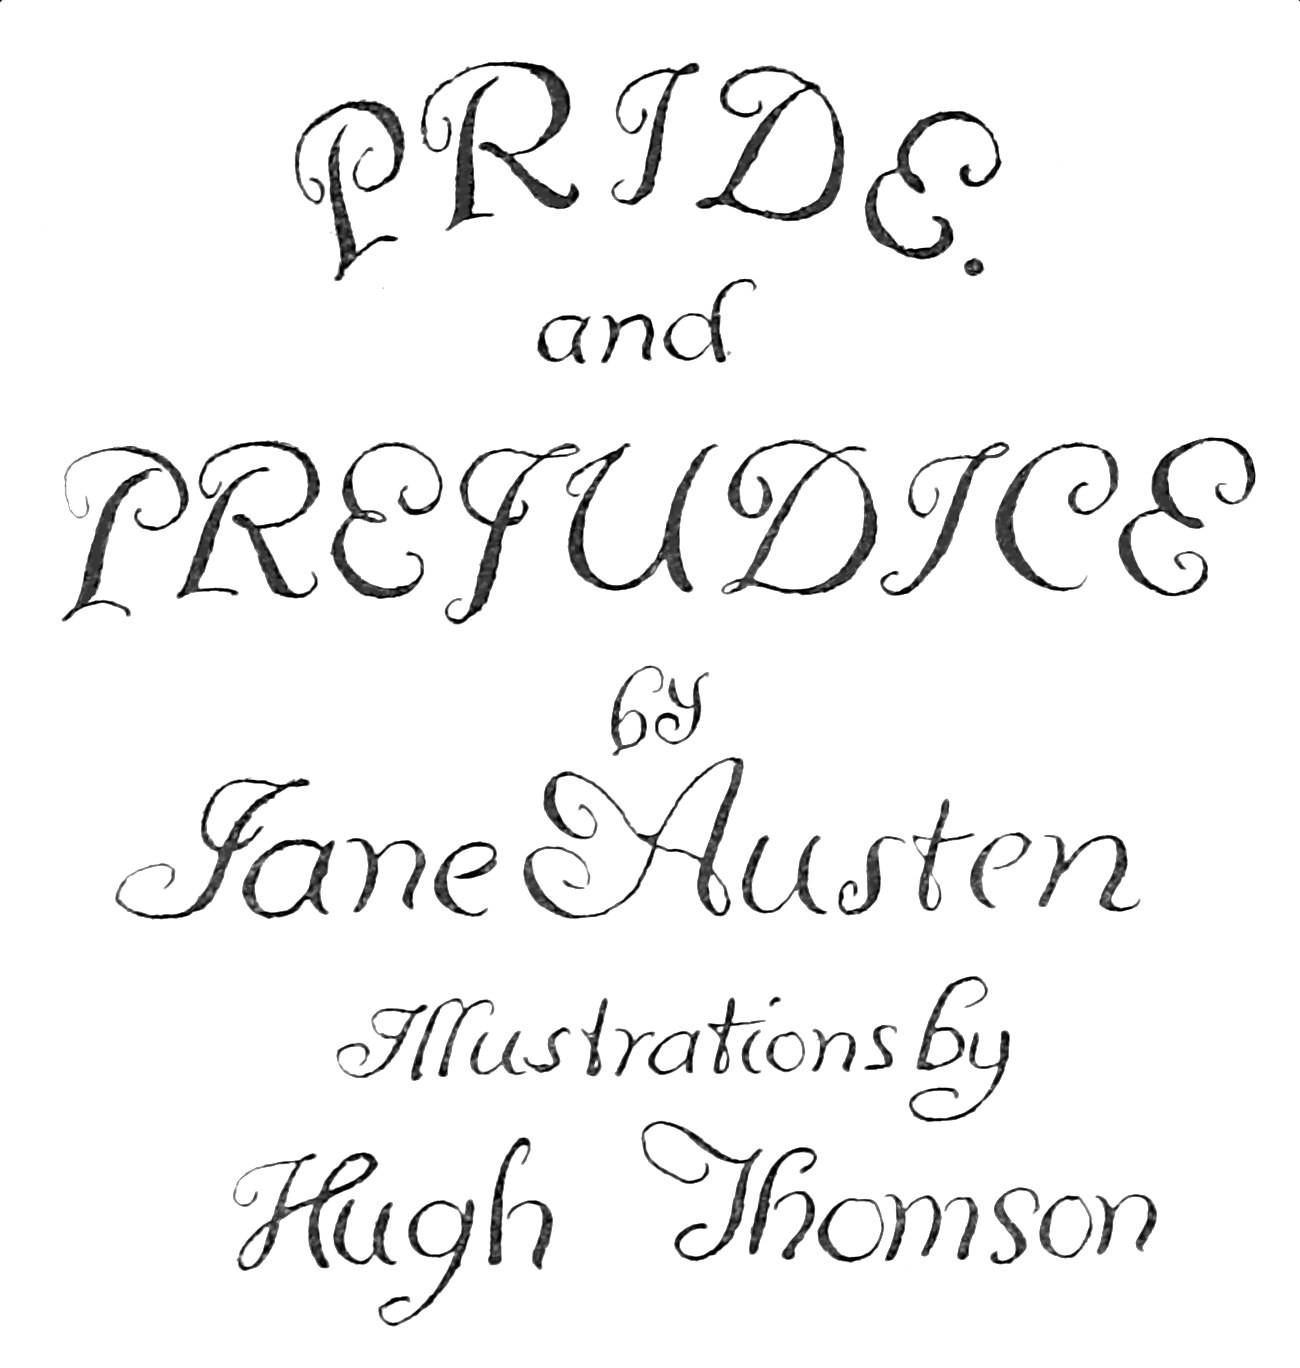
\includepdf[width=.5\textwidth]{halftitle.png}
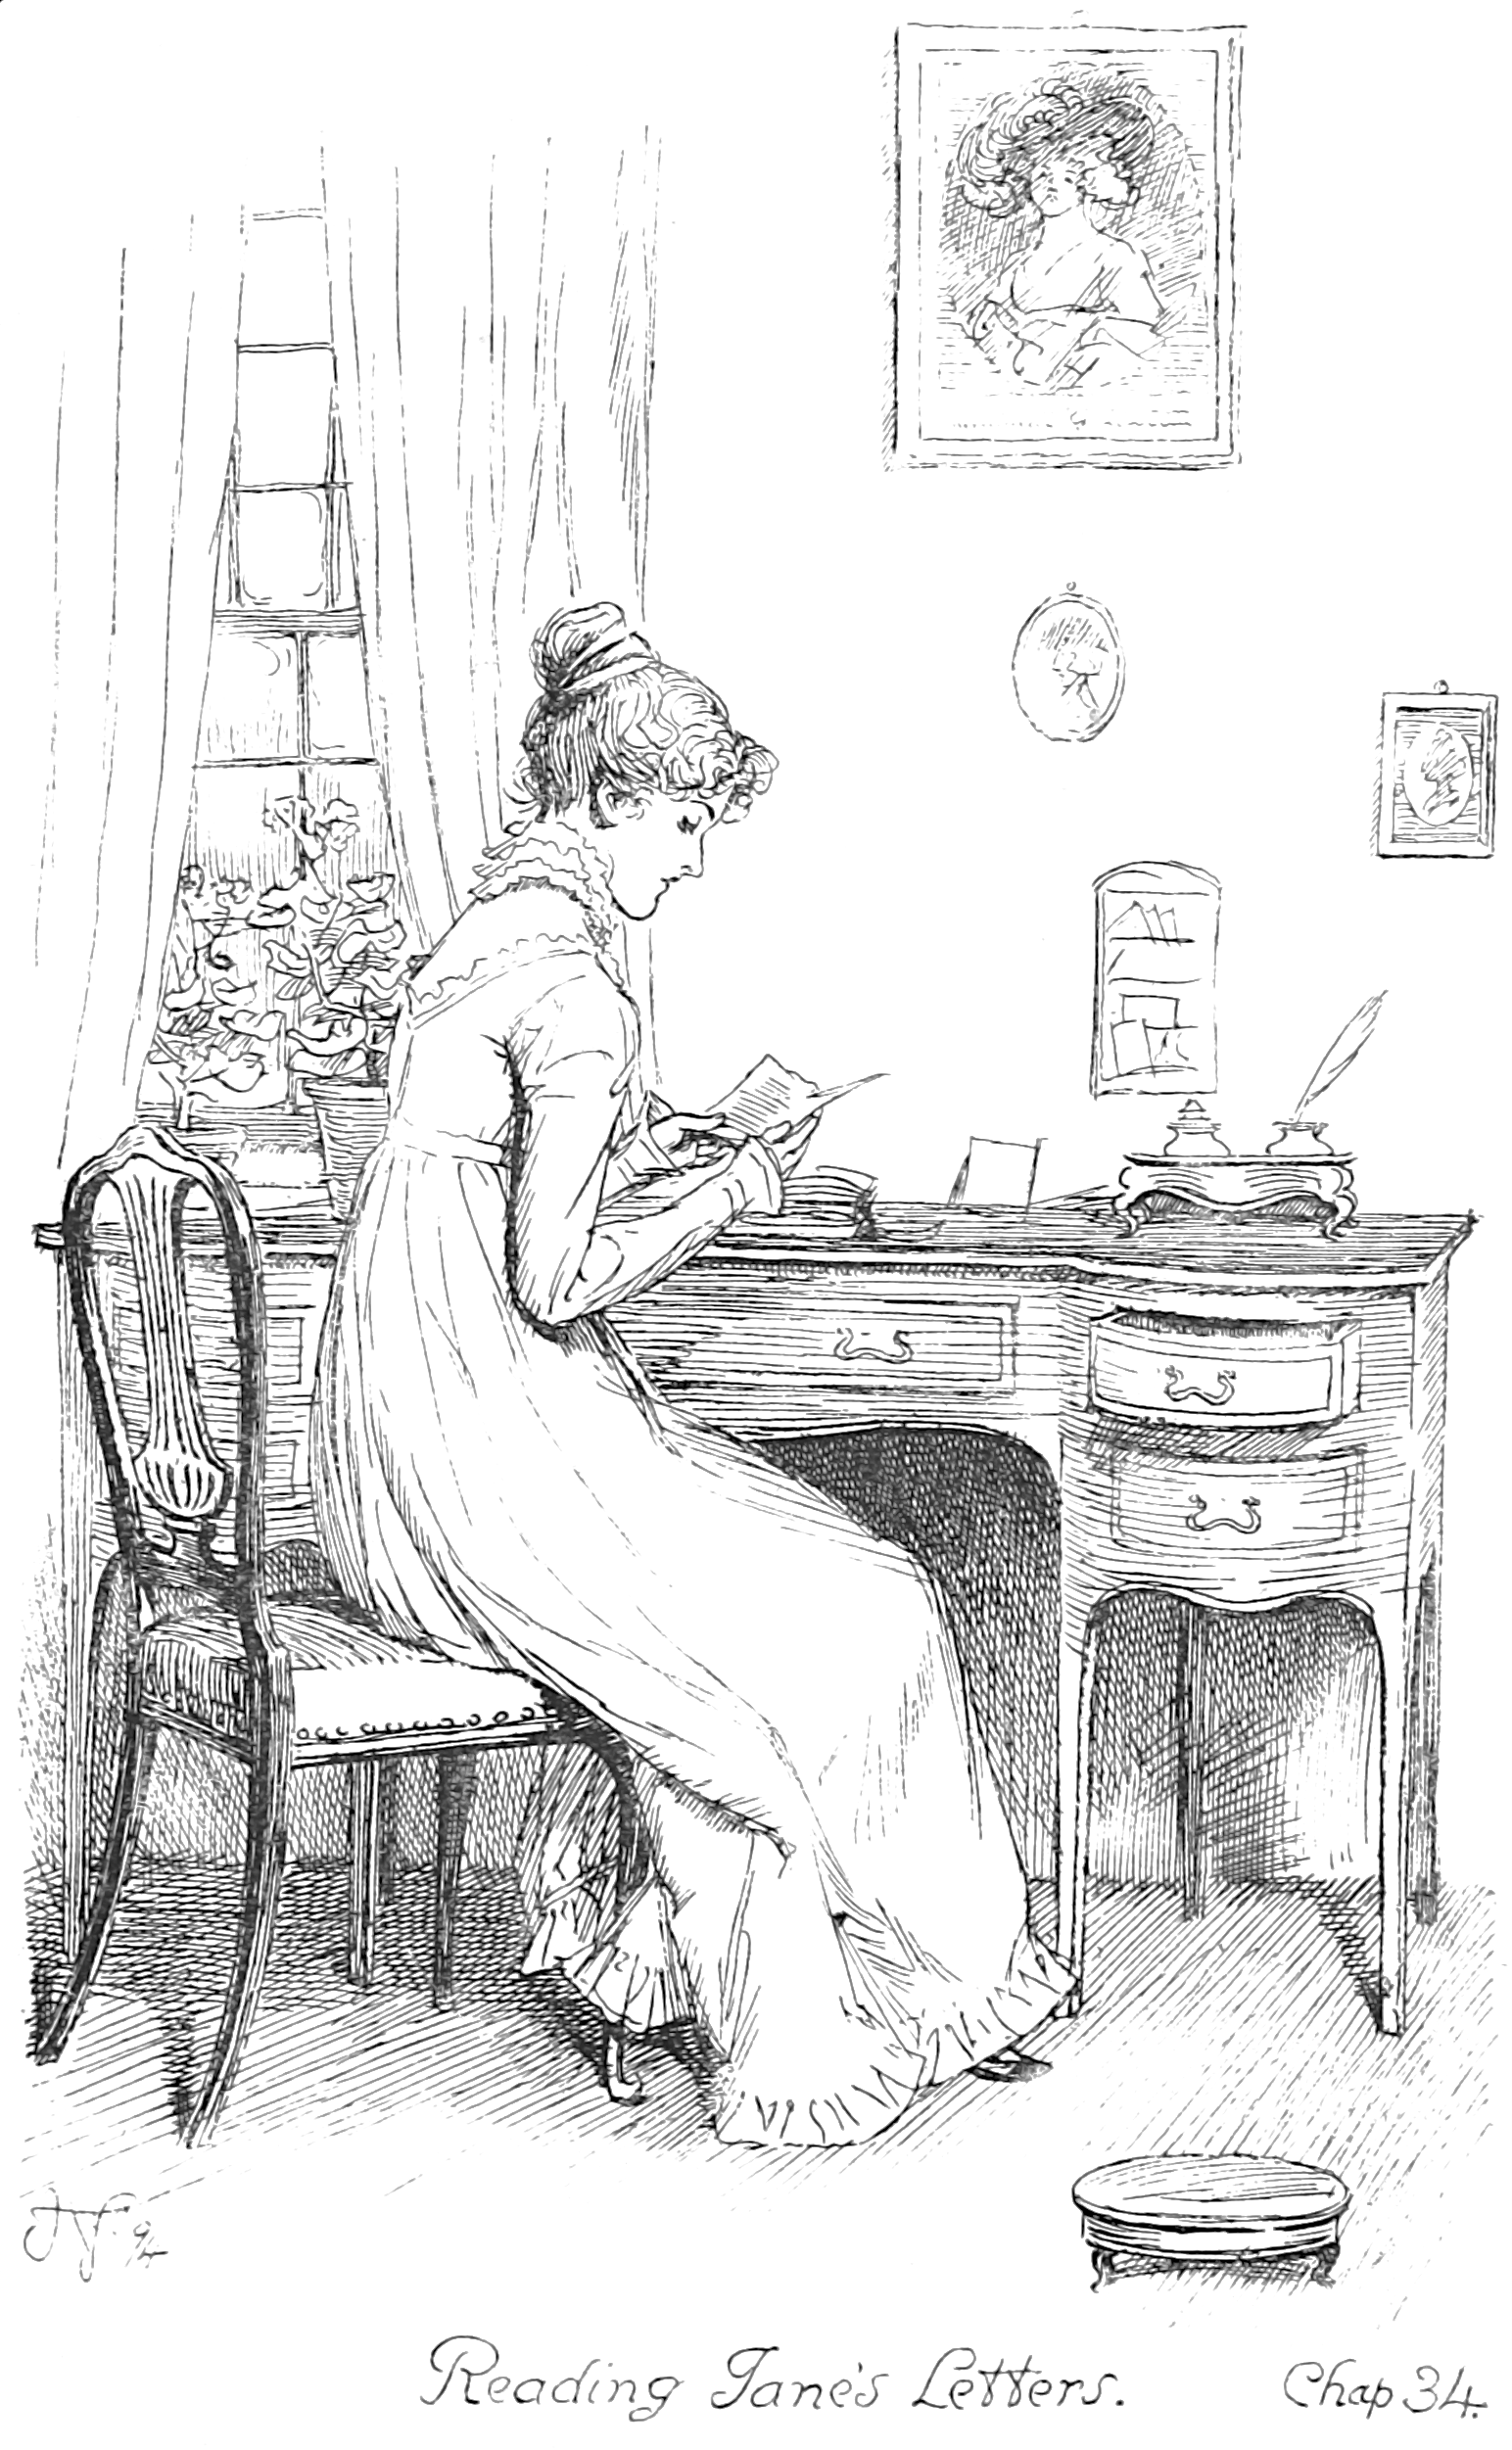
\includepdf[width=\textwidth]{frontispiece.png}
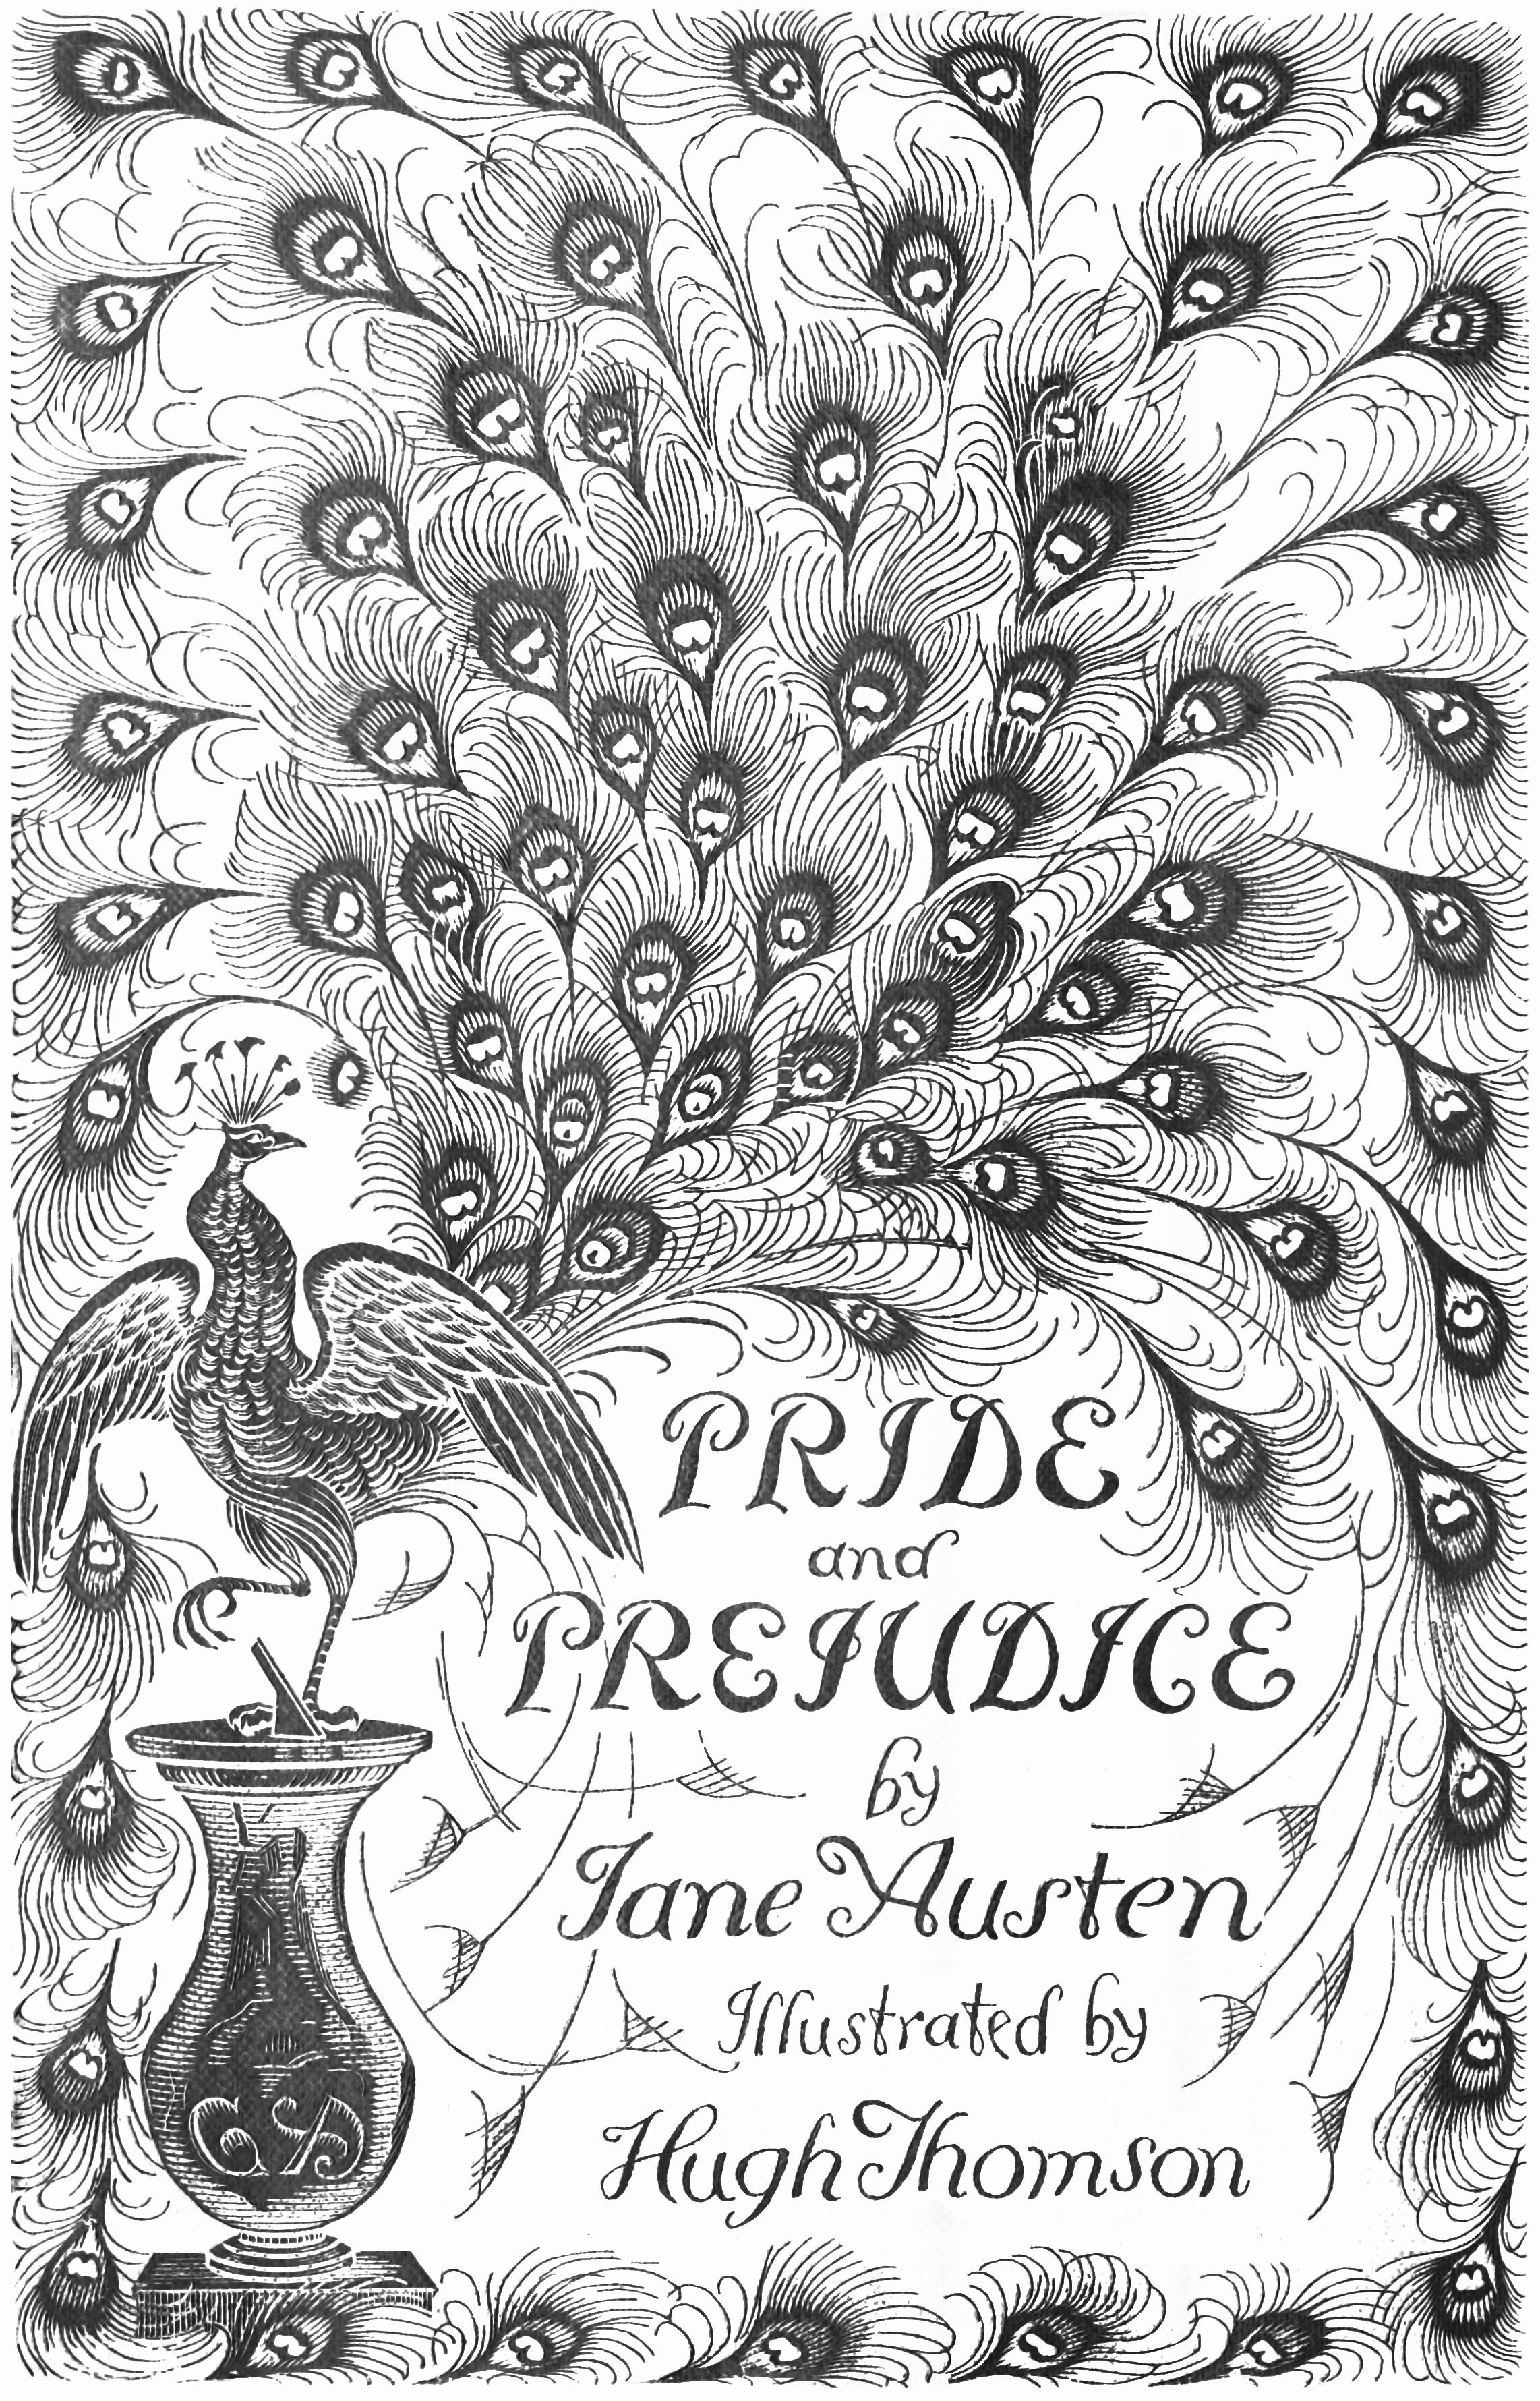
\includepdf[width=1.1\textwidth]{titlepage.jpg}


\renewcommand*\raggedchapter{\centering}
%\KOMAoptions{headings=openright}
%\pagestyle{empty}
%\begin{figure}[p]
%\begin{minipage}[c]{\linewidth}
%\includegraphics[width=\linewidth]{newaccfront}
%\end{minipage}
%\end{figure}
\renewcommand*{\chaptermarkformat}{}
\renewcommand*{\chapterheadendvskip}{\vspace{0pt}}
\renewcommand*{\chapterheadstartvskip}{\vspace{0pt}} %because all chapters have head artwork, no need for whitespace
\KOMAoptions{headings=openleft}

%\renewcommand*{\chapterpagestyle}{empty}
\renewcommand{\contentsname}{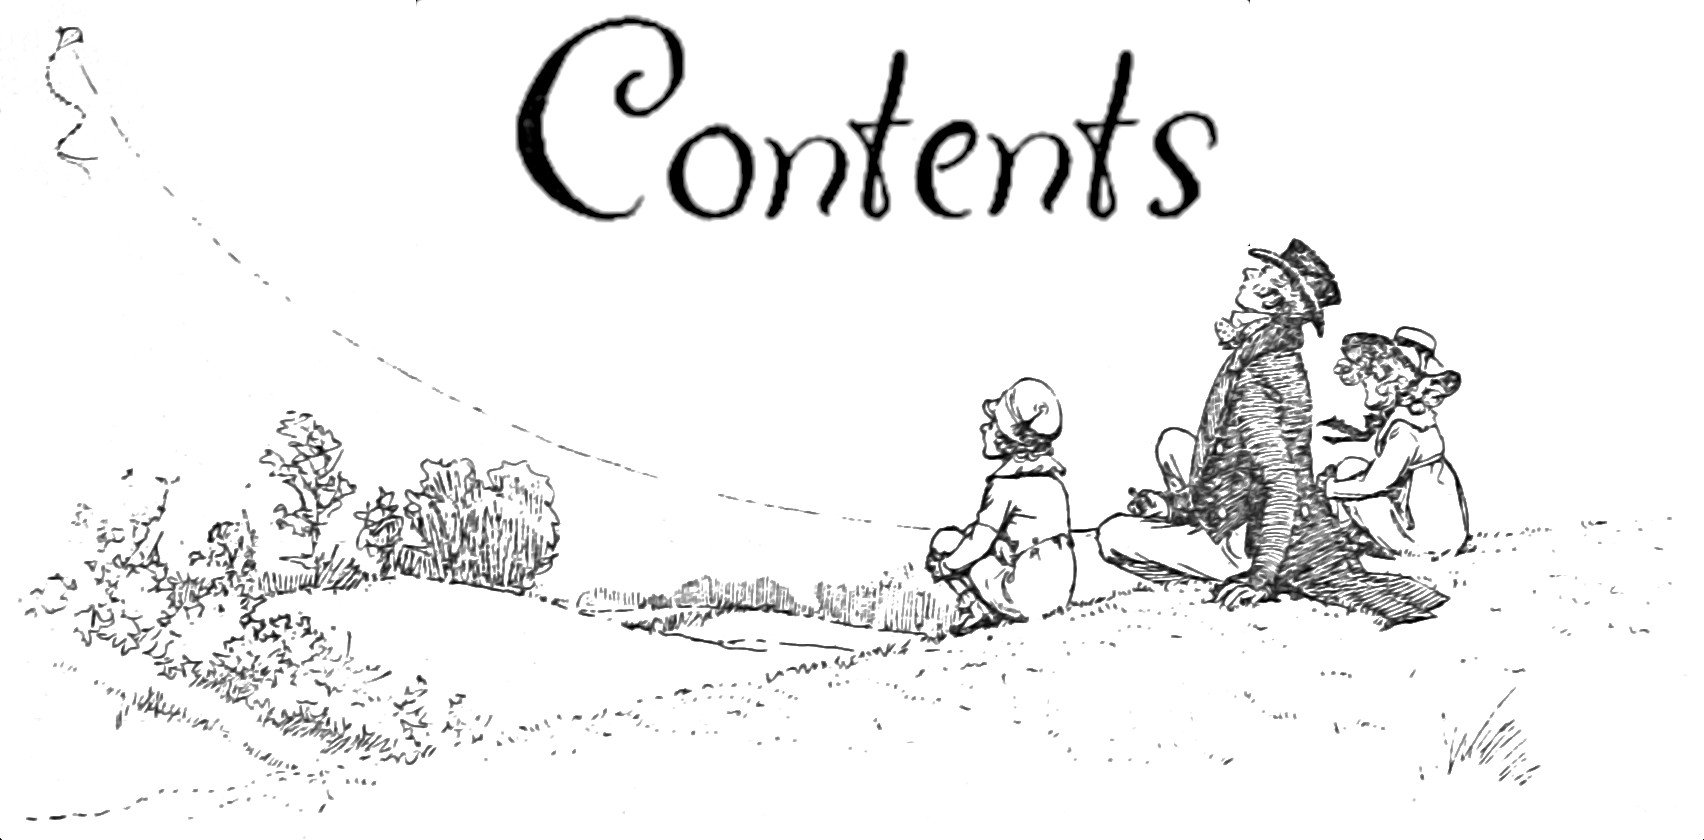
\includegraphics[width=\linewidth]{contents}}
\tableofcontents
\clearpage

%\unsettoc{lof}{chapteratlist}
%\DeclareNewTOC[options ]{extension }
\renewcommand{\listfigurename}{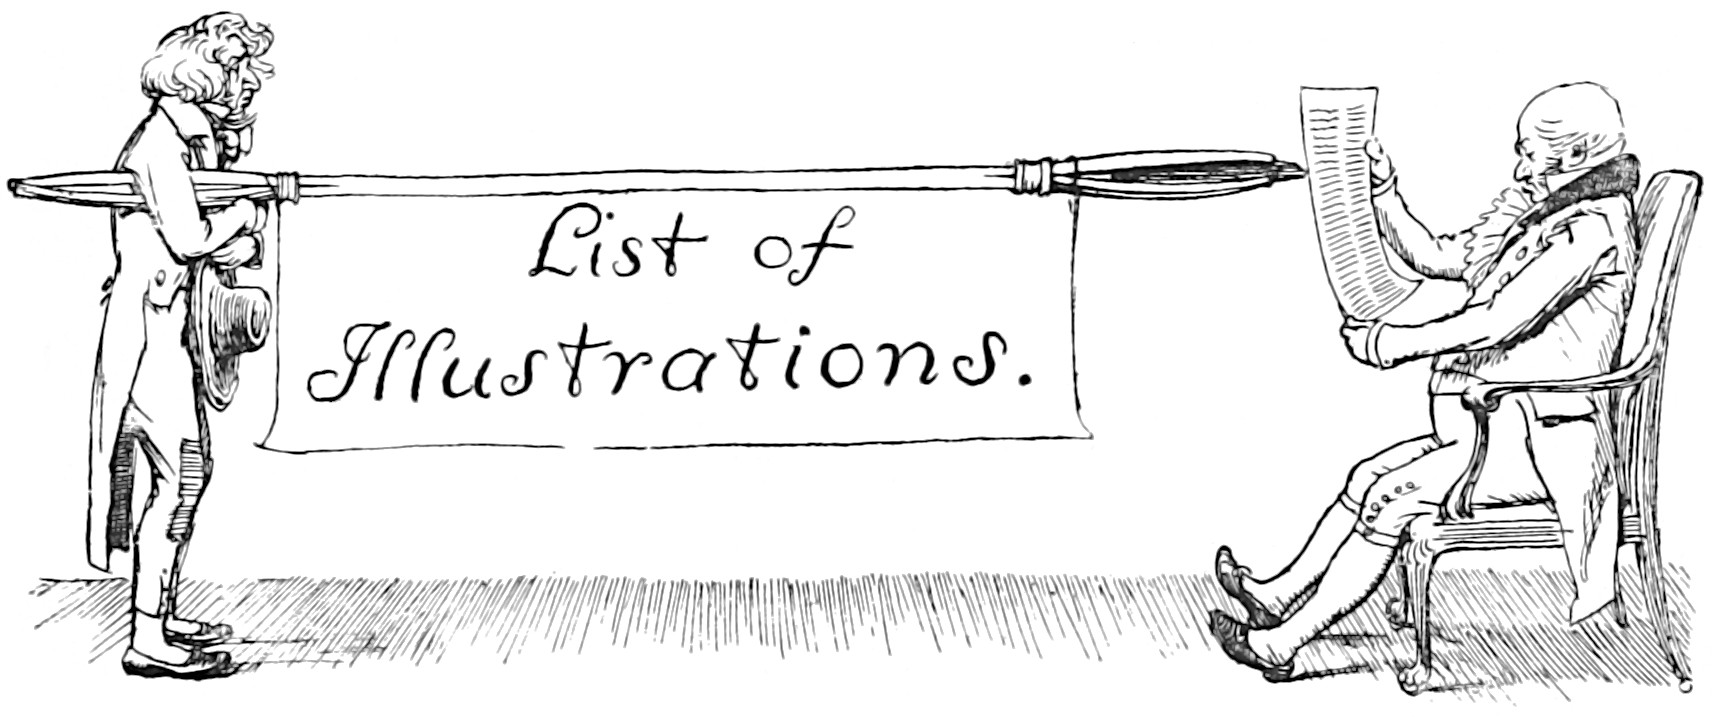
\includegraphics[width=\linewidth]{illustrations}}
\listoffigures
\clearpage

\pagestyle{headings}
\renewcommand*{\chapterpagestyle}{plain}
\newcommand{\moderatelyhuge}{\fontsize{40}{50}\selectfont}



\KOMAoptions{headings=openright}


 
 \mainmatter

%!TeX root=../pridetop.tex

\headlesschapter{Chapter \thechapter}

\begin{pictures}
\begin{a4}
	\begin{figure}[t!]
		\centering
		\captionlistentry{Headpiece to Chapter \thechapter}
		\begin{tikzpicture}[remember picture, overlay]  
			\node (img) at ($(current page.north)+(0cm,-10.5cm)$) {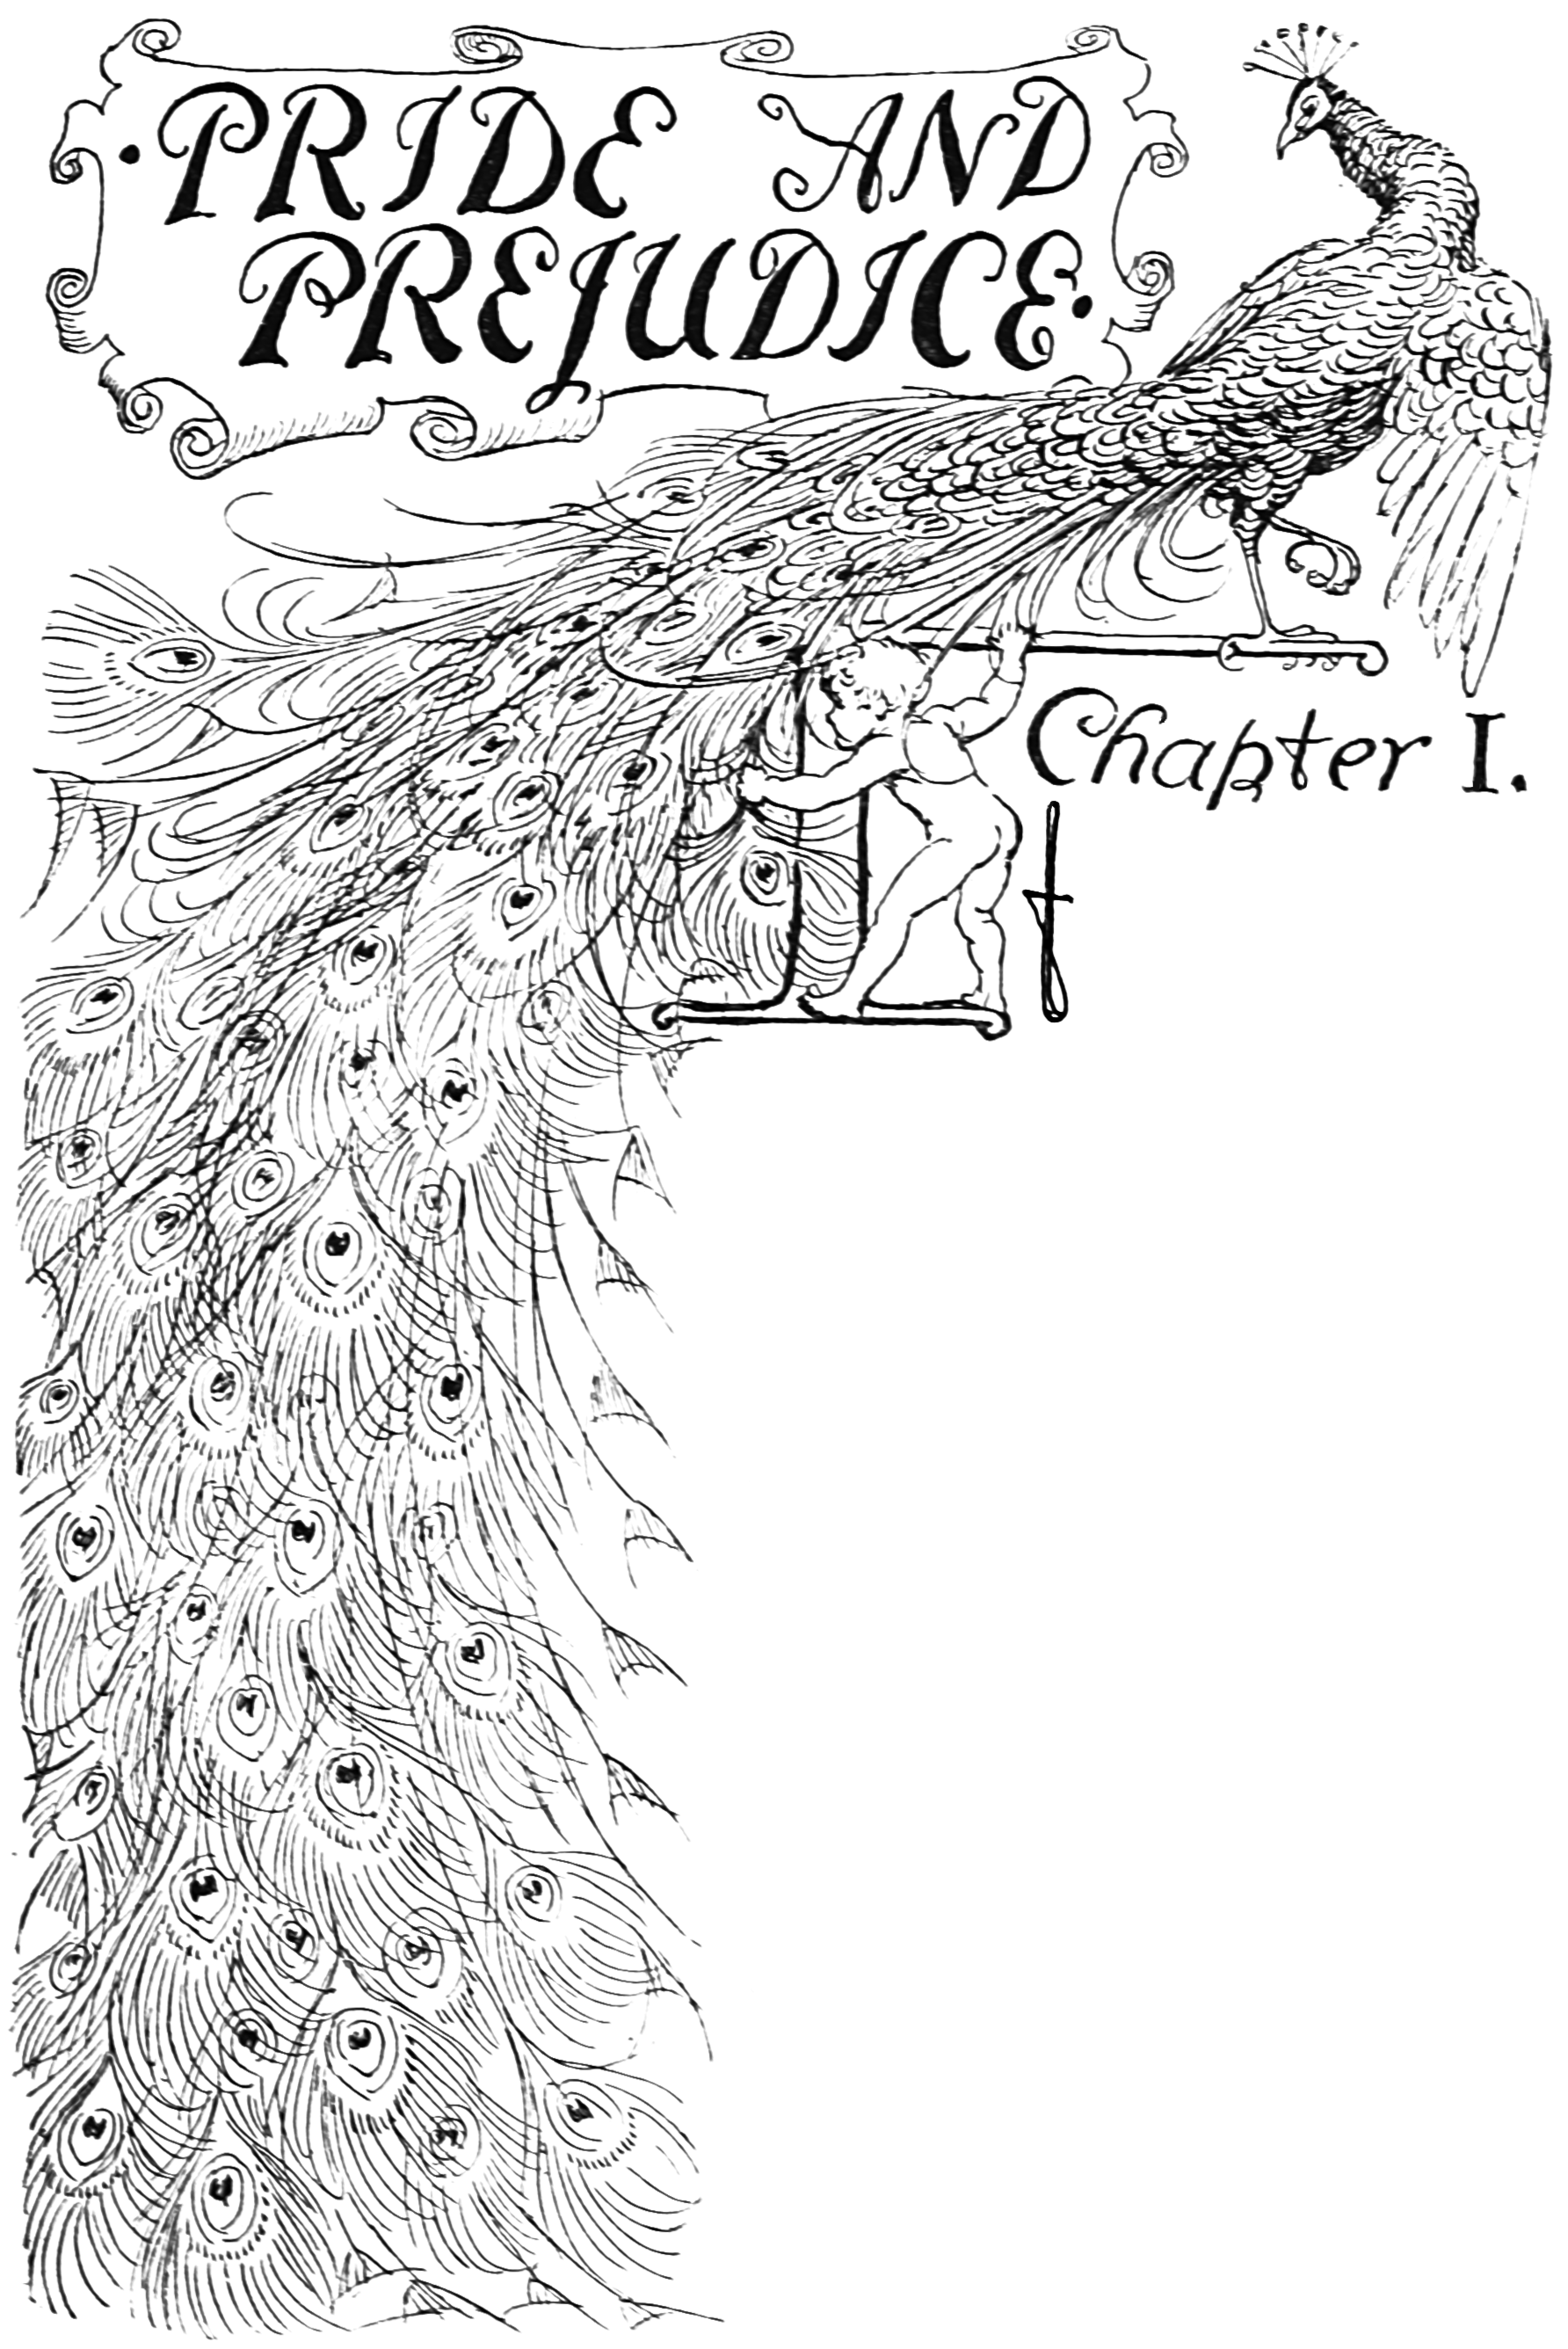
\includegraphics[width=1.15\linewidth]{1top}};
			\node[text width=0.26\textwidth, align=justify] (toptext) at (4.1,1.5) {is a truth universally acknowledged, that};
			\node[below=5.5cm of toptext.east, anchor=east, text width=0.48\textwidth,align=justify] (bottomtext) {
	a single man in possession of a good fortune must be in want of a wife. However little known the feelings or views of such a man may be on his first entering a neighbourhood, this truth is so well fixed in the minds of the surrounding families, that he is considered as the rightful property of some one or other of their daughters.
			\parindent=1em

			<My dear Mr Bennet,> said his lady to him one day, <have you heard that Netherfield Park is let at last?>

			Mr Bennet replied that he had not.

			<But it is,> returned she; <for Mrs Long has just been here, and she told me all about it.>

			Mr Bennet made no answer.

			<Do not you want to know who has taken it?> cried his wife, impatiently.

			<You want to tell me, and I have no objection to hearing it.>
			};
		\end{tikzpicture}
	\end{figure}
\end{a4}

\begin{letter}
	 
	\begin{figure}[t!]
		\centering
		\captionlistentry{Headpiece to Chapter \thechapter}
		\begin{tikzpicture}[remember picture, overlay]
	  
			\node (img) at ($(current page.north)+(0cm,-10.5cm)$) {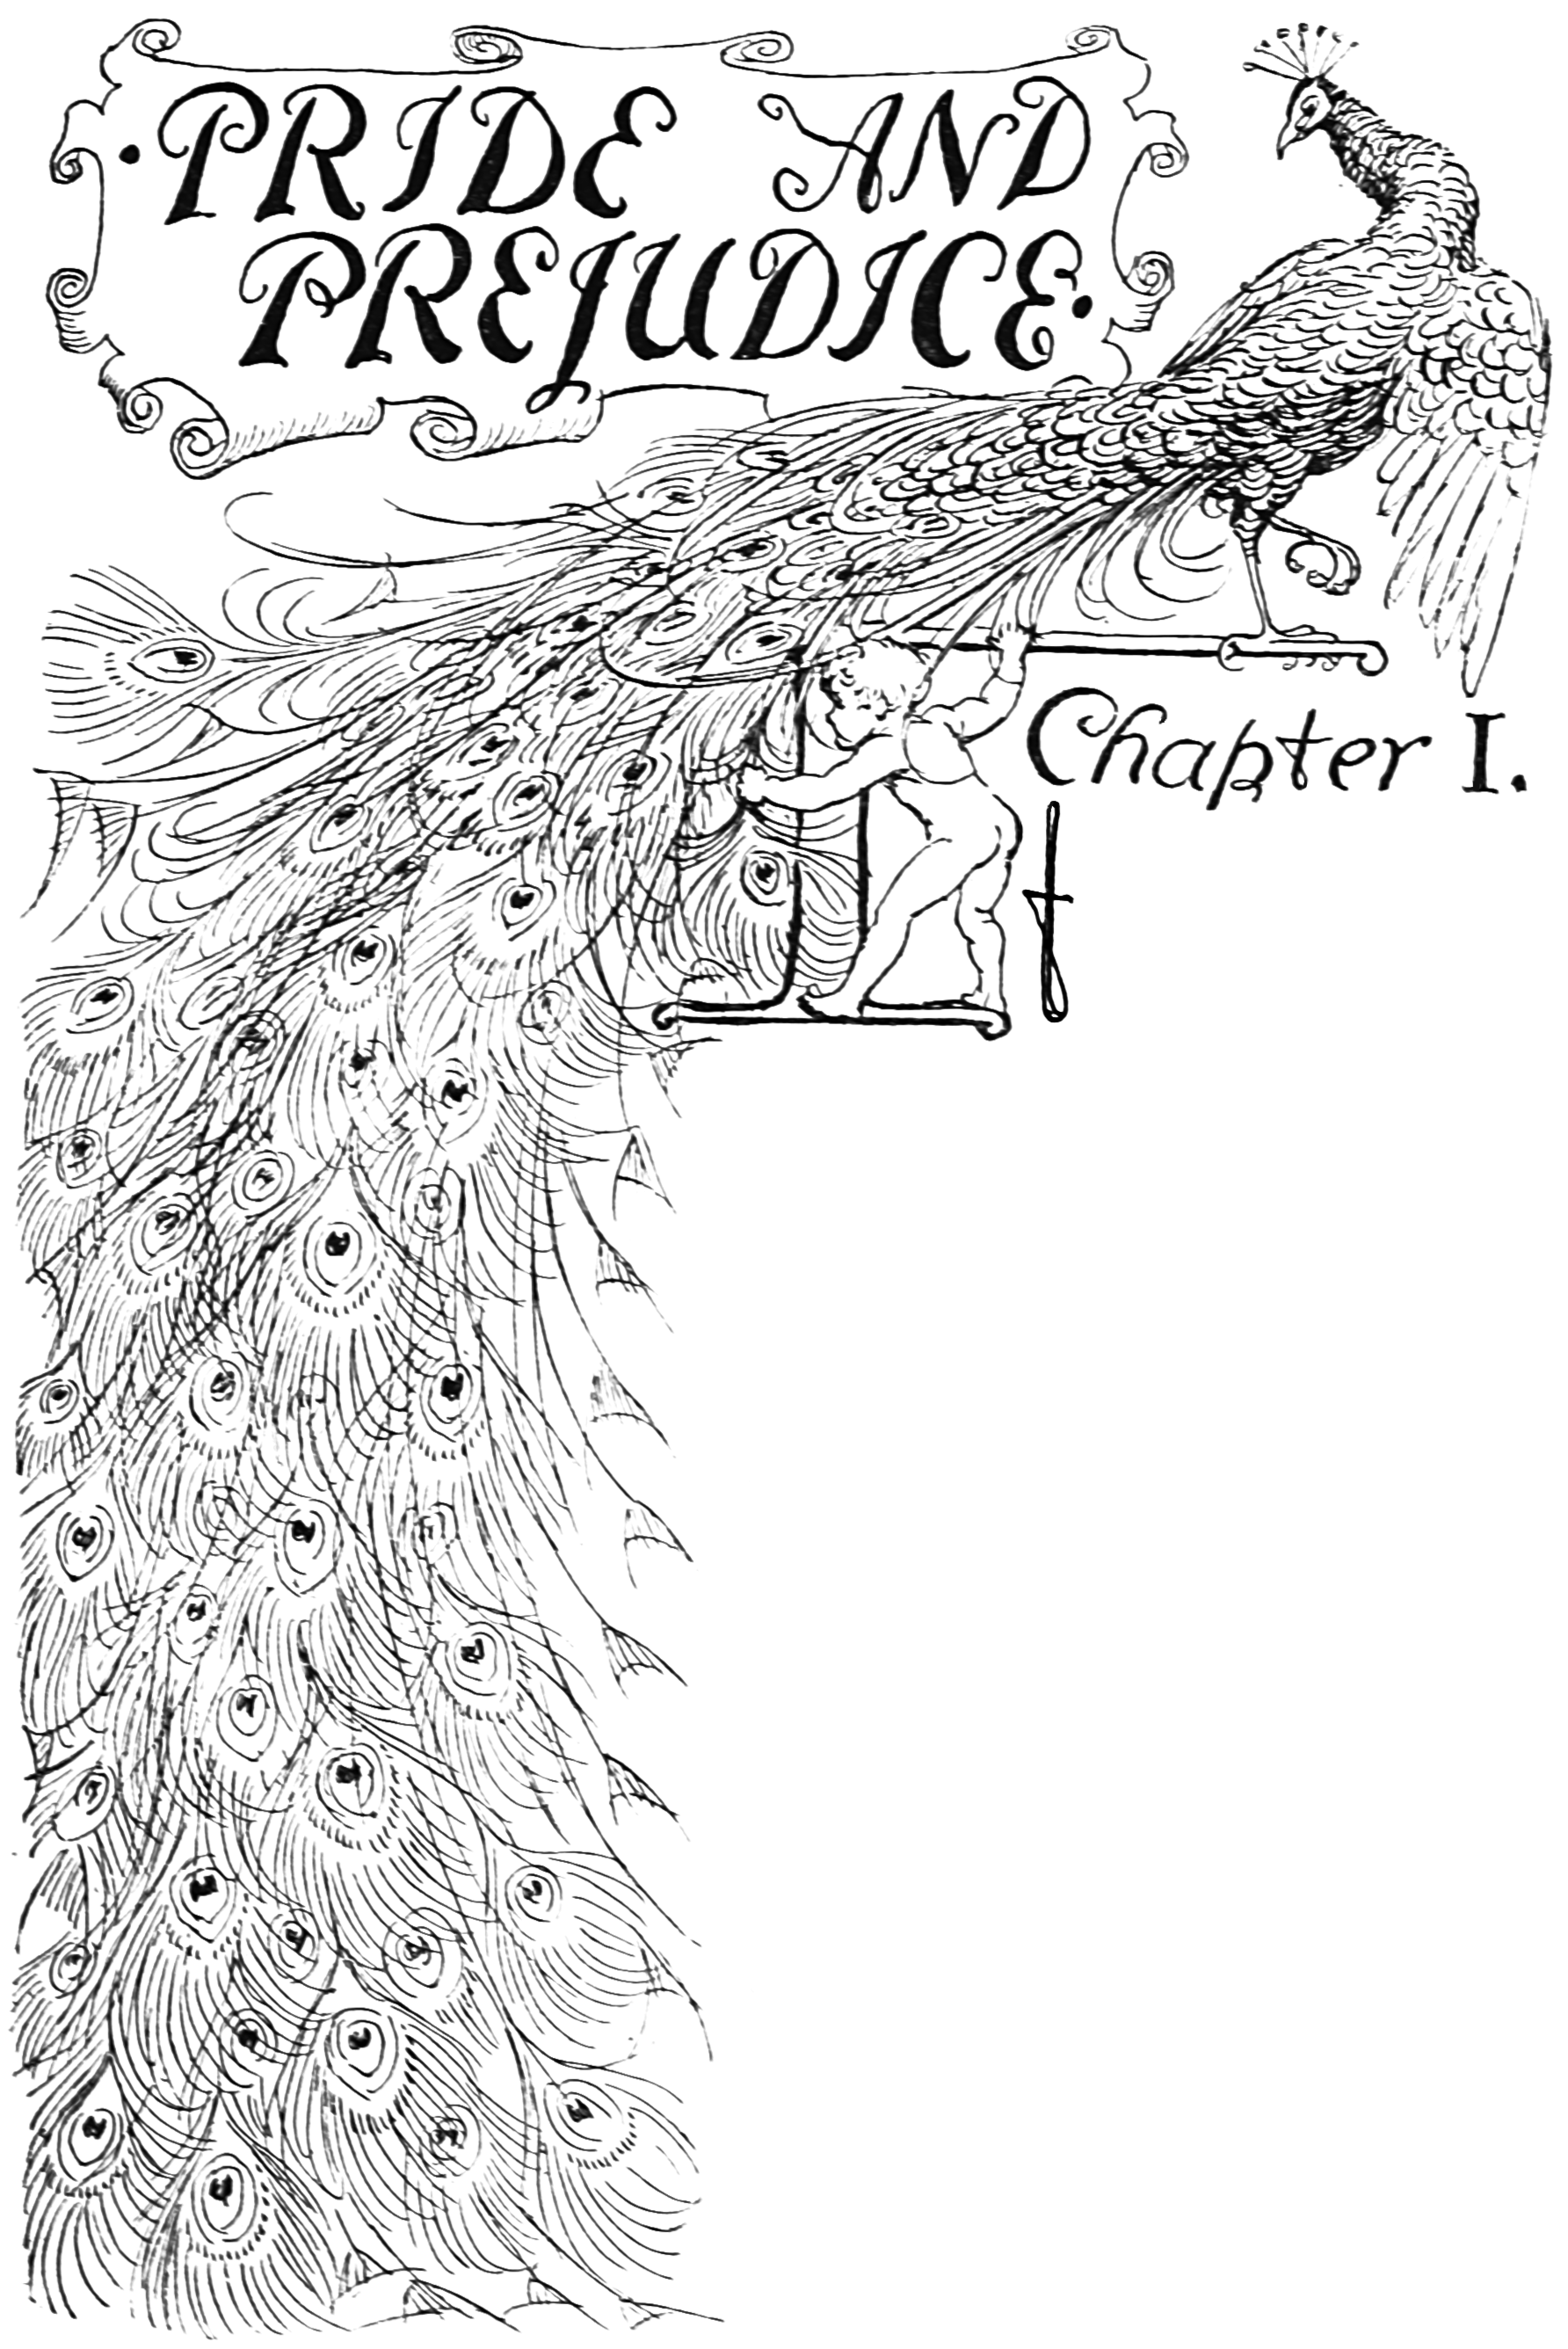
\includegraphics[width=1.2\linewidth]{1top}};
			\node[text width=0.3\textwidth, align=justify] (toptext) at (4.2,1.8) {is a truth universally acknowledged, that a};
			\node[below=5.52cm of toptext.east, anchor=east, text width=0.55\textwidth,align=justify] (bottomtext) {
	single man in possession of a good fortune must be in want of a wife. However little known the feelings or views of such a man may be on his first entering a neighbourhood, this truth is so well fixed in the minds of the surrounding families, that he is considered as the rightful property of some one or other of their daughters.
			\parindent=1em

			<My dear Mr Bennet,> said his lady to him one day, <have you heard that Netherfield Park is let at last?>

			Mr Bennet replied that he had not.

			<But it is,> returned she; <for Mrs Long has just been here, and she told me all about it.>

			Mr Bennet made no answer.

			<Do not you want to know who has taken it?> cried his wife, impatiently.

			<You want to tell me, and I have no objection to hearing it.>
			};
		\end{tikzpicture}
	\end{figure}
%	\enlargethispage{3cm}
\end{letter}

 \thispagestyle{plain}
 \clearpage
\end{pictures}

\begin{placeholder}
It is a truth universally acknowledged, that a single man in possession of a good fortune must be in want of a wife. However little known the feelings or views of such a man may be on his first entering a neighbourhood, this truth is so well fixed in the minds of the surrounding families, that he is considered as the rightful property of some one or other of their daughters.

<My dear Mr Bennet,> said his lady to him one day, <have you heard that Netherfield Park is let at last?>

Mr Bennet replied that he had not.

<But it is,> returned she; <for Mrs Long has just been here, and she told me all about it.>

Mr Bennet made no answer.
<Do not you want to know who has taken it?> cried his wife, impatiently.

<You want to tell me, and I have no objection to hearing it.>
\clearpage
\end{placeholder}

This was invitation enough.

<Why, my dear, you must know, Mrs Long says that Netherfield is taken by a young man of large fortune from the north of England; that he came down on Monday in a chaise and four to see the place, and was so much delighted with it that he agreed with Mr Morris immediately; that he is to take possession before Michaelmas, and some of his servants are to be in the house by the end of next week.>

\begin{figure}[tbh]
\centering
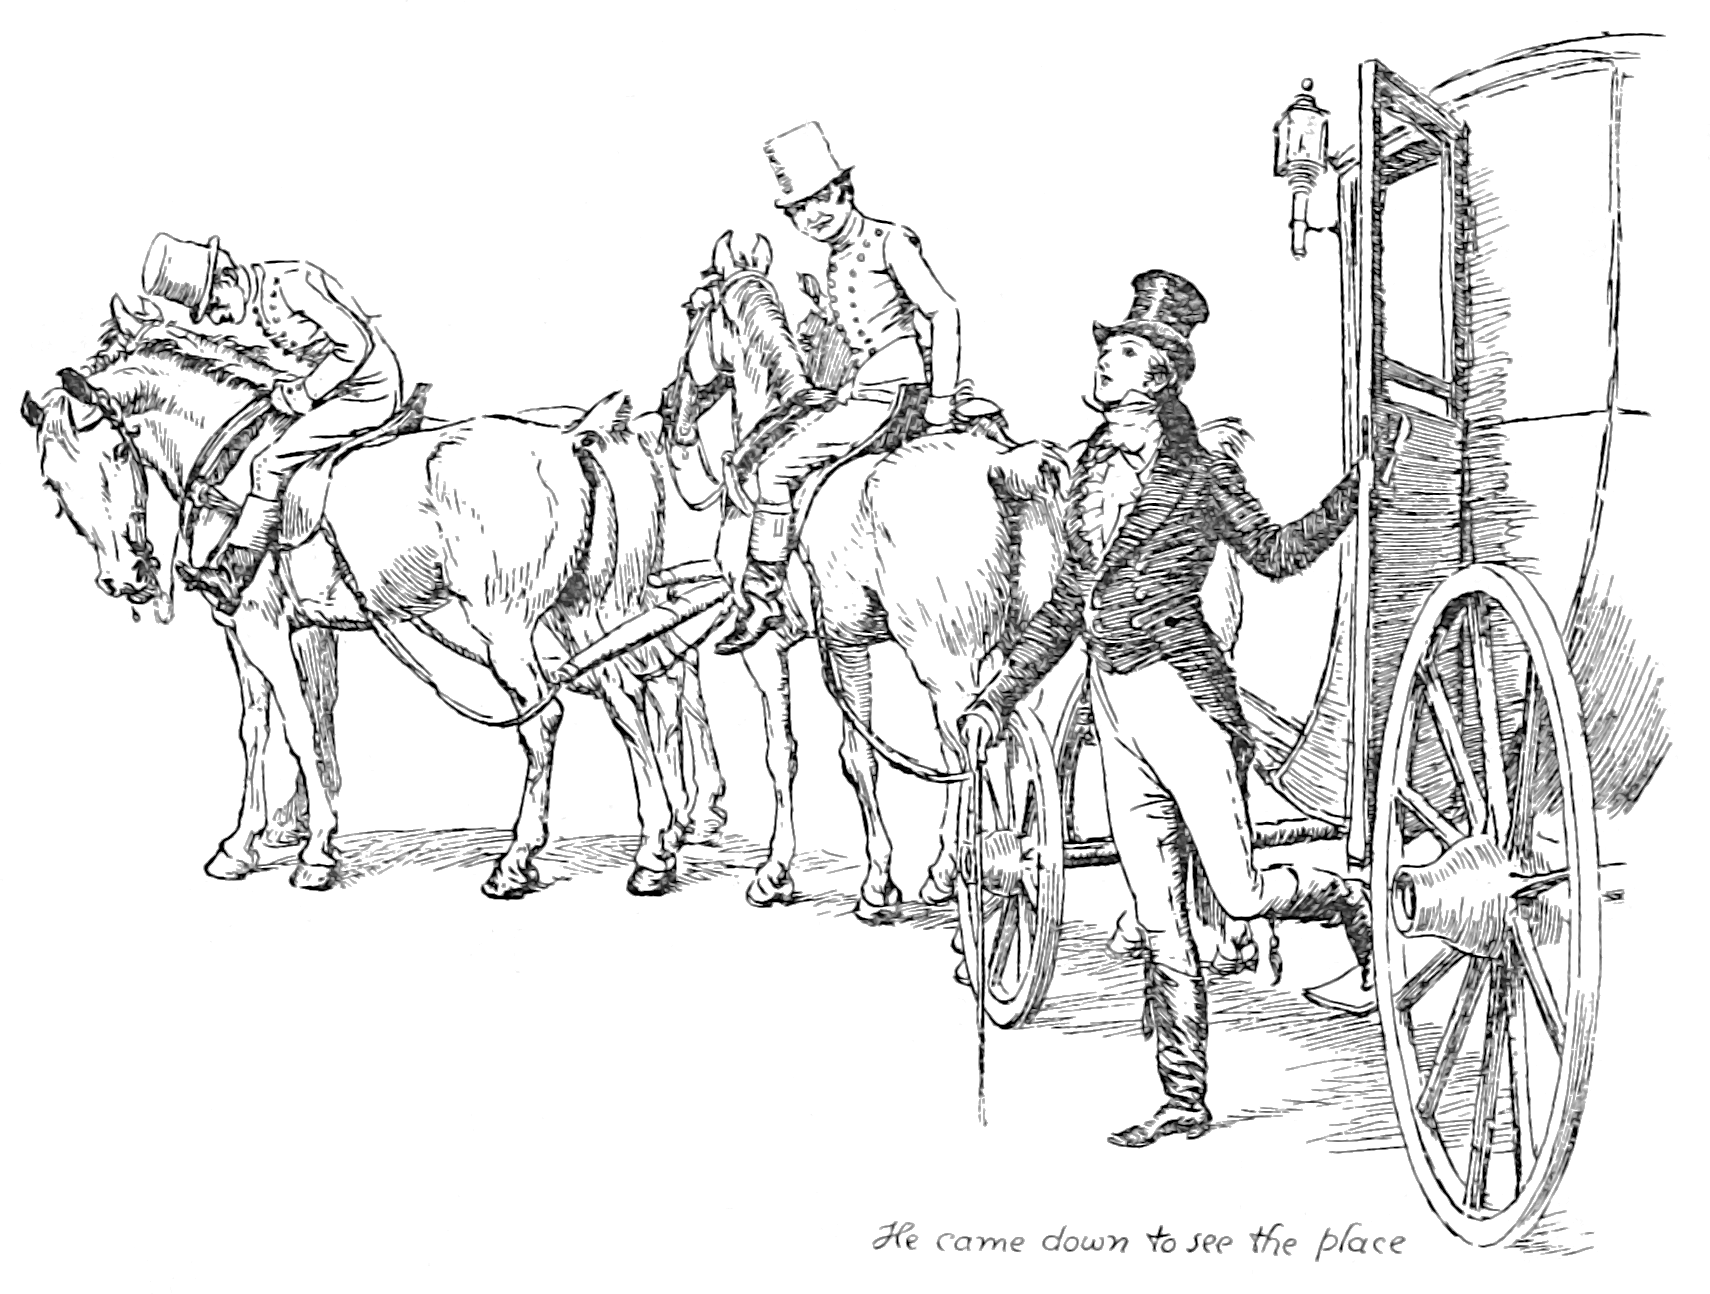
\includegraphics[width=\linewidth]{1camedown}
\captionlistentry{He came down to see the place}
\end{figure}

<What is his name?>

<Bingley.>

<Is he married or single?>

<Oh, single, my dear, to be sure! A single man of large fortune; four or five thousand a year. What a fine thing for our girls!>

<How so? how can it affect them?>

<My dear Mr Bennet,> replied his wife, <how can you be so tiresome? You must know that I am thinking of his marrying one of them.>

<Is that his design in settling here?>

<Design? Nonsense, how can you talk so! But it is very likely that he \textit{may} fall in love with one of them, and therefore you must visit him as soon as he comes.>

<I see no occasion for that. You and the girls may go—or you may send them by themselves, which perhaps will be still better; for as you are as handsome as any of them, Mr Bingley might like you the best of the party.>

<My dear, you flatter me. I certainly \textit{have} had my share of beauty, but I do not pretend to be anything extraordinary now. When a woman has five grown-up daughters, she ought to give over thinking of her own beauty.>

<In such cases, a woman has not often much beauty to think of.>

<But, my dear, you must indeed go and see Mr Bingley when he comes into the neighbourhood.>

<It is more than I engage for, I assure you.>

<But consider your daughters. Only think what an establishment it would be for one of them. Sir William and Lady Lucas are determined to go, merely on that account; for in general, you know, they visit no new comers. Indeed you must go, for it will be impossible for \textit{us} to visit him, if you do not.>

<You are over scrupulous, surely. I dare say Mr Bingley will be very glad to see you; and I will send a few lines by you to assure him of my hearty consent to his marrying whichever he chooses of the girls—though I must throw in a good word for my little Lizzy.>

\begin{figure}[bh!]
\centering
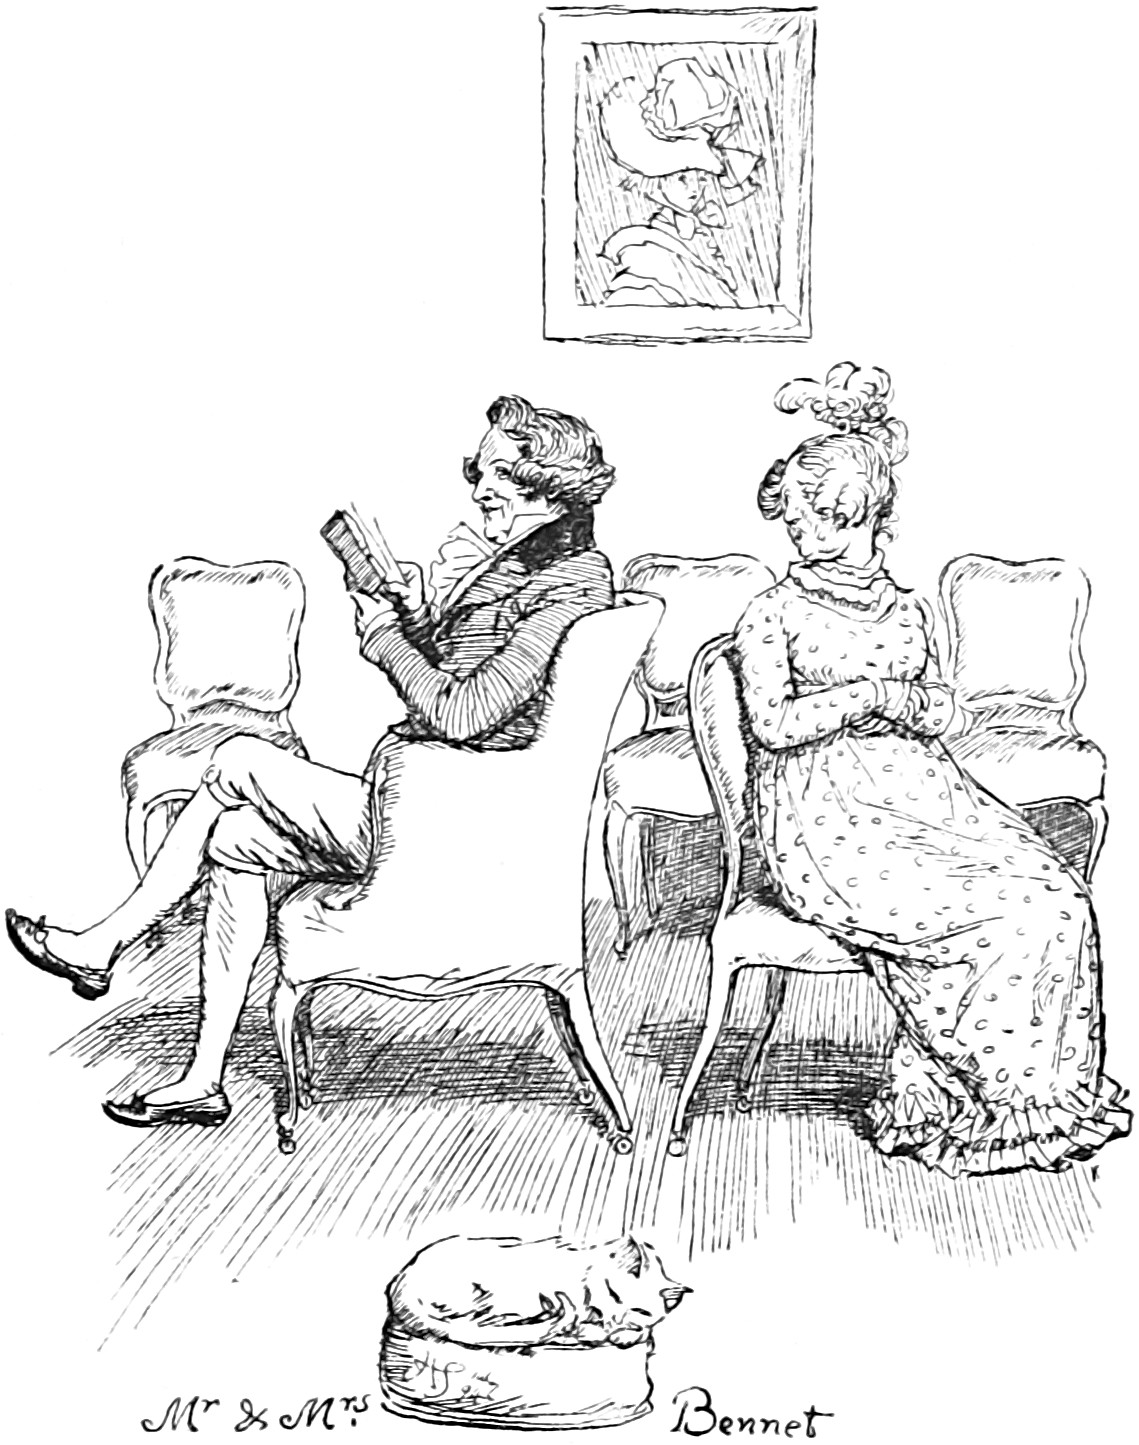
\includegraphics[width=.8\linewidth]{1mrmrs}
\captionlistentry{Mr \& Mrs Bennet}
\end{figure}

<I desire you will do no such thing. Lizzy is not a bit better than the others: and I am sure she is not half so handsome as Jane, nor half so good-humoured as Lydia. But you are always giving \textit{her} the preference.>

<They have none of them much to recommend them,> replied he: <they are all silly and ignorant like other girls; but Lizzy has something more of quickness than her sisters.>

<Mr Bennet, how can you abuse your own children in such a way? You take delight in vexing me. You have no compassion on my poor nerves.>

<You mistake me, my dear. I have a high respect for your nerves. They are my old friends. I have heard you mention them with consideration these twenty years at least.>

<Ah, you do not know what I suffer.>

<But I hope you will get over it, and live to see many young men of four thousand a year come into the neighbourhood.>

<It will be no use to us, if twenty such should come, since you will not visit them.>

<Depend upon it, my dear, that when there are twenty, I will visit them all.>

Mr Bennet was so odd a mixture of quick parts, sarcastic humour, reserve, and caprice, that the experience of three-and-twenty years had been insufficient to make his wife understand his character. \textit{Her} mind was less difficult to develope. She was a woman of mean understanding, little information, and uncertain temper. When she was discontented, she fancied herself nervous. The business of her life was to get her daughters married: its solace was visiting and news.


\chapter[Chapter \thechapter]{} 

 \lettrine[lraise=0.3]{T}{he} little girl performed her long journey in safety; and at Northampton was met by Mrs~Norris, who thus regaled in the credit of being foremost to welcome her, and in the importance of leading her in to the others, and recommending her to their kindness.

Fanny Price was at this time just ten years old, and though there might not be much in her first appearance to captivate, there was, at least, nothing to disgust her relations. She was small of her age, with no glow of complexion, nor any other striking beauty; exceedingly timid and shy, and shrinking from notice; but her air, though awkward, was not vulgar, her voice was sweet, and when she spoke her countenance was pretty. Sir~Thomas and Lady Bertram received her very kindly; and Sir~Thomas, seeing how much she needed encouragement, tried to be all that was conciliating: but he had to work against a most untoward gravity of deportment; and Lady Bertram, without taking half so much trouble, or speaking one word where he spoke ten, by the mere aid of a good-humoured smile, became immediately the less awful character of the two.

The young people were all at home, and sustained their share in the introduction very well, with much good humour, and no embarrassment, at least on the part of the sons, who, at seventeen and sixteen, and tall of their age, had all the grandeur of men in the eyes of their little cousin. The two girls were more at a loss from being younger and in greater awe of their father, who addressed them on the occasion with rather an injudicious particularity. But they were too much used to company and praise to have anything like natural shyness; and their confidence increasing from their cousin's total want of it, they were soon able to take a full survey of her face and her frock in easy indifference.

They were a remarkably fine family, the sons very well-looking, the daughters decidedly handsome, and all of them well-grown and forward of their age, which produced as striking a difference between the cousins in person, as education had given to their address; and no one would have supposed the girls so nearly of an age as they really were. There were in fact but two years between the youngest and Fanny. Julia Bertram was only twelve, and Maria but a year older. The little visitor meanwhile was as unhappy as possible. Afraid of everybody, ashamed of herself, and longing for the home she had left, she knew not how to look up, and could scarcely speak to be heard, or without crying. Mrs~Norris had been talking to her the whole way from Northampton of her wonderful good fortune, and the extraordinary degree of gratitude and good behaviour which it ought to produce, and her consciousness of misery was therefore increased by the idea of its being a wicked thing for her not to be happy. The fatigue, too, of so long a journey, became soon no trifling evil. In vain were the well-meant condescensions of Sir~Thomas, and all the officious prognostications of Mrs~Norris that she would be a good girl; in vain did Lady Bertram smile and make her sit on the sofa with herself and pug, and vain was even the sight of a gooseberry tart towards giving her comfort; she could scarcely swallow two mouthfuls before tears interrupted her, and sleep seeming to be her likeliest friend, she was taken to finish her sorrows in bed.

<This is not a very promising beginning,> said Mrs~Norris, when Fanny had left the room. <After all that I said to her as we came along, I thought she would have behaved better; I told her how much might depend upon her acquitting herself well at first. I wish there may not be a little sulkiness of temper—her poor mother had a good deal; but we must make allowances for such a child—and I do not know that her being sorry to leave her home is really against her, for, with all its faults, it \textit{was}  her home, and she cannot as yet understand how much she has changed for the better; but then there is moderation in all things.>

It required a longer time, however, than Mrs~Norris was inclined to allow, to reconcile Fanny to the novelty of Mansfield Park, and the separation from everybody she had been used to. Her feelings were very acute, and too little understood to be properly attended to. Nobody meant to be unkind, but nobody put themselves out of their way to secure her comfort.

The holiday allowed to the Miss~Bertrams the next day, on purpose to afford leisure for getting acquainted with, and entertaining their young cousin, produced little union. They could not but hold her cheap on finding that she had but two sashes, and had never learned French; and when they perceived her to be little struck with the duet they were so good as to play, they could do no more than make her a generous present of some of their least valued toys, and leave her to herself, while they adjourned to whatever might be the favourite holiday sport of the moment, making artificial flowers or wasting gold paper.

Fanny, whether near or from her cousins, whether in the schoolroom, the drawing-room, or the shrubbery, was equally forlorn, finding something to fear in every person and place. She was disheartened by Lady Bertram's silence, awed by Sir~Thomas's grave looks, and quite overcome by Mrs~Norris's admonitions. Her elder cousins mortified her by reflections on her size, and abashed her by noticing her shyness: Miss~Lee wondered at her ignorance, and the maid-servants sneered at her clothes; and when to these sorrows was added the idea of the brothers and sisters among whom she had always been important as playfellow, instructress, and nurse, the despondence that sunk her little heart was severe.

The grandeur of the house astonished, but could not console her. The rooms were too large for her to move in with ease: whatever she touched she expected to injure, and she crept about in constant terror of something or other; often retreating towards her own chamber to cry; and the little girl who was spoken of in the drawing-room when she left it at night as seeming so desirably sensible of her peculiar good fortune, ended every day's sorrows by sobbing herself to sleep. A week had passed in this way, and no suspicion of it conveyed by her quiet passive manner, when she was found one morning by her cousin Edmund, the youngest of the sons, sitting crying on the attic stairs.

<My dear little cousin,> said he, with all the gentleness of an excellent nature, <what can be the matter?> And sitting down by her, he was at great pains to overcome her shame in being so surprised, and persuade her to speak openly. Was she ill? or was anybody angry with her? or had she quarrelled with Maria and Julia? or was she puzzled about anything in her lesson that he could explain? Did she, in short, want anything he could possibly get her, or do for her? For a long while no answer could be obtained beyond a <no, no—not at all—no, thank you>; but he still persevered; and no sooner had he begun to revert to her own home, than her increased sobs explained to him where the grievance lay. He tried to console her.

<You are sorry to leave Mama, my dear little Fanny,> said he, <which shows you to be a very good girl; but you must remember that you are with relations and friends, who all love you, and wish to make you happy. Let us walk out in the park, and you shall tell me all about your brothers and sisters.>

On pursuing the subject, he found that, dear as all these brothers and sisters generally were, there was one among them who ran more in her thoughts than the rest. It was William whom she talked of most, and wanted most to see. William, the eldest, a year older than herself, her constant companion and friend; her advocate with her mother (of whom he was the darling) in every distress. <William did not like she should come away; he had told her he should miss her very much indeed.> <But William will write to you, I dare say.> <Yes, he had promised he would, but he had told \textit{her}  to write first.> <And when shall you do it?> She hung her head and answered hesitatingly, <she did not know; she had not any paper.>

<If that be all your difficulty, I will furnish you with paper and every other material, and you may write your letter whenever you choose. Would it make you happy to write to William?>

<Yes, very.>

<Then let it be done now. Come with me into the breakfast-room, we shall find everything there, and be sure of having the room to ourselves.>

<But, cousin, will it go to the post?>

<Yes, depend upon me it shall: it shall go with the other letters; and, as your uncle will frank it, it will cost William nothing.>

<My uncle!> repeated Fanny, with a frightened look.

<Yes, when you have written the letter, I will take it to my father to frank.>

Fanny thought it a bold measure, but offered no further resistance; and they went together into the breakfast-room, where Edmund prepared her paper, and ruled her lines with all the goodwill that her brother could himself have felt, and probably with somewhat more exactness. He continued with her the whole time of her writing, to assist her with his penknife or his orthography, as either were wanted; and added to these attentions, which she felt very much, a kindness to her brother which delighted her beyond all the rest. He wrote with his own hand his love to his cousin William, and sent him half a guinea under the seal. Fanny's feelings on the occasion were such as she believed herself incapable of expressing; but her countenance and a few artless words fully conveyed all their gratitude and delight, and her cousin began to find her an interesting object. He talked to her more, and, from all that she said, was convinced of her having an affectionate heart, and a strong desire of doing right; and he could perceive her to be farther entitled to attention by great sensibility of her situation, and great timidity. He had never knowingly given her pain, but he now felt that she required more positive kindness; and with that view endeavoured, in the first place, to lessen her fears of them all, and gave her especially a great deal of good advice as to playing with Maria and Julia, and being as merry as possible.

From this day Fanny grew more comfortable. She felt that she had a friend, and the kindness of her cousin Edmund gave her better spirits with everybody else. The place became less strange, and the people less formidable; and if there were some amongst them whom she could not cease to fear, she began at least to know their ways, and to catch the best manner of conforming to them. The little rusticities and awkwardnesses which had at first made grievous inroads on the tranquillity of all, and not least of herself, necessarily wore away, and she was no longer materially afraid to appear before her uncle, nor did her aunt Norris's voice make her start very much. To her cousins she became occasionally an acceptable companion. Though unworthy, from inferiority of age and strength, to be their constant associate, their pleasures and schemes were sometimes of a nature to make a third very useful, especially when that third was of an obliging, yielding temper; and they could not but own, when their aunt inquired into her faults, or their brother Edmund urged her claims to their kindness, that <Fanny was good-natured enough.>

Edmund was uniformly kind himself; and she had nothing worse to endure on the part of Tom than that sort of merriment which a young man of seventeen will always think fair with a child of ten. He was just entering into life, full of spirits, and with all the liberal dispositions of an eldest son, who feels born only for expense and enjoyment. His kindness to his little cousin was consistent with his situation and rights: he made her some very pretty presents, and laughed at her.

As her appearance and spirits improved, Sir~Thomas and Mrs~Norris thought with greater satisfaction of their benevolent plan; and it was pretty soon decided between them that, though far from clever, she showed a tractable disposition, and seemed likely to give them little trouble. A mean opinion of her abilities was not confined to \textit{them}. Fanny could read, work, and write, but she had been taught nothing more; and as her cousins found her ignorant of many things with which they had been long familiar, they thought her prodigiously stupid, and for the first two or three weeks were continually bringing some fresh report of it into the drawing-room. <Dear mama, only think, my cousin cannot put the map of Europe together—or my cousin cannot tell the principal rivers in Russia—or, she never heard of Asia Minor—or she does not know the difference between water-colours and crayons!—How strange!—Did you ever hear anything so stupid?>

<My dear,> their considerate aunt would reply, <it is very bad, but you must not expect everybody to be as forward and quick at learning as yourself.>

<But, aunt, she is really so very ignorant!—Do you know, we asked her last night which way she would go to get to Ireland; and she said, she should cross to the Isle of Wight. She thinks of nothing but the Isle of Wight, and she calls it \textit{the Island}, as if there were no other island in the world. I am sure I should have been ashamed of myself, if I had not known better long before I was so old as she is. I cannot remember the time when I did not know a great deal that she has not the least notion of yet. How long ago it is, aunt, since we used to repeat the chronological order of the kings of England, with the dates of their accession, and most of the principal events of their reigns!>

<Yes,> added the other; <and of the Roman emperors as low as Severus; besides a great deal of the heathen mythology, and all the metals, semi-metals, planets, and distinguished philosophers.>

<Very true indeed, my dears, but you are blessed with wonderful memories, and your poor cousin has probably none at all. There is a vast deal of difference in memories, as well as in everything else, and therefore you must make allowance for your cousin, and pity her deficiency. And remember that, if you are ever so forward and clever yourselves, you should always be modest; for, much as you know already, there is a great deal more for you to learn.>

<Yes, I know there is, till I am seventeen. But I must tell you another thing of Fanny, so odd and so stupid. Do you know, she says she does not want to learn either music or drawing.>

<To be sure, my dear, that is very stupid indeed, and shows a great want of genius and emulation. But, all things considered, I do not know whether it is not as well that it should be so, for, though you know (owing to me) your papa and mama are so good as to bring her up with you, it is not at all necessary that she should be as accomplished as you are;—on the contrary, it is much more desirable that there should be a difference.>

Such were the counsels by which Mrs~Norris assisted to form her nieces' minds; and it is not very wonderful that, with all their promising talents and early information, they should be entirely deficient in the less common acquirements of self-knowledge, generosity and humility. In everything but disposition they were admirably taught. Sir~Thomas did not know what was wanting, because, though a truly anxious father, he was not outwardly affectionate, and the reserve of his manner repressed all the flow of their spirits before him.

To the education of her daughters Lady Bertram paid not the smallest attention. She had not time for such cares. She was a woman who spent her days in sitting, nicely dressed, on a sofa, doing some long piece of needlework, of little use and no beauty, thinking more of her pug than her children, but very indulgent to the latter when it did not put herself to inconvenience, guided in everything important by Sir~Thomas, and in smaller concerns by her sister. Had she possessed greater leisure for the service of her girls, she would probably have supposed it unnecessary, for they were under the care of a governess, with proper masters, and could want nothing more. As for Fanny's being stupid at learning, <she could only say it was very unlucky, but some people \textit{were}  stupid, and Fanny must take more pains: she did not know what else was to be done; and, except her being so dull, she must add she saw no harm in the poor little thing, and always found her very handy and quick in carrying messages, and fetching what she wanted.>

Fanny, with all her faults of ignorance and timidity, was fixed at Mansfield Park, and learning to transfer in its favour much of her attachment to her former home, grew up there not unhappily among her cousins. There was no positive ill-nature in Maria or Julia; and though Fanny was often mortified by their treatment of her, she thought too lowly of her own claims to feel injured by it.

From about the time of her entering the family, Lady Bertram, in consequence of a little ill-health, and a great deal of indolence, gave up the house in town, which she had been used to occupy every spring, and remained wholly in the country, leaving Sir~Thomas to attend his duty in Parliament, with whatever increase or diminution of comfort might arise from her absence. In the country, therefore, the Miss~Bertrams continued to exercise their memories, practise their duets, and grow tall and womanly: and their father saw them becoming in person, manner, and accomplishments, everything that could satisfy his anxiety. His eldest son was careless and extravagant, and had already given him much uneasiness; but his other children promised him nothing but good. His daughters, he felt, while they retained the name of Bertram, must be giving it new grace, and in quitting it, he trusted, would extend its respectable alliances; and the character of Edmund, his strong good sense and uprightness of mind, bid most fairly for utility, honour, and happiness to himself and all his connexions. He was to be a clergyman.

Amid the cares and the complacency which his own children suggested, Sir~Thomas did not forget to do what he could for the children of Mrs~Price: he assisted her liberally in the education and disposal of her sons as they became old enough for a determinate pursuit; and Fanny, though almost totally separated from her family, was sensible of the truest satisfaction in hearing of any kindness towards them, or of anything at all promising in their situation or conduct. Once, and once only, in the course of many years, had she the happiness of being with William. Of the rest she saw nothing: nobody seemed to think of her ever going amongst them again, even for a visit, nobody at home seemed to want her; but William determining, soon after her removal, to be a sailor, was invited to spend a week with his sister in Northamptonshire before he went to sea. Their eager affection in meeting, their exquisite delight in being together, their hours of happy mirth, and moments of serious conference, may be imagined; as well as the sanguine views and spirits of the boy even to the last, and the misery of the girl when he left her. Luckily the visit happened in the Christmas holidays, when she could directly look for comfort to her cousin Edmund; and he told her such charming things of what William was to do, and be hereafter, in consequence of his profession, as made her gradually admit that the separation might have some use. Edmund's friendship never failed her: his leaving Eton for Oxford made no change in his kind dispositions, and only afforded more frequent opportunities of proving them. Without any display of doing more than the rest, or any fear of doing too much, he was always true to her interests, and considerate of her feelings, trying to make her good qualities understood, and to conquer the diffidence which prevented their being more apparent; giving her advice, consolation, and encouragement.

Kept back as she was by everybody else, his single support could not bring her forward; but his attentions were otherwise of the highest importance in assisting the improvement of her mind, and extending its pleasures. He knew her to be clever, to have a quick apprehension as well as good sense, and a fondness for reading, which, properly directed, must be an education in itself. Miss~Lee taught her French, and heard her read the daily portion of history; but he recommended the books which charmed her leisure hours, he encouraged her taste, and corrected her judgment: he made reading useful by talking to her of what she read, and heightened its attraction by judicious praise. In return for such services she loved him better than anybody in the world except William: her heart was divided between the two. 
%!TeX root=../pridetop.tex

\chapter[Chapter \thechapter]{}
	

	\begin{figure}[t!]
		\centering
		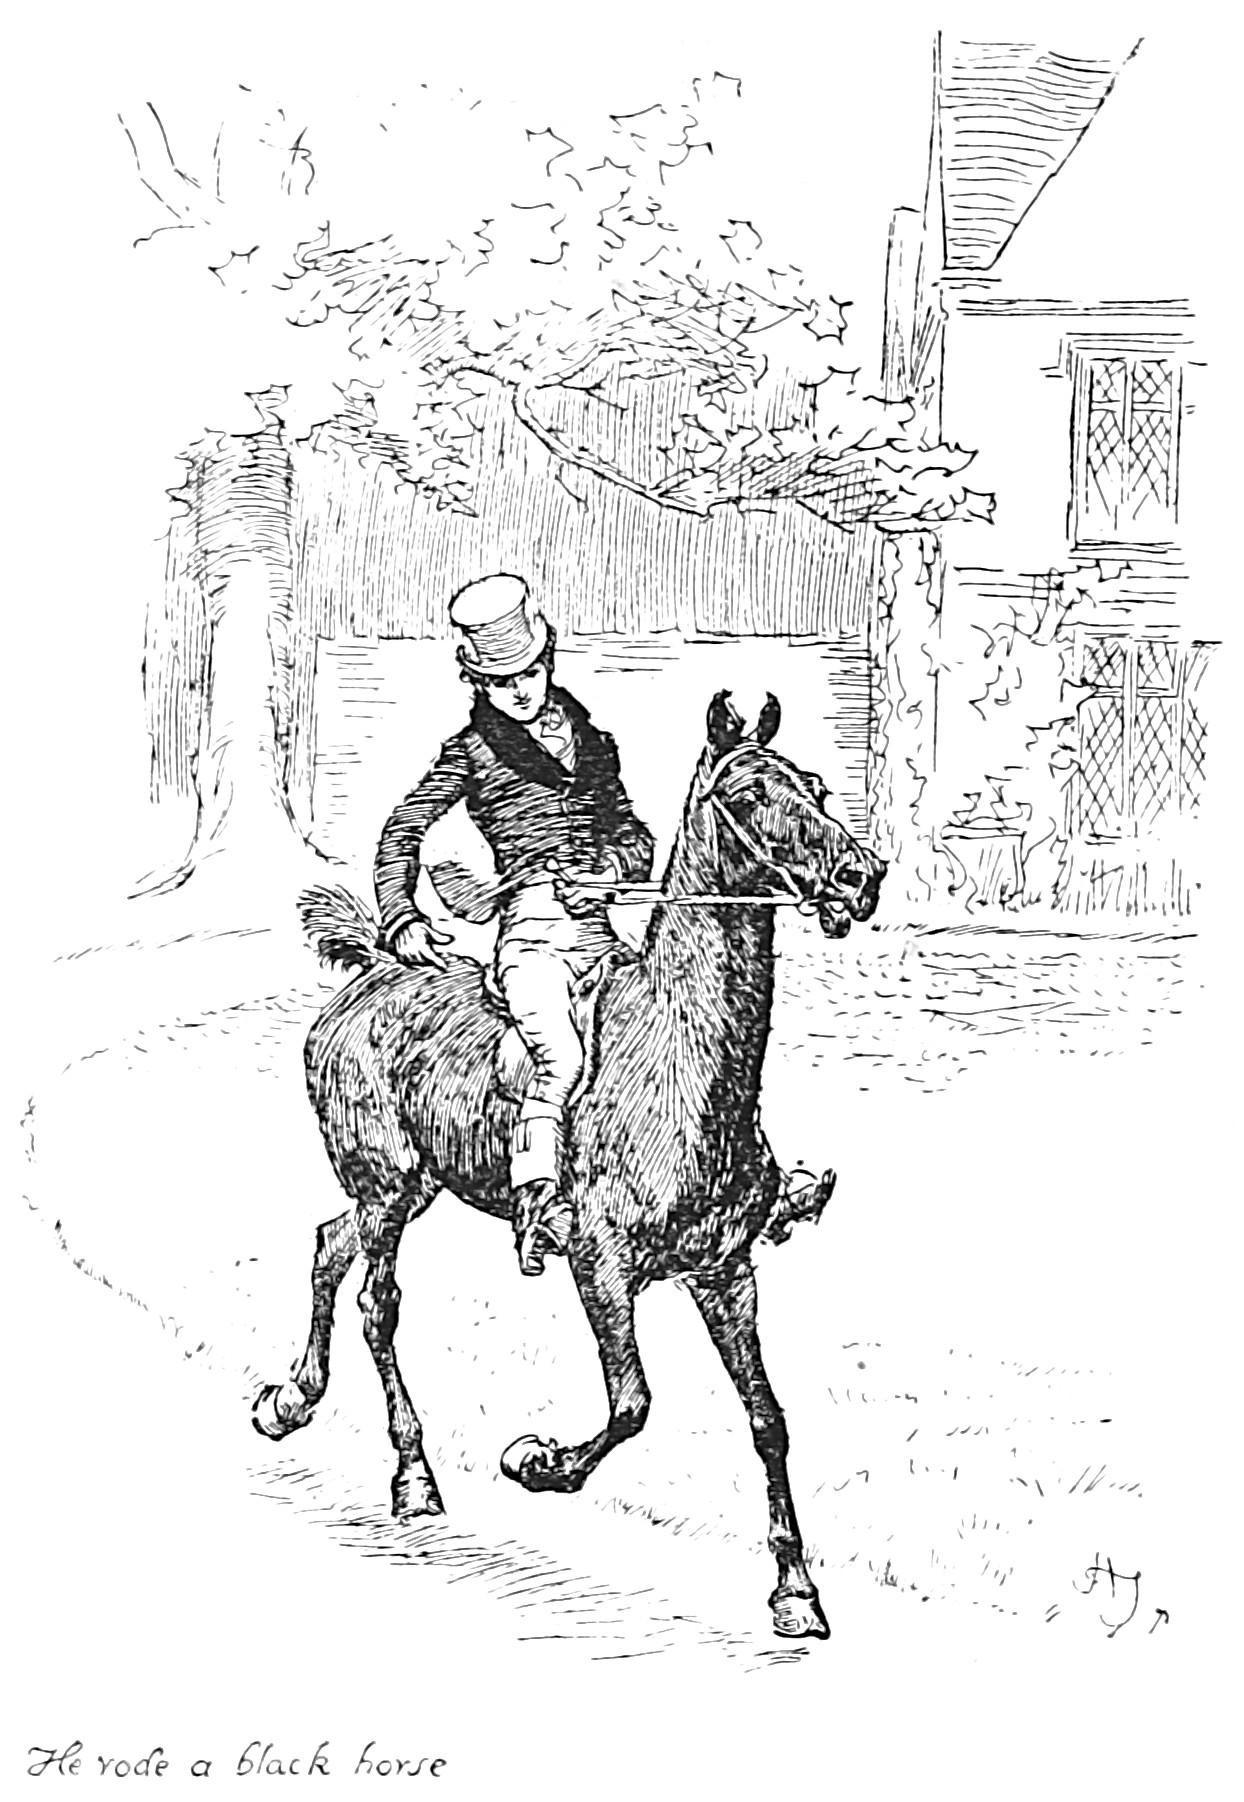
\includegraphics[width=.7\linewidth]{3blackhorse}
		\captionlistentry{He rode a black horse}
	\end{figure}


\lettrine[lines=6,image=true]{initials/chap3n}{ot} all that Mrs Bennet, however, with the assistance of her five daughters, could ask on the subject, was sufficient to draw from her husband any satisfactory description of Mr Bingley. They attacked him in various ways, with barefaced questions, ingenious suppositions, and distant surmises; but he eluded the skill of them all; and they were at last obliged to accept the second-hand intelligence of their neighbour, Lady Lucas. Her report was highly favourable. Sir William had been delighted with him. He was quite young, wonderfully handsome, extremely agreeable, and, to crown the whole, he meant to be at the next assembly with a large party. Nothing could be more delightful! To be fond of dancing was a certain step towards falling in love; and very lively hopes of Mr Bingley's heart were entertained.

<If I can but see one of my daughters happily settled at Netherfield,> said Mrs Bennet to her husband, <and all the others equally well married, I shall have nothing to wish for.>

In a few days Mr Bingley returned Mr Bennet's visit, and sat about ten minutes with him in his library. He had entertained hopes of being admitted to a sight of the young ladies, of whose beauty he had heard much; but he saw only the father. The ladies were somewhat more fortunate, for they had the advantage of ascertaining, from an upper window, that he wore a blue coat and rode a black horse.

\begin{figure}[tbh]
\centering
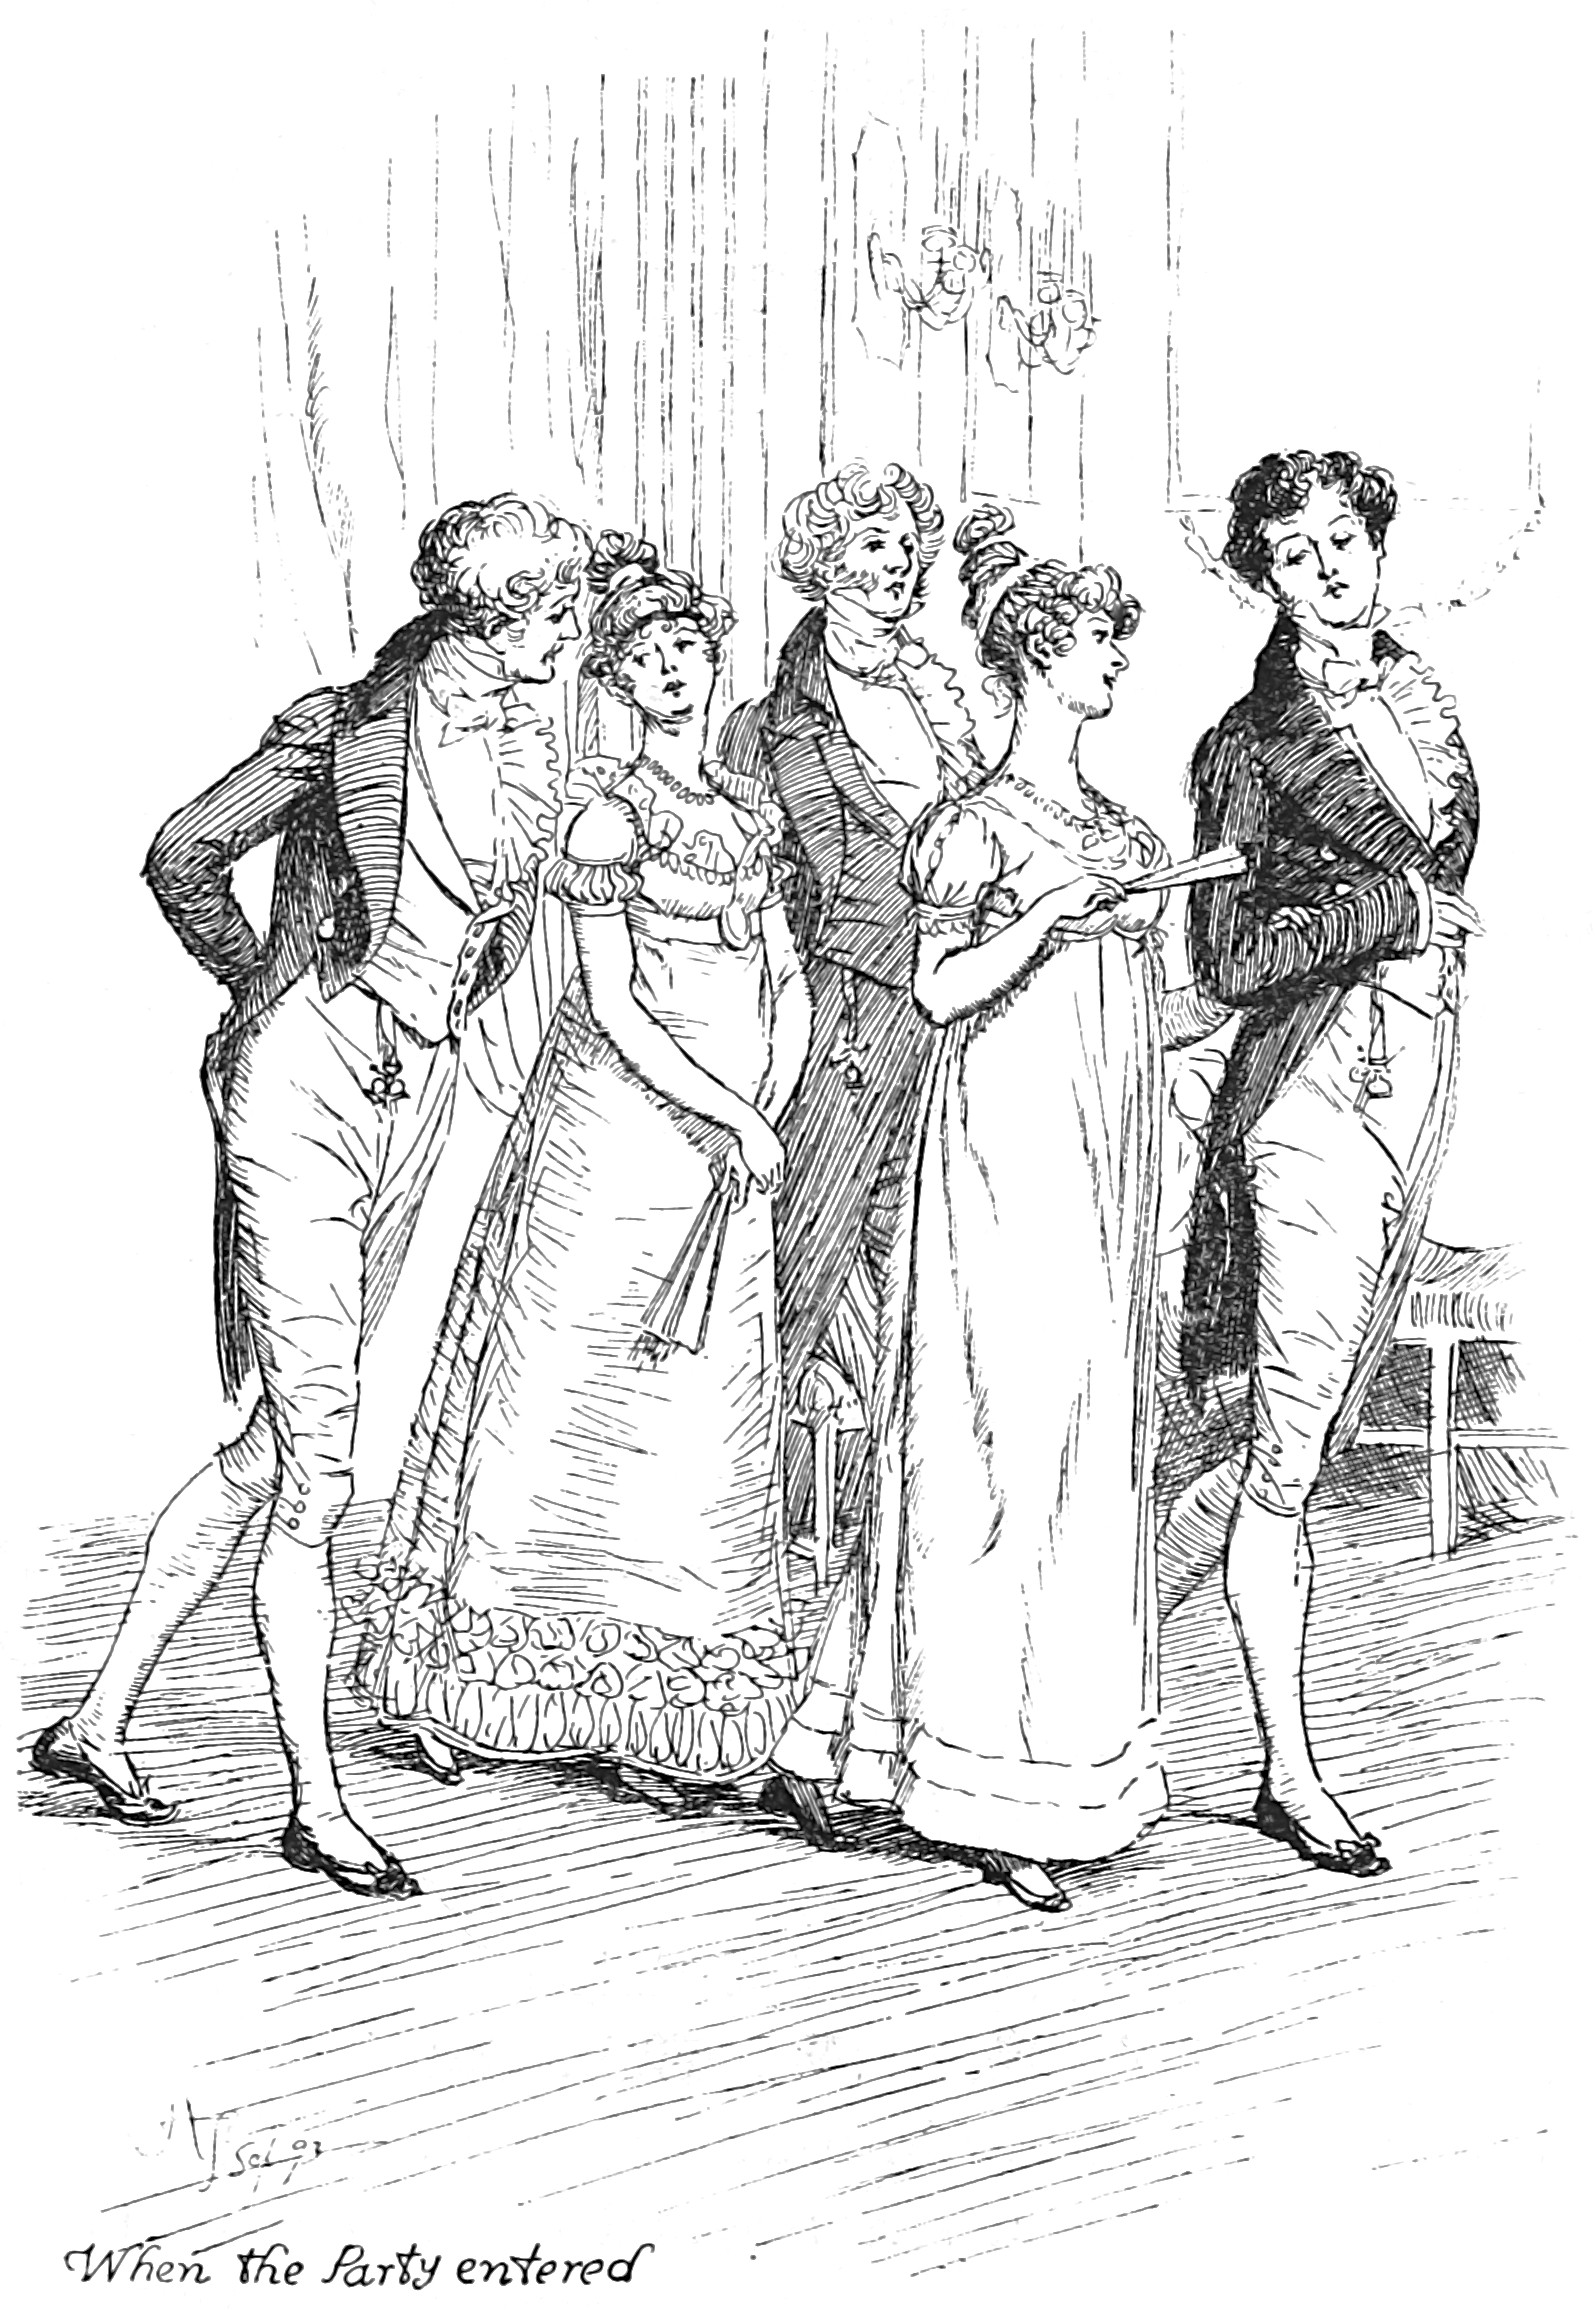
\includegraphics[width=.7\linewidth]{3partyentered}
\captionlistentry{When the party entered}
\end{figure}

An invitation to dinner was soon afterwards despatched; and already had Mrs Bennet planned the courses that were to do credit to her housekeeping, when an answer arrived which deferred it all. Mr Bingley was obliged to be in town the following day, and consequently unable to accept the honour of their invitation, etc. Mrs Bennet was quite disconcerted. She could not imagine what business he could have in town so soon after his arrival in Hertfordshire; and she began to fear that he might always be flying about from one place to another, and never settled at Netherfield as he ought to be. Lady Lucas quieted her fears a little by starting the idea of his being gone to London only to get a large party for the ball; and a report soon followed that Mr Bingley was to bring twelve ladies and seven gentlemen with him to the assembly. The girls grieved over such a number of ladies; but were comforted the day before the ball by hearing that, instead of twelve, he had brought only six with him from London, his five sisters and a cousin. And when the party entered the assembly-room, it consisted of only five altogether: Mr Bingley, his two sisters, the husband of the eldest, and another young man.

Mr Bingley was good-looking and gentlemanlike: he had a pleasant countenance, and easy, unaffected manners. His sisters were fine women, with an air of decided fashion. His brother-in-law, Mr Hurst, merely looked the gentleman; but his friend Mr Darcy soon drew the attention of the room by his fine, tall person, handsome features, noble mien, and the report, which was in general circulation within five minutes after his entrance, of his having ten thousand a year. The gentlemen pronounced him to be a fine figure of a man, the ladies declared he was much handsomer than Mr Bingley, and he was looked at with great admiration for about half the evening, till his manners gave a disgust which turned the tide of his popularity; for he was discovered to be proud, to be above his company, and above being pleased; and not all his large estate in Derbyshire could save him from having a most forbidding, disagreeable countenance, and being unworthy to be compared with his friend.

Mr Bingley had soon made himself acquainted with all the principal people in the room: he was lively and unreserved, danced every dance, was angry that the ball closed so early, and talked of giving one himself at Netherfield. Such amiable qualities must speak for themselves. What a contrast between him and his friend! Mr Darcy danced only once with Mrs Hurst and once with Miss Bingley, declined being introduced to any other lady, and spent the rest of the evening in walking about the room, speaking occasionally to one of his own party. His character was decided. He was the proudest, most disagreeable man in the world, and everybody hoped that he would never come there again. Amongst the most violent against him was Mrs Bennet, whose dislike of his general behaviour was sharpened into particular resentment by his having slighted one of her daughters.



Elizabeth Bennet had been obliged, by the scarcity of gentlemen, to sit down for two dances; and during part of that time, Mr Darcy had been standing near enough for her to overhear a conversation between him and Mr Bingley, who came from the dance for a few minutes to press his friend to join it.

<Come, Darcy,> said he, <I must have you dance. I hate to see you standing about by yourself in this stupid manner. You had much better dance.>

<I certainly shall not. You know how I detest it, unless I am particularly acquainted with my partner. At such an assembly as this, it would be insupportable. Your sisters are engaged, and there is not another woman in the room whom it would not be a punishment to me to stand up with.>

<I would not be so fastidious as you are,> cried Bingley, <for a kingdom! Upon my honour, I never met with so many pleasant girls in my life as I have this evening; and there are several of them, you see, uncommonly pretty.>

<\textit{You} are dancing with the only handsome girl in the room,> said Mr Darcy, looking at the eldest Miss Bennet.

<Oh, she is the most beautiful creature I ever beheld! But there is one of her sisters sitting down just behind you, who is very pretty, and I dare say very agreeable. Do let me ask my partner to introduce you.>

\begin{figure}[tbh]
\centering
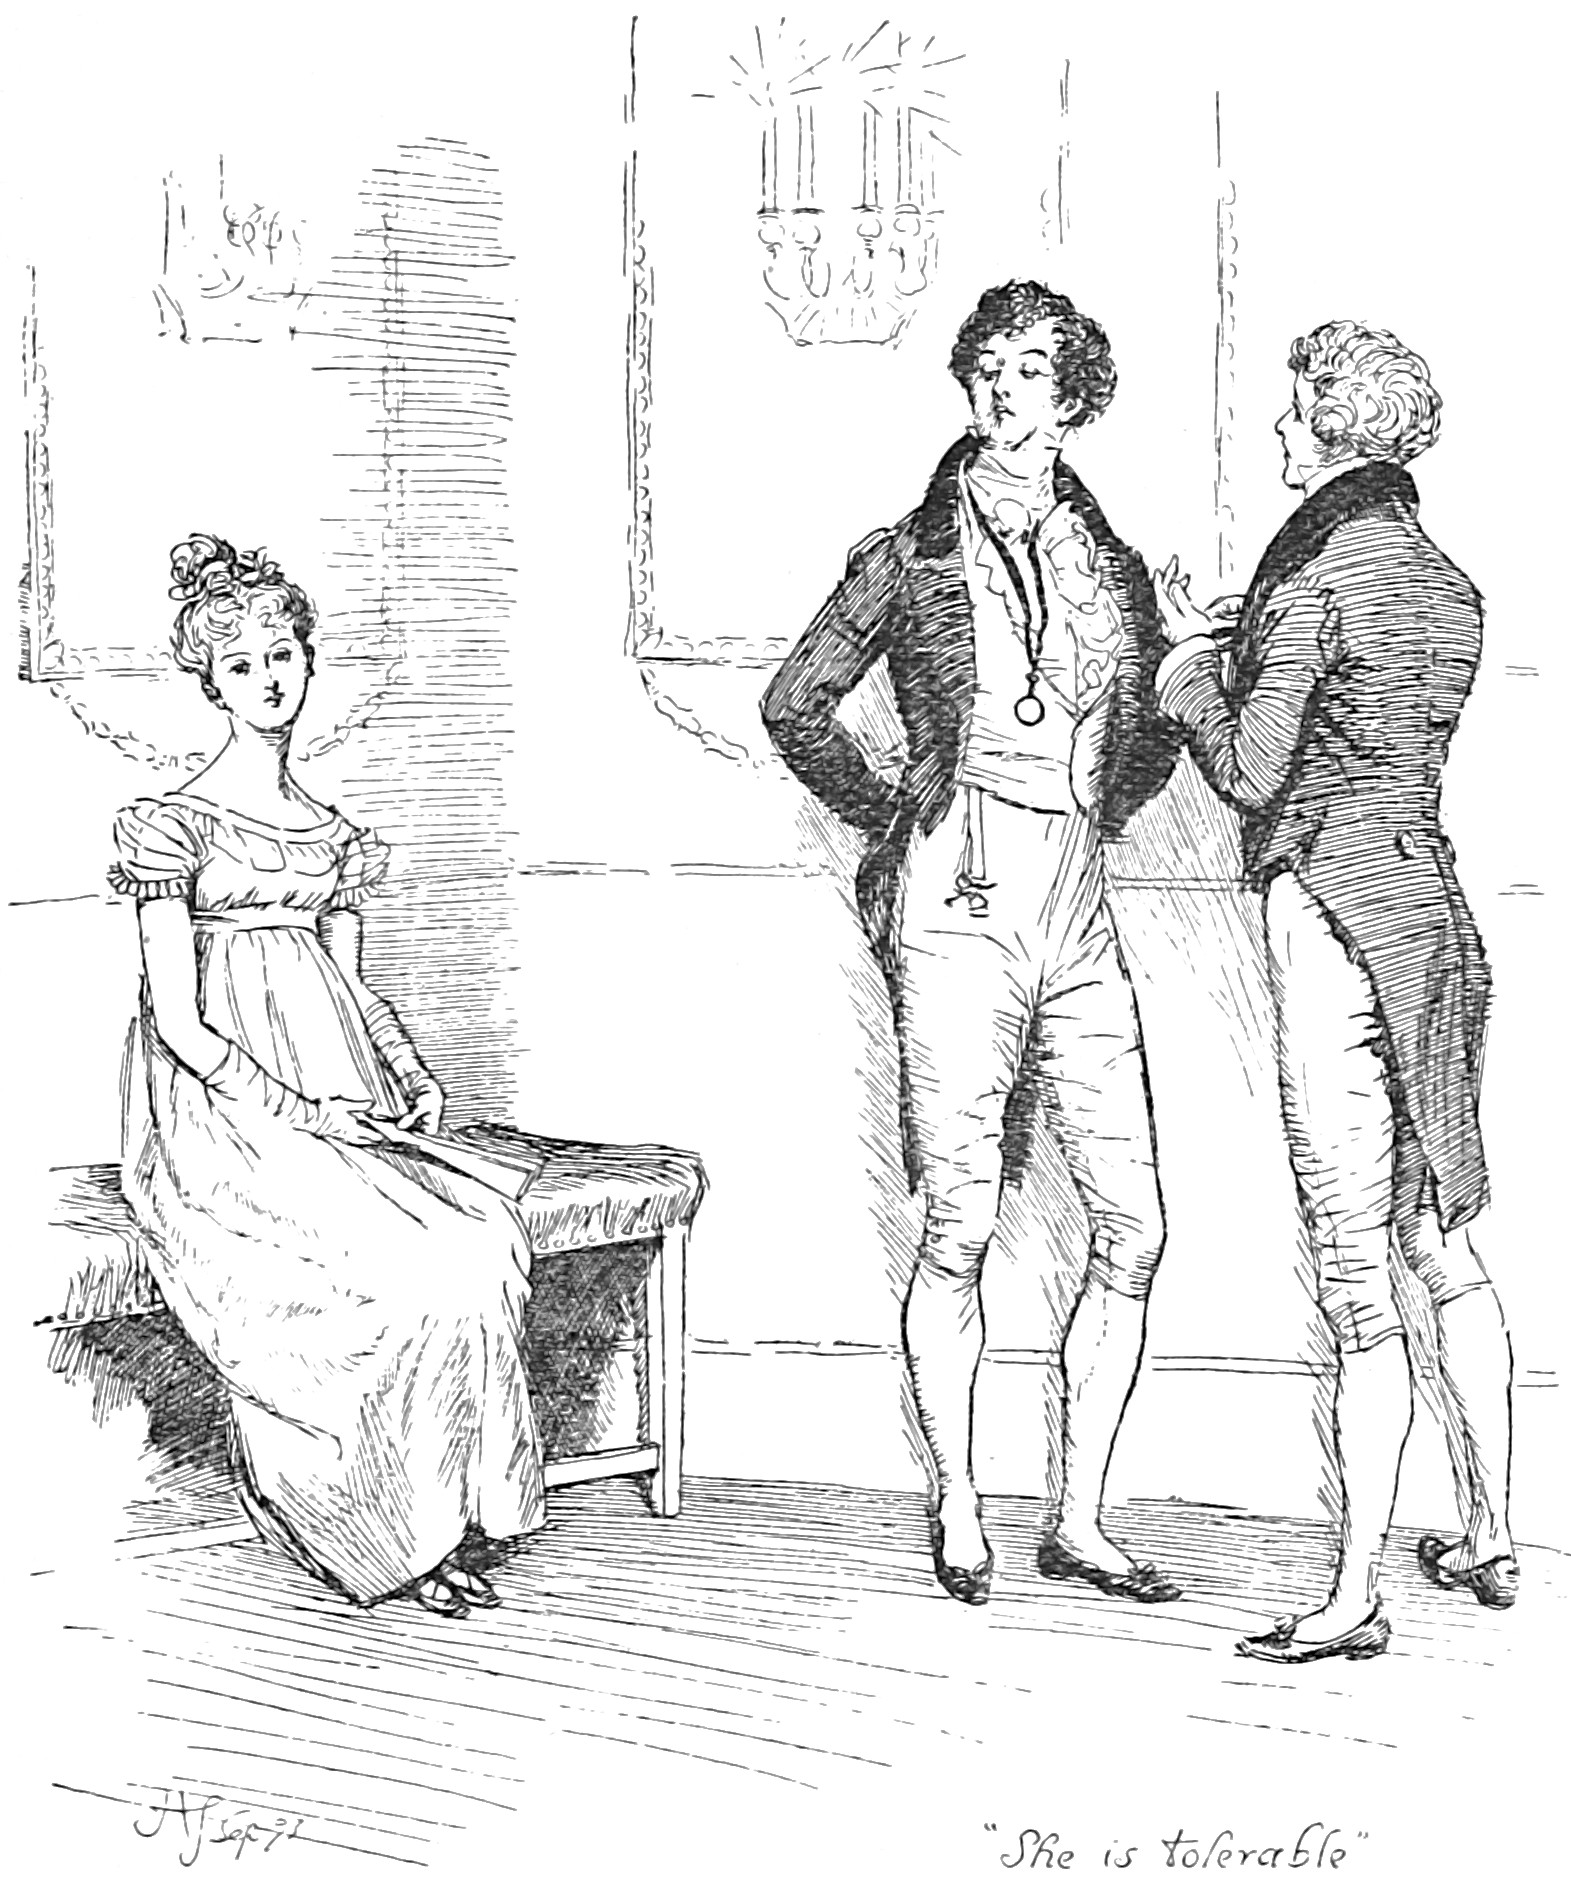
\includegraphics[width=.8\linewidth]{3tolerable}
\captionlistentry{<She is tolerable>}
\end{figure}

<Which do you mean?> and turning round, he looked for a moment at Elizabeth, till, catching her eye, he withdrew his own, and coldly said, <She is tolerable: but not handsome enough to tempt \textit{me}; and I am in no humour at present to give consequence to young ladies who are slighted by other men. You had better return to your partner and enjoy her smiles, for you are wasting your time with me.>



Mr Bingley followed his advice. Mr Darcy walked off; and Elizabeth remained with no very cordial feelings towards him. She told the story, however, with great spirit among her friends; for she had a lively, playful disposition, which delighted in anything ridiculous.

The evening altogether passed off pleasantly to the whole family. Mrs Bennet had seen her eldest daughter much admired by the Netherfield party. Mr Bingley had danced with her twice, and she had been distinguished by his sisters. Jane was as much gratified by this as her mother could be, though in a quieter way. Elizabeth felt Jane's pleasure. Mary had heard herself mentioned to Miss Bingley as the most accomplished girl in the neighbourhood; and Catherine and Lydia had been fortunate enough to be never without partners, which was all that they had yet learnt to care for at a ball. They returned, therefore, in good spirits to Longbourn, the village where they lived, and of which they were the principal inhabitants. They found Mr Bennet still up. With a book, he was regardless of time; and on the present occasion he had a good deal of curiosity as to the event of an evening which had raised such splendid expectations. He had rather hoped that all his wife's views on the stranger would be disappointed; but he soon found that he had a very different story to hear.

<Oh, my dear Mr Bennet,> as she entered the room, <we have had a most delightful evening, a most excellent ball. I wish you had been there. Jane was so admired, nothing could be like it. Everybody said how well she looked; and Mr Bingley thought her quite beautiful, and danced with her twice. Only think of \textit{that}, my dear: he actually danced with her twice; and she was the only creature in the room that he asked a second time. First of all, he asked Miss Lucas. I was so vexed to see him stand up with her; but, however, he did not admire her at all; indeed, nobody can, you know; and he seemed quite struck with Jane as she was going down the dance. So he inquired who she was, and got introduced, and asked her for the two next. Then, the two third he danced with Miss King, and the two fourth with Maria Lucas, and the two fifth with Jane again, and the two sixth with Lizzy, and the \textit{Boulanger}\longdash>

<If he had had any compassion for \textit{me},> cried her husband impatiently, <he would not have danced half so much! For God's sake, say no more of his partners. O that he had sprained his ancle in the first dance!>

<Oh, my dear,> continued Mrs Bennet, <I am quite delighted with him. He is so excessively handsome! and his sisters are charming women. I never in my life saw anything more elegant than their dresses. I dare say the lace upon Mrs Hurst's gown\longdash>

Here she was interrupted again. Mr Bennet protested against any description of finery. She was therefore obliged to seek another branch of the subject, and related, with much bitterness of spirit, and some exaggeration, the shocking rudeness of Mr Darcy.

<But I can assure you,> she added, <that Lizzy does not lose much by not suiting \textit{his} fancy; for he is a most disagreeable, horrid man, not at all worth pleasing. So high and so conceited, that there was no enduring him! He walked here, and he walked there, fancying himself so very great! Not handsome enough to dance with! I wish you had been there, my dear, to have given him one of your set-downs. I quite detest the man.>

%!TeX root=../emmatop.tex
\chapter[Chapter \thechapter]{}
\lettrine[lines=4,lraise=0.3]{H}{arriet} Smith's intimacy at Hartfield was soon a settled thing. Quick and decided in her ways, Emma lost no time in inviting, encouraging, and telling her to come very often; and as their acquaintance increased, so did their satisfaction in each other. As a walking companion, Emma had very early foreseen how useful she might find her. In that respect Mrs Weston's loss had been important. Her father never went beyond the shrubbery, where two divisions of the ground sufficed him for his long walk, or his short, as the year varied; and since Mrs Weston's marriage her exercise had been too much confined. She had ventured once alone to Randalls, but it was not pleasant; and a Harriet Smith, therefore, one whom she could summon at any time to a walk, would be a valuable addition to her privileges. But in every respect, as she saw more of her, she approved her, and was confirmed in all her kind designs.

Harriet certainly was not clever, but she had a sweet, docile, grateful disposition, was totally free from conceit, and only desiring to be guided by any one she looked up to. Her early attachment to herself was very amiable; and her inclination for good company, and power of appreciating what was elegant and clever, shewed that there was no want of taste, though strength of understanding must not be expected. Altogether she was quite convinced of Harriet Smith's being exactly the young friend she wanted—exactly the something which her home required. Such a friend as Mrs Weston was out of the question. Two such could never be granted. Two such she did not want. It was quite a different sort of thing, a sentiment distinct and independent. Mrs Weston was the object of a regard which had its basis in gratitude and esteem. Harriet would be loved as one to whom she could be useful. For Mrs Weston there was nothing to be done; for Harriet every thing.

Her first attempts at usefulness were in an endeavour to find out who were the parents, but Harriet could not tell. She was ready to tell every thing in her power, but on this subject questions were vain. Emma was obliged to fancy what she liked—but she could never believe that in the same situation \textit{she} should not have discovered the truth. Harriet had no penetration. She had been satisfied to hear and believe just what Mrs Goddard chose to tell her; and looked no farther.

Mrs Goddard, and the teachers, and the girls and the affairs of the school in general, formed naturally a great part of the conversation—and but for her acquaintance with the Martins of Abbey-Mill Farm, it must have been the whole. But the Martins occupied her thoughts a good deal; she had spent two very happy months with them, and now loved to talk of the pleasures of her visit, and describe the many comforts and wonders of the place. Emma encouraged her talkativeness—amused by such a picture of another set of beings, and enjoying the youthful simplicity which could speak with so much exultation of Mrs Martin's having »\textit{two} parlours, two very good parlours, indeed; one of them quite as large as Mrs Goddard's drawing-room; and of her having an upper maid who had lived five-and-twenty years with her; and of their having eight cows, two of them Alderneys, and one a little Welch cow, a very pretty little Welch cow indeed; and of Mrs Martin's saying as she was so fond of it, it should be called \textit{her} cow; and of their having a very handsome summer-house in their garden, where some day next year they were all to drink tea:—a very handsome summer-house, large enough to hold a dozen people.«

For some time she was amused, without thinking beyond the immediate cause; but as she came to understand the family better, other feelings arose. She had taken up a wrong idea, fancying it was a mother and daughter, a son and son's wife, who all lived together; but when it appeared that the Mr Martin, who bore a part in the narrative, and was always mentioned with approbation for his great good-nature in doing something or other, was a single man; that there was no young Mrs Martin, no wife in the case; she did suspect danger to her poor little friend from all this hospitality and kindness, and that, if she were not taken care of, she might be required to sink herself forever.

With this inspiriting notion, her questions increased in number and meaning; and she particularly led Harriet to talk more of Mr Martin, and there was evidently no dislike to it. Harriet was very ready to speak of the share he had had in their moonlight walks and merry evening games; and dwelt a good deal upon his being so very good-humoured and obliging. He had gone three miles round one day in order to bring her some walnuts, because she had said how fond she was of them, and in every thing else he was so very obliging. He had his shepherd's son into the parlour one night on purpose to sing to her. She was very fond of singing. He could sing a little himself. She believed he was very clever, and understood every thing. He had a very fine flock, and, while she was with them, he had been bid more for his wool than any body in the country. She believed every body spoke well of him. His mother and sisters were very fond of him. Mrs Martin had told her one day (and there was a blush as she said it,) that it was impossible for any body to be a better son, and therefore she was sure, whenever he married, he would make a good husband. Not that she \textit{wanted} him to marry. She was in no hurry at all.

»Well done, Mrs Martin!« thought Emma. »You know what you are about.«

»And when she had come away, Mrs Martin was so very kind as to send Mrs Goddard a beautiful goose—the finest goose Mrs Goddard had ever seen. Mrs Goddard had dressed it on a Sunday, and asked all the three teachers, Miss Nash, and Miss Prince, and Miss Richardson, to sup with her.«

»Mr Martin, I suppose, is not a man of information beyond the line of his own business? He does not read?«

»Oh yes!—that is, no—I do not know—but I believe he has read a good deal—but not what you would think any thing of. He reads the \textit{Agricultural Reports}, and some other books that lay in one of the window seats—but he reads all \textit{them} to himself. But sometimes of an evening, before we went to cards, he would read something aloud out of the \textit{Elegant Extracts}, very entertaining. And I know he has read \textit{The Vicar of Wakefield}. He never read \textit{The Romance of the Forest}, nor \textit{The Children of the Abbey}. He had never heard of such books before I mentioned them, but he is determined to get them now as soon as ever he can.«

The next question was—

»What sort of looking man is Mr Martin?«

»Oh! not handsome—not at all handsome. I thought him very plain at first, but I do not think him so plain now. One does not, you know, after a time. But did you never see him? He is in Highbury every now and then, and he is sure to ride through every week in his way to Kingston. He has passed you very often.«

»That may be, and I may have seen him fifty times, but without having any idea of his name. A young farmer, whether on horseback or on foot, is the very last sort of person to raise my curiosity. The yeomanry are precisely the order of people with whom I feel I can have nothing to do. A degree or two lower, and a creditable appearance might interest me; I might hope to be useful to their families in some way or other. But a farmer can need none of my help, and is, therefore, in one sense, as much above my notice as in every other he is below it.«

»To be sure. Oh yes! It is not likely you should ever have observed him; but he knows you very well indeed—I mean by sight.«

»I have no doubt of his being a very respectable young man. I know, indeed, that he is so, and, as such, wish him well. What do you imagine his age to be?«

»He was four-and-twenty the 8th of last June, and my birthday is the 23rd just a fortnight and a day's difference—which is very odd.«

»Only four-and-twenty. That is too young to settle. His mother is perfectly right not to be in a hurry. They seem very comfortable as they are, and if she were to take any pains to marry him, she would probably repent it. Six years hence, if he could meet with a good sort of young woman in the same rank as his own, with a little money, it might be very desirable.«

»Six years hence! Dear Miss Woodhouse, he would be thirty years old!«

»Well, and that is as early as most men can afford to marry, who are not born to an independence. Mr Martin, I imagine, has his fortune entirely to make—cannot be at all beforehand with the world. Whatever money he might come into when his father died, whatever his share of the family property, it is, I dare say, all afloat, all employed in his stock, and so forth; and though, with diligence and good luck, he may be rich in time, it is next to impossible that he should have realised any thing yet.«

»To be sure, so it is. But they live very comfortably. They have no indoors man, else they do not want for any thing; and Mrs Martin talks of taking a boy another year.«

»I wish you may not get into a scrape, Harriet, whenever he does marry;—I mean, as to being acquainted with his wife—for though his sisters, from a superior education, are not to be altogether objected to, it does not follow that he might marry any body at all fit for you to notice. The misfortune of your birth ought to make you particularly careful as to your associates. There can be no doubt of your being a gentleman's daughter, and you must support your claim to that station by every thing within your own power, or there will be plenty of people who would take pleasure in degrading you.«

»Yes, to be sure, I suppose there are. But while I visit at Hartfield, and you are so kind to me, Miss Woodhouse, I am not afraid of what any body can do.«

»You understand the force of influence pretty well, Harriet; but I would have you so firmly established in good society, as to be independent even of Hartfield and Miss Woodhouse. I want to see you permanently well connected, and to that end it will be advisable to have as few odd acquaintance as may be; and, therefore, I say that if you should still be in this country when Mr Martin marries, I wish you may not be drawn in by your intimacy with the sisters, to be acquainted with the wife, who will probably be some mere farmer's daughter, without education.«

»To be sure. Yes. Not that I think Mr Martin would ever marry any body but what had had some education—and been very well brought up. However, I do not mean to set up my opinion against yours—and I am sure I shall not wish for the acquaintance of his wife. I shall always have a great regard for the Miss Martins, especially Elizabeth, and should be very sorry to give them up, for they are quite as well educated as me. But if he marries a very ignorant, vulgar woman, certainly I had better not visit her, if I can help it.«

Emma watched her through the fluctuations of this speech, and saw no alarming symptoms of love. The young man had been the first admirer, but she trusted there was no other hold, and that there would be no serious difficulty, on Harriet's side, to oppose any friendly arrangement of her own.

\begin{figure}[tbph]
\centering
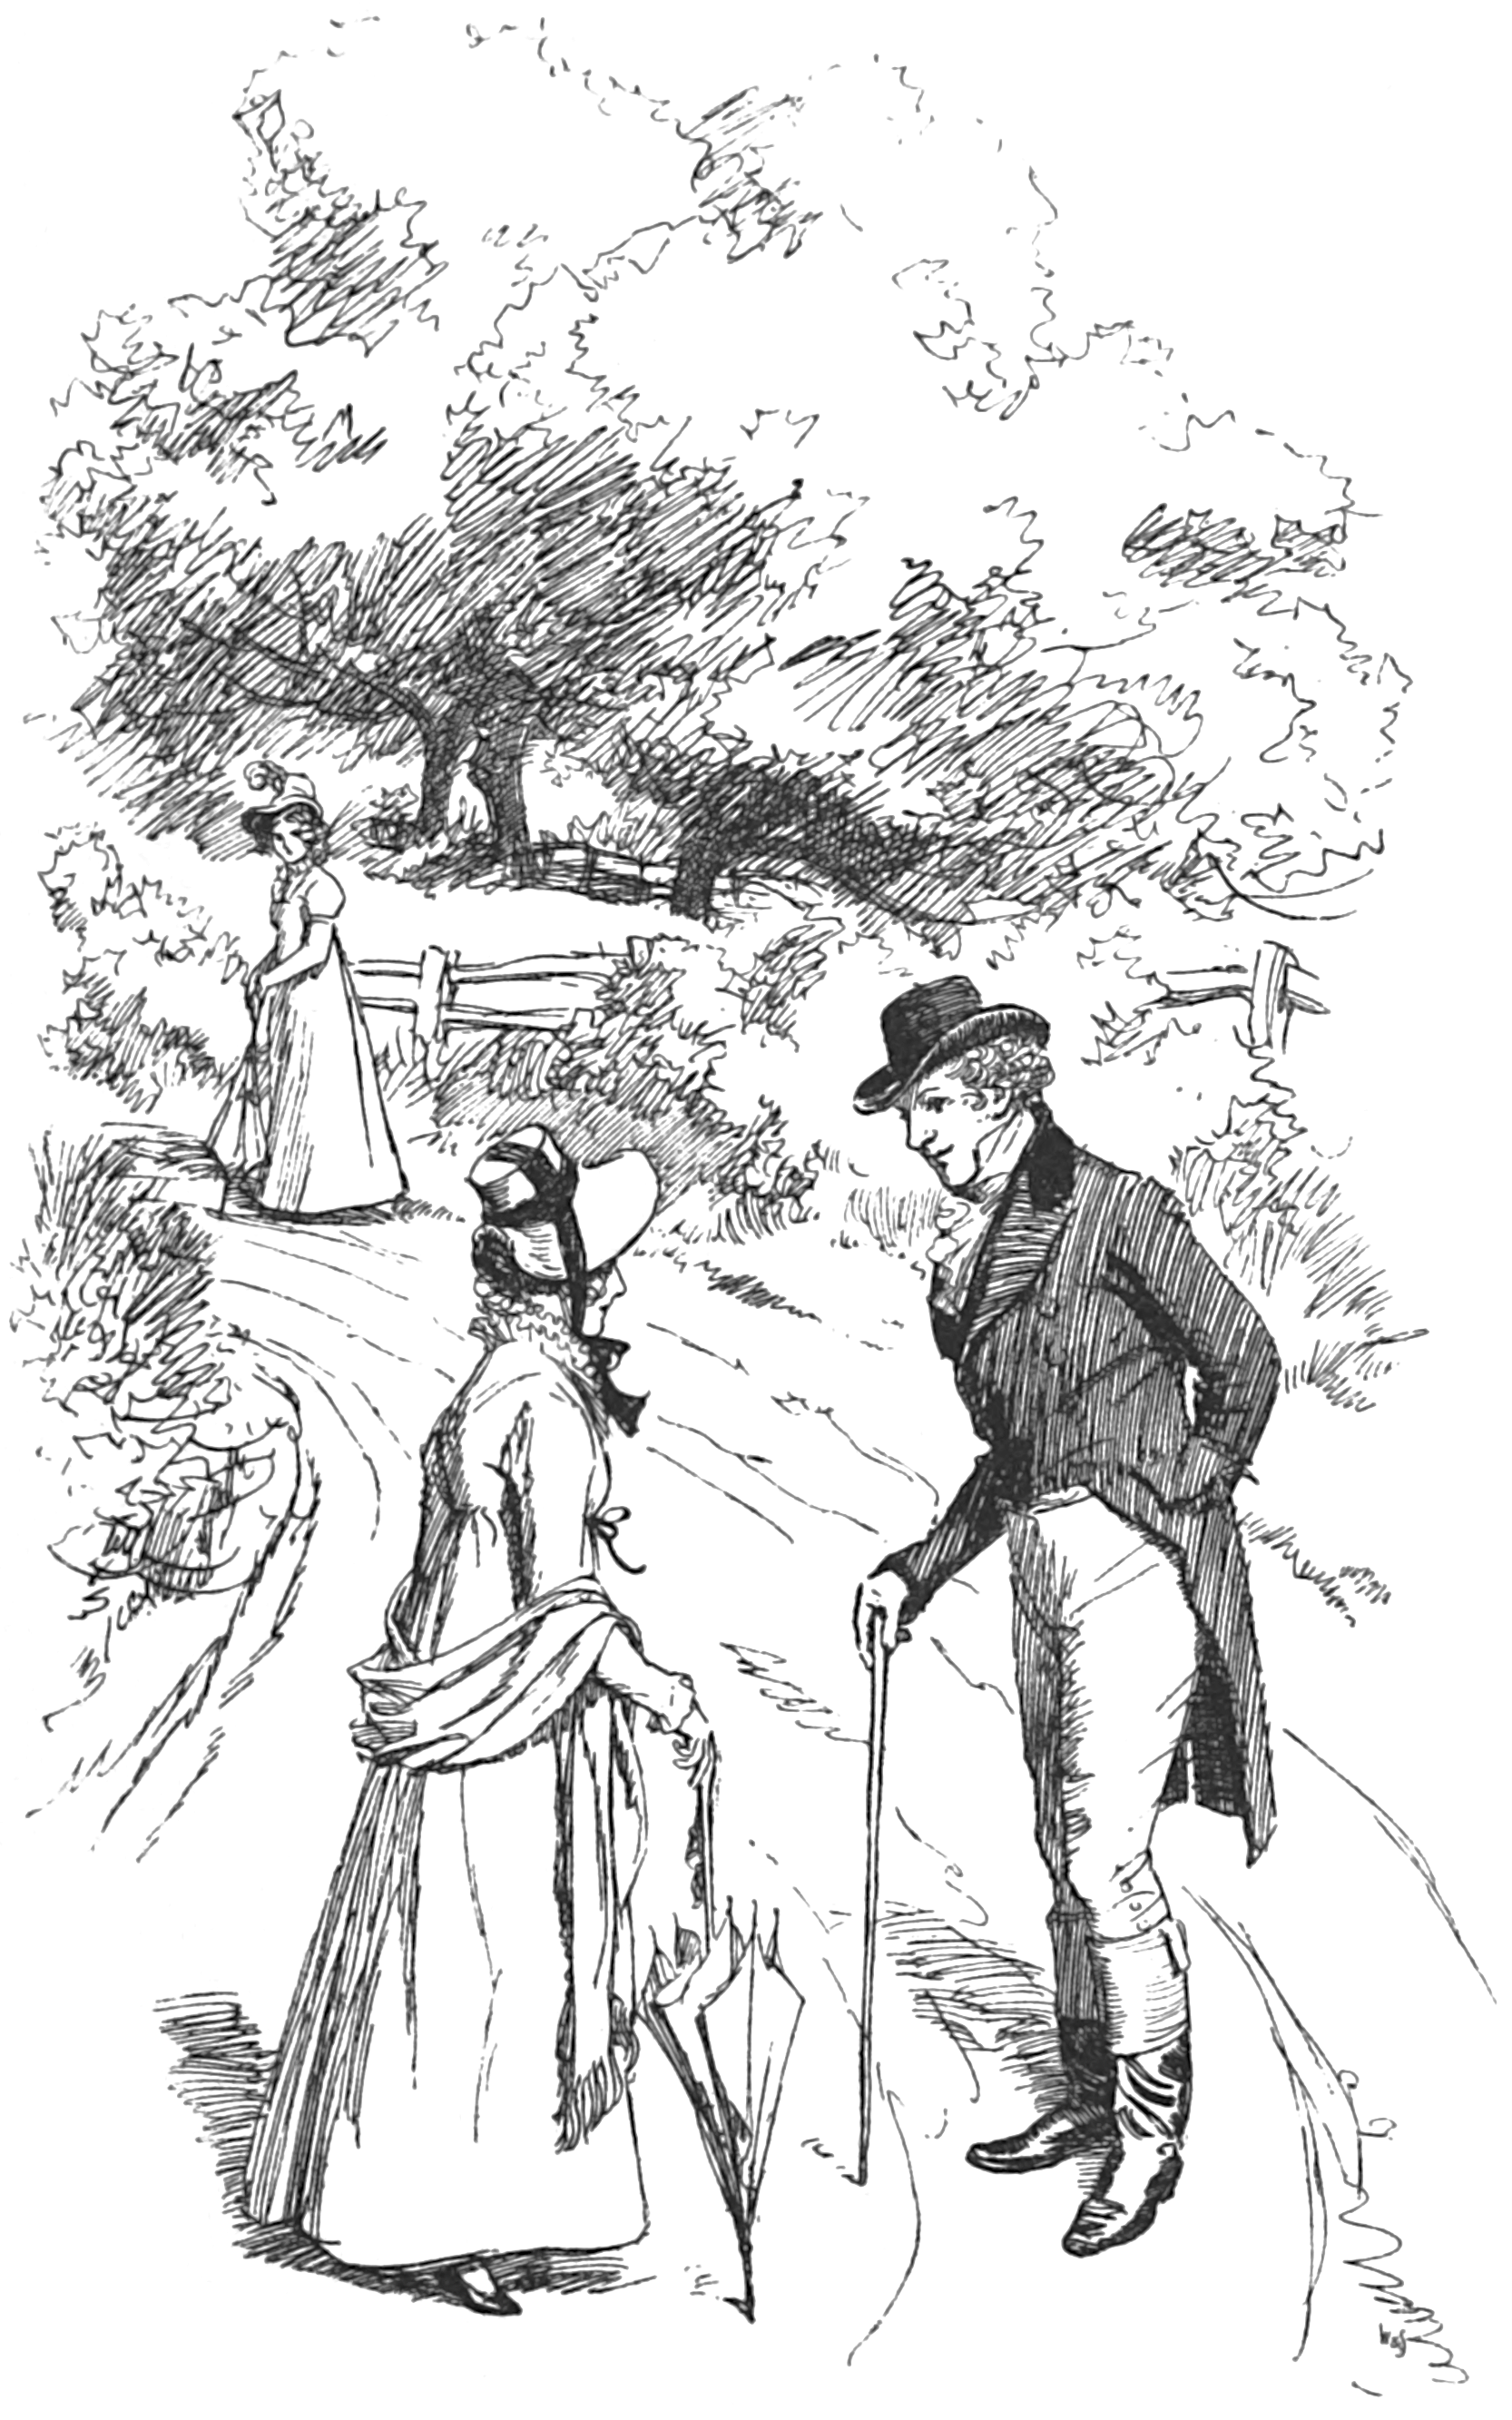
\includegraphics[width=.8\linewidth]{4notsorry}
\caption{Emma was not sorry to have such an opportunity of survey}
\end{figure}

They met Mr Martin the very next day, as they were walking on the Donwell road. He was on foot, and after looking very respectfully at her, looked with most unfeigned satisfaction at her companion. Emma was not sorry to have such an opportunity of survey; and walking a few yards forward, while they talked together, soon made her quick eye sufficiently acquainted with Mr Robert Martin. His appearance was very neat, and he looked like a sensible young man, but his person had no other advantage; and when he came to be contrasted with gentlemen, she thought he must lose all the ground he had gained in Harriet's inclination. Harriet was not insensible of manner; she had voluntarily noticed her father's gentleness with admiration as well as wonder. Mr Martin looked as if he did not know what manner was.

They remained but a few minutes together, as Miss Woodhouse must not be kept waiting; and Harriet then came running to her with a smiling face, and in a flutter of spirits, which Miss Woodhouse hoped very soon to compose.

»Only think of our happening to meet him!—How very odd! It was quite a chance, he said, that he had not gone round by Randalls. He did not think we ever walked this road. He thought we walked towards Randalls most days. He has not been able to get the Romance of the Forest yet. He was so busy the last time he was at Kingston that he quite forgot it, but he goes again to-morrow. So very odd we should happen to meet! Well, Miss Woodhouse, is he like what you expected? What do you think of him? Do you think him so very plain?«

»He is very plain, undoubtedly—remarkably plain:—but that is nothing compared with his entire want of gentility. I had no right to expect much, and I did not expect much; but I had no idea that he could be so very clownish, so totally without air. I had imagined him, I confess, a degree or two nearer gentility.«

»To be sure,« said Harriet, in a mortified voice, »he is not so genteel as real gentlemen.«

»I think, Harriet, since your acquaintance with us, you have been repeatedly in the company of some such very real gentlemen, that you must yourself be struck with the difference in Mr Martin. At Hartfield, you have had very good specimens of well educated, well bred men. I should be surprized if, after seeing them, you could be in company with Mr Martin again without perceiving him to be a very inferior creature—and rather wondering at yourself for having ever thought him at all agreeable before. Do not you begin to feel that now? Were not you struck? I am sure you must have been struck by his awkward look and abrupt manner, and the uncouthness of a voice which I heard to be wholly unmodulated as I stood here.«

»Certainly, he is not like Mr Knightley. He has not such a fine air and way of walking as Mr Knightley. I see the difference plain enough. But Mr Knightley is so very fine a man!«

»Mr Knightley's air is so remarkably good that it is not fair to compare Mr Martin with \textit{him}. You might not see one in a hundred with \textit{gentleman} so plainly written as in Mr Knightley. But he is not the only gentleman you have been lately used to. What say you to Mr Weston and Mr Elton? Compare Mr Martin with either of \textit{them}. Compare their manner of carrying themselves; of walking; of speaking; of being silent. You must see the difference.«

»Oh yes!—there is a great difference. But Mr Weston is almost an old man. Mr Weston must be between forty and fifty.«

»Which makes his good manners the more valuable. The older a person grows, Harriet, the more important it is that their manners should not be bad; the more glaring and disgusting any loudness, or coarseness, or awkwardness becomes. What is passable in youth is detestable in later age. Mr Martin is now awkward and abrupt; what will he be at Mr Weston's time of life?«

»There is no saying, indeed,« replied Harriet rather solemnly.

»But there may be pretty good guessing. He will be a completely gross, vulgar farmer, totally inattentive to appearances, and thinking of nothing but profit and loss.«

»Will he, indeed? That will be very bad.«

»How much his business engrosses him already is very plain from the circumstance of his forgetting to inquire for the book you recommended. He was a great deal too full of the market to think of any thing else—which is just as it should be, for a thriving man. What has he to do with books? And I have no doubt that he \textit{will} thrive, and be a very rich man in time—and his being illiterate and coarse need not disturb \textit{us}.«

»I wonder he did not remember the book«—was all Harriet's answer, and spoken with a degree of grave displeasure which Emma thought might be safely left to itself. She, therefore, said no more for some time. Her next beginning was,

»In one respect, perhaps, Mr Elton's manners are superior to Mr Knightley's or Mr Weston's. They have more gentleness. They might be more safely held up as a pattern. There is an openness, a quickness, almost a bluntness in Mr Weston, which every body likes in \textit{him}, because there is so much good-humour with it—but that would not do to be copied. Neither would Mr Knightley's downright, decided, commanding sort of manner, though it suits \textit{him} very well; his figure, and look, and situation in life seem to allow it; but if any young man were to set about copying him, he would not be sufferable. On the contrary, I think a young man might be very safely recommended to take Mr Elton as a model. Mr Elton is good-humoured, cheerful, obliging, and gentle. He seems to me to be grown particularly gentle of late. I do not know whether he has any design of ingratiating himself with either of us, Harriet, by additional softness, but it strikes me that his manners are softer than they used to be. If he means any thing, it must be to please you. Did not I tell you what he said of you the other day?«

She then repeated some warm personal praise which she had drawn from Mr Elton, and now did full justice to; and Harriet blushed and smiled, and said she had always thought Mr Elton very agreeable.

Mr Elton was the very person fixed on by Emma for driving the young farmer out of Harriet's head. She thought it would be an excellent match; and only too palpably desirable, natural, and probable, for her to have much merit in planning it. She feared it was what every body else must think of and predict. It was not likely, however, that any body should have equalled her in the date of the plan, as it had entered her brain during the very first evening of Harriet's coming to Hartfield. The longer she considered it, the greater was her sense of its expediency. Mr Elton's situation was most suitable, quite the gentleman himself, and without low connexions; at the same time, not of any family that could fairly object to the doubtful birth of Harriet. He had a comfortable home for her, and Emma imagined a very sufficient income; for though the vicarage of Highbury was not large, he was known to have some independent property; and she thought very highly of him as a good-humoured, well-meaning, respectable young man, without any deficiency of useful understanding or knowledge of the world.

She had already satisfied herself that he thought Harriet a beautiful girl, which she trusted, with such frequent meetings at Hartfield, was foundation enough on his side; and on Harriet's there could be little doubt that the idea of being preferred by him would have all the usual weight and efficacy. And he was really a very pleasing young man, a young man whom any woman not fastidious might like. He was reckoned very handsome; his person much admired in general, though not by her, there being a want of elegance of feature which she could not dispense with:—but the girl who could be gratified by a Robert Martin's riding about the country to get walnuts for her might very well be conquered by Mr Elton's admiration.
\chapter[Chapter \thechapter]{} 

 \lettrine[lraise=0.3]{T}{he} young people were pleased with each other from the first. On each side there was much to attract, and their acquaintance soon promised as early an intimacy as good manners would warrant. Miss~Crawford's beauty did her no disservice with the Miss~Bertrams. They were too handsome themselves to dislike any woman for being so too, and were almost as much charmed as their brothers with her lively dark eye, clear brown complexion, and general prettiness. Had she been tall, full formed, and fair, it might have been more of a trial: but as it was, there could be no comparison; and she was most allowably a sweet, pretty girl, while they were the finest young women in the country.

Her brother was not handsome: no, when they first saw him he was absolutely plain, black and plain; but still he was the gentleman, with a pleasing address. The second meeting proved him not so very plain: he was plain, to be sure, but then he had so much countenance, and his teeth were so good, and he was so well made, that one soon forgot he was plain; and after a third interview, after dining in company with him at the Parsonage, he was no longer allowed to be called so by anybody. He was, in fact, the most agreeable young man the sisters had ever known, and they were equally delighted with him. Miss~Bertram's engagement made him in equity the property of Julia, of which Julia was fully aware; and before he had been at Mansfield a week, she was quite ready to be fallen in love with.

Maria's notions on the subject were more confused and indistinct. She did not want to see or understand. <There could be no harm in her liking an agreeable man—everybody knew her situation—Mr~Crawford must take care of himself.> Mr~Crawford did not mean to be in any danger! the Miss~Bertrams were worth pleasing, and were ready to be pleased; and he began with no object but of making them like him. He did not want them to die of love; but with sense and temper which ought to have made him judge and feel better, he allowed himself great latitude on such points.

<I like your Miss~Bertrams exceedingly, sister,> said he, as he returned from attending them to their carriage after the said dinner visit; <they are very elegant, agreeable girls.>

<So they are indeed, and I am delighted to hear you say it. But you like Julia best.>

<Oh yes! I like Julia best.>

<But do you really? for Miss~Bertram is in general thought the handsomest.>

<So I should suppose. She has the advantage in every feature, and I prefer her countenance; but I like Julia best; Miss~Bertram is certainly the handsomest, and I have found her the most agreeable, but I shall always like Julia best, because you order me.>

<I shall not talk to you, Henry, but I know you \textit{will}  like her best at last.>

<Do not I tell you that I like her best \textit{at first}?>

<And besides, Miss~Bertram is engaged. Remember that, my dear brother. Her choice is made.>

<Yes, and I like her the better for it. An engaged woman is always more agreeable than a disengaged. She is satisfied with herself. Her cares are over, and she feels that she may exert all her powers of pleasing without suspicion. All is safe with a lady engaged: no harm can be done.>

<Why, as to that, Mr~Rushworth is a very good sort of young man, and it is a great match for her.>

<But Miss~Bertram does not care three straws for him; \textit{that}  is your opinion of your intimate friend. \textit{I}  do not subscribe to it. I am sure Miss~Bertram is very much attached to Mr~Rushworth. I could see it in her eyes, when he was mentioned. I think too well of Miss~Bertram to suppose she would ever give her hand without her heart.>

<Mary, how shall we manage him?>

<We must leave him to himself, I believe. Talking does no good. He will be taken in at last.>

<But I would not have him \textit{taken in}; I would not have him duped; I would have it all fair and honourable.>

<Oh dear! let him stand his chance and be taken in. It will do just as well. Everybody is taken in at some period or other.>

<Not always in marriage, dear Mary.>

<In marriage especially. With all due respect to such of the present company as chance to be married, my dear Mrs~Grant, there is not one in a hundred of either sex who is not taken in when they marry. Look where I will, I see that it \textit{is}  so; and I feel that it \textit{must}  be so, when I consider that it is, of all transactions, the one in which people expect most from others, and are least honest themselves.>

<Ah! You have been in a bad school for matrimony, in Hill Street.>

<My poor aunt had certainly little cause to love the state; but, however, speaking from my own observation, it is a manoeuvring business. I know so many who have married in the full expectation and confidence of some one particular advantage in the connexion, or accomplishment, or good quality in the person, who have found themselves entirely deceived, and been obliged to put up with exactly the reverse. What is this but a take in?>

<My dear child, there must be a little imagination here. I beg your pardon, but I cannot quite believe you. Depend upon it, you see but half. You see the evil, but you do not see the consolation. There will be little rubs and disappointments everywhere, and we are all apt to expect too much; but then, if one scheme of happiness fails, human nature turns to another; if the first calculation is wrong, we make a second better: we find comfort somewhere—and those evil-minded observers, dearest Mary, who make much of a little, are more taken in and deceived than the parties themselves.>

<Well done, sister! I honour your \textit{esprit du corps}. When I am a wife, I mean to be just as staunch myself; and I wish my friends in general would be so too. It would save me many a heartache.>

<You are as bad as your brother, Mary; but we will cure you both. Mansfield shall cure you both, and without any taking in. Stay with us, and we will cure you.>

The Crawfords, without wanting to be cured, were very willing to stay. Mary was satisfied with the Parsonage as a present home, and Henry equally ready to lengthen his visit. He had come, intending to spend only a few days with them; but Mansfield promised well, and there was nothing to call him elsewhere. It delighted Mrs~Grant to keep them both with her, and Dr~Grant was exceedingly well contented to have it so: a talking pretty young woman like Miss~Crawford is always pleasant society to an indolent, stay-at-home man; and Mr~Crawford's being his guest was an excuse for drinking claret every day.

The Miss~Bertrams' admiration of Mr~Crawford was more rapturous than anything which Miss~Crawford's habits made her likely to feel. She acknowledged, however, that the Mr~Bertrams were very fine young men, that two such young men were not often seen together even in London, and that their manners, particularly those of the eldest, were very good. \textit{He}  had been much in London, and had more liveliness and gallantry than Edmund, and must, therefore, be preferred; and, indeed, his being the eldest was another strong claim. She had felt an early presentiment that she \textit{should}  like the eldest best. She knew it was her way.

Tom Bertram must have been thought pleasant, indeed, at any rate; he was the sort of young man to be generally liked, his agreeableness was of the kind to be oftener found agreeable than some endowments of a higher stamp, for he had easy manners, excellent spirits, a large acquaintance, and a great deal to say; and the reversion of Mansfield Park, and a baronetcy, did no harm to all this. Miss~Crawford soon felt that he and his situation might do. She looked about her with due consideration, and found almost everything in his favour: a park, a real park, five miles round, a spacious modern-built house, so well placed and well screened as to deserve to be in any collection of engravings of gentlemen's seats in the kingdom, and wanting only to be completely new furnished—pleasant sisters, a quiet mother, and an agreeable man himself—with the advantage of being tied up from much gaming at present by a promise to his father, and of being Sir~Thomas hereafter. It might do very well; she believed she should accept him; and she began accordingly to interest herself a little about the horse which he had to run at the B\doubleemdash races.

These races were to call him away not long after their acquaintance began; and as it appeared that the family did not, from his usual goings on, expect him back again for many weeks, it would bring his passion to an early proof. Much was said on his side to induce her to attend the races, and schemes were made for a large party to them, with all the eagerness of inclination, but it would only do to be talked of.

And Fanny, what was \textit{she}  doing and thinking all this while? and what was \textit{her}  opinion of the newcomers? Few young ladies of eighteen could be less called on to speak their opinion than Fanny. In a quiet way, very little attended to, she paid her tribute of admiration to Miss~Crawford's beauty; but as she still continued to think Mr~Crawford very plain, in spite of her two cousins having repeatedly proved the contrary, she never mentioned \textit{him}. The notice, which she excited herself, was to this effect. <I begin now to understand you all, except Miss~Price,> said Miss~Crawford, as she was walking with the Mr~Bertrams. <Pray, is she out, or is she not? I am puzzled. She dined at the Parsonage, with the rest of you, which seemed like being \textit{out}; and yet she says so little, that I can hardly suppose she \textit{is}.>

Edmund, to whom this was chiefly addressed, replied, <I believe I know what you mean, but I will not undertake to answer the question. My cousin is grown up. She has the age and sense of a woman, but the outs and not outs are beyond me.>

<And yet, in general, nothing can be more easily ascertained. The distinction is so broad. Manners as well as appearance are, generally speaking, so totally different. Till now, I could not have supposed it possible to be mistaken as to a girl's being out or not. A girl not out has always the same sort of dress: a close bonnet, for instance; looks very demure, and never says a word. You may smile, but it is so, I assure you; and except that it is sometimes carried a little too far, it is all very proper. Girls should be quiet and modest. The most objectionable part is, that the alteration of manners on being introduced into company is frequently too sudden. They sometimes pass in such very little time from reserve to quite the opposite—to confidence! \textit{That}  is the faulty part of the present system. One does not like to see a girl of eighteen or nineteen so immediately up to every thing—and perhaps when one has seen her hardly able to speak the year before. Mr~Bertram, I dare say \textit{you}  have sometimes met with such changes.>

<I believe I have, but this is hardly fair; I see what you are at. You are quizzing me and Miss~Anderson.>

<No, indeed. Miss~Anderson! I do not know who or what you mean. I am quite in the dark. But I \textit{will}  quiz you with a great deal of pleasure, if you will tell me what about.>

<Ah! you carry it off very well, but I cannot be quite so far imposed on. You must have had Miss~Anderson in your eye, in describing an altered young lady. You paint too accurately for mistake. It was exactly so. The Andersons of Baker Street. We were speaking of them the other day, you know. Edmund, you have heard me mention Charles Anderson. The circumstance was precisely as this lady has represented it. When Anderson first introduced me to his family, about two years ago, his sister was not \textit{out}, and I could not get her to speak to me. I sat there an hour one morning waiting for Anderson, with only her and a little girl or two in the room, the governess being sick or run away, and the mother in and out every moment with letters of business, and I could hardly get a word or a look from the young lady—nothing like a civil answer—she screwed up her mouth, and turned from me with such an air! I did not see her again for a twelvemonth. She was then \textit{out}. I met her at Mrs~Holford's, and did not recollect her. She came up to me, claimed me as an acquaintance, stared me out of countenance; and talked and laughed till I did not know which way to look. I felt that I must be the jest of the room at the time, and Miss~Crawford, it is plain, has heard the story.>

<And a very pretty story it is, and with more truth in it, I dare say, than does credit to Miss~Anderson. It is too common a fault. Mothers certainly have not yet got quite the right way of managing their daughters. I do not know where the error lies. I do not pretend to set people right, but I do see that they are often wrong.>

<Those who are showing the world what female manners \textit{should}  be,> said Mr~Bertram gallantly, <are doing a great deal to set them right.>

<The error is plain enough,> said the less courteous Edmund; <such girls are ill brought up. They are given wrong notions from the beginning. They are always acting upon motives of vanity, and there is no more real modesty in their behaviour \textit{before}  they appear in public than afterwards.>

<I do not know,> replied Miss~Crawford hesitatingly. <Yes, I cannot agree with you there. It is certainly the modestest part of the business. It is much worse to have girls not out give themselves the same airs and take the same liberties as if they were, which I have seen done. That is worse than anything—quite disgusting!>

<Yes, \textit{that}  is very inconvenient indeed,> said Mr~Bertram. <It leads one astray; one does not know what to do. The close bonnet and demure air you describe so well (and nothing was ever juster), tell one what is expected; but I got into a dreadful scrape last year from the want of them. I went down to Ramsgate for a week with a friend last September, just after my return from the West Indies. My friend Sneyd—you have heard me speak of Sneyd, Edmund—his father, and mother, and sisters, were there, all new to me. When we reached Albion Place they were out; we went after them, and found them on the pier: Mrs~and the two Miss~Sneyds, with others of their acquaintance. I made my bow in form; and as Mrs~Sneyd was surrounded by men, attached myself to one of her daughters, walked by her side all the way home, and made myself as agreeable as I could; the young lady perfectly easy in her manners, and as ready to talk as to listen. I had not a suspicion that I could be doing anything wrong. They looked just the same: both well-dressed, with veils and parasols like other girls; but I afterwards found that I had been giving all my attention to the youngest, who was not \textit{out}, and had most excessively offended the eldest. Miss~Augusta ought not to have been noticed for the next six months; and Miss~Sneyd, I believe, has never forgiven me.>

<That was bad indeed. Poor Miss~Sneyd. Though I have no younger sister, I feel for her. To be neglected before one's time must be very vexatious; but it was entirely the mother's fault. Miss~Augusta should have been with her governess. Such half-and-half doings never prosper. But now I must be satisfied about Miss~Price. Does she go to balls? Does she dine out every where, as well as at my sister's?>

<No,> replied Edmund; <I do not think she has ever been to a ball. My mother seldom goes into company herself, and dines nowhere but with Mrs~Grant, and Fanny stays at home with \textit{her}.>

<Oh! then the point is clear. Miss~Price is not out.> 
%!TeX root=../sensetop.tex
\chapter[Chapter \thechapter]{}
\lettrine[lraise=0.3]{T}{he} first part of their journey was performed in too melancholy a disposition to be otherwise than tedious and unpleasant. But as they drew towards the end of it, their interest in the appearance of a country which they were to inhabit overcame their dejection, and a view of Barton Valley as they entered it gave them cheerfulness. It was a pleasant fertile spot, well wooded, and rich in pasture. After winding along it for more than a mile, they reached their own house. A small green court was the whole of its demesne in front; and a neat wicket gate admitted them into it.

As a house, Barton Cottage, though small, was comfortable and compact; but as a cottage it was defective, for the building was regular, the roof was tiled, the window shutters were not painted green, nor were the walls covered with honeysuckles. A narrow passage led directly through the house into the garden behind. On each side of the entrance was a sitting room, about sixteen feet square; and beyond them were the offices and the stairs. Four bed-rooms and two garrets formed the rest of the house. It had not been built many years and was in good repair. In comparison of Norland, it was poor and small indeed!—but the tears which recollection called forth as they entered the house were soon dried away. They were cheered by the joy of the servants on their arrival, and each for the sake of the others resolved to appear happy. It was very early in September; the season was fine, and from first seeing the place under the advantage of good weather, they received an impression in its favour which was of material service in recommending it to their lasting approbation.

The situation of the house was good. High hills rose immediately behind, and at no great distance on each side; some of which were open downs, the others cultivated and woody. The village of Barton was chiefly on one of these hills, and formed a pleasant view from the cottage windows. The prospect in front was more extensive; it commanded the whole of the valley, and reached into the country beyond. The hills which surrounded the cottage terminated the valley in that direction; under another name, and in another course, it branched out again between two of the steepest of them.

With the size and furniture of the house Mrs Dashwood was upon the whole well satisfied; for though her former style of life rendered many additions to the latter indispensable, yet to add and improve was a delight to her; and she had at this time ready money enough to supply all that was wanted of greater elegance to the apartments. <As for the house itself, to be sure,> said she, <it is too small for our family, but we will make ourselves tolerably comfortable for the present, as it is too late in the year for improvements. Perhaps in the spring, if I have plenty of money, as I dare say I shall, we may think about building. These parlours are both too small for such parties of our friends as I hope to see often collected here; and I have some thoughts of throwing the passage into one of them with perhaps a part of the other, and so leave the remainder of that other for an entrance; this, with a new drawing room which may be easily added, and a bed-chamber and garret above, will make it a very snug little cottage. I could wish the stairs were handsome. But one must not expect every thing; though I suppose it would be no difficult matter to widen them. I shall see how much I am before-hand with the world in the spring, and we will plan our improvements accordingly.>

In the mean time, till all these alterations could be made from the savings of an income of five hundred a-year by a woman who never saved in her life, they were wise enough to be contented with the house as it was; and each of them was busy in arranging their particular concerns, and endeavouring, by placing around them books and other possessions, to form themselves a home. Marianne's pianoforte was unpacked and properly disposed of; and Elinor's drawings were affixed to the walls of their sitting room.

In such employments as these they were interrupted soon after breakfast the next day by the entrance of their landlord, who called to welcome them to Barton, and to offer them every accommodation from his own house and garden in which theirs might at present be deficient. Sir John Middleton was a good looking man about forty. He had formerly visited at Stanhill, but it was too long for his young cousins to remember him. His countenance was thoroughly good-humoured; and his manners were as friendly as the style of his letter. Their arrival seemed to afford him real satisfaction, and their comfort to be an object of real solicitude to him. He said much of his earnest desire of their living in the most sociable terms with his family, and pressed them so cordially to dine at Barton Park every day till they were better settled at home, that, though his entreaties were carried to a point of perseverance beyond civility, they could not give offence. His kindness was not confined to words; for within an hour after he left them, a large basket full of garden stuff and fruit arrived from the park, which was followed before the end of the day by a present of game. He insisted, moreover, on conveying all their letters to and from the post for them, and would not be denied the satisfaction of sending them his newspaper every day.

% \begin{figure}[tbh]
% \centering
% 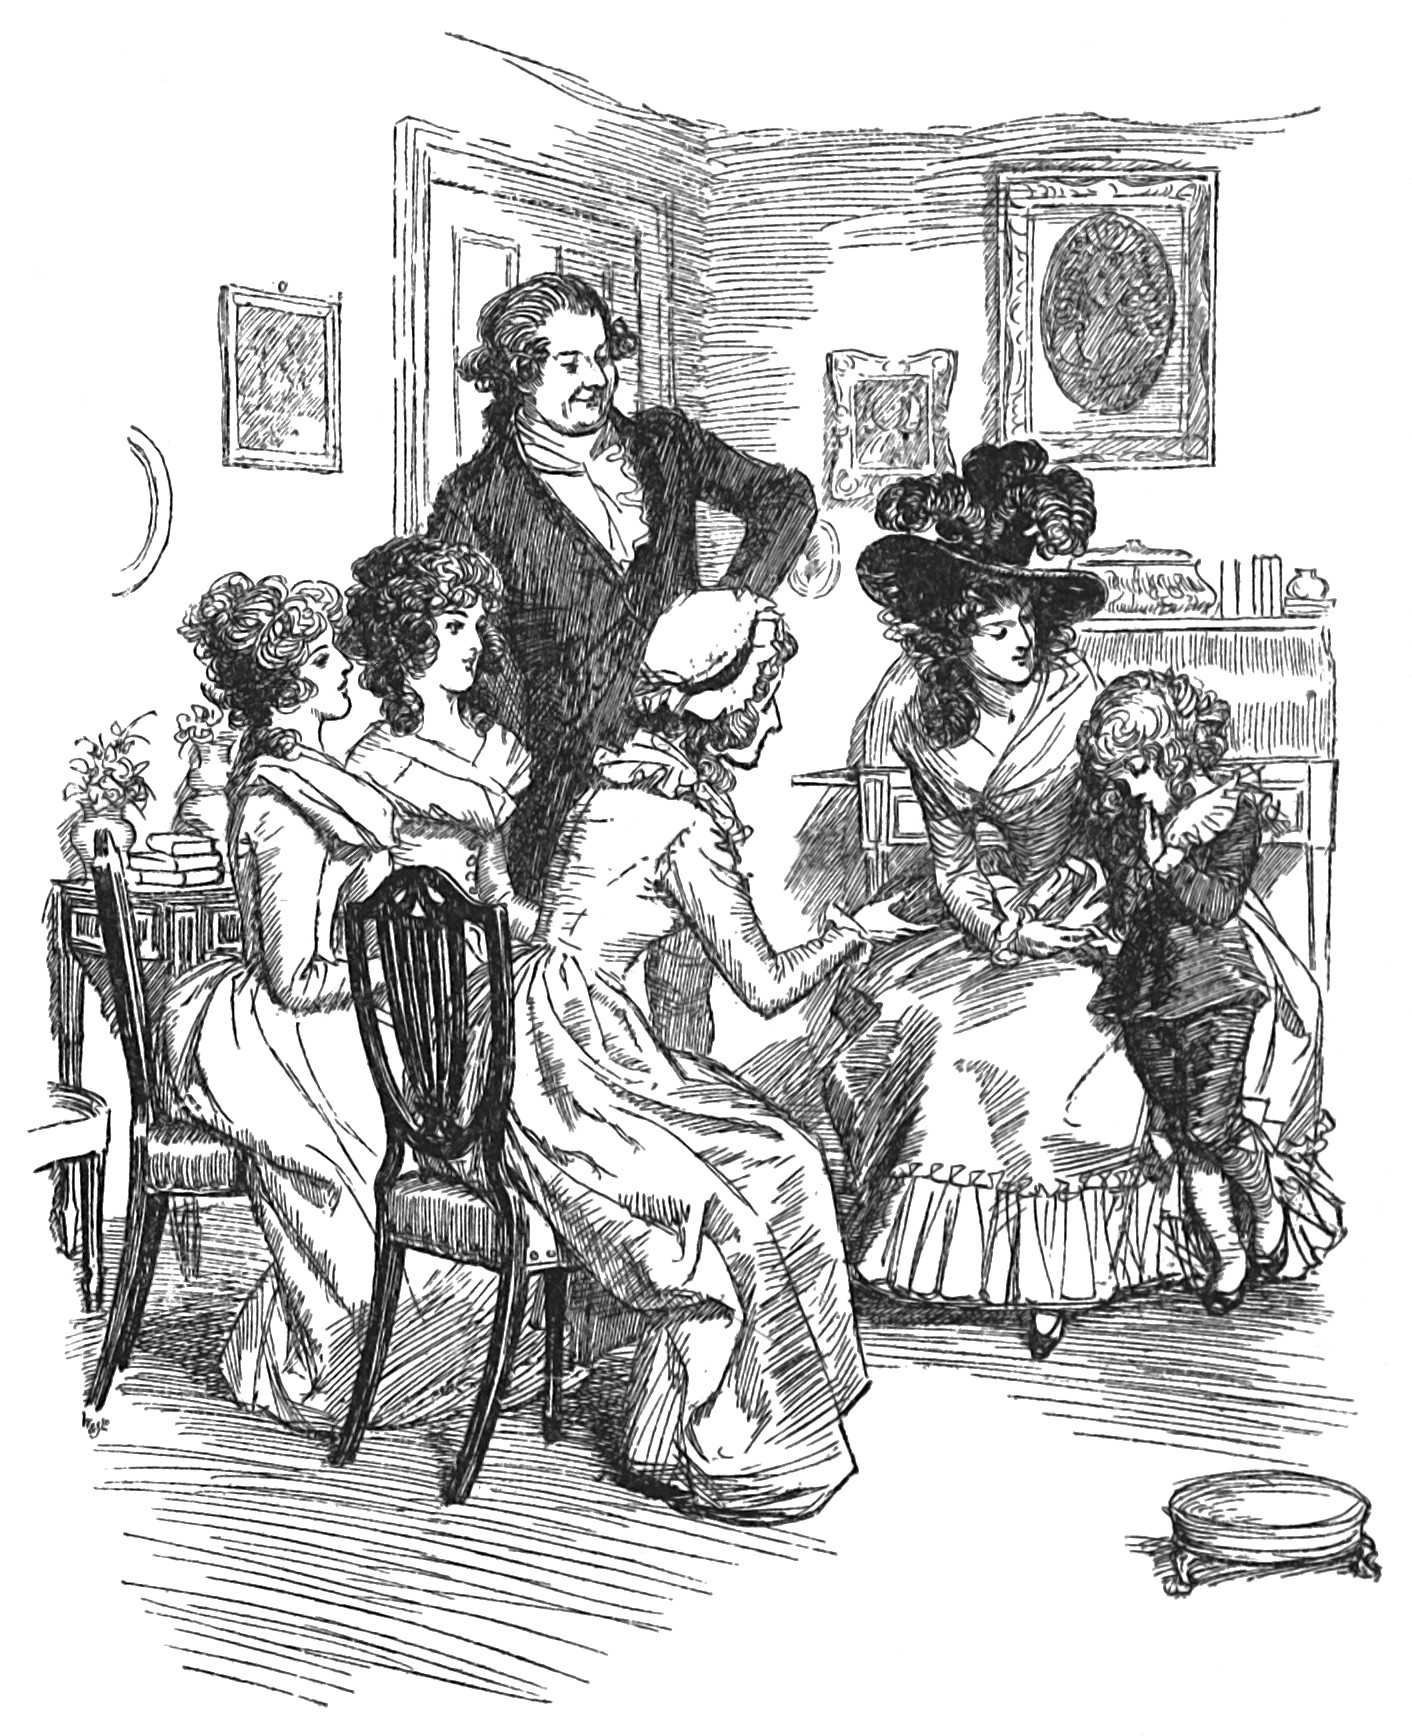
\includegraphics[width=\linewidth]{6shy}
% \caption{So shy before company}
% \end{figure}

\begin{bwbigpic}
	[1.0]
	{6shy} 
	{So shy before company} 
\end{bwbigpic}

Lady Middleton had sent a very civil message by him, denoting her intention of waiting on Mrs Dashwood as soon as she could be assured that her visit would be no inconvenience; and as this message was answered by an invitation equally polite, her ladyship was introduced to them the next day.

They were, of course, very anxious to see a person on whom so much of their comfort at Barton must depend; and the elegance of her appearance was favourable to their wishes. Lady Middleton was not more than six or seven and twenty; her face was handsome, her figure tall and striking, and her address graceful. Her manners had all the elegance which her husband's wanted. But they would have been improved by some share of his frankness and warmth; and her visit was long enough to detract something from their first admiration, by showing that, though perfectly well-bred, she was reserved, cold, and had nothing to say for herself beyond the most common-place inquiry or remark.

Conversation however was not wanted, for Sir John was very chatty, and Lady Middleton had taken the wise precaution of bringing with her their eldest child, a fine little boy about six years old, by which means there was one subject always to be recurred to by the ladies in case of extremity, for they had to enquire his name and age, admire his beauty, and ask him questions which his mother answered for him, while he hung about her and held down his head, to the great surprise of her ladyship, who wondered at his being so shy before company, as he could make noise enough at home. On every formal visit a child ought to be of the party, by way of provision for discourse. In the present case it took up ten minutes to determine whether the boy were most like his father or mother, and in what particular he resembled either, for of course every body differed, and every body was astonished at the opinion of the others.

An opportunity was soon to be given to the Dashwoods of debating on the rest of the children, as Sir John would not leave the house without securing their promise of dining at the park the next day.
\chapter{Lady~Susan Vernon to Mrs~Johnson}
  
  \begin{mail}{Churchhill.}{My dear Alicia,}
You are very good in taking notice of Frederica, and I am grateful for it as a mark of your friendship; but as I cannot have any doubt of the warmth of your affection, I am far from exacting so heavy a sacrifice. She is a stupid girl, and has nothing to recommend her. I would not, therefore, on my account, have you encumber one moment of your precious time by sending for her to Edward Street, especially as every visit is so much deducted from the grand affair of education, which I really wish to have attended to while she remains at Miss~Summers's. I want her to play and sing with some portion of taste and a good deal of assurance, as she has my hand and arm and a tolerable voice. I was so much indulged in my infant years that I was never obliged to attend to anything, and consequently am without the accomplishments which are now necessary to finish a pretty woman. Not that I am an advocate for the prevailing fashion of acquiring a perfect knowledge of all languages, arts, and sciences. It is throwing time away to be mistress of French, Italian, and German: music, singing, and drawing, \&c., will gain a woman some applause, but will not add one lover to her list—grace and manner, after all, are of the greatest importance. I do not mean, therefore, that Frederica's acquirements should be more than superficial, and I flatter myself that she will not remain long enough at school to understand anything thoroughly. I hope to see her the wife of Sir~James within a twelvemonth. You know on what I ground my hope, and it is certainly a good foundation, for school must be very humiliating to a girl of Frederica's age. And, by-the-by, you had better not invite her any more on that account, as I wish her to find her situation as unpleasant as possible. I am sure of Sir~James at any time, and could make him renew his application by a line. I shall trouble you meanwhile to prevent his forming any other attachment when he comes to town. Ask him to your house occasionally, and talk to him of Frederica, that he may not forget her. Upon the whole, I commend my own conduct in this affair extremely, and regard it as a very happy instance of circumspection and tenderness. Some mothers would have insisted on their daughter's accepting so good an offer on the first overture; but I could not reconcile it to myself to force Frederica into a marriage from which her heart revolted, and instead of adopting so harsh a measure merely propose to make it her own choice, by rendering her thoroughly uncomfortable till she does accept him—but enough of this tiresome girl. You may well wonder how I contrive to pass my time here, and for the first week it was insufferably dull. Now, however, we begin to mend, our party is enlarged by Mrs~Vernon's brother, a handsome young man, who promises me some amusement. There is something about him which rather interests me, a sort of sauciness and familiarity which I shall teach him to correct. He is lively, and seems clever, and when I have inspired him with greater respect for me than his sister's kind offices have implanted, he may be an agreeable flirt. There is exquisite pleasure in subduing an insolent spirit, in making a person predetermined to dislike acknowledge one's superiority. I have disconcerted him already by my calm reserve, and it shall be my endeavour to humble the pride of these self important De Courcys still lower, to convince Mrs~Vernon that her sisterly cautions have been bestowed in vain, and to persuade Reginald that she has scandalously belied me. This project will serve at least to amuse me, and prevent my feeling so acutely this dreadful separation from you and all whom I love.

\closeletter[Yours ever,]{S. Vernon.} 
\end{mail}
%!TeX root=../sensetop.tex
\chapter[Chapter \thechapter]{}
\lettrine[lraise=0.3]{M}{rs} Jennings was a widow with an ample jointure. She had only two daughters, both of whom she had lived to see respectably married, and she had now therefore nothing to do but to marry all the rest of the world. In the promotion of this object she was zealously active, as far as her ability reached; and missed no opportunity of projecting weddings among all the young people of her acquaintance. She was remarkably quick in the discovery of attachments, and had enjoyed the advantage of raising the blushes and the vanity of many a young lady by insinuations of her power over such a young man; and this kind of discernment enabled her soon after her arrival at Barton decisively to pronounce that Colonel Brandon was very much in love with Marianne Dashwood. She rather suspected it to be so, on the very first evening of their being together, from his listening so attentively while she sang to them; and when the visit was returned by the Middletons' dining at the cottage, the fact was ascertained by his listening to her again. It must be so. She was perfectly convinced of it. It would be an excellent match, for \textit{he} was rich, and \textit{she} was handsome. Mrs Jennings had been anxious to see Colonel Brandon well married, ever since her connection with Sir John first brought him to her knowledge; and she was always anxious to get a good husband for every pretty girl.

The immediate advantage to herself was by no means inconsiderable, for it supplied her with endless jokes against them both. At the park she laughed at the colonel, and in the cottage at Marianne. To the former her raillery was probably, as far as it regarded only himself, perfectly indifferent; but to the latter it was at first incomprehensible; and when its object was understood, she hardly knew whether most to laugh at its absurdity, or censure its impertinence, for she considered it as an unfeeling reflection on the colonel's advanced years, and on his forlorn condition as an old bachelor.

Mrs Dashwood, who could not think a man five years younger than herself, so exceedingly ancient as he appeared to the youthful fancy of her daughter, ventured to clear Mrs Jennings from the probability of wishing to throw ridicule on his age.

<But at least, Mama, you cannot deny the absurdity of the accusation, though you may not think it intentionally ill-natured. Colonel Brandon is certainly younger than Mrs Jennings, but he is old enough to be \textit{my} father; and if he were ever animated enough to be in love, must have long outlived every sensation of the kind. It is too ridiculous! When is a man to be safe from such wit, if age and infirmity will not protect him?>

<Infirmity!> said Elinor, <do you call Colonel Brandon infirm? I can easily suppose that his age may appear much greater to you than to my mother; but you can hardly deceive yourself as to his having the use of his limbs!>

<Did not you hear him complain of the rheumatism? and is not that the commonest infirmity of declining life?>

<My dearest child,> said her mother, laughing, <at this rate you must be in continual terror of \textit{my} decay; and it must seem to you a miracle that my life has been extended to the advanced age of forty.>

<Mama, you are not doing me justice. I know very well that Colonel Brandon is not old enough to make his friends yet apprehensive of losing him in the course of nature. He may live twenty years longer. But thirty-five has nothing to do with matrimony.>

<Perhaps,> said Elinor, <thirty-five and seventeen had better not have any thing to do with matrimony together. But if there should by any chance happen to be a woman who is single at seven and twenty, I should not think Colonel Brandon's being thirty-five any objection to his marrying \textit{her}.>

<A woman of seven and twenty,> said Marianne, after pausing a moment, <can never hope to feel or inspire affection again, and if her home be uncomfortable, or her fortune small, I can suppose that she might bring herself to submit to the offices of a nurse, for the sake of the provision and security of a wife. In his marrying such a woman therefore there would be nothing unsuitable. It would be a compact of convenience, and the world would be satisfied. In my eyes it would be no marriage at all, but that would be nothing. To me it would seem only a commercial exchange, in which each wished to be benefited at the expense of the other.>

<It would be impossible, I know,> replied Elinor, <to convince you that a woman of seven and twenty could feel for a man of thirty-five anything near enough to love, to make him a desirable companion to her. But I must object to your dooming Colonel Brandon and his wife to the constant confinement of a sick chamber, merely because he chanced to complain yesterday (a very cold damp day) of a slight rheumatic feel in one of his shoulders.>

<But he talked of flannel waistcoats,> said Marianne; <and with me a flannel waistcoat is invariably connected with aches, cramps, rheumatisms, and every species of ailment that can afflict the old and the feeble.>

<Had he been only in a violent fever, you would not have despised him half so much. Confess, Marianne, is not there something interesting to you in the flushed cheek, hollow eye, and quick pulse of a fever?>

Soon after this, upon Elinor's leaving the room, <Mama,> said Marianne, <I have an alarm on the subject of illness which I cannot conceal from you. I am sure Edward Ferrars is not well. We have now been here almost a fortnight, and yet he does not come. Nothing but real indisposition could occasion this extraordinary delay. What else can detain him at Norland?>

<Had you any idea of his coming so soon?> said Mrs Dashwood. <\textit{I} had none. On the contrary, if I have felt any anxiety at all on the subject, it has been in recollecting that he sometimes showed a want of pleasure and readiness in accepting my invitation, when I talked of his coming to Barton. Does Elinor expect him already?>

<I have never mentioned it to her, but of course she must.>

<I rather think you are mistaken, for when I was talking to her yesterday of getting a new grate for the spare bedchamber, she observed that there was no immediate hurry for it, as it was not likely that the room would be wanted for some time.>

<How strange this is! what can be the meaning of it! But the whole of their behaviour to each other has been unaccountable! How cold, how composed were their last adieus! How languid their conversation the last evening of their being together! In Edward's farewell there was no distinction between Elinor and me: it was the good wishes of an affectionate brother to both. Twice did I leave them purposely together in the course of the last morning, and each time did he most unaccountably follow me out of the room. And Elinor, in quitting Norland and Edward, cried not as I did. Even now her self-command is invariable. When is she dejected or melancholy? When does she try to avoid society, or appear restless and dissatisfied in it?>
%!TeX root=../pridetop.tex

\chapter[Chapter \thechapter]{}
	
	\begin{figure}[t!]
\centering
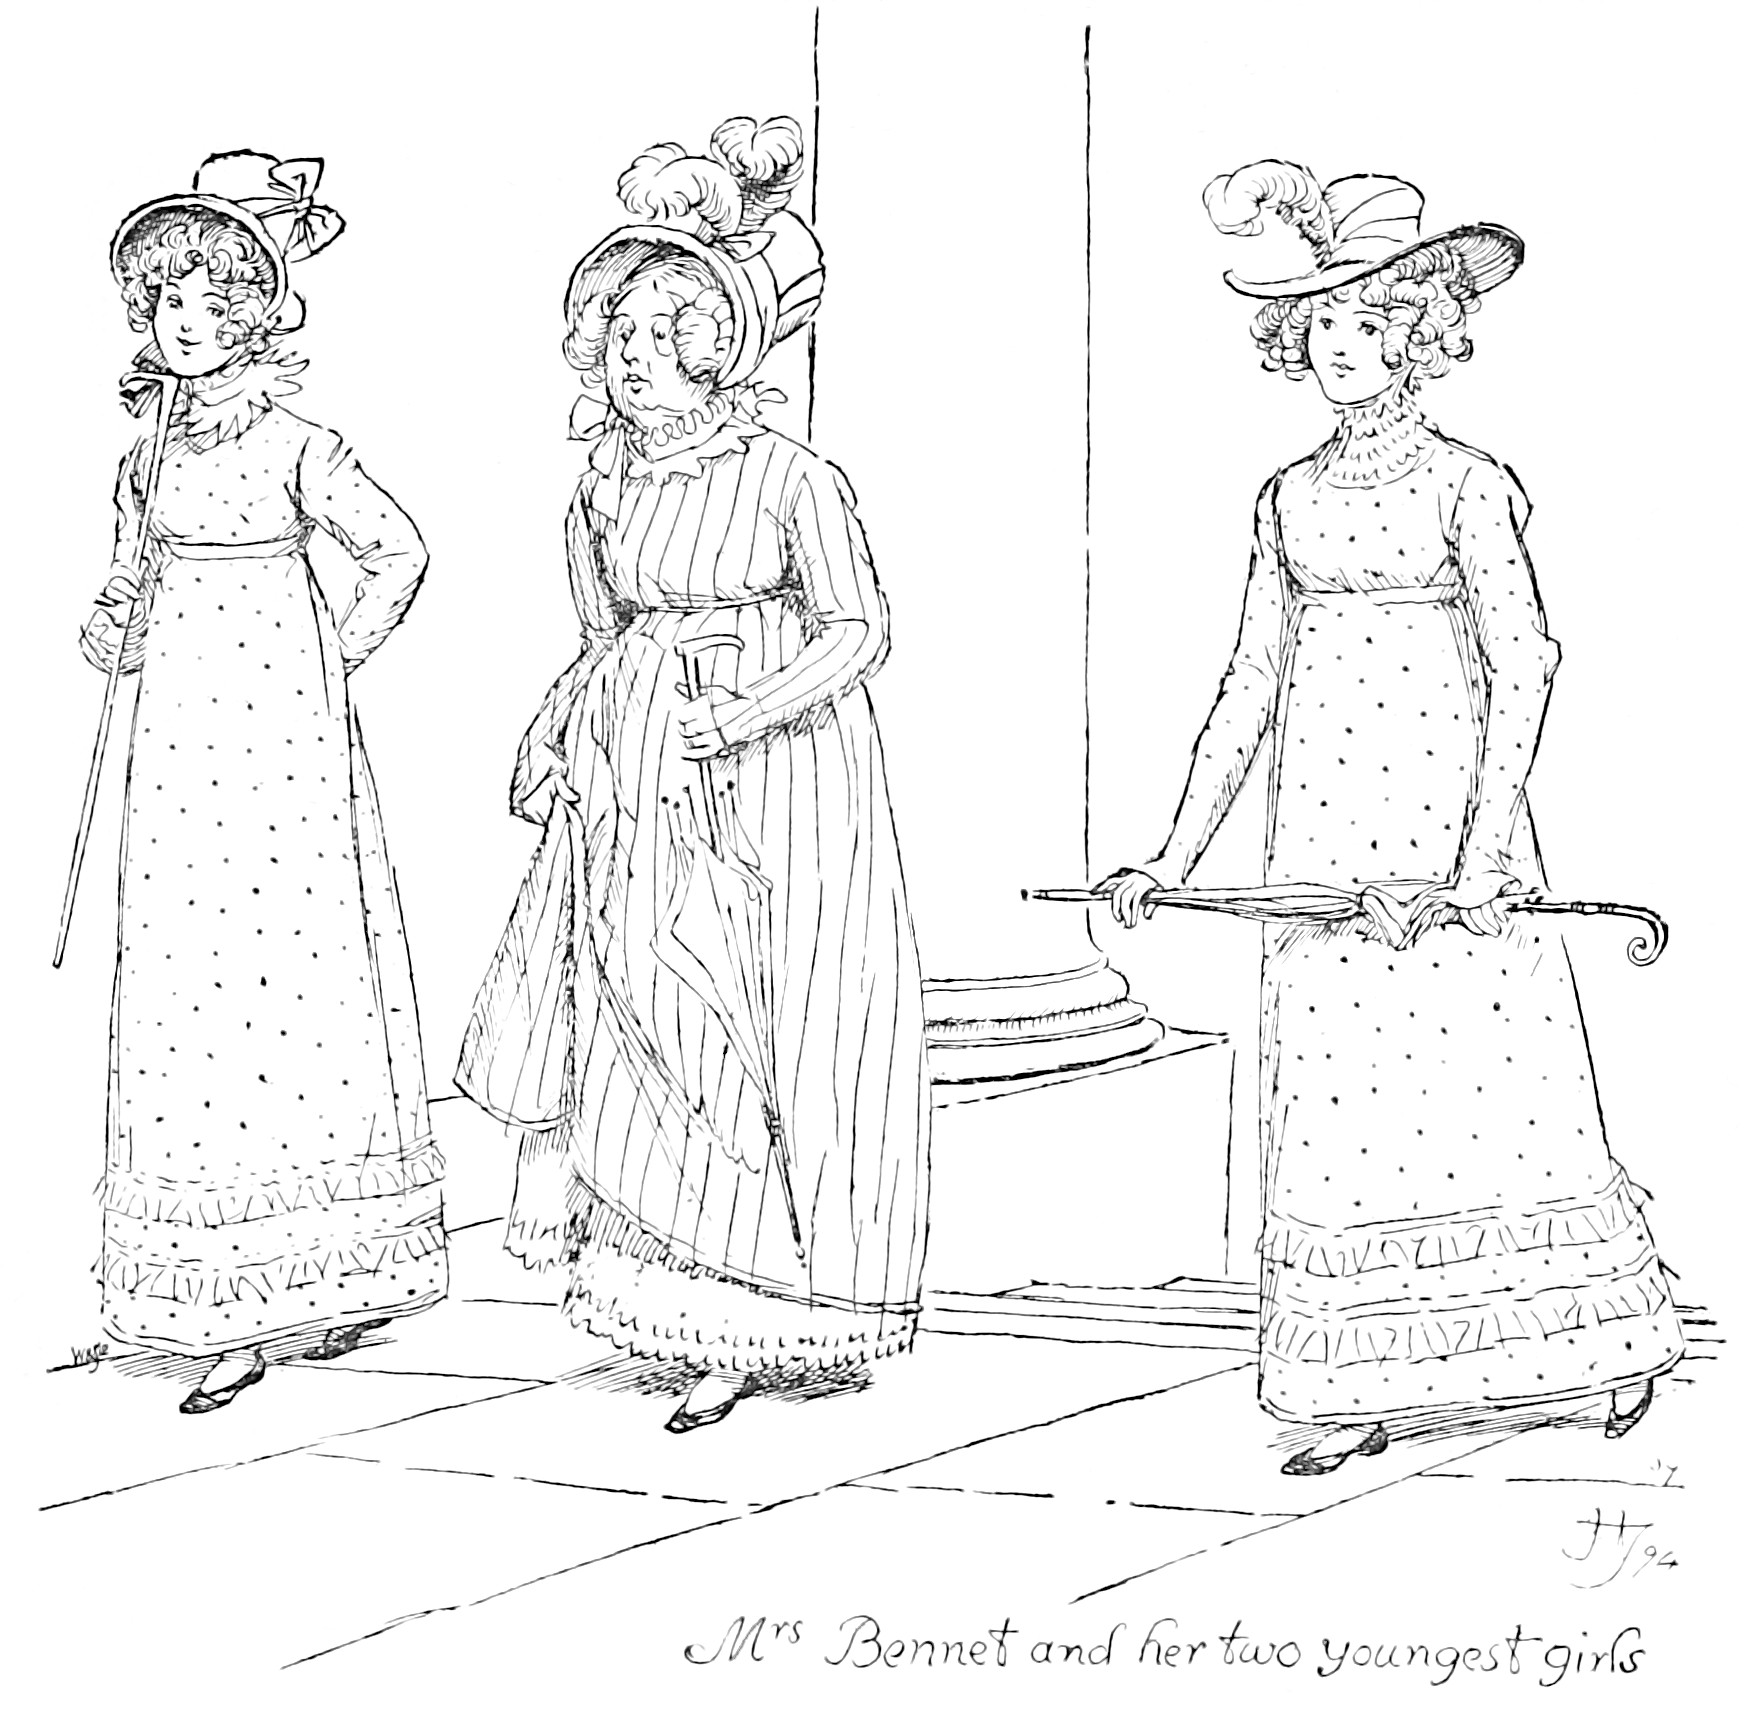
\includegraphics[width=.8\linewidth]{9bennetgirls}
\captionlistentry{Mrs Bennet and her two youngest girls}
\end{figure}

	\lettrine[lines=6,image=true]{initials/chap9e}{lizabeth}  passed the chief of the night in her sister's room, and in the morning had the pleasure of being able to send a tolerable answer to the inquiries which she very early received from Mr Bingley by a housemaid, and some time afterwards from the two elegant ladies who waited on his sisters. In spite of this amendment, however, she requested to have a note sent to Longbourn, desiring her mother to visit Jane, and form her own judgment of her situation. The note was immediately despatched, and its contents as quickly complied with. Mrs Bennet, accompanied by her two youngest girls, reached Netherfield soon after the family breakfast.



Had she found Jane in any apparent danger, Mrs Bennet would have been very miserable; but being satisfied on seeing her that her illness was not alarming, she had no wish of her recovering immediately, as her restoration to health would probably remove her from Netherfield. She would not listen, therefore, to her daughter's proposal of being carried home; neither did the apothecary, who arrived about the same time, think it at all advisable. After sitting a little while with Jane, on Miss Bingley's appearance and invitation, the mother and three daughters all attended her into the breakfast parlour. Bingley met them with hopes that Mrs Bennet had not found Miss Bennet worse than she expected.

»Indeed I have, sir,« was her answer. »She is a great deal too ill to be moved. Mr Jones says we must not think of moving her. We must trespass a little longer on your kindness.«

»Removed!« cried Bingley. »It must not be thought of. My sister, I am sure, will not hear of her removal.«

»You may depend upon it, madam,« said Miss Bingley, with cold civility, »that Miss Bennet shall receive every possible attention while she remains with us.«

Mrs Bennet was profuse in her acknowledgments.

»I am sure,« she added, »if it was not for such good friends, I do not know what would become of her, for she is very ill indeed, and suffers a vast deal, though with the greatest patience in the world, which is always the way with her, for she has, without exception, the sweetest temper I ever met with. I often tell my other girls they are nothing to \textit{her}. You have a sweet room here, Mr Bingley, and a charming prospect over that gravel walk. I do not know a place in the country that is equal to Netherfield. You will not think of quitting it in a hurry, I hope, though you have but a short lease.«

»Whatever I do is done in a hurry,« replied he; »and therefore if I should resolve to quit Netherfield, I should probably be off in five minutes. At present, however, I consider myself as quite fixed here.«

»That is exactly what I should have supposed of you,« said Elizabeth.

»You begin to comprehend me, do you?« cried he, turning towards her.

»Oh yes—I understand you perfectly.«

»I wish I might take this for a compliment; but to be so easily seen through, I am afraid, is pitiful.«

»That is as it happens. It does not necessarily follow that a deep, intricate character is more or less estimable than such a one as yours.«

»Lizzy,« cried her mother, »remember where you are, and do not run on in the wild manner that you are suffered to do at home.«

»I did not know before,« continued Bingley, immediately, »that you were a studier of character. It must be an amusing study.«

»Yes; but intricate characters are the \textit{most} amusing. They have at least that advantage.«

»The country,« said Darcy, »can in general supply but few subjects for such a study. In a country neighbourhood you move in a very confined and unvarying society.«

»But people themselves alter so much, that there is something new to be observed in them for ever.«

»Yes, indeed,« cried Mrs Bennet, offended by his manner of mentioning a country neighbourhood. »I assure you there is quite as much of \textit{that} going on in the country as in town.«

Everybody was surprised; and Darcy, after looking at her for a moment, turned silently away. Mrs Bennet, who fancied she had gained a complete victory over him, continued her triumph,—

»I cannot see that London has any great advantage over the country, for my part, except the shops and public places. The country is a vast deal pleasanter, is not it, Mr Bingley?«

»When I am in the country,« he replied, »I never wish to leave it; and when I am in town, it is pretty much the same. They have each their advantages, and I can be equally happy in either.«

»Ay, that is because you have the right disposition. But that gentleman,« looking at Darcy, »seemed to think the country was nothing at all.«

»Indeed, mamma, you are mistaken,« said Elizabeth, blushing for her mother. »You quite mistook Mr Darcy. He only meant that there was not such a variety of people to be met with in the country as in town, which you must acknowledge to be true.«

»Certainly, my dear, nobody said there were; but as to not meeting with many people in this neighbourhood, I believe there are few neighbourhoods larger. I know we dine with four-and-twenty families.«

Nothing but concern for Elizabeth could enable Bingley to keep his countenance. His sister was less delicate, and directed her eye towards Mr Darcy with a very expressive smile. Elizabeth, for the sake of saying something that might turn her mother's thoughts, now asked her if Charlotte Lucas had been at Longbourn since \textit{her} coming away.

»Yes, she called yesterday with her father. What an agreeable man Sir William is, Mr Bingley—is not he? so much the man of fashion! so genteel and so easy! He has always something to say to everybody. \textit{That} is my idea of good breeding; and those persons who fancy themselves very important and never open their mouths quite mistake the matter.«

»Did Charlotte dine with you?«

»No, she would go home. I fancy she was wanted about the mince-pies. For my part, Mr Bingley, \textit{I} always keep servants that can do their own work; \textit{my} daughters are brought up differently. But everybody is to judge for themselves, and the Lucases are a very good sort of girls, I assure you. It is a pity they are not handsome! Not that \textit{I} think Charlotte so \textit{very} plain; but then she is our particular friend.«

»She seems a very pleasant young woman,« said Bingley.

»Oh dear, yes; but you must own she is very plain. Lady Lucas herself has often said so, and envied me Jane's beauty. I do not like to boast of my own child; but to be sure, Jane—one does not often see anybody better looking. It is what everybody says. I do not trust my own partiality. When she was only fifteen there was a gentleman at my brother Gardiner's in town so much in love with her, that my sister-in-law was sure he would make her an offer before we came away. But, however, he did not. Perhaps he thought her too young. However, he wrote some verses on her, and very pretty they were.«

»And so ended his affection,« said Elizabeth, impatiently. »There has been many a one, I fancy, overcome in the same way. I wonder who first discovered the efficacy of poetry in driving away love!«

»I have been used to consider poetry as the \textit{food} of love,« said Darcy.

»Of a fine, stout, healthy love it may. Everything nourishes what is strong already. But if it be only a slight, thin sort of inclination, I am convinced that one good sonnet will starve it entirely away.«

Darcy only smiled; and the general pause which ensued made Elizabeth tremble lest her mother should be exposing herself again. She longed to speak, but could think of nothing to say; and after a short silence Mrs Bennet began repeating her thanks to Mr Bingley for his kindness to Jane, with an apology for troubling him also with Lizzy. Mr Bingley was unaffectedly civil in his answer, and forced his younger sister to be civil also, and say what the occasion required. She performed her part, indeed, without much graciousness, but Mrs Bennet was satisfied, and soon afterwards ordered her carriage. Upon this signal, the youngest of her daughters put herself forward. The two girls had been whispering to each other during the whole visit; and the result of it was, that the youngest should tax Mr Bingley with having promised on his first coming into the country to give a ball at Netherfield.

Lydia was a stout, well-grown girl of fifteen, with a fine complexion and good-humoured countenance; a favourite with her mother, whose affection had brought her into public at an early age. She had high animal spirits, and a sort of natural \newline self-consequence, which the attentions of the officers, to whom her uncle's good dinners and her own easy manners recommended her, had increased into assurance. She was very equal, therefore, to address Mr Bingley on the subject of the ball, and abruptly reminded him of his promise; adding, that it would be the most shameful thing in the world if he did not keep it. His answer to this sudden attack was delightful to her mother's ear.

»I am perfectly ready, I assure you, to keep my engagement; and, when your sister is recovered, you shall, if you please, name the very day of the ball. But you would not wish to be dancing while she is ill?«

Lydia declared herself satisfied. »Oh yes—it would be much better to wait till Jane was well; and by that time, most likely, Captain Carter would be at Meryton again. And when you have given \textit{your} ball,« she added, »I shall insist on their giving one also. I shall tell Colonel Forster it will be quite a shame if he does not.«

Mrs Bennet and her daughters then departed, and Elizabeth returned instantly to Jane, leaving her own and her relations' behaviour to the remarks of the two ladies and Mr Darcy; the latter of whom, however, could not be prevailed on to join in their censure of \textit{her}, in spite of all Miss Bingley's witticisms on \textit{fine eyes}.
%!TeX root=../emmatop.tex
\chapter[Chapter \thechapter]{}
\lettrine[lraise=0.3]{T}{hough} now the middle of December, there had yet been no weather to prevent the young ladies from tolerably regular exercise; and on the morrow, Emma had a charitable visit to pay to a poor sick family, who lived a little way out of Highbury.

Their road to this detached cottage was down Vicarage Lane, a lane leading at right angles from the broad, though irregular, main street of the place; and, as may be inferred, containing the blessed abode of Mr Elton. A few inferior dwellings were first to be passed, and then, about a quarter of a mile down the lane rose the Vicarage, an old and not very good house, almost as close to the road as it could be. It had no advantage of situation; but had been very much smartened up by the present proprietor; and, such as it was, there could be no possibility of the two friends passing it without a slackened pace and observing eyes.—Emma's remark was—

<There it is. There go you and your riddle-book one of these days.>—Harriet's was—

<Oh, what a sweet house!—How very beautiful!—There are the yellow curtains that Miss Nash admires so much.>

<I do not often walk this way \textit{now},> said Emma, as they proceeded, <but \textit{then} there will be an inducement, and I shall gradually get intimately acquainted with all the hedges, gates, pools and pollards of this part of Highbury.>

Harriet, she found, had never in her life been inside the Vicarage, and her curiosity to see it was so extreme, that, considering exteriors and probabilities, Emma could only class it, as a proof of love, with Mr Elton's seeing ready wit in her.

<I wish we could contrive it,> said she; <but I cannot think of any tolerable pretence for going in;—no servant that I want to inquire about of his housekeeper—no message from my father.>

She pondered, but could think of nothing. After a mutual silence of some minutes, Harriet thus began again—

<I do so wonder, Miss Woodhouse, that you should not be married, or going to be married! so charming as you are!>—

Emma laughed, and replied,

<My being charming, Harriet, is not quite enough to induce me to marry; I must find other people charming—one other person at least. And I am not only, not going to be married, at present, but have very little intention of ever marrying at all.>

<Ah!—so you say; but I cannot believe it.>

<I must see somebody very superior to any one I have seen yet, to be tempted; Mr Elton, you know, (recollecting herself,) is out of the question: and I do \textit{not} wish to see any such person. I would rather not be tempted. I cannot really change for the better. If I were to marry, I must expect to repent it.>

<Dear me!—it is so odd to hear a woman talk so!>—

<I have none of the usual inducements of women to marry. Were I to fall in love, indeed, it would be a different thing! but I never have been in love; it is not my way, or my nature; and I do not think I ever shall. And, without love, I am sure I should be a fool to change such a situation as mine. Fortune I do not want; employment I do not want; consequence I do not want: I believe few married women are half as much mistress of their husband's house as I am of Hartfield; and never, never could I expect to be so truly beloved and important; so always first and always right in any man's eyes as I am in my father's.>

<But then, to be an old maid at last, like Miss Bates!>

<That is as formidable an image as you could present, Harriet; and if I thought I should ever be like Miss Bates! so silly—so satisfied—so smiling—so prosing—so undistinguishing and unfastidious—and so apt to tell every thing relative to every body about me, I would marry to-morrow. But between \textit{us}, I am convinced there never can be any likeness, except in being unmarried.>

<But still, you will be an old maid! and that's so dreadful!>

<Never mind, Harriet, I shall not be a poor old maid; and it is poverty only which makes celibacy contemptible to a generous public! A single woman, with a very narrow income, must be a ridiculous, disagreeable old maid! the proper sport of boys and girls, but a single woman, of good fortune, is always respectable, and may be as sensible and pleasant as any body else. And the distinction is not quite so much against the candour and common sense of the world as appears at first; for a very narrow income has a tendency to contract the mind, and sour the temper. Those who can barely live, and who live perforce in a very small, and generally very inferior, society, may well be illiberal and cross. This does not apply, however, to Miss Bates; she is only too good natured and too silly to suit me; but, in general, she is very much to the taste of every body, though single and though poor. Poverty certainly has not contracted her mind: I really believe, if she had only a shilling in the world, she would be very likely to give away sixpence of it; and nobody is afraid of her: that is a great charm.>

<Dear me! but what shall you do? how shall you employ yourself when you grow old?>

<If I know myself, Harriet, mine is an active, busy mind, with a great many independent resources; and I do not perceive why I should be more in want of employment at forty or fifty than one-and-twenty. Woman's usual occupations of hand and mind will be as open to me then as they are now; or with no important variation. If I draw less, I shall read more; if I give up music, I shall take to carpet-work. And as for objects of interest, objects for the affections, which is in truth the great point of inferiority, the want of which is really the great evil to be avoided in \textit{not} marrying, I shall be very well off, with all the children of a sister I love so much, to care about. There will be enough of them, in all probability, to supply every sort of sensation that declining life can need. There will be enough for every hope and every fear; and though my attachment to none can equal that of a parent, it suits my ideas of comfort better than what is warmer and blinder. My nephews and nieces!—I shall often have a niece with me.>

<Do you know Miss Bates's niece? That is, I know you must have seen her a hundred times—but are you acquainted?>

<Oh! yes; we are always forced to be acquainted whenever she comes to Highbury. By the bye, \textit{that} is almost enough to put one out of conceit with a niece. Heaven forbid! at least, that I should ever bore people half so much about all the Knightleys together, as she does about Jane Fairfax. One is sick of the very name of Jane Fairfax. Every letter from her is read forty times over; her compliments to all friends go round and round again; and if she does but send her aunt the pattern of a stomacher, or knit a pair of garters for her grandmother, one hears of nothing else for a month. I wish Jane Fairfax very well; but she tires me to death.>

They were now approaching the cottage, and all idle topics were superseded. Emma was very compassionate; and the distresses of the poor were as sure of relief from her personal attention and kindness, her counsel and her patience, as from her purse. She understood their ways, could allow for their ignorance and their temptations, had no romantic expectations of extraordinary virtue from those for whom education had done so little; entered into their troubles with ready sympathy, and always gave her assistance with as much intelligence as good-will. In the present instance, it was sickness and poverty together which she came to visit; and after remaining there as long as she could give comfort or advice, she quitted the cottage with such an impression of the scene as made her say to Harriet, as they walked away,

<These are the sights, Harriet, to do one good. How trifling they make every thing else appear!—I feel now as if I could think of nothing but these poor creatures all the rest of the day; and yet, who can say how soon it may all vanish from my mind?>

<Very true,> said Harriet. <Poor creatures! one can think of nothing else.>

<And really, I do not think the impression will soon be over,> said Emma, as she crossed the low hedge, and tottering footstep which ended the narrow, slippery path through the cottage garden, and brought them into the lane again. <I do not think it will,> stopping to look once more at all the outward wretchedness of the place, and recall the still greater within.

<Oh! dear, no,> said her companion.

They walked on. The lane made a slight bend; and when that bend was passed, Mr Elton was immediately in sight; and so near as to give Emma time only to say farther,

<Ah! Harriet, here comes a very sudden trial of our stability in good thoughts. Well, (smiling,) I hope it may be allowed that if compassion has produced exertion and relief to the sufferers, it has done all that is truly important. If we feel for the wretched, enough to do all we can for them, the rest is empty sympathy, only distressing to ourselves.>

Harriet could just answer, <Oh! dear, yes,> before the gentleman joined them. The wants and sufferings of the poor family, however, were the first subject on meeting. He had been going to call on them. His visit he would now defer; but they had a very interesting parley about what could be done and should be done. Mr Elton then turned back to accompany them.

<To fall in with each other on such an errand as this,> thought Emma; <to meet in a charitable scheme; this will bring a great increase of love on each side. I should not wonder if it were to bring on the declaration. It must, if I were not here. I wish I were anywhere else.>

Anxious to separate herself from them as far as she could, she soon afterwards took possession of a narrow footpath, a little raised on one side of the lane, leaving them together in the main road. But she had not been there two minutes when she found that Harriet's habits of dependence and imitation were bringing her up too, and that, in short, they would both be soon after her. This would not do; she immediately stopped, under pretence of having some alteration to make in the lacing of her half-boot, and stooping down in complete occupation of the footpath, begged them to have the goodness to walk on, and she would follow in half a minute. They did as they were desired; and by the time she judged it reasonable to have done with her boot, she had the comfort of farther delay in her power, being overtaken by a child from the cottage, setting out, according to orders, with her pitcher, to fetch broth from Hartfield. To walk by the side of this child, and talk to and question her, was the most natural thing in the world, or would have been the most natural, had she been acting just then without design; and by this means the others were still able to keep ahead, without any obligation of waiting for her. She gained on them, however, involuntarily: the child's pace was quick, and theirs rather slow; and she was the more concerned at it, from their being evidently in a conversation which interested them. Mr Elton was speaking with animation, Harriet listening with a very pleased attention; and Emma, having sent the child on, was beginning to think how she might draw back a little more, when they both looked around, and she was obliged to join them.

Mr Elton was still talking, still engaged in some interesting detail; and Emma experienced some disappointment when she found that he was only giving his fair companion an account of the yesterday's party at his friend Cole's, and that she was come in herself for the Stilton cheese, the north Wiltshire, the butter, the celery, the beet-root, and all the dessert.

<This would soon have led to something better, of course,> was her consoling reflection; <any thing interests between those who love; and any thing will serve as introduction to what is near the heart. If I could but have kept longer away!>

They now walked on together quietly, till within view of the vicarage pales, when a sudden resolution, of at least getting Harriet into the house, made her again find something very much amiss about her boot, and fall behind to arrange it once more. She then broke the lace off short, and dexterously throwing it into a ditch, was presently obliged to entreat them to stop, and acknowledged her inability to put herself to rights so as to be able to walk home in tolerable comfort.

<Part of my lace is gone,> said she, <and I do not know how I am to contrive. I really am a most troublesome companion to you both, but I hope I am not often so ill-equipped. Mr Elton, I must beg leave to stop at your house, and ask your housekeeper for a bit of ribband or string, or any thing just to keep my boot on.>

Mr Elton looked all happiness at this proposition; and nothing could exceed his alertness and attention in conducting them into his house and endeavouring to make every thing appear to advantage. The room they were taken into was the one he chiefly occupied, and looking forwards; behind it was another with which it immediately communicated; the door between them was open, and Emma passed into it with the housekeeper to receive her assistance in the most comfortable manner. She was obliged to leave the door ajar as she found it; but she fully intended that Mr Elton should close it. It was not closed, however, it still remained ajar; but by engaging the housekeeper in incessant conversation, she hoped to make it practicable for him to chuse his own subject in the adjoining room. For ten minutes she could hear nothing but herself. It could be protracted no longer. She was then obliged to be finished, and make her appearance.

The lovers were standing together at one of the windows. It had a most favourable aspect; and, for half a minute, Emma felt the glory of having schemed successfully. But it would not do; he had not come to the point. He had been most agreeable, most delightful; he had told Harriet that he had seen them go by, and had purposely followed them; other little gallantries and allusions had been dropt, but nothing serious.

<Cautious, very cautious,> thought Emma; <he advances inch by inch, and will hazard nothing till he believes himself secure.>

Still, however, though every thing had not been accomplished by her ingenious device, she could not but flatter herself that it had been the occasion of much present enjoyment to both, and must be leading them forward to the great event.
%!TeX root=../persuasiontop.tex
\chapter[Chapter \thechapter]{}

\begin{figure}[t!]
\centering
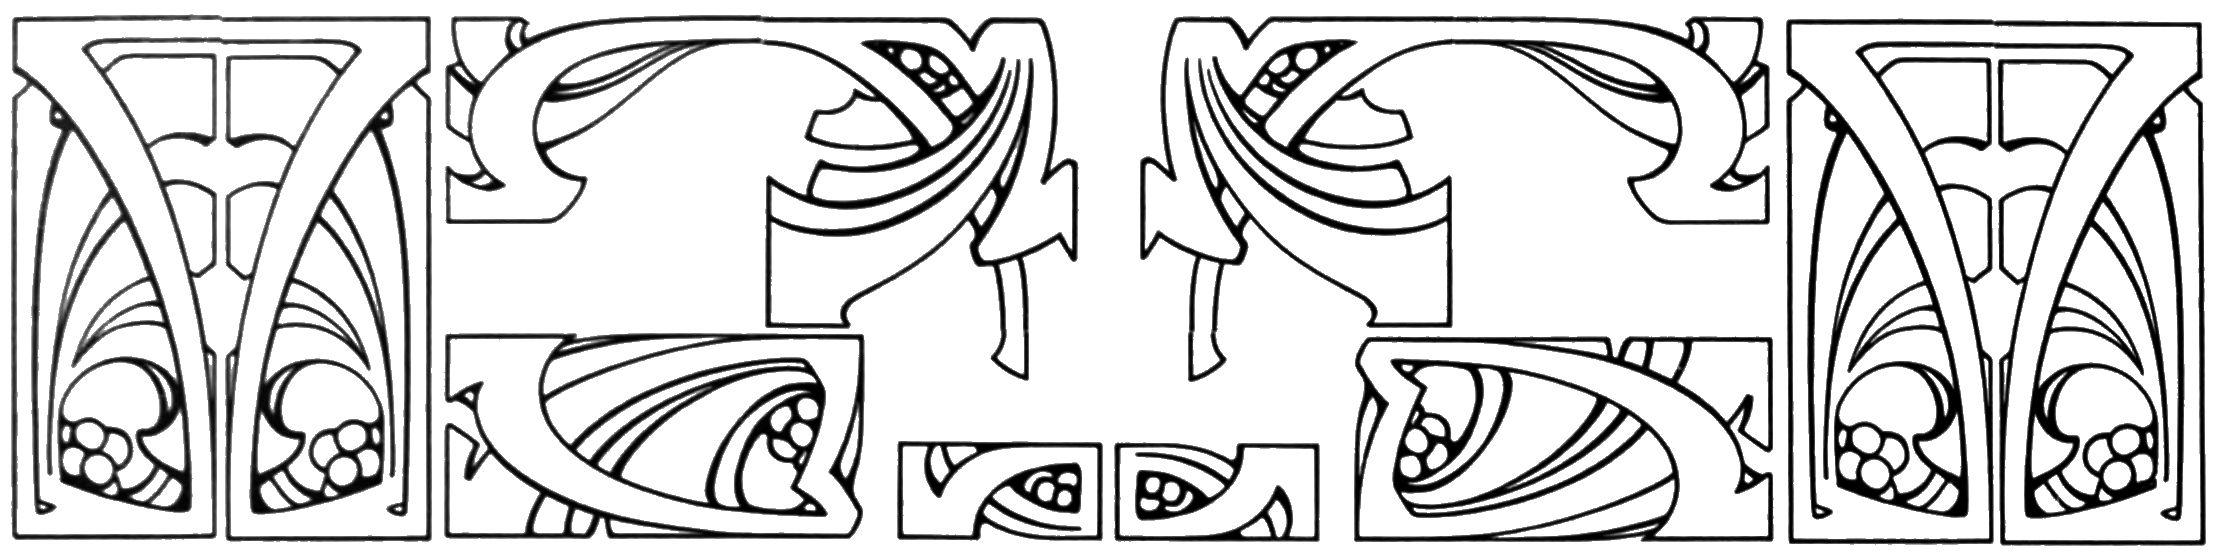
\includegraphics[width=\linewidth]{nouveau11}
\end{figure}

\lettrine[lines=4,lraise=0.3]{T}{he} time now approached for Lady Russell's return: the day was even fixed; and Anne, being engaged to join her as soon as she was resettled, was looking forward to an early removal to Kellynch, and beginning to think how her own comfort was likely to be affected by it.

It would place her in the same village with Captain Wentworth, within half a mile of him; they would have to frequent the same church, and there must be intercourse between the two families. This was against her; but on the other hand, he spent so much of his time at Uppercross, that in removing thence she might be considered rather as leaving him behind, than as going towards him; and, upon the whole, she believed she must, on this interesting question, be the gainer, almost as certainly as in her change of domestic society, in leaving poor Mary for Lady Russell.

She wished it might be possible for her to avoid ever seeing Captain Wentworth at the Hall: those rooms had witnessed former meetings which would be brought too painfully before her; but she was yet more anxious for the possibility of Lady Russell and Captain Wentworth never meeting anywhere. They did not like each other, and no renewal of acquaintance now could do any good; and were Lady Russell to see them together, she might think that he had too much self-possession, and she too little.

These points formed her chief solicitude in anticipating her removal from Uppercross, where she felt she had been stationed quite long enough. Her usefulness to little Charles would always give some sweetness to the memory of her two months' visit there, but he was gaining strength apace, and she had nothing else to stay for.

The conclusion of her visit, however, was diversified in a way which she had not at all imagined. Captain Wentworth, after being unseen and unheard of at Uppercross for two whole days, appeared again among them to justify himself by a relation of what had kept him away.

A letter from his friend, Captain Harville, having found him out at last, had brought intelligence of Captain Harville's being settled with his family at Lyme for the winter; of their being therefore, quite unknowingly, within twenty miles of each other. Captain Harville had never been in good health since a severe wound which he received two years before, and Captain Wentworth's anxiety to see him had determined him to go immediately to Lyme. He had been there for four-and-twenty hours. His acquittal was complete, his friendship warmly honoured, a lively interest excited for his friend, and his description of the fine country about Lyme so feelingly attended to by the party, that an earnest desire to see Lyme themselves, and a project for going thither was the consequence.

The young people were all wild to see Lyme. Captain Wentworth talked of going there again himself, it was only seventeen miles from Uppercross; though November, the weather was by no means bad; and, in short, Louisa, who was the most eager of the eager, having formed the resolution to go, and besides the pleasure of doing as she liked, being now armed with the idea of merit in maintaining her own way, bore down all the wishes of her father and mother for putting it off till summer; and to Lyme they were to go—Charles, Mary, Anne, Henrietta, Louisa, and Captain Wentworth.

The first heedless scheme had been to go in the morning and return at night; but to this Mr Musgrove, for the sake of his horses, would not consent; and when it came to be rationally considered, a day in the middle of November would not leave much time for seeing a new place, after deducting seven hours, as the nature of the country required, for going and returning. They were, consequently, to stay the night there, and not to be expected back till the next day's dinner. This was felt to be a considerable amendment; and though they all met at the Great House at rather an early breakfast hour, and set off very punctually, it was so much past noon before the two carriages, Mr Musgrove's coach containing the four ladies, and Charles's curricle, in which he drove Captain Wentworth, were descending the long hill into Lyme, and entering upon the still steeper street of the town itself, that it was very evident they would not have more than time for looking about them, before the light and warmth of the day were gone.

After securing accommodations, and ordering a dinner at one of the inns, the next thing to be done was unquestionably to walk directly down to the sea. They were come too late in the year for any amusement or variety which Lyme, as a public place, might offer. The rooms were shut up, the lodgers almost all gone, scarcely any family but of the residents left; and, as there is nothing to admire in the buildings themselves, the remarkable situation of the town, the principal street almost hurrying into the water, the walk to the Cobb, skirting round the pleasant little bay, which, in the season, is animated with bathing machines and company; the Cobb itself, its old wonders and new improvements, with the very beautiful line of cliffs stretching out to the east of the town, are what the stranger's eye will seek; and a very strange stranger it must be, who does not see charms in the immediate environs of Lyme, to make him wish to know it better. The scenes in its neighbourhood, Charmouth, with its high grounds and extensive sweeps of country, and still more, its sweet, retired bay, backed by dark cliffs, where fragments of low rock among the sands, make it the happiest spot for watching the flow of the tide, for sitting in unwearied contemplation; the woody varieties of the cheerful village of Up Lyme; and, above all, Pinny, with its green chasms between romantic rocks, where the scattered forest trees and orchards of luxuriant growth, declare that many a generation must have passed away since the first partial falling of the cliff prepared the ground for such a state, where a scene so wonderful and so lovely is exhibited, as may more than equal any of the resembling scenes of the far-famed Isle of Wight: these places must be visited, and visited again, to make the worth of Lyme understood.

The party from Uppercross passing down by the now deserted and melancholy looking rooms, and still descending, soon found themselves on the sea-shore; and lingering only, as all must linger and gaze on a first return to the sea, who ever deserved to look on it at all, proceeded towards the Cobb, equally their object in itself and on Captain Wentworth's account: for in a small house, near the foot of an old pier of unknown date, were the Harvilles settled. Captain Wentworth turned in to call on his friend; the others walked on, and he was to join them on the Cobb.

They were by no means tired of wondering and admiring; and not even Louisa seemed to feel that they had parted with Captain Wentworth long, when they saw him coming after them, with three companions, all well known already, by description, to be Captain and Mrs Harville, and a Captain Benwick, who was staying with them.

Captain Benwick had some time ago been first lieutenant of the Laconia; and the account which Captain Wentworth had given of him, on his return from Lyme before, his warm praise of him as an excellent young man and an officer, whom he had always valued highly, which must have stamped him well in the esteem of every listener, had been followed by a little history of his private life, which rendered him perfectly interesting in the eyes of all the ladies. He had been engaged to Captain Harville's sister, and was now mourning her loss. They had been a year or two waiting for fortune and promotion. Fortune came, his prize-money as lieutenant being great; promotion, too, came at \textit{last}; but Fanny Harville did not live to know it. She had died the preceding summer while he was at sea. Captain Wentworth believed it impossible for man to be more attached to woman than poor Benwick had been to Fanny Harville, or to be more deeply afflicted under the dreadful change. He considered his disposition as of the sort which must suffer heavily, uniting very strong feelings with quiet, serious, and retiring manners, and a decided taste for reading, and sedentary pursuits. To finish the interest of the story, the friendship between him and the Harvilles seemed, if possible, augmented by the event which closed all their views of alliance, and Captain Benwick was now living with them entirely. Captain Harville had taken his present house for half a year; his taste, and his health, and his fortune, all directing him to a residence inexpensive, and by the sea; and the grandeur of the country, and the retirement of Lyme in the winter, appeared exactly adapted to Captain Benwick's state of mind. The sympathy and good-will excited towards Captain Benwick was very great.

»And yet,« said Anne to herself, as they now moved forward to meet the party, »he has not, perhaps, a more sorrowing heart than I have. I cannot believe his prospects so blighted for ever. He is younger than I am; younger in feeling, if not in fact; younger as a man. He will rally again, and be happy with another.«

They all met, and were introduced. Captain Harville was a tall, dark man, with a sensible, benevolent countenance; a little lame; and from strong features and want of health, looking much older than Captain Wentworth. Captain Benwick looked, and was, the youngest of the three, and, compared with either of them, a little man. He had a pleasing face and a melancholy air, just as he ought to have, and drew back from conversation.

Captain Harville, though not equalling Captain Wentworth in manners, was a perfect gentleman, unaffected, warm, and obliging. Mrs Harville, a degree less polished than her husband, seemed, however, to have the same good feelings; and nothing could be more pleasant than their desire of considering the whole party as friends of their own, because the friends of Captain Wentworth, or more kindly hospitable than their entreaties for their all promising to dine with them. The dinner, already ordered at the inn, was at last, though unwillingly, accepted as a excuse; but they seemed almost hurt that Captain Wentworth should have brought any such party to Lyme, without considering it as a thing of course that they should dine with them.

There was so much attachment to Captain Wentworth in all this, and such a bewitching charm in a degree of hospitality so uncommon, so unlike the usual style of give-and-take invitations, and dinners of formality and display, that Anne felt her spirits not likely to be benefited by an increasing acquaintance among his brother-officers. »These would have been all my friends,« was her thought; and she had to struggle against a great tendency to lowness.

On quitting the Cobb, they all went in-doors with their new friends, and found rooms so small as none but those who invite from the heart could think capable of accommodating so many. Anne had a moment's astonishment on the subject herself; but it was soon lost in the pleasanter feelings which sprang from the sight of all the ingenious contrivances and nice arrangements of Captain Harville, to turn the actual space to the best account, to supply the deficiencies of lodging-house furniture, and defend the windows and doors against the winter storms to be expected. The varieties in the fitting-up of the rooms, where the common necessaries provided by the owner, in the common indifferent plight, were contrasted with some few articles of a rare species of wood, excellently worked up, and with something curious and valuable from all the distant countries Captain Harville had visited, were more than amusing to Anne; connected as it all was with his profession, the fruit of its labours, the effect of its influence on his habits, the picture of repose and domestic happiness it presented, made it to her a something more, or less, than gratification.

Captain Harville was no reader; but he had contrived excellent accommodations, and fashioned very pretty shelves, for a tolerable collection of well-bound volumes, the property of Captain Benwick. His lameness prevented him from taking much exercise; but a mind of usefulness and ingenuity seemed to furnish him with constant employment within. He drew, he varnished, he carpentered, he glued; he made toys for the children; he fashioned new netting-needles and pins with improvements; and if everything else was done, sat down to his large fishing-net at one corner of the room.

Anne thought she left great happiness behind her when they quitted the house; and Louisa, by whom she found herself walking, burst forth into raptures of admiration and delight on the character of the navy; their friendliness, their brotherliness, their openness, their uprightness; protesting that she was convinced of sailors having more worth and warmth than any other set of men in England; that they only knew how to live, and they only deserved to be respected and loved.

They went back to dress and dine; and so well had the scheme answered already, that nothing was found amiss; though its being »so entirely out of season,« and the »no thoroughfare of Lyme,« and the »no expectation of company,« had brought many apologies from the heads of the inn.

Anne found herself by this time growing so much more hardened to being in Captain Wentworth's company than she had at first imagined could ever be, that the sitting down to the same table with him now, and the interchange of the common civilities attending on it (they never got beyond), was become a mere nothing.

The nights were too dark for the ladies to meet again till the morrow, but Captain Harville had promised them a visit in the evening; and he came, bringing his friend also, which was more than had been expected, it having been agreed that Captain Benwick had all the appearance of being oppressed by the presence of so many strangers. He ventured among them again, however, though his spirits certainly did not seem fit for the mirth of the party in general.

While Captains Wentworth and Harville led the talk on one side of the room, and by recurring to former days, supplied anecdotes in abundance to occupy and entertain the others, it fell to Anne's lot to be placed rather apart with Captain Benwick; and a very good impulse of her nature obliged her to begin an acquaintance with him. He was shy, and disposed to abstraction; but the engaging mildness of her countenance, and gentleness of her manners, soon had their effect; and Anne was well repaid the first trouble of exertion. He was evidently a young man of considerable taste in reading, though principally in poetry; and besides the persuasion of having given him at least an evening's indulgence in the discussion of subjects, which his usual companions had probably no concern in, she had the hope of being of real use to him in some suggestions as to the duty and benefit of struggling against affliction, which had naturally grown out of their conversation. For, though shy, he did not seem reserved; it had rather the appearance of feelings glad to burst their usual restraints; and having talked of poetry, the richness of the present age, and gone through a brief comparison of opinion as to the first-rate poets, trying to ascertain whether \textit{Marmion} or \textit{The Lady of the Lake} were to be preferred, and how ranked the \textit{Giaour} and \textit{The Bride of Abydos}; and moreover, how the \textit{Giaour} was to be pronounced, he showed himself so intimately acquainted with all the tenderest songs of the one poet, and all the impassioned descriptions of hopeless agony of the other; he repeated, with such tremulous feeling, the various lines which imaged a broken heart, or a mind destroyed by wretchedness, and looked so entirely as if he meant to be understood, that she ventured to hope he did not always read only poetry, and to say, that she thought it was the misfortune of poetry to be seldom safely enjoyed by those who enjoyed it completely; and that the strong feelings which alone could estimate it truly were the very feelings which ought to taste it but sparingly.

His looks shewing him not pained, but pleased with this allusion to his situation, she was emboldened to go on; and feeling in herself the right of seniority of mind, she ventured to recommend a larger allowance of prose in his daily study; and on being requested to particularize, mentioned such works of our best moralists, such collections of the finest letters, such memoirs of characters of worth and suffering, as occurred to her at the moment as calculated to rouse and fortify the mind by the highest precepts, and the strongest examples of moral and religious endurances.

Captain Benwick listened attentively, and seemed grateful for the interest implied; and though with a shake of the head, and sighs which declared his little faith in the efficacy of any books on grief like his, noted down the names of those she recommended, and promised to procure and read them.

When the evening was over, Anne could not but be amused at the idea of her coming to Lyme to preach patience and resignation to a young man whom she had never seen before; nor could she help fearing, on more serious reflection, that, like many other great moralists and preachers, she had been eloquent on a point in which her own conduct would ill bear examination.
\chapter{Sir~Reginald De Courcy to his Son}
  
  \begin{mail}{Parklands.}{}

I know that young men in general do not admit of any enquiry even from their nearest relations into affairs of the heart, but I hope, my dear Reginald, that you will be superior to such as allow nothing for a father's anxiety, and think themselves privileged to refuse him their confidence and slight his advice. You must be sensible that as an only son, and the representative of an ancient family, your conduct in life is most interesting to your connections; and in the very important concern of marriage especially, there is everything at stake—your own happiness, that of your parents, and the credit of your name. I do not suppose that you would deliberately form an absolute engagement of that nature without acquainting your mother and myself, or at least, without being convinced that we should approve of your choice; but I cannot help fearing that you may be drawn in, by the Lady~who has lately attached you, to a marriage which the whole of your family, far and near, must highly reprobate. Lady~Susan's age is itself a material objection, but her want of character is one so much more serious, that the difference of even twelve years becomes in comparison of small amount. Were you not blinded by a sort of fascination, it would be ridiculous in me to repeat the instances of great misconduct on her side so very generally known.

Her neglect of her husband, her encouragement of other men, her extravagance and dissipation, were so gross and notorious that no one could be ignorant of them at the time, nor can now have forgotten them. To our family she has always been represented in softened colours by the benevolence of Mr~Charles Vernon, and yet, in spite of his generous endeavours to excuse her, we know that she did, from the most selfish motives, take all possible pains to prevent his marriage with Catherine.

My years and increasing infirmities make me very desirous of seeing you settled in the world. To the fortune of a wife, the goodness of my own will make me indifferent, but her family and character must be equally unexceptionable. When your choice is fixed so that no objection can be made to it, then I can promise you a ready and cheerful consent; but it is my duty to oppose a match which deep art only could render possible, and must in the end make wretched. It is possible her behaviour may arise only from vanity, or the wish of gaining the admiration of a man whom she must imagine to be particularly prejudiced against her; but it is more likely that she should aim at something further. She is poor, and may naturally seek an alliance which must be advantageous to herself; you know your own rights, and that it is out of my power to prevent your inheriting the family estate. My ability of distressing you during my life would be a species of revenge to which I could hardly stoop under any circumstances.

I honestly tell you my sentiments and intentions: I do not wish to work on your fears, but on your sense and affection. It would destroy every comfort of my life to know that you were married to Lady~Susan Vernon; it would be the death of that honest pride with which I have hitherto considered my son; I should blush to see him, to hear of him, to think of him. I may perhaps do no good but that of relieving my own mind by this letter, but I felt it my duty to tell you that your partiality for Lady~Susan is no secret to your friends, and to warn you against her. I should be glad to hear your reasons for disbelieving Mr~Smith's intelligence; you had no doubt of its authenticity a month ago. If you can give me your assurance of having no design beyond enjoying the conversation of a clever woman for a short period, and of yielding admiration only to her beauty and abilities, without being blinded by them to her faults, you will restore me to happiness; but, if you cannot do this, explain to me, at least, what has occasioned so great an alteration in your opinion of her. 

\closeletter[I am, \&c., \&c,]{Reginald De Courcy.}
\end{mail}
\chapter[Chapter \thechapter]{} 

 \lettrine[lraise=0.3]{T}{he} Honourable John Yates, this new friend, had not much to recommend him beyond habits of fashion and expense, and being the younger son of a lord with a tolerable independence; and Sir~Thomas would probably have thought his introduction at Mansfield by no means desirable. Mr~Bertram's acquaintance with him had begun at Weymouth, where they had spent ten days together in the same society, and the friendship, if friendship it might be called, had been proved and perfected by Mr~Yates's being invited to take Mansfield in his way, whenever he could, and by his promising to come; and he did come rather earlier than had been expected, in consequence of the sudden breaking-up of a large party assembled for gaiety at the house of another friend, which he had left Weymouth to join. He came on the wings of disappointment, and with his head full of acting, for it had been a theatrical party; and the play in which he had borne a part was within two days of representation, when the sudden death of one of the nearest connexions of the family had destroyed the scheme and dispersed the performers. To be so near happiness, so near fame, so near the long paragraph in praise of the private theatricals at Ecclesford, the seat of the Right Hon. Lord Ravenshaw, in Cornwall, which would of course have immortalised the whole party for at least a twelvemonth! and being so near, to lose it all, was an injury to be keenly felt, and Mr~Yates could talk of nothing else. Ecclesford and its theatre, with its arrangements and dresses, rehearsals and jokes, was his never-failing subject, and to boast of the past his only consolation.

Happily for him, a love of the theatre is so general, an itch for acting so strong among young people, that he could hardly out-talk the interest of his hearers. From the first casting of the parts to the epilogue it was all bewitching, and there were few who did not wish to have been a party concerned, or would have hesitated to try their skill. The play had been Lovers' Vows, and Mr~Yates was to have been Count Cassel. <A trifling part,> said he, <and not at all to my taste, and such a one as I certainly would not accept again; but I was determined to make no difficulties. Lord Ravenshaw and the duke had appropriated the only two characters worth playing before I reached Ecclesford; and though Lord Ravenshaw offered to resign his to me, it was impossible to take it, you know. I was sorry for \textit{him}  that he should have so mistaken his powers, for he was no more equal to the Baron—a little man with a weak voice, always hoarse after the first ten minutes. It must have injured the piece materially; but \textit{I}  was resolved to make no difficulties. Sir~Henry thought the duke not equal to Frederick, but that was because Sir~Henry wanted the part himself; whereas it was certainly in the best hands of the two. I was surprised to see Sir~Henry such a stick. Luckily the strength of the piece did not depend upon him. Our Agatha was inimitable, and the duke was thought very great by many. And upon the whole, it would certainly have gone off wonderfully.>

<It was a hard case, upon my word>; and, <I do think you were very much to be pitied,> were the kind responses of listening sympathy.

<It is not worth complaining about; but to be sure the poor old dowager could not have died at a worse time; and it is impossible to help wishing that the news could have been suppressed for just the three days we wanted. It was but three days; and being only a grandmother, and all happening two hundred miles off, I think there would have been no great harm, and it was suggested, I know; but Lord Ravenshaw, who I suppose is one of the most correct men in England, would not hear of it.>

<An afterpiece instead of a comedy,> said Mr~Bertram. <Lovers' Vows were at an end, and Lord and Lady Ravenshaw left to act My Grandmother by themselves. Well, the jointure may comfort \textit{him}; and perhaps, between friends, he began to tremble for his credit and his lungs in the Baron, and was not sorry to withdraw; and to make \textit{you}  amends, Yates, I think we must raise a little theatre at Mansfield, and ask you to be our manager.>

This, though the thought of the moment, did not end with the moment; for the inclination to act was awakened, and in no one more strongly than in him who was now master of the house; and who, having so much leisure as to make almost any novelty a certain good, had likewise such a degree of lively talents and comic taste, as were exactly adapted to the novelty of acting. The thought returned again and again. <Oh for the Ecclesford theatre and scenery to try something with.> Each sister could echo the wish; and Henry Crawford, to whom, in all the riot of his gratifications it was yet an untasted pleasure, was quite alive at the idea. <I really believe,> said he, <I could be fool enough at this moment to undertake any character that ever was written, from Shylock or Richard III down to the singing hero of a farce in his scarlet coat and cocked hat. I feel as if I could be anything or everything; as if I could rant and storm, or sigh or cut capers, in any tragedy or comedy in the English language. Let us be doing something. Be it only half a play, an act, a scene; what should prevent us? Not these countenances, I am sure,> looking towards the Miss~Bertrams; <and for a theatre, what signifies a theatre? We shall be only amusing ourselves. Any room in this house might suffice.>

<We must have a curtain,> said Tom Bertram; <a few yards of green baize for a curtain, and perhaps that may be enough.>

<Oh, quite enough,> cried Mr~Yates, <with only just a side wing or two run up, doors in flat, and three or four scenes to be let down; nothing more would be necessary on such a plan as this. For mere amusement among ourselves we should want nothing more.>

<I believe we must be satisfied with \textit{less},> said Maria. <There would not be time, and other difficulties would arise. We must rather adopt Mr~Crawford's views, and make the \textit{performance}, not the \textit{theatre}, our object. Many parts of our best plays are independent of scenery.>

<Nay,> said Edmund, who began to listen with alarm. <Let us do nothing by halves. If we are to act, let it be in a theatre completely fitted up with pit, boxes, and gallery, and let us have a play entire from beginning to end; so as it be a German play, no matter what, with a good tricking, shifting afterpiece, and a figure-dance, and a hornpipe, and a song between the acts. If we do not outdo Ecclesford, we do nothing.>

<Now, Edmund, do not be disagreeable,> said Julia. <Nobody loves a play better than you do, or can have gone much farther to see one.>

<True, to see real acting, good hardened real acting; but I would hardly walk from this room to the next to look at the raw efforts of those who have not been bred to the trade: a set of gentlemen and ladies, who have all the disadvantages of education and decorum to struggle through.>

After a short pause, however, the subject still continued, and was discussed with unabated eagerness, every one's inclination increasing by the discussion, and a knowledge of the inclination of the rest; and though nothing was settled but that Tom Bertram would prefer a comedy, and his sisters and Henry Crawford a tragedy, and that nothing in the world could be easier than to find a piece which would please them all, the resolution to act something or other seemed so decided as to make Edmund quite uncomfortable. He was determined to prevent it, if possible, though his mother, who equally heard the conversation which passed at table, did not evince the least disapprobation.

The same evening afforded him an opportunity of trying his strength. Maria, Julia, Henry Crawford, and Mr~Yates were in the billiard-room. Tom, returning from them into the drawing-room, where Edmund was standing thoughtfully by the fire, while Lady Bertram was on the sofa at a little distance, and Fanny close beside her arranging her work, thus began as he entered—<Such a horribly vile billiard-table as ours is not to be met with, I believe, above ground. I can stand it no longer, and I think, I may say, that nothing shall ever tempt me to it again; but one good thing I have just ascertained: it is the very room for a theatre, precisely the shape and length for it; and the doors at the farther end, communicating with each other, as they may be made to do in five minutes, by merely moving the bookcase in my father's room, is the very thing we could have desired, if we had sat down to wish for it; and my father's room will be an excellent greenroom. It seems to join the billiard-room on purpose.>

<You are not serious, Tom, in meaning to act?> said Edmund, in a low voice, as his brother approached the fire.

<Not serious! never more so, I assure you. What is there to surprise you in it?>

<I think it would be very wrong. In a \textit{general}  light, private theatricals are open to some objections, but as \textit{we}  are circumstanced, I must think it would be highly injudicious, and more than injudicious to attempt anything of the kind. It would shew great want of feeling on my father's account, absent as he is, and in some degree of constant danger; and it would be imprudent, I think, with regard to Maria, whose situation is a very delicate one, considering everything, extremely delicate.>

<You take up a thing so seriously! as if we were going to act three times a week till my father's return, and invite all the country. But it is not to be a display of that sort. We mean nothing but a little amusement among ourselves, just to vary the scene, and exercise our powers in something new. We want no audience, no publicity. We may be trusted, I think, in chusing some play most perfectly unexceptionable; and I can conceive no greater harm or danger to any of us in conversing in the elegant written language of some respectable author than in chattering in words of our own. I have no fears and no scruples. And as to my father's being absent, it is so far from an objection, that I consider it rather as a motive; for the expectation of his return must be a very anxious period to my mother; and if we can be the means of amusing that anxiety, and keeping up her spirits for the next few weeks, I shall think our time very well spent, and so, I am sure, will he. It is a \textit{very}  anxious period for her.>

As he said this, each looked towards their mother. Lady Bertram, sunk back in one corner of the sofa, the picture of health, wealth, ease, and tranquillity, was just falling into a gentle doze, while Fanny was getting through the few difficulties of her work for her.

Edmund smiled and shook his head.

<By Jove! this won't do,> cried Tom, throwing himself into a chair with a hearty laugh. <To be sure, my dear mother, your anxiety—I was unlucky there.>

<What is the matter?> asked her ladyship, in the heavy tone of one half-roused; <I was not asleep.>

<Oh dear, no, ma'am, nobody suspected you! Well, Edmund,> he continued, returning to the former subject, posture, and voice, as soon as Lady Bertram began to nod again, <but \textit{this}  I \textit{will}  maintain, that we shall be doing no harm.>

<I cannot agree with you; I am convinced that my father would totally disapprove it.>

<And I am convinced to the contrary. Nobody is fonder of the exercise of talent in young people, or promotes it more, than my father, and for anything of the acting, spouting, reciting kind, I think he has always a decided taste. I am sure he encouraged it in us as boys. How many a time have we mourned over the dead body of Julius Caesar, and to \textit{be'd}  and not \textit{to be'd}, in this very room, for his amusement? And I am sure, \textit{my name was Norval}, every evening of my life through one Christmas holidays.>

<It was a very different thing. You must see the difference yourself. My father wished us, as schoolboys, to speak well, but he would never wish his grown-up daughters to be acting plays. His sense of decorum is strict.>

<I know all that,> said Tom, displeased. <I know my father as well as you do; and I'll take care that his daughters do nothing to distress him. Manage your own concerns, Edmund, and I'll take care of the rest of the family.>

<If you are resolved on acting,> replied the persevering Edmund, <I must hope it will be in a very small and quiet way; and I think a theatre ought not to be attempted. It would be taking liberties with my father's house in his absence which could not be justified.>

<For everything of that nature I will be answerable,> said Tom, in a decided tone. <His house shall not be hurt. I have quite as great an interest in being careful of his house as you can have; and as to such alterations as I was suggesting just now, such as moving a bookcase, or unlocking a door, or even as using the billiard-room for the space of a week without playing at billiards in it, you might just as well suppose he would object to our sitting more in this room, and less in the breakfast-room, than we did before he went away, or to my sister's pianoforte being moved from one side of the room to the other. Absolute nonsense!>

<The innovation, if not wrong as an innovation, will be wrong as an expense.>

<Yes, the expense of such an undertaking would be prodigious! Perhaps it might cost a whole twenty pounds. Something of a theatre we must have undoubtedly, but it will be on the simplest plan: a green curtain and a little carpenter's work, and that's all; and as the carpenter's work may be all done at home by Christopher Jackson himself, it will be too absurd to talk of expense; and as long as Jackson is employed, everything will be right with Sir~Thomas. Don't imagine that nobody in this house can see or judge but yourself. Don't act yourself, if you do not like it, but don't expect to govern everybody else.>

<No, as to acting myself,> said Edmund, <\textit{that}  I absolutely protest against.>

Tom walked out of the room as he said it, and Edmund was left to sit down and stir the fire in thoughtful vexation.

Fanny, who had heard it all, and borne Edmund company in every feeling throughout the whole, now ventured to say, in her anxiety to suggest some comfort, <Perhaps they may not be able to find any play to suit them. Your brother's taste and your sisters' seem very different.>

<I have no hope there, Fanny. If they persist in the scheme, they will find something. I shall speak to my sisters and try to dissuade \textit{them}, and that is all I can do.>

<I should think my aunt Norris would be on your side.>

<I dare say she would, but she has no influence with either Tom or my sisters that could be of any use; and if I cannot convince them myself, I shall let things take their course, without attempting it through her. Family squabbling is the greatest evil of all, and we had better do anything than be altogether by the ears.>

His sisters, to whom he had an opportunity of speaking the next morning, were quite as impatient of his advice, quite as unyielding to his representation, quite as determined in the cause of pleasure, as Tom. Their mother had no objection to the plan, and they were not in the least afraid of their father's disapprobation. There could be no harm in what had been done in so many respectable families, and by so many women of the first consideration; and it must be scrupulousness run mad that could see anything to censure in a plan like theirs, comprehending only brothers and sisters and intimate friends, and which would never be heard of beyond themselves. Julia \textit{did}  seem inclined to admit that Maria's situation might require particular caution and delicacy—but that could not extend to \textit{her}—she was at liberty; and Maria evidently considered her engagement as only raising her so much more above restraint, and leaving her less occasion than Julia to consult either father or mother. Edmund had little to hope, but he was still urging the subject when Henry Crawford entered the room, fresh from the Parsonage, calling out, <No want of hands in our theatre, Miss~Bertram. No want of understrappers: my sister desires her love, and hopes to be admitted into the company, and will be happy to take the part of any old duenna or tame confidante, that you may not like to do yourselves.>

Maria gave Edmund a glance, which meant, <What say you now? Can we be wrong if Mary Crawford feels the same?> And Edmund, silenced, was obliged to acknowledge that the charm of acting might well carry fascination to the mind of genius; and with the ingenuity of love, to dwell more on the obliging, accommodating purport of the message than on anything else.

The scheme advanced. Opposition was vain; and as to Mrs~Norris, he was mistaken in supposing she would wish to make any. She started no difficulties that were not talked down in five minutes by her eldest nephew and niece, who were all-powerful with her; and as the whole arrangement was to bring very little expense to anybody, and none at all to herself, as she foresaw in it all the comforts of hurry, bustle, and importance, and derived the immediate advantage of fancying herself obliged to leave her own house, where she had been living a month at her own cost, and take up her abode in theirs, that every hour might be spent in their service, she was, in fact, exceedingly delighted with the project. 
%!TeX root=../emmatop.tex
\chapter[Chapter \thechapter]{}
\lettrine[lines=4,lraise=0.3]{S}{ome} change of countenance was necessary for each gentleman as they walked into Mrs Weston's drawing-room;—Mr Elton must compose his joyous looks, and Mr John Knightley disperse his ill-humour. Mr Elton must smile less, and Mr John Knightley more, to fit them for the place.—Emma only might be as nature prompted, and shew herself just as happy as she was. To her it was real enjoyment to be with the Westons. Mr Weston was a great favourite, and there was not a creature in the world to whom she spoke with such unreserve, as to his wife; not any one, to whom she related with such conviction of being listened to and understood, of being always interesting and always intelligible, the little affairs, arrangements, perplexities, and pleasures of her father and herself. She could tell nothing of Hartfield, in which Mrs Weston had not a lively concern; and half an hour's uninterrupted communication of all those little matters on which the daily happiness of private life depends, was one of the first gratifications of each.

\begin{figure}[tbph]
\centering
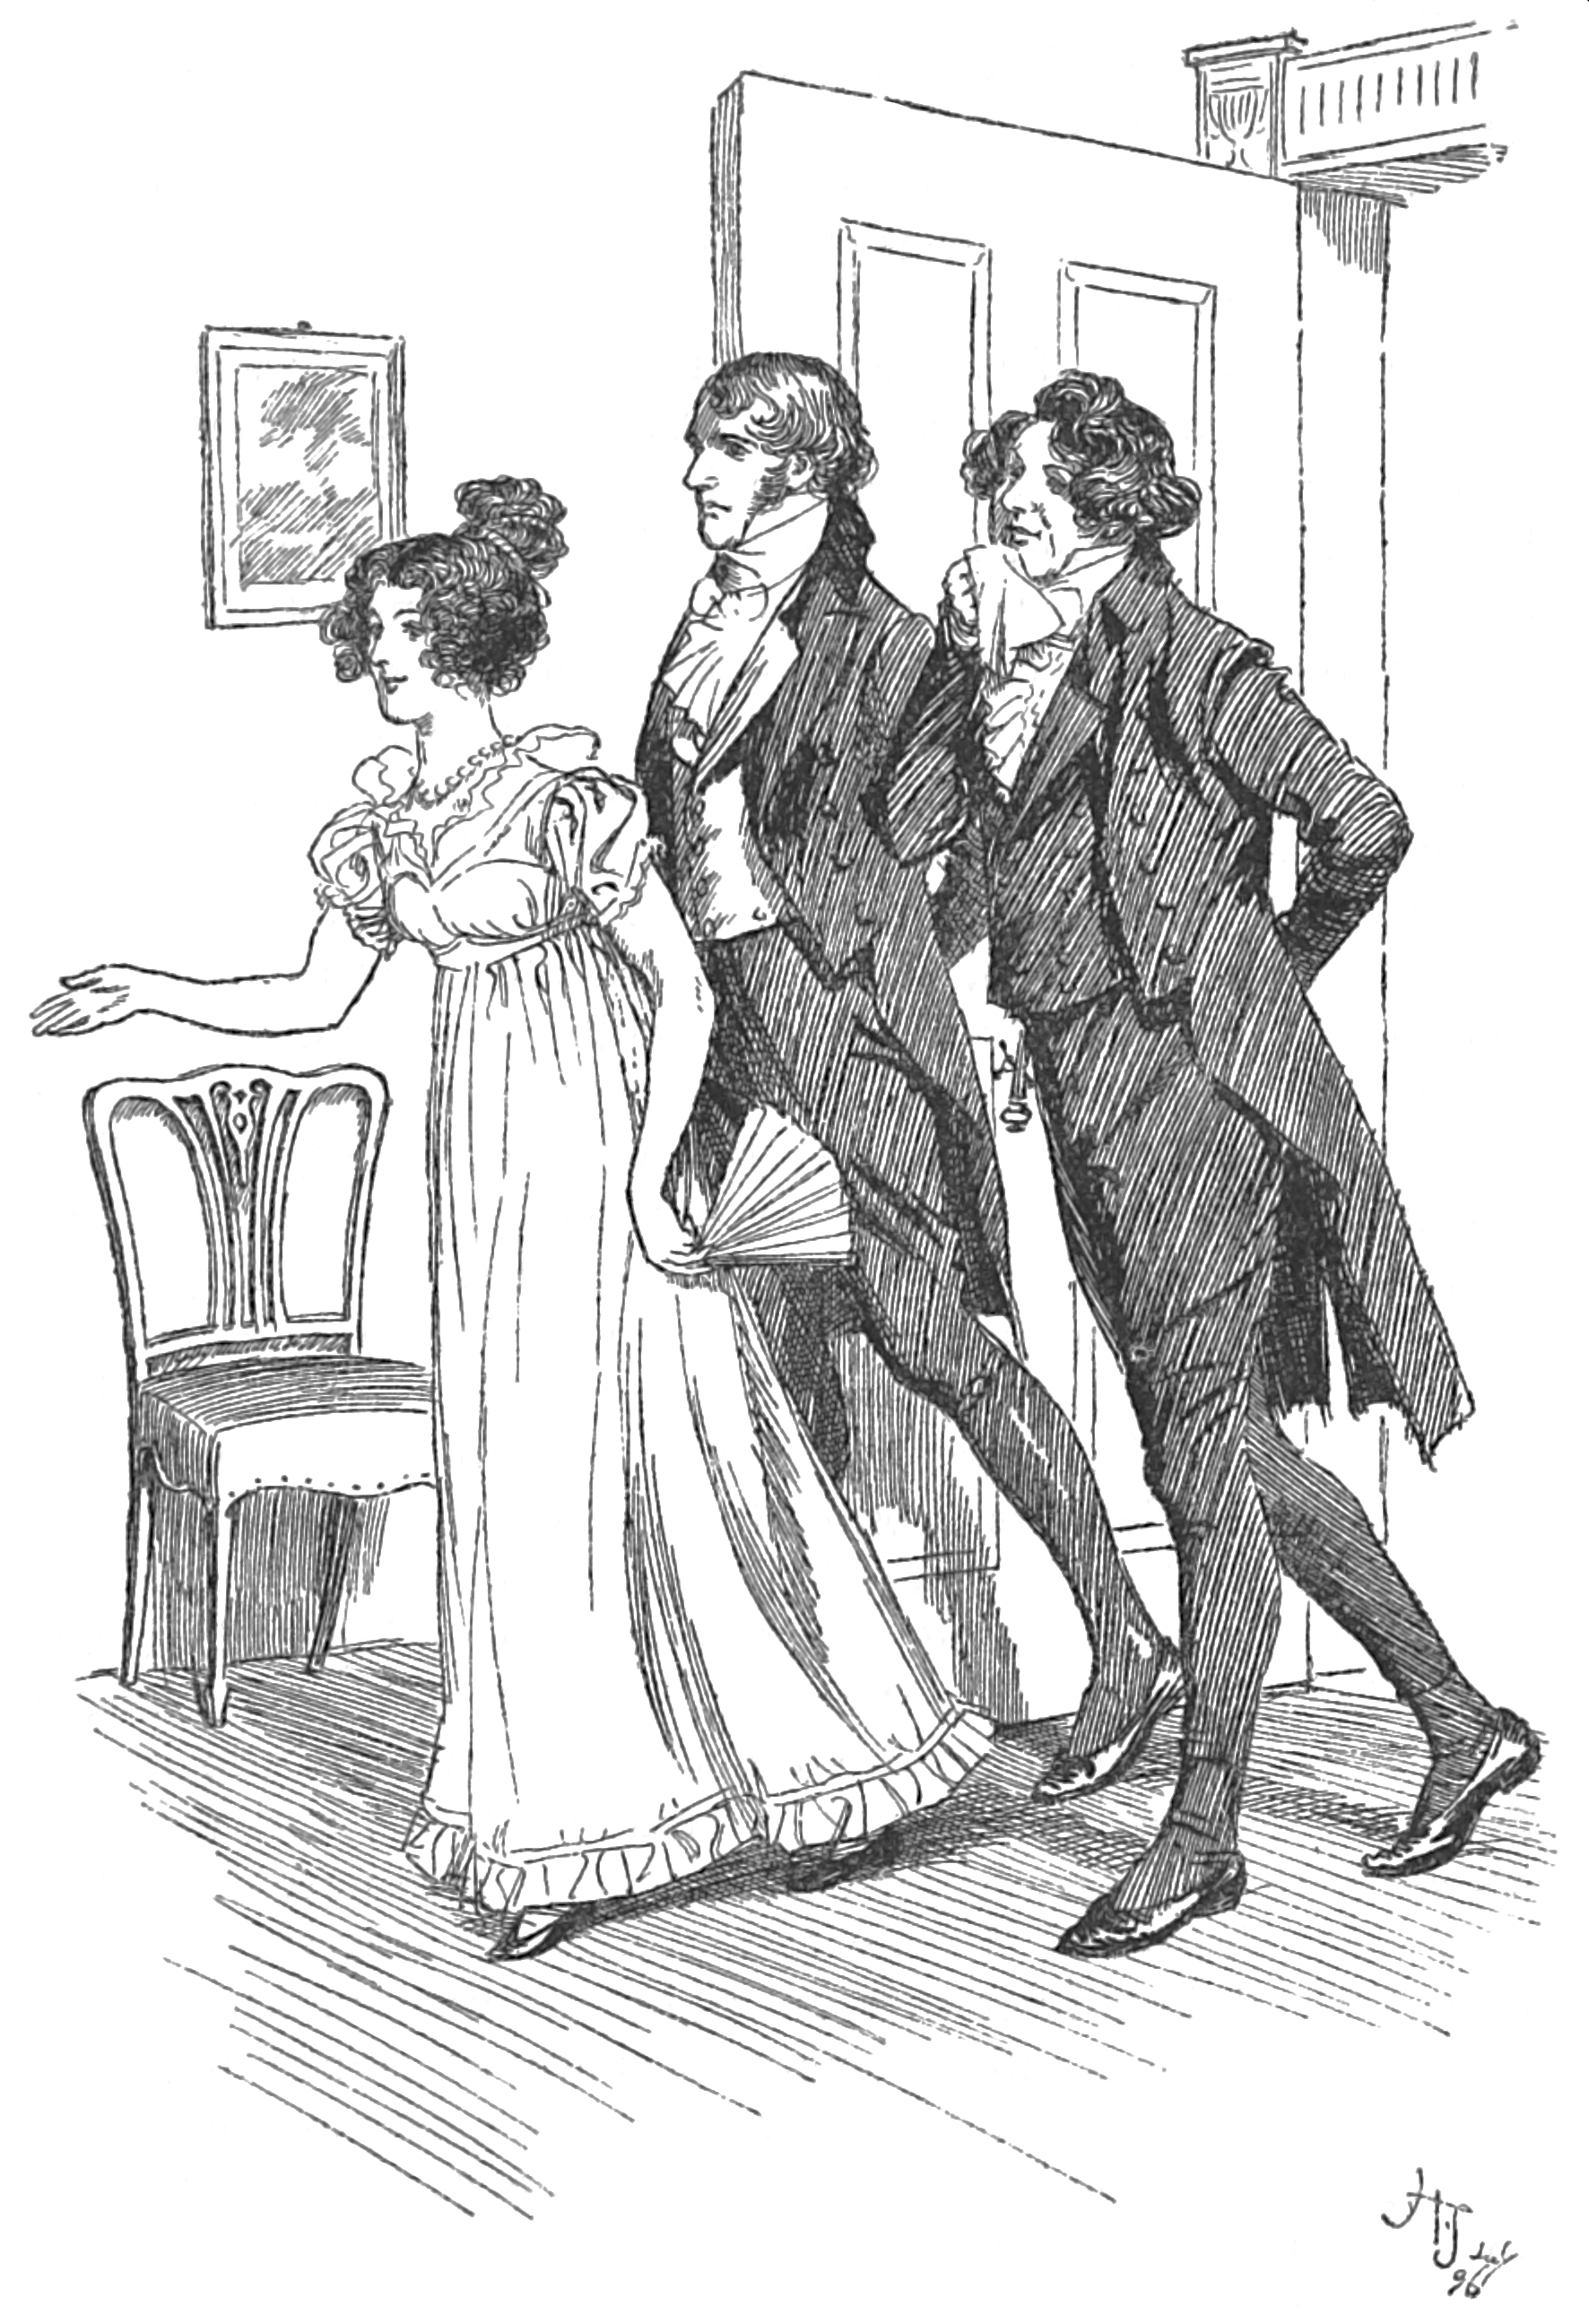
\includegraphics[width=.8\linewidth]{14drawingroom}
\caption{They walked into Mrs Weston's drawing-room}
\end{figure}

This was a pleasure which perhaps the whole day's visit might not afford, which certainly did not belong to the present half-hour; but the very sight of Mrs Weston, her smile, her touch, her voice was grateful to Emma, and she determined to think as little as possible of Mr Elton's oddities, or of any thing else unpleasant, and enjoy all that was enjoyable to the utmost.

The misfortune of Harriet's cold had been pretty well gone through before her arrival. Mr Woodhouse had been safely seated long enough to give the history of it, besides all the history of his own and Isabella's coming, and of Emma's being to follow, and had indeed just got to the end of his satisfaction that James should come and see his daughter, when the others appeared, and Mrs Weston, who had been almost wholly engrossed by her attentions to him, was able to turn away and welcome her dear Emma.

Emma's project of forgetting Mr Elton for a while made her rather sorry to find, when they had all taken their places, that he was close to her. The difficulty was great of driving his strange insensibility towards Harriet, from her mind, while he not only sat at her elbow, but was continually obtruding his happy countenance on her notice, and solicitously addressing her upon every occasion. Instead of forgetting him, his behaviour was such that she could not avoid the internal suggestion of »Can it really be as my brother imagined? can it be possible for this man to be beginning to transfer his affections from Harriet to me?—Absurd and insufferable!«—Yet he would be so anxious for her being perfectly warm, would be so interested about her father, and so delighted with Mrs Weston; and at last would begin admiring her drawings with so much zeal and so little knowledge as seemed terribly like a would-be lover, and made it some effort with her to preserve her good manners. For her own sake she could not be rude; and for Harriet's, in the hope that all would yet turn out right, she was even positively civil; but it was an effort; especially as something was going on amongst the others, in the most overpowering period of Mr Elton's nonsense, which she particularly wished to listen to. She heard enough to know that Mr Weston was giving some information about his son; she heard the words »my son,« and »Frank,« and »my son,« repeated several times over; and, from a few other half-syllables very much suspected that he was announcing an early visit from his son; but before she could quiet Mr Elton, the subject was so completely past that any reviving question from her would have been awkward.

Now, it so happened that in spite of Emma's resolution of never marrying, there was something in the name, in the idea of Mr Frank Churchill, which always interested her. She had frequently thought—especially since his father's marriage with Miss Taylor—that if she were to marry, he was the very person to suit her in age, character and condition. He seemed by this connexion between the families, quite to belong to her. She could not but suppose it to be a match that every body who knew them must think of. That Mr and Mrs Weston did think of it, she was very strongly persuaded; and though not meaning to be induced by him, or by any body else, to give up a situation which she believed more replete with good than any she could change it for, she had a great curiosity to see him, a decided intention of finding him pleasant, of being liked by him to a certain degree, and a sort of pleasure in the idea of their being coupled in their friends' imaginations.

With such sensations, Mr Elton's civilities were dreadfully ill-timed; but she had the comfort of appearing very polite, while feeling very cross—and of thinking that the rest of the visit could not possibly pass without bringing forward the same information again, or the substance of it, from the open-hearted Mr Weston.—So it proved;—for when happily released from Mr Elton, and seated by Mr Weston, at dinner, he made use of the very first interval in the cares of hospitality, the very first leisure from the saddle of mutton, to say to her,

»We want only two more to be just the right number. I should like to see two more here,—your pretty little friend, Miss Smith, and my son—and then I should say we were quite complete. I believe you did not hear me telling the others in the drawing-room that we are expecting Frank. I had a letter from him this morning, and he will be with us within a fortnight.«

Emma spoke with a very proper degree of pleasure; and fully assented to his proposition of Mr Frank Churchill and Miss Smith making their party quite complete.

»He has been wanting to come to us,« continued Mr Weston, »ever since September: every letter has been full of it; but he cannot command his own time. He has those to please who must be pleased, and who (between ourselves) are sometimes to be pleased only by a good many sacrifices. But now I have no doubt of seeing him here about the second week in January.«

»What a very great pleasure it will be to you! and Mrs Weston is so anxious to be acquainted with him, that she must be almost as happy as yourself.«

»Yes, she would be, but that she thinks there will be another put-off. She does not depend upon his coming so much as I do: but she does not know the parties so well as I do. The case, you see, is—(but this is quite between ourselves: I did not mention a syllable of it in the other room. There are secrets in all families, you know)—The case is, that a party of friends are invited to pay a visit at Enscombe in January; and that Frank's coming depends upon their being put off. If they are not put off, he cannot stir. But I know they will, because it is a family that a certain lady, of some consequence, at Enscombe, has a particular dislike to: and though it is thought necessary to invite them once in two or three years, they always are put off when it comes to the point. I have not the smallest doubt of the issue. I am as confident of seeing Frank here before the middle of January, as I am of being here myself: but your good friend there (nodding towards the upper end of the table) has so few vagaries herself, and has been so little used to them at Hartfield, that she cannot calculate on their effects, as I have been long in the practice of doing.«

»I am sorry there should be any thing like doubt in the case,« replied Emma; »but am disposed to side with you, Mr Weston. If you think he will come, I shall think so too; for you know Enscombe.«

»Yes—I have some right to that knowledge; though I have never been at the place in my life.—She is an odd woman!—But I never allow myself to speak ill of her, on Frank's account; for I do believe her to be very fond of him. I used to think she was not capable of being fond of any body, except herself: but she has always been kind to him (in her way—allowing for little whims and caprices, and expecting every thing to be as she likes). And it is no small credit, in my opinion, to him, that he should excite such an affection; for, though I would not say it to any body else, she has no more heart than a stone to people in general; and the devil of a temper.«

Emma liked the subject so well, that she began upon it, to Mrs Weston, very soon after their moving into the drawing-room: wishing her joy—yet observing, that she knew the first meeting must be rather alarming.— Mrs Weston agreed to it; but added, that she should be very glad to be secure of undergoing the anxiety of a first meeting at the time talked of: »for I cannot depend upon his coming. I cannot be so sanguine as Mr Weston. I am very much afraid that it will all end in nothing. Mr Weston, I dare say, has been telling you exactly how the matter stands?«

»Yes—it seems to depend upon nothing but the ill-humour of Mrs Churchill, which I imagine to be the most certain thing in the world.«

»My Emma!« replied Mrs Weston, smiling, »what is the certainty of caprice?« Then turning to Isabella, who had not been attending before—»You must know, my dear Mrs Knightley, that we are by no means so sure of seeing Mr Frank Churchill, in my opinion, as his father thinks. It depends entirely upon his aunt's spirits and pleasure; in short, upon her temper. To you—to my two daughters—I may venture on the truth. Mrs Churchill rules at Enscombe, and is a very odd-tempered woman; and his coming now, depends upon her being willing to spare him.«

»Oh, Mrs Churchill; every body knows Mrs Churchill,« replied Isabella: »and I am sure I never think of that poor young man without the greatest compassion. To be constantly living with an ill-tempered person, must be dreadful. It is what we happily have never known any thing of; but it must be a life of misery. What a blessing, that she never had any children! Poor little creatures, how unhappy she would have made them!«

Emma wished she had been alone with Mrs Weston. She should then have heard more: Mrs Weston would speak to her, with a degree of unreserve which she would not hazard with Isabella; and, she really believed, would scarcely try to conceal any thing relative to the Churchills from her, excepting those views on the young man, of which her own imagination had already given her such instinctive knowledge. But at present there was nothing more to be said. Mr Woodhouse very soon followed them into the drawing-room. To be sitting long after dinner, was a confinement that he could not endure. Neither wine nor conversation was any thing to him; and gladly did he move to those with whom he was always comfortable.

While he talked to Isabella, however, Emma found an opportunity of saying,

»And so you do not consider this visit from your son as by any means certain. I am sorry for it. The introduction must be unpleasant, whenever it takes place; and the sooner it could be over, the better.«

»Yes; and every delay makes one more apprehensive of other delays. Even if this family, the Braithwaites, are put off, I am still afraid that some excuse may be found for disappointing us. I cannot bear to imagine any reluctance on his side; but I am sure there is a great wish on the Churchills' to keep him to themselves. There is jealousy. They are jealous even of his regard for his father. In short, I can feel no dependence on his coming, and I wish Mr Weston were less sanguine.«

»He ought to come,« said Emma. »If he could stay only a couple of days, he ought to come; and one can hardly conceive a young man's not having it in his power to do as much as that. A young woman, if she fall into bad hands, may be teased, and kept at a distance from those she wants to be with; but one cannot comprehend a young man's being under such restraint, as not to be able to spend a week with his father, if he likes it.«

»One ought to be at Enscombe, and know the ways of the family, before one decides upon what he can do,« replied Mrs Weston. »One ought to use the same caution, perhaps, in judging of the conduct of any one individual of any one family; but Enscombe, I believe, certainly must not be judged by general rules: she is so very unreasonable; and every thing gives way to her.«

»But she is so fond of the nephew: he is so very great a favourite. Now, according to my idea of Mrs Churchill, it would be most natural, that while she makes no sacrifice for the comfort of the husband, to whom she owes every thing, while she exercises incessant caprice towards him, she should frequently be governed by the nephew, to whom she owes nothing at all.«

»My dearest Emma, do not pretend, with your sweet temper, to understand a bad one, or to lay down rules for it: you must let it go its own way. I have no doubt of his having, at times, considerable influence; but it may be perfectly impossible for him to know beforehand when it will be.«

Emma listened, and then coolly said, »I shall not be satisfied, unless he comes.«

»He may have a great deal of influence on some points,« continued Mrs Weston, »and on others, very little: and among those, on which she is beyond his reach, it is but too likely, may be this very circumstance of his coming away from them to visit us.«
%!TeX root=../emmatop.tex
\chapter[Chapter \thechapter]{}
\lettrine[lines=4,lraise=0.3]{M}{r} Woodhouse was soon ready for his tea; and when he had drank his tea he was quite ready to go home; and it was as much as his three companions could do, to entertain away his notice of the lateness of the hour, before the other gentlemen appeared. Mr Weston was chatty and convivial, and no friend to early separations of any sort; but at last the drawing-room party did receive an augmentation. Mr Elton, in very good spirits, was one of the first to walk in. Mrs Weston and Emma were sitting together on a sofa. He joined them immediately, and, with scarcely an invitation, seated himself between them.

Emma, in good spirits too, from the amusement afforded her mind by the expectation of Mr Frank Churchill, was willing to forget his late improprieties, and be as well satisfied with him as before, and on his making Harriet his very first subject, was ready to listen with most friendly smiles.

He professed himself extremely anxious about her fair friend—her fair, lovely, amiable friend. »Did she know?—had she heard any thing about her, since their being at Randalls?—he felt much anxiety—he must confess that the nature of her complaint alarmed him considerably.« And in this style he talked on for some time very properly, not much attending to any answer, but altogether sufficiently awake to the terror of a bad sore throat; and Emma was quite in charity with him.

But at last there seemed a perverse turn; it seemed all at once as if he were more afraid of its being a bad sore throat on her account, than on Harriet's—more anxious that she should escape the infection, than that there should be no infection in the complaint. He began with great earnestness to entreat her to refrain from visiting the sick-chamber again, for the present—to entreat her to promise him not to venture into such hazard till he had seen Mr Perry and learnt his opinion; and though she tried to laugh it off and bring the subject back into its proper course, there was no putting an end to his extreme solicitude about her. She was vexed. It did appear—there was no concealing it—exactly like the pretence of being in love with her, instead of Harriet; an inconstancy, if real, the most contemptible and abominable! and she had difficulty in behaving with temper. He turned to Mrs Weston to implore her assistance, »Would not she give him her support?—would not she add her persuasions to his, to induce Miss Woodhouse not to go to Mrs Goddard's till it were certain that Miss Smith's disorder had no infection? He could not be satisfied without a promise—would not she give him her influence in procuring it?«

\begin{figure}[tbph]
\centering
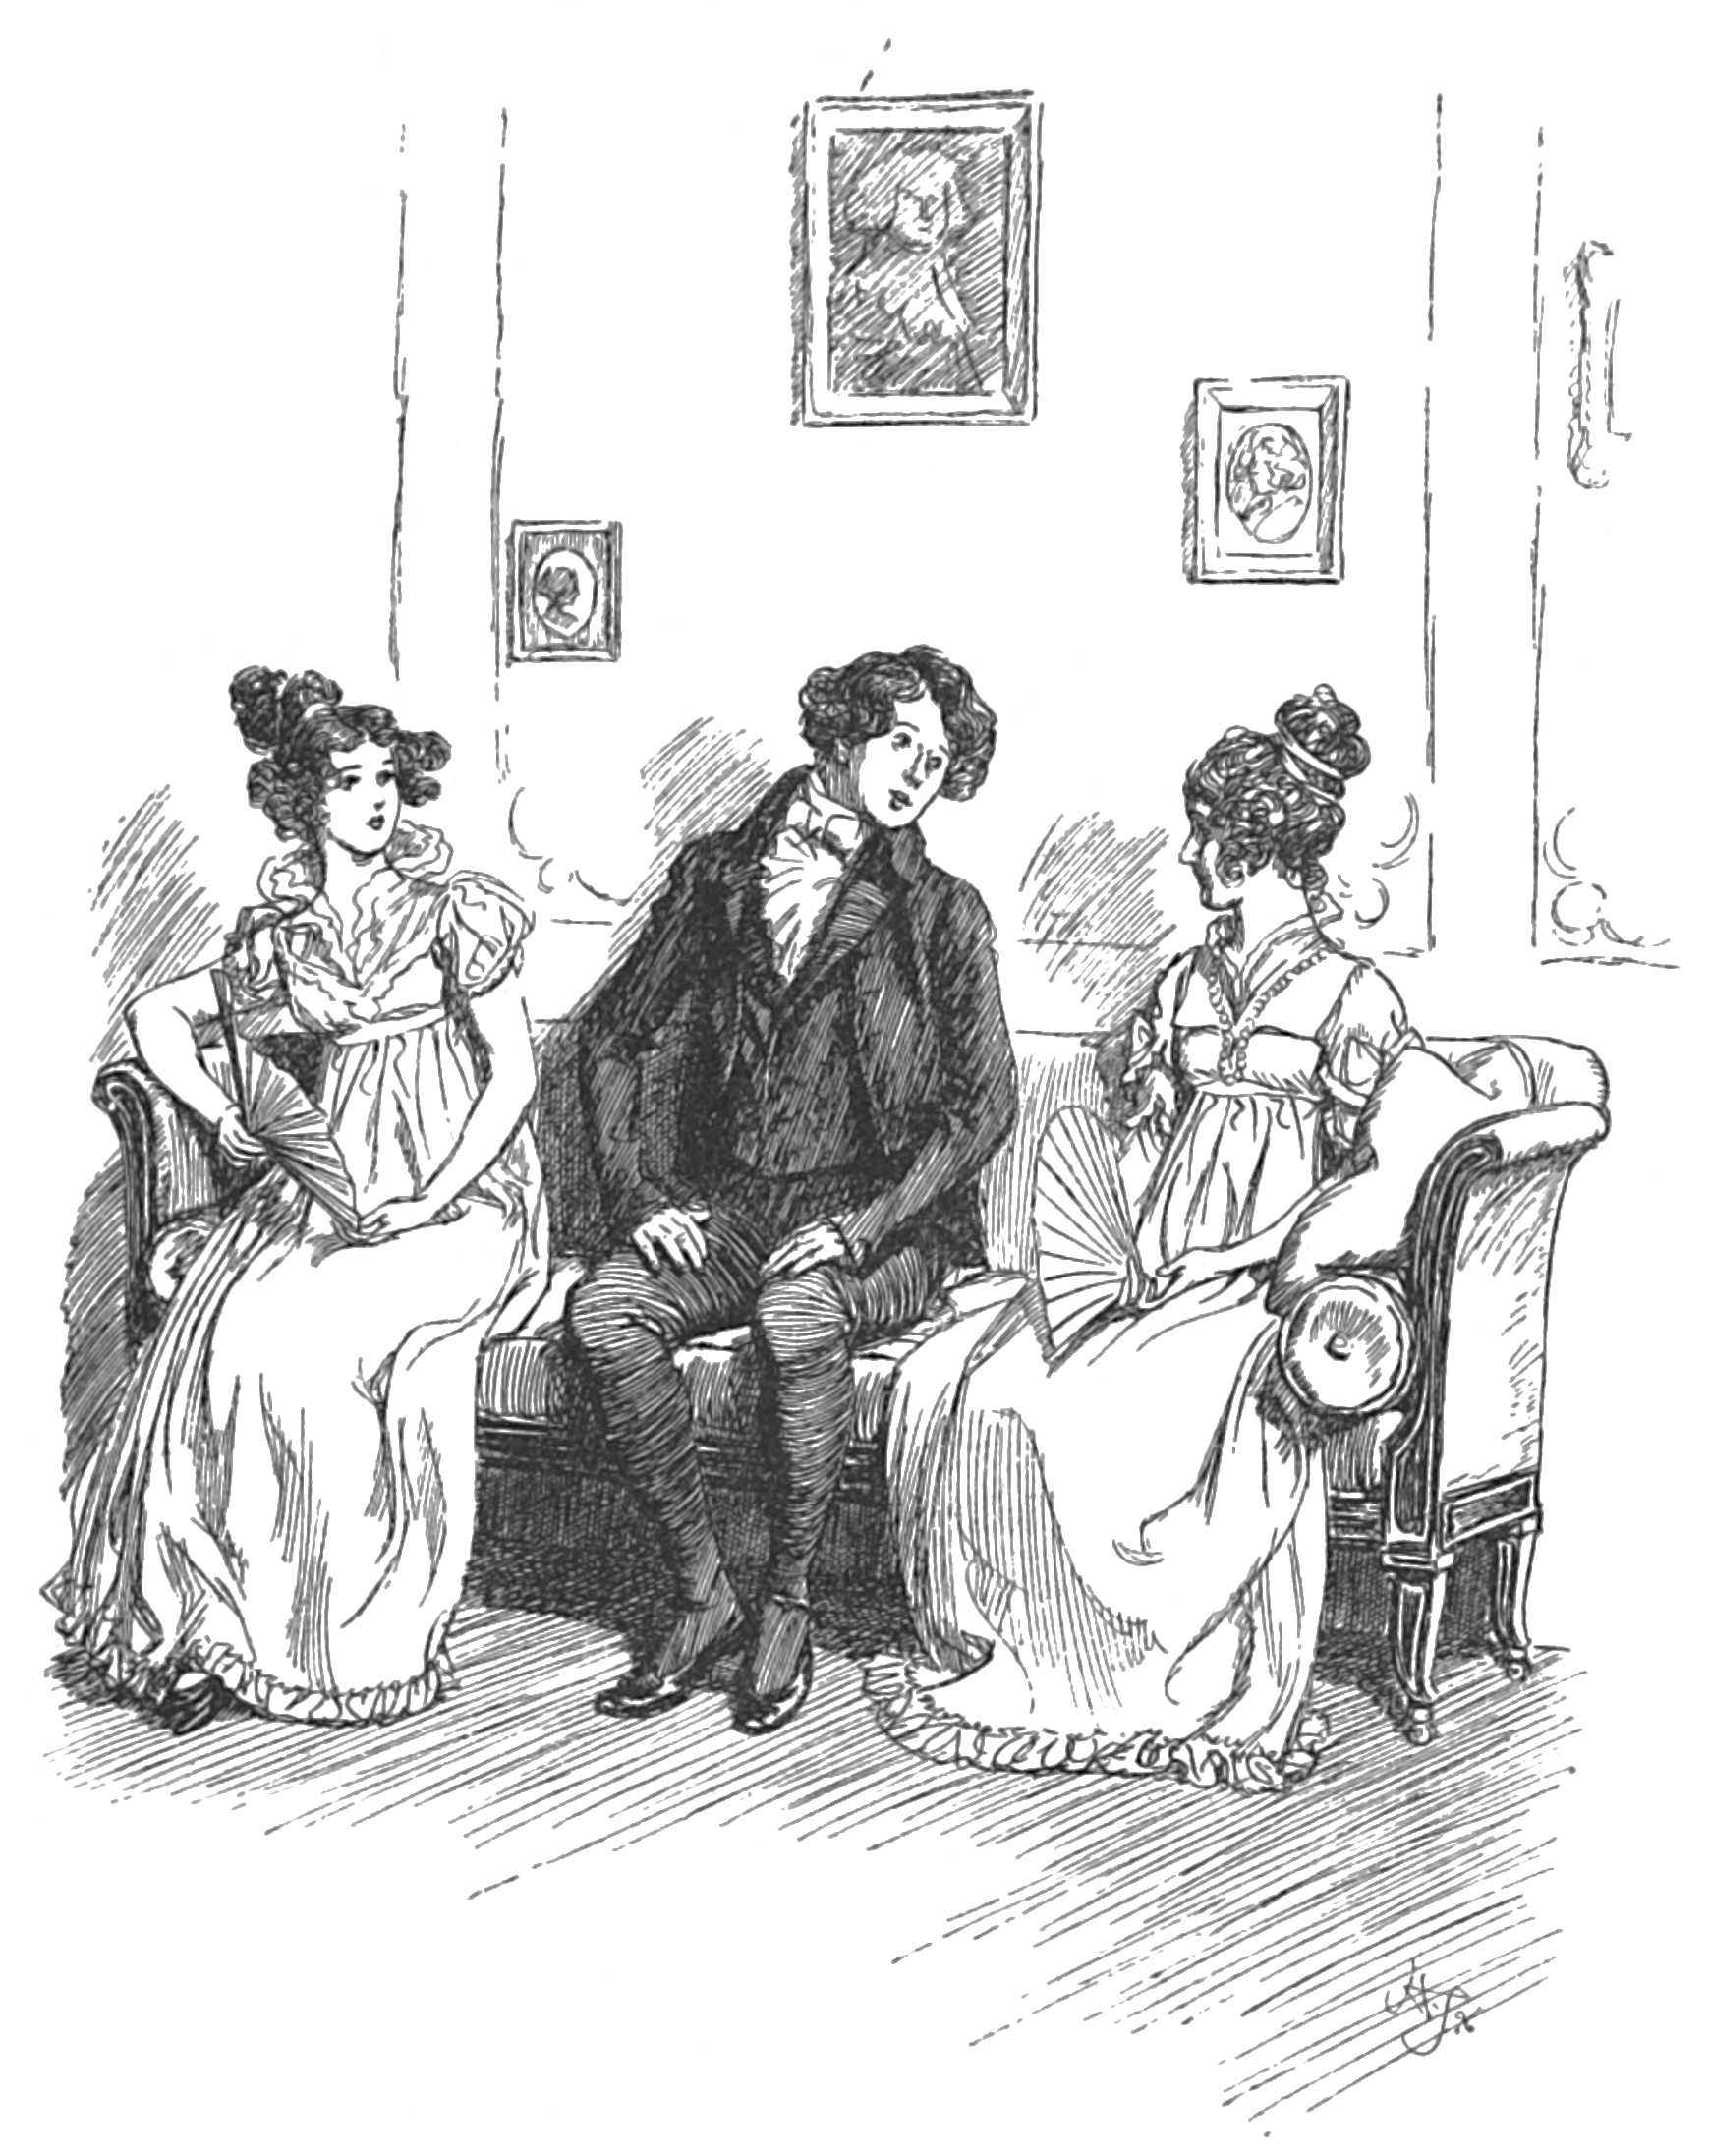
\includegraphics[width=.9\linewidth]{15fair}
\caption{»Is this fair, Mrs Weston?«}
\end{figure}

»So scrupulous for others,« he continued, »and yet so careless for herself! She wanted me to nurse my cold by staying at home to-day, and yet will not promise to avoid the danger of catching an ulcerated sore throat herself. Is this fair, Mrs Weston?—Judge between us. Have not I some right to complain? I am sure of your kind support and aid.«

Emma saw Mrs Weston's surprize, and felt that it must be great, at an address which, in words and manner, was assuming to himself the right of first interest in her; and as for herself, she was too much provoked and offended to have the power of directly saying any thing to the purpose. She could only give him a look; but it was such a look as she thought must restore him to his senses, and then left the sofa, removing to a seat by her sister, and giving her all her attention.

She had not time to know how Mr Elton took the reproof, so rapidly did another subject succeed; for Mr John Knightley now came into the room from examining the weather, and opened on them all with the information of the ground being covered with snow, and of its still snowing fast, with a strong drifting wind; concluding with these words to Mr Woodhouse:

»This will prove a spirited beginning of your winter engagements, sir. Something new for your coachman and horses to be making their way through a storm of snow.«

Poor Mr Woodhouse was silent from consternation; but every body else had something to say; every body was either surprized or not surprized, and had some question to ask, or some comfort to offer. Mrs Weston and Emma tried earnestly to cheer him and turn his attention from his son-in-law, who was pursuing his triumph rather unfeelingly.

»I admired your resolution very much, sir,« said he, »in venturing out in such weather, for of course you saw there would be snow very soon. Every body must have seen the snow coming on. I admired your spirit; and I dare say we shall get home very well. Another hour or two's snow can hardly make the road impassable; and we are two carriages; if one is blown over in the bleak part of the common field there will be the other at hand. I dare say we shall be all safe at Hartfield before midnight.«

Mr Weston, with triumph of a different sort, was confessing that he had known it to be snowing some time, but had not said a word, lest it should make Mr Woodhouse uncomfortable, and be an excuse for his hurrying away. As to there being any quantity of snow fallen or likely to fall to impede their return, that was a mere joke; he was afraid they would find no difficulty. He wished the road might be impassable, that he might be able to keep them all at Randalls; and with the utmost good-will was sure that accommodation might be found for every body, calling on his wife to agree with him, that with a little contrivance, every body might be lodged, which she hardly knew how to do, from the consciousness of there being but two spare rooms in the house.

»What is to be done, my dear Emma?—what is to be done?« was Mr Woodhouse's first exclamation, and all that he could say for some time. To her he looked for comfort; and her assurances of safety, her representation of the excellence of the horses, and of James, and of their having so many friends about them, revived him a little.

His eldest daughter's alarm was equal to his own. The horror of being blocked up at Randalls, while her children were at Hartfield, was full in her imagination; and fancying the road to be now just passable for adventurous people, but in a state that admitted no delay, she was eager to have it settled, that her father and Emma should remain at Randalls, while she and her husband set forward instantly through all the possible accumulations of drifted snow that might impede them.

»You had better order the carriage directly, my love,« said she; »I dare say we shall be able to get along, if we set off directly; and if we do come to any thing very bad, I can get out and walk. I am not at all afraid. I should not mind walking half the way. I could change my shoes, you know, the moment I got home; and it is not the sort of thing that gives me cold.«

»Indeed!« replied he. »Then, my dear Isabella, it is the most extraordinary sort of thing in the world, for in general every thing does give you cold. Walk home!—you are prettily shod for walking home, I dare say. It will be bad enough for the horses.«

Isabella turned to Mrs Weston for her approbation of the plan. Mrs Weston could only approve. Isabella then went to Emma; but Emma could not so entirely give up the hope of their being all able to get away; and they were still discussing the point, when Mr Knightley, who had left the room immediately after his brother's first report of the snow, came back again, and told them that he had been out of doors to examine, and could answer for there not being the smallest difficulty in their getting home, whenever they liked it, either now or an hour hence. He had gone beyond the sweep—some way along the Highbury road—the snow was nowhere above half an inch deep—in many places hardly enough to whiten the ground; a very few flakes were falling at present, but the clouds were parting, and there was every appearance of its being soon over. He had seen the coachmen, and they both agreed with him in there being nothing to apprehend.

To Isabella, the relief of such tidings was very great, and they were scarcely less acceptable to Emma on her father's account, who was immediately set as much at ease on the subject as his nervous constitution allowed; but the alarm that had been raised could not be appeased so as to admit of any comfort for him while he continued at Randalls. He was satisfied of there being no present danger in returning home, but no assurances could convince him that it was safe to stay; and while the others were variously urging and recommending, Mr Knightley and Emma settled it in a few brief sentences: thus—

»Your father will not be easy; why do not you go?«

»I am ready, if the others are.«

»Shall I ring the bell?«

»Yes, do.«

And the bell was rung, and the carriages spoken for. A few minutes more, and Emma hoped to see one troublesome companion deposited in his own house, to get sober and cool, and the other recover his temper and happiness when this visit of hardship were over.

The carriage came: and Mr Woodhouse, always the first object on such occasions, was carefully attended to his own by Mr Knightley and Mr Weston; but not all that either could say could prevent some renewal of alarm at the sight of the snow which had actually fallen, and the discovery of a much darker night than he had been prepared for. »He was afraid they should have a very bad drive. He was afraid poor Isabella would not like it. And there would be poor Emma in the carriage behind. He did not know what they had best do. They must keep as much together as they could;« and James was talked to, and given a charge to go very slow and wait for the other carriage.

Isabella stept in after her father; John Knightley, forgetting that he did not belong to their party, stept in after his wife very naturally; so that Emma found, on being escorted and followed into the second carriage by Mr Elton, that the door was to be lawfully shut on them, and that they were to have a tête-à-tête drive. It would not have been the awkwardness of a moment, it would have been rather a pleasure, previous to the suspicions of this very day; she could have talked to him of Harriet, and the three-quarters of a mile would have seemed but one. But now, she would rather it had not happened. She believed he had been drinking too much of Mr Weston's good wine, and felt sure that he would want to be talking nonsense.

To restrain him as much as might be, by her own manners, she was immediately preparing to speak with exquisite calmness and gravity of the weather and the night; but scarcely had she begun, scarcely had they passed the sweep-gate and joined the other carriage, than she found her subject cut up—her hand seized—her attention demanded, and Mr Elton actually making violent love to her: availing himself of the precious opportunity, declaring sentiments which must be already well known, hoping—fearing—adoring—ready to die if she refused him; but flattering himself that his ardent attachment and unequalled love and unexampled passion could not fail of having some effect, and in short, very much resolved on being seriously accepted as soon as possible. It really was so. Without scruple—without apology—without much apparent diffidence, Mr Elton, the lover of Harriet, was professing himself her lover. She tried to stop him; but vainly; he would go on, and say it all. Angry as she was, the thought of the moment made her resolve to restrain herself when she did speak. She felt that half this folly must be drunkenness, and therefore could hope that it might belong only to the passing hour. Accordingly, with a mixture of the serious and the playful, which she hoped would best suit his half and half state, she replied,

»I am very much astonished, Mr Elton. This to me! you forget yourself—you take me for my friend—any message to Miss Smith I shall be happy to deliver; but no more of this to me, if you please.«

»Miss Smith!—message to Miss Smith!—What could she possibly mean!«—And he repeated her words with such assurance of accent, such boastful pretence of amazement, that she could not help replying with quickness,

»Mr Elton, this is the most extraordinary conduct! and I can account for it only in one way; you are not yourself, or you could not speak either to me, or of Harriet, in such a manner. Command yourself enough to say no more, and I will endeavour to forget it.«

But Mr Elton had only drunk wine enough to elevate his spirits, not at all to confuse his intellects. He perfectly knew his own meaning; and having warmly protested against her suspicion as most injurious, and slightly touched upon his respect for Miss Smith as her friend,—but acknowledging his wonder that Miss Smith should be mentioned at all,—he resumed the subject of his own passion, and was very urgent for a favourable answer.

As she thought less of his inebriety, she thought more of his inconstancy and presumption; and with fewer struggles for politeness, replied,

»It is impossible for me to doubt any longer. You have made yourself too clear. Mr Elton, my astonishment is much beyond any thing I can express. After such behaviour, as I have witnessed during the last month, to Miss Smith—such attentions as I have been in the daily habit of observing—to be addressing me in this manner—this is an unsteadiness of character, indeed, which I had not supposed possible! Believe me, sir, I am far, very far, from gratified in being the object of such professions.«

»Good Heaven!« cried Mr Elton, »what can be the meaning of this?—Miss Smith!—I never thought of Miss Smith in the whole course of my existence—never paid her any attentions, but as your friend: never cared whether she were dead or alive, but as your friend. If she has fancied otherwise, her own wishes have misled her, and I am very sorry—extremely sorry—But, Miss Smith, indeed!—Oh! Miss Woodhouse! who can think of Miss Smith, when Miss Woodhouse is near! No, upon my honour, there is no unsteadiness of character. I have thought only of you. I protest against having paid the smallest attention to any one else. Every thing that I have said or done, for many weeks past, has been with the sole view of marking my adoration of yourself. You cannot really, seriously, doubt it. No!—(in an accent meant to be insinuating)—I am sure you have seen and understood me.«

It would be impossible to say what Emma felt, on hearing this—which of all her unpleasant sensations was uppermost. She was too completely overpowered to be immediately able to reply: and two moments of silence being ample encouragement for Mr Elton's sanguine state of mind, he tried to take her hand again, as he joyously exclaimed—

»Charming Miss Woodhouse! allow me to interpret this interesting silence. It confesses that you have long understood me.«

»No, sir,« cried Emma, »it confesses no such thing. So far from having long understood you, I have been in a most complete error with respect to your views, till this moment. As to myself, I am very sorry that you should have been giving way to any feelings—Nothing could be farther from my wishes—your attachment to my friend Harriet—your pursuit of her, (pursuit, it appeared,) gave me great pleasure, and I have been very earnestly wishing you success: but had I supposed that she were not your attraction to Hartfield, I should certainly have thought you judged ill in making your visits so frequent. Am I to believe that you have never sought to recommend yourself particularly to Miss Smith?—that you have never thought seriously of her?«

»Never, madam,« cried he, affronted in his turn: »never, I assure you. I think seriously of Miss Smith!—Miss Smith is a very good sort of girl; and I should be happy to see her respectably settled. I wish her extremely well: and, no doubt, there are men who might not object to—Every body has their level: but as for myself, I am not, I think, quite so much at a loss. I need not so totally despair of an equal alliance, as to be addressing myself to Miss Smith!—No, madam, my visits to Hartfield have been for yourself only; and the encouragement I received\longdash«

»Encouragement!—I give you encouragement!—Sir, you have been entirely mistaken in supposing it. I have seen you only as the admirer of my friend. In no other light could you have been more to me than a common acquaintance. I am exceedingly sorry: but it is well that the mistake ends where it does. Had the same behaviour continued, Miss Smith might have been led into a misconception of your views; not being aware, probably, any more than myself, of the very great inequality which you are so sensible of. But, as it is, the disappointment is single, and, I trust, will not be lasting. I have no thoughts of matrimony at present.«

He was too angry to say another word; her manner too decided to invite supplication; and in this state of swelling resentment, and mutually deep mortification, they had to continue together a few minutes longer, for the fears of Mr Woodhouse had confined them to a foot-pace. If there had not been so much anger, there would have been desperate awkwardness; but their straightforward emotions left no room for the little zigzags of embarrassment. Without knowing when the carriage turned into Vicarage Lane, or when it stopped, they found themselves, all at once, at the door of his house; and he was out before another syllable passed.—Emma then felt it indispensable to wish him a good night. The compliment was just returned, coldly and proudly; and, under indescribable irritation of spirits, she was then conveyed to Hartfield.

There she was welcomed, with the utmost delight, by her father, who had been trembling for the dangers of a solitary drive from Vicarage Lane—turning a corner which he could never bear to think of—and in strange hands—a mere common coachman—no James; and there it seemed as if her return only were wanted to make every thing go well: for Mr John Knightley, ashamed of his ill-humour, was now all kindness and attention; and so particularly solicitous for the comfort of her father, as to seem—if not quite ready to join him in a basin of gruel—perfectly sensible of its being exceedingly wholesome; and the day was concluding in peace and comfort to all their little party, except herself.—But her mind had never been in such perturbation; and it needed a very strong effort to appear attentive and cheerful till the usual hour of separating allowed her the relief of quiet reflection.
%!TeX root=../sensetop.tex
\chapter[Chapter \thechapter]{}
\lettrine[lraise=0.3]{M}{arianne} would have thought herself very inexcusable had she been able to sleep at all the first night after parting from Willoughby. She would have been ashamed to look her family in the face the next morning, had she not risen from her bed in more need of repose than when she lay down in it. But the feelings which made such composure a disgrace, left her in no danger of incurring it. She was awake the whole night, and she wept the greatest part of it. She got up with a headache, was unable to talk, and unwilling to take any nourishment; giving pain every moment to her mother and sisters, and forbidding all attempt at consolation from either. Her sensibility was potent enough!

When breakfast was over she walked out by herself, and wandered about the village of Allenham, indulging the recollection of past enjoyment and crying over the present reverse for the chief of the morning.

The evening passed off in the equal indulgence of feeling. She played over every favourite song that she had been used to play to Willoughby, every air in which their voices had been oftenest joined, and sat at the instrument gazing on every line of music that he had written out for her, till her heart was so heavy that no farther sadness could be gained; and this nourishment of grief was every day applied. She spent whole hours at the pianoforte alternately singing and crying; her voice often totally suspended by her tears. In books too, as well as in music, she courted the misery which a contrast between the past and present was certain of giving. She read nothing but what they had been used to read together.

Such violence of affliction indeed could not be supported for ever; it sunk within a few days into a calmer melancholy; but these employments, to which she daily recurred, her solitary walks and silent meditations, still produced occasional effusions of sorrow as lively as ever.

No letter from Willoughby came; and none seemed expected by Marianne. Her mother was surprised, and Elinor again became uneasy. But Mrs Dashwood could find explanations whenever she wanted them, which at least satisfied herself.

<Remember, Elinor,> said she, <how very often Sir John fetches our letters himself from the post, and carries them to it. We have already agreed that secrecy may be necessary, and we must acknowledge that it could not be maintained if their correspondence were to pass through Sir John's hands.>

Elinor could not deny the truth of this, and she tried to find in it a motive sufficient for their silence. But there was one method so direct, so simple, and in her opinion so eligible of knowing the real state of the affair, and of instantly removing all mystery, that she could not help suggesting it to her mother.

<Why do you not ask Marianne at once,> said she, <whether she is or she is not engaged to Willoughby? From you, her mother, and so kind, so indulgent a mother, the question could not give offence. It would be the natural result of your affection for her. She used to be all unreserve, and to you more especially.>

<I would not ask such a question for the world. Supposing it possible that they are not engaged, what distress would not such an enquiry inflict! At any rate it would be most ungenerous. I should never deserve her confidence again, after forcing from her a confession of what is meant at present to be unacknowledged to any one. I know Marianne's heart: I know that she dearly loves me, and that I shall not be the last to whom the affair is made known, when circumstances make the revealment of it eligible. I would not attempt to force the confidence of any one; of a child much less; because a sense of duty would prevent the denial which her wishes might direct.>

Elinor thought this generosity overstrained, considering her sister's youth, and urged the matter farther, but in vain; common sense, common care, common prudence, were all sunk in Mrs Dashwood's romantic delicacy.

It was several days before Willoughby's name was mentioned before Marianne by any of her family; Sir John and Mrs Jennings, indeed, were not so nice; their witticisms added pain to many a painful hour;—but one evening, Mrs Dashwood, accidentally taking up a volume of Shakespeare, exclaimed,

<We have never finished \textit{Hamlet}, Marianne; our dear Willoughby went away before we could get through it. We will put it by, that when he comes again...But it may be months, perhaps, before \textit{that} happens.>

<Months!> cried Marianne, with strong surprise. <No—nor many weeks.>

Mrs Dashwood was sorry for what she had said; but it gave Elinor pleasure, as it produced a reply from Marianne so expressive of confidence in Willoughby and knowledge of his intentions.

One morning, about a week after his leaving the country, Marianne was prevailed on to join her sisters in their usual walk, instead of wandering away by herself. Hitherto she had carefully avoided every companion in her rambles. If her sisters intended to walk on the downs, she directly stole away towards the lanes; if they talked of the valley, she was as speedy in climbing the hills, and could never be found when the others set off. But at length she was secured by the exertions of Elinor, who greatly disapproved such continual seclusion. They walked along the road through the valley, and chiefly in silence, for Marianne's \textit{mind} could not be controlled, and Elinor, satisfied with gaining one point, would not then attempt more. Beyond the entrance of the valley, where the country, though still rich, was less wild and more open, a long stretch of the road which they had travelled on first coming to Barton, lay before them; and on reaching that point, they stopped to look around them, and examine a prospect which formed the distance of their view from the cottage, from a spot which they had never happened to reach in any of their walks before.

Amongst the objects in the scene, they soon discovered an animated one; it was a man on horseback riding towards them. In a few minutes they could distinguish him to be a gentleman; and in a moment afterwards Marianne rapturously exclaimed,

<It is he; it is indeed;—I know it is!>—and was hastening to meet him, when Elinor cried out,

<Indeed, Marianne, I think you are mistaken. It is not Willoughby. The person is not tall enough for him, and has not his air.>

<He has, he has,> cried Marianne, <I am sure he has. His air, his coat, his horse. I knew how soon he would come.>

She walked eagerly on as she spoke; and Elinor, to screen Marianne from particularity, as she felt almost certain of its not being Willoughby, quickened her pace and kept up with her. They were soon within thirty yards of the gentleman. Marianne looked again; her heart sunk within her; and abruptly turning round, she was hurrying back, when the voices of both her sisters were raised to detain her; a third, almost as well known as Willoughby's, joined them in begging her to stop, and she turned round with surprise to see and welcome Edward Ferrars.

% \begin{figure}[tbph]
% \centering
% 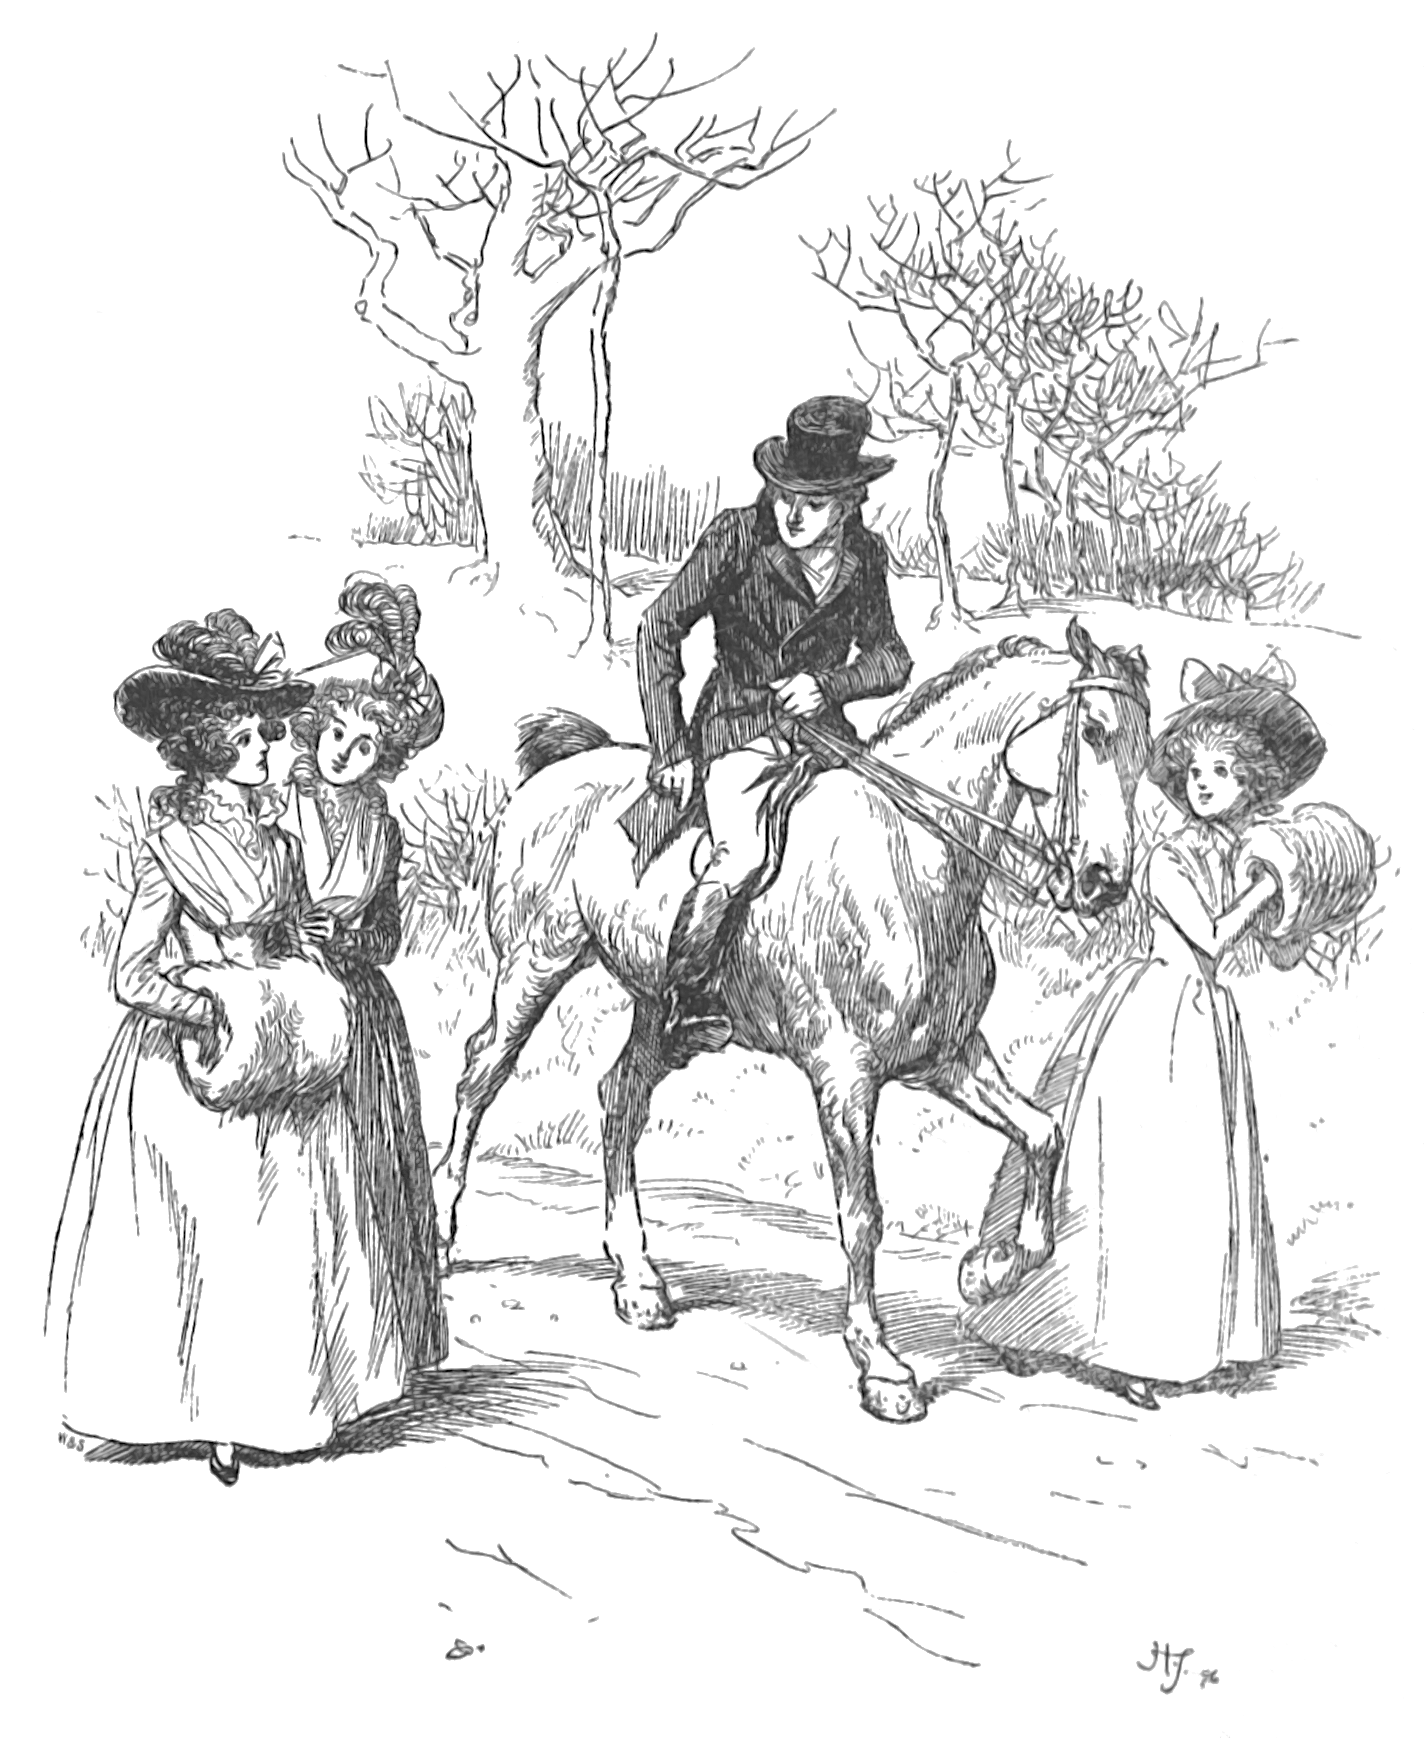
\includegraphics[width=\linewidth]{16stop}
% \caption{Begging her to stop}
% \end{figure}

\begin{bwbigpic}
	[1.0]
	{16stop} 
	{Begging her to stop} 
\end{bwbigpic}

He was the only person in the world who could at that moment be forgiven for not being Willoughby; the only one who could have gained a smile from her; but she dispersed her tears to smile on \textit{him}, and in her sister's happiness forgot for a time her own disappointment.

He dismounted, and giving his horse to his servant, walked back with them to Barton, whither he was purposely coming to visit them.

He was welcomed by them all with great cordiality, but especially by Marianne, who showed more warmth of regard in her reception of him than even Elinor herself. To Marianne, indeed, the meeting between Edward and her sister was but a continuation of that unaccountable coldness which she had often observed at Norland in their mutual behaviour. On Edward's side, more particularly, there was a deficiency of all that a lover ought to look and say on such an occasion. He was confused, seemed scarcely sensible of pleasure in seeing them, looked neither rapturous nor gay, said little but what was forced from him by questions, and distinguished Elinor by no mark of affection. Marianne saw and listened with increasing surprise. She began almost to feel a dislike of Edward; and it ended, as every feeling must end with her, by carrying back her thoughts to Willoughby, whose manners formed a contrast sufficiently striking to those of his brother elect.

After a short silence which succeeded the first surprise and enquiries of meeting, Marianne asked Edward if he came directly from London. No, he had been in Devonshire a fortnight.

<A fortnight!> she repeated, surprised at his being so long in the same county with Elinor without seeing her before.

He looked rather distressed as he added, that he had been staying with some friends near Plymouth.

<Have you been lately in Sussex?> said Elinor.

<I was at Norland about a month ago.>

<And how does dear, dear Norland look?> cried Marianne.

<Dear, dear Norland,> said Elinor, <probably looks much as it always does at this time of the year. The woods and walks thickly covered with dead leaves.>

<Oh,> cried Marianne, <with what transporting sensation have I formerly seen them fall! How have I delighted, as I walked, to see them driven in showers about me by the wind! What feelings have they, the season, the air altogether inspired! Now there is no one to regard them. They are seen only as a nuisance, swept hastily off, and driven as much as possible from the sight.>

<It is not every one,> said Elinor, <who has your passion for dead leaves.>

<No; my feelings are not often shared, not often understood. But \textit{sometimes} they are.>—As she said this, she sunk into a reverie for a few moments;—but rousing herself again, <Now, Edward,> said she, calling his attention to the prospect, <here is Barton valley. Look up to it, and be tranquil if you can. Look at those hills! Did you ever see their equals? To the left is Barton park, amongst those woods and plantations. You may see the end of the house. And there, beneath that farthest hill, which rises with such grandeur, is our cottage.>

<It is a beautiful country,> he replied; <but these bottoms must be dirty in winter.>

<How can you think of dirt, with such objects before you?>

<Because,> replied he, smiling, <among the rest of the objects before me, I see a very dirty lane.>

<How strange!> said Marianne to herself as she walked on.

<Have you an agreeable neighbourhood here? Are the Middletons pleasant people?>

<No, not all,> answered Marianne; <we could not be more unfortunately situated.>

<Marianne,> cried her sister, <how can you say so? How can you be so unjust? They are a very respectable family, Mr Ferrars; and towards us have behaved in the friendliest manner. Have you forgot, Marianne, how many pleasant days we have owed to them?>

<No,> said Marianne, in a low voice, <nor how many painful moments.>

Elinor took no notice of this; and directing her attention to their visitor, endeavoured to support something like discourse with him, by talking of their present residence, its conveniences, \&c. extorting from him occasional questions and remarks. His coldness and reserve mortified her severely; she was vexed and half angry; but resolving to regulate her behaviour to him by the past rather than the present, she avoided every appearance of resentment or displeasure, and treated him as she thought he ought to be treated from the family connection.
%!TeX root=../emmatop.tex
\chapter[Chapter \thechapter]{}
\lettrine[lines=4,lraise=0.3]{M}{r} and Mrs John Knightley were not detained long at Hartfield. The weather soon improved enough for those to move who must move; and Mr Woodhouse having, as usual, tried to persuade his daughter to stay behind with all her children, was obliged to see the whole party set off, and return to his lamentations over the destiny of poor Isabella;—which poor Isabella, passing her life with those she doated on, full of their merits, blind to their faults, and always innocently busy, might have been a model of right feminine happiness.

The evening of the very day on which they went brought a note from Mr Elton to Mr Woodhouse, a long, civil, ceremonious note, to say, with Mr Elton's best compliments, »that he was proposing to leave Highbury the following morning in his way to Bath; where, in compliance with the pressing entreaties of some friends, he had engaged to spend a few weeks, and very much regretted the impossibility he was under, from various circumstances of weather and business, of taking a personal leave of Mr Woodhouse, of whose friendly civilities he should ever retain a grateful sense—and had Mr Woodhouse any commands, should be happy to attend to them.«

Emma was most agreeably surprized.—Mr Elton's absence just at this time was the very thing to be desired. She admired him for contriving it, though not able to give him much credit for the manner in which it was announced. Resentment could not have been more plainly spoken than in a civility to her father, from which she was so pointedly excluded. She had not even a share in his opening compliments.—Her name was not mentioned;—and there was so striking a change in all this, and such an ill-judged solemnity of leave-taking in his graceful acknowledgments, as she thought, at first, could not escape her father's suspicion.

It did, however.—Her father was quite taken up with the surprize of so sudden a journey, and his fears that Mr Elton might never get safely to the end of it, and saw nothing extraordinary in his language. It was a very useful note, for it supplied them with fresh matter for thought and conversation during the rest of their lonely evening. Mr Woodhouse talked over his alarms, and Emma was in spirits to persuade them away with all her usual promptitude.

She now resolved to keep Harriet no longer in the dark. She had reason to believe her nearly recovered from her cold, and it was desirable that she should have as much time as possible for getting the better of her other complaint before the gentleman's return. She went to Mrs Goddard's accordingly the very next day, to undergo the necessary penance of communication; and a severe one it was.—She had to destroy all the hopes which she had been so industriously feeding—to appear in the ungracious character of the one preferred—and acknowledge herself grossly mistaken and mis-judging in all her ideas on one subject, all her observations, all her convictions, all her prophecies for the last six weeks.

The confession completely renewed her first shame—and the sight of Harriet's tears made her think that she should never be in charity with herself again.

Harriet bore the intelligence very well—blaming nobody—and in every thing testifying such an ingenuousness of disposition and lowly opinion of herself, as must appear with particular advantage at that moment to her friend.

Emma was in the humour to value simplicity and modesty to the utmost; and all that was amiable, all that ought to be attaching, seemed on Harriet's side, not her own. Harriet did not consider herself as having any thing to complain of. The affection of such a man as Mr Elton would have been too great a distinction.—She never could have deserved him—and nobody but so partial and kind a friend as Miss Woodhouse would have thought it possible.

Her tears fell abundantly—but her grief was so truly artless, that no dignity could have made it more respectable in Emma's eyes—and she listened to her and tried to console her with all her heart and understanding—really for the time convinced that Harriet was the superior creature of the two—and that to resemble her would be more for her own welfare and happiness than all that genius or intelligence could do.

It was rather too late in the day to set about being simple-minded and ignorant; but she left her with every previous resolution confirmed of being humble and discreet, and repressing imagination all the rest of her life. Her second duty now, inferior only to her father's claims, was to promote Harriet's comfort, and endeavour to prove her own affection in some better method than by match-making. She got her to Hartfield, and shewed her the most unvarying kindness, striving to occupy and amuse her, and by books and conversation, to drive Mr Elton from her thoughts.

Time, she knew, must be allowed for this being thoroughly done; and she could suppose herself but an indifferent judge of such matters in general, and very inadequate to sympathise in an attachment to Mr Elton in particular; but it seemed to her reasonable that at Harriet's age, and with the entire extinction of all hope, such a progress might be made towards a state of composure by the time of Mr Elton's return, as to allow them all to meet again in the common routine of acquaintance, without any danger of betraying sentiments or increasing them.

Harriet did think him all perfection, and maintained the non-existence of any body equal to him in person or goodness—and did, in truth, prove herself more resolutely in love than Emma had foreseen; but yet it appeared to her so natural, so inevitable to strive against an inclination of that sort unrequited, that she could not comprehend its continuing very long in equal force.

If Mr Elton, on his return, made his own indifference as evident and indubitable as she could not doubt he would anxiously do, she could not imagine Harriet's persisting to place her happiness in the sight or the recollection of him.

Their being fixed, so absolutely fixed, in the same place, was bad for each, for all three. Not one of them had the power of removal, or of effecting any material change of society. They must encounter each other, and make the best of it.

Harriet was farther unfortunate in the tone of her companions at Mrs Goddard's; Mr Elton being the adoration of all the teachers and great girls in the school; and it must be at Hartfield only that she could have any chance of hearing him spoken of with cooling moderation or repellent truth. Where the wound had been given, there must the cure be found if anywhere; and Emma felt that, till she saw her in the way of cure, there could be no true peace for herself.
%!TeX root=../sensetop.tex
\chapter[Chapter \thechapter]{}
\lettrine[lines=4,lraise=0.3]{E}{linor} saw, with great uneasiness the low spirits of her friend. His visit afforded her but a very partial satisfaction, while his own enjoyment in it appeared so imperfect. It was evident that he was unhappy; she wished it were equally evident that he still distinguished her by the same affection which once she had felt no doubt of inspiring; but hitherto the continuance of his preference seemed very uncertain; and the reservedness of his manner towards her contradicted one moment what a more animated look had intimated the preceding one.

He joined her and Marianne in the breakfast-room the next morning before the others were down; and Marianne, who was always eager to promote their happiness as far as she could, soon left them to themselves. But before she was half way upstairs she heard the parlour door open, and, turning round, was astonished to see Edward himself come out.

»I am going into the village to see my horses,« said he, »as you are not yet ready for breakfast; I shall be back again presently.«

Edward returned to them with fresh admiration of the surrounding country; in his walk to the village, he had seen many parts of the valley to advantage; and the village itself, in a much higher situation than the cottage, afforded a general view of the whole, which had exceedingly pleased him. This was a subject which ensured Marianne’s attention, and she was beginning to describe her own admiration of these scenes, and to question him more minutely on the objects that had particularly struck him, when Edward interrupted her by saying, »You must not enquire too far, Marianne—remember I have no knowledge in the picturesque, and I shall offend you by my ignorance and want of taste if we come to particulars. I shall call hills steep, which ought to be bold; surfaces strange and uncouth, which ought to be irregular and rugged; and distant objects out of sight, which ought only to be indistinct through the soft medium of a hazy atmosphere. You must be satisfied with such admiration as I can honestly give. I call it a very fine country—the hills are steep, the woods seem full of fine timber, and the valley looks comfortable and snug—with rich meadows and several neat farm houses scattered here and there. It exactly answers my idea of a fine country, because it unites beauty with utility—and I dare say it is a picturesque one too, because you admire it; I can easily believe it to be full of rocks and promontories, grey moss and brush wood, but these are all lost on me. I know nothing of the picturesque.«

»I am afraid it is but too true,« said Marianne; »but why should you boast of it?«

»I suspect,« said Elinor, »that to avoid one kind of affectation, Edward here falls into another. Because he believes many people pretend to more admiration of the beauties of nature than they really feel, and is disgusted with such pretensions, he affects greater indifference and less discrimination in viewing them himself than he possesses. He is fastidious and will have an affectation of his own.«

»It is very true,« said Marianne, »that admiration of landscape scenery is become a mere jargon. Every body pretends to feel and tries to describe with the taste and elegance of him who first defined what picturesque beauty was. I detest jargon of every kind, and sometimes I have kept my feelings to myself, because I could find no language to describe them in but what was worn and hackneyed out of all sense and meaning.«

»I am convinced,« said Edward, »that you really feel all the delight in a fine prospect which you profess to feel. But, in return, your sister must allow me to feel no more than I profess. I like a fine prospect, but not on picturesque principles. I do not like crooked, twisted, blasted trees. I admire them much more if they are tall, straight, and flourishing. I do not like ruined, tattered cottages. I am not fond of nettles or thistles, or heath blossoms. I have more pleasure in a snug farm-house than a watch-tower—and a troop of tidy, happy villagers please me better than the finest banditti in the world.«

Marianne looked with amazement at Edward, with compassion at her sister. Elinor only laughed.

The subject was continued no farther; and Marianne remained thoughtfully silent, till a new object suddenly engaged her attention. She was sitting by Edward, and in taking his tea from Mrs Dashwood, his hand passed so directly before her, as to make a ring, with a plait of hair in the centre, very conspicuous on one of his fingers.

»I never saw you wear a ring before, Edward,« she cried. »Is that Fanny’s hair? I remember her promising to give you some. But I should have thought her hair had been darker.«

Marianne spoke inconsiderately what she really felt—but when she saw how much she had pained Edward, her own vexation at her want of thought could not be surpassed by his. He coloured very deeply, and giving a momentary glance at Elinor, replied, »Yes; it is my sister’s hair. The setting always casts a different shade on it, you know.«

Elinor had met his eye, and looked conscious likewise. That the hair was her own, she instantaneously felt as well satisfied as Marianne; the only difference in their conclusions was, that what Marianne considered as a free gift from her sister, Elinor was conscious must have been procured by some theft or contrivance unknown to herself. She was not in a humour, however, to regard it as an affront, and affecting to take no notice of what passed, by instantly talking of something else, she internally resolved henceforward to catch every opportunity of eyeing the hair and of satisfying herself, beyond all doubt, that it was exactly the shade of her own.

Edward’s embarrassment lasted some time, and it ended in an absence of mind still more settled. He was particularly grave the whole morning. Marianne severely censured herself for what she had said; but her own forgiveness might have been more speedy, had she known how little offence it had given her sister.

Before the middle of the day, they were visited by Sir John and Mrs Jennings, who, having heard of the arrival of a gentleman at the cottage, came to take a survey of the guest. With the assistance of his mother-in-law, Sir John was not long in discovering that the name of Ferrars began with an F. and this prepared a future mine of raillery against the devoted Elinor, which nothing but the newness of their acquaintance with Edward could have prevented from being immediately sprung. But, as it was, she only learned, from some very significant looks, how far their penetration, founded on Margaret’s instructions, extended.

\begin{figure}[tbh]
\centering
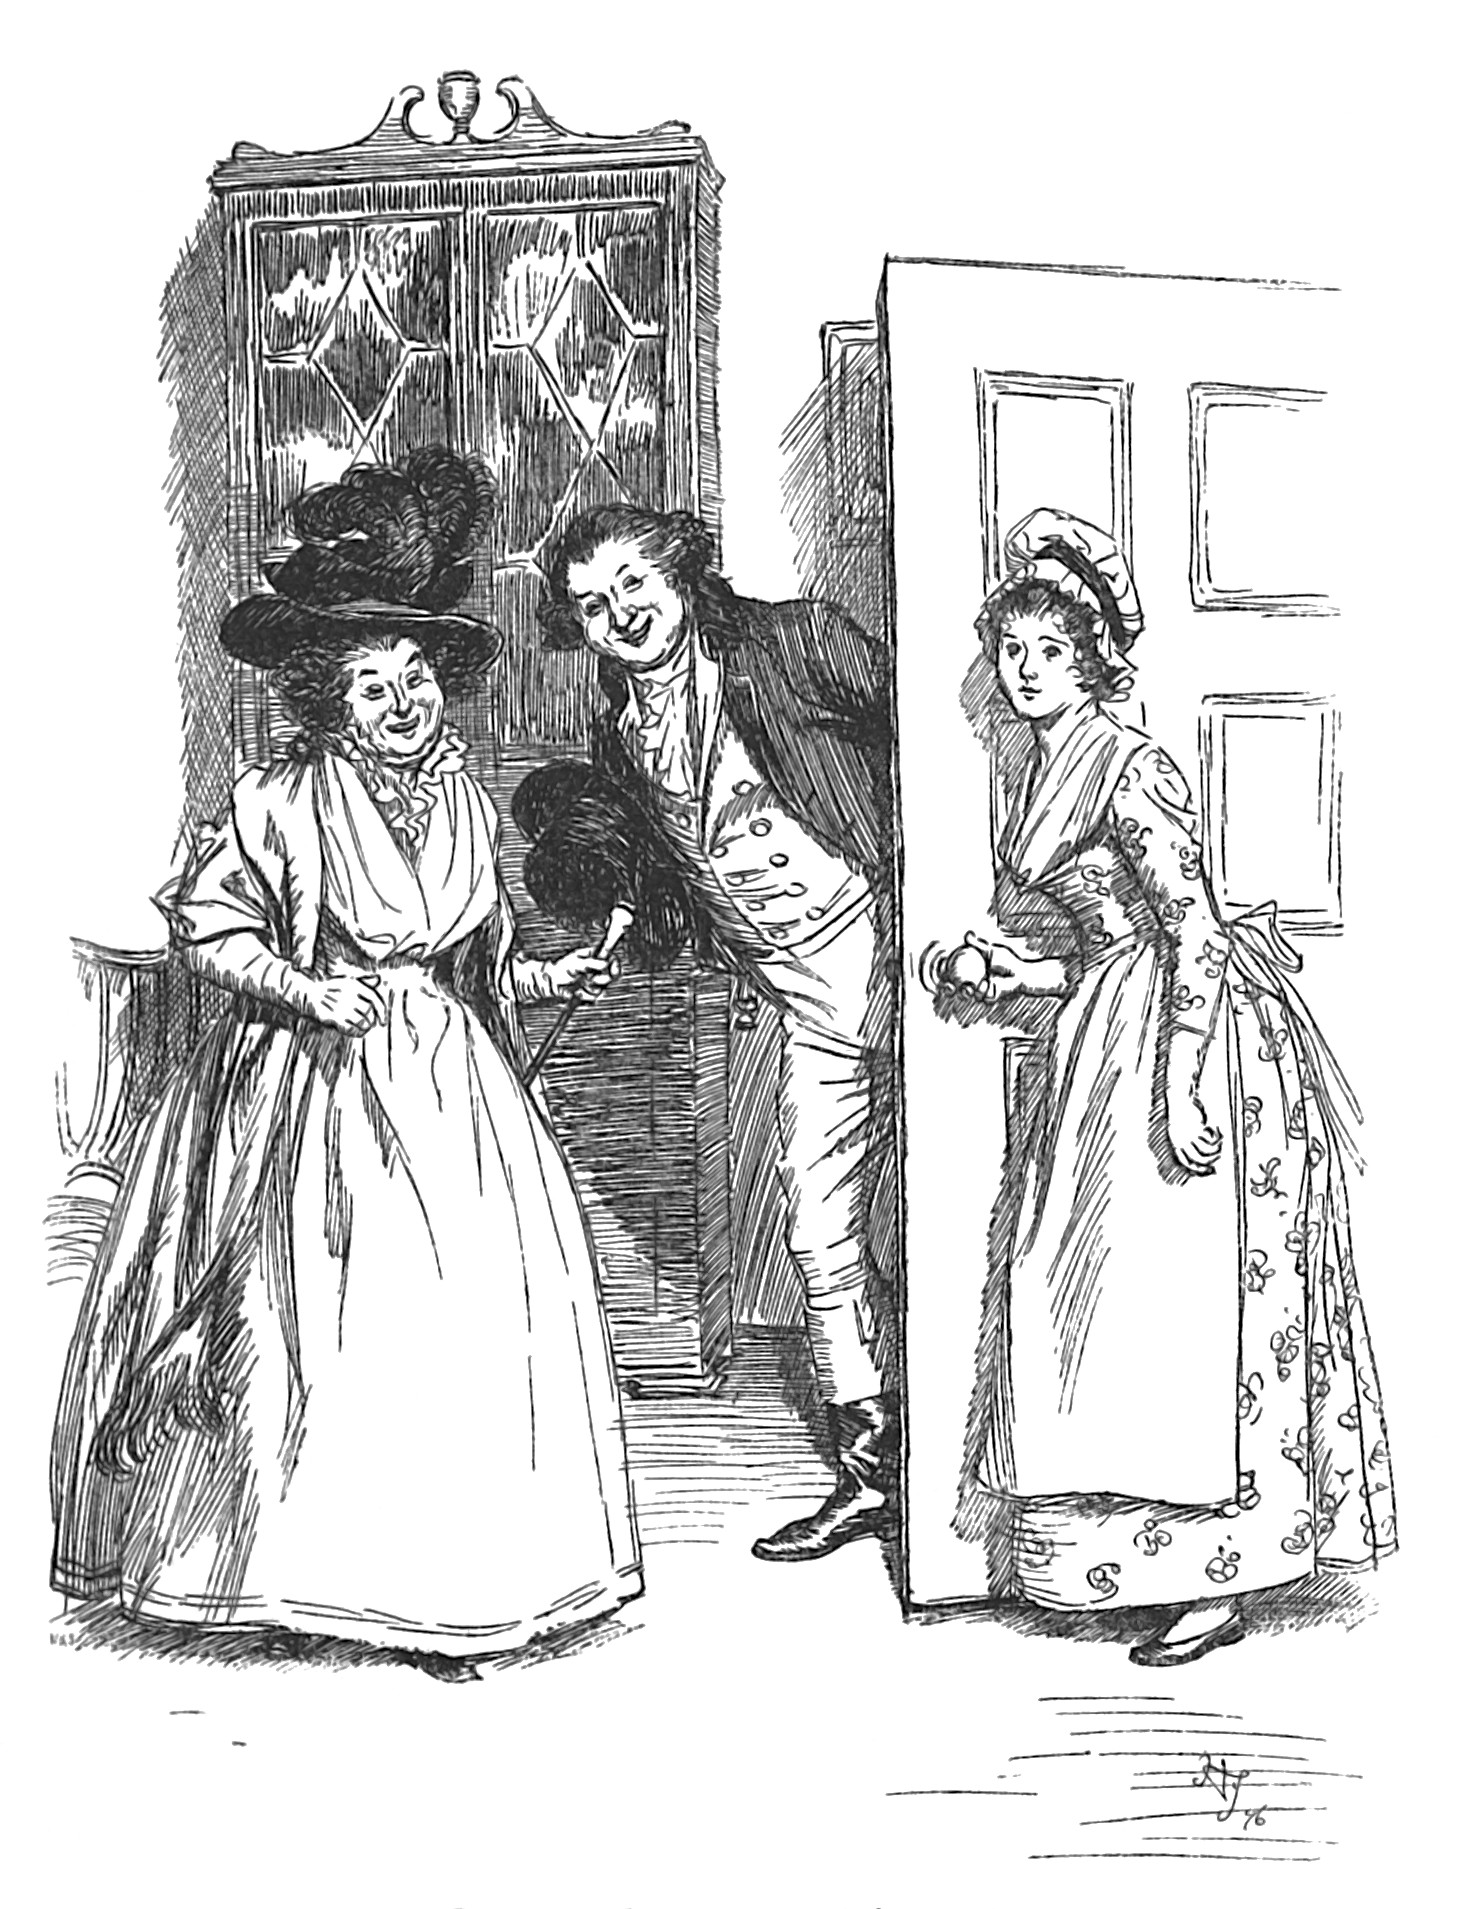
\includegraphics[width=\linewidth]{18guest}
\caption{Came to take a survey of the guest}
\end{figure}

Sir John never came to the Dashwoods without either inviting them to dine at the park the next day, or to drink tea with them that evening. On the present occasion, for the better entertainment of their visitor, towards whose amusement he felt himself bound to contribute, he wished to engage them for both.

»You \textit{must} drink tea with us to night,« said he, »for we shall be quite alone—and tomorrow you must absolutely dine with us, for we shall be a large party.«

Mrs Jennings enforced the necessity. »And who knows but \textit{you} may raise a dance,« said she. »And that will tempt you, Miss Marianne.«

»A dance!« cried Marianne. »Impossible! Who is to dance?«

»Who! why yourselves, and the Careys, and Whitakers to be sure.—What! you thought nobody could dance because a certain person that shall be nameless is gone!«

»I wish with all my soul,« cried Sir John, »that Willoughby were among us again.«

This, and Marianne’s blushing, gave new suspicions to Edward. »And who is Willoughby?« said he, in a low voice, to Miss Dashwood, by whom he was sitting.

She gave him a brief reply. Marianne’s countenance was more communicative. Edward saw enough to comprehend, not only the meaning of others, but such of Marianne’s expressions as had puzzled him before; and when their visitors left them, he went immediately round her, and said, in a whisper, »I have been guessing. Shall I tell you my guess?«

»What do you mean?«

»Shall I tell you?«

»Certainly.«

»Well then; I guess that Mr Willoughby hunts.«

Marianne was surprised and confused, yet she could not help smiling at the quiet archness of his manner, and after a moment’s silence, said,

»Oh, Edward! How can you?—But the time will come I hope...I am sure you will like him.«

»I do not doubt it,« replied he, rather astonished at her earnestness and warmth; for had he not imagined it to be a joke for the good of her acquaintance in general, founded only on a something or a nothing between Mr Willoughby and herself, he would not have ventured to mention it.
%!TeX root=../emmatop.tex
\chapter[Chapter \thechapter]{}
\lettrine[lraise=0.3]{E}{mma} and Harriet had been walking together one morning, and, in Emma's opinion, had been talking enough of Mr Elton for that day. She could not think that Harriet's solace or her own sins required more; and she was therefore industriously getting rid of the subject as they returned;—but it burst out again when she thought she had succeeded, and after speaking some time of what the poor must suffer in winter, and receiving no other answer than a very plaintive—<Mr Elton is so good to the poor!> she found something else must be done.

They were just approaching the house where lived Mrs and Miss Bates. She determined to call upon them and seek safety in numbers. There was always sufficient reason for such an attention; Mrs and Miss Bates loved to be called on, and she knew she was considered by the very few who presumed ever to see imperfection in her, as rather negligent in that respect, and as not contributing what she ought to the stock of their scanty comforts.

She had had many a hint from Mr Knightley and some from her own heart, as to her deficiency—but none were equal to counteract the persuasion of its being very disagreeable,—a waste of time—tiresome women—and all the horror of being in danger of falling in with the second-rate and third-rate of Highbury, who were calling on them for ever, and therefore she seldom went near them. But now she made the sudden resolution of not passing their door without going in—observing, as she proposed it to Harriet, that, as well as she could calculate, they were just now quite safe from any letter from Jane Fairfax.

The house belonged to people in business. Mrs and Miss Bates occupied the drawing-room floor; and there, in the very moderate-sized apartment, which was every thing to them, the visitors were most cordially and even gratefully welcomed; the quiet neat old lady, who with her knitting was seated in the warmest corner, wanting even to give up her place to Miss Woodhouse, and her more active, talking daughter, almost ready to overpower them with care and kindness, thanks for their visit, solicitude for their shoes, anxious inquiries after Mr Woodhouse's health, cheerful communications about her mother's, and sweet-cake from the beaufet—<Mrs Cole had just been there, just called in for ten minutes, and had been so good as to sit an hour with them, and she had taken a piece of cake and been so kind as to say she liked it very much; and, therefore, she hoped Miss Woodhouse and Miss Smith would do them the favour to eat a piece too.>

The mention of the Coles was sure to be followed by that of Mr Elton. There was intimacy between them, and Mr Cole had heard from Mr Elton since his going away. Emma knew what was coming; they must have the letter over again, and settle how long he had been gone, and how much he was engaged in company, and what a favourite he was wherever he went, and how full the Master of the Ceremonies' ball had been; and she went through it very well, with all the interest and all the commendation that could be requisite, and always putting forward to prevent Harriet's being obliged to say a word.

This she had been prepared for when she entered the house; but meant, having once talked him handsomely over, to be no farther incommoded by any troublesome topic, and to wander at large amongst all the Mistresses and Misses of Highbury, and their card-parties. She had not been prepared to have Jane Fairfax succeed Mr Elton; but he was actually hurried off by Miss Bates, she jumped away from him at last abruptly to the Coles, to usher in a letter from her niece.

<Oh! yes—Mr Elton, I understand—certainly as to dancing—Mrs Cole was telling me that dancing at the rooms at Bath was—Mrs Cole was so kind as to sit some time with us, talking of Jane; for as soon as she came in, she began inquiring after her, Jane is so very great a favourite there. Whenever she is with us, Mrs Cole does not know how to shew her kindness enough; and I must say that Jane deserves it as much as any body can. And so she began inquiring after her directly, saying, <I know you cannot have heard from Jane lately, because it is not her time for writing;> and when I immediately said, <But indeed we have, we had a letter this very morning,> I do not know that I ever saw any body more surprized. <Have you, upon your honour?> said she; <well, that is quite unexpected. Do let me hear what she says.>>

Emma's politeness was at hand directly, to say, with smiling interest—

<Have you heard from Miss Fairfax so lately? I am extremely happy. I hope she is well?>

\begin{figure}[tbph]
\centering
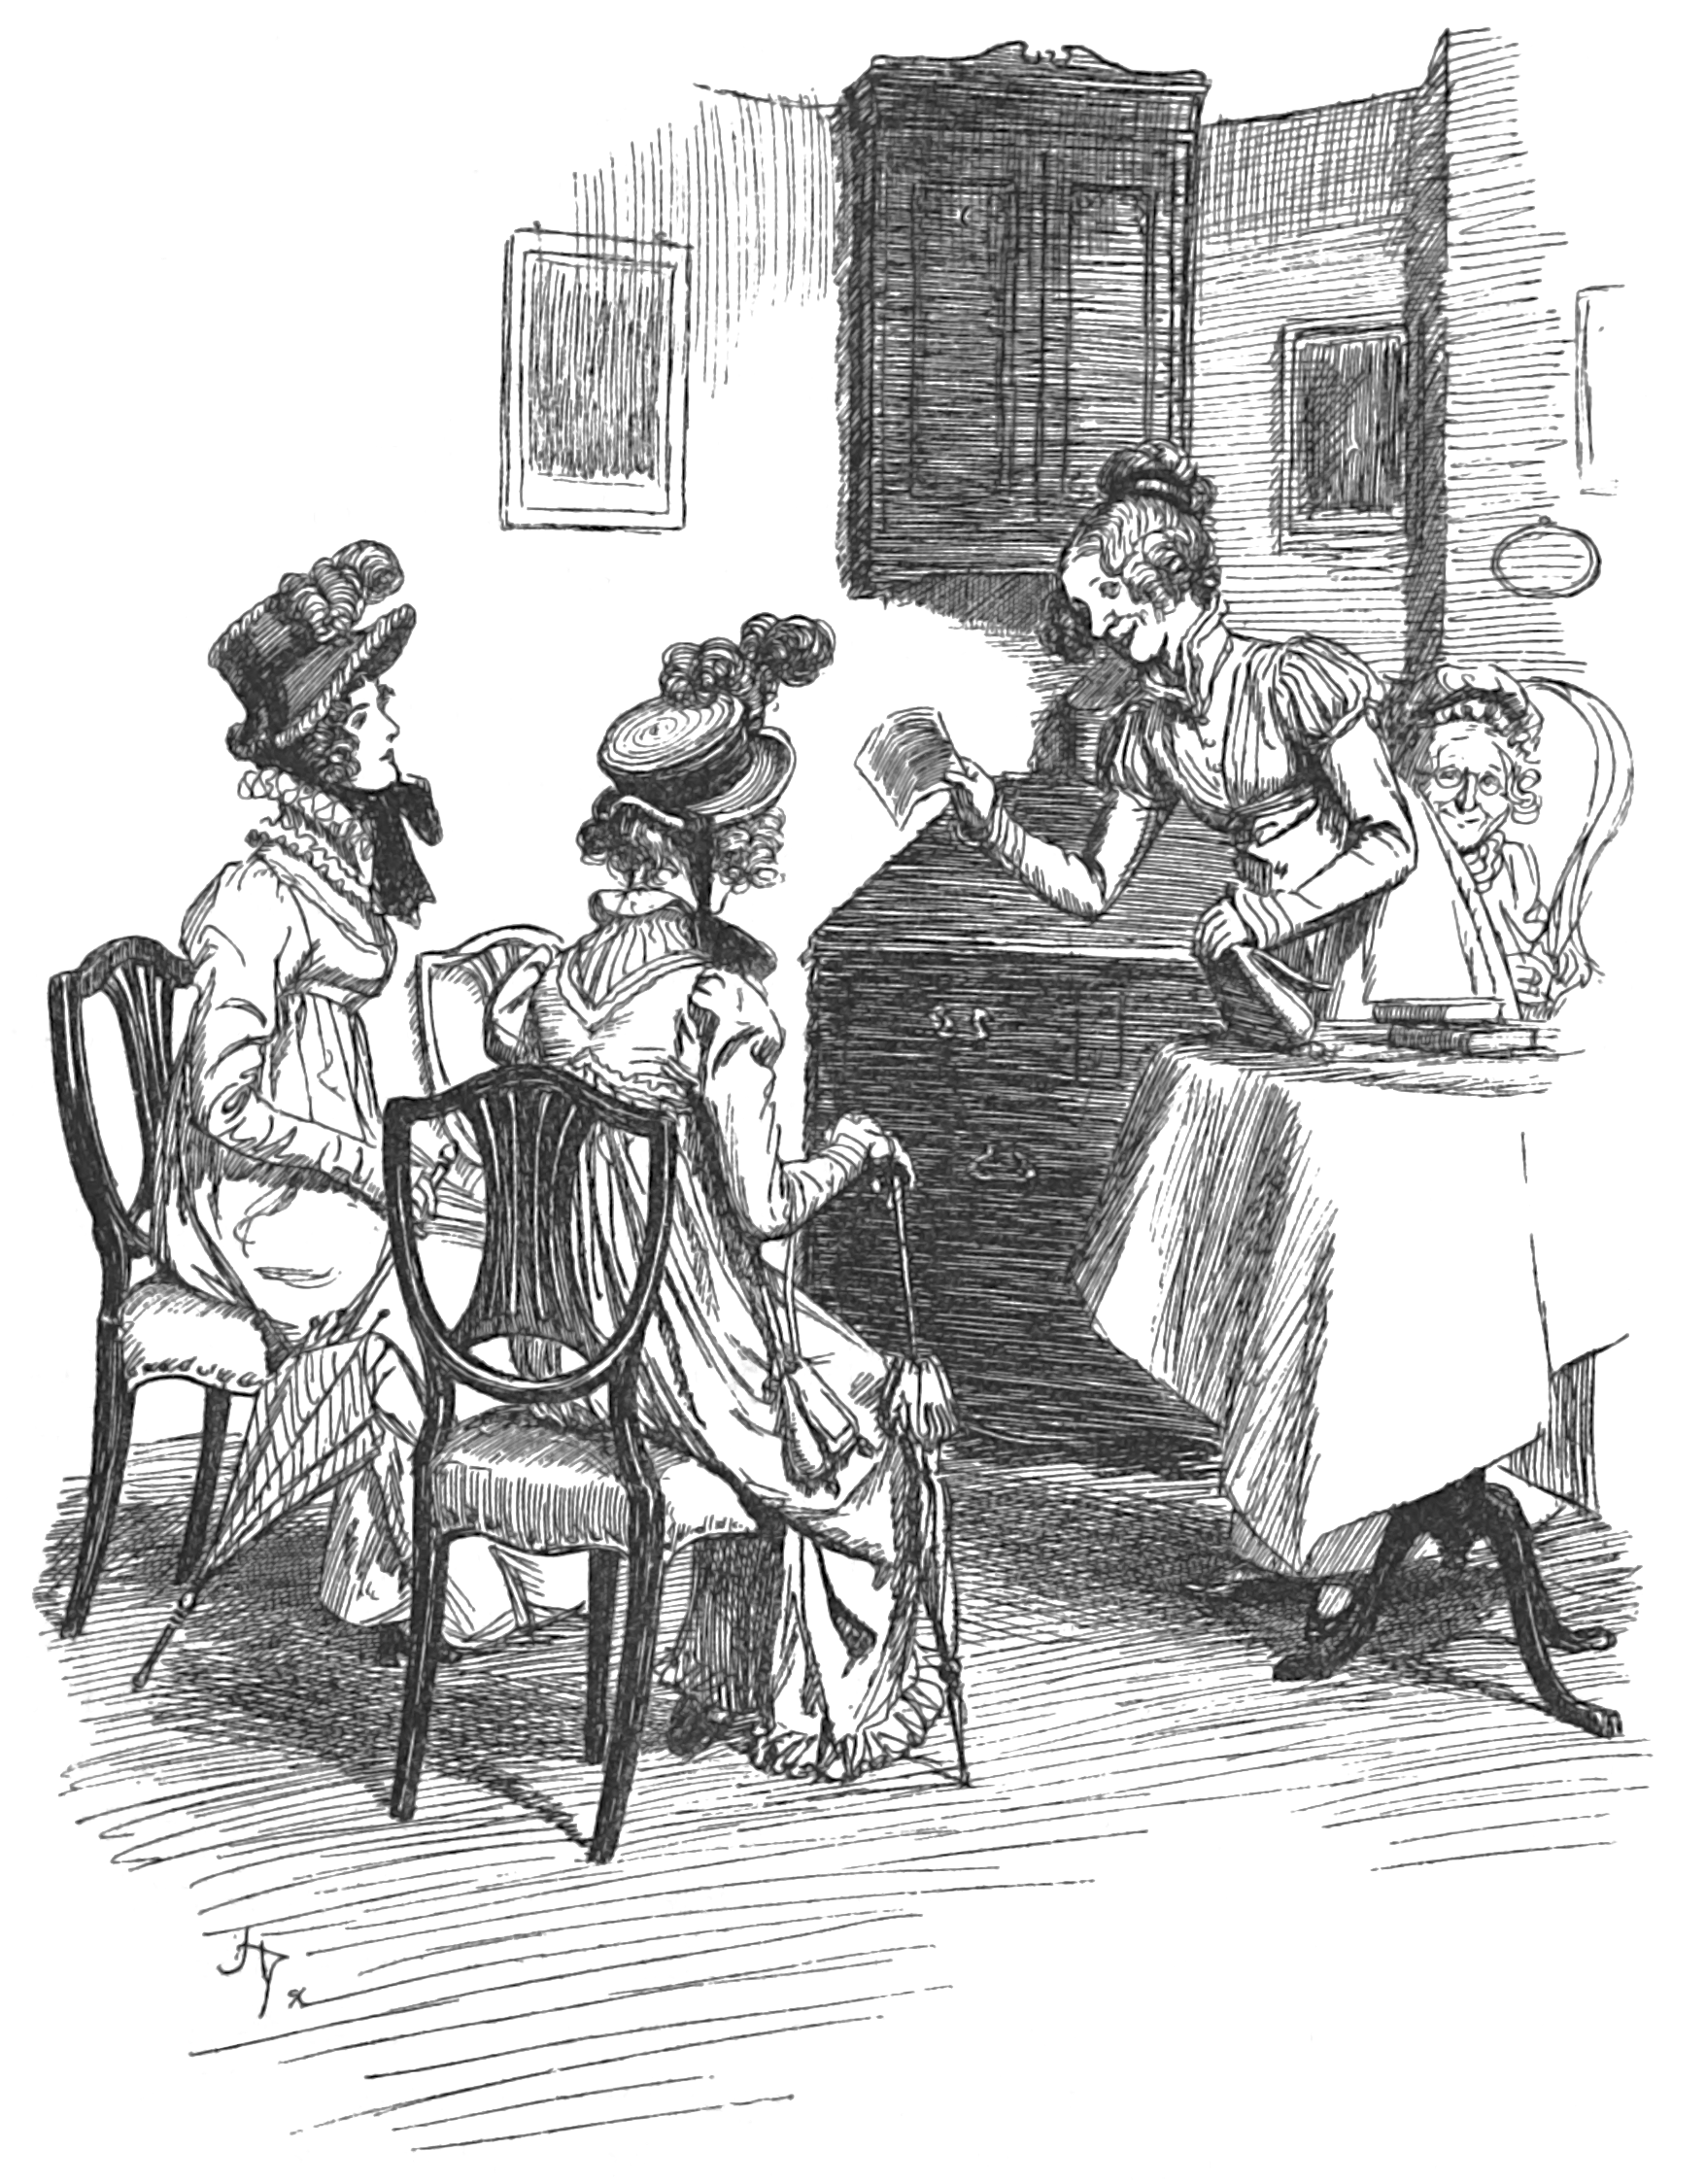
\includegraphics[width=\linewidth]{19hereitis}
\caption{<Oh! here it is.>}
\end{figure}

<Thank you. You are so kind!> replied the happily deceived aunt, while eagerly hunting for the letter.—<Oh! here it is. I was sure it could not be far off; but I had put my huswife upon it, you see, without being aware, and so it was quite hid, but I had it in my hand so very lately that I was almost sure it must be on the table. I was reading it to Mrs Cole, and since she went away, I was reading it again to my mother, for it is such a pleasure to her—a letter from Jane—that she can never hear it often enough; so I knew it could not be far off, and here it is, only just under my huswife—and since you are so kind as to wish to hear what she says;—but, first of all, I really must, in justice to Jane, apologise for her writing so short a letter—only two pages you see—hardly two—and in general she fills the whole paper and crosses half. My mother often wonders that I can make it out so well. She often says, when the letter is first opened, <Well, Hetty, now I think you will be put to it to make out all that checker-work>—don't you, ma'am?—And then I tell her, I am sure she would contrive to make it out herself, if she had nobody to do it for her—every word of it—I am sure she would pore over it till she had made out every word. And, indeed, though my mother's eyes are not so good as they were, she can see amazingly well still, thank God! with the help of spectacles. It is such a blessing! My mother's are really very good indeed. Jane often says, when she is here, <I am sure, grandmama, you must have had very strong eyes to see as you do—and so much fine work as you have done too!—I only wish my eyes may last me as well.>>

All this spoken extremely fast obliged Miss Bates to stop for breath; and Emma said something very civil about the excellence of Miss Fairfax's handwriting.

<You are extremely kind,> replied Miss Bates, highly gratified; <you who are such a judge, and write so beautifully yourself. I am sure there is nobody's praise that could give us so much pleasure as Miss Woodhouse's. My mother does not hear; she is a little deaf you know. Ma'am,> addressing her, <do you hear what Miss Woodhouse is so obliging to say about Jane's handwriting?>

And Emma had the advantage of hearing her own silly compliment repeated twice over before the good old lady could comprehend it. She was pondering, in the meanwhile, upon the possibility, without seeming very rude, of making her escape from Jane Fairfax's letter, and had almost resolved on hurrying away directly under some slight excuse, when Miss Bates turned to her again and seized her attention.

<My mother's deafness is very trifling you see—just nothing at all. By only raising my voice, and saying any thing two or three times over, she is sure to hear; but then she is used to my voice. But it is very remarkable that she should always hear Jane better than she does me. Jane speaks so distinct! However, she will not find her grandmama at all deafer than she was two years ago; which is saying a great deal at my mother's time of life—and it really is full two years, you know, since she was here. We never were so long without seeing her before, and as I was telling Mrs Cole, we shall hardly know how to make enough of her now.>

<Are you expecting Miss Fairfax here soon?>

<Oh yes; next week.>

<Indeed!—that must be a very great pleasure.>

<Thank you. You are very kind. Yes, next week. Every body is so surprized; and every body says the same obliging things. I am sure she will be as happy to see her friends at Highbury, as they can be to see her. Yes, Friday or Saturday; she cannot say which, because Colonel Campbell will be wanting the carriage himself one of those days. So very good of them to send her the whole way! But they always do, you know. Oh yes, Friday or Saturday next. That is what she writes about. That is the reason of her writing out of rule, as we call it; for, in the common course, we should not have heard from her before next Tuesday or Wednesday.>

<Yes, so I imagined. I was afraid there could be little chance of my hearing any thing of Miss Fairfax to-day.>

<So obliging of you! No, we should not have heard, if it had not been for this particular circumstance, of her being to come here so soon. My mother is so delighted!—for she is to be three months with us at least. Three months, she says so, positively, as I am going to have the pleasure of reading to you. The case is, you see, that the Campbells are going to Ireland. Mrs Dixon has persuaded her father and mother to come over and see her directly. They had not intended to go over till the summer, but she is so impatient to see them again—for till she married, last October, she was never away from them so much as a week, which must make it very strange to be in different kingdoms, I was going to say, but however different countries, and so she wrote a very urgent letter to her mother—or her father, I declare I do not know which it was, but we shall see presently in Jane's letter—wrote in Mr Dixon's name as well as her own, to press their coming over directly, and they would give them the meeting in Dublin, and take them back to their country seat, Baly-craig, a beautiful place, I fancy. Jane has heard a great deal of its beauty; from Mr Dixon, I mean—I do not know that she ever heard about it from any body else; but it was very natural, you know, that he should like to speak of his own place while he was paying his addresses—and as Jane used to be very often walking out with them—for Colonel and Mrs Campbell were very particular about their daughter's not walking out often with only Mr Dixon, for which I do not at all blame them; of course she heard every thing he might be telling Miss Campbell about his own home in Ireland; and I think she wrote us word that he had shewn them some drawings of the place, views that he had taken himself. He is a most amiable, charming young man, I believe. Jane was quite longing to go to Ireland, from his account of things.>

At this moment, an ingenious and animating suspicion entering Emma's brain with regard to Jane Fairfax, this charming Mr Dixon, and the not going to Ireland, she said, with the insidious design of farther discovery,

<You must feel it very fortunate that Miss Fairfax should be allowed to come to you at such a time. Considering the very particular friendship between her and Mrs Dixon, you could hardly have expected her to be excused from accompanying Colonel and Mrs Campbell.>

<Very true, very true, indeed. The very thing that we have always been rather afraid of; for we should not have liked to have her at such a distance from us, for months together—not able to come if any thing was to happen. But you see, every thing turns out for the best. They want her (Mr and Mrs Dixon) excessively to come over with Colonel and Mrs Campbell; quite depend upon it; nothing can be more kind or pressing than their joint invitation, Jane says, as you will hear presently; Mr Dixon does not seem in the least backward in any attention. He is a most charming young man. Ever since the service he rendered Jane at Weymouth, when they were out in that party on the water, and she, by the sudden whirling round of something or other among the sails, would have been dashed into the sea at once, and actually was all but gone, if he had not, with the greatest presence of mind, caught hold of her habit— (I can never think of it without trembling!)—But ever since we had the history of that day, I have been so fond of Mr Dixon!>

<But, in spite of all her friends' urgency, and her own wish of seeing Ireland, Miss Fairfax prefers devoting the time to you and Mrs Bates?>

<Yes—entirely her own doing, entirely her own choice; and Colonel and Mrs Campbell think she does quite right, just what they should recommend; and indeed they particularly wish her to try her native air, as she has not been quite so well as usual lately.>

<I am concerned to hear of it. I think they judge wisely. But Mrs Dixon must be very much disappointed. Mrs Dixon, I understand, has no remarkable degree of personal beauty; is not, by any means, to be compared with Miss Fairfax.>

<Oh! no. You are very obliging to say such things—but certainly not. There is no comparison between them. Miss Campbell always was absolutely plain—but extremely elegant and amiable.>

<Yes, that of course.>

<Jane caught a bad cold, poor thing! so long ago as the 7th of November, (as I am going to read to you,) and has never been well since. A long time, is not it, for a cold to hang upon her? She never mentioned it before, because she would not alarm us. Just like her! so considerate!—But however, she is so far from well, that her kind friends the Campbells think she had better come home, and try an air that always agrees with her; and they have no doubt that three or four months at Highbury will entirely cure her—and it is certainly a great deal better that she should come here, than go to Ireland, if she is unwell. Nobody could nurse her, as we should do.>

<It appears to me the most desirable arrangement in the world.>

<And so she is to come to us next Friday or Saturday, and the Campbells leave town in their way to Holyhead the Monday following—as you will find from Jane's letter. So sudden!—You may guess, dear Miss Woodhouse, what a flurry it has thrown me in! If it was not for the drawback of her illness—but I am afraid we must expect to see her grown thin, and looking very poorly. I must tell you what an unlucky thing happened to me, as to that. I always make a point of reading Jane's letters through to myself first, before I read them aloud to my mother, you know, for fear of there being any thing in them to distress her. Jane desired me to do it, so I always do: and so I began to-day with my usual caution; but no sooner did I come to the mention of her being unwell, than I burst out, quite frightened, with <Bless me! poor Jane is ill!>—which my mother, being on the watch, heard distinctly, and was sadly alarmed at. However, when I read on, I found it was not near so bad as I had fancied at first; and I make so light of it now to her, that she does not think much about it. But I cannot imagine how I could be so off my guard. If Jane does not get well soon, we will call in Mr Perry. The expense shall not be thought of; and though he is so liberal, and so fond of Jane that I dare say he would not mean to charge any thing for attendance, we could not suffer it to be so, you know. He has a wife and family to maintain, and is not to be giving away his time. Well, now I have just given you a hint of what Jane writes about, we will turn to her letter, and I am sure she tells her own story a great deal better than I can tell it for her.>

<I am afraid we must be running away,> said Emma, glancing at Harriet, and beginning to rise—<My father will be expecting us. I had no intention, I thought I had no power of staying more than five minutes, when I first entered the house. I merely called, because I would not pass the door without inquiring after Mrs Bates; but I have been so pleasantly detained! Now, however, we must wish you and Mrs Bates good morning.>

And not all that could be urged to detain her succeeded. She regained the street—happy in this, that though much had been forced on her against her will, though she had in fact heard the whole substance of Jane Fairfax's letter, she had been able to escape the letter itself.
%!TeX root=../pridetop.tex
\chapter[Chapter \thechapter]{}
\begin{figure}[t!]
\centering
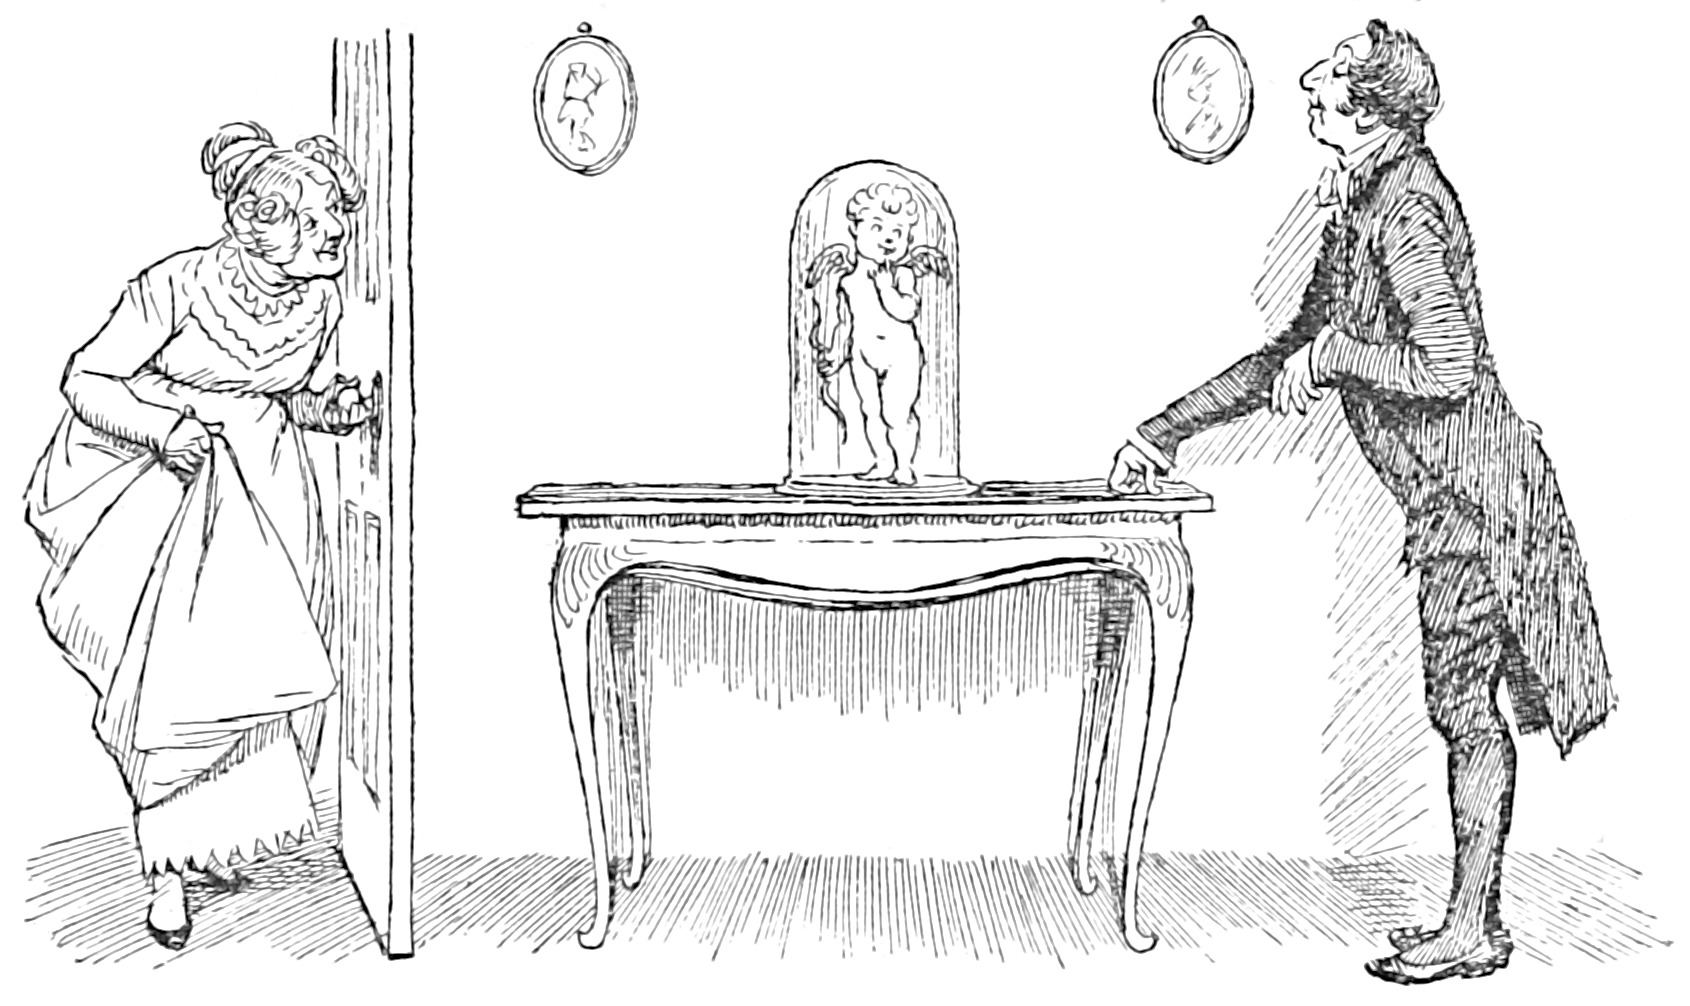
\includegraphics[width=\linewidth]{20top}
\captionlistentry{Headpiece to Chapter \thechapter}
\end{figure}

\lettrine[lines=6,image=true]{initials/chap20m}{r}  Collins was not left long to the silent contemplation of his successful love; for Mrs Bennet, having dawdled about in the vestibule to watch for the end of the conference, no sooner saw Elizabeth open the door and with quick step pass her towards the staircase, than she entered the breakfast-room, and congratulated both him and herself in warm terms on the happy prospect of their nearer connection. Mr Collins received and returned these felicitations with equal pleasure, and then proceeded to relate the particulars of their interview, with the result of which he trusted he had every reason to be satisfied, since the refusal which his cousin had steadfastly given him would naturally flow from her bashful modesty and the genuine delicacy of her character.

This information, however, startled Mrs Bennet: she would have been glad to be equally satisfied that her daughter had meant to encourage him by protesting against his proposals, but she dared not believe it, and could not help saying so.

<But depend upon it, Mr Collins,> she added, <that Lizzy shall be brought to reason. I will speak to her about it myself directly. She is a very headstrong, foolish girl, and does not know her own interest; but I will \textit{make} her know it.>

<Pardon me for interrupting you, madam,> cried Mr Collins; <but if she is really headstrong and foolish, I know not whether she would altogether be a very desirable wife to a man in my situation, who naturally looks for happiness in the marriage state. If, therefore, she actually persists in rejecting my suit, perhaps it were better not to force her into accepting me, because, if liable to such defects of temper, she could not contribute much to my felicity.>

<Sir, you quite misunderstand me,> said Mrs Bennet, alarmed. <Lizzy is only headstrong in such matters as these. In everything else she is as good-natured a girl as ever lived. I will go directly to Mr Bennet, and we shall very soon settle it with her, I am sure.>

She would not give him time to reply, but hurrying instantly to her husband, called out, as she entered the library,—

<Oh, Mr Bennet, you are wanted immediately; we are all in an uproar. You must come and make Lizzy marry Mr Collins, for she vows she will not have him; and if you do not make haste he will change his mind and not have \textit{her}.>

Mr Bennet raised his eyes from his book as she entered, and fixed them on her face with a calm unconcern, which was not in the least altered by her communication.

<I have not the pleasure of understanding you,> said he, when she had finished her speech. <Of what are you talking?>

<Of Mr Collins and Lizzy. Lizzy declares she will not have Mr Collins, and Mr Collins begins to say that he will not have Lizzy.>

<And what am I to do on the occasion? It seems a hopeless business.>

<Speak to Lizzy about it yourself. Tell her that you insist upon her marrying him.>

<Let her be called down. She shall hear my opinion.>

Mrs Bennet rang the bell, and Miss Elizabeth was summoned to the library.

<Come here, child,> cried her father as she appeared. <I have sent for you on an affair of importance. I understand that Mr Collins has made you an offer of marriage. Is it true?>

Elizabeth replied that it was.

<Very well—and this offer of marriage you have refused?>

<I have, sir.>

<Very well. We now come to the point. Your mother insists upon your accepting it. Is it not so, Mrs Bennet?>

<Yes, or I will never see her again.>

<An unhappy alternative is before you, Elizabeth. From this day you must be a stranger to one of your parents. Your mother will never see you again if you do \textit{not} marry Mr Collins, and I will never see you again if you \textit{do}.>

Elizabeth could not but smile at such a conclusion of such a beginning; but Mrs Bennet, who had persuaded herself that her husband regarded the affair as she wished, was excessively disappointed.

<What do you mean, Mr Bennet, by talking in this way? You promised me to \textit{insist} upon her marrying him.>

<My dear,> replied her husband, <I have two small favours to request. First, that you will allow me the free use of my understanding on the present occasion; and, secondly, of my room. I shall be glad to have the library to myself as soon as may be.>

Not yet, however, in spite of her disappointment in her husband, did Mrs Bennet give up the point. She talked to Elizabeth again and again; coaxed and threatened her by turns. She endeavoured to secure Jane in her interest, but Jane, with all possible mildness, declined interfering; and Elizabeth, sometimes with real earnestness, and sometimes with playful gaiety, replied to her attacks. Though her manner varied, however, her determination never did.

Mr Collins, meanwhile, was meditating in solitude on what had passed. He thought too well of himself to comprehend on what motive his cousin could refuse him; and though his pride was hurt, he suffered in no other way. His regard for her was quite imaginary; and the possibility of her deserving her mother's reproach prevented his feeling any regret.

While the family were in this confusion, Charlotte Lucas came to spend the day with them. She was met in the vestibule by Lydia, who, flying to her, cried in a half whisper, <I am glad you are come, for there is such fun here! What do you think has happened this morning? Mr Collins has made an offer to Lizzy, and she will not have him.>

Charlotte had hardly time to answer before they were joined by Kitty, who came to tell the same news; and no sooner had they entered the breakfast-room, where Mrs Bennet was alone, than she likewise began on the subject, calling on Miss Lucas for her compassion, and entreating her to persuade her friend Lizzy to comply with the wishes of her family. <Pray do, my dear Miss Lucas,> she added, in a melancholy tone; <for nobody is on my side, nobody takes part with me; I am cruelly used, nobody feels for my poor nerves.>

\begin{figure}[tbh]
\centering
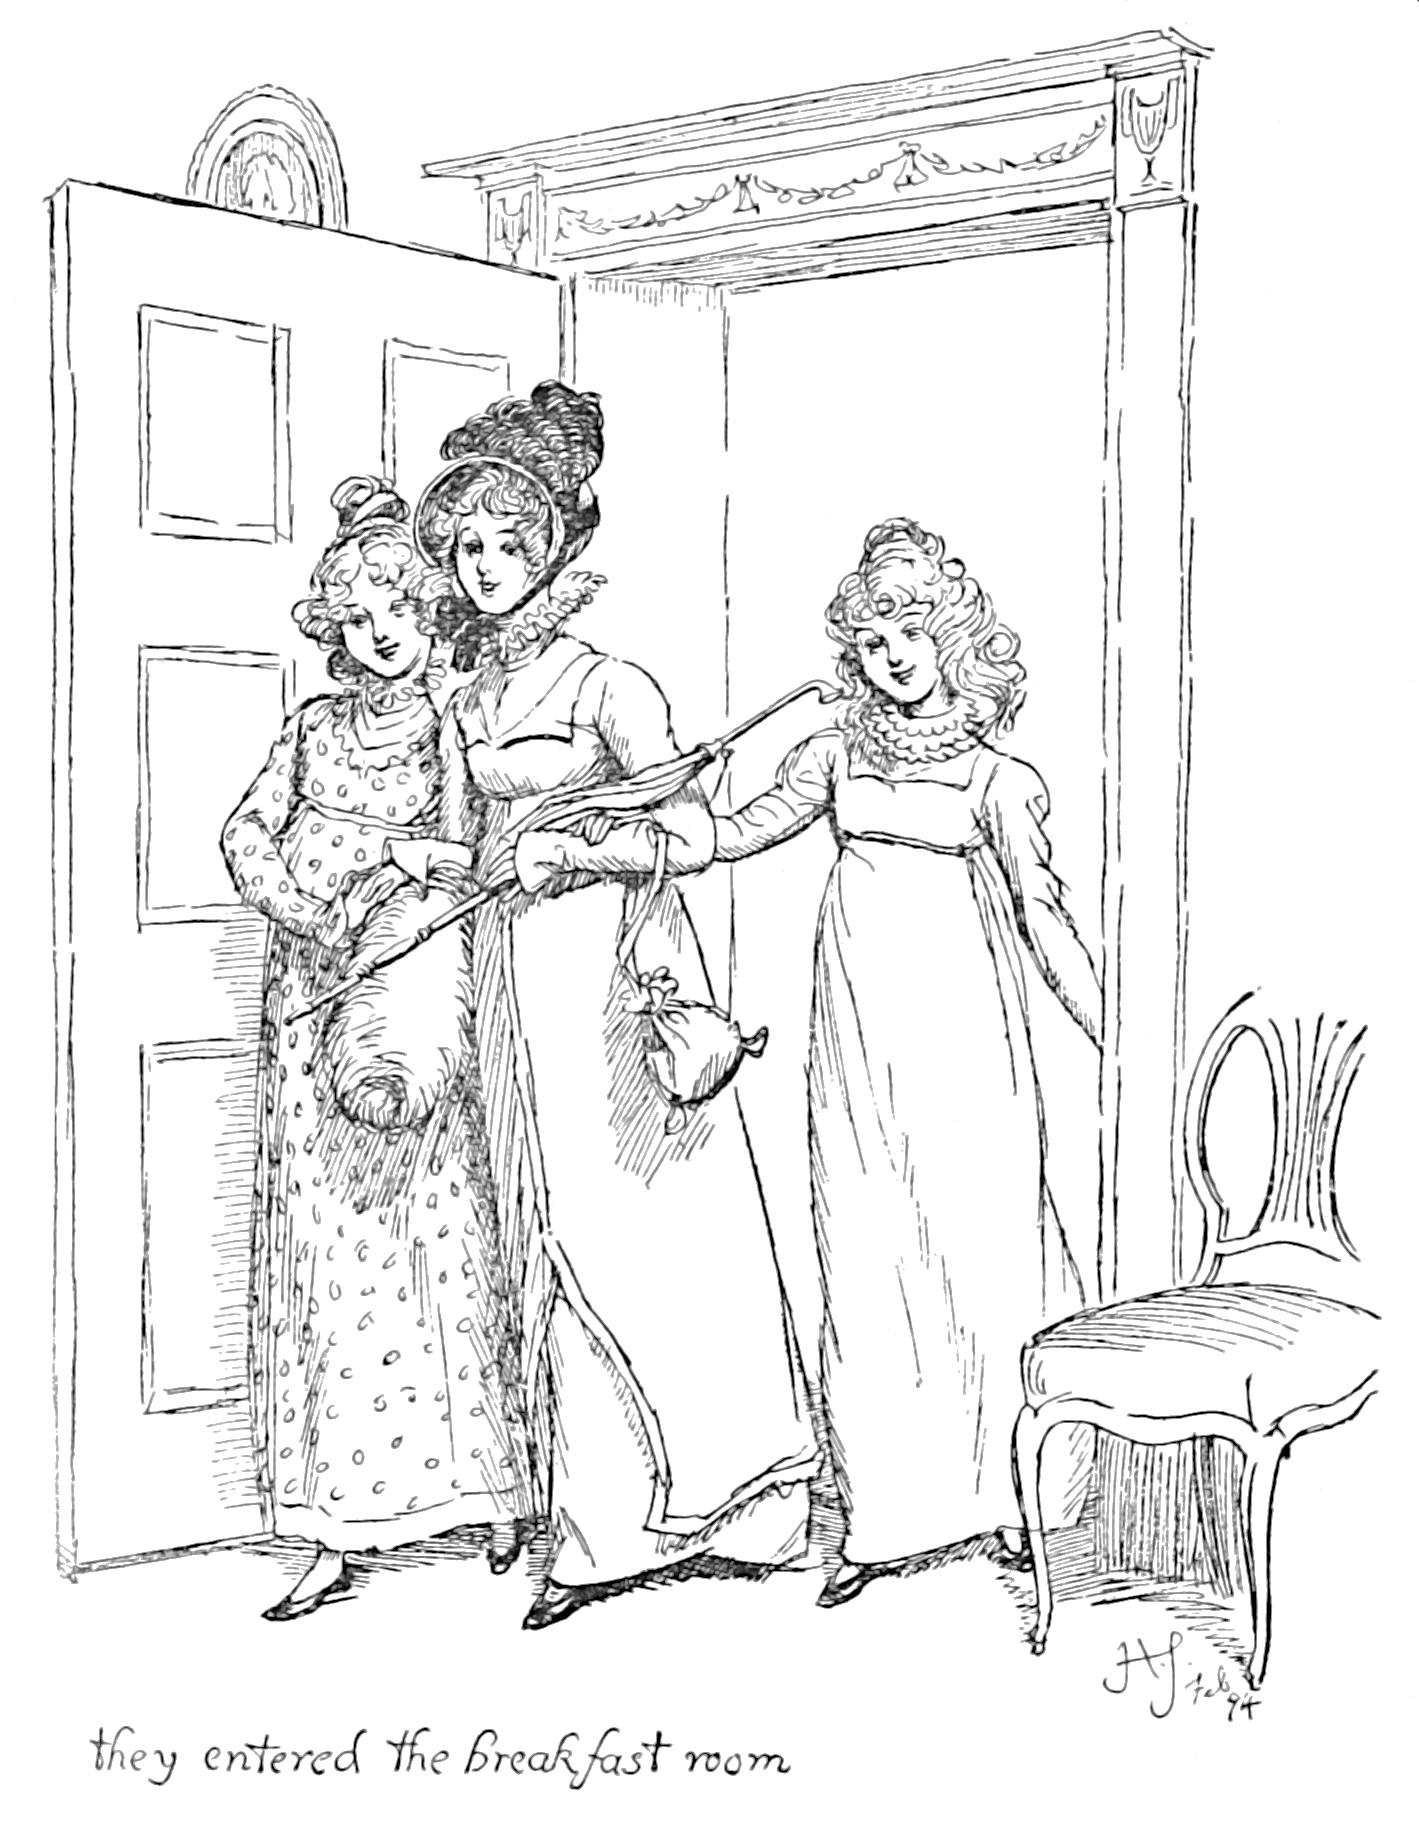
\includegraphics[width=.8\linewidth]{20breakfast}
\captionlistentry{They entered the breakfast room}
\end{figure}

Charlotte's reply was spared by the entrance of Jane and Elizabeth.

<Ay, there she comes,> continued Mrs Bennet, <looking as unconcerned as may be, and caring no more for us than if we were at York, provided she can have her own way. But I tell you what, Miss Lizzy, if you take it into your head to go on refusing every offer of marriage in this way, you will never get a husband at all—and I am sure I do not know who is to maintain you when your father is dead. \textit{I} shall not be able to keep you—and so I warn you. I have done with you from this very day. I told you in the library, you know, that I should never speak to you again, and you will find me as good as my word. I have no pleasure in talking to undutiful children. Not that I have much pleasure, indeed, in talking to anybody. People who suffer as I do from nervous complaints can have no great inclination for talking. Nobody can tell what I suffer! But it is always so. Those who do not complain are never pitied.>

Her daughters listened in silence to this effusion, sensible that any attempt to reason with or soothe her would only increase the irritation. She talked on, therefore, without interruption from any of them till they were joined by Mr Collins, who entered with an air more stately than usual, and on perceiving whom, she said to the girls,—

<Now, I do insist upon it, that you, all of you, hold your tongues, and let Mr Collins and me have a little conversation together.>

Elizabeth passed quietly out of the room, Jane and Kitty followed, but Lydia stood her ground, determined to hear all she could; and Charlotte, detained first by the civility of Mr Collins, whose inquiries after herself and all her family were very minute, and then by a little curiosity, satisfied herself with walking to the window and pretending not to hear. In a doleful voice Mrs Bennet thus began the projected conversation:—

<Oh, Mr Collins!>

<My dear madam,> replied he, <let us be for ever silent on this point. Far be it from me,> he presently continued, in a voice that marked his displeasure, <to resent the behaviour of your daughter. Resignation to inevitable evils is the duty of us all: the peculiar duty of a young man who has been so fortunate as I have been, in early preferment; and, I trust, I am resigned. Perhaps not the less so from feeling a doubt of my positive happiness had my fair cousin honoured me with her hand; for I have often observed, that resignation is never so perfect as when the blessing denied begins to lose somewhat of its value in our estimation. You will not, I hope, consider me as showing any disrespect to your family, my dear madam, by thus withdrawing my pretensions to your daughter's favour, without having paid yourself and Mr Bennet the compliment of requesting you to interpose your authority in my behalf. My conduct may, I fear, be objectionable in having accepted my dismission from your daughter's lips instead of your own; but we are all liable to error. I have certainly meant well through the whole affair. My object has been to secure an amiable companion for myself, with due consideration for the advantage of all your family; and if my \textit{manner} has been at all reprehensible, I here beg leave to apologize.>


\chapter[Chapter \thechapter]{} 

 \lettrine[lraise=0.3]{S}{ir} Thomas's return made a striking change in the ways of the family, independent of Lovers' Vows. Under his government, Mansfield was an altered place. Some members of their society sent away, and the spirits of many others saddened—it was all sameness and gloom compared with the past—a sombre family party rarely enlivened. There was little intercourse with the Parsonage. Sir~Thomas, drawing back from intimacies in general, was particularly disinclined, at this time, for any engagements but in one quarter. The Rushworths were the only addition to his own domestic circle which he could solicit.

Edmund did not wonder that such should be his father's feelings, nor could he regret anything but the exclusion of the Grants. <But they,> he observed to Fanny, <have a claim. They seem to belong to us; they seem to be part of ourselves. I could wish my father were more sensible of their very great attention to my mother and sisters while he was away. I am afraid they may feel themselves neglected. But the truth is, that my father hardly knows them. They had not been here a twelvemonth when he left England. If he knew them better, he would value their society as it deserves; for they are in fact exactly the sort of people he would like. We are sometimes a little in want of animation among ourselves: my sisters seem out of spirits, and Tom is certainly not at his ease. Dr~and Mrs~Grant would enliven us, and make our evenings pass away with more enjoyment even to my father.>

<Do you think so?> said Fanny: <in my opinion, my uncle would not like \textit{any}  addition. I think he values the very quietness you speak of, and that the repose of his own family circle is all he wants. And it does not appear to me that we are more serious than we used to be—I mean before my uncle went abroad. As well as I can recollect, it was always much the same. There was never much laughing in his presence; or, if there is any difference, it is not more, I think, than such an absence has a tendency to produce at first. There must be a sort of shyness; but I cannot recollect that our evenings formerly were ever merry, except when my uncle was in town. No young people's are, I suppose, when those they look up to are at home>.

<I believe you are right, Fanny,> was his reply, after a short consideration. <I believe our evenings are rather returned to what they were, than assuming a new character. The novelty was in their being lively. Yet, how strong the impression that only a few weeks will give! I have been feeling as if we had never lived so before.>

<I suppose I am graver than other people,> said Fanny. <The evenings do not appear long to me. I love to hear my uncle talk of the West Indies. I could listen to him for an hour together. It entertains \textit{me}  more than many other things have done; but then I am unlike other people, I dare say.>

<Why should you dare say \textit{that} ?> (smiling). <Do you want to be told that you are only unlike other people in being more wise and discreet? But when did you, or anybody, ever get a compliment from me, Fanny? Go to my father if you want to be complimented. He will satisfy you. Ask your uncle what he thinks, and you will hear compliments enough: and though they may be chiefly on your person, you must put up with it, and trust to his seeing as much beauty of mind in time.>

Such language was so new to Fanny that it quite embarrassed her.

<Your uncle thinks you very pretty, dear Fanny—and that is the long and the short of the matter. Anybody but myself would have made something more of it, and anybody but you would resent that you had not been thought very pretty before; but the truth is, that your uncle never did admire you till now—and now he does. Your complexion is so improved!—and you have gained so much countenance!—and your figure—nay, Fanny, do not turn away about it—it is but an uncle. If you cannot bear an uncle's admiration, what is to become of you? You must really begin to harden yourself to the idea of being worth looking at. You must try not to mind growing up into a pretty woman.>

<Oh! don't talk so, don't talk so,> cried Fanny, distressed by more feelings than he was aware of; but seeing that she was distressed, he had done with the subject, and only added more seriously—

<Your uncle is disposed to be pleased with you in every respect; and I only wish you would talk to him more. You are one of those who are too silent in the evening circle.>

<But I do talk to him more than I used. I am sure I do. Did not you hear me ask him about the slave-trade last night?>

<I did—and was in hopes the question would be followed up by others. It would have pleased your uncle to be inquired of farther.>

<And I longed to do it—but there was such a dead silence! And while my cousins were sitting by without speaking a word, or seeming at all interested in the subject, I did not like—I thought it would appear as if I wanted to set myself off at their expense, by shewing a curiosity and pleasure in his information which he must wish his own daughters to feel.>

<Miss~Crawford was very right in what she said of you the other day: that you seemed almost as fearful of notice and praise as other women were of neglect. We were talking of you at the Parsonage, and those were her words. She has great discernment. I know nobody who distinguishes characters better. For so young a woman it is remarkable! She certainly understands \textit{you}  better than you are understood by the greater part of those who have known you so long; and with regard to some others, I can perceive, from occasional lively hints, the unguarded expressions of the moment, that she could define \textit{many}  as accurately, did not delicacy forbid it. I wonder what she thinks of my father! She must admire him as a fine-looking man, with most gentlemanlike, dignified, consistent manners; but perhaps, having seen him so seldom, his reserve may be a little repulsive. Could they be much together, I feel sure of their liking each other. He would enjoy her liveliness and she has talents to value his powers. I wish they met more frequently! I hope she does not suppose there is any dislike on his side.>

<She must know herself too secure of the regard of all the rest of you,> said Fanny, with half a sigh, <to have any such apprehension. And Sir~Thomas's wishing just at first to be only with his family, is so very natural, that she can argue nothing from that. After a little while, I dare say, we shall be meeting again in the same sort of way, allowing for the difference of the time of year.>

<This is the first October that she has passed in the country since her infancy. I do not call Tunbridge or Cheltenham the country; and November is a still more serious month, and I can see that Mrs~Grant is very anxious for her not finding Mansfield dull as winter comes on.>

Fanny could have said a great deal, but it was safer to say nothing, and leave untouched all Miss~Crawford's resources—her accomplishments, her spirits, her importance, her friends, lest it should betray her into any observations seemingly unhandsome. Miss~Crawford's kind opinion of herself deserved at least a grateful forbearance, and she began to talk of something else.

<To-morrow, I think, my uncle dines at Sotherton, and you and Mr~Bertram too. We shall be quite a small party at home. I hope my uncle may continue to like Mr~Rushworth.>

<That is impossible, Fanny. He must like him less after to-morrow's visit, for we shall be five hours in his company. I should dread the stupidity of the day, if there were not a much greater evil to follow—the impression it must leave on Sir~Thomas. He cannot much longer deceive himself. I am sorry for them all, and would give something that Rushworth and Maria had never met.>

In this quarter, indeed, disappointment was impending over Sir~Thomas. Not all his good-will for Mr~Rushworth, not all Mr~Rushworth's deference for him, could prevent him from soon discerning some part of the truth—that Mr~Rushworth was an inferior young man, as ignorant in business as in books, with opinions in general unfixed, and without seeming much aware of it himself.

He had expected a very different son-in-law; and beginning to feel grave on Maria's account, tried to understand \textit{her}  feelings. Little observation there was necessary to tell him that indifference was the most favourable state they could be in. Her behaviour to Mr~Rushworth was careless and cold. She could not, did not like him. Sir~Thomas resolved to speak seriously to her. Advantageous as would be the alliance, and long standing and public as was the engagement, her happiness must not be sacrificed to it. Mr~Rushworth had, perhaps, been accepted on too short an acquaintance, and, on knowing him better, she was repenting.

With solemn kindness Sir~Thomas addressed her: told her his fears, inquired into her wishes, entreated her to be open and sincere, and assured her that every inconvenience should be braved, and the connexion entirely given up, if she felt herself unhappy in the prospect of it. He would act for her and release her. Maria had a moment's struggle as she listened, and only a moment's: when her father ceased, she was able to give her answer immediately, decidedly, and with no apparent agitation. She thanked him for his great attention, his paternal kindness, but he was quite mistaken in supposing she had the smallest desire of breaking through her engagement, or was sensible of any change of opinion or inclination since her forming it. She had the highest esteem for Mr~Rushworth's character and disposition, and could not have a doubt of her happiness with him.

Sir~Thomas was satisfied; too glad to be satisfied, perhaps, to urge the matter quite so far as his judgment might have dictated to others. It was an alliance which he could not have relinquished without pain; and thus he reasoned. Mr~Rushworth was young enough to improve. Mr~Rushworth must and would improve in good society; and if Maria could now speak so securely of her happiness with him, speaking certainly without the prejudice, the blindness of love, she ought to be believed. Her feelings, probably, were not acute; he had never supposed them to be so; but her comforts might not be less on that account; and if she could dispense with seeing her husband a leading, shining character, there would certainly be everything else in her favour. A well-disposed young woman, who did not marry for love, was in general but the more attached to her own family; and the nearness of Sotherton to Mansfield must naturally hold out the greatest temptation, and would, in all probability, be a continual supply of the most amiable and innocent enjoyments. Such and such-like were the reasonings of Sir~Thomas, happy to escape the embarrassing evils of a rupture, the wonder, the reflections, the reproach that must attend it; happy to secure a marriage which would bring him such an addition of respectability and influence, and very happy to think anything of his daughter's disposition that was most favourable for the purpose.

To her the conference closed as satisfactorily as to him. She was in a state of mind to be glad that she had secured her fate beyond recall: that she had pledged herself anew to Sotherton; that she was safe from the possibility of giving Crawford the triumph of governing her actions, and destroying her prospects; and retired in proud resolve, determined only to behave more cautiously to Mr~Rushworth in future, that her father might not be again suspecting her.

Had Sir~Thomas applied to his daughter within the first three or four days after Henry Crawford's leaving Mansfield, before her feelings were at all tranquillised, before she had given up every hope of him, or absolutely resolved on enduring his rival, her answer might have been different; but after another three or four days, when there was no return, no letter, no message, no symptom of a softened heart, no hope of advantage from separation, her mind became cool enough to seek all the comfort that pride and self revenge could give.

Henry Crawford had destroyed her happiness, but he should not know that he had done it; he should not destroy her credit, her appearance, her prosperity, too. He should not have to think of her as pining in the retirement of Mansfield for \textit{him}, rejecting Sotherton and London, independence and splendour, for \textit{his}  sake. Independence was more needful than ever; the want of it at Mansfield more sensibly felt. She was less and less able to endure the restraint which her father imposed. The liberty which his absence had given was now become absolutely necessary. She must escape from him and Mansfield as soon as possible, and find consolation in fortune and consequence, bustle and the world, for a wounded spirit. Her mind was quite determined, and varied not.

To such feelings delay, even the delay of much preparation, would have been an evil, and Mr~Rushworth could hardly be more impatient for the marriage than herself. In all the important preparations of the mind she was complete: being prepared for matrimony by an hatred of home, restraint, and tranquillity; by the misery of disappointed affection, and contempt of the man she was to marry. The rest might wait. The preparations of new carriages and furniture might wait for London and spring, when her own taste could have fairer play.

The principals being all agreed in this respect, it soon appeared that a very few weeks would be sufficient for such arrangements as must precede the wedding.

Mrs~Rushworth was quite ready to retire, and make way for the fortunate young woman whom her dear son had selected; and very early in November removed herself, her maid, her footman, and her chariot, with true dowager propriety, to Bath, there to parade over the wonders of Sotherton in her evening parties; enjoying them as thoroughly, perhaps, in the animation of a card-table, as she had ever done on the spot; and before the middle of the same month the ceremony had taken place which gave Sotherton another mistress.

It was a very proper wedding. The bride was elegantly dressed; the two bridesmaids were duly inferior; her father gave her away; her mother stood with salts in her hand, expecting to be agitated; her aunt tried to cry; and the service was impressively read by Dr~Grant. Nothing could be objected to when it came under the discussion of the neighbourhood, except that the carriage which conveyed the bride and bridegroom and Julia from the church-door to Sotherton was the same chaise which Mr~Rushworth had used for a twelvemonth before. In everything else the etiquette of the day might stand the strictest investigation.

It was done, and they were gone. Sir~Thomas felt as an anxious father must feel, and was indeed experiencing much of the agitation which his wife had been apprehensive of for herself, but had fortunately escaped. Mrs~Norris, most happy to assist in the duties of the day, by spending it at the Park to support her sister's spirits, and drinking the health of Mr~and Mrs~Rushworth in a supernumerary glass or two, was all joyous delight; for she had made the match; she had done everything; and no one would have supposed, from her confident triumph, that she had ever heard of conjugal infelicity in her life, or could have the smallest insight into the disposition of the niece who had been brought up under her eye.

The plan of the young couple was to proceed, after a few days, to Brighton, and take a house there for some weeks. Every public place was new to Maria, and Brighton is almost as gay in winter as in summer. When the novelty of amusement there was over, it would be time for the wider range of London.

Julia was to go with them to Brighton. Since rivalry between the sisters had ceased, they had been gradually recovering much of their former good understanding; and were at least sufficiently friends to make each of them exceedingly glad to be with the other at such a time. Some other companion than Mr~Rushworth was of the first consequence to his lady; and Julia was quite as eager for novelty and pleasure as Maria, though she might not have struggled through so much to obtain them, and could better bear a subordinate situation.

Their departure made another material change at Mansfield, a chasm which required some time to fill up. The family circle became greatly contracted; and though the Miss~Bertrams had latterly added little to its gaiety, they could not but be missed. Even their mother missed them; and how much more their tenderhearted cousin, who wandered about the house, and thought of them, and felt for them, with a degree of affectionate regret which they had never done much to deserve! 
%!TeX root=../emmatop.tex
\chapter[Chapter \thechapter]{}
\lettrine[lines=4,lraise=0.3]{H}{uman} nature is so well disposed towards those who are in interesting situations, that a young person, who either marries or dies, is sure of being kindly spoken of.

\zz
A week had not passed since Miss Hawkins's name was first mentioned in Highbury, before she was, by some means or other, discovered to have every recommendation of person and mind; to be handsome, elegant, highly accomplished, and perfectly amiable: and when Mr Elton himself arrived to triumph in his happy prospects, and circulate the fame of her merits, there was very little more for him to do, than to tell her Christian name, and say whose music she principally played.

Mr Elton returned, a very happy man. He had gone away rejected and mortified—disappointed in a very sanguine hope, after a series of what appeared to him strong encouragement; and not only losing the right lady, but finding himself debased to the level of a very wrong one. He had gone away deeply offended—he came back engaged to another—and to another as superior, of course, to the first, as under such circumstances what is gained always is to what is lost. He came back gay and self-satisfied, eager and busy, caring nothing for Miss Woodhouse, and defying Miss Smith.

The charming Augusta Hawkins, in addition to all the usual advantages of perfect beauty and merit, was in possession of an independent fortune, of so many thousands as would always be called ten; a point of some dignity, as well as some convenience: the story told well; he had not thrown himself away—he had gained a woman of 10,000 l. or thereabouts; and he had gained her with such delightful rapidity—the first hour of introduction had been so very soon followed by distinguishing notice; the history which he had to give Mrs Cole of the rise and progress of the affair was so glorious—the steps so quick, from the accidental rencontre, to the dinner at Mr Green's, and the party at Mrs Brown's—smiles and blushes rising in importance—with consciousness and agitation richly scattered—the lady had been so easily impressed—so sweetly disposed—had in short, to use a most intelligible phrase, been so very ready to have him, that vanity and prudence were equally contented.

He had caught both substance and shadow—both fortune and affection, and was just the happy man he ought to be; talking only of himself and his own concerns—expecting to be congratulated—ready to be laughed at—and, with cordial, fearless smiles, now addressing all the young ladies of the place, to whom, a few weeks ago, he would have been more cautiously gallant.

The wedding was no distant event, as the parties had only themselves to please, and nothing but the necessary preparations to wait for; and when he set out for Bath again, there was a general expectation, which a certain glance of Mrs Cole's did not seem to contradict, that when he next entered Highbury he would bring his bride.

During his present short stay, Emma had barely seen him; but just enough to feel that the first meeting was over, and to give her the impression of his not being improved by the mixture of pique and pretension, now spread over his air. She was, in fact, beginning very much to wonder that she had ever thought him pleasing at all; and his sight was so inseparably connected with some very disagreeable feelings, that, except in a moral light, as a penance, a lesson, a source of profitable humiliation to her own mind, she would have been thankful to be assured of never seeing him again. She wished him very well; but he gave her pain, and his welfare twenty miles off would administer most satisfaction.

The pain of his continued residence in Highbury, however, must certainly be lessened by his marriage. Many vain solicitudes would be prevented—many awkwardnesses smoothed by it. A Mrs Elton would be an excuse for any change of intercourse; former intimacy might sink without remark. It would be almost beginning their life of civility again.

Of the lady, individually, Emma thought very little. She was good enough for Mr Elton, no doubt; accomplished enough for Highbury—handsome enough—to look plain, probably, by Harriet's side. As to connexion, there Emma was perfectly easy; persuaded, that after all his own vaunted claims and disdain of Harriet, he had done nothing. On that article, truth seemed attainable. What she was, must be uncertain; but who she was, might be found out; and setting aside the 10,000 l., it did not appear that she was at all Harriet's superior. She brought no name, no blood, no alliance. Miss Hawkins was the youngest of the two daughters of a Bristol—merchant, of course, he must be called; but, as the whole of the profits of his mercantile life appeared so very moderate, it was not unfair to guess the dignity of his line of trade had been very moderate also. Part of every winter she had been used to spend in Bath; but Bristol was her home, the very heart of Bristol; for though the father and mother had died some years ago, an uncle remained—in the law line—nothing more distinctly honourable was hazarded of him, than that he was in the law line; and with him the daughter had lived. Emma guessed him to be the drudge of some attorney, and too stupid to rise. And all the grandeur of the connexion seemed dependent on the elder sister, who was very well married, to a gentleman in a great way, near Bristol, who kept two carriages! That was the wind-up of the history; that was the glory of Miss Hawkins.

Could she but have given Harriet her feelings about it all! She had talked her into love; but, alas! she was not so easily to be talked out of it. The charm of an object to occupy the many vacancies of Harriet's mind was not to be talked away. He might be superseded by another; he certainly would indeed; nothing could be clearer; even a Robert Martin would have been sufficient; but nothing else, she feared, would cure her. Harriet was one of those, who, having once begun, would be always in love. And now, poor girl! she was considerably worse from this reappearance of Mr Elton. She was always having a glimpse of him somewhere or other. Emma saw him only once; but two or three times every day Harriet was sure just to meet with him, or just to miss him, just to hear his voice, or see his shoulder, just to have something occur to preserve him in her fancy, in all the favouring warmth of surprize and conjecture. She was, moreover, perpetually hearing about him; for, excepting when at Hartfield, she was always among those who saw no fault in Mr Elton, and found nothing so interesting as the discussion of his concerns; and every report, therefore, every guess—all that had already occurred, all that might occur in the arrangement of his affairs, comprehending income, servants, and furniture, was continually in agitation around her. Her regard was receiving strength by invariable praise of him, and her regrets kept alive, and feelings irritated by ceaseless repetitions of Miss Hawkins's happiness, and continual observation of, how much he seemed attached!—his air as he walked by the house—the very sitting of his hat, being all in proof of how much he was in love!

Had it been allowable entertainment, had there been no pain to her friend, or reproach to herself, in the waverings of Harriet's mind, Emma would have been amused by its variations. Sometimes Mr Elton predominated, sometimes the Martins; and each was occasionally useful as a check to the other. Mr Elton's engagement had been the cure of the agitation of meeting Mr Martin. The unhappiness produced by the knowledge of that engagement had been a little put aside by Elizabeth Martin's calling at Mrs Goddard's a few days afterwards. Harriet had not been at home; but a note had been prepared and left for her, written in the very style to touch; a small mixture of reproach, with a great deal of kindness; and till Mr Elton himself appeared, she had been much occupied by it, continually pondering over what could be done in return, and wishing to do more than she dared to confess. But Mr Elton, in person, had driven away all such cares. While he staid, the Martins were forgotten; and on the very morning of his setting off for Bath again, Emma, to dissipate some of the distress it occasioned, judged it best for her to return Elizabeth Martin's visit.

How that visit was to be acknowledged—what would be necessary—and what might be safest, had been a point of some doubtful consideration. Absolute neglect of the mother and sisters, when invited to come, would be ingratitude. It must not be: and yet the danger of a renewal of the acquaintance—!

After much thinking, she could determine on nothing better, than Harriet's returning the visit; but in a way that, if they had understanding, should convince them that it was to be only a formal acquaintance. She meant to take her in the carriage, leave her at the Abbey Mill, while she drove a little farther, and call for her again so soon, as to allow no time for insidious applications or dangerous recurrences to the past, and give the most decided proof of what degree of intimacy was chosen for the future.

She could think of nothing better: and though there was something in it which her own heart could not approve—something of ingratitude, merely glossed over—it must be done, or what would become of Harriet?
%!TeX root=../emmatop.tex
\chapter[Chapter \thechapter]{}
\lettrine[lines=4,lraise=0.3]{S}{mall} heart had Harriet for visiting. Only half an hour before her friend called for her at Mrs Goddard's, her evil stars had led her to the very spot where, at that moment, a trunk, directed to The Rev. Philip Elton, White-Hart, Bath, was to be seen under the operation of being lifted into the butcher's cart, which was to convey it to where the coaches past; and every thing in this world, excepting that trunk and the direction, was consequently a blank.

She went, however; and when they reached the farm, and she was to be put down, at the end of the broad, neat gravel walk, which led between espalier apple-trees to the front door, the sight of every thing which had given her so much pleasure the autumn before, was beginning to revive a little local agitation; and when they parted, Emma observed her to be looking around with a sort of fearful curiosity, which determined her not to allow the visit to exceed the proposed quarter of an hour. She went on herself, to give that portion of time to an old servant who was married, and settled in Donwell.

The quarter of an hour brought her punctually to the white gate again; and Miss Smith receiving her summons, was with her without delay, and unattended by any alarming young man. She came solitarily down the gravel walk—a Miss Martin just appearing at the door, and parting with her seemingly with ceremonious civility.

\begin{figure}[tbph]
\centering
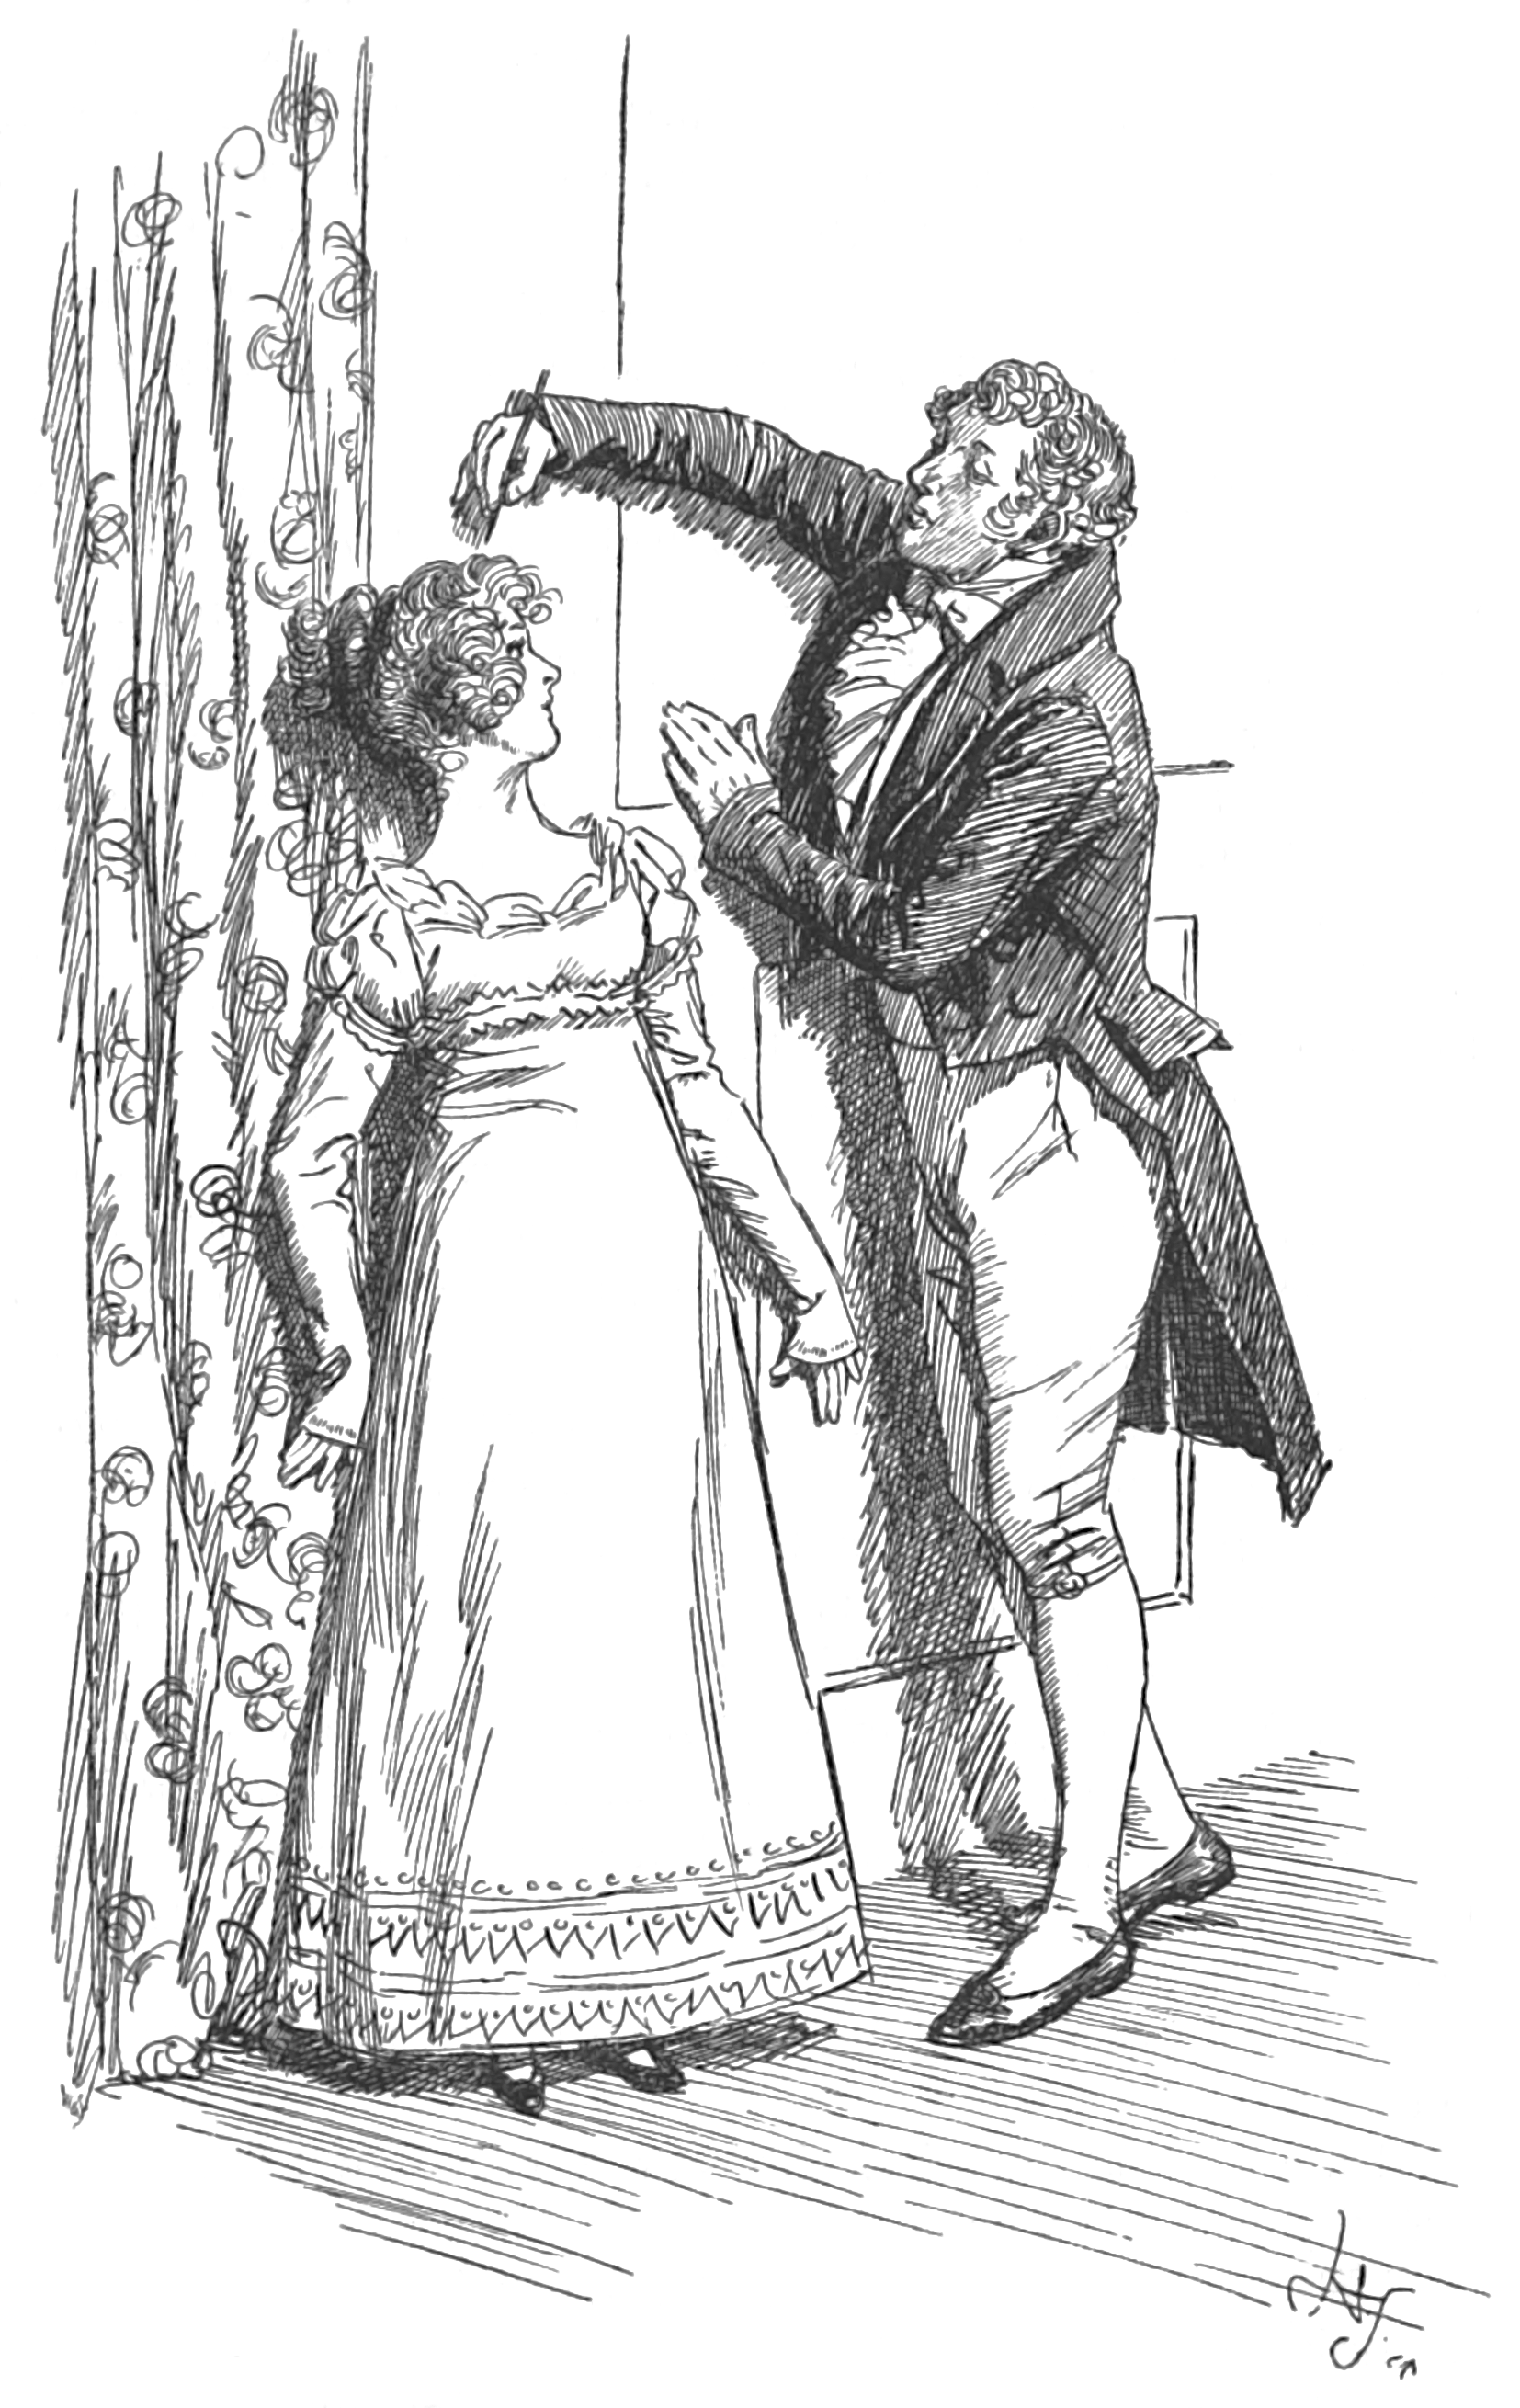
\includegraphics[width=.9\linewidth]{23room}
\caption{In that very room she had been measured}
\end{figure}

Harriet could not very soon give an intelligible account. She was feeling too much; but at last Emma collected from her enough to understand the sort of meeting, and the sort of pain it was creating. She had seen only Mrs Martin and the two girls. They had received her doubtingly, if not coolly; and nothing beyond the merest commonplace had been talked almost all the time—till just at last, when Mrs Martin's saying, all of a sudden, that she thought Miss Smith was grown, had brought on a more interesting subject, and a warmer manner. In that very room she had been measured last September, with her two friends. There were the pencilled marks and memorandums on the wainscot by the window. He had done it. They all seemed to remember the day, the hour, the party, the occasion—to feel the same consciousness, the same regrets—to be ready to return to the same good understanding; and they were just growing again like themselves, (Harriet, as Emma must suspect, as ready as the best of them to be cordial and happy,) when the carriage reappeared, and all was over. The style of the visit, and the shortness of it, were then felt to be decisive. Fourteen minutes to be given to those with whom she had thankfully passed six weeks not six months ago!—Emma could not but picture it all, and feel how justly they might resent, how naturally Harriet must suffer. It was a bad business. She would have given a great deal, or endured a great deal, to have had the Martins in a higher rank of life. They were so deserving, that a little higher should have been enough: but as it was, how could she have done otherwise?—Impossible!—She could not repent. They must be separated; but there was a great deal of pain in the process—so much to herself at this time, that she soon felt the necessity of a little consolation, and resolved on going home by way of Randalls to procure it. Her mind was quite sick of Mr Elton and the Martins. The refreshment of Randalls was absolutely necessary.

It was a good scheme; but on driving to the door they heard that neither »master nor mistress was at home;« they had both been out some time; the man believed they were gone to Hartfield.

»This is too bad,« cried Emma, as they turned away. »And now we shall just miss them; too provoking!—I do not know when I have been so disappointed.« And she leaned back in the corner, to indulge her murmurs, or to reason them away; probably a little of both—such being the commonest process of a not ill-disposed mind. Presently the carriage stopt; she looked up; it was stopt by Mr and Mrs Weston, who were standing to speak to her. There was instant pleasure in the sight of them, and still greater pleasure was conveyed in sound—for Mr Weston immediately accosted her with,

»How d'ye do?—how d'ye do?—We have been sitting with your father—glad to see him so well. Frank comes to-morrow—I had a letter this morning—we see him to-morrow by dinner-time to a certainty—he is at Oxford to-day, and he comes for a whole fortnight; I knew it would be so. If he had come at Christmas he could not have staid three days; I was always glad he did not come at Christmas; now we are going to have just the right weather for him, fine, dry, settled weather. We shall enjoy him completely; every thing has turned out exactly as we could wish.«

There was no resisting such news, no possibility of avoiding the influence of such a happy face as Mr Weston's, confirmed as it all was by the words and the countenance of his wife, fewer and quieter, but not less to the purpose. To know that she thought his coming certain was enough to make Emma consider it so, and sincerely did she rejoice in their joy. It was a most delightful reanimation of exhausted spirits. The worn-out past was sunk in the freshness of what was coming; and in the rapidity of half a moment's thought, she hoped Mr Elton would now be talked of no more.

Mr Weston gave her the history of the engagements at Enscombe, which allowed his son to answer for having an entire fortnight at his command, as well as the route and the method of his journey; and she listened, and smiled, and congratulated.

»I shall soon bring him over to Hartfield,« said he, at the conclusion.

Emma could imagine she saw a touch of the arm at this speech, from his wife.

»We had better move on, Mr Weston,« said she, »we are detaining the girls.«

»Well, well, I am ready;«—and turning again to Emma, »but you must not be expecting such a very fine young man; you have only had my account you know; I dare say he is really nothing extraordinary:«—though his own sparkling eyes at the moment were speaking a very different conviction.

Emma could look perfectly unconscious and innocent, and answer in a manner that appropriated nothing.

»Think of me to-morrow, my dear Emma, about four o'clock,« was Mrs Weston's parting injunction; spoken with some anxiety, and meant only for her.

»Four o'clock!—depend upon it he will be here by three,« was Mr Weston's quick amendment; and so ended a most satisfactory meeting. Emma's spirits were mounted quite up to happiness; every thing wore a different air; James and his horses seemed not half so sluggish as before. When she looked at the hedges, she thought the elder at least must soon be coming out; and when she turned round to Harriet, she saw something like a look of spring, a tender smile even there.

»Will Mr Frank Churchill pass through Bath as well as Oxford?«—was a question, however, which did not augur much.

But neither geography nor tranquillity could come all at once, and Emma was now in a humour to resolve that they should both come in time.

The morning of the interesting day arrived, and Mrs Weston's faithful pupil did not forget either at ten, or eleven, or twelve o'clock, that she was to think of her at four.

»My dear, dear anxious friend,«—said she, in mental soliloquy, while walking downstairs from her own room, »always overcareful for every body's comfort but your own; I see you now in all your little fidgets, going again and again into his room, to be sure that all is right.« The clock struck twelve as she passed through the hall. »'Tis twelve; I shall not forget to think of you four hours hence; and by this time to-morrow, perhaps, or a little later, I may be thinking of the possibility of their all calling here. I am sure they will bring him soon.«

She opened the parlour door, and saw two gentlemen sitting with her father—Mr Weston and his son. They had been arrived only a few minutes, and Mr Weston had scarcely finished his explanation of Frank's being a day before his time, and her father was yet in the midst of his very civil welcome and congratulations, when she appeared, to have her share of surprize, introduction, and pleasure.

The Frank Churchill so long talked of, so high in interest, was actually before her—he was presented to her, and she did not think too much had been said in his praise; he was a very good looking young man; height, air, address, all were unexceptionable, and his countenance had a great deal of the spirit and liveliness of his father's; he looked quick and sensible. She felt immediately that she should like him; and there was a well-bred ease of manner, and a readiness to talk, which convinced her that he came intending to be acquainted with her, and that acquainted they soon must be.

He had reached Randalls the evening before. She was pleased with the eagerness to arrive which had made him alter his plan, and travel earlier, later, and quicker, that he might gain half a day.

»I told you yesterday,« cried Mr Weston with exultation, »I told you all that he would be here before the time named. I remembered what I used to do myself. One cannot creep upon a journey; one cannot help getting on faster than one has planned; and the pleasure of coming in upon one's friends before the look-out begins, is worth a great deal more than any little exertion it needs.«

»It is a great pleasure where one can indulge in it,« said the young man, »though there are not many houses that I should presume on so far; but in coming home I felt I might do any thing.«

The word home made his father look on him with fresh complacency. Emma was directly sure that he knew how to make himself agreeable; the conviction was strengthened by what followed. He was very much pleased with Randalls, thought it a most admirably arranged house, would hardly allow it even to be very small, admired the situation, the walk to Highbury, Highbury itself, Hartfield still more, and professed himself to have always felt the sort of interest in the country which none but one's own country gives, and the greatest curiosity to visit it. That he should never have been able to indulge so amiable a feeling before, passed suspiciously through Emma's brain; but still, if it were a falsehood, it was a pleasant one, and pleasantly handled. His manner had no air of study or exaggeration. He did really look and speak as if in a state of no common enjoyment.

Their subjects in general were such as belong to an opening acquaintance. On his side were the inquiries,—»Was she a horsewoman?—Pleasant rides?—Pleasant walks?—Had they a large neighbourhood?—Highbury, perhaps, afforded society enough?—There were several very pretty houses in and about it.—Balls—had they balls?—Was it a musical society?«

But when satisfied on all these points, and their acquaintance proportionably advanced, he contrived to find an opportunity, while their two fathers were engaged with each other, of introducing his mother-in-law, and speaking of her with so much handsome praise, so much warm admiration, so much gratitude for the happiness she secured to his father, and her very kind reception of himself, as was an additional proof of his knowing how to please—and of his certainly thinking it worth while to try to please her. He did not advance a word of praise beyond what she knew to be thoroughly deserved by Mrs Weston; but, undoubtedly he could know very little of the matter. He understood what would be welcome; he could be sure of little else. »His father's marriage,« he said, »had been the wisest measure, every friend must rejoice in it; and the family from whom he had received such a blessing must be ever considered as having conferred the highest obligation on him.«

He got as near as he could to thanking her for Miss Taylor's merits, without seeming quite to forget that in the common course of things it was to be rather supposed that Miss Taylor had formed Miss Woodhouse's character, than Miss Woodhouse Miss Taylor's. And at last, as if resolved to qualify his opinion completely for travelling round to its object, he wound it all up with astonishment at the youth and beauty of her person.

»Elegant, agreeable manners, I was prepared for,« said he; »but I confess that, considering every thing, I had not expected more than a very tolerably well-looking woman of a certain age; I did not know that I was to find a pretty young woman in Mrs Weston.«

»You cannot see too much perfection in Mrs Weston for my feelings,« said Emma; »were you to guess her to be eighteen, I should listen with pleasure; but she would be ready to quarrel with you for using such words. Don't let her imagine that you have spoken of her as a pretty young woman.«

»I hope I should know better,« he replied; »no, depend upon it, (with a gallant bow,) that in addressing Mrs Weston I should understand whom I might praise without any danger of being thought extravagant in my terms.«

Emma wondered whether the same suspicion of what might be expected from their knowing each other, which had taken strong possession of her mind, had ever crossed his; and whether his compliments were to be considered as marks of acquiescence, or proofs of defiance. She must see more of him to understand his ways; at present she only felt they were agreeable.

She had no doubt of what Mr Weston was often thinking about. His quick eye she detected again and again glancing towards them with a happy expression; and even, when he might have determined not to look, she was confident that he was often listening.

Her own father's perfect exemption from any thought of the kind, the entire deficiency in him of all such sort of penetration or suspicion, was a most comfortable circumstance. Happily he was not farther from approving matrimony than from foreseeing it.—Though always objecting to every marriage that was arranged, he never suffered beforehand from the apprehension of any; it seemed as if he could not think so ill of any two persons' understanding as to suppose they meant to marry till it were proved against them. She blessed the favouring blindness. He could now, without the drawback of a single unpleasant surmise, without a glance forward at any possible treachery in his guest, give way to all his natural kind-hearted civility in solicitous inquiries after Mr Frank Churchill's accommodation on his journey, through the sad evils of sleeping two nights on the road, and express very genuine unmixed anxiety to know that he had certainly escaped catching cold—which, however, he could not allow him to feel quite assured of himself till after another night.

A reasonable visit paid, Mr Weston began to move.—»He must be going. He had business at the Crown about his hay, and a great many errands for Mrs Weston at Ford's, but he need not hurry any body else.« His son, too well bred to hear the hint, rose immediately also, saying,

»As you are going farther on business, sir, I will take the opportunity of paying a visit, which must be paid some day or other, and therefore may as well be paid now. I have the honour of being acquainted with a neighbour of yours, (turning to Emma,) a lady residing in or near Highbury; a family of the name of Fairfax. I shall have no difficulty, I suppose, in finding the house; though Fairfax, I believe, is not the proper name—I should rather say Barnes, or Bates. Do you know any family of that name?«

»To be sure we do,« cried his father; »Mrs Bates—we passed her house—I saw Miss Bates at the window. True, true, you are acquainted with Miss Fairfax; I remember you knew her at Weymouth, and a fine girl she is. Call upon her, by all means.«

»There is no necessity for my calling this morning,« said the young man; »another day would do as well; but there was that degree of acquaintance at Weymouth which\longdash«

»Oh! go to-day, go to-day. Do not defer it. What is right to be done cannot be done too soon. And, besides, I must give you a hint, Frank; any want of attention to her here should be carefully avoided. You saw her with the Campbells, when she was the equal of every body she mixed with, but here she is with a poor old grandmother, who has barely enough to live on. If you do not call early it will be a slight.«

The son looked convinced.

»I have heard her speak of the acquaintance,« said Emma; »she is a very elegant young woman.«

He agreed to it, but with so quiet a »Yes,« as inclined her almost to doubt his real concurrence; and yet there must be a very distinct sort of elegance for the fashionable world, if Jane Fairfax could be thought only ordinarily gifted with it.

»If you were never particularly struck by her manners before,« said she, »I think you will to-day. You will see her to advantage; see her and hear her—no, I am afraid you will not hear her at all, for she has an aunt who never holds her tongue.«

»You are acquainted with Miss Jane Fairfax, sir, are you?« said Mr Woodhouse, always the last to make his way in conversation; »then give me leave to assure you that you will find her a very agreeable young lady. She is staying here on a visit to her grandmama and aunt, very worthy people; I have known them all my life. They will be extremely glad to see you, I am sure; and one of my servants shall go with you to shew you the way.«

»My dear sir, upon no account in the world; my father can direct me.«

»But your father is not going so far; he is only going to the Crown, quite on the other side of the street, and there are a great many houses; you might be very much at a loss, and it is a very dirty walk, unless you keep on the footpath; but my coachman can tell you where you had best cross the street.«

Mr Frank Churchill still declined it, looking as serious as he could, and his father gave his hearty support by calling out, »My good friend, this is quite unnecessary; Frank knows a puddle of water when he sees it, and as to Mrs Bates's, he may get there from the Crown in a hop, step, and jump.«

They were permitted to go alone; and with a cordial nod from one, and a graceful bow from the other, the two gentlemen took leave. Emma remained very well pleased with this beginning of the acquaintance, and could now engage to think of them all at Randalls any hour of the day, with full confidence in their comfort.
%!TeX root=../sensetop.tex
\chapter[Chapter \thechapter]{}
\lettrine[lraise=0.3]{I}{n} a firm, though cautious tone, Elinor thus began.

\zz
<I should be undeserving of the confidence you have honoured me with, if I felt no desire for its continuance, or no farther curiosity on its subject. I will not apologize therefore for bringing it forward again.>

<Thank you,> cried Lucy warmly, <for breaking the ice; you have set my heart at ease by it; for I was somehow or other afraid I had offended you by what I told you that Monday.>

<Offended me! How could you suppose so? Believe me,> and Elinor spoke it with the truest sincerity, <nothing could be farther from my intention than to give you such an idea. Could you have a motive for the trust, that was not honourable and flattering to me?>

<And yet I do assure you,> replied Lucy, her little sharp eyes full of meaning, <there seemed to me to be a coldness and displeasure in your manner that made me quite uncomfortable. I felt sure that you was angry with me; and have been quarrelling with myself ever since, for having took such a liberty as to trouble you with my affairs. But I am very glad to find it was only my own fancy, and that you really do not blame me. If you knew what a consolation it was to me to relieve my heart speaking to you of what I am always thinking of every moment of my life, your compassion would make you overlook every thing else I am sure.>

<Indeed, I can easily believe that it was a very great relief to you, to acknowledge your situation to me, and be assured that you shall never have reason to repent it. Your case is a very unfortunate one; you seem to me to be surrounded with difficulties, and you will have need of all your mutual affection to support you under them. Mr Ferrars, I believe, is entirely dependent on his mother.>

<He has only two thousand pounds of his own; it would be madness to marry upon that, though for my own part, I could give up every prospect of more without a sigh. I have been always used to a very small income, and could struggle with any poverty for him; but I love him too well to be the selfish means of robbing him, perhaps, of all that his mother might give him if he married to please her. We must wait, it may be for many years. With almost every other man in the world, it would be an alarming prospect; but Edward's affection and constancy nothing can deprive me of I know.>

<That conviction must be every thing to you; and he is undoubtedly supported by the same trust in your's. If the strength of your reciprocal attachment had failed, as between many people, and under many circumstances it naturally would during a four years' engagement, your situation would have been pitiable, indeed.>

Lucy here looked up; but Elinor was careful in guarding her countenance from every expression that could give her words a suspicious tendency.

<Edward's love for me,> said Lucy, <has been pretty well put to the test, by our long, very long absence since we were first engaged, and it has stood the trial so well, that I should be unpardonable to doubt it now. I can safely say that he has never gave me one moment's alarm on that account from the first.>

Elinor hardly knew whether to smile or sigh at this assertion.

Lucy went on. <I am rather of a jealous temper too by nature, and from our different situations in life, from his being so much more in the world than me, and our continual separation, I was enough inclined for suspicion, to have found out the truth in an instant, if there had been the slightest alteration in his behaviour to me when we met, or any lowness of spirits that I could not account for, or if he had talked more of one lady than another, or seemed in any respect less happy at Longstaple than he used to be. I do not mean to say that I am particularly observant or quick-sighted in general, but in such a case I am sure I could not be deceived.>

<All this,> thought Elinor, <is very pretty; but it can impose upon neither of us.>

<But what,> said she after a short silence, <are your views? or have you none but that of waiting for Mrs Ferrars's death, which is a melancholy and shocking extremity?—Is her son determined to submit to this, and to all the tediousness of the many years of suspense in which it may involve you, rather than run the risk of her displeasure for a while by owning the truth?>

<If we could be certain that it would be only for a while! But Mrs Ferrars is a very headstrong proud woman, and in her first fit of anger upon hearing it, would very likely secure every thing to Robert, and the idea of that, for Edward's sake, frightens away all my inclination for hasty measures.>

<And for your own sake too, or you are carrying your disinterestedness beyond reason.>

Lucy looked at Elinor again, and was silent.

<Do you know Mr Robert Ferrars?> asked Elinor.

<Not at all—I never saw him; but I fancy he is very unlike his brother—silly and a great coxcomb.>

<A great coxcomb!> repeated Miss Steele, whose ear had caught those words by a sudden pause in Marianne's music. <Oh, they are talking of their favourite beaux, I dare say.>

<No sister,> cried Lucy, <you are mistaken there, our favourite beaux are \textit{not} great coxcombs.>

<I can answer for it that Miss Dashwood's is not,> said Mrs Jennings, laughing heartily; <for he is one of the modestest, prettiest behaved young men I ever saw; but as for Lucy, she is such a sly little creature, there is no finding out who \textit{she} likes.>

% \begin{figure}[tbph]
% \centering
% 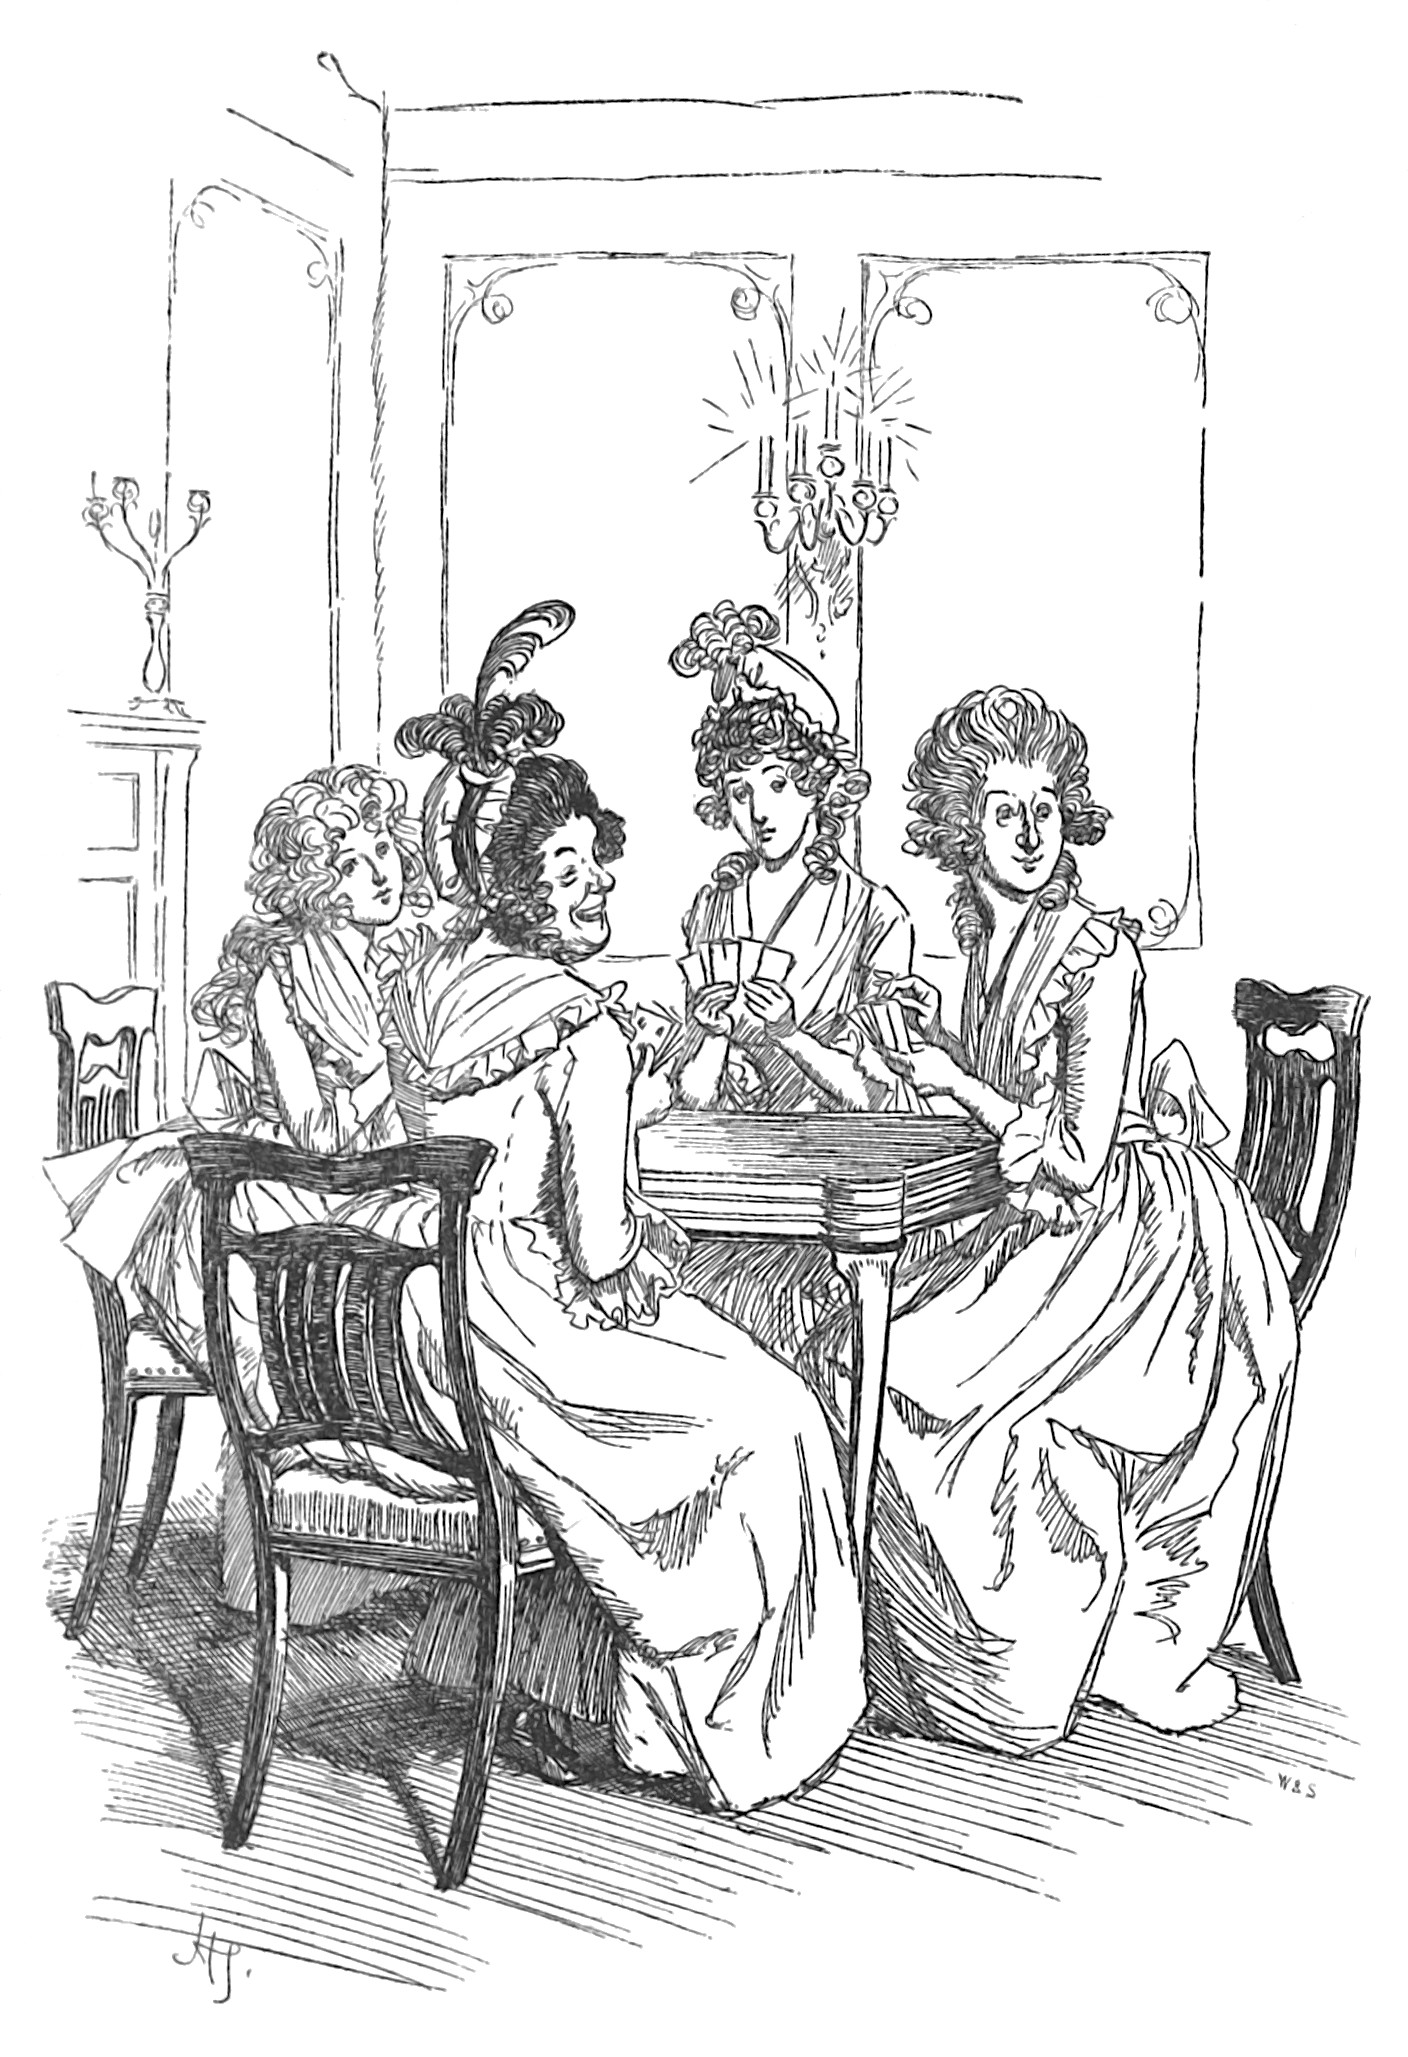
\includegraphics[width=\linewidth]{24answer}
% \caption{<I can answer for it,> said Mrs Jennings}
% \end{figure}

\begin{bwbigpic}
	[1.0]
	{24answer} 
	{<I can answer for it,> said Mrs Jennings} 
\end{bwbigpic}

<Oh,> cried Miss Steele, looking significantly round at them, <I dare say Lucy's beau is quite as modest and pretty behaved as Miss Dashwood's.>

Elinor blushed in spite of herself. Lucy bit her lip, and looked angrily at her sister. A mutual silence took place for some time. Lucy first put an end to it by saying in a lower tone, though Marianne was then giving them the powerful protection of a very magnificent concerto,—

<I will honestly tell you of one scheme which has lately come into my head, for bringing matters to bear; indeed I am bound to let you into the secret, for you are a party concerned. I dare say you have seen enough of Edward to know that he would prefer the church to every other profession; now my plan is that he should take orders as soon as he can, and then through your interest, which I am sure you would be kind enough to use out of friendship for him, and I hope out of some regard to me, your brother might be persuaded to give him Norland living; which I understand is a very good one, and the present incumbent not likely to live a great while. That would be enough for us to marry upon, and we might trust to time and chance for the rest.>

<I should always be happy,> replied Elinor, <to show any mark of my esteem and friendship for Mr Ferrars; but do you not perceive that my interest on such an occasion would be perfectly unnecessary? He is brother to Mrs John Dashwood—\textit{that} must be recommendation enough to her husband.>

<But Mrs John Dashwood would not much approve of Edward's going into orders.>

<Then I rather suspect that my interest would do very little.>

They were again silent for many minutes. At length Lucy exclaimed with a deep sigh,

<I believe it would be the wisest way to put an end to the business at once by dissolving the engagement. We seem so beset with difficulties on every side, that though it would make us miserable for a time, we should be happier perhaps in the end. But you will not give me your advice, Miss Dashwood?>

<No,> answered Elinor, with a smile, which concealed very agitated feelings, <on such a subject I certainly will not. You know very well that my opinion would have no weight with you, unless it were on the side of your wishes.>

<Indeed you wrong me,> replied Lucy, with great solemnity; <I know nobody of whose judgment I think so highly as I do of yours; and I do really believe, that if you was to say to me, <I advise you by all means to put an end to your engagement with Edward Ferrars, it will be more for the happiness of both of you,> I should resolve upon doing it immediately.>

Elinor blushed for the insincerity of Edward's future wife, and replied, <This compliment would effectually frighten me from giving any opinion on the subject had I formed one. It raises my influence much too high; the power of dividing two people so tenderly attached is too much for an indifferent person.>

<'Tis because you are an indifferent person,> said Lucy, with some pique, and laying a particular stress on those words, <that your judgment might justly have such weight with me. If you could be supposed to be biased in any respect by your own feelings, your opinion would not be worth having.>

Elinor thought it wisest to make no answer to this, lest they might provoke each other to an unsuitable increase of ease and unreserve; and was even partly determined never to mention the subject again. Another pause therefore of many minutes' duration, succeeded this speech, and Lucy was still the first to end it.

<Shall you be in town this winter, Miss Dashwood?> said she with all her accustomary complacency.

<Certainly not.>

<I am sorry for that,> returned the other, while her eyes brightened at the information, <it would have gave me such pleasure to meet you there! But I dare say you will go for all that. To be sure, your brother and sister will ask you to come to them.>

<It will not be in my power to accept their invitation if they do.>

<How unlucky that is! I had quite depended upon meeting you there. Anne and me are to go the latter end of January to some relations who have been wanting us to visit them these several years! But I only go for the sake of seeing Edward. He will be there in February, otherwise London would have no charms for me; I have not spirits for it.>

Elinor was soon called to the card-table by the conclusion of the first rubber, and the confidential discourse of the two ladies was therefore at an end, to which both of them submitted without any reluctance, for nothing had been said on either side to make them dislike each other less than they had done before; and Elinor sat down to the card table with the melancholy persuasion that Edward was not only without affection for the person who was to be his wife; but that he had not even the chance of being tolerably happy in marriage, which sincere affection on \textit{her} side would have given, for self-interest alone could induce a woman to keep a man to an engagement, of which she seemed so thoroughly aware that he was weary.

From this time the subject was never revived by Elinor, and when entered on by Lucy, who seldom missed an opportunity of introducing it, and was particularly careful to inform her confidante, of her happiness whenever she received a letter from Edward, it was treated by the former with calmness and caution, and dismissed as soon as civility would allow; for she felt such conversations to be an indulgence which Lucy did not deserve, and which were dangerous to herself.

The visit of the Miss Steeles at Barton Park was lengthened far beyond what the first invitation implied. Their favour increased; they could not be spared; Sir John would not hear of their going; and in spite of their numerous and long arranged engagements in Exeter, in spite of the absolute necessity of returning to fulfil them immediately, which was in full force at the end of every week, they were prevailed on to stay nearly two months at the park, and to assist in the due celebration of that festival which requires a more than ordinary share of private balls and large dinners to proclaim its importance.
%!TeX root=../sensetop.tex
\chapter[Chapter \thechapter]{}
\lettrine[lines=4,lraise=0.3]{T}{hough} Mrs Jennings was in the habit of spending a large portion of the year at the houses of her children and friends, she was not without a settled habitation of her own. Since the death of her husband, who had traded with success in a less elegant part of the town, she had resided every winter in a house in one of the streets near Portman Square. Towards this home, she began on the approach of January to turn her thoughts, and thither she one day abruptly, and very unexpectedly by them, asked the elder Misses Dashwood to accompany her. Elinor, without observing the varying complexion of her sister, and the animated look which spoke no indifference to the plan, immediately gave a grateful but absolute denial for both, in which she believed herself to be speaking their united inclinations. The reason alleged was their determined resolution of not leaving their mother at that time of the year. Mrs Jennings received the refusal with some surprise, and repeated her invitation immediately.

»Oh, Lord! I am sure your mother can spare you very well, and I \textit{do} beg you will favour me with your company, for I’ve quite set my heart upon it. Don’t fancy that you will be any inconvenience to me, for I shan’t put myself at all out of my way for you. It will only be sending Betty by the coach, and I hope I can afford \textit{that}. We three shall be able to go very well in my chaise; and when we are in town, if you do not like to go wherever I do, well and good, you may always go with one of my daughters. I am sure your mother will not object to it; for I have had such good luck in getting my own children off my hands that she will think me a very fit person to have the charge of you; and if I don’t get one of you at least well married before I have done with you, it shall not be my fault. I shall speak a good word for you to all the young men, you may depend upon it.«

»I have a notion,« said Sir John, »that Miss Marianne would not object to such a scheme, if her elder sister would come into it. It is very hard indeed that she should not have a little pleasure, because Miss Dashwood does not wish it. So I would advise you two, to set off for town, when you are tired of Barton, without saying a word to Miss Dashwood about it.«

»Nay,« cried Mrs Jennings, »I am sure I shall be monstrous glad of Miss Marianne’s company, whether Miss Dashwood will go or not, only the more the merrier say I, and I thought it would be more comfortable for them to be together; because, if they got tired of me, they might talk to one another, and laugh at my odd ways behind my back. But one or the other, if not both of them, I must have. Lord bless me! how do you think I can live poking by myself, I who have been always used till this winter to have Charlotte with me. Come, Miss Marianne, let us strike hands upon the bargain, and if Miss Dashwood will change her mind by and bye, why so much the better.«

»I thank you, ma’am, sincerely thank you,« said Marianne, with warmth: »your invitation has insured my gratitude for ever, and it would give me such happiness, yes, almost the greatest happiness I am capable of, to be able to accept it. But my mother, my dearest, kindest mother,—I feel the justice of what Elinor has urged, and if she were to be made less happy, less comfortable by our absence—Oh! no, nothing should tempt me to leave her. It should not, must not be a struggle.«

Mrs Jennings repeated her assurance that Mrs Dashwood could spare them perfectly well; and Elinor, who now understood her sister, and saw to what indifference to almost every thing else she was carried by her eagerness to be with Willoughby again, made no farther direct opposition to the plan, and merely referred it to her mother’s decision, from whom however she scarcely expected to receive any support in her endeavour to prevent a visit, which she could not approve of for Marianne, and which on her own account she had particular reasons to avoid. Whatever Marianne was desirous of, her mother would be eager to promote—she could not expect to influence the latter to cautiousness of conduct in an affair respecting which she had never been able to inspire her with distrust; and she dared not explain the motive of her own disinclination for going to London. That Marianne, fastidious as she was, thoroughly acquainted with Mrs Jennings’ manners, and invariably disgusted by them, should overlook every inconvenience of that kind, should disregard whatever must be most wounding to her irritable feelings, in her pursuit of one object, was such a proof, so strong, so full, of the importance of that object to her, as Elinor, in spite of all that had passed, was not prepared to witness.

On being informed of the invitation, Mrs Dashwood, persuaded that such an excursion would be productive of much amusement to both her daughters, and perceiving through all her affectionate attention to herself, how much the heart of Marianne was in it, would not hear of their declining the offer upon \textit{her} account; insisted on their both accepting it directly; and then began to foresee, with her usual cheerfulness, a variety of advantages that would accrue to them all, from this separation.

»I am delighted with the plan,« she cried, »it is exactly what I could wish. Margaret and I shall be as much benefited by it as yourselves. When you and the Middletons are gone, we shall go on so quietly and happily together with our books and our music! You will find Margaret so improved when you come back again! I have a little plan of alteration for your bedrooms too, which may now be performed without any inconvenience to any one. It is very right that you \textit{should} go to town; I would have every young woman of your condition in life acquainted with the manners and amusements of London. You will be under the care of a motherly good sort of woman, of whose kindness to you I can have no doubt. And in all probability you will see your brother, and whatever may be his faults, or the faults of his wife, when I consider whose son he is, I cannot bear to have you so wholly estranged from each other.«

»Though with your usual anxiety for our happiness,« said Elinor, »you have been obviating every impediment to the present scheme which occurred to you, there is still one objection which, in my opinion, cannot be so easily removed.«

Marianne’s countenance sunk.

»And what,« said Mrs Dashwood, »is my dear prudent Elinor going to suggest? What formidable obstacle is she now to bring forward? Do not let me hear a word about the expense of it.«

»My objection is this; though I think very well of Mrs Jennings’s heart, she is not a woman whose society can afford us pleasure, or whose protection will give us consequence.«

»That is very true,« replied her mother, »but of her society, separately from that of other people, you will scarcely have any thing at all, and you will almost always appear in public with Lady Middleton.«

»If Elinor is frightened away by her dislike of Mrs Jennings,« said Marianne, »at least it need not prevent \textsc{my} accepting her invitation. I have no such scruples, and I am sure I could put up with every unpleasantness of that kind with very little effort.«

Elinor could not help smiling at this display of indifference towards the manners of a person, to whom she had often had difficulty in persuading Marianne to behave with tolerable politeness; and resolved within herself, that if her sister persisted in going, she would go likewise, as she did not think it proper that Marianne should be left to the sole guidance of her own judgment, or that Mrs Jennings should be abandoned to the mercy of Marianne for all the comfort of her domestic hours. To this determination she was the more easily reconciled, by recollecting that Edward Ferrars, by Lucy’s account, was not to be in town before February; and that their visit, without any unreasonable abridgement, might be previously finished.

»I will have you \textit{both} go,« said Mrs Dashwood; »these objections are nonsensical. You will have much pleasure in being in London, and especially in being together; and if Elinor would ever condescend to anticipate enjoyment, she would foresee it there from a variety of sources; she would, perhaps, expect some from improving her acquaintance with her sister-in-law’s family.«

Elinor had often wished for an opportunity of attempting to weaken her mother’s dependence on the attachment of Edward and herself, that the shock might be less when the whole truth were revealed, and now on this attack, though almost hopeless of success, she forced herself to begin her design by saying, as calmly as she could, »I like Edward Ferrars very much, and shall always be glad to see him; but as to the rest of the family, it is a matter of perfect indifference to me, whether I am ever known to them or not.«

Mrs Dashwood smiled, and said nothing. Marianne lifted up her eyes in astonishment, and Elinor conjectured that she might as well have held her tongue.

After very little farther discourse, it was finally settled that the invitation should be fully accepted. Mrs Jennings received the information with a great deal of joy, and many assurances of kindness and care; nor was it a matter of pleasure merely to her. Sir John was delighted; for to a man, whose prevailing anxiety was the dread of being alone, the acquisition of two, to the number of inhabitants in London, was something. Even Lady Middleton took the trouble of being delighted, which was putting herself rather out of her way; and as for the Miss Steeles, especially Lucy, they had never been so happy in their lives as this intelligence made them.

Elinor submitted to the arrangement which counteracted her wishes with less reluctance than she had expected to feel. With regard to herself, it was now a matter of unconcern whether she went to town or not, and when she saw her mother so thoroughly pleased with the plan, and her sister exhilarated by it in look, voice, and manner, restored to all her usual animation, and elevated to more than her usual gaiety, she could not be dissatisfied with the cause, and would hardly allow herself to distrust the consequence.

Marianne’s joy was almost a degree beyond happiness, so great was the perturbation of her spirits and her impatience to be gone. Her unwillingness to quit her mother was her only restorative to calmness; and at the moment of parting her grief on that score was excessive. Her mother’s affliction was hardly less, and Elinor was the only one of the three, who seemed to consider the separation as any thing short of eternal.

Their departure took place in the first week in January. The Middletons were to follow in about a week. The Miss Steeles kept their station at the park, and were to quit it only with the rest of the family.
\chapter{Mrs~Johnson to Lady~Susan}
  
  \begin{mail}{Edward Street.}{}

I am gratified by your reference, and this is my advice: that you come to town yourself, without loss of time, but that you leave Frederica behind. It would surely be much more to the purpose to get yourself well established by marrying Mr~De Courcy, than to irritate him and the rest of his family by making her marry Sir~James. You should think more of yourself and less of your daughter. She is not of a disposition to do you credit in the world, and seems precisely in her proper place at Churchhill, with the Vernons. But you are fitted for society, and it is shameful to have you exiled from it. Leave Frederica, therefore, to punish herself for the plague she has given you, by indulging that romantic tender-heartedness which will always ensure her misery enough, and come to London as soon as you can. I have another reason for urging this: Mainwaring came to town last week, and has contrived, in spite of Mr~Johnson, to make opportunities of seeing me. He is absolutely miserable about you, and jealous to such a degree of De Courcy that it would be highly unadvisable for them to meet at present. And yet, if you do not allow him to see you here, I cannot answer for his not committing some great imprudence—such as going to Churchhill, for instance, which would be dreadful! Besides, if you take my advice, and resolve to marry De Courcy, it will be indispensably necessary to you to get Mainwaring out of the way; and you only can have influence enough to send him back to his wife. I have still another motive for your coming: Mr~Johnson leaves London next Tuesday; he is going for his health to Bath, where, if the waters are favourable to his constitution and my wishes, he will be laid up with the gout many weeks. During his absence we shall be able to chuse our own society, and to have true enjoyment. I would ask you to Edward Street, but that once he forced from me a kind of promise never to invite you to my house; nothing but my being in the utmost distress for money should have extorted it from me. I can get you, however, a nice drawing-room apartment in Upper Seymour Street, and we may be always together there or here; for I consider my promise to Mr~Johnson as comprehending only (at least in his absence) your not sleeping in the house. Poor Mainwaring gives me such histories of his wife's jealousy. Silly woman to expect constancy from so charming a man! but she always was silly—intolerably so in marrying him at all, she the heiress of a large fortune and he without a shilling: one title, I know, she might have had, besides baronets. Her folly in forming the connection was so great that, though Mr~Johnson was her guardian, and I do not in general share \textit{his} feelings, I never can forgive her. 

\closeletter[Adieu. Yours ever,]{Alicia.} 
\end{mail}
\chapter{Mrs~Vernon to Lady~De Courcy}
  
  \begin{mail}{Churchhill.}{}

This letter, my dear Mother, will be brought you by Reginald. His long visit is about to be concluded at last, but I fear the separation takes place too late to do us any good. She is going to London to see her particular friend, Mrs~Johnson. It was at first her intention that Frederica should accompany her, for the benefit of masters, but we overruled her there. Frederica was wretched in the idea of going, and I could not bear to have her at the mercy of her mother; not all the masters in London could compensate for the ruin of her comfort. I should have feared, too, for her health, and for everything but her principles—there I believe she is not to be injured by her mother, or her mother's friends; but with those friends she must have mixed (a very bad set, I doubt not), or have been left in total solitude, and I can hardly tell which would have been worse for her. If she is with her mother, moreover, she must, alas! in all probability be with Reginald, and that would be the greatest evil of all. Here we shall in time be in peace, and our regular employments, our books and conversations, with exercise, the children, and every domestic pleasure in my power to procure her, will, I trust, gradually overcome this youthful attachment. I should not have a doubt of it were she slighted for any other woman in the world than her own mother. How long Lady~Susan will be in town, or whether she returns here again, I know not. I could not be cordial in my invitation, but if she chuses to come no want of cordiality on my part will keep her away. I could not help asking Reginald if he intended being in London this winter, as soon as I found her ladyship's steps would be bent thither; and though he professed himself quite undetermined, there was something in his look and voice as he spoke which contradicted his words. I have done with lamentation; I look upon the event as so far decided that I resign myself to it in despair. If he leaves you soon for London everything will be concluded. 

\closeletter[Your affectionate, \&c.,]{C. Vernon.} 
\end{mail}
%!TeX root=../emmatop.tex
\chapter[Chapter \thechapter]{}
\lettrine[lines=4,lraise=0.3]{T}{he} appearance of the little sitting-room as they entered, was tranquillity itself; Mrs Bates, deprived of her usual employment, slumbering on one side of the fire, Frank Churchill, at a table near her, most deedily occupied about her spectacles, and Jane Fairfax, standing with her back to them, intent on her pianoforte.

\begin{figure}[tbph]
\centering
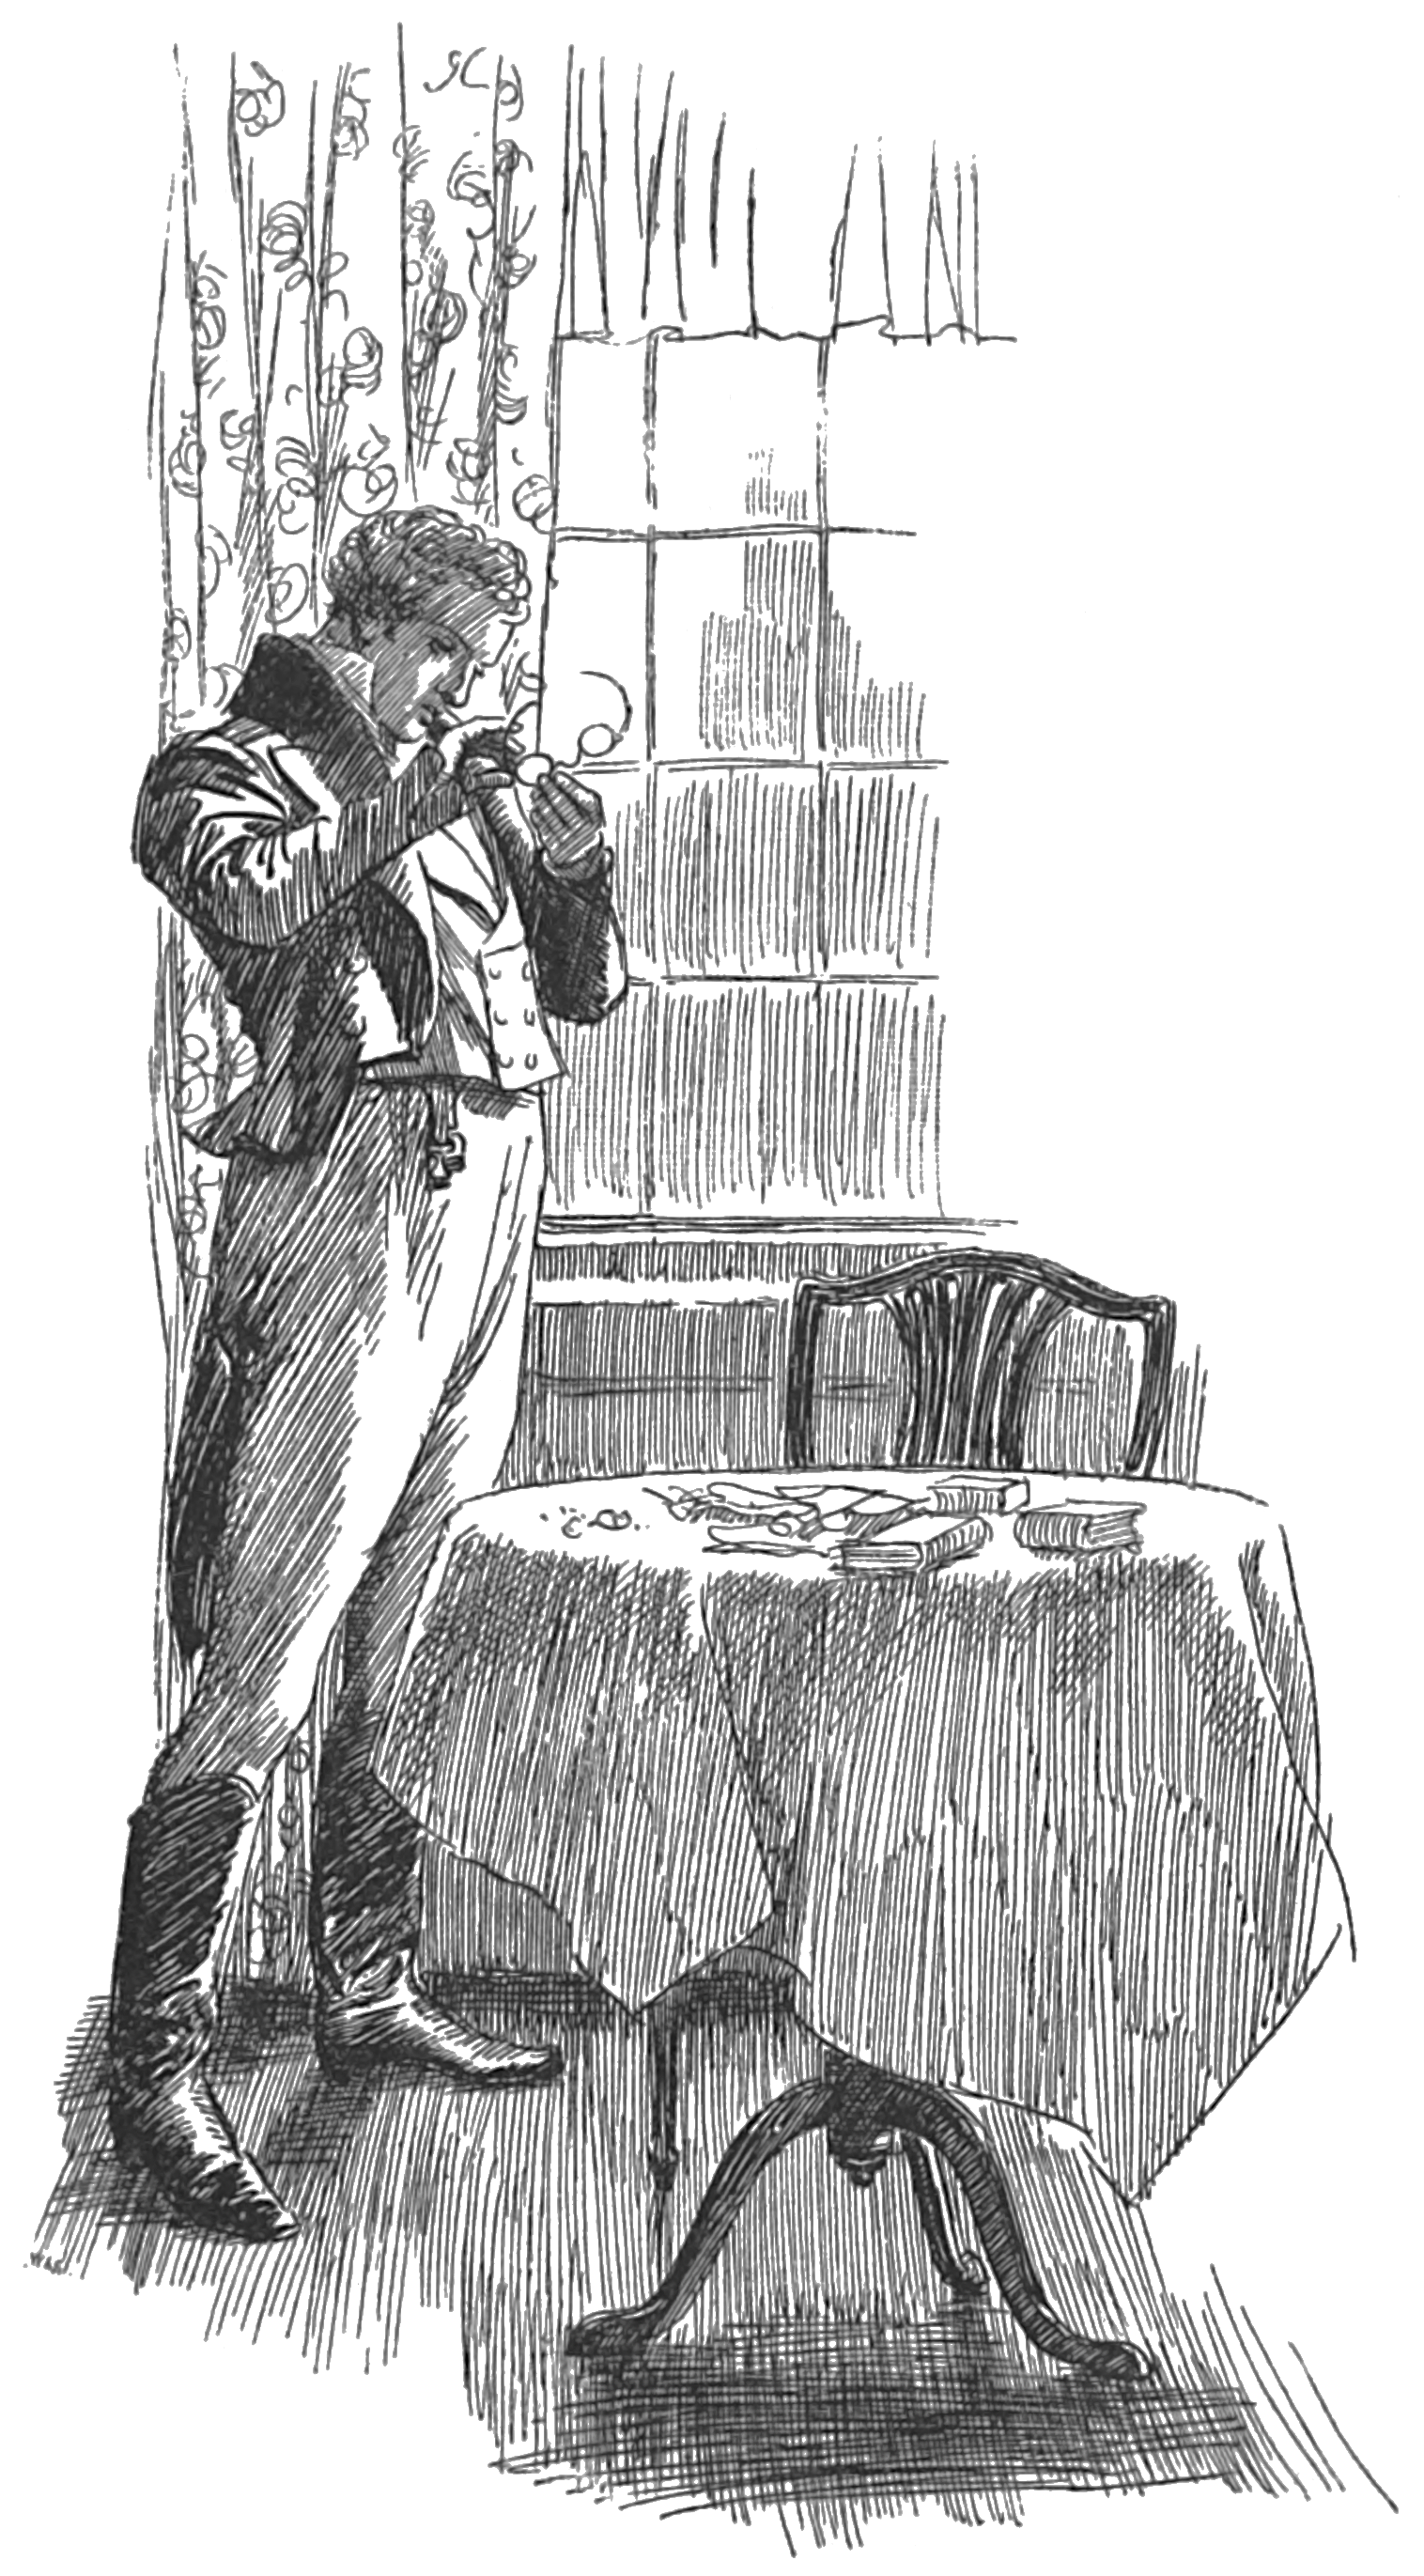
\includegraphics[width=.8\linewidth]{28spectacles}
\caption{Occupied about her spectacles}
\end{figure}

Busy as he was, however, the young man was yet able to shew a most happy countenance on seeing Emma again.

»This is a pleasure,« said he, in rather a low voice, »coming at least ten minutes earlier than I had calculated. You find me trying to be useful; tell me if you think I shall succeed.«

»What!« said Mrs Weston, »have not you finished it yet? you would not earn a very good livelihood as a working silversmith at this rate.«

»I have not been working uninterruptedly,« he replied, »I have been assisting Miss Fairfax in trying to make her instrument stand steadily, it was not quite firm; an unevenness in the floor, I believe. You see we have been wedging one leg with paper. This was very kind of you to be persuaded to come. I was almost afraid you would be hurrying home.«

He contrived that she should be seated by him; and was sufficiently employed in looking out the best baked apple for her, and trying to make her help or advise him in his work, till Jane Fairfax was quite ready to sit down to the pianoforte again. That she was not immediately ready, Emma did suspect to arise from the state of her nerves; she had not yet possessed the instrument long enough to touch it without emotion; she must reason herself into the power of performance; and Emma could not but pity such feelings, whatever their origin, and could not but resolve never to expose them to her neighbour again.

At last Jane began, and though the first bars were feebly given, the powers of the instrument were gradually done full justice to. Mrs Weston had been delighted before, and was delighted again; Emma joined her in all her praise; and the pianoforte, with every proper discrimination, was pronounced to be altogether of the highest promise.

»Whoever Colonel Campbell might employ,« said Frank Churchill, with a smile at Emma, »the person has not chosen ill. I heard a good deal of Colonel Campbell's taste at Weymouth; and the softness of the upper notes I am sure is exactly what he and all that party would particularly prize. I dare say, Miss Fairfax, that he either gave his friend very minute directions, or wrote to Broadwood himself. Do not you think so?«

Jane did not look round. She was not obliged to hear. Mrs Weston had been speaking to her at the same moment.

»It is not fair,« said Emma, in a whisper; »mine was a random guess. Do not distress her.«

He shook his head with a smile, and looked as if he had very little doubt and very little mercy. Soon afterwards he began again,

»How much your friends in Ireland must be enjoying your pleasure on this occasion, Miss Fairfax. I dare say they often think of you, and wonder which will be the day, the precise day of the instrument's coming to hand. Do you imagine Colonel Campbell knows the business to be going forward just at this time?—Do you imagine it to be the consequence of an immediate commission from him, or that he may have sent only a general direction, an order indefinite as to time, to depend upon contingencies and conveniences?«

He paused. She could not but hear; she could not avoid answering,

»Till I have a letter from Colonel Campbell,« said she, in a voice of forced calmness, »I can imagine nothing with any confidence. It must be all conjecture.«

»Conjecture—aye, sometimes one conjectures right, and sometimes one conjectures wrong. I wish I could conjecture how soon I shall make this rivet quite firm. What nonsense one talks, Miss Woodhouse, when hard at work, if one talks at all;—your real workmen, I suppose, hold their tongues; but we gentlemen labourers if we get hold of a word—Miss Fairfax said something about conjecturing. There, it is done. I have the pleasure, madam, (to Mrs Bates,) of restoring your spectacles, healed for the present.«

He was very warmly thanked both by mother and daughter; to escape a little from the latter, he went to the pianoforte, and begged Miss Fairfax, who was still sitting at it, to play something more.

»If you are very kind,« said he, »it will be one of the waltzes we danced last night;—let me live them over again. You did not enjoy them as I did; you appeared tired the whole time. I believe you were glad we danced no longer; but I would have given worlds—all the worlds one ever has to give—for another half-hour.«

She played.

»What felicity it is to hear a tune again which has made one happy!—If I mistake not that was danced at Weymouth.«

She looked up at him for a moment, coloured deeply, and played something else. He took some music from a chair near the pianoforte, and turning to Emma, said,

»Here is something quite new to me. Do you know it?—Cramer.—And here are a new set of Irish melodies. That, from such a quarter, one might expect. This was all sent with the instrument. Very thoughtful of Colonel Campbell, was not it?—He knew Miss Fairfax could have no music here. I honour that part of the attention particularly; it shews it to have been so thoroughly from the heart. Nothing hastily done; nothing incomplete. True affection only could have prompted it.«

Emma wished he would be less pointed, yet could not help being amused; and when on glancing her eye towards Jane Fairfax she caught the remains of a smile, when she saw that with all the deep blush of consciousness, there had been a smile of secret delight, she had less scruple in the amusement, and much less compunction with respect to her.—This amiable, upright, perfect Jane Fairfax was apparently cherishing very reprehensible feelings.

He brought all the music to her, and they looked it over together.—Emma took the opportunity of whispering,

»You speak too plain. She must understand you.«

»I hope she does. I would have her understand me. I am not in the least ashamed of my meaning.«

»But really, I am half ashamed, and wish I had never taken up the idea.«

»I am very glad you did, and that you communicated it to me. I have now a key to all her odd looks and ways. Leave shame to her. If she does wrong, she ought to feel it.«

»She is not entirely without it, I think.«

»I do not see much sign of it. She is playing Robin Adair at this moment—his favourite.«

Shortly afterwards Miss Bates, passing near the window, descried Mr Knightley on horse-back not far off.

»Mr Knightley I declare!—I must speak to him if possible, just to thank him. I will not open the window here; it would give you all cold; but I can go into my mother's room you know. I dare say he will come in when he knows who is here. Quite delightful to have you all meet so!—Our little room so honoured!«

She was in the adjoining chamber while she still spoke, and opening the casement there, immediately called Mr Knightley's attention, and every syllable of their conversation was as distinctly heard by the others, as if it had passed within the same apartment.

»How d' ye do?—how d'ye do?—Very well, I thank you. So obliged to you for the carriage last night. We were just in time; my mother just ready for us. Pray come in; do come in. You will find some friends here.«

So began Miss Bates; and Mr Knightley seemed determined to be heard in his turn, for most resolutely and commandingly did he say,

»How is your niece, Miss Bates?—I want to inquire after you all, but particularly your niece. How is Miss Fairfax?—I hope she caught no cold last night. How is she to-day? Tell me how Miss Fairfax is.«

And Miss Bates was obliged to give a direct answer before he would hear her in any thing else. The listeners were amused; and Mrs Weston gave Emma a look of particular meaning. But Emma still shook her head in steady scepticism.

»So obliged to you!—so very much obliged to you for the carriage,« resumed Miss Bates.

He cut her short with,

»I am going to Kingston. Can I do any thing for you?«

»Oh! dear, Kingston—are you?—Mrs Cole was saying the other day she wanted something from Kingston.«

»Mrs Cole has servants to send. Can I do any thing for you?«

»No, I thank you. But do come in. Who do you think is here?—Miss Woodhouse and Miss Smith; so kind as to call to hear the new pianoforte. Do put up your horse at the Crown, and come in.«

»Well,« said he, in a deliberating manner, »for five minutes, perhaps.«

»And here is Mrs Weston and Mr Frank Churchill too!—Quite delightful; so many friends!«

»No, not now, I thank you. I could not stay two minutes. I must get on to Kingston as fast as I can.«

»Oh! do come in. They will be so very happy to see you.«

»No, no; your room is full enough. I will call another day, and hear the pianoforte.«

»Well, I am so sorry!—Oh! Mr Knightley, what a delightful party last night; how extremely pleasant.—Did you ever see such dancing?—Was not it delightful?—Miss Woodhouse and Mr Frank Churchill; I never saw any thing equal to it.«

»Oh! very delightful indeed; I can say nothing less, for I suppose Miss Woodhouse and Mr Frank Churchill are hearing every thing that passes. And (raising his voice still more) I do not see why Miss Fairfax should not be mentioned too. I think Miss Fairfax dances very well; and Mrs Weston is the very best country-dance player, without exception, in England. Now, if your friends have any gratitude, they will say something pretty loud about you and me in return; but I cannot stay to hear it.«


\begin{figure}[tbph]
\centering
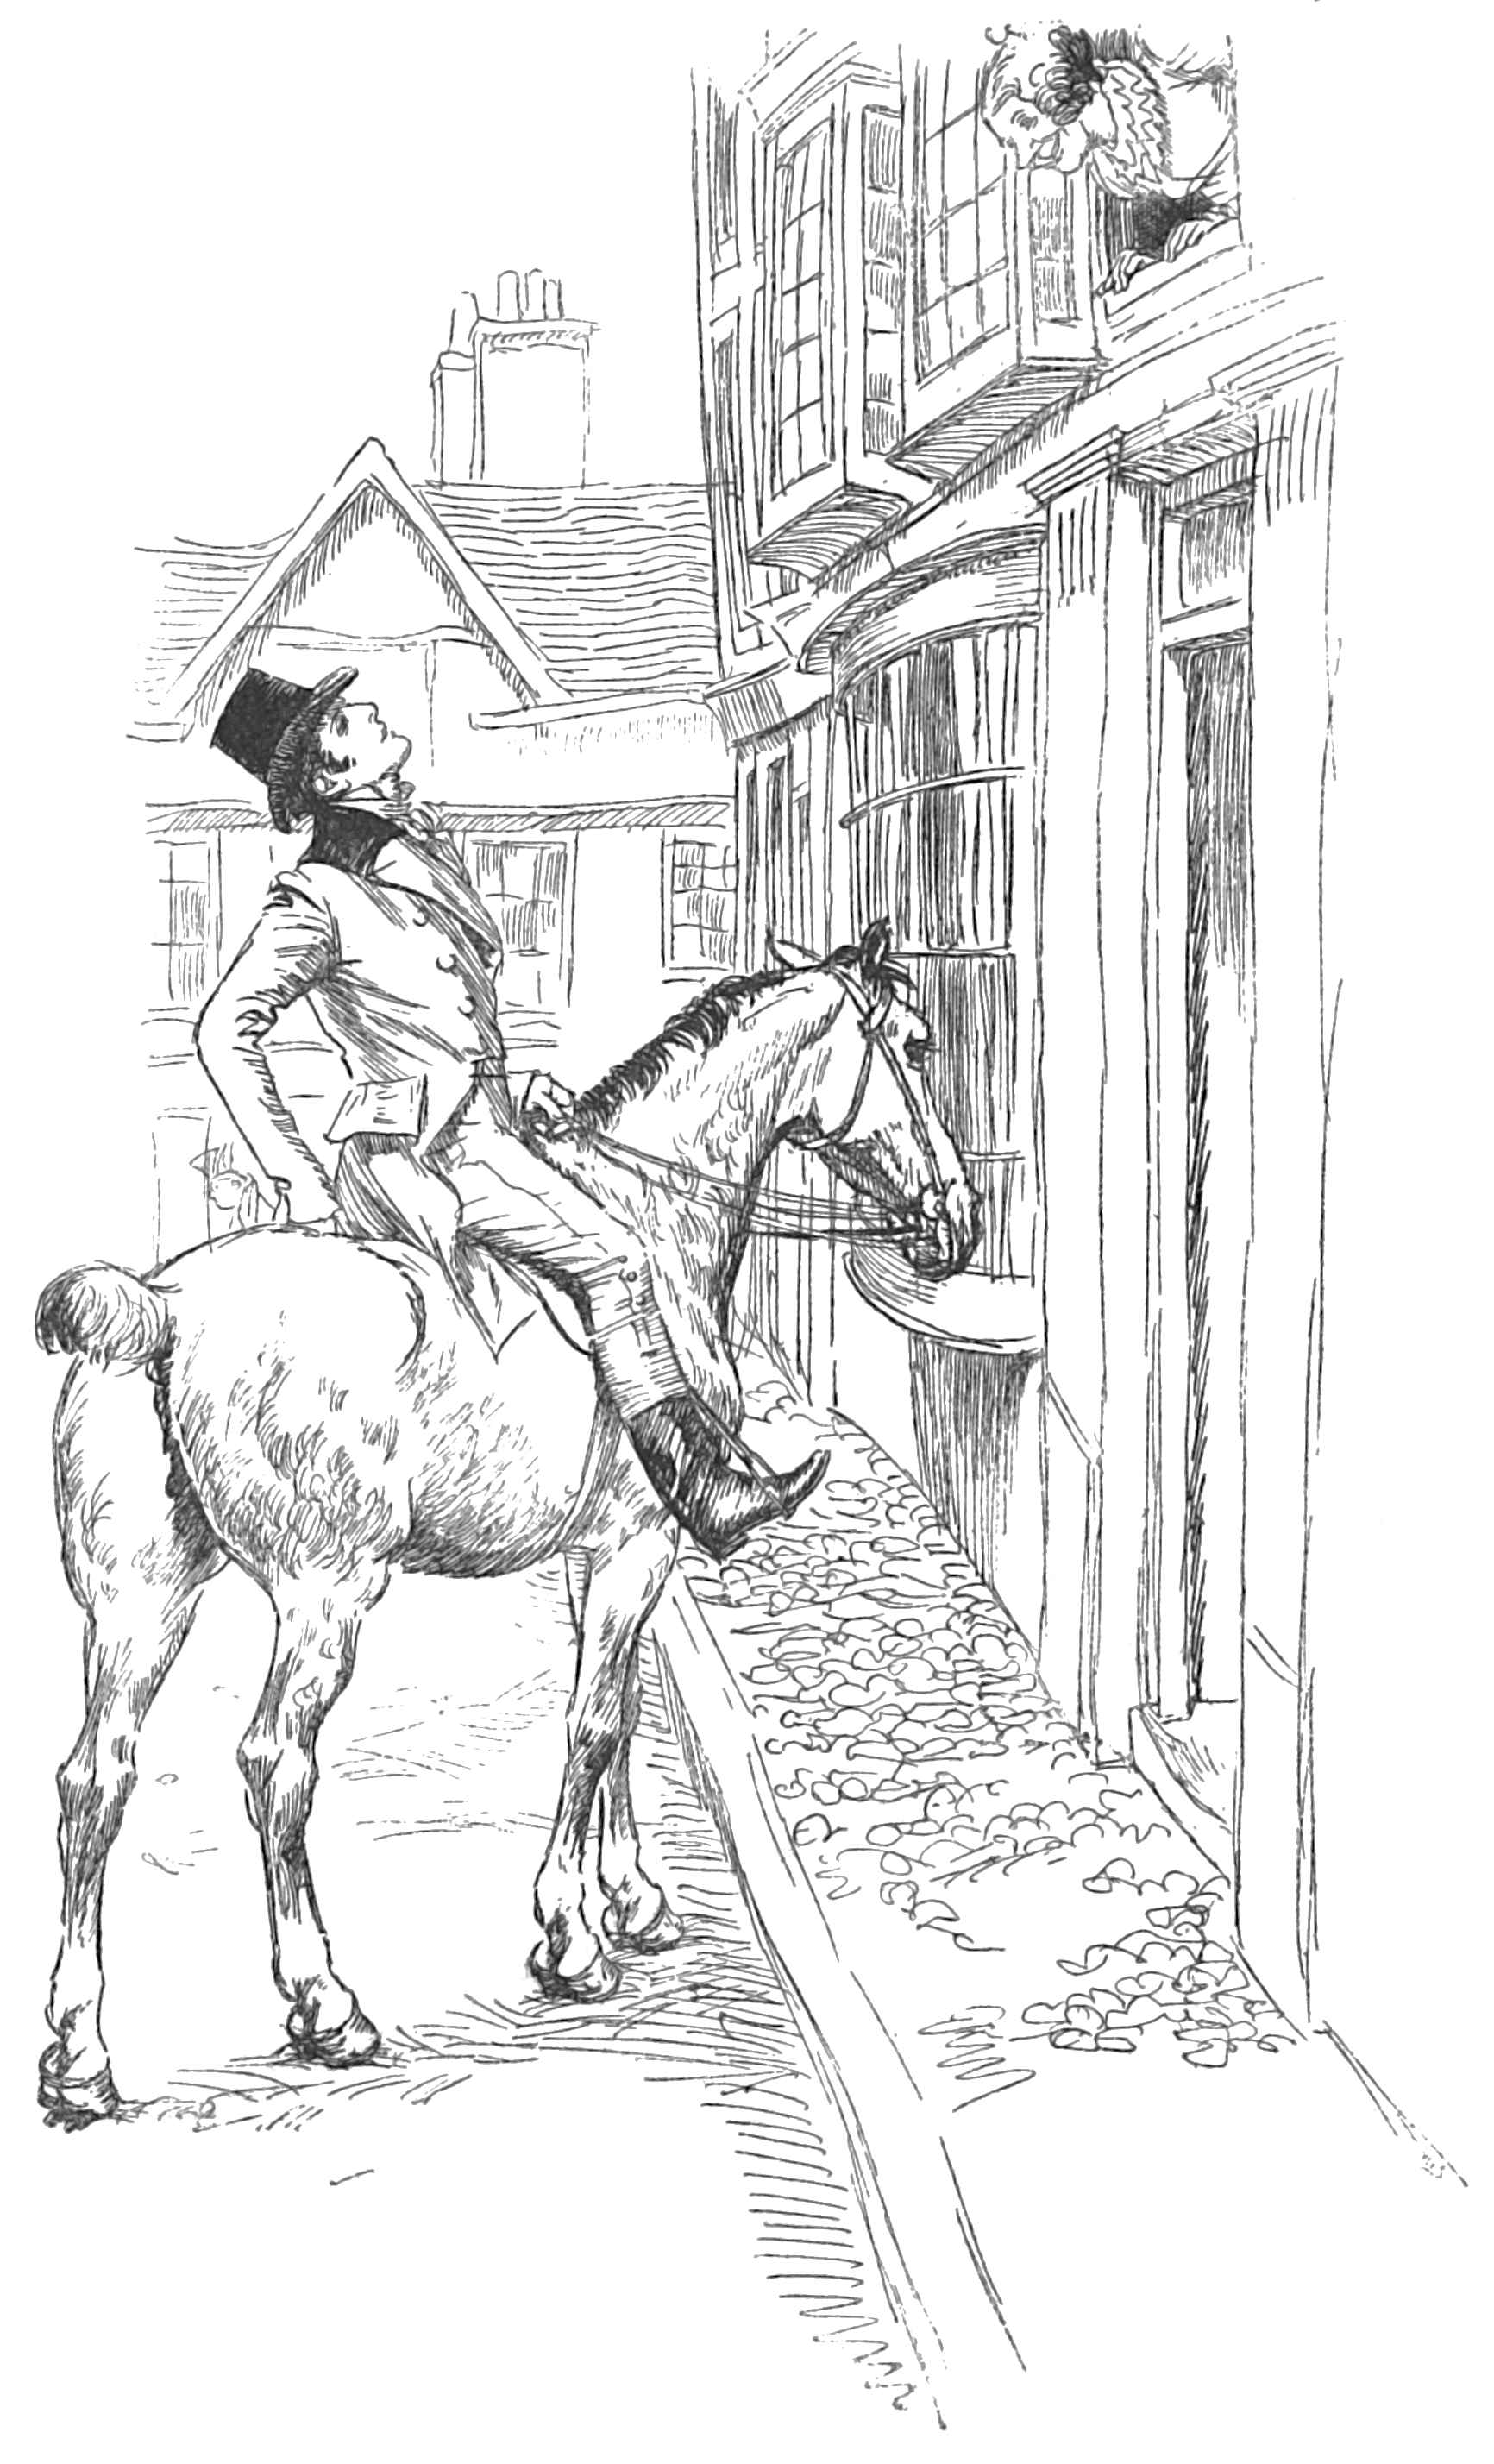
\includegraphics[width=.8\linewidth]{28moment}
\caption{»Oh! Mr Knightley, one moment more«}
\end{figure}

»Oh! Mr Knightley, one moment more; something of consequence—so shocked!—Jane and I are both so shocked about the apples!«

»What is the matter now?«

»To think of your sending us all your store apples. You said you had a great many, and now you have not one left. We really are so shocked! Mrs Hodges may well be angry. William Larkins mentioned it here. You should not have done it, indeed you should not. Ah! he is off. He never can bear to be thanked. But I thought he would have staid now, and it would have been a pity not to have mentioned.... Well, (returning to the room,) I have not been able to succeed. Mr Knightley cannot stop. He is going to Kingston. He asked me if he could do any thing....«

»Yes,« said Jane, »we heard his kind offers, we heard every thing.«

»Oh! yes, my dear, I dare say you might, because you know, the door was open, and the window was open, and Mr Knightley spoke loud. You must have heard every thing to be sure. »Can I do any thing for you at Kingston?« said he; so I just mentioned.... Oh! Miss Woodhouse, must you be going?—You seem but just come—so very obliging of you.«

Emma found it really time to be at home; the visit had already lasted long; and on examining watches, so much of the morning was perceived to be gone, that Mrs Weston and her companion taking leave also, could allow themselves only to walk with the two young ladies to Hartfield gates, before they set off for Randalls.
\chapter[Chapter \thechapter]{} 

 \lettrine[lraise=0.3]{T}{he} ball was over, and the breakfast was soon over too; the last kiss was given, and William was gone. Mr~Crawford had, as he foretold, been very punctual, and short and pleasant had been the meal.

After seeing William to the last moment, Fanny walked back to the breakfast-room with a very saddened heart to grieve over the melancholy change; and there her uncle kindly left her to cry in peace, conceiving, perhaps, that the deserted chair of each young man might exercise her tender enthusiasm, and that the remaining cold pork bones and mustard in William's plate might but divide her feelings with the broken egg-shells in Mr~Crawford's. She sat and cried \textit{con}  \textit{amore}  as her uncle intended, but it was \textit{con}  \textit{amore}  fraternal and no other. William was gone, and she now felt as if she had wasted half his visit in idle cares and selfish solicitudes unconnected with him.

Fanny's disposition was such that she could never even think of her aunt Norris in the meagreness and cheerlessness of her own small house, without reproaching herself for some little want of attention to her when they had been last together; much less could her feelings acquit her of having done and said and thought everything by William that was due to him for a whole fortnight.

It was a heavy, melancholy day. Soon after the second breakfast, Edmund bade them good-bye for a week, and mounted his horse for Peterborough, and then all were gone. Nothing remained of last night but remembrances, which she had nobody to share in. She talked to her aunt Bertram—she must talk to somebody of the ball; but her aunt had seen so little of what had passed, and had so little curiosity, that it was heavy work. Lady Bertram was not certain of anybody's dress or anybody's place at supper but her own. <She could not recollect what it was that she had heard about one of the Miss~Maddoxes, or what it was that Lady Prescott had noticed in Fanny: she was not sure whether Colonel Harrison had been talking of Mr~Crawford or of William when he said he was the finest young man in the room—somebody had whispered something to her; she had forgot to ask Sir~Thomas what it could be.> And these were her longest speeches and clearest communications: the rest was only a languid <Yes, yes; very well; did you? did he? I did not see \textit{that}; I should not know one from the other.> This was very bad. It was only better than Mrs~Norris's sharp answers would have been; but she being gone home with all the supernumerary jellies to nurse a sick maid, there was peace and good-humour in their little party, though it could not boast much beside.

The evening was heavy like the day. <I cannot think what is the matter with me,> said Lady Bertram, when the tea-things were removed. <I feel quite stupid. It must be sitting up so late last night. Fanny, you must do something to keep me awake. I cannot work. Fetch the cards; I feel so very stupid.>

The cards were brought, and Fanny played at cribbage with her aunt till bedtime; and as Sir~Thomas was reading to himself, no sounds were heard in the room for the next two hours beyond the reckonings of the game—<And \textit{that}  makes thirty-one; four in hand and eight in crib. You are to deal, ma'am; shall I deal for you?> Fanny thought and thought again of the difference which twenty-four hours had made in that room, and all that part of the house. Last night it had been hope and smiles, bustle and motion, noise and brilliancy, in the drawing-room, and out of the drawing-room, and everywhere. Now it was languor, and all but solitude.

A good night's rest improved her spirits. She could think of William the next day more cheerfully; and as the morning afforded her an opportunity of talking over Thursday night with Mrs~Grant and Miss~Crawford, in a very handsome style, with all the heightenings of imagination, and all the laughs of playfulness which are so essential to the shade of a departed ball, she could afterwards bring her mind without much effort into its everyday state, and easily conform to the tranquillity of the present quiet week.

They were indeed a smaller party than she had ever known there for a whole day together, and \textit{he}  was gone on whom the comfort and cheerfulness of every family meeting and every meal chiefly depended. But this must be learned to be endured. He would soon be always gone; and she was thankful that she could now sit in the same room with her uncle, hear his voice, receive his questions, and even answer them, without such wretched feelings as she had formerly known.

<We miss our two young men,> was Sir~Thomas's observation on both the first and second day, as they formed their very reduced circle after dinner; and in consideration of Fanny's swimming eyes, nothing more was said on the first day than to drink their good health; but on the second it led to something farther. William was kindly commended and his promotion hoped for. <And there is no reason to suppose,> added Sir~Thomas, <but that his visits to us may now be tolerably frequent. As to Edmund, we must learn to do without him. This will be the last winter of his belonging to us, as he has done.>

<Yes,> said Lady Bertram, <but I wish he was not going away. They are all going away, I think. I wish they would stay at home.>

This wish was levelled principally at Julia, who had just applied for permission to go to town with Maria; and as Sir~Thomas thought it best for each daughter that the permission should be granted, Lady Bertram, though in her own good-nature she would not have prevented it, was lamenting the change it made in the prospect of Julia's return, which would otherwise have taken place about this time. A great deal of good sense followed on Sir~Thomas's side, tending to reconcile his wife to the arrangement. Everything that a considerate parent \textit{ought}  to feel was advanced for her use; and everything that an affectionate mother \textit{must}  feel in promoting her children's enjoyment was attributed to her nature. Lady Bertram agreed to it all with a calm <Yes>; and at the end of a quarter of an hour's silent consideration spontaneously observed, <Sir~Thomas, I have been thinking—and I am very glad we took Fanny as we did, for now the others are away we feel the good of it.>

Sir~Thomas immediately improved this compliment by adding, <Very true. We shew Fanny what a good girl we think her by praising her to her face, she is now a very valuable companion. If we have been kind to \textit{her}, she is now quite as necessary to \textit{us}.>

<Yes,> said Lady Bertram presently; <and it is a comfort to think that we shall always have \textit{her}.>

Sir~Thomas paused, half smiled, glanced at his niece, and then gravely replied, <She will never leave us, I hope, till invited to some other home that may reasonably promise her greater happiness than she knows here.>

<And \textit{that}  is not very likely to be, Sir~Thomas. Who should invite her? Maria might be very glad to see her at Sotherton now and then, but she would not think of asking her to live there; and I am sure she is better off here; and besides, I cannot do without her.>

The week which passed so quietly and peaceably at the great house in Mansfield had a very different character at the Parsonage. To the young lady, at least, in each family, it brought very different feelings. What was tranquillity and comfort to Fanny was tediousness and vexation to Mary. Something arose from difference of disposition and habit: one so easily satisfied, the other so unused to endure; but still more might be imputed to difference of circumstances. In some points of interest they were exactly opposed to each other. To Fanny's mind, Edmund's absence was really, in its cause and its tendency, a relief. To Mary it was every way painful. She felt the want of his society every day, almost every hour, and was too much in want of it to derive anything but irritation from considering the object for which he went. He could not have devised anything more likely to raise his consequence than this week's absence, occurring as it did at the very time of her brother's going away, of William Price's going too, and completing the sort of general break-up of a party which had been so animated. She felt it keenly. They were now a miserable trio, confined within doors by a series of rain and snow, with nothing to do and no variety to hope for. Angry as she was with Edmund for adhering to his own notions, and acting on them in defiance of her (and she had been so angry that they had hardly parted friends at the ball), she could not help thinking of him continually when absent, dwelling on his merit and affection, and longing again for the almost daily meetings they lately had. His absence was unnecessarily long. He should not have planned such an absence—he should not have left home for a week, when her own departure from Mansfield was so near. Then she began to blame herself. She wished she had not spoken so warmly in their last conversation. She was afraid she had used some strong, some contemptuous expressions in speaking of the clergy, and that should not have been. It was ill-bred; it was wrong. She wished such words unsaid with all her heart.

Her vexation did not end with the week. All this was bad, but she had still more to feel when Friday came round again and brought no Edmund; when Saturday came and still no Edmund; and when, through the slight communication with the other family which Sunday produced, she learned that he had actually written home to defer his return, having promised to remain some days longer with his friend.

If she had felt impatience and regret before—if she had been sorry for what she said, and feared its too strong effect on him—she now felt and feared it all tenfold more. She had, moreover, to contend with one disagreeable emotion entirely new to her—jealousy. His friend Mr~Owen had sisters; he might find them attractive. But, at any rate, his staying away at a time when, according to all preceding plans, she was to remove to London, meant something that she could not bear. Had Henry returned, as he talked of doing, at the end of three or four days, she should now have been leaving Mansfield. It became absolutely necessary for her to get to Fanny and try to learn something more. She could not live any longer in such solitary wretchedness; and she made her way to the Park, through difficulties of walking which she had deemed unconquerable a week before, for the chance of hearing a little in addition, for the sake of at least hearing his name.

The first half-hour was lost, for Fanny and Lady Bertram were together, and unless she had Fanny to herself she could hope for nothing. But at last Lady Bertram left the room, and then almost immediately Miss~Crawford thus began, with a voice as well regulated as she could—<And how do \textit{you}  like your cousin Edmund's staying away so long? Being the only young person at home, I consider \textit{you}  as the greatest sufferer. You must miss him. Does his staying longer surprise you?>

<I do not know,> said Fanny hesitatingly. <Yes; I had not particularly expected it.>

<Perhaps he will always stay longer than he talks of. It is the general way all young men do.>

<He did not, the only time he went to see Mr~Owen before.>

<He finds the house more agreeable \textit{now}. He is a very—a very pleasing young man himself, and I cannot help being rather concerned at not seeing him again before I go to London, as will now undoubtedly be the case. I am looking for Henry every day, and as soon as he comes there will be nothing to detain me at Mansfield. I should like to have seen him once more, I confess. But you must give my compliments to him. Yes; I think it must be compliments. Is not there a something wanted, Miss~Price, in our language—a something between compliments and—and love—to suit the sort of friendly acquaintance we have had together? So many months' acquaintance! But compliments may be sufficient here. Was his letter a long one? Does he give you much account of what he is doing? Is it Christmas gaieties that he is staying for?>

<I only heard a part of the letter; it was to my uncle; but I believe it was very short; indeed I am sure it was but a few lines. All that I heard was that his friend had pressed him to stay longer, and that he had agreed to do so. A \textit{few}  days longer, or \textit{some}  days longer; I am not quite sure which.>

<Oh! if he wrote to his father; but I thought it might have been to Lady Bertram or you. But if he wrote to his father, no wonder he was concise. Who could write chat to Sir~Thomas? If he had written to you, there would have been more particulars. You would have heard of balls and parties. He would have sent you a description of everything and everybody. How many Miss~Owens are there?>

<Three grown up.>

<Are they musical?>

<I do not at all know. I never heard.>

<That is the first question, you know,> said Miss~Crawford, trying to appear gay and unconcerned, <which every woman who plays herself is sure to ask about another. But it is very foolish to ask questions about any young ladies—about any three sisters just grown up; for one knows, without being told, exactly what they are: all very accomplished and pleasing, and one very pretty. There is a beauty in every family; it is a regular thing. Two play on the pianoforte, and one on the harp; and all sing, or would sing if they were taught, or sing all the better for not being taught; or something like it.>

<I know nothing of the Miss~Owens,> said Fanny calmly.

<You know nothing and you care less, as people say. Never did tone express indifference plainer. Indeed, how can one care for those one has never seen? Well, when your cousin comes back, he will find Mansfield very quiet; all the noisy ones gone, your brother and mine and myself. I do not like the idea of leaving Mrs~Grant now the time draws near. She does not like my going.>

Fanny felt obliged to speak. <You cannot doubt your being missed by many,> said she. <You will be very much missed.>

Miss~Crawford turned her eye on her, as if wanting to hear or see more, and then laughingly said, <Oh yes! missed as every noisy evil is missed when it is taken away; that is, there is a great difference felt. But I am not fishing; don't compliment me. If I \textit{am}  missed, it will appear. I may be discovered by those who want to see me. I shall not be in any doubtful, or distant, or unapproachable region.>

Now Fanny could not bring herself to speak, and Miss~Crawford was disappointed; for she had hoped to hear some pleasant assurance of her power from one who she thought must know, and her spirits were clouded again.

<The Miss~Owens,> said she, soon afterwards; <suppose you were to have one of the Miss~Owens settled at Thornton Lacey; how should you like it? Stranger things have happened. I dare say they are trying for it. And they are quite in the right, for it would be a very pretty establishment for them. I do not at all wonder or blame them. It is everybody's duty to do as well for themselves as they can. Sir~Thomas Bertram's son is somebody; and now he is in their own line. Their father is a clergyman, and their brother is a clergyman, and they are all clergymen together. He is their lawful property; he fairly belongs to them. You don't speak, Fanny; Miss~Price, you don't speak. But honestly now, do not you rather expect it than otherwise?>

<No,> said Fanny stoutly, <I do not expect it at all.>

<Not at all!> cried Miss~Crawford with alacrity. <I wonder at that. But I dare say you know exactly—I always imagine you are—perhaps you do not think him likely to marry at all—or not at present.>

<No, I do not,> said Fanny softly, hoping she did not err either in the belief or the acknowledgment of it.

Her companion looked at her keenly; and gathering greater spirit from the blush soon produced from such a look, only said, <He is best off as he is,> and turned the subject. 
%!TeX root=../sensetop.tex
\chapter[Chapter \thechapter]{}
\lettrine[lines=4,lraise=0.3]{M}{rs} Jennings came immediately to their room on her return, and without waiting to have her request of admittance answered, opened the door and walked in with a look of real concern.

\zz
»How do you do my dear?«—said she in a voice of great compassion to Marianne, who turned away her face without attempting to answer.

»How is she, Miss Dashwood? Poor thing! she looks very bad. No wonder. Ay, it is but too true. He is to be married very soon—a good-for-nothing fellow! I have no patience with him. Mrs Taylor told me of it half an hour ago, and she was told it by a particular friend of Miss Grey herself, else I am sure I should not have believed it; and I was almost ready to sink as it was. Well, said I, all I can say is, that if this be true, he has used a young lady of my acquaintance abominably ill, and I wish with all my soul his wife may plague his heart out. And so I shall always say, my dear, you may depend on it. I have no notion of men’s going on in this way; and if ever I meet him again, I will give him such a dressing as he has not had this many a day. But there is one comfort, my dear Miss Marianne; he is not the only young man in the world worth having; and with your pretty face you will never want admirers. Well, poor thing! I won’t disturb her any longer, for she had better have her cry out at once and have done with. The Parrys and Sandersons luckily are coming tonight you know, and that will amuse her.«

She then went away, walking on tiptoe out of the room, as if she supposed her young friend’s affliction could be increased by noise.

Marianne, to the surprise of her sister, determined on dining with them. Elinor even advised her against it. But »no, she would go down; she could bear it very well, and the bustle about her would be less.« Elinor, pleased to have her governed for a moment by such a motive, though believing it hardly possible that she could sit out the dinner, said no more; and adjusting her dress for her as well as she could, while Marianne still remained on the bed, was ready to assist her into the dining room as soon as they were summoned to it.

When there, though looking most wretchedly, she ate more and was calmer than her sister had expected. Had she tried to speak, or had she been conscious of half Mrs Jennings’s well-meant but ill-judged attentions to her, this calmness could not have been maintained; but not a syllable escaped her lips; and the abstraction of her thoughts preserved her in ignorance of every thing that was passing before her.

Elinor, who did justice to Mrs Jennings’s kindness, though its effusions were often distressing, and sometimes almost ridiculous, made her those acknowledgments, and returned her those civilities, which her sister could not make or return for herself. Their good friend saw that Marianne was unhappy, and felt that every thing was due to her which might make her at all less so. She treated her therefore, with all the indulgent fondness of a parent towards a favourite child on the last day of its holidays. Marianne was to have the best place by the fire, was to be tempted to eat by every delicacy in the house, and to be amused by the relation of all the news of the day. Had not Elinor, in the sad countenance of her sister, seen a check to all mirth, she could have been entertained by Mrs Jennings’s endeavours to cure a disappointment in love, by a variety of sweetmeats and olives, and a good fire. As soon, however, as the consciousness of all this was forced by continual repetition on Marianne, she could stay no longer. With a hasty exclamation of Misery, and a sign to her sister not to follow her, she directly got up and hurried out of the room.

»Poor soul!« cried Mrs Jennings, as soon as she was gone, »how it grieves me to see her! And I declare if she is not gone away without finishing her wine! And the dried cherries too! Lord! nothing seems to do her any good. I am sure if I knew of any thing she would like, I would send all over the town for it. Well, it is the oddest thing to me, that a man should use such a pretty girl so ill! But when there is plenty of money on one side, and next to none on the other, Lord bless you! they care no more about such things!\longdash«

»The lady then—Miss Grey I think you called her—is very rich?«

»Fifty thousand pounds, my dear. Did you ever see her? a smart, stylish girl they say, but not handsome. I remember her aunt very well, Biddy Henshawe; she married a very wealthy man. But the family are all rich together. Fifty thousand pounds! and by all accounts, it won’t come before it’s wanted; for they say he is all to pieces. No wonder! dashing about with his curricle and hunters! Well, it don’t signify talking; but when a young man, be who he will, comes and makes love to a pretty girl, and promises marriage, he has no business to fly off from his word only because he grows poor, and a richer girl is ready to have him. Why don’t he, in such a case, sell his horses, let his house, turn off his servants, and make a thorough reform at once? I warrant you, Miss Marianne would have been ready to wait till matters came round. But that won’t do now-a-days; nothing in the way of pleasure can ever be given up by the young men of this age.«

»Do you know what kind of a girl Miss Grey is? Is she said to be amiable?«

»I never heard any harm of her; indeed I hardly ever heard her mentioned; except that Mrs Taylor did say this morning, that one day Miss Walker hinted to her, that she believed Mr and Mrs Ellison would not be sorry to have Miss Grey married, for she and Mrs Ellison could never agree.«

»And who are the Ellisons?«

»Her guardians, my dear. But now she is of age and may choose for herself; and a pretty choice she has made!—What now,« after pausing a moment—»your poor sister is gone to her own room, I suppose, to moan by herself. Is there nothing one can get to comfort her? Poor dear, it seems quite cruel to let her be alone. Well, by-and-by we shall have a few friends, and that will amuse her a little. What shall we play at? She hates whist I know; but is there no round game she cares for?«

»Dear ma’am, this kindness is quite unnecessary. Marianne, I dare say, will not leave her room again this evening. I shall persuade her if I can to go early to bed, for I am sure she wants rest.«

»Aye, I believe that will be best for her. Let her name her own supper, and go to bed. Lord! no wonder she has been looking so bad and so cast down this last week or two, for this matter I suppose has been hanging over her head as long as that. And so the letter that came today finished it! Poor soul! I am sure if I had had a notion of it, I would not have joked her about it for all my money. But then you know, how should I guess such a thing? I made sure of its being nothing but a common love letter, and you know young people like to be laughed at about them. Lord! how concerned Sir John and my daughters will be when they hear it! If I had my senses about me I might have called in Conduit Street in my way home, and told them of it. But I shall see them tomorrow.«

»It would be unnecessary I am sure, for you to caution Mrs Palmer and Sir John against ever naming Mr Willoughby, or making the slightest allusion to what has passed, before my sister. Their own good-nature must point out to them the real cruelty of appearing to know any thing about it when she is present; and the less that may ever be said to myself on the subject, the more my feelings will be spared, as you my dear madam will easily believe.«

»Oh! Lord! yes, that I do indeed. It must be terrible for you to hear it talked of; and as for your sister, I am sure I would not mention a word about it to her for the world. You saw I did not all dinner time. No more would Sir John, nor my daughters, for they are all very thoughtful and considerate; especially if I give them a hint, as I certainly will. For my part, I think the less that is said about such things, the better, the sooner ’tis blown over and forgot. And what good does talking ever do you know?«

»In this affair it can only do harm; more so perhaps than in many cases of a similar kind, for it has been attended by circumstances which, for the sake of every one concerned in it, make it unfit to become the public conversation. I must do \textit{this} justice to Mr Willoughby—he has broken no positive engagement with my sister.«

»Law, my dear! Don’t pretend to defend him. No positive engagement indeed! after taking her all over Allenham House, and fixing on the very rooms they were to live in hereafter!«

Elinor, for her sister’s sake, could not press the subject farther, and she hoped it was not required of her for Willoughby’s; since, though Marianne might lose much, he could gain very little by the enforcement of the real truth. After a short silence on both sides, Mrs Jennings, with all her natural hilarity, burst forth again.

»Well, my dear, ’tis a true saying about an ill-wind, for it will be all the better for Colonel Brandon. He will have her at last; aye, that he will. Mind me, now, if they an’t married by Mid-summer. Lord! how he’ll chuckle over this news! I hope he will come tonight. It will be all to one a better match for your sister. Two thousand a year without debt or drawback—except the little love-child, indeed; aye, I had forgot her; but she may be ’prenticed out at a small cost, and then what does it signify? Delaford is a nice place, I can tell you; exactly what I call a nice old fashioned place, full of comforts and conveniences; quite shut in with great garden walls that are covered with the best fruit-trees in the country; and such a mulberry tree in one corner! Lord! how Charlotte and I did stuff the only time we were there! Then, there is a dove-cote, some delightful stew-ponds, and a very pretty canal; and every thing, in short, that one could wish for; and, moreover, it is close to the church, and only a quarter of a mile from the turnpike-road, so ’tis never dull, for if you only go and sit up in an old yew arbour behind the house, you may see all the carriages that pass along. Oh! ’tis a nice place! A butcher hard by in the village, and the parsonage-house within a stone’s throw. To my fancy, a thousand times prettier than Barton Park, where they are forced to send three miles for their meat, and have not a neighbour nearer than your mother. Well, I shall spirit up the Colonel as soon as I can. One shoulder of mutton, you know, drives another down. If we \textit{can} but put Willoughby out of her head!«

»Ay, if we can do \textit{that}, Ma’am,« said Elinor, »we shall do very well with or without Colonel Brandon.« And then rising, she went away to join Marianne, whom she found, as she expected, in her own room, leaning, in silent misery, over the small remains of a fire, which, till Elinor’s entrance, had been her only light.

»You had better leave me,« was all the notice that her sister received from her.

»I will leave you,« said Elinor, »if you will go to bed.« But this, from the momentary perverseness of impatient suffering, she at first refused to do. Her sister’s earnest, though gentle persuasion, however, soon softened her to compliance, and Elinor saw her lay her aching head on the pillow, and as she hoped, in a way to get some quiet rest before she left her.

In the drawing-room, whither she then repaired, she was soon joined by Mrs Jennings, with a wine-glass, full of something, in her hand.

»My dear,« said she, entering, »I have just recollected that I have some of the finest old Constantia wine in the house that ever was tasted, so I have brought a glass of it for your sister. My poor husband! how fond he was of it! Whenever he had a touch of his old colicky gout, he said it did him more good than any thing else in the world. Do take it to your sister.«


\begin{a4}
	\begin{figure}[tbph]
		\centering
		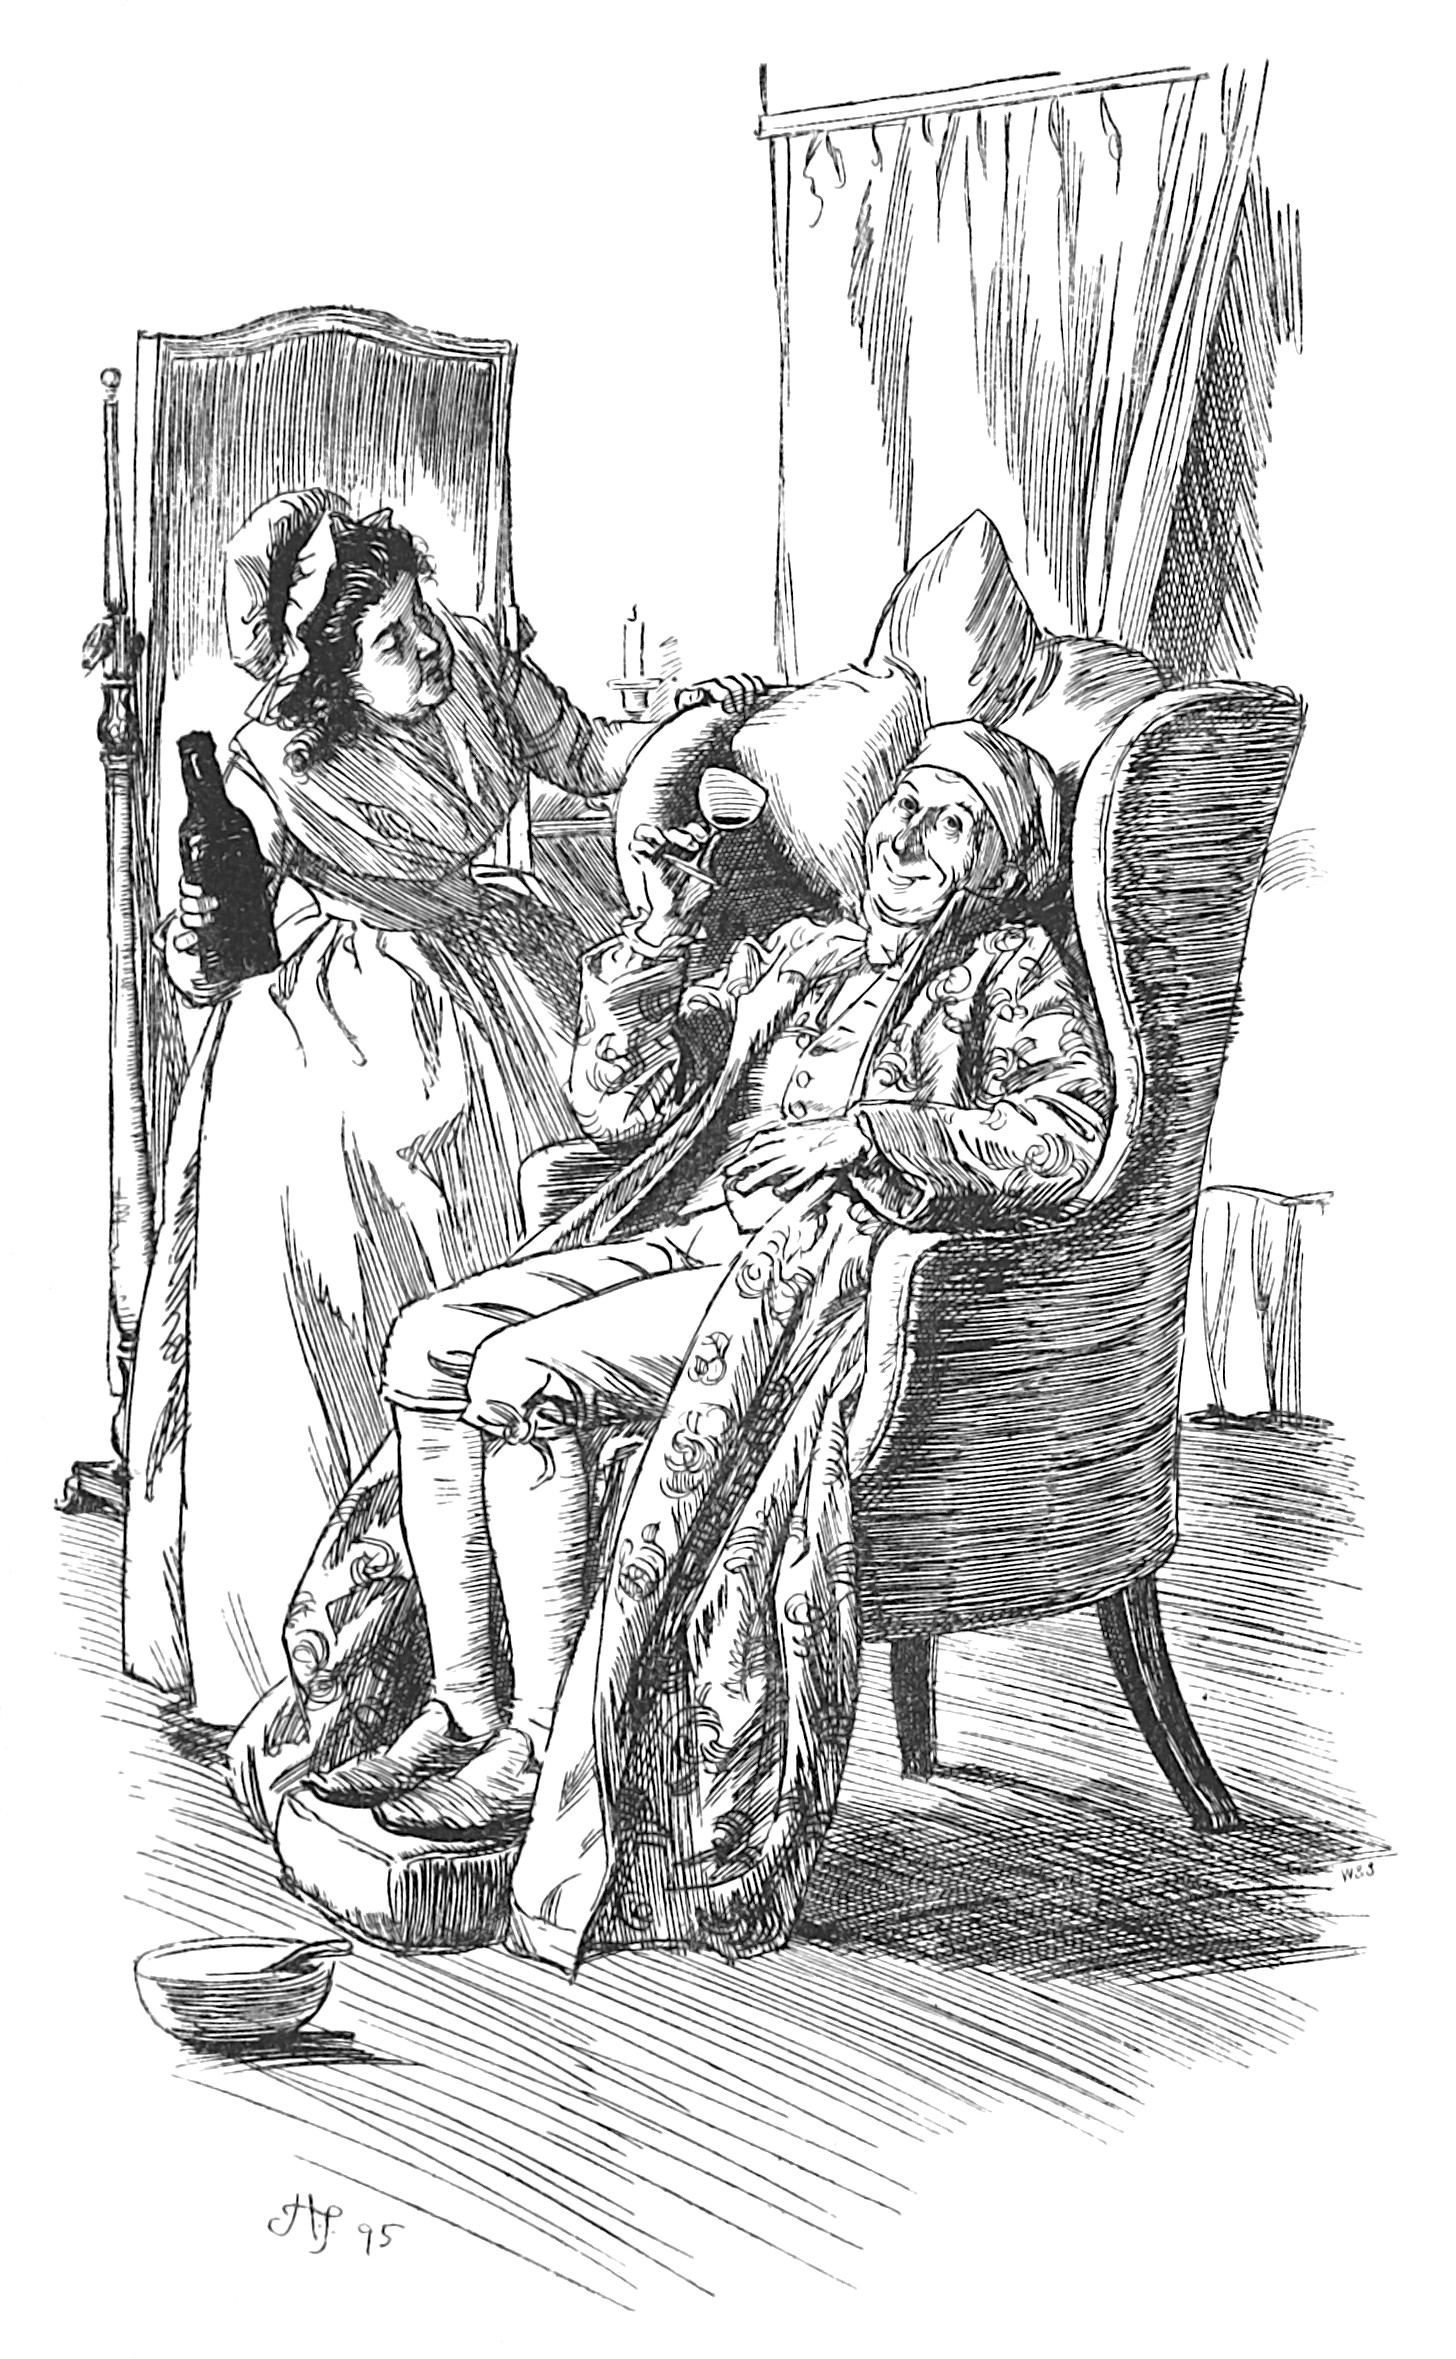
\includegraphics[width=.8\linewidth]{30fond}
		\caption{How fond he was of it!}
	\end{figure}
\end{a4}

\begin{letter}
	\begin{figure}[tbph]
		\centering
		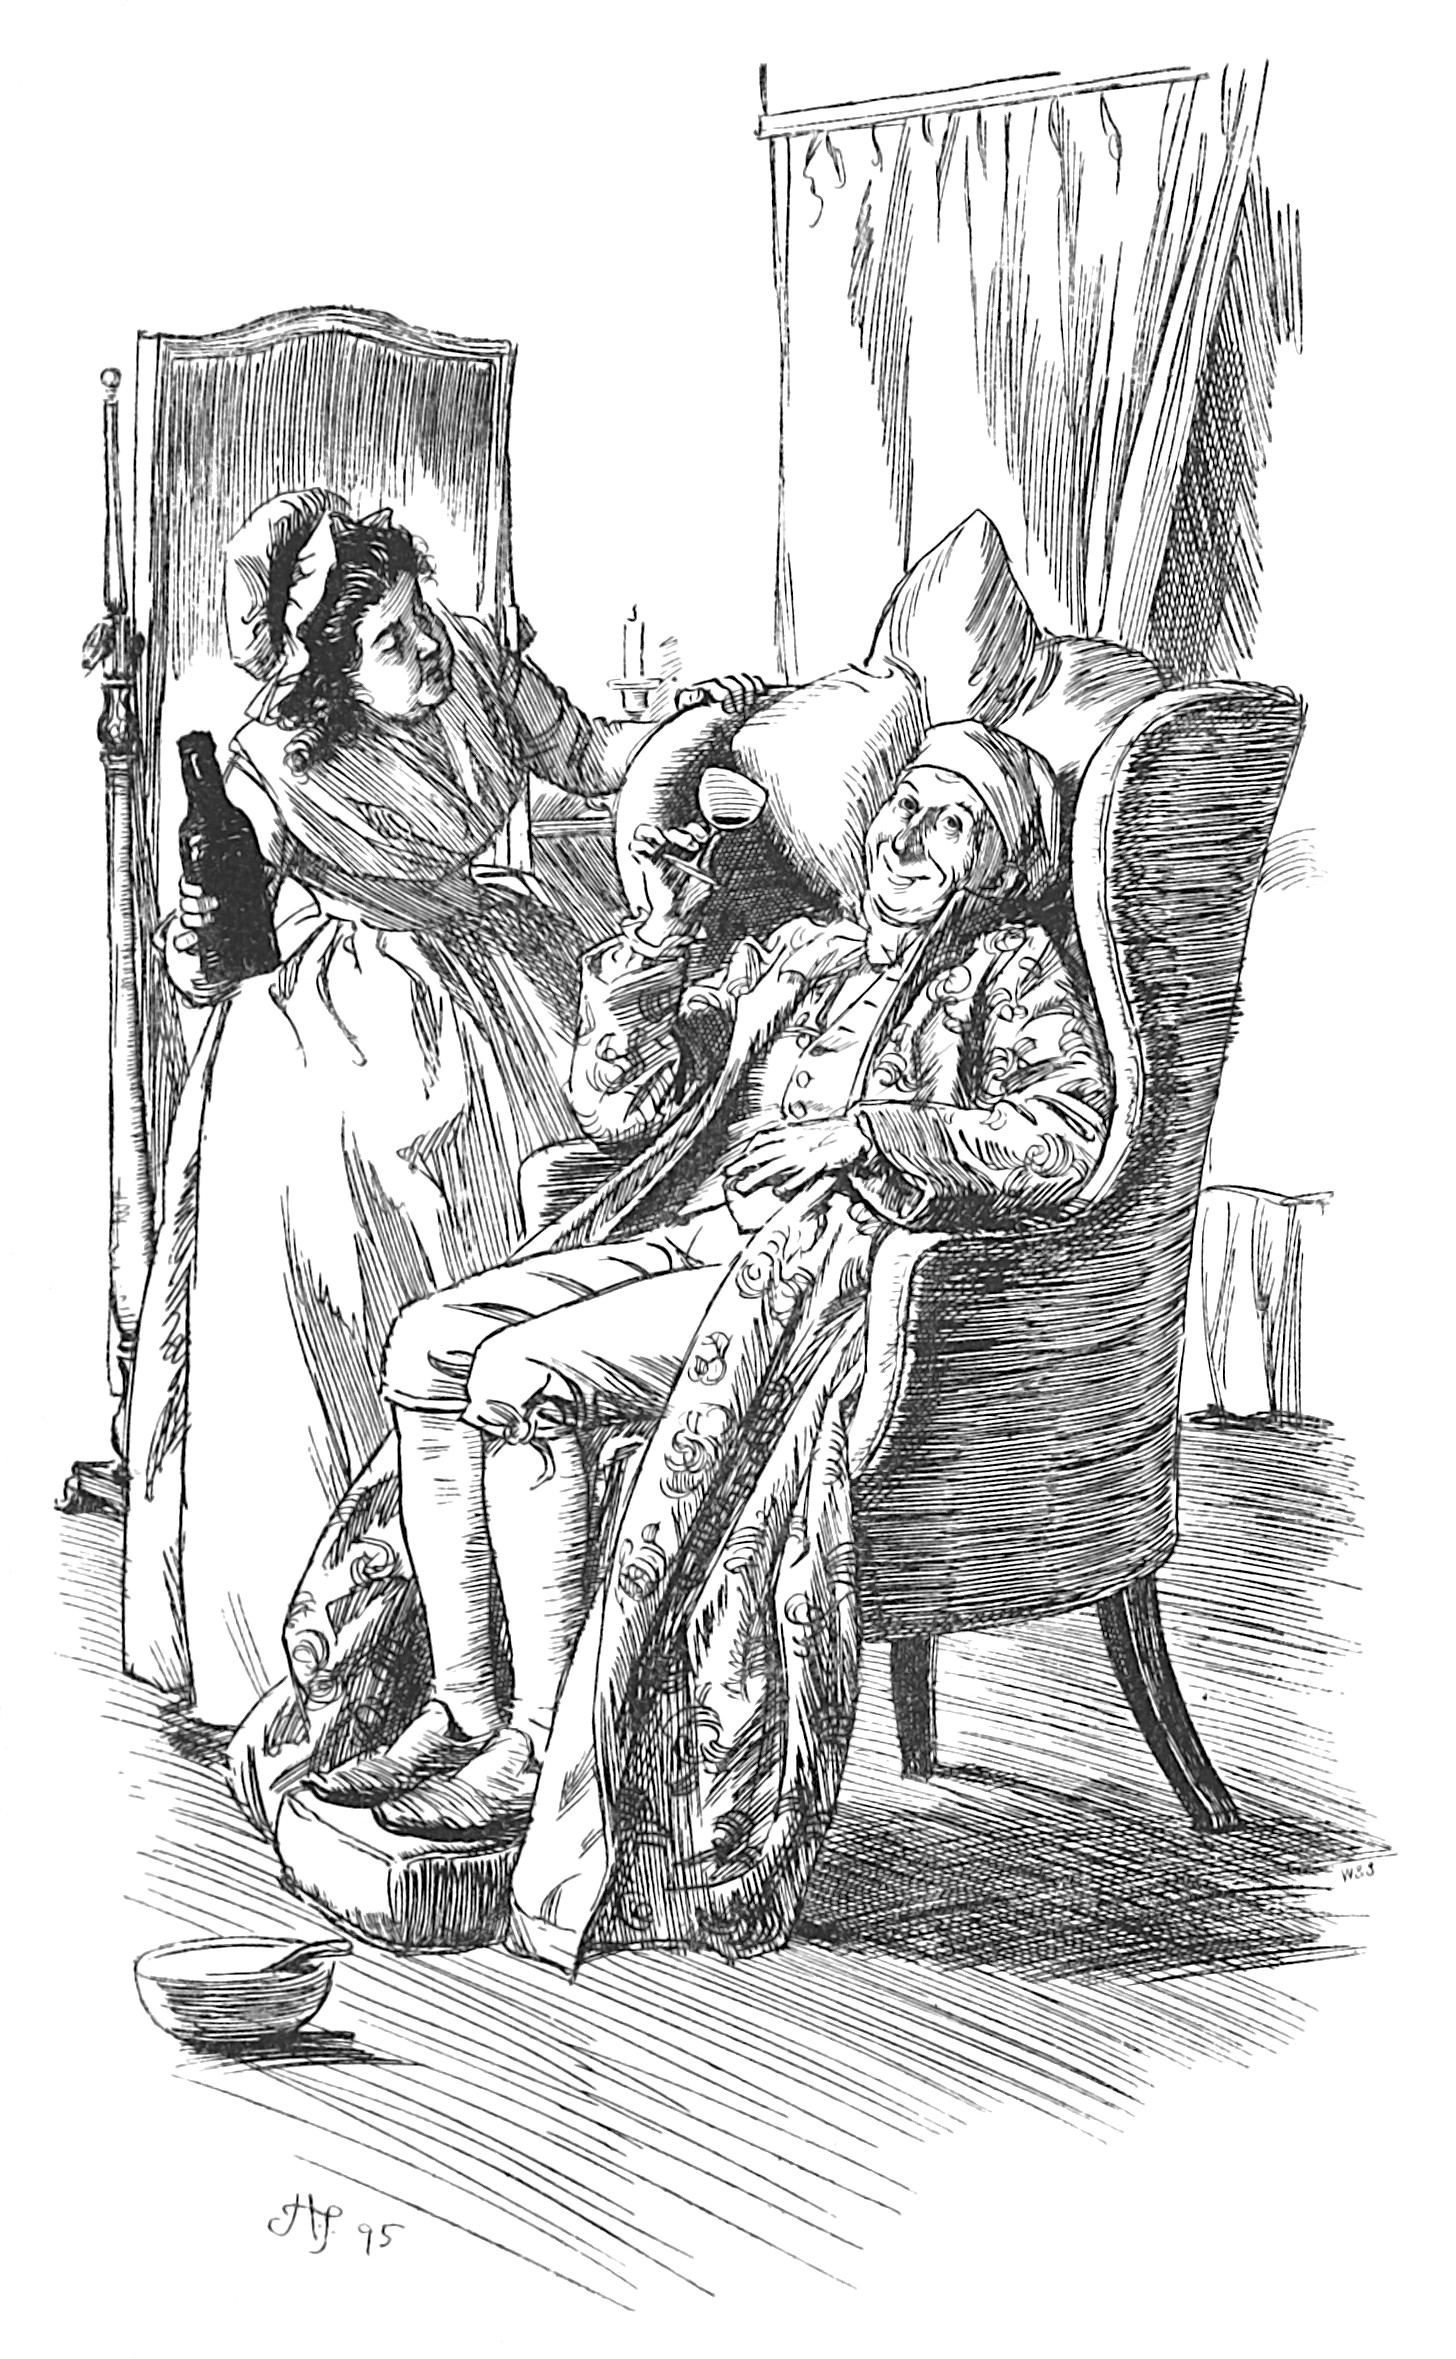
\includegraphics[width=\linewidth]{30fond}
		\caption{How fond he was of it!}
	\end{figure}
\end{letter}



»Dear Ma’am,« replied Elinor, smiling at the difference of the complaints for which it was recommended, »how good you are! But I have just left Marianne in bed, and, I hope, almost asleep; and as I think nothing will be of so much service to her as rest, if you will give me leave, I will drink the wine myself.«

Mrs Jennings, though regretting that she had not been five minutes earlier, was satisfied with the compromise; and Elinor, as she swallowed the chief of it, reflected, that though its effects on a colicky gout were, at present, of little importance to her, its healing powers, on a disappointed heart might be as reasonably tried on herself as on her sister.

Colonel Brandon came in while the party were at tea, and by his manner of looking round the room for Marianne, Elinor immediately fancied that he neither expected nor wished to see her there, and, in short, that he was already aware of what occasioned her absence. Mrs Jennings was not struck by the same thought; for soon after his entrance, she walked across the room to the tea-table where Elinor presided, and whispered, »The Colonel looks as grave as ever you see. He knows nothing of it; do tell him, my dear.«

He shortly afterwards drew a chair close to hers, and, with a look which perfectly assured her of his good information, inquired after her sister.

»Marianne is not well,« said she. »She has been indisposed all day, and we have persuaded her to go to bed.«

»Perhaps, then,« he hesitatingly replied, »what I heard this morning may be—there may be more truth in it than I could believe possible at first.«

»What did you hear?«

»That a gentleman, whom I had reason to think—in short, that a man, whom I \textit{knew} to be engaged—but how shall I tell you? If you know it already, as surely you must, I may be spared.«

»You mean,« answered Elinor, with forced calmness, »Mr Willoughby’s marriage with Miss Grey. Yes, we \textit{do} know it all. This seems to have been a day of general elucidation, for this very morning first unfolded it to us. Mr Willoughby is unfathomable! Where did you hear it?«

»In a stationer’s shop in Pall Mall, where I had business. Two ladies were waiting for their carriage, and one of them was giving the other an account of the intended match, in a voice so little attempting concealment, that it was impossible for me not to hear all. The name of Willoughby, John Willoughby, frequently repeated, first caught my attention; and what followed was a positive assertion that every thing was now finally settled respecting his marriage with Miss Grey—it was no longer to be a secret—it would take place even within a few weeks, with many particulars of preparations and other matters. One thing, especially, I remember, because it served to identify the man still more:—as soon as the ceremony was over, they were to go to Combe Magna, his seat in Somersetshire. My astonishment!—but it would be impossible to describe what I felt. The communicative lady I learnt, on inquiry, for I stayed in the shop till they were gone, was a Mrs Ellison, and that, as I have been since informed, is the name of Miss Grey’s guardian.«

»It is. But have you likewise heard that Miss Grey has fifty thousand pounds? In that, if in any thing, we may find an explanation.«

»It may be so; but Willoughby is capable—at least I think«—he stopped a moment; then added in a voice which seemed to distrust itself, »And your sister—how did she\longdash«

»Her sufferings have been very severe. I have only to hope that they may be proportionately short. It has been, it is a most cruel affliction. Till yesterday, I believe, she never doubted his regard; and even now, perhaps—but \textit{I} am almost convinced that he never was really attached to her. He has been very deceitful! and, in some points, there seems a hardness of heart about him.«

»Ah!« said Colonel Brandon, »there is, indeed! But your sister does not—I think you said so—she does not consider quite as you do?«

»You know her disposition, and may believe how eagerly she would still justify him if she could.«

He made no answer; and soon afterwards, by the removal of the tea-things, and the arrangement of the card parties, the subject was necessarily dropped. Mrs Jennings, who had watched them with pleasure while they were talking, and who expected to see the effect of Miss Dashwood’s communication, in such an instantaneous gaiety on Colonel Brandon’s side, as might have become a man in the bloom of youth, of hope and happiness, saw him, with amazement, remain the whole evening more serious and thoughtful than usual.
\chapter[Chapter \thechapter]{} 

 \lettrine{M}{r} and Mrs~Morland's surprise on being applied to by Mr~Tilney for their consent to his marrying their daughter was, for a few minutes, considerable, it having never entered their heads to suspect an attachment on either side; but as nothing, after all, could be more natural than Catherine's being beloved, they soon learnt to consider it with only the happy agitation of gratified pride, and, as far as they alone were concerned, had not a single objection to start. His pleasing manners and good sense were self-evident recommendations; and having never heard evil of him, it was not their way to suppose any evil could be told. Goodwill supplying the place of experience, his character needed no attestation. <Catherine would make a sad, heedless young housekeeper to be sure,> was her mother's foreboding remark; but quick was the consolation of there being nothing like practice. 

 There was but one obstacle, in short, to be mentioned; but till that one was removed, it must be impossible for them to sanction the engagement. Their tempers were mild, but their principles were steady, and while his parent so expressly forbade the connection, they could not allow themselves to encourage it. That the general should come forward to solicit the alliance, or that he should even very heartily approve it, they were not refined enough to make any parading stipulation; but the decent appearance of consent must be yielded, and that once obtained—and their own hearts made them trust that it could not be very long denied—their willing approbation was instantly to follow. His \textit{consent} was all that they wished for. They were no more inclined than entitled to demand his \textit{money}. Of a very considerable fortune, his son was, by marriage settlements, eventually secure; his present income was an income of independence and comfort, and under every pecuniary view, it was a match beyond the claims of their daughter. 

 The young people could not be surprised at a decision like this. They felt and they deplored—but they could not resent it; and they parted, endeavouring to hope that such a change in the general, as each believed almost impossible, might speedily take place, to unite them again in the fulness of privileged affection. Henry returned to what was now his only home, to watch over his young plantations, and extend his improvements for her sake, to whose share in them he looked anxiously forward; and Catherine remained at Fullerton to cry. Whether the torments of absence were softened by a clandestine correspondence, let us not inquire. Mr~and Mrs~Morland never did—they had been too kind to exact any promise; and whenever Catherine received a letter, as, at that time, happened pretty often, they always looked another way. 

 The anxiety, which in this state of their attachment must be the portion of Henry and Catherine, and of all who loved either, as to its final event, can hardly extend, I fear, to the bosom of my readers, who will see in the tell-tale compression of the pages before them, that we are all hastening together to perfect felicity. The means by which their early marriage was effected can be the only doubt: what probable circumstance could work upon a temper like the General's? The circumstance which chiefly availed was the marriage of his daughter with a man of fortune and consequence, which took place in the course of the summer—an accession of dignity that threw him into a fit of good humour, from which he did not recover till after Eleanor had obtained his forgiveness of Henry, and his permission for him <to be a fool if he liked it!> 

 The marriage of Eleanor Tilney, her removal from all the evils of such a home as Northanger had been made by Henry's banishment, to the home of her choice and the man of her choice, is an event which I expect to give general satisfaction among all her acquaintance. My own joy on the occasion is very sincere. I know no one more entitled, by unpretending merit, or better prepared by habitual suffering, to receive and enjoy felicity. Her partiality for this gentleman was not of recent origin; and he had been long withheld only by inferiority of situation from addressing her. His unexpected accession to title and fortune had removed all his difficulties; and never had the general loved his daughter so well in all her hours of companionship, utility, and patient endurance as when he first hailed her <Your Ladyship!> Her husband was really deserving of her; independent of his peerage, his wealth, and his attachment, being to a precision the most charming young man in the world. Any further definition of his merits must be unnecessary; the most charming young man in the world is instantly before the imagination of us all. Concerning the one in question, therefore, I have only to add—aware that the rules of composition forbid the introduction of a character not connected with my fable—that this was the very gentleman whose negligent servant left behind him that collection of washing-bills, resulting from a long visit at Northanger, by which my heroine was involved in one of her most alarming adventures. 

 The influence of the Viscount and Viscountess in their brother's behalf was assisted by that right understanding of Mr~Morland's circumstances which, as soon as the general would allow himself to be informed, they were qualified to give. It taught him that he had been scarcely more misled by Thorpe's first boast of the family wealth than by his subsequent malicious overthrow of it; that in no sense of the word were they necessitous or poor, and that Catherine would have three thousand pounds. This was so material an amendment of his late expectations that it greatly contributed to smooth the descent of his pride; and by no means without its effect was the private intelligence, which he was at some pains to procure, that the Fullerton estate, being entirely at the disposal of its present proprietor, was consequently open to every greedy speculation. 

 On the strength of this, the general, soon after Eleanor's marriage, permitted his son to return to Northanger, and thence made him the bearer of his consent, very courteously worded in a page full of empty professions to Mr~Morland. The event which it authorized soon followed: Henry and Catherine were married, the bells rang, and everybody smiled; and, as this took place within a twelvemonth from the first day of their meeting, it will not appear, after all the dreadful delays occasioned by the General's cruelty, that they were essentially hurt by it. To begin perfect happiness at the respective ages of twenty-six and eighteen is to do pretty well; and professing myself moreover convinced that the General's unjust interference, so far from being really injurious to their felicity, was perhaps rather conducive to it, by improving their knowledge of each other, and adding strength to their attachment, I leave it to be settled, by whomsoever it may concern, whether the tendency of this work be altogether to recommend parental tyranny, or reward filial disobedience. 
\chapter{Mrs~Johnson to Lady~Susan}
  
  	\begin{a4}
	\vspace{5em}
	\end{a4}
	
  \begin{mail}{Edward Street.}{My dear Creature,}
 
 I am in agonies, and know not what to do. Mr~De Courcy arrived just when he should not. Mrs~Mainwaring had that instant entered the house, and forced herself into her guardian's presence, though I did not know a syllable of it till afterwards, for I was out when both she and Reginald came, or I should have sent him away at all events; but she was shut up with Mr~Johnson, while he waited in the drawing-room for me. She arrived yesterday in pursuit of her husband, but perhaps you know this already from himself. She came to this house to entreat my husband's interference, and before I could be aware of it, everything that you could wish to be concealed was known to him, and unluckily she had wormed out of Mainwaring's servant that he had visited you every day since your being in town, and had just watched him to your door herself! What could I do! Facts are such horrid things! All is by this time known to De Courcy, who is now alone with Mr~Johnson. Do not accuse me; indeed, it was impossible to prevent it. Mr~Johnson has for some time suspected De Courcy of intending to marry you, and would speak with him alone as soon as he knew him to be in the house. That detestable Mrs~Mainwaring, who, for your comfort, has fretted herself thinner and uglier than ever, is still here, and they have been all closeted together. What can be done? At any rate, I hope he will plague his wife more than ever. With anxious wishes, 

\closeletter[Yours faithfully,]{Alicia.} 
\end{mail}
%!TeX root=../pridetop.tex
\chapter[Chapter \thechapter]{}
	
	\begin{figure}[t!]
\centering
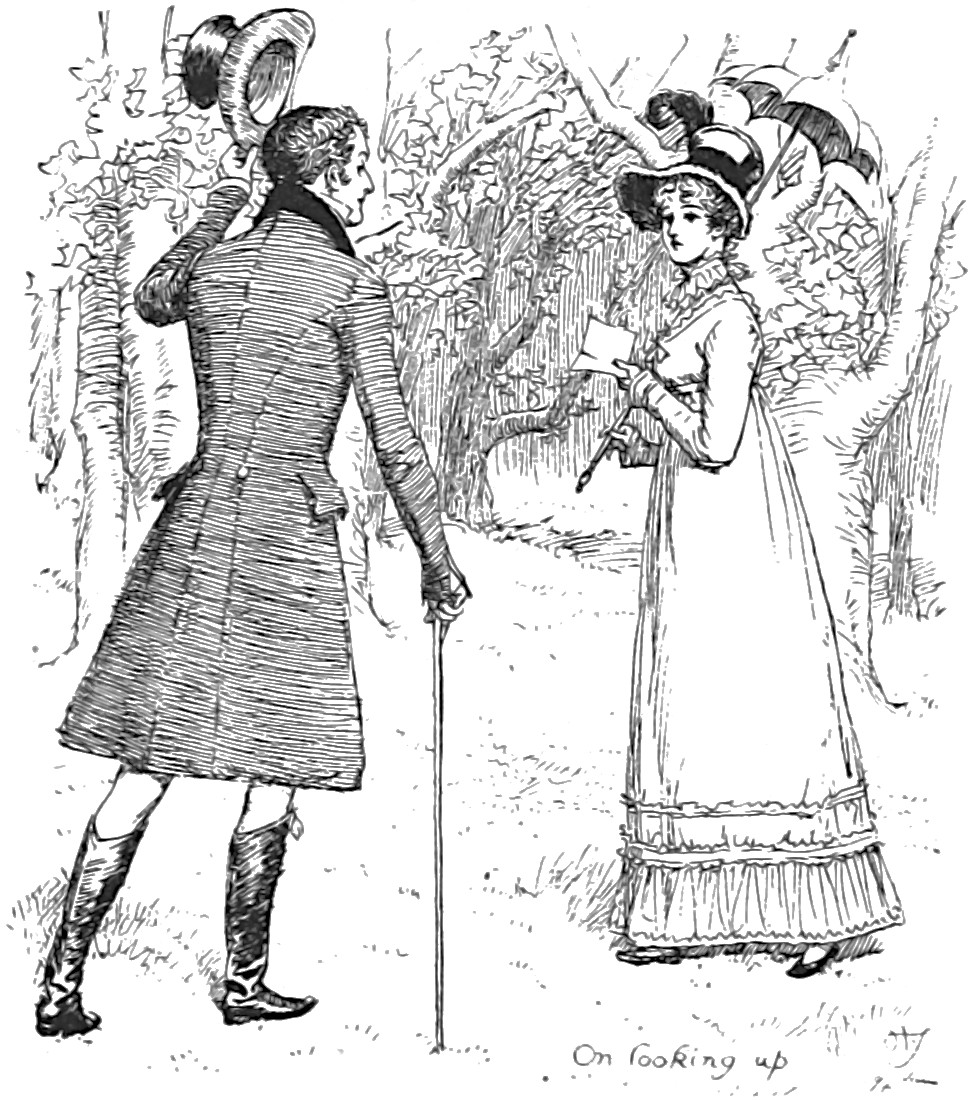
\includegraphics[width=.8\linewidth]{33top}
\captionlistentry{Headpiece to Chapter \thechapter}
\end{figure}


\lettrine[lines=6,image=true]{initials/chap33m}{ore}  than once did Elizabeth, in her ramble within the park, unexpectedly meet Mr Darcy. She felt all the perverseness of the mischance that should bring him where no one else was brought; and, to prevent its ever happening again, took care to inform him, at first, that it was a favourite haunt of hers. How it could occur a second time, therefore, was very odd! Yet it did, and even the third. It seemed like wilful ill-nature, or a voluntary penance; for on these occasions it was not merely a few formal inquiries and an awkward pause and then away, but he actually thought it necessary to turn back and walk with her. He never said a great deal, nor did she give herself the trouble of talking or of listening much; but it struck her in the course of their third rencounter that he was asking some odd unconnected questions—about her pleasure in being at Hunsford, her love of solitary walks, and her opinion of Mr and Mrs Collins's happiness; and that in speaking of Rosings, and her not perfectly understanding the house, he seemed to expect that whenever she came into Kent again she would be staying \textit{there} too. His words seemed to imply it. Could he have Colonel Fitzwilliam in his thoughts? She supposed, if he meant anything, he must mean an allusion to what might arise in that quarter. It distressed her a little, and she was quite glad to find herself at the gate in the pales opposite the Parsonage.

She was engaged one day, as she walked, in re-perusing Jane's last letter, and dwelling on some passages which proved that Jane had not written in spirits, when, instead of being again surprised by Mr Darcy, she saw, on looking up, that Colonel Fitzwilliam was meeting her. Putting away the letter immediately, and forcing a smile, she said,—

<I did not know before that you ever walked this way.>

<I have been making the tour of the park,> he replied, <as I generally do every year, and intended to close it with a call at the Parsonage. Are you going much farther?>

<No, I should have turned in a moment.>

And accordingly she did turn, and they walked towards the Parsonage together.

<Do you certainly leave Kent on Saturday?> said she.

<Yes—if Darcy does not put it off again. But I am at his disposal. He arranges the business just as he pleases.>

<And if not able to please himself in the arrangement, he has at least great pleasure in the power of choice. I do not know anybody who seems more to enjoy the power of doing what he likes than Mr Darcy.>

<He likes to have his own way very well,> replied Colonel Fitzwilliam. <But so we all do. It is only that he has better means of having it than many others, because he is rich, and many others are poor. I speak feelingly. A younger son, you know, must be inured to self-denial and dependence.>

<In my opinion, the younger son of an earl can know very little of either. Now, seriously, what have you ever known of self-denial and dependence? When have you been prevented by want of money from going wherever you chose or procuring anything you had a fancy for?>

<These are home questions—and perhaps I cannot say that I have experienced many hardships of that nature. But in matters of greater weight, I may suffer from the want of money. Younger sons cannot marry where they like.>

<Unless where they like women of fortune, which I think they very often do.>

<Our habits of expense make us too dependent, and there are not many in my rank of life who can afford to marry without some attention to money.>

<Is this,> thought Elizabeth, <meant for me?> and she coloured at the idea; but, recovering herself, said in a lively tone, <And pray, what is the usual price of an earl's younger son? Unless the elder brother is very sickly, I suppose you would not ask above fifty thousand pounds.>

He answered her in the same style, and the subject dropped. To interrupt a silence which might make him fancy her affected with what had passed, she soon afterwards said,—

<I imagine your cousin brought you down with him chiefly for the sake of having somebody at his disposal. I wonder he does not marry, to secure a lasting convenience of that kind. But, perhaps, his sister does as well for the present; and, as she is under his sole care, he may do what he likes with her.>

<No,> said Colonel Fitzwilliam, <that is an advantage which he must divide with me. I am joined with him in the guardianship of Miss Darcy.>

<Are you, indeed? And pray what sort of a guardian do you make? Does your charge give you much trouble? Young ladies of her age are sometimes a little difficult to manage; and if she has the true Darcy spirit, she may like to have her own way.>

As she spoke, she observed him looking at her earnestly; and the manner in which he immediately asked her why she supposed Miss Darcy likely to give them any uneasiness, convinced her that she had somehow or other got pretty near the truth. She directly replied,—

<You need not be frightened. I never heard any harm of her; and I dare say she is one of the most tractable creatures in the world. She is a very great favourite with some ladies of my acquaintance, Mrs Hurst and Miss Bingley. I think I have heard you say that you know them.>

<I know them a little. Their brother is a pleasant, gentlemanlike man—he is a great friend of Darcy's.>

<Oh yes,> said Elizabeth drily—<Mr Darcy is uncommonly kind to Mr Bingley, and takes a prodigious deal of care of him.>

<Care of him! Yes, I really believe Darcy \textit{does} take care of him in those points where he most wants care. From something that he told me in our journey hither, I have reason to think Bingley very much indebted to him. But I ought to beg his pardon, for I have no right to suppose that Bingley was the person meant. It was all conjecture.>

<What is it you mean?>

<It is a circumstance which Darcy of course could not wish to be generally known, because if it were to get round to the lady's family it would be an unpleasant thing.>

<You may depend upon my not mentioning it.>

<And remember that I have not much reason for supposing it to be Bingley. What he told me was merely this: that he congratulated himself on having lately saved a friend from the inconveniences of a most imprudent marriage, but without mentioning names or any other particulars; and I only suspected it to be Bingley from believing him the kind of young man to get into a scrape of that sort, and from knowing them to have been together the whole of last summer.>

<Did Mr Darcy give you his reasons for this interference?>

<I understood that there were some very strong objections against the lady.>

<And what arts did he use to separate them?>

<He did not talk to me of his own arts,> said Fitzwilliam, smiling. <He only told me what I have now told you.>

Elizabeth made no answer, and walked on, her heart swelling with indignation. After watching her a little, Fitzwilliam asked her why she was so thoughtful.

<I am thinking of what you have been telling me,> said she. <Your cousin's conduct does not suit my feelings. Why was he to be the judge?>

<You are rather disposed to call his interference officious?>

<I do not see what right Mr Darcy had to decide on the propriety of his friend's inclination; or why, upon his own judgment alone, he was to determine and direct in what manner that friend was to be happy. But,> she continued, recollecting herself, <as we know none of the particulars, it is not fair to condemn him. It is not to be supposed that there was much affection in the case.>

<That is not an unnatural surmise,> said Fitzwilliam; <but it is lessening the honour of my cousin's triumph very sadly.>

This was spoken jestingly, but it appeared to her so just a picture of Mr Darcy, that she would not trust herself with an answer; and, therefore, abruptly changing the conversation, talked on indifferent matters till they reached the Parsonage. There, shut into her own room, as soon as their visitor left them, she could think without interruption of all that she had heard. It was not to be supposed that any other people could be meant than those with whom she was connected. There could not exist in the world \textit{two} men over whom Mr Darcy could have such boundless influence. That he had been concerned in the measures taken to separate Mr Bingley and Jane, she had never doubted; but she had always attributed to Miss Bingley the principal design and arrangement of them. If his own vanity, however, did not mislead him, \textit{he} was the cause—his pride and caprice were the cause—of all that Jane had suffered, and still continued to suffer. He had ruined for a while every hope of happiness for the most affectionate, generous heart in the world; and no one could say how lasting an evil he might have inflicted.

<There were some very strong objections against the lady,> were Colonel Fitzwilliam's words; and these strong objections probably were, her having one uncle who was a country attorney, and another who was in business in London.

<To Jane herself,> she exclaimed, <there could be no possibility of objection,—all loveliness and goodness as she is! Her understanding excellent, her mind improved, and her manners captivating. Neither could anything be urged against my father, who, though with some peculiarities, has abilities which Mr Darcy himself need not disdain, and respectability which he will probably never reach.> When she thought of her mother, indeed, her confidence gave way a little; but she would not allow that any objections \textit{there} had material weight with Mr Darcy, whose pride, she was convinced, would receive a deeper wound from the want of importance in his friend's connections than from their want of sense; and she was quite decided, at last, that he had been partly governed by this worst kind of pride, and partly by the wish of retaining Mr Bingley for his sister.

The agitation and tears which the subject occasioned brought on a headache; and it grew so much worse towards the evening that, added to her unwillingness to see Mr Darcy, it determined her not to attend her cousins to Rosings, where they were engaged to drink tea. Mrs Collins, seeing that she was really unwell, did not press her to go, and as much as possible prevented her husband from pressing her; but Mr Collins could not conceal his apprehension of Lady Catherine's being rather displeased by her staying at home.

\chapter[Chapter \thechapter]{} 

 \lettrine[lraise=0.3]{E}{dmund} had great things to hear on his return. Many surprises were awaiting him. The first that occurred was not least in interest: the appearance of Henry Crawford and his sister walking together through the village as he rode into it. He had concluded—he had meant them to be far distant. His absence had been extended beyond a fortnight purposely to avoid Miss~Crawford. He was returning to Mansfield with spirits ready to feed on melancholy remembrances, and tender associations, when her own fair self was before him, leaning on her brother's arm, and he found himself receiving a welcome, unquestionably friendly, from the woman whom, two moments before, he had been thinking of as seventy miles off, and as farther, much farther, from him in inclination than any distance could express.

Her reception of him was of a sort which he could not have hoped for, had he expected to see her. Coming as he did from such a purport fulfilled as had taken him away, he would have expected anything rather than a look of satisfaction, and words of simple, pleasant meaning. It was enough to set his heart in a glow, and to bring him home in the properest state for feeling the full value of the other joyful surprises at hand.

William's promotion, with all its particulars, he was soon master of; and with such a secret provision of comfort within his own breast to help the joy, he found in it a source of most gratifying sensation and unvarying cheerfulness all dinner-time.

After dinner, when he and his father were alone, he had Fanny's history; and then all the great events of the last fortnight, and the present situation of matters at Mansfield were known to him.

Fanny suspected what was going on. They sat so much longer than usual in the dining-parlour, that she was sure they must be talking of her; and when tea at last brought them away, and she was to be seen by Edmund again, she felt dreadfully guilty. He came to her, sat down by her, took her hand, and pressed it kindly; and at that moment she thought that, but for the occupation and the scene which the tea-things afforded, she must have betrayed her emotion in some unpardonable excess.

He was not intending, however, by such action, to be conveying to her that unqualified approbation and encouragement which her hopes drew from it. It was designed only to express his participation in all that interested her, and to tell her that he had been hearing what quickened every feeling of affection. He was, in fact, entirely on his father's side of the question. His surprise was not so great as his father's at her refusing Crawford, because, so far from supposing her to consider him with anything like a preference, he had always believed it to be rather the reverse, and could imagine her to be taken perfectly unprepared, but Sir~Thomas could not regard the connexion as more desirable than he did. It had every recommendation to him; and while honouring her for what she had done under the influence of her present indifference, honouring her in rather stronger terms than Sir~Thomas could quite echo, he was most earnest in hoping, and sanguine in believing, that it would be a match at last, and that, united by mutual affection, it would appear that their dispositions were as exactly fitted to make them blessed in each other, as he was now beginning seriously to consider them. Crawford had been too precipitate. He had not given her time to attach herself. He had begun at the wrong end. With such powers as his, however, and such a disposition as hers, Edmund trusted that everything would work out a happy conclusion. Meanwhile, he saw enough of Fanny's embarrassment to make him scrupulously guard against exciting it a second time, by any word, or look, or movement.

Crawford called the next day, and on the score of Edmund's return, Sir~Thomas felt himself more than licensed to ask him to stay dinner; it was really a necessary compliment. He staid of course, and Edmund had then ample opportunity for observing how he sped with Fanny, and what degree of immediate encouragement for him might be extracted from her manners; and it was so little, so very, very little—every chance, every possibility of it, resting upon her embarrassment only; if there was not hope in her confusion, there was hope in nothing else—that he was almost ready to wonder at his friend's perseverance. Fanny was worth it all; he held her to be worth every effort of patience, every exertion of mind, but he did not think he could have gone on himself with any woman breathing, without something more to warm his courage than his eyes could discern in hers. He was very willing to hope that Crawford saw clearer, and this was the most comfortable conclusion for his friend that he could come to from all that he observed to pass before, and at, and after dinner.

In the evening a few circumstances occurred which he thought more promising. When he and Crawford walked into the drawing-room, his mother and Fanny were sitting as intently and silently at work as if there were nothing else to care for. Edmund could not help noticing their apparently deep tranquillity.

<We have not been so silent all the time,> replied his mother. <Fanny has been reading to me, and only put the book down upon hearing you coming.> And sure enough there was a book on the table which had the air of being very recently closed: a volume of Shakespeare. <She often reads to me out of those books; and she was in the middle of a very fine speech of that man's—what's his name, Fanny?—when we heard your footsteps.>

Crawford took the volume. <Let me have the pleasure of finishing that speech to your ladyship,> said he. <I shall find it immediately.> And by carefully giving way to the inclination of the leaves, he did find it, or within a page or two, quite near enough to satisfy Lady Bertram, who assured him, as soon as he mentioned the name of Cardinal Wolsey, that he had got the very speech. Not a look or an offer of help had Fanny given; not a syllable for or against. All her attention was for her work. She seemed determined to be interested by nothing else. But taste was too strong in her. She could not abstract her mind five minutes: she was forced to listen; his reading was capital, and her pleasure in good reading extreme. To \textit{good}  reading, however, she had been long used: her uncle read well, her cousins all, Edmund very well, but in Mr~Crawford's reading there was a variety of excellence beyond what she had ever met with. The King, the Queen, Buckingham, Wolsey, Cromwell, all were given in turn; for with the happiest knack, the happiest power of jumping and guessing, he could always alight at will on the best scene, or the best speeches of each; and whether it were dignity, or pride, or tenderness, or remorse, or whatever were to be expressed, he could do it with equal beauty. It was truly dramatic. His acting had first taught Fanny what pleasure a play might give, and his reading brought all his acting before her again; nay, perhaps with greater enjoyment, for it came unexpectedly, and with no such drawback as she had been used to suffer in seeing him on the stage with Miss~Bertram.

Edmund watched the progress of her attention, and was amused and gratified by seeing how she gradually slackened in the needlework, which at the beginning seemed to occupy her totally: how it fell from her hand while she sat motionless over it, and at last, how the eyes which had appeared so studiously to avoid him throughout the day were turned and fixed on Crawford—fixed on him for minutes, fixed on him, in short, till the attraction drew Crawford's upon her, and the book was closed, and the charm was broken. Then she was shrinking again into herself, and blushing and working as hard as ever; but it had been enough to give Edmund encouragement for his friend, and as he cordially thanked him, he hoped to be expressing Fanny's secret feelings too.

<That play must be a favourite with you,> said he; <you read as if you knew it well.>

<It will be a favourite, I believe, from this hour,> replied Crawford; <but I do not think I have had a volume of Shakespeare in my hand before since I was fifteen. I once saw Henry the Eighth acted, or I have heard of it from somebody who did, I am not certain which. But Shakespeare one gets acquainted with without knowing how. It is a part of an Englishman's constitution. His thoughts and beauties are so spread abroad that one touches them everywhere; one is intimate with him by instinct. No man of any brain can open at a good part of one of his plays without falling into the flow of his meaning immediately.>

<No doubt one is familiar with Shakespeare in a degree,> said Edmund, <from one's earliest years. His celebrated passages are quoted by everybody; they are in half the books we open, and we all talk Shakespeare, use his similes, and describe with his descriptions; but this is totally distinct from giving his sense as you gave it. To know him in bits and scraps is common enough; to know him pretty thoroughly is, perhaps, not uncommon; but to read him well aloud is no everyday talent.>

<Sir, you do me honour,> was Crawford's answer, with a bow of mock gravity.

Both gentlemen had a glance at Fanny, to see if a word of accordant praise could be extorted from her; yet both feeling that it could not be. Her praise had been given in her attention; \textit{that}  must content them.

Lady Bertram's admiration was expressed, and strongly too. <It was really like being at a play,> said she. <I wish Sir~Thomas had been here.>

Crawford was excessively pleased. If Lady Bertram, with all her incompetency and languor, could feel this, the inference of what her niece, alive and enlightened as she was, must feel, was elevating.

<You have a great turn for acting, I am sure, Mr~Crawford,> said her ladyship soon afterwards; <and I will tell you what, I think you will have a theatre, some time or other, at your house in Norfolk. I mean when you are settled there. I do indeed. I think you will fit up a theatre at your house in Norfolk.>

<Do you, ma'am?> cried he, with quickness. <No, no, that will never be. Your ladyship is quite mistaken. No theatre at Everingham! Oh no!> And he looked at Fanny with an expressive smile, which evidently meant, <That lady will never allow a theatre at Everingham.>

Edmund saw it all, and saw Fanny so determined \textit{not}  to see it, as to make it clear that the voice was enough to convey the full meaning of the protestation; and such a quick consciousness of compliment, such a ready comprehension of a hint, he thought, was rather favourable than not.

The subject of reading aloud was farther discussed. The two young men were the only talkers, but they, standing by the fire, talked over the too common neglect of the qualification, the total inattention to it, in the ordinary school-system for boys, the consequently natural, yet in some instances almost unnatural, degree of ignorance and uncouthness of men, of sensible and well-informed men, when suddenly called to the necessity of reading aloud, which had fallen within their notice, giving instances of blunders, and failures with their secondary causes, the want of management of the voice, of proper modulation and emphasis, of foresight and judgment, all proceeding from the first cause: want of early attention and habit; and Fanny was listening again with great entertainment.

<Even in my profession,> said Edmund, with a smile, <how little the art of reading has been studied! how little a clear manner, and good delivery, have been attended to! I speak rather of the past, however, than the present. There is now a spirit of improvement abroad; but among those who were ordained twenty, thirty, forty years ago, the larger number, to judge by their performance, must have thought reading was reading, and preaching was preaching. It is different now. The subject is more justly considered. It is felt that distinctness and energy may have weight in recommending the most solid truths; and besides, there is more general observation and taste, a more critical knowledge diffused than formerly; in every congregation there is a larger proportion who know a little of the matter, and who can judge and criticise.>

Edmund had already gone through the service once since his ordination; and upon this being understood, he had a variety of questions from Crawford as to his feelings and success; questions, which being made, though with the vivacity of friendly interest and quick taste, without any touch of that spirit of banter or air of levity which Edmund knew to be most offensive to Fanny, he had true pleasure in satisfying; and when Crawford proceeded to ask his opinion and give his own as to the properest manner in which particular passages in the service should be delivered, shewing it to be a subject on which he had thought before, and thought with judgment, Edmund was still more and more pleased. This would be the way to Fanny's heart. She was not to be won by all that gallantry and wit and good-nature together could do; or, at least, she would not be won by them nearly so soon, without the assistance of sentiment and feeling, and seriousness on serious subjects.

<Our liturgy,> observed Crawford, <has beauties, which not even a careless, slovenly style of reading can destroy; but it has also redundancies and repetitions which require good reading not to be felt. For myself, at least, I must confess being not always so attentive as I ought to be> (here was a glance at Fanny); <that nineteen times out of twenty I am thinking how such a prayer ought to be read, and longing to have it to read myself. Did you speak?> stepping eagerly to Fanny, and addressing her in a softened voice; and upon her saying <No,> he added, <Are you sure you did not speak? I saw your lips move. I fancied you might be going to tell me I ought to be more attentive, and not \textit{allow}  my thoughts to wander. Are not you going to tell me so?>

<No, indeed, you know your duty too well for me to—even supposing\longdash>

She stopt, felt herself getting into a puzzle, and could not be prevailed on to add another word, not by dint of several minutes of supplication and waiting. He then returned to his former station, and went on as if there had been no such tender interruption.

<A sermon, well delivered, is more uncommon even than prayers well read. A sermon, good in itself, is no rare thing. It is more difficult to speak well than to compose well; that is, the rules and trick of composition are oftener an object of study. A thoroughly good sermon, thoroughly well delivered, is a capital gratification. I can never hear such a one without the greatest admiration and respect, and more than half a mind to take orders and preach myself. There is something in the eloquence of the pulpit, when it is really eloquence, which is entitled to the highest praise and honour. The preacher who can touch and affect such an heterogeneous mass of hearers, on subjects limited, and long worn threadbare in all common hands; who can say anything new or striking, anything that rouses the attention without offending the taste, or wearing out the feelings of his hearers, is a man whom one could not, in his public capacity, honour enough. I should like to be such a man.>

Edmund laughed.

<I should indeed. I never listened to a distinguished preacher in my life without a sort of envy. But then, I must have a London audience. I could not preach but to the educated; to those who were capable of estimating my composition. And I do not know that I should be fond of preaching often; now and then, perhaps once or twice in the spring, after being anxiously expected for half a dozen Sundays together; but not for a constancy; it would not do for a constancy.>

Here Fanny, who could not but listen, involuntarily shook her head, and Crawford was instantly by her side again, entreating to know her meaning; and as Edmund perceived, by his drawing in a chair, and sitting down close by her, that it was to be a very thorough attack, that looks and undertones were to be well tried, he sank as quietly as possible into a corner, turned his back, and took up a newspaper, very sincerely wishing that dear little Fanny might be persuaded into explaining away that shake of the head to the satisfaction of her ardent lover; and as earnestly trying to bury every sound of the business from himself in murmurs of his own, over the various advertisements of <A most desirable Estate in South Wales>; <To Parents and Guardians>; and a <Capital season'd Hunter.>

Fanny, meanwhile, vexed with herself for not having been as motionless as she was speechless, and grieved to the heart to see Edmund's arrangements, was trying by everything in the power of her modest, gentle nature, to repulse Mr~Crawford, and avoid both his looks and inquiries; and he, unrepulsable, was persisting in both.

<What did that shake of the head mean?> said he. <What was it meant to express? Disapprobation, I fear. But of what? What had I been saying to displease you? Did you think me speaking improperly, lightly, irreverently on the subject? Only tell me if I was. Only tell me if I was wrong. I want to be set right. Nay, nay, I entreat you; for one moment put down your work. What did that shake of the head mean?>

In vain was her <Pray, sir, don't; pray, Mr~Crawford,> repeated twice over; and in vain did she try to move away. In the same low, eager voice, and the same close neighbourhood, he went on, reurging the same questions as before. She grew more agitated and displeased.

<How can you, sir? You quite astonish me; I wonder how you can\longdash>

<Do I astonish you?> said he. <Do you wonder? Is there anything in my present entreaty that you do not understand? I will explain to you instantly all that makes me urge you in this manner, all that gives me an interest in what you look and do, and excites my present curiosity. I will not leave you to wonder long.>

In spite of herself, she could not help half a smile, but she said nothing.

<You shook your head at my acknowledging that I should not like to engage in the duties of a clergyman always for a constancy. Yes, that was the word. Constancy: I am not afraid of the word. I would spell it, read it, write it with anybody. I see nothing alarming in the word. Did you think I ought?>

<Perhaps, sir,> said Fanny, wearied at last into speaking—<perhaps, sir, I thought it was a pity you did not always know yourself as well as you seemed to do at that moment.>

Crawford, delighted to get her to speak at any rate, was determined to keep it up; and poor Fanny, who had hoped to silence him by such an extremity of reproof, found herself sadly mistaken, and that it was only a change from one object of curiosity and one set of words to another. He had always something to entreat the explanation of. The opportunity was too fair. None such had occurred since his seeing her in her uncle's room, none such might occur again before his leaving Mansfield. Lady Bertram's being just on the other side of the table was a trifle, for she might always be considered as only half-awake, and Edmund's advertisements were still of the first utility.

<Well,> said Crawford, after a course of rapid questions and reluctant answers; <I am happier than I was, because I now understand more clearly your opinion of me. You think me unsteady: easily swayed by the whim of the moment, easily tempted, easily put aside. With such an opinion, no wonder that—But we shall see.—It is not by protestations that I shall endeavour to convince you I am wronged; it is not by telling you that my affections are steady. My conduct shall speak for me; absence, distance, time shall speak for me. \textit{They}  shall prove that, as far as you can be deserved by anybody, I do deserve you. You are infinitely my superior in merit; all \textit{that}  I know. You have qualities which I had not before supposed to exist in such a degree in any human creature. You have some touches of the angel in you beyond what—not merely beyond what one sees, because one never sees anything like it—but beyond what one fancies might be. But still I am not frightened. It is not by equality of merit that you can be won. That is out of the question. It is he who sees and worships your merit the strongest, who loves you most devotedly, that has the best right to a return. There I build my confidence. By that right I do and will deserve you; and when once convinced that my attachment is what I declare it, I know you too well not to entertain the warmest hopes. Yes, dearest, sweetest Fanny. Nay> (seeing her draw back displeased), <forgive me. Perhaps I have as yet no right; but by what other name can I call you? Do you suppose you are ever present to my imagination under any other? No, it is <Fanny> that I think of all day, and dream of all night. You have given the name such reality of sweetness, that nothing else can now be descriptive of you.>

Fanny could hardly have kept her seat any longer, or have refrained from at least trying to get away in spite of all the too public opposition she foresaw to it, had it not been for the sound of approaching relief, the very sound which she had been long watching for, and long thinking strangely delayed.

The solemn procession, headed by Baddeley, of tea-board, urn, and cake-bearers, made its appearance, and delivered her from a grievous imprisonment of body and mind. Mr~Crawford was obliged to move. She was at liberty, she was busy, she was protected.

Edmund was not sorry to be admitted again among the number of those who might speak and hear. But though the conference had seemed full long to him, and though on looking at Fanny he saw rather a flush of vexation, he inclined to hope that so much could not have been said and listened to without some profit to the speaker. 
%!TeX root=../emmatop.tex
\chapter[Chapter \thechapter]{}
\lettrine[lraise=0.35]{W}{hen} the ladies returned to the drawing-room after dinner, Emma found it hardly possible to prevent their making two distinct parties;—with so much perseverance in judging and behaving ill did Mrs Elton engross Jane Fairfax and slight herself. She and Mrs Weston were obliged to be almost always either talking together or silent together. Mrs Elton left them no choice. If Jane repressed her for a little time, she soon began again; and though much that passed between them was in a half-whisper, especially on Mrs Elton's side, there was no avoiding a knowledge of their principal subjects: The post-office—catching cold—fetching letters—and friendship, were long under discussion; and to them succeeded one, which must be at least equally unpleasant to Jane—inquiries whether she had yet heard of any situation likely to suit her, and professions of Mrs Elton's meditated activity.

<Here is April come!> said she, <I get quite anxious about you. June will soon be here.>

<But I have never fixed on June or any other month—merely looked forward to the summer in general.>

<But have you really heard of nothing?>

<I have not even made any inquiry; I do not wish to make any yet.>

<Oh! my dear, we cannot begin too early; you are not aware of the difficulty of procuring exactly the desirable thing.>

<I not aware!> said Jane, shaking her head; <dear Mrs Elton, who can have thought of it as I have done?>

<But you have not seen so much of the world as I have. You do not know how many candidates there always are for the first situations. I saw a vast deal of that in the neighbourhood round Maple Grove. A cousin of Mr Suckling, Mrs Bragge, had such an infinity of applications; every body was anxious to be in her family, for she moves in the first circle. Wax-candles in the schoolroom! You may imagine how desirable! Of all houses in the kingdom Mrs Bragge's is the one I would most wish to see you in.>

<Colonel and Mrs Campbell are to be in town again by midsummer,> said Jane. <I must spend some time with them; I am sure they will want it;—afterwards I may probably be glad to dispose of myself. But I would not wish you to take the trouble of making any inquiries at present.>

<Trouble! aye, I know your scruples. You are afraid of giving me trouble; but I assure you, my dear Jane, the Campbells can hardly be more interested about you than I am. I shall write to Mrs Partridge in a day or two, and shall give her a strict charge to be on the look-out for any thing eligible.>

<Thank you, but I would rather you did not mention the subject to her; till the time draws nearer, I do not wish to be giving any body trouble.>

<But, my dear child, the time is drawing near; here is April, and June, or say even July, is very near, with such business to accomplish before us. Your inexperience really amuses me! A situation such as you deserve, and your friends would require for you, is no everyday occurrence, is not obtained at a moment's notice; indeed, indeed, we must begin inquiring directly.>

<Excuse me, ma'am, but this is by no means my intention; I make no inquiry myself, and should be sorry to have any made by my friends. When I am quite determined as to the time, I am not at all afraid of being long unemployed. There are places in town, offices, where inquiry would soon produce something—Offices for the sale—not quite of human flesh—but of human intellect.>

<Oh! my dear, human flesh! You quite shock me; if you mean a fling at the slave-trade, I assure you Mr Suckling was always rather a friend to the abolition.>

<I did not mean, I was not thinking of the slave-trade,> replied Jane; <governess-trade, I assure you, was all that I had in view; widely different certainly as to the guilt of those who carry it on; but as to the greater misery of the victims, I do not know where it lies. But I only mean to say that there are advertising offices, and that by applying to them I should have no doubt of very soon meeting with something that would do.>

<Something that would do!> repeated Mrs Elton. <Aye, that may suit your humble ideas of yourself;—I know what a modest creature you are; but it will not satisfy your friends to have you taking up with any thing that may offer, any inferior, commonplace situation, in a family not moving in a certain circle, or able to command the elegancies of life.>

<You are very obliging; but as to all that, I am very indifferent; it would be no object to me to be with the rich; my mortifications, I think, would only be the greater; I should suffer more from comparison. A gentleman's family is all that I should condition for.>

<I know you, I know you; you would take up with any thing; but I shall be a little more nice, and I am sure the good Campbells will be quite on my side; with your superior talents, you have a right to move in the first circle. Your musical knowledge alone would entitle you to name your own terms, have as many rooms as you like, and mix in the family as much as you chose;—that is—I do not know—if you knew the harp, you might do all that, I am very sure; but you sing as well as play;—yes, I really believe you might, even without the harp, stipulate for what you chose;—and you must and shall be delightfully, honourably and comfortably settled before the Campbells or I have any rest.>

<You may well class the delight, the honour, and the comfort of such a situation together,> said Jane, <they are pretty sure to be equal; however, I am very serious in not wishing any thing to be attempted at present for me. I am exceedingly obliged to you, Mrs Elton, I am obliged to any body who feels for me, but I am quite serious in wishing nothing to be done till the summer. For two or three months longer I shall remain where I am, and as I am.>

<And I am quite serious too, I assure you,> replied Mrs Elton gaily, <in resolving to be always on the watch, and employing my friends to watch also, that nothing really unexceptionable may pass us.>

In this style she ran on; never thoroughly stopped by any thing till Mr Woodhouse came into the room; her vanity had then a change of object, and Emma heard her saying in the same half-whisper to Jane,

<Here comes this dear old beau of mine, I protest!—Only think of his gallantry in coming away before the other men!—what a dear creature he is;—I assure you I like him excessively. I admire all that quaint, old-fashioned politeness; it is much more to my taste than modern ease; modern ease often disgusts me. But this good old Mr Woodhouse, I wish you had heard his gallant speeches to me at dinner. Oh! I assure you I began to think my caro sposo would be absolutely jealous. I fancy I am rather a favourite; he took notice of my gown. How do you like it?—Selina's choice—handsome, I think, but I do not know whether it is not over-trimmed; I have the greatest dislike to the idea of being over-trimmed—quite a horror of finery. I must put on a few ornaments now, because it is expected of me. A bride, you know, must appear like a bride, but my natural taste is all for simplicity; a simple style of dress is so infinitely preferable to finery. But I am quite in the minority, I believe; few people seem to value simplicity of dress,—show and finery are every thing. I have some notion of putting such a trimming as this to my white and silver poplin. Do you think it will look well?>

The whole party were but just reassembled in the drawing-room when Mr Weston made his appearance among them. He had returned to a late dinner, and walked to Hartfield as soon as it was over. He had been too much expected by the best judges, for surprize—but there was great joy. Mr Woodhouse was almost as glad to see him now, as he would have been sorry to see him before. John Knightley only was in mute astonishment.—That a man who might have spent his evening quietly at home after a day of business in London, should set off again, and walk half a mile to another man's house, for the sake of being in mixed company till bed-time, of finishing his day in the efforts of civility and the noise of numbers, was a circumstance to strike him deeply. A man who had been in motion since eight o'clock in the morning, and might now have been still, who had been long talking, and might have been silent, who had been in more than one crowd, and might have been alone!—Such a man, to quit the tranquillity and independence of his own fireside, and on the evening of a cold sleety April day rush out again into the world!—Could he by a touch of his finger have instantly taken back his wife, there would have been a motive; but his coming would probably prolong rather than break up the party. John Knightley looked at him with amazement, then shrugged his shoulders, and said, <I could not have believed it even of him.>

Mr Weston meanwhile, perfectly unsuspicious of the indignation he was exciting, happy and cheerful as usual, and with all the right of being principal talker, which a day spent anywhere from home confers, was making himself agreeable among the rest; and having satisfied the inquiries of his wife as to his dinner, convincing her that none of all her careful directions to the servants had been forgotten, and spread abroad what public news he had heard, was proceeding to a family communication, which, though principally addressed to Mrs Weston, he had not the smallest doubt of being highly interesting to every body in the room. He gave her a letter, it was from Frank, and to herself; he had met with it in his way, and had taken the liberty of opening it.

<Read it, read it,> said he, <it will give you pleasure; only a few lines—will not take you long; read it to Emma.>

The two ladies looked over it together; and he sat smiling and talking to them the whole time, in a voice a little subdued, but very audible to every body.

<Well, he is coming, you see; good news, I think. Well, what do you say to it?—I always told you he would be here again soon, did not I\@?—Anne, my dear, did not I always tell you so, and you would not believe me?—In town next week, you see—at the latest, I dare say; for she is as impatient as the black gentleman when any thing is to be done; most likely they will be there to-morrow or Saturday. As to her illness, all nothing of course. But it is an excellent thing to have Frank among us again, so near as town. They will stay a good while when they do come, and he will be half his time with us. This is precisely what I wanted. Well, pretty good news, is not it? Have you finished it? Has Emma read it all? Put it up, put it up; we will have a good talk about it some other time, but it will not do now. I shall only just mention the circumstance to the others in a common way.>

Mrs Weston was most comfortably pleased on the occasion. Her looks and words had nothing to restrain them. She was happy, she knew she was happy, and knew she ought to be happy. Her congratulations were warm and open; but Emma could not speak so fluently. She was a little occupied in weighing her own feelings, and trying to understand the degree of her agitation, which she rather thought was considerable.

Mr Weston, however, too eager to be very observant, too communicative to want others to talk, was very well satisfied with what she did say, and soon moved away to make the rest of his friends happy by a partial communication of what the whole room must have overheard already.

It was well that he took every body's joy for granted, or he might not have thought either Mr Woodhouse or Mr Knightley particularly delighted. They were the first entitled, after Mrs Weston and Emma, to be made happy;—from them he would have proceeded to Miss Fairfax, but she was so deep in conversation with John Knightley, that it would have been too positive an interruption; and finding himself close to Mrs Elton, and her attention disengaged, he necessarily began on the subject with her.
%!TeX root=../sensetop.tex
\chapter[Chapter \thechapter]{}
\lettrine[lines=4,lraise=0.3]{W}{ithin} a few days after this meeting, the newspapers announced to the world, that the lady of Thomas Palmer, Esq. was safely delivered of a son and heir; a very interesting and satisfactory paragraph, at least to all those intimate connections who knew it before.

This event, highly important to Mrs Jennings’s happiness, produced a temporary alteration in the disposal of her time, and influenced, in a like degree, the engagements of her young friends; for as she wished to be as much as possible with Charlotte, she went thither every morning as soon as she was dressed, and did not return till late in the evening; and the Miss Dashwoods, at the particular request of the Middletons, spent the whole of every day in Conduit Street. For their own comfort they would much rather have remained, at least all the morning, in Mrs Jennings’s house; but it was not a thing to be urged against the wishes of everybody. Their hours were therefore made over to Lady Middleton and the two Miss Steeles, by whom their company, in fact was as little valued, as it was professedly sought.

They had too much sense to be desirable companions to the former; and by the latter they were considered with a jealous eye, as intruding on \textit{their} ground, and sharing the kindness which they wanted to monopolize. Though nothing could be more polite than Lady Middleton’s behaviour to Elinor and Marianne, she did not really like them at all. Because they neither flattered herself nor her children, she could not believe them good-natured; and because they were fond of reading, she fancied them satirical: perhaps without exactly knowing what it was to be satirical; but \textit{that} did not signify. It was censure in common use, and easily given.

Their presence was a restraint both on her and on Lucy. It checked the idleness of one, and the business of the other. Lady Middleton was ashamed of doing nothing before them, and the flattery which Lucy was proud to think of and administer at other times, she feared they would despise her for offering. Miss Steele was the least discomposed of the three, by their presence; and it was in their power to reconcile her to it entirely. Would either of them only have given her a full and minute account of the whole affair between Marianne and Mr Willoughby, she would have thought herself amply rewarded for the sacrifice of the best place by the fire after dinner, which their arrival occasioned. But this conciliation was not granted; for though she often threw out expressions of pity for her sister to Elinor, and more than once dropt a reflection on the inconstancy of beaux before Marianne, no effect was produced, but a look of indifference from the former, or of disgust in the latter. An effort even yet lighter might have made her their friend. Would they only have laughed at her about the Doctor! But so little were they, any more than the others, inclined to oblige her, that if Sir John dined from home, she might spend a whole day without hearing any other raillery on the subject, than what she was kind enough to bestow on herself.

All these jealousies and discontents, however, were so totally unsuspected by Mrs Jennings, that she thought it a delightful thing for the girls to be together; and generally congratulated her young friends every night, on having escaped the company of a stupid old woman so long. She joined them sometimes at Sir John’s, sometimes at her own house; but wherever it was, she always came in excellent spirits, full of delight and importance, attributing Charlotte’s well doing to her own care, and ready to give so exact, so minute a detail of her situation, as only Miss Steele had curiosity enough to desire. One thing \textit{did} disturb her; and of that she made her daily complaint. Mr Palmer maintained the common, but unfatherly opinion among his sex, of all infants being alike; and though she could plainly perceive, at different times, the most striking resemblance between this baby and every one of his relations on both sides, there was no convincing his father of it; no persuading him to believe that it was not exactly like every other baby of the same age; nor could he even be brought to acknowledge the simple proposition of its being the finest child in the world.

I come now to the relation of a misfortune, which about this time befell Mrs John Dashwood. It so happened that while her two sisters with Mrs Jennings were first calling on her in Harley Street, another of her acquaintance had dropt in—a circumstance in itself not apparently likely to produce evil to her. But while the imaginations of other people will carry them away to form wrong judgments of our conduct, and to decide on it by slight appearances, one’s happiness must in some measure be always at the mercy of chance. In the present instance, this last-arrived lady allowed her fancy to so far outrun truth and probability, that on merely hearing the name of the Miss Dashwoods, and understanding them to be Mr Dashwood’s sisters, she immediately concluded them to be staying in Harley Street; and this misconstruction produced within a day or two afterwards, cards of invitation for them as well as for their brother and sister, to a small musical party at her house. The consequence of which was, that Mrs John Dashwood was obliged to submit not only to the exceedingly great inconvenience of sending her carriage for the Miss Dashwoods, but, what was still worse, must be subject to all the unpleasantness of appearing to treat them with attention: and who could tell that they might not expect to go out with her a second time? The power of disappointing them, it was true, must always be hers. But that was not enough; for when people are determined on a mode of conduct which they know to be wrong, they feel injured by the expectation of any thing better from them.

Marianne had now been brought by degrees, so much into the habit of going out every day, that it was become a matter of indifference to her, whether she went or not: and she prepared quietly and mechanically for every evening’s engagement, though without expecting the smallest amusement from any, and very often without knowing, till the last moment, where it was to take her.

To her dress and appearance she was grown so perfectly indifferent, as not to bestow half the consideration on it, during the whole of her toilet, which it received from Miss Steele in the first five minutes of their being together, when it was finished. Nothing escaped \textit{her} minute observation and general curiosity; she saw every thing, and asked every thing; was never easy till she knew the price of every part of Marianne’s dress; could have guessed the number of her gowns altogether with better judgment than Marianne herself, and was not without hopes of finding out before they parted, how much her washing cost per week, and how much she had every year to spend upon herself. The impertinence of these kind of scrutinies, moreover, was generally concluded with a compliment, which though meant as its douceur, was considered by Marianne as the greatest impertinence of all; for after undergoing an examination into the value and make of her gown, the colour of her shoes, and the arrangement of her hair, she was almost sure of being told that upon »her word she looked vastly smart, and she dared to say she would make a great many conquests.«

With such encouragement as this, was she dismissed on the present occasion, to her brother’s carriage; which they were ready to enter five minutes after it stopped at the door, a punctuality not very agreeable to their sister-in-law, who had preceded them to the house of her acquaintance, and was there hoping for some delay on their part that might inconvenience either herself or her coachman.

The events of this evening were not very remarkable. The party, like other musical parties, comprehended a great many people who had real taste for the performance, and a great many more who had none at all; and the performers themselves were, as usual, in their own estimation, and that of their immediate friends, the first private performers in England.

As Elinor was neither musical, nor affecting to be so, she made no scruple of turning her eyes from the grand pianoforte, whenever it suited her, and unrestrained even by the presence of a harp, and violoncello, would fix them at pleasure on any other object in the room. In one of these excursive glances she perceived among a group of young men, the very he, who had given them a lecture on toothpick-cases at Gray’s. She perceived him soon afterwards looking at herself, and speaking familiarly to her brother; and had just determined to find out his name from the latter, when they both came towards her, and Mr Dashwood introduced him to her as Mr Robert Ferrars.

\begin{figure}[tbph]
\centering
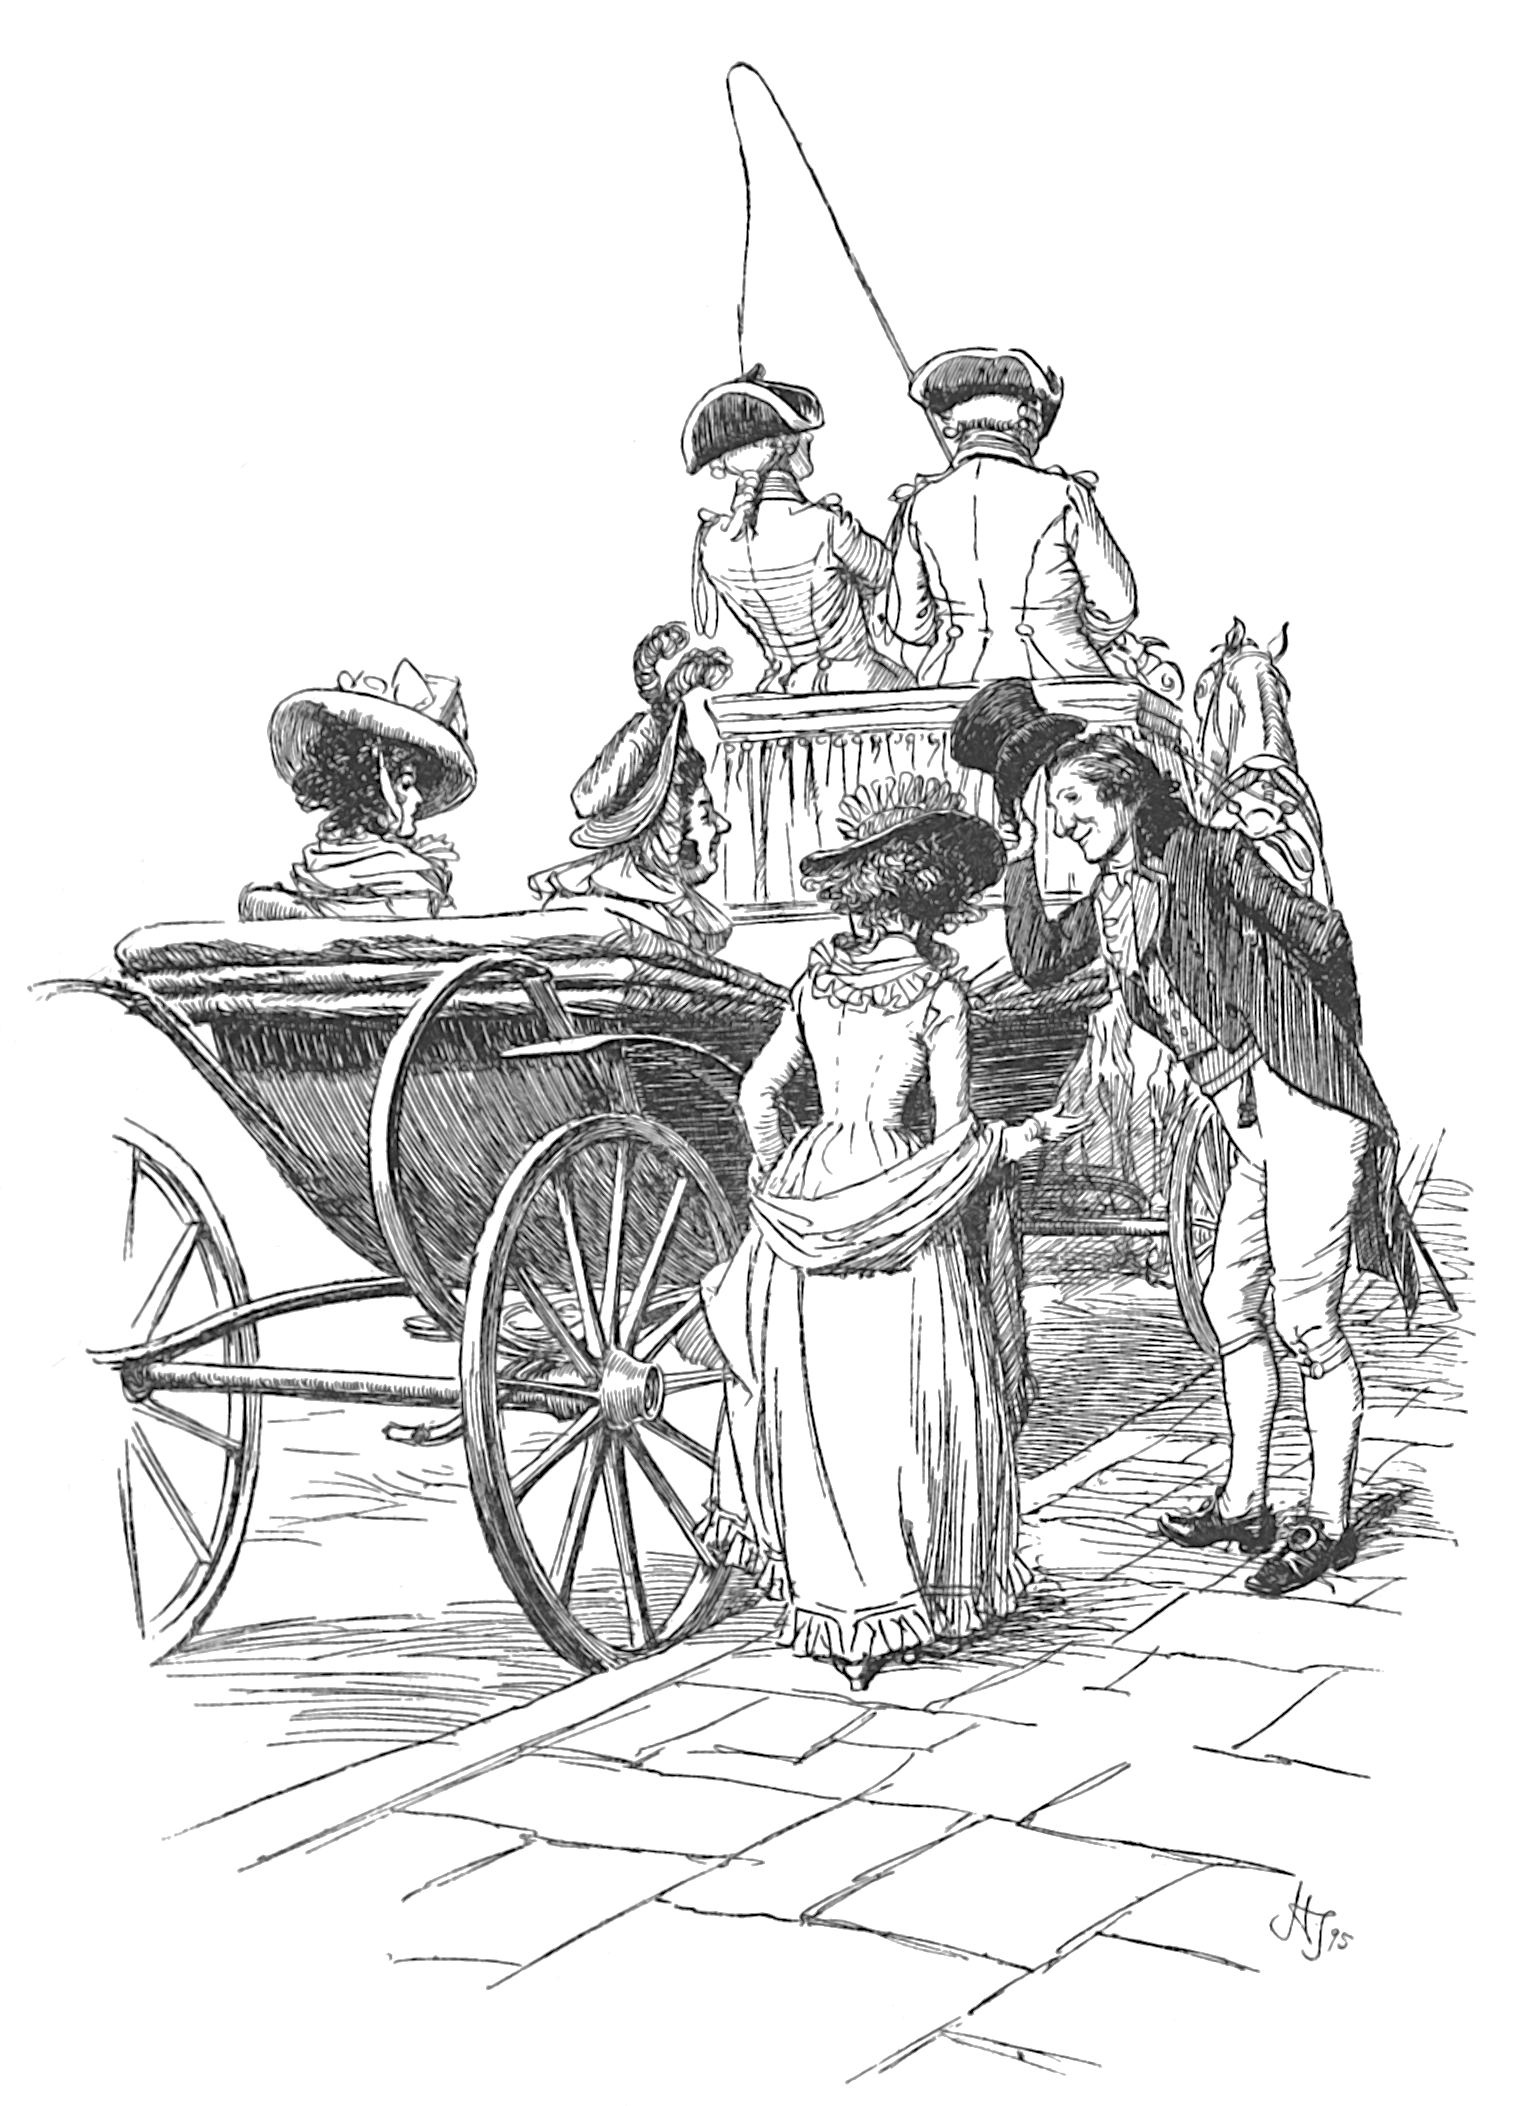
\includegraphics[width=\linewidth]{36introduced}
\caption{Mr Dashwood introduced him}
\end{figure}

He addressed her with easy civility, and twisted his head into a bow which assured her as plainly as words could have done, that he was exactly the coxcomb she had heard him described to be by Lucy. Happy had it been for her, if her regard for Edward had depended less on his own merit, than on the merit of his nearest relations! For then his brother’s bow must have given the finishing stroke to what the ill-humour of his mother and sister would have begun. But while she wondered at the difference of the two young men, she did not find that the emptiness and conceit of the one, put her out of all charity with the modesty and worth of the other. Why they \textit{were} different, Robert explained to her himself in the course of a quarter of an hour’s conversation; for, talking of his brother, and lamenting the extreme \textit{gaucherie} which he really believed kept him from mixing in proper society, he candidly and generously attributed it much less to any natural deficiency, than to the misfortune of a private education; while he himself, though probably without any particular, any material superiority by nature, merely from the advantage of a public school, was as well fitted to mix in the world as any other man.

»Upon my soul,« he added, »I believe it is nothing more; and so I often tell my mother, when she is grieving about it. »My dear Madam,« I always say to her, »you must make yourself easy. The evil is now irremediable, and it has been entirely your own doing. Why would you be persuaded by my uncle, Sir Robert, against your own judgment, to place Edward under private tuition, at the most critical time of his life? If you had only sent him to Westminster as well as myself, instead of sending him to Mr Pratt’s, all this would have been prevented.« This is the way in which I always consider the matter, and my mother is perfectly convinced of her error.«

Elinor would not oppose his opinion, because, whatever might be her general estimation of the advantage of a public school, she could not think of Edward’s abode in Mr Pratt’s family, with any satisfaction.

»You reside in Devonshire, I think,«—was his next observation, »in a cottage near Dawlish.«

Elinor set him right as to its situation; and it seemed rather surprising to him that anybody could live in Devonshire, without living near Dawlish. He bestowed his hearty approbation however on their species of house.

»For my own part,« said he, »I am excessively fond of a cottage; there is always so much comfort, so much elegance about them. And I protest, if I had any money to spare, I should buy a little land and build one myself, within a short distance of London, where I might drive myself down at any time, and collect a few friends about me, and be happy. I advise every body who is going to build, to build a cottage. My friend Lord Courtland came to me the other day on purpose to ask my advice, and laid before me three different plans of Bonomi’s. I was to decide on the best of them. »My dear Courtland,« said I, immediately throwing them all into the fire, »do not adopt either of them, but by all means build a cottage.« And that I fancy, will be the end of it.«

»Some people imagine that there can be no accommodations, no space in a cottage; but this is all a mistake. I was last month at my friend Elliott’s, near Dartford. Lady Elliott wished to give a dance. »But how can it be done?« said she; »my dear Ferrars, do tell me how it is to be managed. There is not a room in this cottage that will hold ten couple, and where can the supper be?« \textit{I} immediately saw that there could be no difficulty in it, so I said, »My dear Lady Elliott, do not be uneasy. The dining parlour will admit eighteen couple with ease; card-tables may be placed in the drawing-room; the library may be open for tea and other refreshments; and let the supper be set out in the saloon.« Lady Elliott was delighted with the thought. We measured the dining-room, and found it would hold exactly eighteen couple, and the affair was arranged precisely after my plan. So that, in fact, you see, if people do but know how to set about it, every comfort may be as well enjoyed in a cottage as in the most spacious dwelling.«

Elinor agreed to it all, for she did not think he deserved the compliment of rational opposition.

As John Dashwood had no more pleasure in music than his eldest sister, his mind was equally at liberty to fix on any thing else; and a thought struck him during the evening, which he communicated to his wife, for her approbation, when they got home. The consideration of Mrs Dennison’s mistake, in supposing his sisters their guests, had suggested the propriety of their being really invited to become such, while Mrs Jennings’s engagements kept her from home. The expense would be nothing, the inconvenience not more; and it was altogether an attention which the delicacy of his conscience pointed out to be requisite to its complete enfranchisement from his promise to his father. Fanny was startled at the proposal.

»I do not see how it can be done,« said she, »without affronting Lady Middleton, for they spend every day with her; otherwise I should be exceedingly glad to do it. You know I am always ready to pay them any attention in my power, as my taking them out this evening shows. But they are Lady Middleton’s visitors. How can I ask them away from her?«

Her husband, but with great humility, did not see the force of her objection. »They had already spent a week in this manner in Conduit Street, and Lady Middleton could not be displeased at their giving the same number of days to such near relations.«

Fanny paused a moment, and then, with fresh vigor, said,

»My love, I would ask them with all my heart, if it was in my power. But I had just settled within myself to ask the Miss Steeles to spend a few days with us. They are very well behaved, good kind of girls; and I think the attention is due to them, as their uncle did so very well by Edward. We can ask your sisters some other year, you know; but the Miss Steeles may not be in town any more. I am sure you will like them; indeed, you \textit{do} like them, you know, very much already, and so does my mother; and they are such favourites with Harry!«

Mr Dashwood was convinced. He saw the necessity of inviting the Miss Steeles immediately, and his conscience was pacified by the resolution of inviting his sisters another year; at the same time, however, slyly suspecting that another year would make the invitation needless, by bringing Elinor to town as Colonel Brandon’s wife, and Marianne as \textit{their} visitor.

Fanny, rejoicing in her escape, and proud of the ready wit that had procured it, wrote the next morning to Lucy, to request her company and her sister’s, for some days, in Harley Street, as soon as Lady Middleton could spare them. This was enough to make Lucy really and reasonably happy. Mrs Dashwood seemed actually working for her, herself; cherishing all her hopes, and promoting all her views! Such an opportunity of being with Edward and his family was, above all things, the most material to her interest, and such an invitation the most gratifying to her feelings! It was an advantage that could not be too gratefully acknowledged, nor too speedily made use of; and the visit to Lady Middleton, which had not before had any precise limits, was instantly discovered to have been always meant to end in two days’ time.

When the note was shown to Elinor, as it was within ten minutes after its arrival, it gave her, for the first time, some share in the expectations of Lucy; for such a mark of uncommon kindness, vouchsafed on so short an acquaintance, seemed to declare that the good-will towards her arose from something more than merely malice against herself; and might be brought, by time and address, to do every thing that Lucy wished. Her flattery had already subdued the pride of Lady Middleton, and made an entry into the close heart of Mrs John Dashwood; and these were effects that laid open the probability of greater.

The Miss Steeles removed to Harley Street, and all that reached Elinor of their influence there, strengthened her expectation of the event. Sir John, who called on them more than once, brought home such accounts of the favour they were in, as must be universally striking. Mrs Dashwood had never been so much pleased with any young women in her life, as she was with them; had given each of them a needle book made by some emigrant; called Lucy by her Christian name; and did not know whether she should ever be able to part with them.
%!TeX root=../pridetop.tex
\chapter[Chapter \thechapter]{}
	
\begin{figure}[t!]
\centering
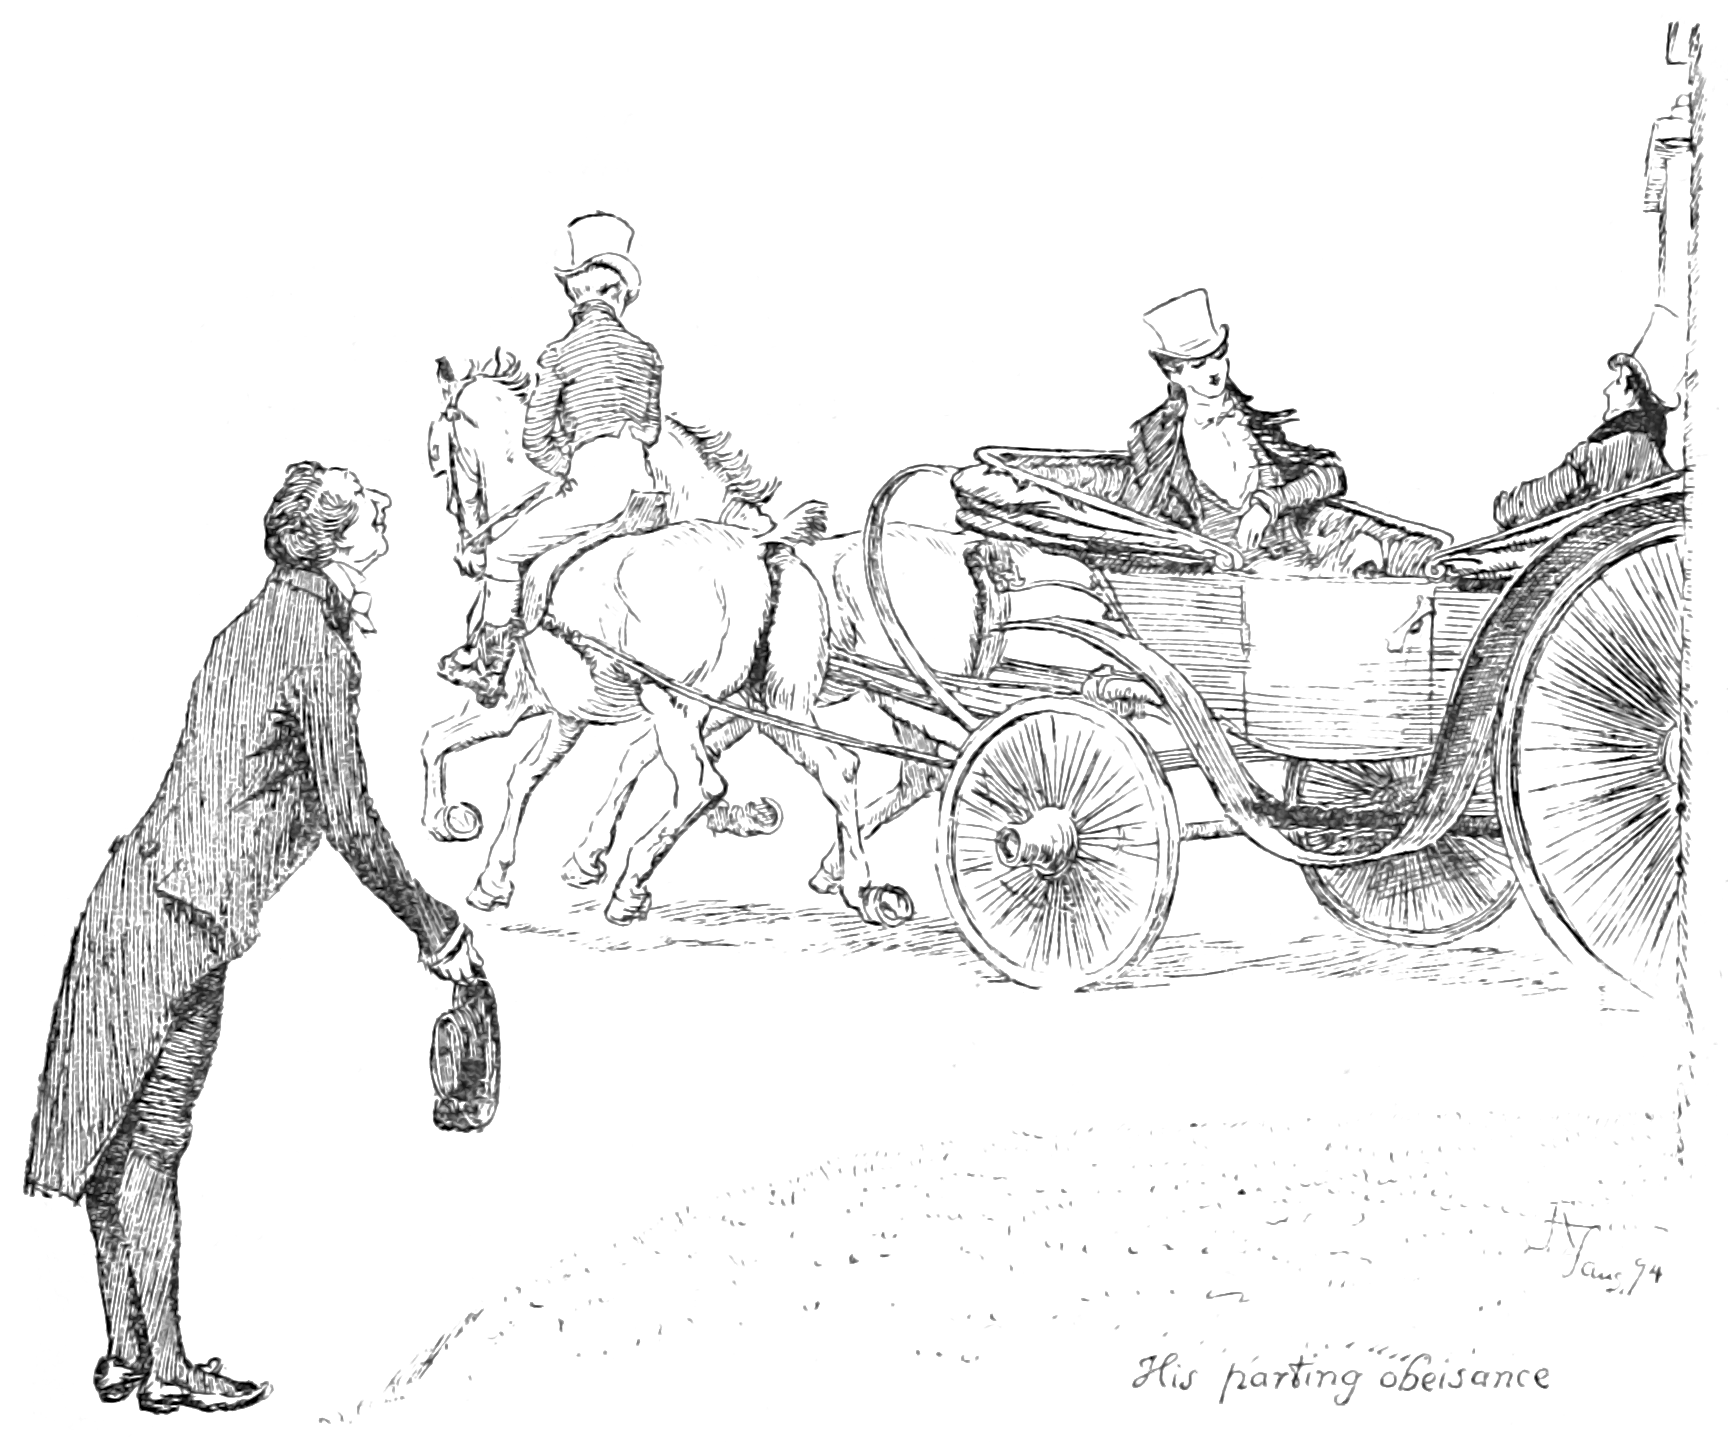
\includegraphics[width=\linewidth]{37top}
\captionlistentry{His parting obeisance}
\end{figure}


\lettrine[lines=6,image=true]{initials/chap37t}{he} two gentlemen left Rosings the next morning; and Mr Collins having been in waiting near the lodges, to make them his parting obeisance, was able to bring home the pleasing intelligence of their appearing in very good health, and in as tolerable spirits as could be expected, after the melancholy scene so lately gone through at Rosings. To Rosings he then hastened to console Lady Catherine and her daughter; and on his return brought back, with great satisfaction, a message from her Ladyship, importing that she felt herself so dull as to make her very desirous of having them all to dine with her.

Elizabeth could not see Lady Catherine without recollecting that, had she chosen it, she might by this time have been presented to her as her future niece; nor could she think, without a smile, of what her Ladyship's indignation would have been. »What would she have said? how would she have behaved?« were the questions with which she amused herself.

Their first subject was the diminution of the Rosings' party. »I assure you, I feel it exceedingly,« said Lady Catherine; »I believe nobody feels the loss of friends so much as I do. But I am particularly attached to these young men; and know them to be so much attached to me! They were excessively sorry to go! But so they always are. The dear Colonel rallied his spirits tolerably till just at last; but Darcy seemed to feel it most acutely—more, I think, than last year. His attachment to Rosings certainly increases.«

Mr Collins had a compliment and an allusion to throw in here, which were kindly smiled on by the mother and daughter.

Lady Catherine observed, after dinner, that Miss Bennet seemed out of spirits; and immediately accounting for it herself, by supposing that she did not like to go home again so soon, she added,—

»But if that is the case, you must write to your mother to beg that you may stay a little longer. Mrs Collins will be very glad of your company, I am sure.«

»I am much obliged to your Ladyship for your kind invitation,« replied Elizabeth; »but it is not in my power to accept it. I must be in town next Saturday.«

»Why, at that rate, you will have been here only six weeks. I expected you to stay two months. I told Mrs Collins so before you came. There can be no occasion for your going so soon. Mrs Bennet could certainly spare you for another fortnight.«

»But my father cannot. He wrote last week to hurry my return.«

»Oh, your father, of course, may spare you, if your mother can. Daughters are never of so much consequence to a father. And if you will stay another \textit{month} complete, it will be in my power to take one of you as far as London, for I am going there early in June, for a week; and as Dawson does not object to the barouche-box, there will be very good room for one of you—and, indeed, if the weather should happen to be cool, I should not object to taking you both, as you are neither of you large.«

\begin{figure}[tbh]
\centering
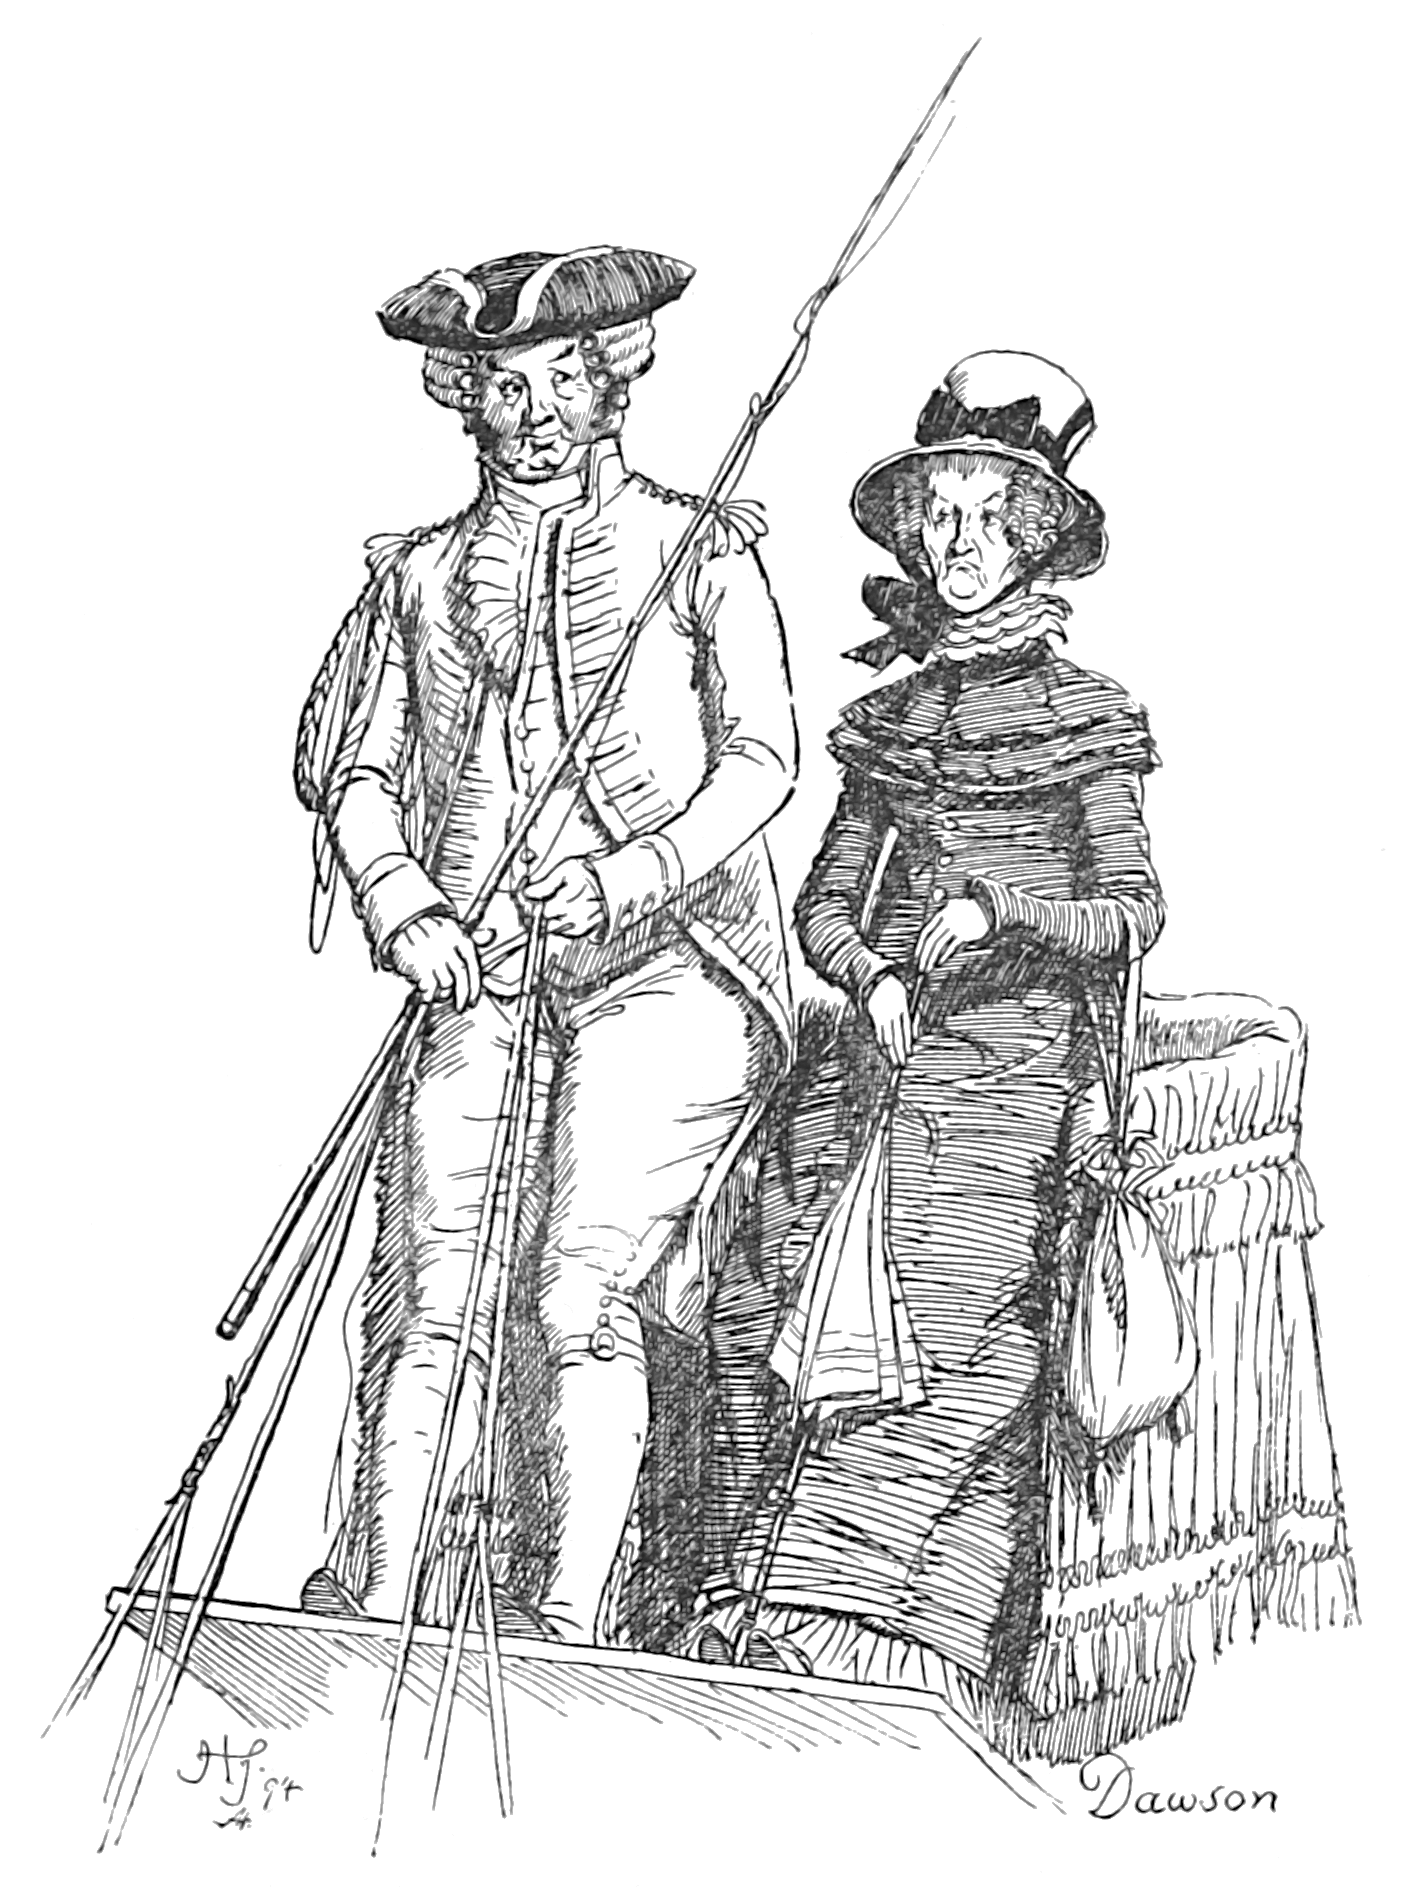
\includegraphics[width=.7\linewidth]{37dawson}
\captionlistentry{Dawson}
\end{figure}

»You are all kindness, madam; but I believe we must abide by our original plan.«

Lady Catherine seemed resigned. »Mrs Collins, you must send a servant with them. You know I always speak my mind, and I cannot bear the idea of two young women travelling post by themselves. It is highly improper. You must contrive to send somebody. I have the greatest dislike in the world to that sort of thing. Young women should always be properly guarded and attended, according to their situation in life. When my niece Georgiana went to Ramsgate last summer, I made a point of her having two men-servants go with her. Miss Darcy, the daughter of Mr Darcy of Pemberley, and Lady Anne, could not have appeared with propriety in a different manner. I am excessively attentive to all those things. You must send John with the young ladies, Mrs Collins. I am glad it occurred to me to mention it; for it would really be discreditable to \textit{you} to let them go alone.«

»My uncle is to send a servant for us.«

»Oh! Your uncle! He keeps a man-servant, does he? I am very glad you have somebody who thinks of those things. Where shall you change horses? Oh, Bromley, of course. If you mention my name at the Bell, you will be attended to.«

Lady Catherine had many other questions to ask respecting their journey; and as she did not answer them all herself attention was necessary—which Elizabeth believed to be lucky for her; or, with a mind so occupied, she might have forgotten where she was. Reflection must be reserved for solitary hours: whenever she was alone, she gave way to it as the greatest relief; and not a day went by without a solitary walk, in which she might indulge in all the delight of unpleasant recollections.

Mr Darcy's letter she was in a fair way of soon knowing by heart. She studied every sentence; and her feelings towards its writer were at times widely different. When she remembered the style of his address, she was still full of indignation: but when she considered how unjustly she had condemned and upbraided him, her anger was turned against herself; and his disappointed feelings became the object of compassion. His attachment excited gratitude, his general character respect: but she could not approve him; nor could she for a moment repent her refusal, or feel the slightest inclination ever to see him again. In her own past behaviour, there was a constant source of vexation and regret: and in the unhappy defects of her family, a subject of yet heavier chagrin. They were hopeless of remedy. Her father, contented with laughing at them, would never exert himself to restrain the wild giddiness of his youngest daughters; and her mother, with manners so far from right herself, was entirely insensible of the evil. Elizabeth had frequently united with Jane in an endeavour to check the imprudence of Catherine and Lydia; but while they were supported by their mother's indulgence, what chance could there be of improvement? Catherine, weak-spirited, irritable, and completely under Lydia's guidance, had been always affronted by their advice; and Lydia, self-willed and careless, would scarcely give them a hearing. They were ignorant, idle, and vain. While there was an officer in Meryton, they would flirt with him; and while Meryton was within a walk of Longbourn, they would be going there for ever.

Anxiety on Jane's behalf was another prevailing concern; and Mr Darcy's explanation, by restoring Bingley to all her former good opinion, heightened the sense of what Jane had lost. His affection was proved to have been sincere, and his conduct cleared of all blame, unless any could attach to the implicitness of his confidence in his friend. How grievous then was the thought that, of a situation so desirable in every respect, so replete with advantage, so promising for happiness, Jane had been deprived, by the folly and indecorum of her own family!

When to these recollections was added the development of Wickham's character, it may be easily believed that the happy spirits which had seldom been depressed before were now so much affected as to make it almost impossible for her to appear tolerably cheerful.

Their engagements at Rosings were as frequent during the last week of her stay as they had been at first. The very last evening was spent there; and her Ladyship again inquired minutely into the particulars of their journey, gave them directions as to the best method of packing, and was so urgent on the necessity of placing gowns in the only right way, that Maria thought herself obliged, on her return, to undo all the work of the morning, and pack her trunk afresh.

When they parted, Lady Catherine, with great condescension, wished them a good journey, and invited them to come to Hunsford again next year; and Miss de Bourgh exerted herself so far as to courtesy and hold out her hand to both.
%!TeX root=../sensetop.tex
\chapter[Chapter \thechapter]{}
\lettrine[lines=4,lraise=0.3]{M}{rs} Jennings was very warm in her praise of Edward’s conduct, but only Elinor and Marianne understood its true merit. \textit{They} only knew how little he had had to tempt him to be disobedient, and how small was the consolation, beyond the consciousness of doing right, that could remain to him in the loss of friends and fortune. Elinor gloried in his integrity; and Marianne forgave all his offences in compassion for his punishment. But though confidence between them was, by this public discovery, restored to its proper state, it was not a subject on which either of them were fond of dwelling when alone. Elinor avoided it upon principle, as tending to fix still more upon her thoughts, by the too warm, too positive assurances of Marianne, that belief of Edward’s continued affection for herself which she rather wished to do away; and Marianne’s courage soon failed her, in trying to converse upon a topic which always left her more dissatisfied with herself than ever, by the comparison it necessarily produced between Elinor’s conduct and her own.

She felt all the force of that comparison; but not as her sister had hoped, to urge her to exertion now; she felt it with all the pain of continual self-reproach, regretted most bitterly that she had never exerted herself before; but it brought only the torture of penitence, without the hope of amendment. Her mind was so much weakened that she still fancied present exertion impossible, and therefore it only dispirited her more.

Nothing new was heard by them, for a day or two afterwards, of affairs in Harley Street, or Bartlett’s Buildings. But though so much of the matter was known to them already, that Mrs Jennings might have had enough to do in spreading that knowledge farther, without seeking after more, she had resolved from the first to pay a visit of comfort and inquiry to her cousins as soon as she could; and nothing but the hindrance of more visitors than usual, had prevented her going to them within that time.

The third day succeeding their knowledge of the particulars, was so fine, so beautiful a Sunday as to draw many to Kensington Gardens, though it was only the second week in March. Mrs Jennings and Elinor were of the number; but Marianne, who knew that the Willoughbys were again in town, and had a constant dread of meeting them, chose rather to stay at home, than venture into so public a place.

An intimate acquaintance of Mrs Jennings joined them soon after they entered the Gardens, and Elinor was not sorry that by her continuing with them, and engaging all Mrs Jennings’s conversation, she was herself left to quiet reflection. She saw nothing of the Willoughbys, nothing of Edward, and for some time nothing of anybody who could by any chance whether grave or gay, be interesting to her. But at last she found herself with some surprise, accosted by Miss Steele, who, though looking rather shy, expressed great satisfaction in meeting them, and on receiving encouragement from the particular kindness of Mrs Jennings, left her own party for a short time, to join their’s. Mrs Jennings immediately whispered to Elinor,

»Get it all out of her, my dear. She will tell you any thing if you ask. You see I cannot leave Mrs Clarke.«

It was lucky, however, for Mrs Jennings’s curiosity and Elinor’s too, that she would tell any thing \textit{without} being asked; for nothing would otherwise have been learnt.

»I am so glad to meet you;« said Miss Steele, taking her familiarly by the arm—»for I wanted to see you of all things in the world.« And then lowering her voice, »I suppose Mrs Jennings has heard all about it. Is she angry?«

»Not at all, I believe, with you.«

»That is a good thing. And Lady Middleton, is \textit{she} angry?«

»I cannot suppose it possible that she should be.«

»I am monstrous glad of it. Good gracious! I have had such a time of it! I never saw Lucy in such a rage in my life. She vowed at first she would never trim me up a new bonnet, nor do any thing else for me again, so long as she lived; but now she is quite come to, and we are as good friends as ever. Look, she made me this bow to my hat, and put in the feather last night. There now, \textit{you} are going to laugh at me too. But why should not I wear pink ribbons? I do not care if it \textit{is} the Doctor’s favourite colour. I am sure, for my part, I should never have known he \textit{did} like it better than any other colour, if he had not happened to say so. My cousins have been so plaguing me! I declare sometimes I do not know which way to look before them.«


\begin{a4}
	\begin{figure}[tbph]
		\centering
		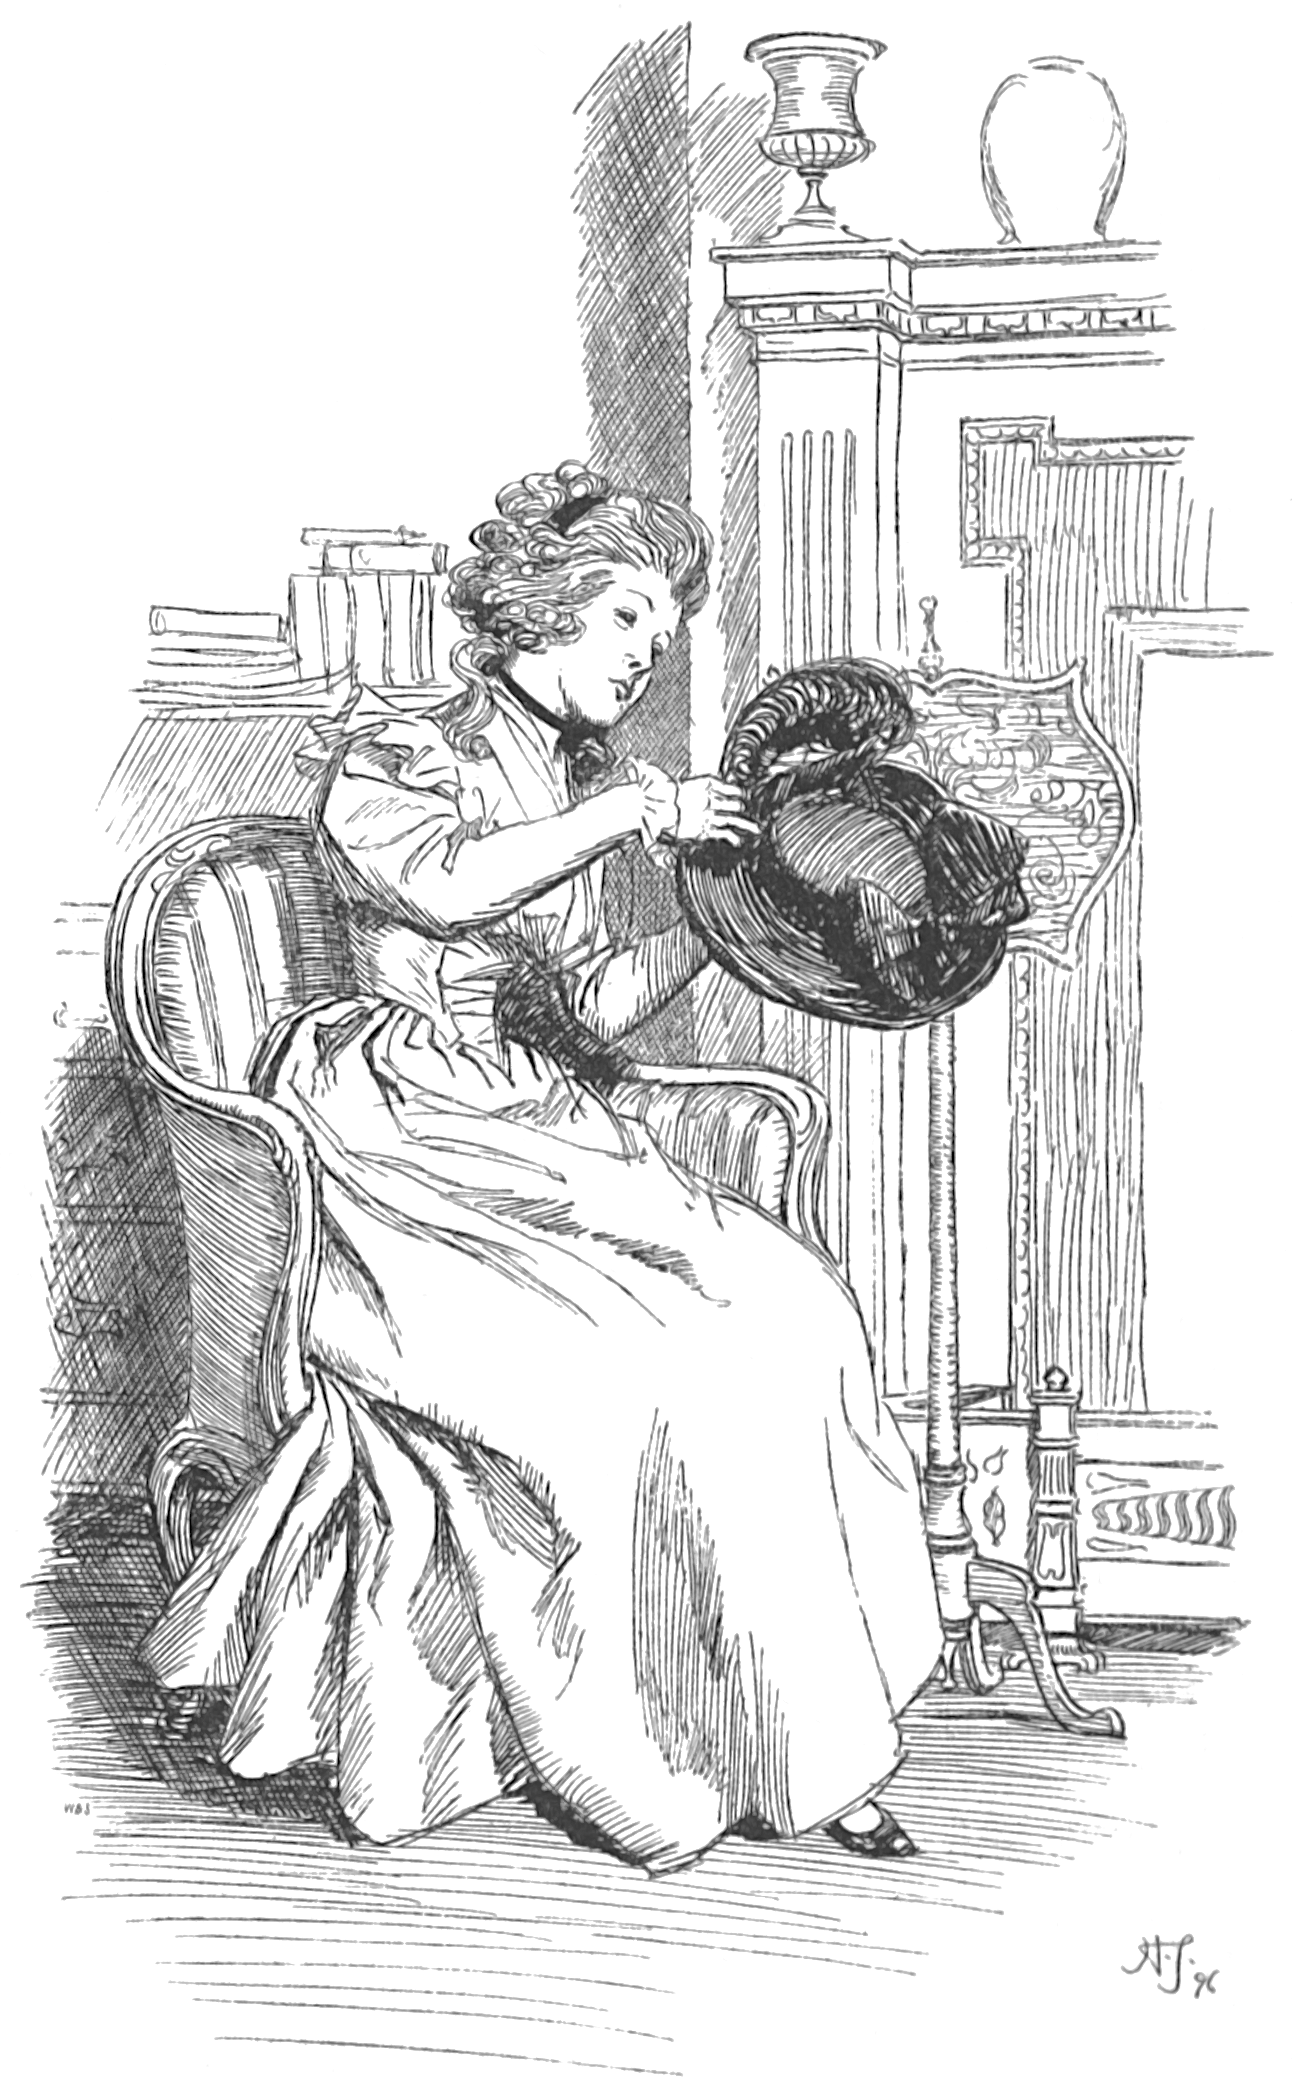
\includegraphics[width=.9\linewidth]{38feather}
		\caption{She put in the feather last night}
	\end{figure}
\end{a4}

\begin{letter}
	\begin{figure}[tbph]
		\centering
		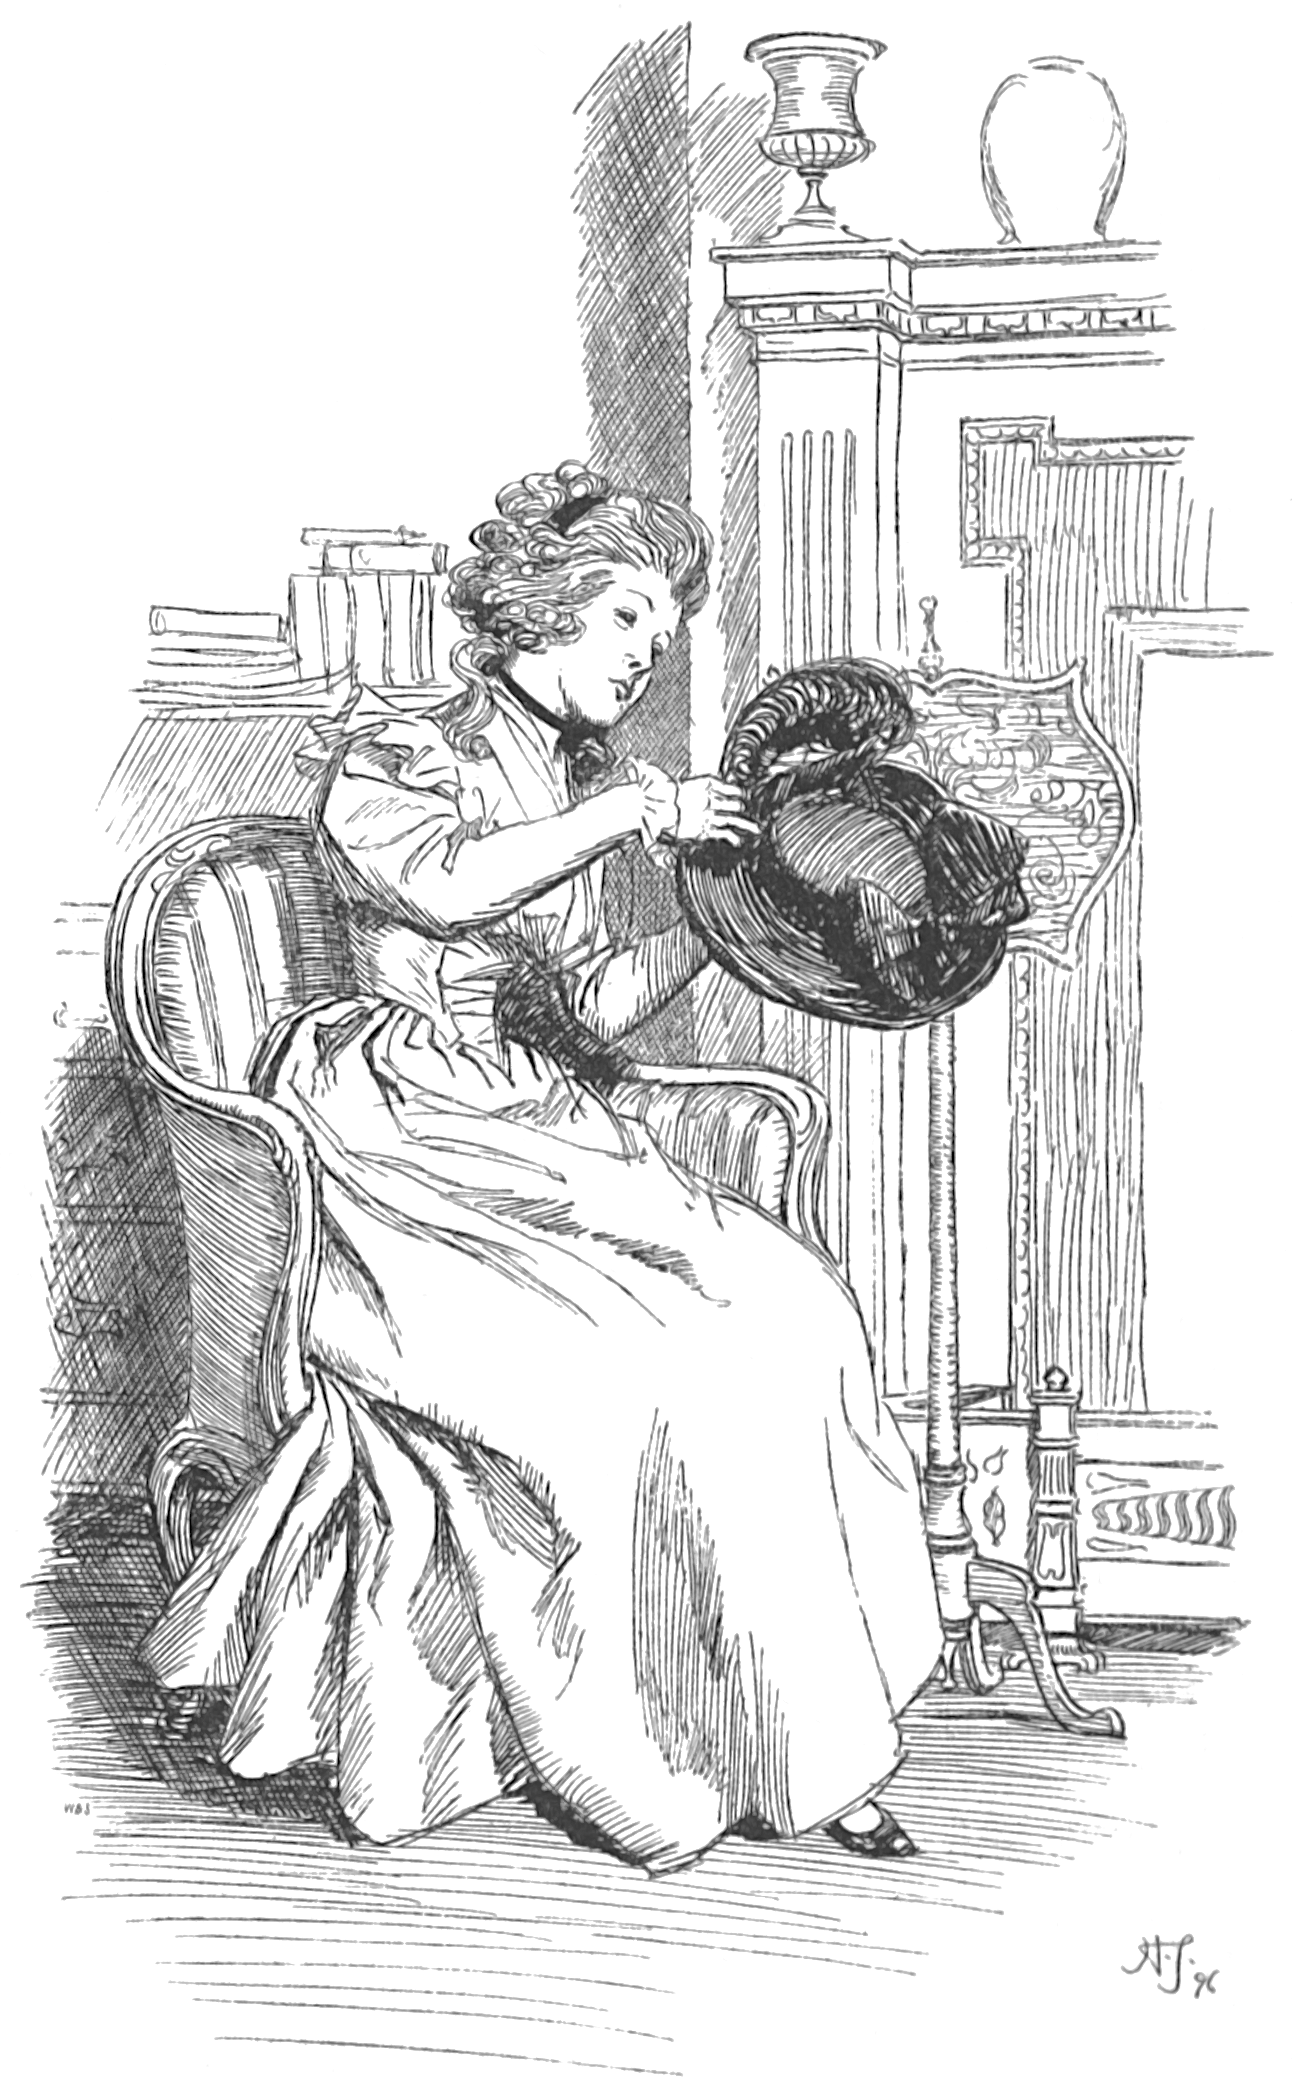
\includegraphics[width=\linewidth]{38feather}
		\caption{She put in the feather last night}
	\end{figure}
\end{letter}


She had wandered away to a subject on which Elinor had nothing to say, and therefore soon judged it expedient to find her way back again to the first.

»Well, but Miss Dashwood,« speaking triumphantly, »people may say what they chuse about Mr Ferrars’s declaring he would not have Lucy, for it is no such thing I can tell you; and it is quite a shame for such ill-natured reports to be spread abroad. Whatever Lucy might think about it herself, you know, it was no business of other people to set it down for certain.«

»I never heard any thing of the kind hinted at before, I assure you,« said Elinor.

»Oh, did not you? But it \textit{was} said, I know, very well, and by more than one; for Miss Godby told Miss Sparks, that nobody in their senses could expect Mr Ferrars to give up a woman like Miss Morton, with thirty thousand pounds to her fortune, for Lucy Steele that had nothing at all; and I had it from Miss Sparks myself. And besides that, my cousin Richard said himself, that when it came to the point he was afraid Mr Ferrars would be off; and when Edward did not come near us for three days, I could not tell what to think myself; and I believe in my heart Lucy gave it up all for lost; for we came away from your brother’s Wednesday, and we saw nothing of him not all Thursday, Friday, and Saturday, and did not know what was become of him. Once Lucy thought to write to him, but then her spirits rose against that. However this morning he came just as we came home from church; and then it all came out, how he had been sent for Wednesday to Harley Street, and been talked to by his mother and all of them, and how he had declared before them all that he loved nobody but Lucy, and nobody but Lucy would he have. And how he had been so worried by what passed, that as soon as he had went away from his mother’s house, he had got upon his horse, and rid into the country, some where or other; and how he had stayed about at an inn all Thursday and Friday, on purpose to get the better of it. And after thinking it all over and over again, he said, it seemed to him as if, now he had no fortune, and no nothing at all, it would be quite unkind to keep her on to the engagement, because it must be for her loss, for he had nothing but two thousand pounds, and no hope of any thing else; and if he was to go into orders, as he had some thoughts, he could get nothing but a curacy, and how was they to live upon that?—He could not bear to think of her doing no better, and so he begged, if she had the least mind for it, to put an end to the matter directly, and leave him shift for himself. I heard him say all this as plain as could possibly be. And it was entirely for \textit{her} sake, and upon \textit{her} account, that he said a word about being off, and not upon his own. I will take my oath he never dropt a syllable of being tired of her, or of wishing to marry Miss Morton, or any thing like it. But, to be sure, Lucy would not give ear to such kind of talking; so she told him directly (with a great deal about sweet and love, you know, and all that—Oh, la! one can’t repeat such kind of things you know)—she told him directly, she had not the least mind in the world to be off, for she could live with him upon a trifle, and how little so ever he might have, she should be very glad to have it all, you know, or something of the kind. So then he was monstrous happy, and talked on some time about what they should do, and they agreed he should take orders directly, and they must wait to be married till he got a living. And just then I could not hear any more, for my cousin called from below to tell me Mrs Richardson was come in her coach, and would take one of us to Kensington Gardens; so I was forced to go into the room and interrupt them, to ask Lucy if she would like to go, but she did not care to leave Edward; so I just run up stairs and put on a pair of silk stockings and came off with the Richardsons.«

»I do not understand what you mean by interrupting them,« said Elinor; »you were all in the same room together, were not you?«

»No, indeed, not us. La! Miss Dashwood, do you think people make love when any body else is by? Oh, for shame!—To be sure you must know better than that. (Laughing affectedly.)—No, no; they were shut up in the drawing-room together, and all I heard was only by listening at the door.«

»How!« cried Elinor; »have you been repeating to me what you only learnt yourself by listening at the door? I am sorry I did not know it before; for I certainly would not have suffered you to give me particulars of a conversation which you ought not to have known yourself. How could you behave so unfairly by your sister?«

\begin{a4}
	\begin{figure}[tbph]
		\centering
		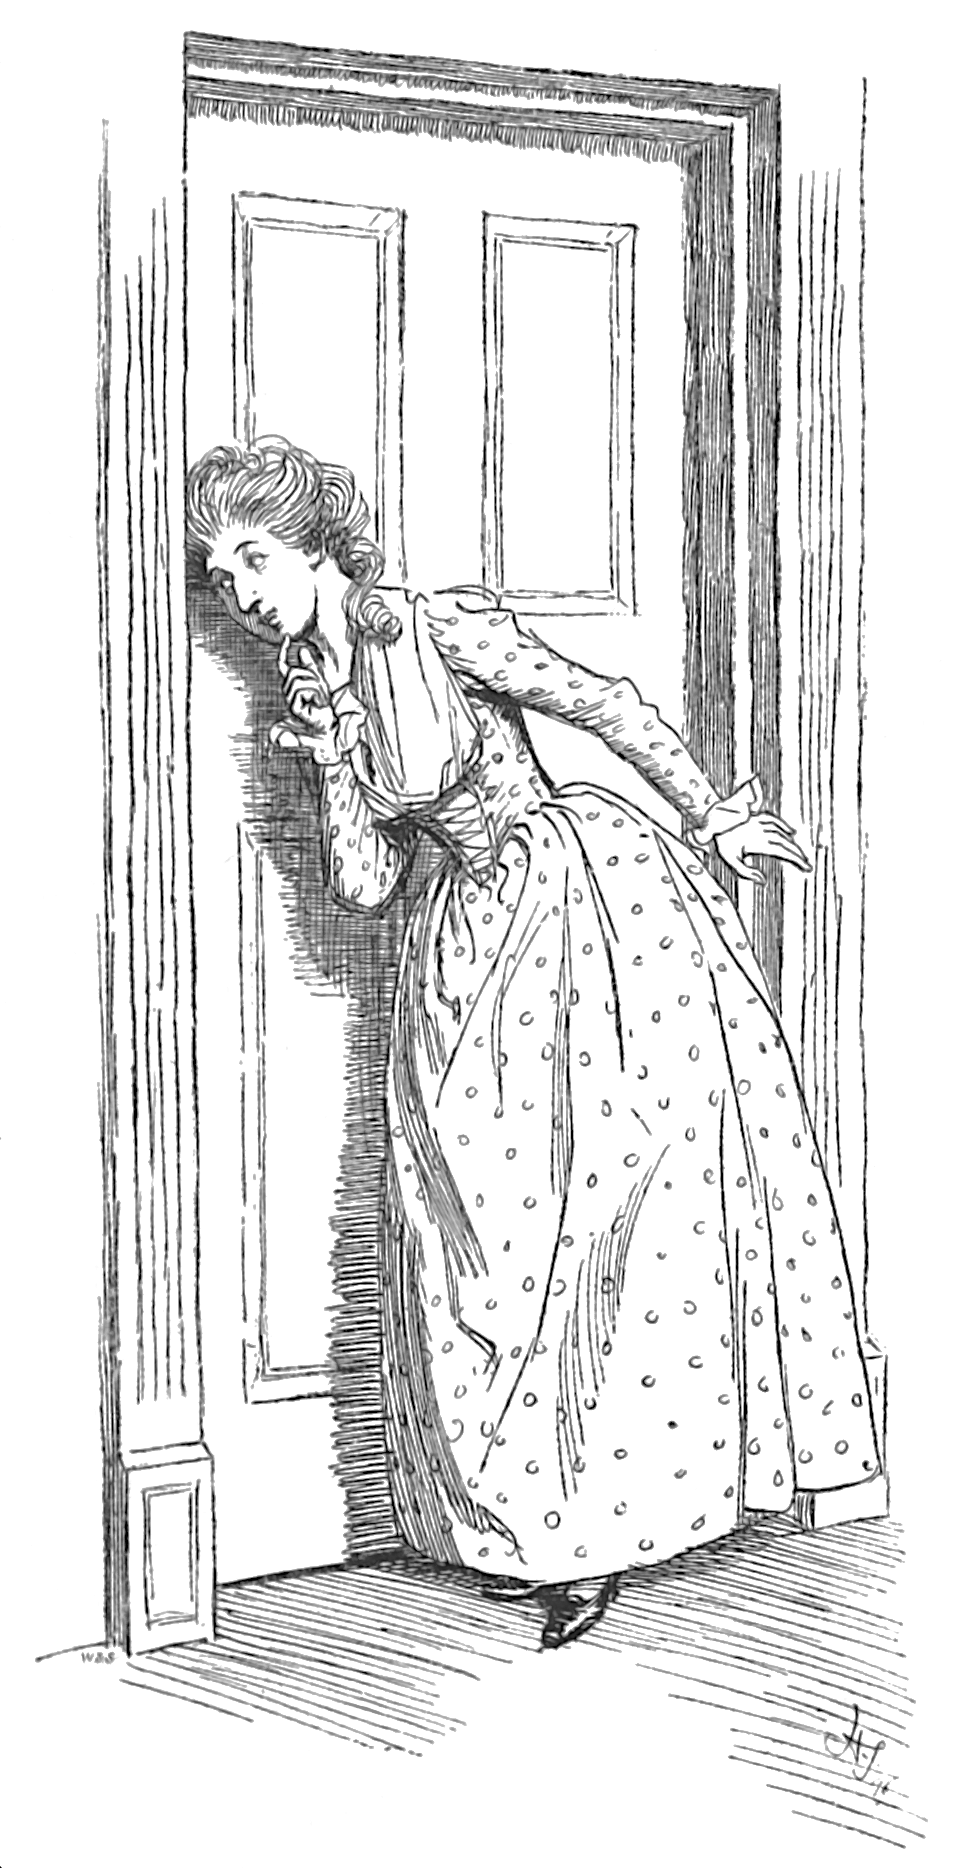
\includegraphics[width=.7\linewidth]{38listen}
		\caption{Listening at the door}
	\end{figure}
\end{a4}


\begin{letter}
	\begin{figure}[tbph]
		\centering
		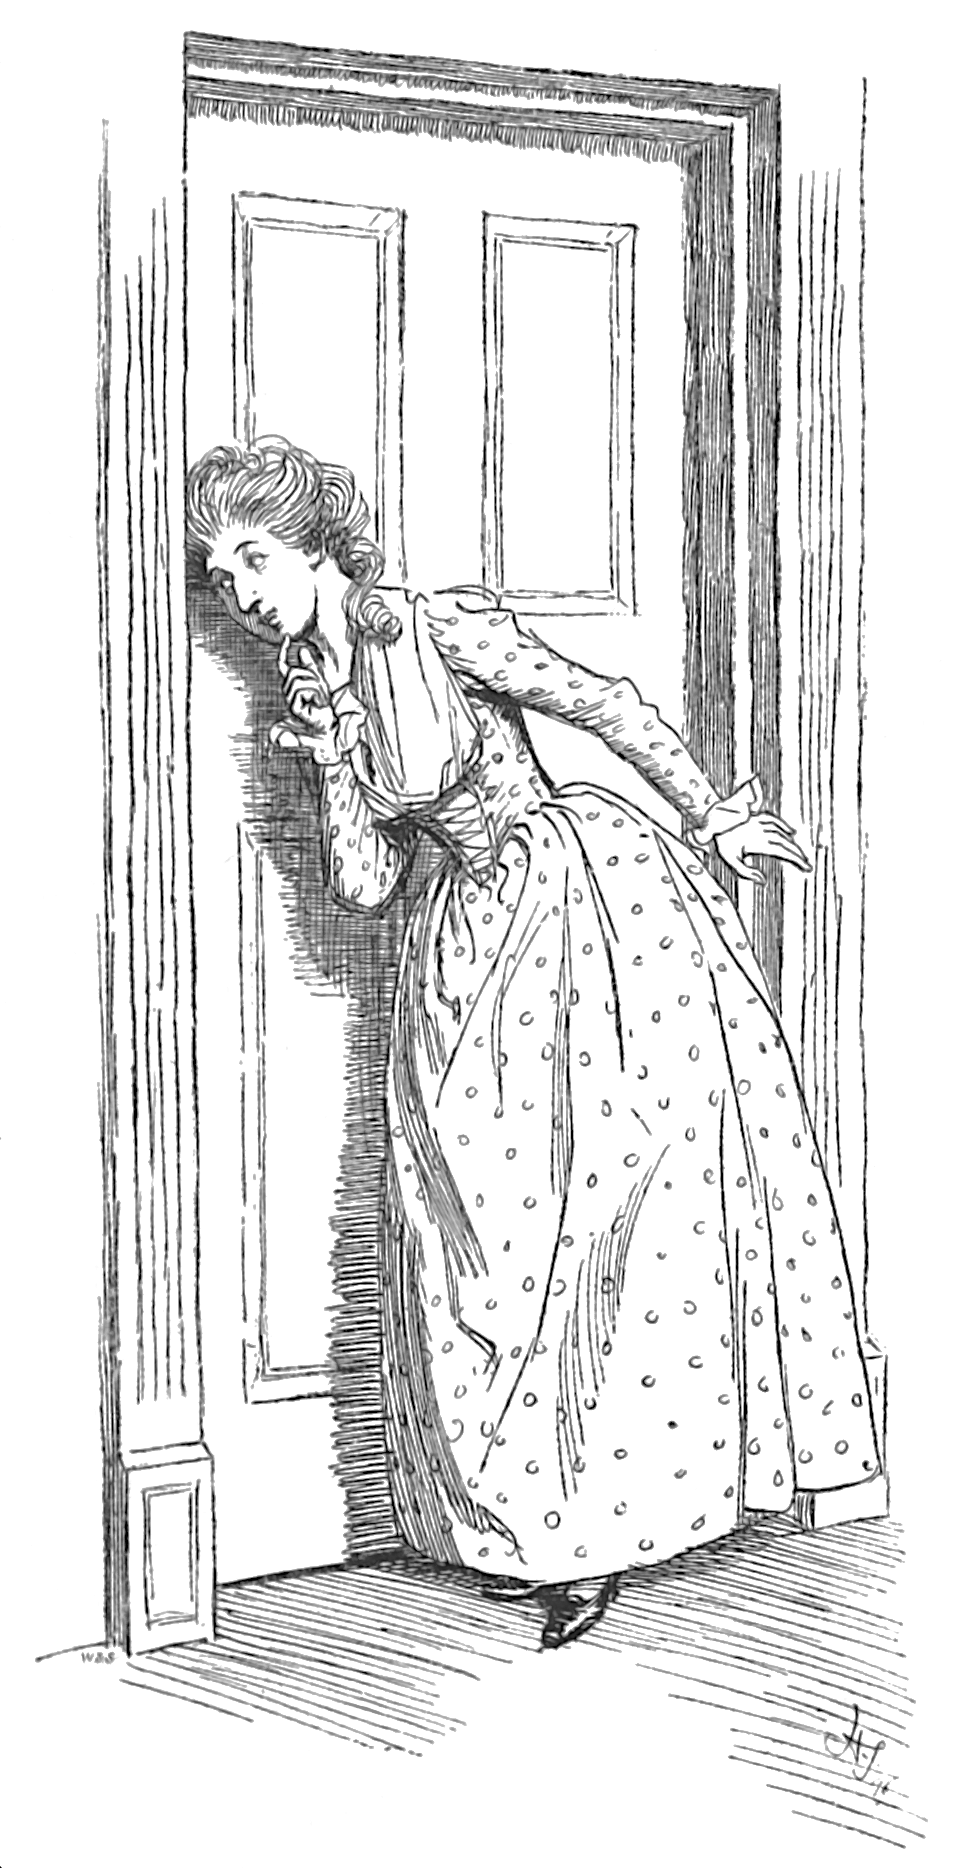
\includegraphics[width=.8\linewidth]{38listen}
		\caption{Listening at the door}
	\end{figure}
\end{letter}



»Oh, la! there is nothing in \textit{that}. I only stood at the door, and heard what I could. And I am sure Lucy would have done just the same by me; for a year or two back, when Martha Sharpe and I had so many secrets together, she never made any bones of hiding in a closet, or behind a chimney-board, on purpose to hear what we said.«

Elinor tried to talk of something else; but Miss Steele could not be kept beyond a couple of minutes, from what was uppermost in her mind.

»Edward talks of going to Oxford soon,« said she; »but now he is lodging at No.—, Pall Mall. What an ill-natured woman his mother is, an’t she? And your brother and sister were not very kind! However, I shan’t say anything against them to \textit{you}; and to be sure they did send us home in their own chariot, which was more than I looked for. And for my part, I was all in a fright for fear your sister should ask us for the huswifes she had gave us a day or two before; but, however, nothing was said about them, and I took care to keep mine out of sight. Edward have got some business at Oxford, he says; so he must go there for a time; and after \textit{that}, as soon as he can light upon a Bishop, he will be ordained. I wonder what curacy he will get! Good gracious! (giggling as she spoke) I’d lay my life I know what my cousins will say, when they hear of it. They will tell me I should write to the Doctor, to get Edward the curacy of his new living. I know they will; but I am sure I would not do such a thing for all the world. »La!« I shall say directly, »I wonder how you could think of such a thing? \textit{I} write to the Doctor, indeed!««

»Well,« said Elinor, »it is a comfort to be prepared against the worst. You have got your answer ready.«

Miss Steele was going to reply on the same subject, but the approach of her own party made another more necessary.

»Oh, la! here come the Richardsons. I had a vast deal more to say to you, but I must not stay away from them not any longer. I assure you they are very genteel people. He makes a monstrous deal of money, and they keep their own coach. I have not time to speak to Mrs Jennings about it myself, but pray tell her I am quite happy to hear she is not in anger against us, and Lady Middleton the same; and if anything should happen to take you and your sister away, and Mrs Jennings should want company, I am sure we should be very glad to come and stay with her for as long a time as she likes. I suppose Lady Middleton won’t ask us any more this bout. Good-by; I am sorry Miss Marianne was not here. Remember me kindly to her. La! if you have not got your spotted muslin on!—I wonder you was not afraid of its being torn.«

Such was her parting concern; for after this, she had time only to pay her farewell compliments to Mrs Jennings, before her company was claimed by Mrs Richardson; and Elinor was left in possession of knowledge which might feed her powers of reflection some time, though she had learnt very little more than what had been already foreseen and foreplanned in her own mind. Edward’s marriage with Lucy was as firmly determined on, and the time of its taking place remained as absolutely uncertain, as she had concluded it would be;—every thing depended, exactly after her expectation, on his getting that preferment, of which, at present, there seemed not the smallest chance.

As soon as they returned to the carriage, Mrs Jennings was eager for information; but as Elinor wished to spread as little as possible intelligence that had in the first place been so unfairly obtained, she confined herself to the brief repetition of such simple particulars, as she felt assured that Lucy, for the sake of her own consequence, would choose to have known. The continuance of their engagement, and the means that were able to be taken for promoting its end, was all her communication; and this produced from Mrs Jennings the following natural remark.

»Wait for his having a living!—ay, we all know how \textit{that} will end:—they will wait a twelvemonth, and finding no good comes of it, will set down upon a curacy of fifty pounds a-year, with the interest of his two thousand pounds, and what little matter Mr Steele and Mr Pratt can give her. Then they will have a child every year! and Lord help ’em! how poor they will be! I must see what I can give them towards furnishing their house. Two maids and two men, indeed! as I talked of t’ other day. No, no, they must get a stout girl of all works. Betty’s sister would never do for them \textit{now}.«

The next morning brought Elinor a letter by the two-penny post from Lucy herself. It was as follows:

\begin{quotation}
\begin{flushright}
Bartlett’s Building, March.
\end{flushright}
~\\
\indent I hope my dear Miss Dashwood will excuse the liberty I take of writing to her; but I know your friendship for me will make you pleased to hear such a good account of myself and my dear Edward, after all the troubles we have went through lately, therefore will make no more apologies, but proceed to say that, thank God! though we have suffered dreadfully, we are both quite well now, and as happy as we must always be in one another’s love. We have had great trials, and great persecutions, but however, at the same time, gratefully acknowledge many friends, yourself not the least among them, whose great kindness I shall always thankfully remember, as will Edward too, who I have told of it. I am sure you will be glad to hear, as likewise dear Mrs Jennings, I spent two happy hours with him yesterday afternoon, he would not hear of our parting, though earnestly did I, as I thought my duty required, urge him to it for prudence sake, and would have parted for ever on the spot, would he consent to it; but he said it should never be, he did not regard his mother’s anger, while he could have my affections; our prospects are not very bright, to be sure, but we must wait, and hope for the best; he will be ordained shortly; and should it ever be in your power to recommend him to any body that has a living to bestow, am very sure you will not forget us, and dear Mrs Jennings too, trust she will speak a good word for us to Sir John, or Mr Palmer, or any friend that may be able to assist us.—Poor Anne was much to blame for what she did, but she did it for the best, so I say nothing; hope Mrs Jennings won’t think it too much trouble to give us a call, should she come this way any morning, ’twould be a great kindness, and my cousins would be proud to know her.—My paper reminds me to conclude; and begging to be most gratefully and respectfully remembered to her, and to Sir John, and Lady Middleton, and the dear children, when you chance to see them, and love to Miss Marianne,
\begin{flushright}
I am, \&c.
\end{flushright}
\end{quotation}

As soon as Elinor had finished it, she performed what she concluded to be its writer’s real design, by placing it in the hands of Mrs Jennings, who read it aloud with many comments of satisfaction and praise.

»Very well indeed!—how prettily she writes!—aye, that was quite proper to let him be off if he would. That was just like Lucy. Poor soul! I wish I \textit{could} get him a living, with all my heart. She calls me dear Mrs Jennings, you see. She is a good-hearted girl as ever lived. Very well upon my word. That sentence is very prettily turned. Yes, yes, I will go and see her, sure enough. How attentive she is, to think of every body!—Thank you, my dear, for showing it me. It is as pretty a letter as ever I saw, and does Lucy’s head and heart great credit.«
%!TeX root=../sensetop.tex
\chapter[Chapter \thechapter]{}
\lettrine[lraise=0.3]{T}{he} Miss Dashwoods had now been rather more than two months in town, and Marianne's impatience to be gone increased every day. She sighed for the air, the liberty, the quiet of the country; and fancied that if any place could give her ease, Barton must do it. Elinor was hardly less anxious than herself for their removal, and only so much less bent on its being effected immediately, as that she was conscious of the difficulties of so long a journey, which Marianne could not be brought to acknowledge. She began, however, seriously to turn her thoughts towards its accomplishment, and had already mentioned their wishes to their kind hostess, who resisted them with all the eloquence of her good-will, when a plan was suggested, which, though detaining them from home yet a few weeks longer, appeared to Elinor altogether much more eligible than any other. The Palmers were to remove to Cleveland about the end of March, for the Easter holidays; and Mrs Jennings, with both her friends, received a very warm invitation from Charlotte to go with them. This would not, in itself, have been sufficient for the delicacy of Miss Dashwood;—but it was inforced with so much real politeness by Mr Palmer himself, as, joined to the very great amendment of his manners towards them since her sister had been known to be unhappy, induced her to accept it with pleasure.

When she told Marianne what she had done, however, her first reply was not very auspicious.

<Cleveland!>—she cried, with great agitation. <No, I cannot go to Cleveland.>

<You forget,> said Elinor gently, <that its situation is not—that it is not in the neighbourhood of\longdash>

<But it is in Somersetshire.—I cannot go into Somersetshire.—There, where I looked forward to going...No, Elinor, you cannot expect me to go there.>

Elinor would not argue upon the propriety of overcoming such feelings;—she only endeavoured to counteract them by working on others;—represented it, therefore, as a measure which would fix the time of her returning to that dear mother, whom she so much wished to see, in a more eligible, more comfortable manner, than any other plan could do, and perhaps without any greater delay. From Cleveland, which was within a few miles of Bristol, the distance to Barton was not beyond one day, though a long day's journey; and their mother's servant might easily come there to attend them down; and as there could be no occasion of their staying above a week at Cleveland, they might now be at home in little more than three weeks' time. As Marianne's affection for her mother was sincere, it must triumph with little difficulty, over the imaginary evils she had started.

Mrs Jennings was so far from being weary of her guests, that she pressed them very earnestly to return with her again from Cleveland. Elinor was grateful for the attention, but it could not alter her design; and their mother's concurrence being readily gained, every thing relative to their return was arranged as far as it could be;—and Marianne found some relief in drawing up a statement of the hours that were yet to divide her from Barton.

<Ah! Colonel, I do not know what you and I shall do without the Miss Dashwoods;>—was Mrs Jennings's address to him when he first called on her, after their leaving her was settled—<for they are quite resolved upon going home from the Palmers;—and how forlorn we shall be, when I come back!—Lord! we shall sit and gape at one another as dull as two cats.>

Perhaps Mrs Jennings was in hopes, by this vigorous sketch of their future ennui, to provoke him to make that offer, which might give himself an escape from it; and if so, she had soon afterwards good reason to think her object gained; for, on Elinor's moving to the window to take more expeditiously the dimensions of a print, which she was going to copy for her friend, he followed her to it with a look of particular meaning, and conversed with her there for several minutes. The effect of his discourse on the lady too, could not escape her observation, for though she was too honourable to listen, and had even changed her seat, on purpose that she might \textit{not} hear, to one close by the piano forte on which Marianne was playing, she could not keep herself from seeing that Elinor changed colour, attended with agitation, and was too intent on what he said to pursue her employment. Still farther in confirmation of her hopes, in the interval of Marianne's turning from one lesson to another, some words of the Colonel's inevitably reached her ear, in which he seemed to be apologising for the badness of his house. This set the matter beyond a doubt. She wondered, indeed, at his thinking it necessary to do so; but supposed it to be the proper etiquette. What Elinor said in reply she could not distinguish, but judged from the motion of her lips, that she did not think \textit{that} any material objection; and Mrs Jennings commended her in her heart for being so honest. They then talked on for a few minutes longer without her catching a syllable, when another lucky stop in Marianne's performance brought her these words in the Colonel's calm voice,—

<I am afraid it cannot take place very soon.>

Astonished and shocked at so unlover-like a speech, she was almost ready to cry out, <Lord! what should hinder it?>—but checking her desire, confined herself to this silent ejaculation.

<This is very strange!—sure he need not wait to be older.>

This delay on the Colonel's side, however, did not seem to offend or mortify his fair companion in the least, for on their breaking up the conference soon afterwards, and moving different ways, Mrs Jennings very plainly heard Elinor say, and with a voice which showed her to feel what she said,

<I shall always think myself very much obliged to you.>

Mrs Jennings was delighted with her gratitude, and only wondered that after hearing such a sentence, the Colonel should be able to take leave of them, as he immediately did, with the utmost \textit{sang-froid}, and go away without making her any reply! She had not thought her old friend could have made so indifferent a suitor.

What had really passed between them was to this effect.

<I have heard,> said he, with great compassion, <of the injustice your friend Mr Ferrars has suffered from his family; for if I understand the matter right, he has been entirely cast off by them for persevering in his engagement with a very deserving young woman. Have I been rightly informed? Is it so?;>

Elinor told him that it was.

<The cruelty, the impolitic cruelty,> he replied, with great feeling, <of dividing, or attempting to divide, two young people long attached to each other, is terrible. Mrs Ferrars does not know what she may be doing—what she may drive her son to. I have seen Mr Ferrars two or three times in Harley Street, and am much pleased with him. He is not a young man with whom one can be intimately acquainted in a short time, but I have seen enough of him to wish him well for his own sake, and as a friend of yours, I wish it still more. I understand that he intends to take orders. Will you be so good as to tell him that the living of Delaford, now just vacant, as I am informed by this day's post, is his, if he think it worth his acceptance; but \textit{that}, perhaps, so unfortunately circumstanced as he is now, it may be nonsense to appear to doubt; I only wish it were more valuable. It is a rectory, but a small one; the late incumbent, I believe, did not make more than \textsterling 200 per annum, and though it is certainly capable of improvement, I fear, not to such an amount as to afford him a very comfortable income. Such as it is, however, my pleasure in presenting it to him, will be very great. Pray assure him of it.>

Elinor's astonishment at this commission could hardly have been greater, had the Colonel been really making her an offer of his hand. The preferment, which only two days before she had considered as hopeless for Edward, was already provided to enable him to marry; and \textit{she}, of all people in the world, was fixed on to bestow it! Her emotion was such as Mrs Jennings had attributed to a very different cause; but whatever minor feelings less pure, less pleasing, might have a share in that emotion, her esteem for the general benevolence, and her gratitude for the particular friendship, which together prompted Colonel Brandon to this act, were strongly felt, and warmly expressed. She thanked him for it with all her heart, spoke of Edward's principles and disposition with that praise which she knew them to deserve; and promised to undertake the commission with pleasure, if it were really his wish to put off so agreeable an office to another. But at the same time, she could not help thinking that no one could so well perform it as himself. It was an office in short, from which, unwilling to give Edward the pain of receiving an obligation from \textit{her}, she would have been very glad to be spared herself; but Colonel Brandon, on motives of equal delicacy, declining it likewise, still seemed so desirous of its being given through her means, that she would not on any account make farther opposition. Edward, she believed, was still in town, and fortunately she had heard his address from Miss Steele. She could undertake therefore to inform him of it, in the course of the day. After this had been settled, Colonel Brandon began to talk of his own advantage in securing so respectable and agreeable a neighbour, and \textit{then} it was that he mentioned with regret, that the house was small and indifferent; an evil which Elinor, as Mrs Jennings had supposed her to do, made very light of, at least as far as regarded its size.

<The smallness of the house,> said she, <I cannot imagine any inconvenience to them, for it will be in proportion to their family and income.>

By which the Colonel was surprised to find that \textit{she} was considering Mr Ferrars's marriage as the certain consequence of the presentation; for he did not suppose it possible that Delaford living could supply such an income, as anybody in his style of life would venture to settle on, and he said so.

<This little rectory \textit{can} do no more than make Mr Ferrars comfortable as a bachelor; it cannot enable him to marry. I am sorry to say that my patronage ends with this; and my interest is hardly more extensive. If, however, by an unforeseen chance it should be in my power to serve him farther, I must think very differently of him from what I now do, if I am not as ready to be useful to him then as I sincerely wish I could be at present. What I am now doing indeed, seems nothing at all, since it can advance him so little towards what must be his principal, his only object of happiness. His marriage must still be a distant good; at least, I am afraid it cannot take place very soon.>

Such was the sentence which, when misunderstood, so justly offended the delicate feelings of Mrs Jennings; but after this narration of what really passed between Colonel Brandon and Elinor, while they stood at the window, the gratitude expressed by the latter on their parting, may perhaps appear in general, not less reasonably excited, nor less properly worded than if it had arisen from an offer of marriage.
\chapter[Chapter \thechapter]{} 

 \lettrine[lraise=0.3]{F}{anny} was right enough in not expecting to hear from Miss~Crawford now at the rapid rate in which their correspondence had begun; Mary's next letter was after a decidedly longer interval than the last, but she was not right in supposing that such an interval would be felt a great relief to herself. Here was another strange revolution of mind! She was really glad to receive the letter when it did come. In her present exile from good society, and distance from everything that had been wont to interest her, a letter from one belonging to the set where her heart lived, written with affection, and some degree of elegance, was thoroughly acceptable. The usual plea of increasing engagements was made in excuse for not having written to her earlier;  <And now that I have begun,> she continued,  <my letter will not be worth your reading, for there will be no little offering of love at the end, no three or four lines \textit{passionnées}  from the most devoted H. C. in the world, for Henry is in Norfolk; business called him to Everingham ten days ago, or perhaps he only pretended the call, for the sake of being travelling at the same time that you were. But there he is, and, by the bye, his absence may sufficiently account for any remissness of his sister's in writing, for there has been no 	<Well, Mary, when do you write to Fanny? Is not it time for you to write to Fanny?> to spur me on. At last, after various attempts at meeting, I have seen your cousins, 	<dear Julia and dearest Mrs~Rushworth>; they found me at home yesterday, and we were glad to see each other again. We \textit{seemed very}  glad to see each other, and I do really think we were a little. We had a vast deal to say. Shall I tell you how Mrs~Rushworth looked when your name was mentioned? I did not use to think her wanting in self-possession, but she had not quite enough for the demands of yesterday. Upon the whole, Julia was in the best looks of the two, at least after you were spoken of. There was no recovering the complexion from the moment that I spoke of 	<Fanny,> and spoke of her as a sister should. But Mrs~Rushworth's day of good looks will come; we have cards for her first party on the 28th. Then she will be in beauty, for she will open one of the best houses in Wimpole Street. I was in it two years ago, when it was Lady Lascelle's, and prefer it to almost any I know in London, and certainly she will then feel, to use a vulgar phrase, that she has got her pennyworth for her penny. Henry could not have afforded her such a house. I hope she will recollect it, and be satisfied, as well as she may, with moving the queen of a palace, though the king may appear best in the background; and as I have no desire to tease her, I shall never \textit{force}  your name upon her again. She will grow sober by degrees. From all that I hear and guess, Baron Wildenheim's attentions to Julia continue, but I do not know that he has any serious encouragement. She ought to do better. A poor honourable is no catch, and I cannot imagine any liking in the case, for take away his rants, and the poor baron has nothing. What a difference a vowel makes! If his rents were but equal to his rants! Your cousin Edmund moves slowly; detained, perchance, by parish duties. There may be some old woman at Thornton Lacey to be converted. I am unwilling to fancy myself neglected for a \textit{young}  one. Adieu! my dear sweet Fanny, this is a long letter from London: write me a pretty one in reply to gladden Henry's eyes, when he comes back, and send me an account of all the dashing young captains whom you disdain for his sake.>

There was great food for meditation in this letter, and chiefly for unpleasant meditation; and yet, with all the uneasiness it supplied, it connected her with the absent, it told her of people and things about whom she had never felt so much curiosity as now, and she would have been glad to have been sure of such a letter every week. Her correspondence with her aunt Bertram was her only concern of higher interest.

As for any society in Portsmouth, that could at all make amends for deficiencies at home, there were none within the circle of her father's and mother's acquaintance to afford her the smallest satisfaction: she saw nobody in whose favour she could wish to overcome her own shyness and reserve. The men appeared to her all coarse, the women all pert, everybody underbred; and she gave as little contentment as she received from introductions either to old or new acquaintance. The young ladies who approached her at first with some respect, in consideration of her coming from a baronet's family, were soon offended by what they termed <airs>; for, as she neither played on the pianoforte nor wore fine pelisses, they could, on farther observation, admit no right of superiority.

The first solid consolation which Fanny received for the evils of home, the first which her judgment could entirely approve, and which gave any promise of durability, was in a better knowledge of Susan, and a hope of being of service to her. Susan had always behaved pleasantly to herself, but the determined character of her general manners had astonished and alarmed her, and it was at least a fortnight before she began to understand a disposition so totally different from her own. Susan saw that much was wrong at home, and wanted to set it right. That a girl of fourteen, acting only on her own unassisted reason, should err in the method of reform, was not wonderful; and Fanny soon became more disposed to admire the natural light of the mind which could so early distinguish justly, than to censure severely the faults of conduct to which it led. Susan was only acting on the same truths, and pursuing the same system, which her own judgment acknowledged, but which her more supine and yielding temper would have shrunk from asserting. Susan tried to be useful, where \textit{she}  could only have gone away and cried; and that Susan was useful she could perceive; that things, bad as they were, would have been worse but for such interposition, and that both her mother and Betsey were restrained from some excesses of very offensive indulgence and vulgarity.

In every argument with her mother, Susan had in point of reason the advantage, and never was there any maternal tenderness to buy her off. The blind fondness which was for ever producing evil around her she had never known. There was no gratitude for affection past or present to make her better bear with its excesses to the others.

All this became gradually evident, and gradually placed Susan before her sister as an object of mingled compassion and respect. That her manner was wrong, however, at times very wrong, her measures often ill-chosen and ill-timed, and her looks and language very often indefensible, Fanny could not cease to feel; but she began to hope they might be rectified. Susan, she found, looked up to her and wished for her good opinion; and new as anything like an office of authority was to Fanny, new as it was to imagine herself capable of guiding or informing any one, she did resolve to give occasional hints to Susan, and endeavour to exercise for her advantage the juster notions of what was due to everybody, and what would be wisest for herself, which her own more favoured education had fixed in her.

Her influence, or at least the consciousness and use of it, originated in an act of kindness by Susan, which, after many hesitations of delicacy, she at last worked herself up to. It had very early occurred to her that a small sum of money might, perhaps, restore peace for ever on the sore subject of the silver knife, canvassed as it now was continually, and the riches which she was in possession of herself, her uncle having given her \textsterling 10 at parting, made her as able as she was willing to be generous. But she was so wholly unused to confer favours, except on the very poor, so unpractised in removing evils, or bestowing kindnesses among her equals, and so fearful of appearing to elevate herself as a great lady at home, that it took some time to determine that it would not be unbecoming in her to make such a present. It was made, however, at last: a silver knife was bought for Betsey, and accepted with great delight, its newness giving it every advantage over the other that could be desired; Susan was established in the full possession of her own, Betsey handsomely declaring that now she had got one so much prettier herself, she should never want \textit{that}  again; and no reproach seemed conveyed to the equally satisfied mother, which Fanny had almost feared to be impossible. The deed thoroughly answered: a source of domestic altercation was entirely done away, and it was the means of opening Susan's heart to her, and giving her something more to love and be interested in. Susan shewed that she had delicacy: pleased as she was to be mistress of property which she had been struggling for at least two years, she yet feared that her sister's judgment had been against her, and that a reproof was designed her for having so struggled as to make the purchase necessary for the tranquillity of the house.

Her temper was open. She acknowledged her fears, blamed herself for having contended so warmly; and from that hour Fanny, understanding the worth of her disposition and perceiving how fully she was inclined to seek her good opinion and refer to her judgment, began to feel again the blessing of affection, and to entertain the hope of being useful to a mind so much in need of help, and so much deserving it. She gave advice, advice too sound to be resisted by a good understanding, and given so mildly and considerately as not to irritate an imperfect temper, and she had the happiness of observing its good effects not unfrequently. More was not expected by one who, while seeing all the obligation and expediency of submission and forbearance, saw also with sympathetic acuteness of feeling all that must be hourly grating to a girl like Susan. Her greatest wonder on the subject soon became—not that Susan should have been provoked into disrespect and impatience against her better knowledge—but that so much better knowledge, so many good notions should have been hers at all; and that, brought up in the midst of negligence and error, she should have formed such proper opinions of what ought to be; she, who had had no cousin Edmund to direct her thoughts or fix her principles.

The intimacy thus begun between them was a material advantage to each. By sitting together upstairs, they avoided a great deal of the disturbance of the house; Fanny had peace, and Susan learned to think it no misfortune to be quietly employed. They sat without a fire; but that was a privation familiar even to Fanny, and she suffered the less because reminded by it of the East room. It was the only point of resemblance. In space, light, furniture, and prospect, there was nothing alike in the two apartments; and she often heaved a sigh at the remembrance of all her books and boxes, and various comforts there. By degrees the girls came to spend the chief of the morning upstairs, at first only in working and talking, but after a few days, the remembrance of the said books grew so potent and stimulative that Fanny found it impossible not to try for books again. There were none in her father's house; but wealth is luxurious and daring, and some of hers found its way to a circulating library. She became a subscriber; amazed at being anything \textit{in propria persona}, amazed at her own doings in every way, to be a renter, a chuser of books! And to be having any one's improvement in view in her choice! But so it was. Susan had read nothing, and Fanny longed to give her a share in her own first pleasures, and inspire a taste for the biography and poetry which she delighted in herself.

In this occupation she hoped, moreover, to bury some of the recollections of Mansfield, which were too apt to seize her mind if her fingers only were busy; and, especially at this time, hoped it might be useful in diverting her thoughts from pursuing Edmund to London, whither, on the authority of her aunt's last letter, she knew he was gone. She had no doubt of what would ensue. The promised notification was hanging over her head. The postman's knock within the neighbourhood was beginning to bring its daily terrors, and if reading could banish the idea for even half an hour, it was something gained. 
%!TeX root=../sensetop.tex
\chapter[Chapter \thechapter]{}
\lettrine[lraise=0.3]{E}{dward}, having carried his thanks to Colonel Brandon, proceeded with his happiness to Lucy; and such was the excess of it by the time he reached Bartlett's Buildings, that she was able to assure Mrs Jennings, who called on her again the next day with her congratulations, that she had never seen him in such spirits before in her life.

Her own happiness, and her own spirits, were at least very certain; and she joined Mrs Jennings most heartily in her expectation of their being all comfortably together in Delaford Parsonage before Michaelmas. So far was she, at the same time, from any backwardness to give Elinor that credit which Edward \textit{would} give her, that she spoke of her friendship for them both with the most grateful warmth, was ready to own all their obligation to her, and openly declared that no exertion for their good on Miss Dashwood's part, either present or future, would ever surprise her, for she believed her capable of doing any thing in the world for those she really valued. As for Colonel Brandon, she was not only ready to worship him as a saint, but was moreover truly anxious that he should be treated as one in all worldly concerns; anxious that his tithes should be raised to the utmost; and secretly resolved to avail herself, at Delaford, as far as she possibly could, of his servants, his carriage, his cows, and his poultry.

It was now above a week since John Dashwood had called in Berkeley Street, and as since that time no notice had been taken by them of his wife's indisposition, beyond one verbal enquiry, Elinor began to feel it necessary to pay her a visit.—This was an obligation, however, which not only opposed her own inclination, but which had not the assistance of any encouragement from her companions. Marianne, not contented with absolutely refusing to go herself, was very urgent to prevent her sister's going at all; and Mrs Jennings, though her carriage was always at Elinor's service, so very much disliked Mrs John Dashwood, that not even her curiosity to see how she looked after the late discovery, nor her strong desire to affront her by taking Edward's part, could overcome her unwillingness to be in her company again. The consequence was, that Elinor set out by herself to pay a visit, for which no one could really have less inclination, and to run the risk of a tête-à-tête with a woman, whom neither of the others had so much reason to dislike.

Mrs Dashwood was denied; but before the carriage could turn from the house, her husband accidentally came out. He expressed great pleasure in meeting Elinor, told her that he had been just going to call in Berkeley Street, and, assuring her that Fanny would be very glad to see her, invited her to come in.

They walked up stairs in to the drawing-room.—Nobody was there.

<Fanny is in her own room, I suppose,> said he: <I will go to her presently, for I am sure she will not have the least objection in the world to seeing \textit{you}. Very far from it, indeed. \textit{Now} especially there cannot be—but however, you and Marianne were always great favourites. Why would not Marianne come?>

Elinor made what excuse she could for her.

<I am not sorry to see you alone,> he replied, <for I have a good deal to say to you. This living of Colonel Brandon's—can it be true?—has he really given it to Edward?—I heard it yesterday by chance, and was coming to you on purpose to enquire farther about it.>

<It is perfectly true.—Colonel Brandon has given the living of Delaford to Edward.>

<Really!—Well, this is very astonishing!—no relationship!—no connection between them!—and now that livings fetch such a price!—what was the value of this?>

<About two hundred a year.>

<Very well—and for the next presentation to a living of that value—supposing the late incumbent to have been old and sickly, and likely to vacate it soon—he might have got I dare say—fourteen hundred pounds. And how came he not to have settled that matter before this person's death? \textit{Now}, indeed it would be too late to sell it, but a man of Colonel Brandon's sense! I wonder he should be so improvident in a point of such common, such natural, concern! Well, I am convinced that there is a vast deal of inconsistency in almost every human character. I suppose, however—on recollection—that the case may probably be \textit{this}. Edward is only to hold the living till the person to whom the Colonel has really sold the presentation, is old enough to take it. Aye, aye, that is the fact, depend upon it.>

Elinor contradicted it, however, very positively; and by relating that she had herself been employed in conveying the offer from Colonel Brandon to Edward, and, therefore, must understand the terms on which it was given, obliged him to submit to her authority.

<It is truly astonishing!>—he cried, after hearing what she said—<what could be the Colonel's motive?>

<A very simple one—to be of use to Mr Ferrars.>

<Well, well; whatever Colonel Brandon may be, Edward is a very lucky man.—You will not mention the matter to Fanny, however, for though I have broke it to her, and she bears it vastly well,—she will not like to hear it much talked of.>

Elinor had some difficulty here to refrain from observing, that she thought Fanny might have borne with composure, an acquisition of wealth to her brother, by which neither she nor her child could be possibly impoverished.

<Mrs Ferrars,> added he, lowering his voice to the tone becoming so important a subject, <knows nothing about it at present, and I believe it will be best to keep it entirely concealed from her as long as may be. When the marriage takes place, I fear she must hear of it all.>

<But why should such precaution be used? Though it is not to be supposed that Mrs Ferrars can have the smallest satisfaction in knowing that her son has money enough to live upon, for \textit{that} must be quite out of the question; yet why, upon her late behaviour, is she supposed to feel at all? She has done with her son,—she cast him off for ever, and has made all those over whom she had any influence, cast him off likewise. Surely, after doing so, she cannot be imagined liable to any impression of sorrow or of joy on his account: she cannot be interested in any thing that befalls him. She would not be so weak as to throw away the comfort of a child, and yet retain the anxiety of a parent!>

<Ah! Elinor,> said John, <your reasoning is very good, but it is founded on ignorance of human nature. When Edward's unhappy match takes place, depend upon it his mother will feel as much as if she had never discarded him; and, therefore every circumstance that may accelerate that dreadful event, must be concealed from her as much as possible. Mrs Ferrars can never forget that Edward is her son.>

<You surprise me; I should think it must nearly have escaped her memory by \textit{this} time.>

<You wrong her exceedingly. Mrs Ferrars is one of the most affectionate mothers in the world.>

Elinor was silent.

<We think \textit{now},>—said Mr Dashwood, after a short pause, <of \textit{Robert's} marrying Miss Morton.>

Elinor, smiling at the grave and decisive importance of her brother's tone, calmly replied,—

<The lady, I suppose, has no choice in the affair.>

<Choice!—how do you mean?>

<I only mean that I suppose, from your manner of speaking, it must be the same to Miss Morton whether she marry Edward or Robert.>

<Certainly, there can be no difference; for Robert will now to all intents and purposes be considered as the eldest son;—and as to any thing else, they are both very agreeable young men: I do not know that one is superior to the other.>

Elinor said no more, and John was also for a short time silent.—His reflections ended thus.

<Of \textit{one} thing, my dear sister,> kindly taking her hand, and speaking in an awful whisper, <I may assure you;—and I \textit{will} do it, because I know it must gratify you. I have good reason to think—indeed I have it from the best authority, or I should not repeat it, for otherwise it would be very wrong to say any thing about it,—but I have it from the very best authority,—not that I ever precisely heard Mrs Ferrars say it herself—but her daughter \textit{did}, and I have it from her,—that in short, whatever objections there might be against a certain—a certain connection, you understand me,—it would have been far preferable to her,—it would not have given her half the vexation that \textit{this} does. I was exceedingly pleased to hear that Mrs Ferrars considered it in that light; a very gratifying circumstance you know to us all. <It would have been beyond comparison,> she said, <the least evil of the two, and she would be glad to compound \textit{now} for nothing worse.> But however, all that is quite out of the question,—not to be thought of or mentioned—as to any attachment you know, it never could be: all that is gone by. But I thought I would just tell you of this, because I knew how much it must please you. Not that you have any reason to regret, my dear Elinor. There is no doubt of your doing exceedingly well,—quite as well, or better, perhaps, all things considered. Has Colonel Brandon been with you lately?>

\begin{figure}[tbph]
\centering
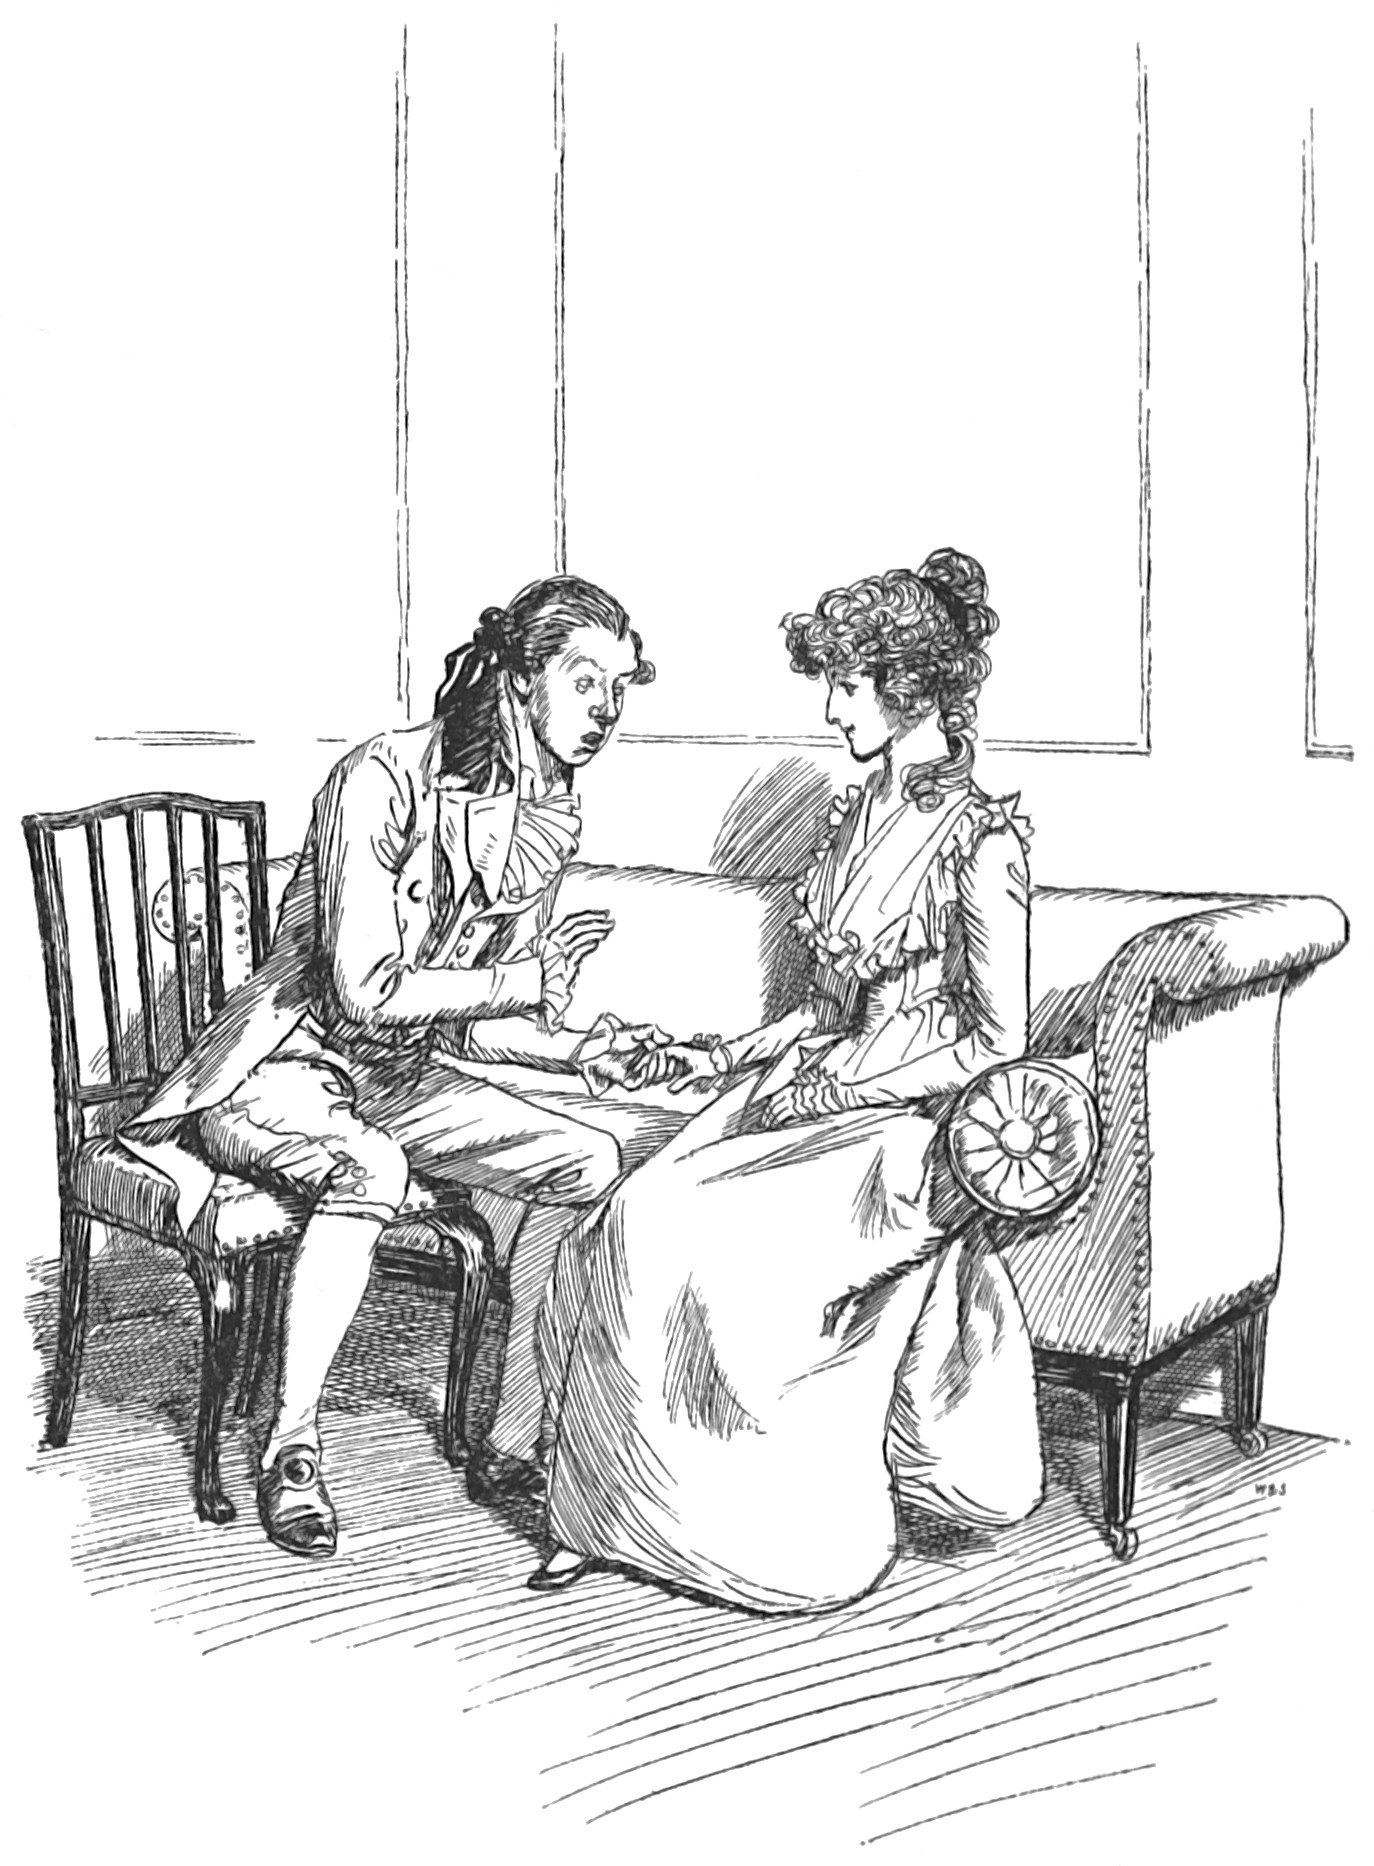
\includegraphics[width=\linewidth]{41assure}
\caption{<Of \textit{one} thing, I may assure you>}
\end{figure}

Elinor had heard enough, if not to gratify her vanity, and raise her self-importance, to agitate her nerves and fill her mind;—and she was therefore glad to be spared from the necessity of saying much in reply herself, and from the danger of hearing any thing more from her brother, by the entrance of Mr Robert Ferrars. After a few moments' chat, John Dashwood, recollecting that Fanny was yet uninformed of her sister's being there, quitted the room in quest of her; and Elinor was left to improve her acquaintance with Robert, who, by the gay unconcern, the happy self-complacency of his manner while enjoying so unfair a division of his mother's love and liberality, to the prejudice of his banished brother, earned only by his own dissipated course of life, and that brother's integrity, was confirming her most unfavourable opinion of his head and heart.

They had scarcely been two minutes by themselves, before he began to speak of Edward; for he, too, had heard of the living, and was very inquisitive on the subject. Elinor repeated the particulars of it, as she had given them to John; and their effect on Robert, though very different, was not less striking than it had been on \textit{him}. He laughed most immoderately. The idea of Edward's being a clergyman, and living in a small parsonage-house, diverted him beyond measure;—and when to that was added the fanciful imagery of Edward reading prayers in a white surplice, and publishing the banns of marriage between John Smith and Mary Brown, he could conceive nothing more ridiculous.

Elinor, while she waited in silence and immovable gravity, the conclusion of such folly, could not restrain her eyes from being fixed on him with a look that spoke all the contempt it excited. It was a look, however, very well bestowed, for it relieved her own feelings, and gave no intelligence to him. He was recalled from wit to wisdom, not by any reproof of hers, but by his own sensibility.

<We may treat it as a joke,> said he, at last, recovering from the affected laugh which had considerably lengthened out the genuine gaiety of the moment; <but, upon my soul, it is a most serious business. Poor Edward! he is ruined for ever. I am extremely sorry for it; for I know him to be a very good-hearted creature; as well-meaning a fellow perhaps, as any in the world. You must not judge of him, Miss Dashwood, from \textit{your} slight acquaintance. Poor Edward! His manners are certainly not the happiest in nature. But we are not all born, you know, with the same powers,—the same address. Poor fellow! to see him in a circle of strangers! To be sure it was pitiable enough; but upon my soul, I believe he has as good a heart as any in the kingdom; and I declare and protest to you I never was so shocked in my life, as when it all burst forth. I could not believe it. My mother was the first person who told me of it; and I, feeling myself called on to act with resolution, immediately said to her, <My dear madam, I do not know what you may intend to do on the occasion, but as for myself, I must say, that if Edward does marry this young woman, \textit{I} never will see him again.> That was what I said immediately. I was most uncommonly shocked, indeed! Poor Edward! he has done for himself completely,—shut himself out for ever from all decent society! But, as I directly said to my mother, I am not in the least surprised at it; from his style of education, it was always to be expected. My poor mother was half frantic.>

<Have you ever seen the lady?>

<Yes; once, while she was staying in this house, I happened to drop in for ten minutes; and I saw quite enough of her. The merest awkward country girl, without style, or elegance, and almost without beauty. I remember her perfectly. Just the kind of girl I should suppose likely to captivate poor Edward. I offered immediately, as soon as my mother related the affair to me, to talk to him myself, and dissuade him from the match; but it was too late \textit{then}, I found, to do any thing, for unluckily, I was not in the way at first, and knew nothing of it till after the breach had taken place, when it was not for me, you know, to interfere. But had I been informed of it a few hours earlier, I think it is most probable that something might have been hit on. I certainly should have represented it to Edward in a very strong light. <My dear fellow,> I should have said, <consider what you are doing. You are making a most disgraceful connection, and such a one as your family are unanimous in disapproving.> I cannot help thinking, in short, that means might have been found. But now it is all too late. He must be starved, you know, that is certain; absolutely starved.>

He had just settled this point with great composure, when the entrance of Mrs John Dashwood put an end to the subject. But though \textit{she} never spoke of it out of her own family, Elinor could see its influence on her mind, in the something like confusion of countenance with which she entered, and an attempt at cordiality in her behaviour to herself. She even proceeded so far as to be concerned to find that Elinor and her sister were so soon to leave town, as she had hoped to see more of them;—an exertion in which her husband, who attended her into the room, and hung enamoured over her accents, seemed to distinguish every thing that was most affectionate and graceful.
%!TeX root=../sensetop.tex
\chapter[Chapter \thechapter]{}
\lettrine[lines=4,lraise=0.3]{O}{ne} other short call in Harley Street, in which Elinor received her brother’s congratulations on their travelling so far towards Barton without any expense, and on Colonel Brandon’s being to follow them to Cleveland in a day or two, completed the intercourse of the brother and sisters in town;—and a faint invitation from Fanny, to come to Norland whenever it should happen to be in their way, which of all things was the most unlikely to occur, with a more warm, though less public, assurance, from John to Elinor, of the promptitude with which he should come to see her at Delaford, was all that foretold any meeting in the country.

It amused her to observe that all her friends seemed determined to send her to Delaford;—a place, in which, of all others, she would now least chuse to visit, or wish to reside; for not only was it considered as her future home by her brother and Mrs Jennings, but even Lucy, when they parted, gave her a pressing invitation to visit her there.

Very early in April, and tolerably early in the day, the two parties from Hanover Square and Berkeley Street set out from their respective homes, to meet, by appointment, on the road. For the convenience of Charlotte and her child, they were to be more than two days on their journey, and Mr Palmer, travelling more expeditiously with Colonel Brandon, was to join them at Cleveland soon after their arrival.

Marianne, few as had been her hours of comfort in London, and eager as she had long been to quit it, could not, when it came to the point, bid adieu to the house in which she had for the last time enjoyed those hopes, and that confidence, in Willoughby, which were now extinguished for ever, without great pain. Nor could she leave the place in which Willoughby remained, busy in new engagements, and new schemes, in which \textit{she} could have no share, without shedding many tears.

Elinor’s satisfaction, at the moment of removal, was more positive. She had no such object for her lingering thoughts to fix on, she left no creature behind, from whom it would give her a moment’s regret to be divided for ever, she was pleased to be free herself from the persecution of Lucy’s friendship, she was grateful for bringing her sister away unseen by Willoughby since his marriage, and she looked forward with hope to what a few months of tranquility at Barton might do towards restoring Marianne’s peace of mind, and confirming her own.

Their journey was safely performed. The second day brought them into the cherished, or the prohibited, county of Somerset, for as such was it dwelt on by turns in Marianne’s imagination; and in the forenoon of the third they drove up to Cleveland.

Cleveland was a spacious, modern-built house, situated on a sloping lawn. It had no park, but the pleasure-grounds were tolerably extensive; and like every other place of the same degree of importance, it had its open shrubbery, and closer wood walk, a road of smooth gravel winding round a plantation, led to the front, the lawn was dotted over with timber, the house itself was under the guardianship of the fir, the mountain-ash, and the acacia, and a thick screen of them altogether, interspersed with tall Lombardy poplars, shut out the offices.

Marianne entered the house with a heart swelling with emotion from the consciousness of being only eighty miles from Barton, and not thirty from Combe Magna; and before she had been five minutes within its walls, while the others were busily helping Charlotte to show her child to the housekeeper, she quitted it again, stealing away through the winding shrubberies, now just beginning to be in beauty, to gain a distant eminence; where, from its Grecian temple, her eye, wandering over a wide tract of country to the south-east, could fondly rest on the farthest ridge of hills in the horizon, and fancy that from their summits Combe Magna might be seen.

\begin{figure}[tbph]
\centering
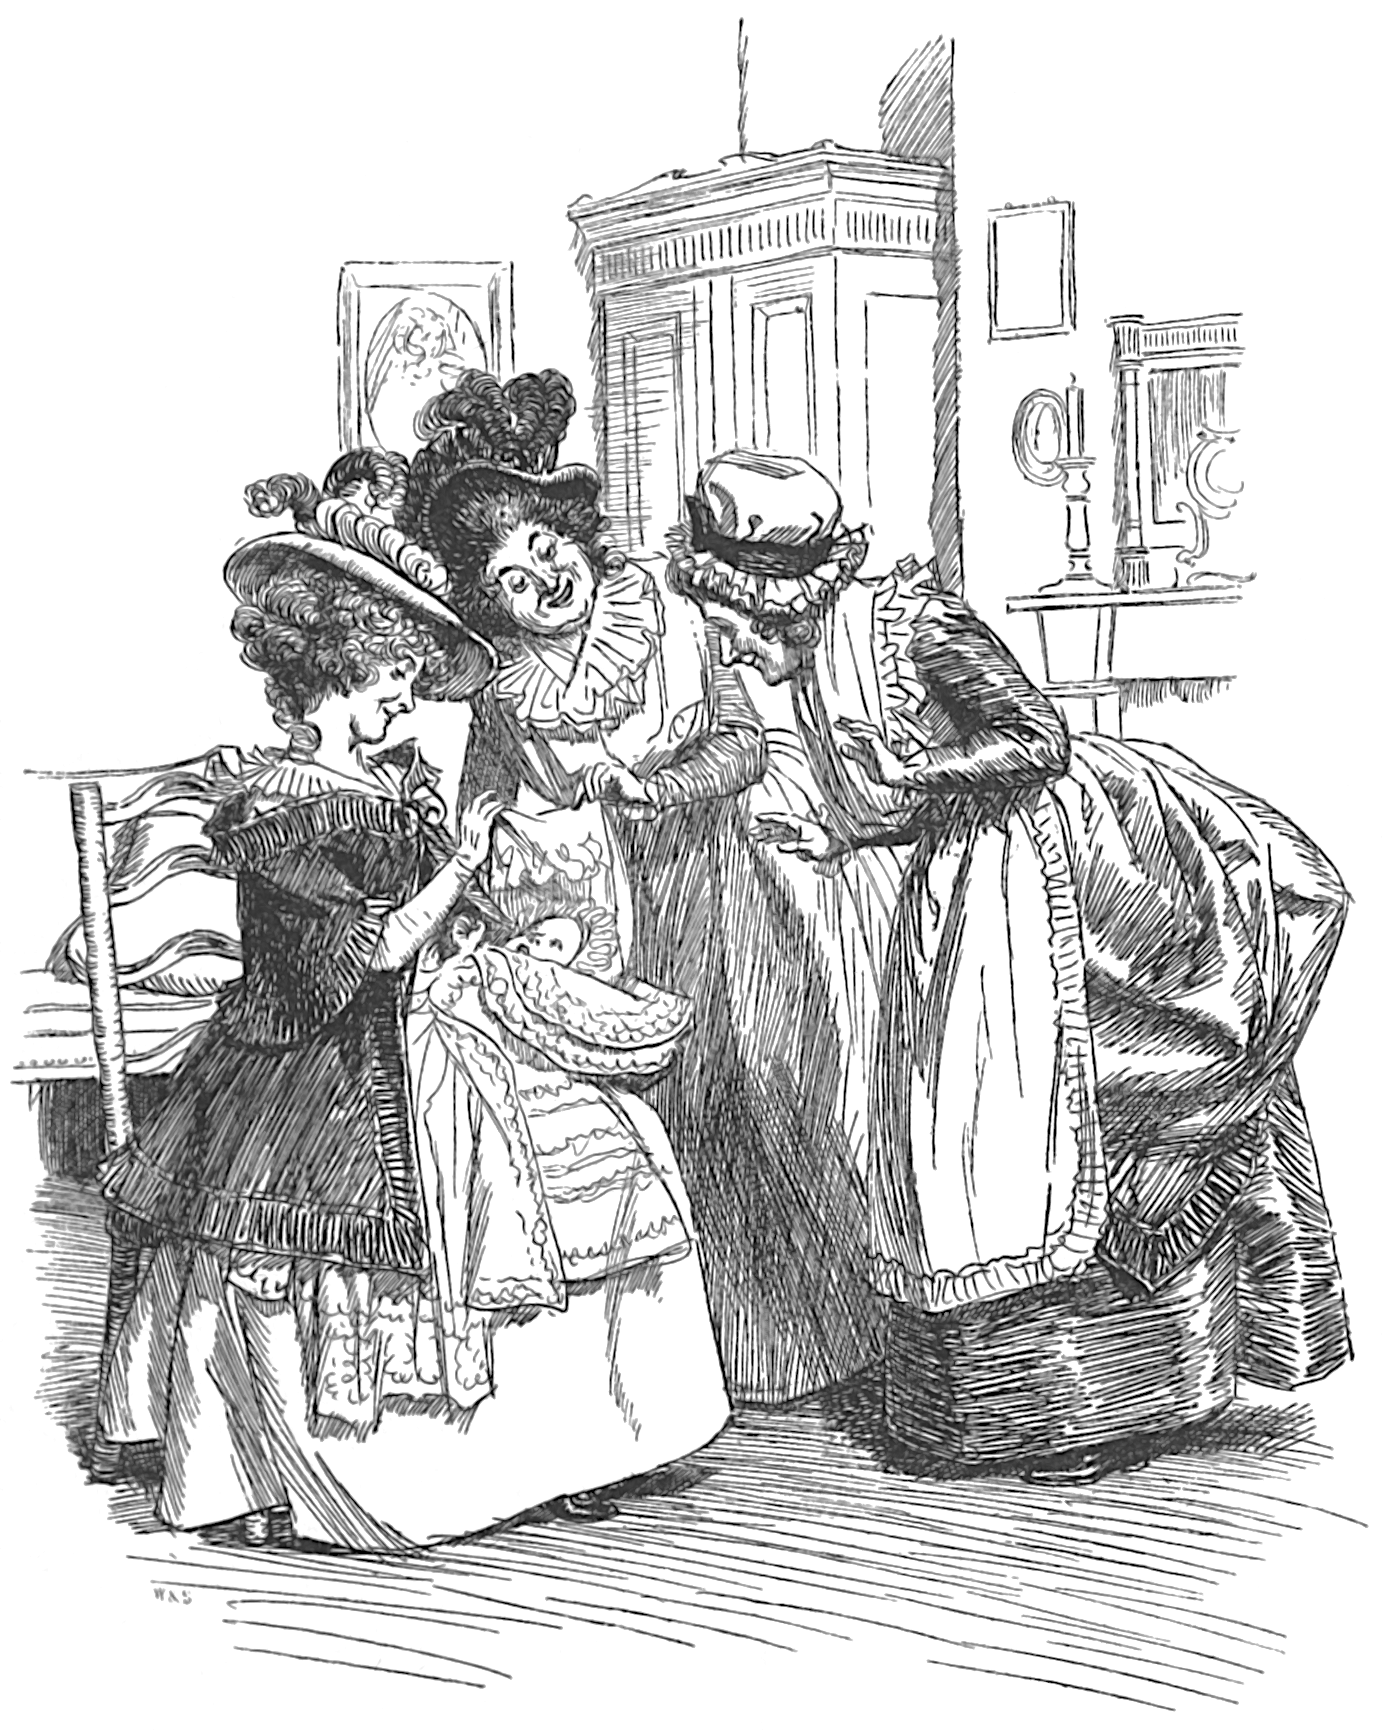
\includegraphics[width=\linewidth]{42child}
\caption{Show her child to the housekeeper}
\end{figure}

In such moments of precious, invaluable misery, she rejoiced in tears of agony to be at Cleveland; and as she returned by a different circuit to the house, feeling all the happy privilege of country liberty, of wandering from place to place in free and luxurious solitude, she resolved to spend almost every hour of every day while she remained with the Palmers, in the indulgence of such solitary rambles.

She returned just in time to join the others as they quitted the house, on an excursion through its more immediate premises; and the rest of the morning was easily whiled away, in lounging round the kitchen garden, examining the bloom upon its walls, and listening to the gardener’s lamentations upon blights, in dawdling through the green-house, where the loss of her favourite plants, unwarily exposed, and nipped by the lingering frost, raised the laughter of Charlotte,—and in visiting her poultry-yard, where, in the disappointed hopes of her dairy-maid, by hens forsaking their nests, or being stolen by a fox, or in the rapid decrease of a promising young brood, she found fresh sources of merriment.



\makeatletter
\@ifclasswith{scrbook}{a5paper}
{%
\begin{figure}[tbph]
	\centering
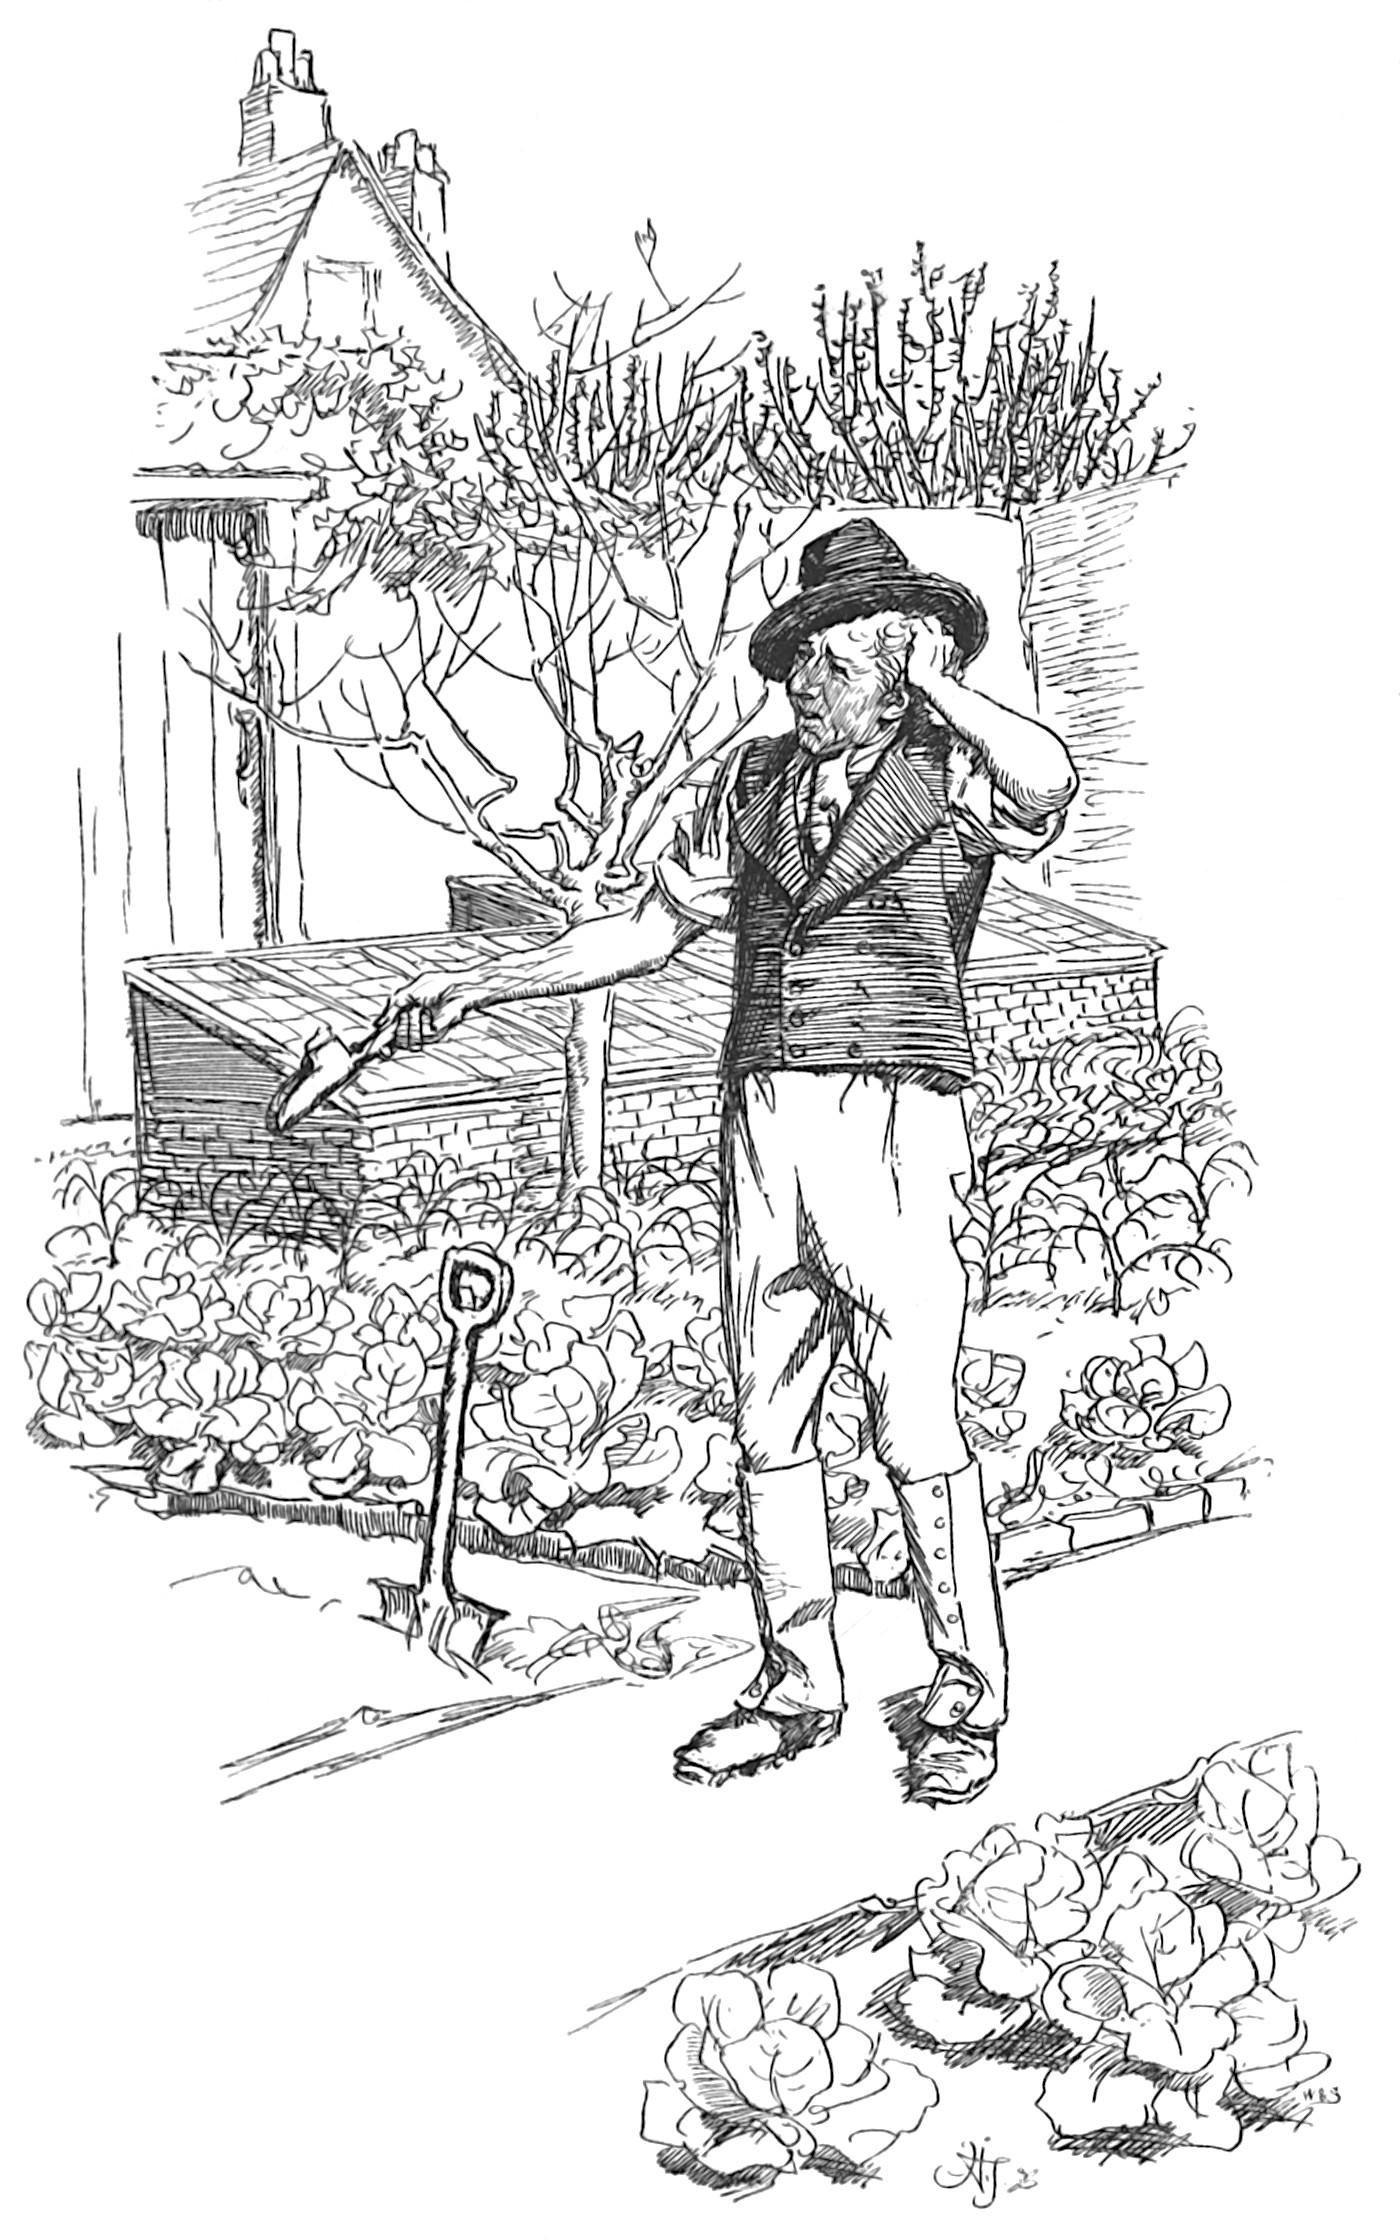
\includegraphics[width=.9\linewidth]{42lament}
\caption{The gardener’s lamentations}
\end{figure}
}{%
\begin{figure}[tbph]
\centering
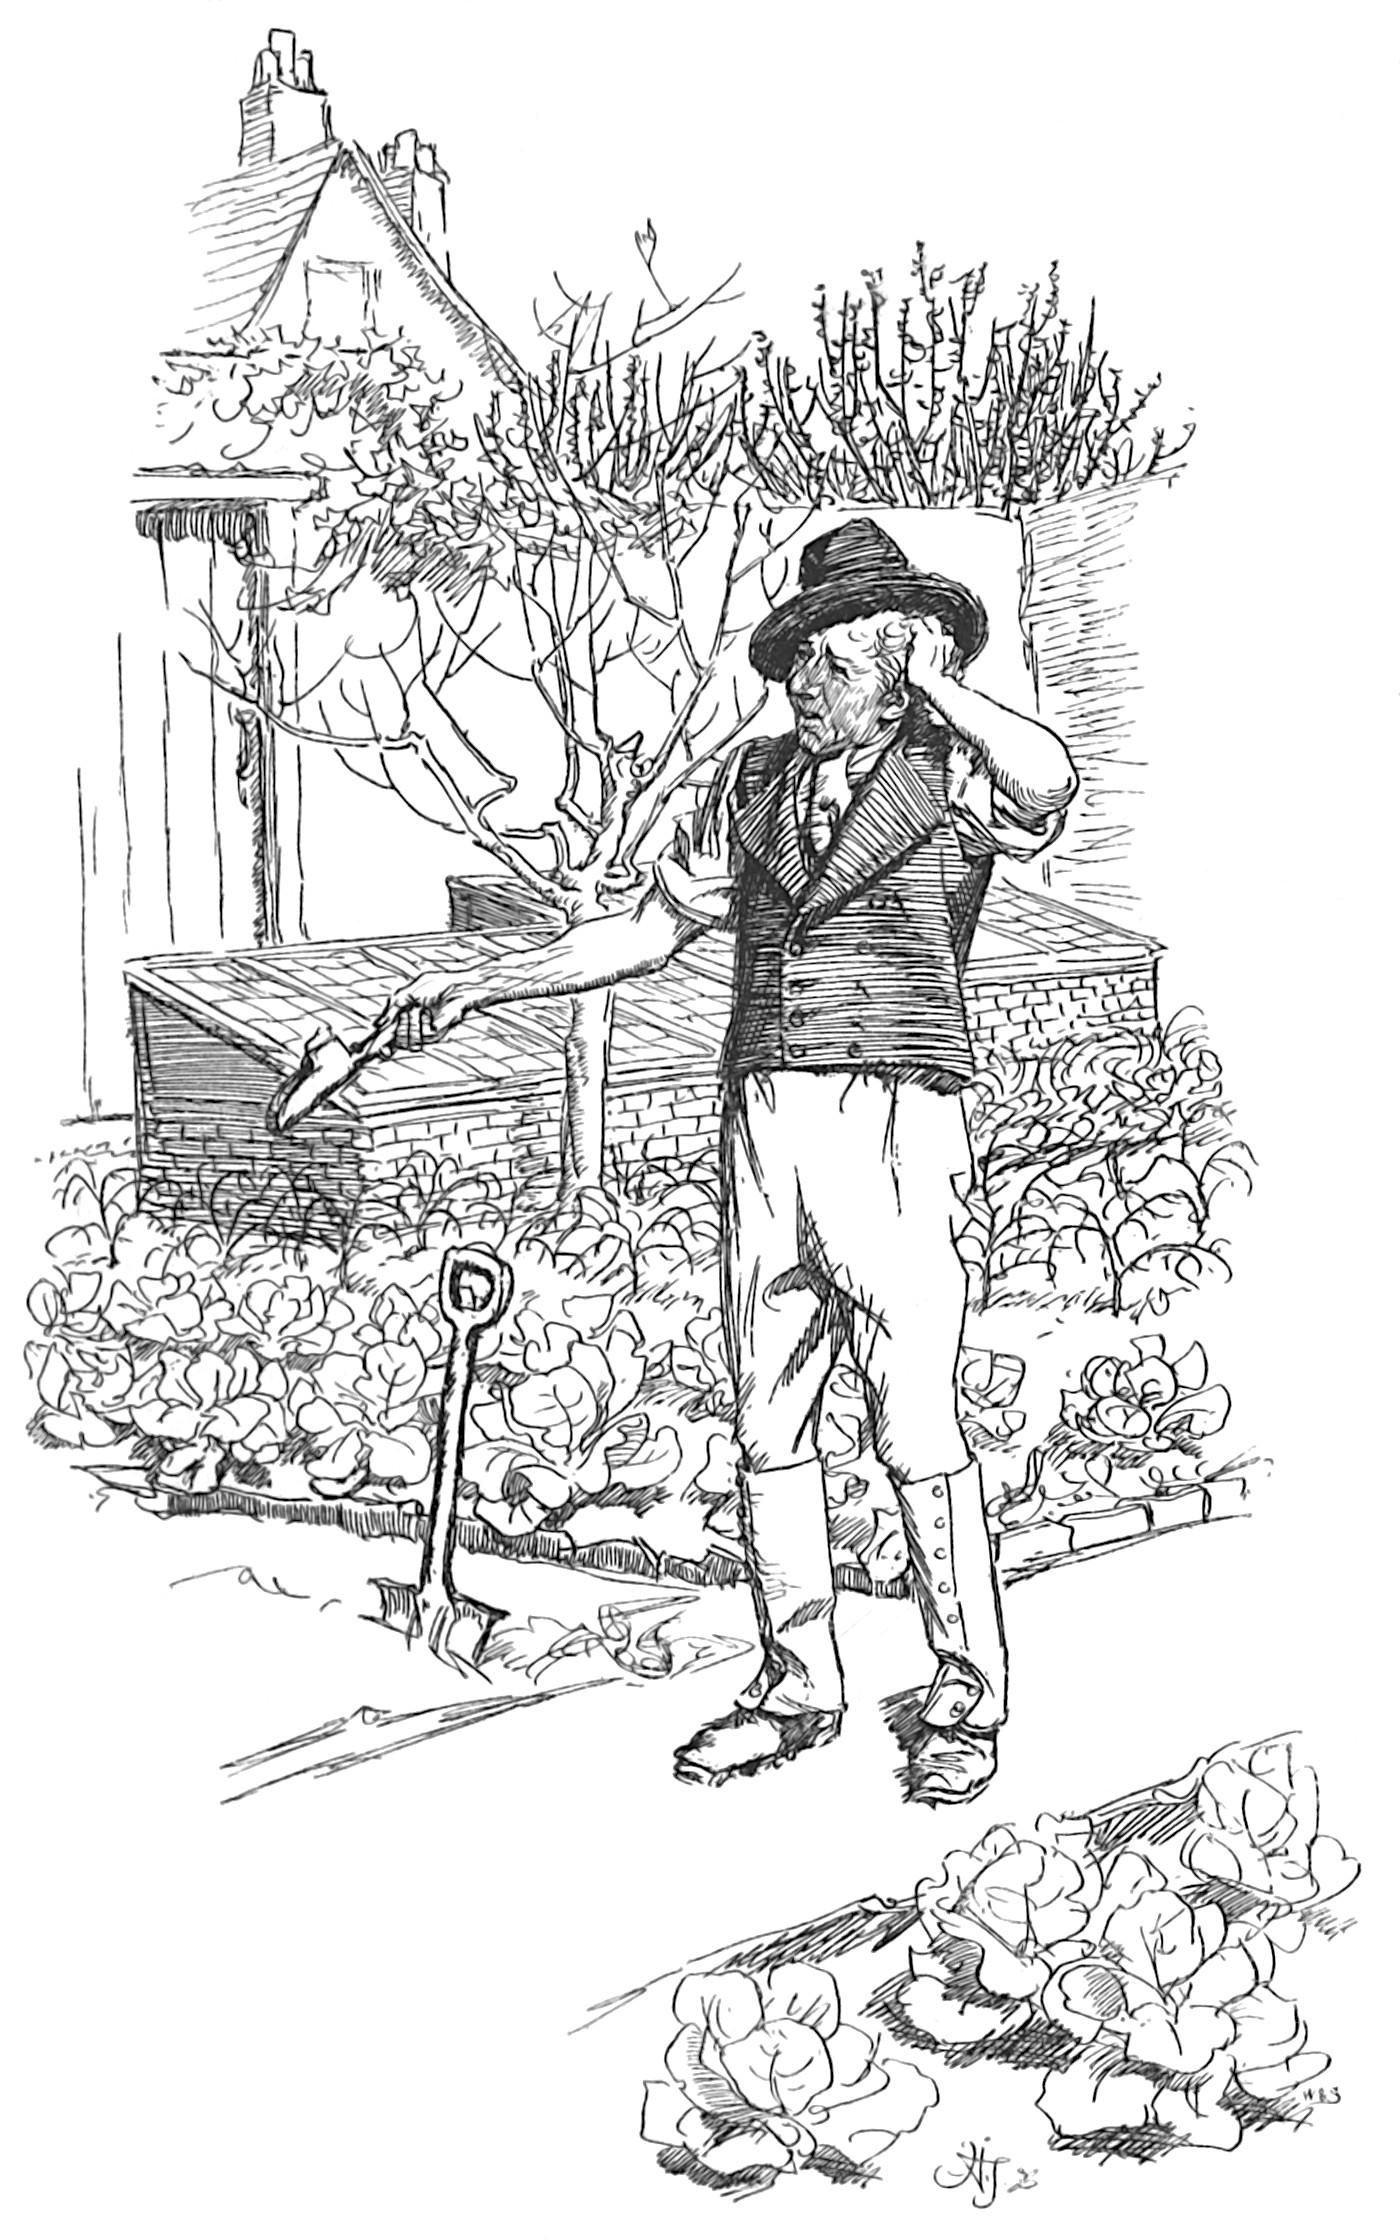
\includegraphics[width=\linewidth]{42lament}
\caption{The gardener’s lamentations}
\end{figure}
}
\makeatother


The morning was fine and dry, and Marianne, in her plan of employment abroad, had not calculated for any change of weather during their stay at Cleveland. With great surprise therefore, did she find herself prevented by a settled rain from going out again after dinner. She had depended on a twilight walk to the Grecian temple, and perhaps all over the grounds, and an evening merely cold or damp would not have deterred her from it; but a heavy and settled rain even \textit{she} could not fancy dry or pleasant weather for walking.

Their party was small, and the hours passed quietly away. Mrs Palmer had her child, and Mrs Jennings her carpet-work; they talked of the friends they had left behind, arranged Lady Middleton’s engagements, and wondered whether Mr Palmer and Colonel Brandon would get farther than Reading that night. Elinor, however little concerned in it, joined in their discourse; and Marianne, who had the knack of finding her way in every house to the library, however it might be avoided by the family in general, soon procured herself a book.

Nothing was wanting on Mrs Palmer’s side that constant and friendly good humour could do, to make them feel themselves welcome. The openness and heartiness of her manner more than atoned for that want of recollection and elegance which made her often deficient in the forms of politeness; her kindness, recommended by so pretty a face, was engaging; her folly, though evident was not disgusting, because it was not conceited; and Elinor could have forgiven every thing but her laugh.

The two gentlemen arrived the next day to a very late dinner, affording a pleasant enlargement of the party, and a very welcome variety to their conversation, which a long morning of the same continued rain had reduced very low.

Elinor had seen so little of Mr Palmer, and in that little had seen so much variety in his address to her sister and herself, that she knew not what to expect to find him in his own family. She found him, however, perfectly the gentleman in his behaviour to all his visitors, and only occasionally rude to his wife and her mother; she found him very capable of being a pleasant companion, and only prevented from being so always, by too great an aptitude to fancy himself as much superior to people in general, as he must feel himself to be to Mrs Jennings and Charlotte. For the rest of his character and habits, they were marked, as far as Elinor could perceive, with no traits at all unusual in his sex and time of life. He was nice in his eating, uncertain in his hours; fond of his child, though affecting to slight it; and idled away the mornings at billiards, which ought to have been devoted to business. She liked him, however, upon the whole, much better than she had expected, and in her heart was not sorry that she could like him no more;—not sorry to be driven by the observation of his Epicurism, his selfishness, and his conceit, to rest with complacency on the remembrance of Edward’s generous temper, simple taste, and diffident feelings.

Of Edward, or at least of some of his concerns, she now received intelligence from Colonel Brandon, who had been into Dorsetshire lately; and who, treating her at once as the disinterested friend of Mr Ferrars, and the kind confidante of himself, talked to her a great deal of the parsonage at Delaford, described its deficiencies, and told her what he meant to do himself towards removing them.—His behaviour to her in this, as well as in every other particular, his open pleasure in meeting her after an absence of only ten days, his readiness to converse with her, and his deference for her opinion, might very well justify Mrs Jennings’s persuasion of his attachment, and would have been enough, perhaps, had not Elinor still, as from the first, believed Marianne his real favourite, to make her suspect it herself. But as it was, such a notion had scarcely ever entered her head, except by Mrs Jennings’s suggestion; and she could not help believing herself the nicest observer of the two;—she watched his eyes, while Mrs Jennings thought only of his behaviour;—and while his looks of anxious solicitude on Marianne’s feeling, in her head and throat, the beginning of a heavy cold, because unexpressed by words, entirely escaped the latter lady’s observation;—\textit{she} could discover in them the quick feelings, and needless alarm of a lover.

Two delightful twilight walks on the third and fourth evenings of her being there, not merely on the dry gravel of the shrubbery, but all over the grounds, and especially in the most distant parts of them, where there was something more of wildness than in the rest, where the trees were the oldest, and the grass was the longest and wettest, had—assisted by the still greater imprudence of sitting in her wet shoes and stockings—given Marianne a cold so violent as, though for a day or two trifled with or denied, would force itself by increasing ailments on the concern of every body, and the notice of herself. Prescriptions poured in from all quarters, and as usual, were all declined. Though heavy and feverish, with a pain in her limbs, and a cough, and a sore throat, a good night’s rest was to cure her entirely; and it was with difficulty that Elinor prevailed on her, when she went to bed, to try one or two of the simplest of the remedies.
%!TeX root=../sensetop.tex
\chapter[Chapter \thechapter]{}
\lettrine[lines=4,lraise=0.3]{M}{arianne} got up the next morning at her usual time; to every inquiry replied that she was better, and tried to prove herself so, by engaging in her accustomary employments. But a day spent in sitting shivering over the fire with a book in her hand, which she was unable to read, or in lying, weary and languid, on a sofa, did not speak much in favour of her amendment; and when, at last, she went early to bed, more and more indisposed, Colonel Brandon was only astonished at her sister’s composure, who, though attending and nursing her the whole day, against Marianne’s inclination, and forcing proper medicines on her at night, trusted, like Marianne, to the certainty and efficacy of sleep, and felt no real alarm.

A very restless and feverish night, however, disappointed the expectation of both; and when Marianne, after persisting in rising, confessed herself unable to sit up, and returned voluntarily to her bed, Elinor was very ready to adopt Mrs Jennings’s advice, of sending for the Palmers’ apothecary.

He came, examined his patient, and though encouraging Miss Dashwood to expect that a very few days would restore her sister to health, yet, by pronouncing her disorder to have a putrid tendency, and allowing the word »infection« to pass his lips, gave instant alarm to Mrs Palmer, on her baby’s account. Mrs Jennings, who had been inclined from the first to think Marianne’s complaint more serious than Elinor, now looked very grave on Mr Harris’s report, and confirming Charlotte’s fears and caution, urged the necessity of her immediate removal with her infant; and Mr Palmer, though treating their apprehensions as idle, found the anxiety and importunity of his wife too great to be withstood. Her departure, therefore, was fixed on; and within an hour after Mr Harris’s arrival, she set off, with her little boy and his nurse, for the house of a near relation of Mr Palmer’s, who lived a few miles on the other side of Bath; whither her husband promised, at her earnest entreaty, to join her in a day or two; and whither she was almost equally urgent with her mother to accompany her. Mrs Jennings, however, with a kindness of heart which made Elinor really love her, declared her resolution of not stirring from Cleveland as long as Marianne remained ill, and of endeavouring, by her own attentive care, to supply to her the place of the mother she had taken her from; and Elinor found her on every occasion a most willing and active helpmate, desirous to share in all her fatigues, and often by her better experience in nursing, of material use.

Poor Marianne, languid and low from the nature of her malady, and feeling herself universally ill, could no longer hope that tomorrow would find her recovered; and the idea of what tomorrow would have produced, but for this unlucky illness, made every ailment severe; for on that day they were to have begun their journey home; and, attended the whole way by a servant of Mrs Jennings, were to have taken their mother by surprise on the following forenoon. The little she said was all in lamentation of this inevitable delay; though Elinor tried to raise her spirits, and make her believe, as she \textit{then} really believed herself, that it would be a very short one.

The next day produced little or no alteration in the state of the patient; she certainly was not better, and, except that there was no amendment, did not appear worse. Their party was now farther reduced; for Mr Palmer, though very unwilling to go as well from real humanity and good-nature, as from a dislike of appearing to be frightened away by his wife, was persuaded at last by Colonel Brandon to perform his promise of following her; and while he was preparing to go, Colonel Brandon himself, with a much greater exertion, began to talk of going likewise.—Here, however, the kindness of Mrs Jennings interposed most acceptably; for to send the Colonel away while his love was in so much uneasiness on her sister’s account, would be to deprive them both, she thought, of every comfort; and therefore telling him at once that his stay at Cleveland was necessary to herself, that she should want him to play at piquet of an evening, while Miss Dashwood was above with her sister, \&c. she urged him so strongly to remain, that he, who was gratifying the first wish of his own heart by a compliance, could not long even affect to demur; especially as Mrs Jennings’s entreaty was warmly seconded by Mr Palmer, who seemed to feel a relief to himself, in leaving behind him a person so well able to assist or advise Miss Dashwood in any emergence.

Marianne was, of course, kept in ignorance of all these arrangements. She knew not that she had been the means of sending the owners of Cleveland away, in about seven days from the time of their arrival. It gave her no surprise that she saw nothing of Mrs Palmer; and as it gave her likewise no concern, she never mentioned her name.

Two days passed away from the time of Mr Palmer’s departure, and her situation continued, with little variation, the same. Mr Harris, who attended her every day, still talked boldly of a speedy recovery, and Miss Dashwood was equally sanguine; but the expectation of the others was by no means so cheerful. Mrs Jennings had determined very early in the seizure that Marianne would never get over it, and Colonel Brandon, who was chiefly of use in listening to Mrs Jennings’s forebodings, was not in a state of mind to resist their influence. He tried to reason himself out of fears, which the different judgment of the apothecary seemed to render absurd; but the many hours of each day in which he was left entirely alone, were but too favourable for the admission of every melancholy idea, and he could not expel from his mind the persuasion that he should see Marianne no more.

On the morning of the third day however, the gloomy anticipations of both were almost done away; for when Mr Harris arrived, he declared his patient materially better. Her pulse was much stronger, and every symptom more favourable than on the preceding visit. Elinor, confirmed in every pleasant hope, was all cheerfulness; rejoicing that in her letters to her mother, she had pursued her own judgment rather than her friend’s, in making very light of the indisposition which delayed them at Cleveland; and almost fixing on the time when Marianne would be able to travel.

But the day did not close so auspiciously as it began. Towards the evening Marianne became ill again, growing more heavy, restless, and uncomfortable than before. Her sister, however, still sanguine, was willing to attribute the change to nothing more than the fatigue of having sat up to have her bed made; and carefully administering the cordials prescribed, saw her, with satisfaction, sink at last into a slumber, from which she expected the most beneficial effects. Her sleep, though not so quiet as Elinor wished to see it, lasted a considerable time; and anxious to observe the result of it herself, she resolved to sit with her during the whole of it. Mrs Jennings, knowing nothing of any change in the patient, went unusually early to bed; her maid, who was one of the principal nurses, was recreating herself in the housekeeper’s room, and Elinor remained alone with Marianne.

The repose of the latter became more and more disturbed; and her sister, who watched, with unremitting attention her continual change of posture, and heard the frequent but inarticulate sounds of complaint which passed her lips, was almost wishing to rouse her from so painful a slumber, when Marianne, suddenly awakened by some accidental noise in the house, started hastily up, and, with feverish wildness, cried out,—

»Is mama coming?«

»Not yet,« cried the other, concealing her terror, and assisting Marianne to lie down again, »but she will be here, I hope, before it is long. It is a great way, you know, from hence to Barton.«

»But she must not go round by London,« cried Marianne, in the same hurried manner. »I shall never see her, if she goes by London.«

Elinor perceived with alarm that she was not quite herself, and, while attempting to soothe her, eagerly felt her pulse. It was lower and quicker than ever! and Marianne, still talking wildly of mama, her alarm increased so rapidly, as to determine her on sending instantly for Mr Harris, and despatching a messenger to Barton for her mother. To consult with Colonel Brandon on the best means of effecting the latter, was a thought which immediately followed the resolution of its performance; and as soon she had rung up the maid to take her place by her sister, she hastened down to the drawing-room, where she knew he was generally to be found at a much later hour than the present.

It was no time for hesitation. Her fears and her difficulties were immediately before him. Her fears, he had no courage, no confidence to attempt the removal of:—he listened to them in silent despondence;—but her difficulties were instantly obviated, for with a readiness that seemed to speak the occasion, and the service pre-arranged in his mind, he offered himself as the messenger who should fetch Mrs Dashwood. Elinor made no resistance that was not easily overcome. She thanked him with brief, though fervent gratitude, and while he went to hurry off his servant with a message to Mr Harris, and an order for post-horses directly, she wrote a few lines to her mother.

The comfort of such a friend at that moment as Colonel Brandon—or such a companion for her mother,—how gratefully was it felt!—a companion whose judgment would guide, whose attendance must relieve, and whose friendship might soothe her!—as far as the shock of such a summons \textit{could} be lessened to her, his presence, his manners, his assistance, would lessen it.

\textit{He}, meanwhile, whatever he might feel, acted with all the firmness of a collected mind, made every necessary arrangement with the utmost despatch, and calculated with exactness the time in which she might look for his return. Not a moment was lost in delay of any kind. The horses arrived, even before they were expected, and Colonel Brandon only pressing her hand with a look of solemnity, and a few words spoken too low to reach her ear, hurried into the carriage. It was then about twelve o’clock, and she returned to her sister’s apartment to wait for the arrival of the apothecary, and to watch by her the rest of the night. It was a night of almost equal suffering to both. Hour after hour passed away in sleepless pain and delirium on Marianne’s side, and in the most cruel anxiety on Elinor’s, before Mr Harris appeared. Her apprehensions once raised, paid by their excess for all her former security; and the servant who sat up with her, for she would not allow Mrs Jennings to be called, only tortured her more, by hints of what her mistress had always thought.

Marianne’s ideas were still, at intervals, fixed incoherently on her mother, and whenever she mentioned her name, it gave a pang to the heart of poor Elinor, who, reproaching herself for having trifled with so many days of illness, and wretched for some immediate relief, fancied that all relief might soon be in vain, that every thing had been delayed too long, and pictured to herself her suffering mother arriving too late to see this darling child, or to see her rational.

She was on the point of sending again for Mr Harris, or if \textit{he} could not come, for some other advice, when the former—but not till after five o’clock—arrived. His opinion, however, made some little amends for his delay, for though acknowledging a very unexpected and unpleasant alteration in his patient, he would not allow the danger to be material, and talked of the relief which a fresh mode of treatment must procure, with a confidence which, in a lesser degree, was communicated to Elinor. He promised to call again in the course of three or four hours, and left both the patient and her anxious attendant more composed than he had found them.

With strong concern, and with many reproaches for not being called to their aid, did Mrs Jennings hear in the morning of what had passed. Her former apprehensions, now with greater reason restored, left her no doubt of the event; and though trying to speak comfort to Elinor, her conviction of her sister’s danger would not allow her to offer the comfort of hope. Her heart was really grieved. The rapid decay, the early death of a girl so young, so lovely as Marianne, must have struck a less interested person with concern. On Mrs Jennings’s compassion she had other claims. She had been for three months her companion, was still under her care, and she was known to have been greatly injured, and long unhappy. The distress of her sister too, particularly a favourite, was before her;—and as for their mother, when Mrs Jennings considered that Marianne might probably be to \textit{her} what Charlotte was to herself, her sympathy in \textit{her} sufferings was very sincere.

Mr Harris was punctual in his second visit;—but he came to be disappointed in his hopes of what the last would produce. His medicines had failed;—the fever was unabated; and Marianne only more quiet—not more herself—remained in a heavy stupor. Elinor, catching all, and more than all, his fears in a moment, proposed to call in further advice. But he judged it unnecessary: he had still something more to try, some more fresh application, of whose success he was as confident as the last, and his visit concluded with encouraging assurances which reached the ear, but could not enter the heart of Miss Dashwood. She was calm, except when she thought of her mother; but she was almost hopeless; and in this state she continued till noon, scarcely stirring from her sister’s bed, her thoughts wandering from one image of grief, one suffering friend to another, and her spirits oppressed to the utmost by the conversation of Mrs Jennings, who scrupled not to attribute the severity and danger of this attack to the many weeks of previous indisposition which Marianne’s disappointment had brought on. Elinor felt all the reasonableness of the idea, and it gave fresh misery to her reflections.

About noon, however, she began—but with a caution—a dread of disappointment which for some time kept her silent, even to her friend—to fancy, to hope she could perceive a slight amendment in her sister’s pulse;—she waited, watched, and examined it again and again;—and at last, with an agitation more difficult to bury under exterior calmness, than all her foregoing distress, ventured to communicate her hopes. Mrs Jennings, though forced, on examination, to acknowledge a temporary revival, tried to keep her young friend from indulging a thought of its continuance;—and Elinor, conning over every injunction of distrust, told herself likewise not to hope. But it was too late. Hope had already entered; and feeling all its anxious flutter, she bent over her sister to watch—she hardly knew for what. Half an hour passed away, and the favourable symptom yet blessed her. Others even arose to confirm it. Her breath, her skin, her lips, all flattered Elinor with signs of amendment; and Marianne fixed her eyes on her with a rational, though languid, gaze. Anxiety and hope now oppressed her in equal degrees, and left her no moment of tranquillity till the arrival of Mr Harris at four o’clock;—when his assurances, his felicitations on a recovery in her sister even surpassing his expectation, gave her confidence, comfort, and tears of joy.

Marianne was in every respect materially better, and he declared her entirely out of danger. Mrs Jennings, perhaps satisfied with the partial justification of her forebodings which had been found in their late alarm, allowed herself to trust in his judgment, and admitted, with unfeigned joy, and soon with unequivocal cheerfulness, the probability of an entire recovery.

Elinor could not be cheerful. Her joy was of a different kind, and led to any thing rather than to gaiety. Marianne restored to life, health, friends, and to her doting mother, was an idea to fill her heart with sensations of exquisite comfort, and expand it in fervent gratitude;—but it led to no outward demonstrations of joy, no words, no smiles. All within Elinor’s breast was satisfaction, silent and strong.

She continued by the side of her sister, with little intermission the whole afternoon, calming every fear, satisfying every inquiry of her enfeebled spirits, supplying every succour, and watching almost every look and every breath. The possibility of a relapse would of course, in some moments, occur to remind her of what anxiety was—but when she saw, on her frequent and minute examination, that every symptom of recovery continued, and saw Marianne at six o’clock sink into a quiet, steady, and to all appearance comfortable, sleep, she silenced every doubt.

The time was now drawing on, when Colonel Brandon might be expected back. At ten o’clock, she trusted, or at least not much later her mother would be relieved from the dreadful suspense in which she must now be travelling towards them. The Colonel, too!—perhaps scarcely less an object of pity!—Oh!—how slow was the progress of time which yet kept them in ignorance!

At seven o’clock, leaving Marianne still sweetly asleep, she joined Mrs Jennings in the drawing-room to tea. Of breakfast she had been kept by her fears, and of dinner by their sudden reverse, from eating much;—and the present refreshment, therefore, with such feelings of content as she brought to it, was particularly welcome. Mrs Jennings would have persuaded her, at its conclusion, to take some rest before her mother’s arrival, and allow \textit{her} to take her place by Marianne; but Elinor had no sense of fatigue, no capability of sleep at that moment about her, and she was not to be kept away from her sister an unnecessary instant. Mrs Jennings therefore attending her up stairs into the sick chamber, to satisfy herself that all continued right, left her there again to her charge and her thoughts, and retired to her own room to write letters and sleep.

The night was cold and stormy. The wind roared round the house, and the rain beat against the windows; but Elinor, all happiness within, regarded it not. Marianne slept through every blast; and the travellers—they had a rich reward in store, for every present inconvenience.

The clock struck eight. Had it been ten, Elinor would have been convinced that at that moment she heard a carriage driving up to the house; and so strong was the persuasion that she \textit{did}, in spite of the \textit{almost} impossibility of their being already come, that she moved into the adjoining dressing-closet and opened a window shutter, to be satisfied of the truth. She instantly saw that her ears had not deceived her. The flaring lamps of a carriage were immediately in view. By their uncertain light she thought she could discern it to be drawn by four horses; and this, while it told the excess of her poor mother’s alarm, gave some explanation to such unexpected rapidity.

\begin{a4}
	\begin{figure}[tbph]
		\centering
		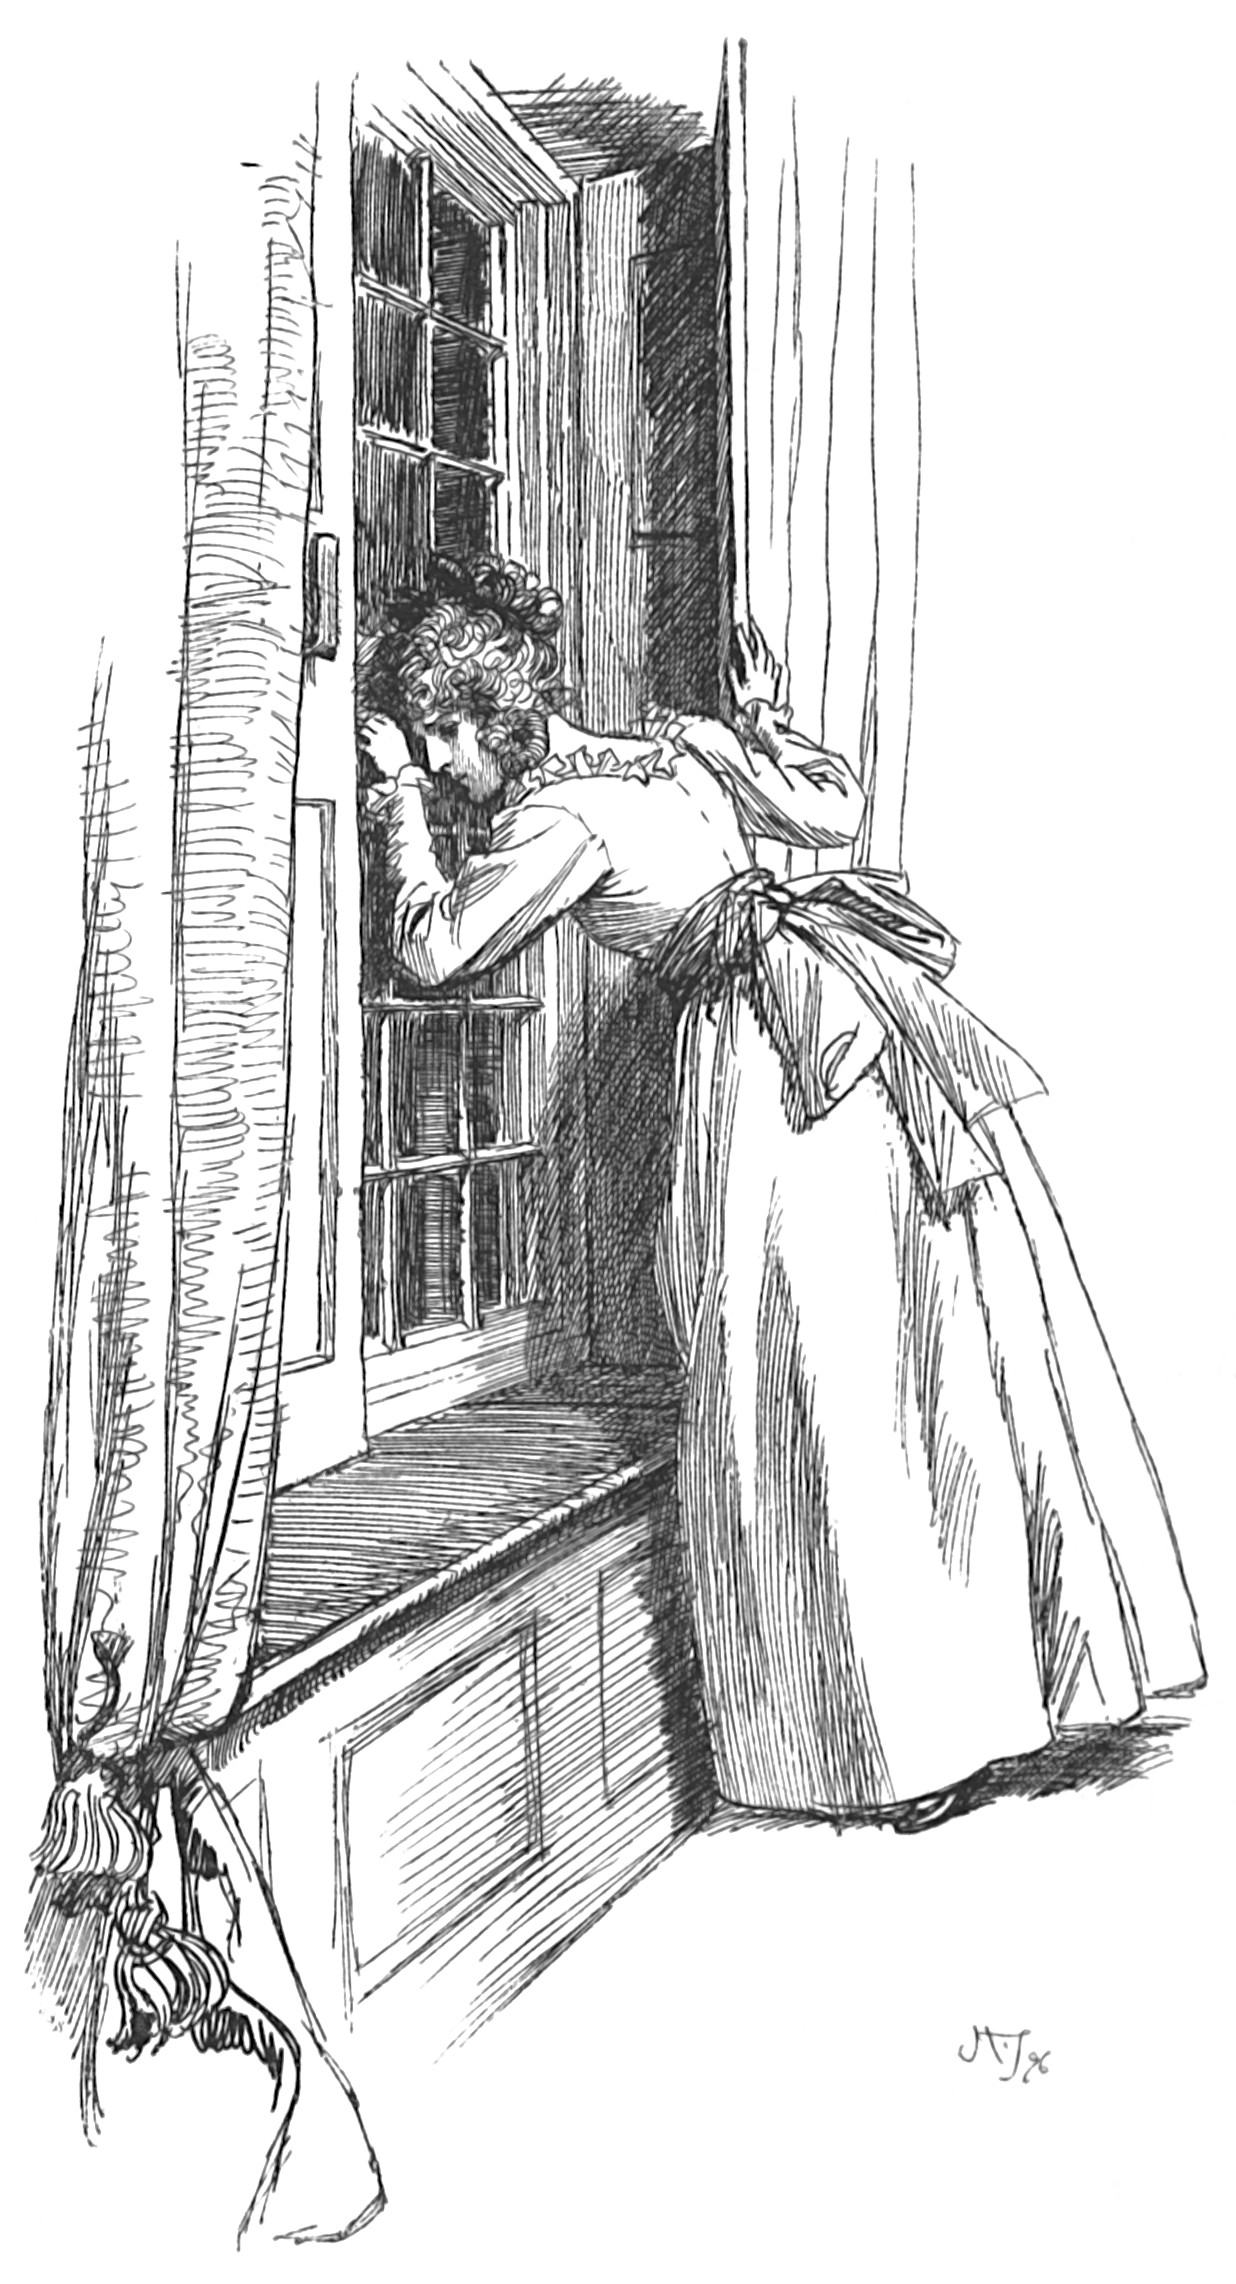
\includegraphics[width=.8\linewidth]{43shutter}
		\caption{Opened a window shutter}
	\end{figure}
\end{a4}

\begin{letter}
	\begin{figure}[tbph]
		\centering
		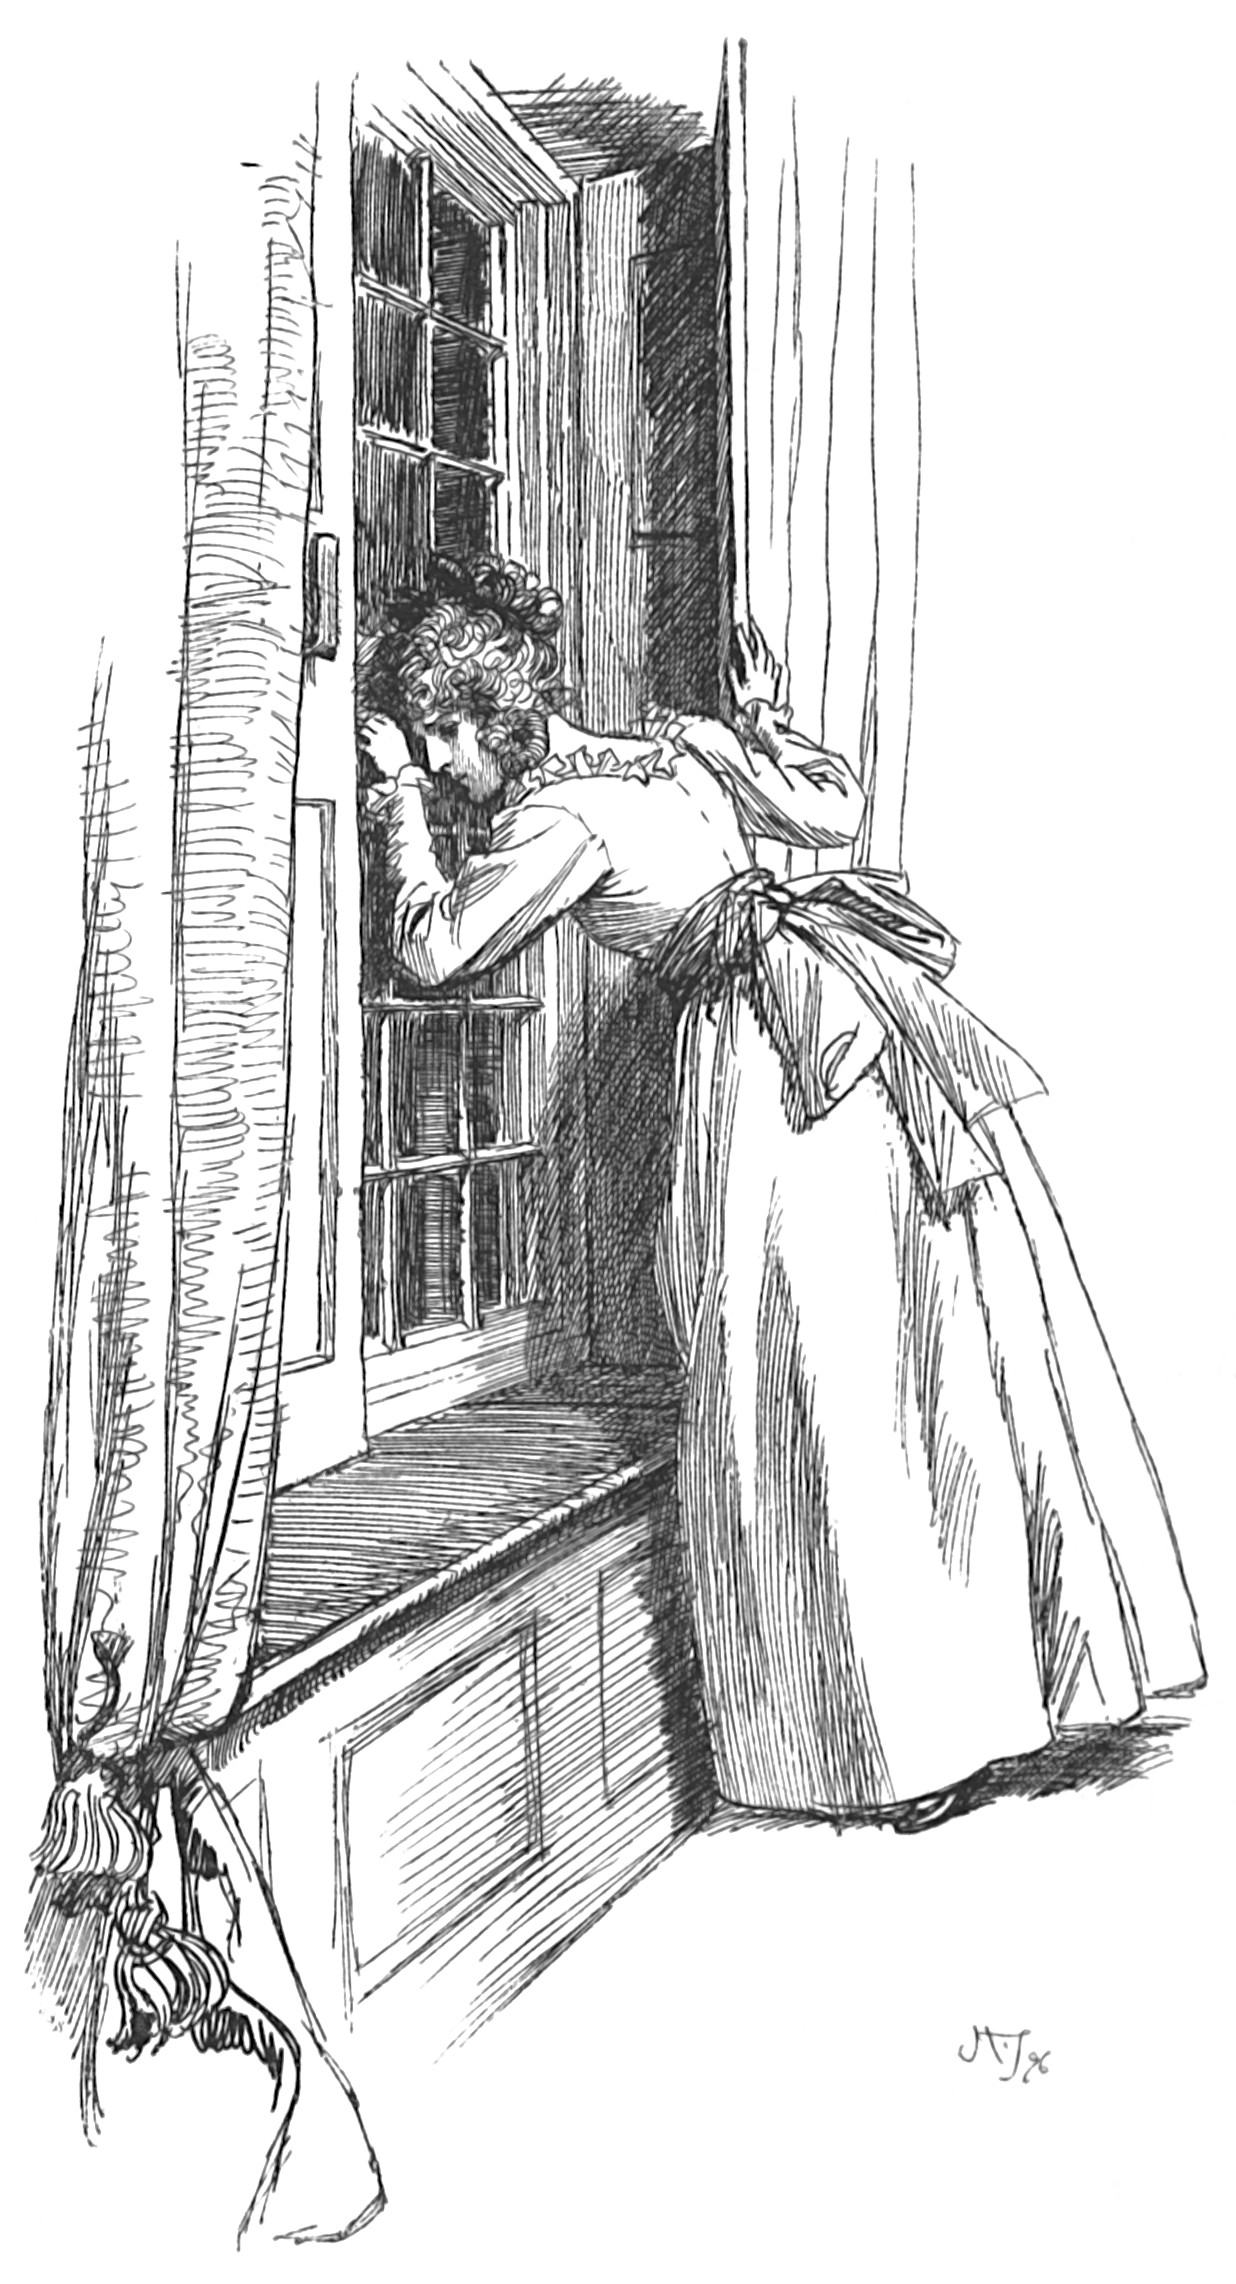
\includegraphics[width=.9\linewidth]{43shutter}
		\caption{Opened a window shutter}
	\end{figure}
\end{letter}

Never in her life had Elinor found it so difficult to be calm, as at that moment. The knowledge of what her mother must be feeling as the carriage stopt at the door—of her doubt—her dread—perhaps her despair!—and of what \textit{she} had to tell!—with such knowledge it was impossible to be calm. All that remained to be done was to be speedy; and, therefore staying only till she could leave Mrs Jennings’s maid with her sister, she hurried down stairs.

The bustle in the vestibule, as she passed along an inner lobby, assured her that they were already in the house. She rushed to the drawing-room,—she entered it,—and saw only Willoughby.
%!TeX root=../emmatop.tex
\chapter[Chapter \thechapter]{}
\lettrine[lines=4,lraise=0.3]{T}{he} wretchedness of a scheme to Box Hill was in Emma's thoughts all the evening. How it might be considered by the rest of the party, she could not tell. They, in their different homes, and their different ways, might be looking back on it with pleasure; but in her view it was a morning more completely misspent, more totally bare of rational satisfaction at the time, and more to be abhorred in recollection, than any she had ever passed. A whole evening of back-gammon with her father, was felicity to it. There, indeed, lay real pleasure, for there she was giving up the sweetest hours of the twenty-four to his comfort; and feeling that, unmerited as might be the degree of his fond affection and confiding esteem, she could not, in her general conduct, be open to any severe reproach. As a daughter, she hoped she was not without a heart. She hoped no one could have said to her, »How could you be so unfeeling to your father?—I must, I will tell you truths while I can.« Miss Bates should never again—no, never! If attention, in future, could do away the past, she might hope to be forgiven. She had been often remiss, her conscience told her so; remiss, perhaps, more in thought than fact; scornful, ungracious. But it should be so no more. In the warmth of true contrition, she would call upon her the very next morning, and it should be the beginning, on her side, of a regular, equal, kindly intercourse.

She was just as determined when the morrow came, and went early, that nothing might prevent her. It was not unlikely, she thought, that she might see Mr Knightley in her way; or, perhaps, he might come in while she were paying her visit. She had no objection. She would not be ashamed of the appearance of the penitence, so justly and truly hers. Her eyes were towards Donwell as she walked, but she saw him not.

»The ladies were all at home.« She had never rejoiced at the sound before, nor ever before entered the passage, nor walked up the stairs, with any wish of giving pleasure, but in conferring obligation, or of deriving it, except in subsequent ridicule.

There was a bustle on her approach; a good deal of moving and talking. She heard Miss Bates's voice, something was to be done in a hurry; the maid looked frightened and awkward; hoped she would be pleased to wait a moment, and then ushered her in too soon. The aunt and niece seemed both escaping into the adjoining room. Jane she had a distinct glimpse of, looking extremely ill; and, before the door had shut them out, she heard Miss Bates saying, »Well, my dear, I shall say you are laid down upon the bed, and I am sure you are ill enough.«

Poor old Mrs Bates, civil and humble as usual, looked as if she did not quite understand what was going on.

»I am afraid Jane is not very well,« said she, »but I do not know; they tell me she is well. I dare say my daughter will be here presently, Miss Woodhouse. I hope you find a chair. I wish Hetty had not gone. I am very little able—Have you a chair, ma'am? Do you sit where you like? I am sure she will be here presently.«

Emma seriously hoped she would. She had a moment's fear of Miss Bates keeping away from her. But Miss Bates soon came—»Very happy and obliged«—but Emma's conscience told her that there was not the same cheerful volubility as before—less ease of look and manner. A very friendly inquiry after Miss Fairfax, she hoped, might lead the way to a return of old feelings. The touch seemed immediate.

»Ah! Miss Woodhouse, how kind you are!—I suppose you have heard—and are come to give us joy. This does not seem much like joy, indeed, in me—(twinkling away a tear or two)—but it will be very trying for us to part with her, after having had her so long, and she has a dreadful headache just now, writing all the morning:—such long letters, you know, to be written to Colonel Campbell, and Mrs Dixon. »My dear,« said I, »you will blind yourself«—for tears were in her eyes perpetually. One cannot wonder, one cannot wonder. It is a great change; and though she is amazingly fortunate—such a situation, I suppose, as no young woman before ever met with on first going out—do not think us ungrateful, Miss Woodhouse, for such surprising good fortune—(again dispersing her tears)—but, poor dear soul! if you were to see what a headache she has. When one is in great pain, you know one cannot feel any blessing quite as it may deserve. She is as low as possible. To look at her, nobody would think how delighted and happy she is to have secured such a situation. You will excuse her not coming to you—she is not able—she is gone into her own room—I want her to lie down upon the bed. »My dear,« said I, »I shall say you are laid down upon the bed:« but, however, she is not; she is walking about the room. But, now that she has written her letters, she says she shall soon be well. She will be extremely sorry to miss seeing you, Miss Woodhouse, but your kindness will excuse her. You were kept waiting at the door—I was quite ashamed—but somehow there was a little bustle—for it so happened that we had not heard the knock, and till you were on the stairs, we did not know any body was coming. »It is only Mrs Cole,« said I, »depend upon it. Nobody else would come so early.« »Well,« said she, »it must be borne some time or other, and it may as well be now.« But then Patty came in, and said it was you. »Oh!« said I, »it is Miss Woodhouse: I am sure you will like to see her.«—»I can see nobody,« said she; and up she got, and would go away; and that was what made us keep you waiting—and extremely sorry and ashamed we were. »If you must go, my dear,« said I, »you must, and I will say you are laid down upon the bed.««

Emma was most sincerely interested. Her heart had been long growing kinder towards Jane; and this picture of her present sufferings acted as a cure of every former ungenerous suspicion, and left her nothing but pity; and the remembrance of the less just and less gentle sensations of the past, obliged her to admit that Jane might very naturally resolve on seeing Mrs Cole or any other steady friend, when she might not bear to see herself. She spoke as she felt, with earnest regret and solicitude—sincerely wishing that the circumstances which she collected from Miss Bates to be now actually determined on, might be as much for Miss Fairfax's advantage and comfort as possible. »It must be a severe trial to them all. She had understood it was to be delayed till Colonel Campbell's return.«

»So very kind!« replied Miss Bates. »But you are always kind.«

There was no bearing such an »always;« and to break through her dreadful gratitude, Emma made the direct inquiry of—

»Where—may I ask?—is Miss Fairfax going?«

»To a Mrs Smallridge—charming woman—most superior—to have the charge of her three little girls—delightful children. Impossible that any situation could be more replete with comfort; if we except, perhaps, Mrs Suckling's own family, and Mrs Bragge's; but Mrs Smallridge is intimate with both, and in the very same neighbourhood:—lives only four miles from Maple Grove. Jane will be only four miles from Maple Grove.«

»Mrs Elton, I suppose, has been the person to whom Miss Fairfax owes\longdash«

»Yes, our good Mrs Elton. The most indefatigable, true friend. She would not take a denial. She would not let Jane say, »No;« for when Jane first heard of it, (it was the day before yesterday, the very morning we were at Donwell,) when Jane first heard of it, she was quite decided against accepting the offer, and for the reasons you mention; exactly as you say, she had made up her mind to close with nothing till Colonel Campbell's return, and nothing should induce her to enter into any engagement at present—and so she told Mrs Elton over and over again—and I am sure I had no more idea that she would change her mind!—but that good Mrs Elton, whose judgment never fails her, saw farther than I did. It is not every body that would have stood out in such a kind way as she did, and refuse to take Jane's answer; but she positively declared she would not write any such denial yesterday, as Jane wished her; she would wait—and, sure enough, yesterday evening it was all settled that Jane should go. Quite a surprize to me! I had not the least idea!—Jane took Mrs Elton aside, and told her at once, that upon thinking over the advantages of Mrs Smallridge's situation, she had come to the resolution of accepting it.—I did not know a word of it till it was all settled.«

»You spent the evening with Mrs Elton?«

»Yes, all of us; Mrs Elton would have us come. It was settled so, upon the hill, while we were walking about with Mr Knightley. »You must all spend your evening with us,« said she—»I positively must have you all come.««

»Mr Knightley was there too, was he?«

»No, not Mr Knightley; he declined it from the first; and though I thought he would come, because Mrs Elton declared she would not let him off, he did not;—but my mother, and Jane, and I, were all there, and a very agreeable evening we had. Such kind friends, you know, Miss Woodhouse, one must always find agreeable, though every body seemed rather fagged after the morning's party. Even pleasure, you know, is fatiguing—and I cannot say that any of them seemed very much to have enjoyed it. However, I shall always think it a very pleasant party, and feel extremely obliged to the kind friends who included me in it.«

»Miss Fairfax, I suppose, though you were not aware of it, had been making up her mind the whole day?«

»I dare say she had.«

»Whenever the time may come, it must be unwelcome to her and all her friends—but I hope her engagement will have every alleviation that is possible—I mean, as to the character and manners of the family.«

»Thank you, dear Miss Woodhouse. Yes, indeed, there is every thing in the world that can make her happy in it. Except the Sucklings and Bragges, there is not such another nursery establishment, so liberal and elegant, in all Mrs Elton's acquaintance. Mrs Smallridge, a most delightful woman!—A style of living almost equal to Maple Grove—and as to the children, except the little Sucklings and little Bragges, there are not such elegant sweet children anywhere. Jane will be treated with such regard and kindness!—It will be nothing but pleasure, a life of pleasure.—And her salary!—I really cannot venture to name her salary to you, Miss Woodhouse. Even you, used as you are to great sums, would hardly believe that so much could be given to a young person like Jane.«

»Ah! madam,« cried Emma, »if other children are at all like what I remember to have been myself, I should think five times the amount of what I have ever yet heard named as a salary on such occasions, dearly earned.«

»You are so noble in your ideas!«

»And when is Miss Fairfax to leave you?«

»Very soon, very soon, indeed; that's the worst of it. Within a fortnight. Mrs Smallridge is in a great hurry. My poor mother does not know how to bear it. So then, I try to put it out of her thoughts, and say, Come ma'am, do not let us think about it any more.«

»Her friends must all be sorry to lose her; and will not Colonel and Mrs Campbell be sorry to find that she has engaged herself before their return?«

»Yes; Jane says she is sure they will; but yet, this is such a situation as she cannot feel herself justified in declining. I was so astonished when she first told me what she had been saying to Mrs Elton, and when Mrs Elton at the same moment came congratulating me upon it! It was before tea—stay—no, it could not be before tea, because we were just going to cards—and yet it was before tea, because I remember thinking—Oh! no, now I recollect, now I have it; something happened before tea, but not that. Mr Elton was called out of the room before tea, old John Abdy's son wanted to speak with him. Poor old John, I have a great regard for him; he was clerk to my poor father twenty-seven years; and now, poor old man, he is bed-ridden, and very poorly with the rheumatic gout in his joints—I must go and see him to-day; and so will Jane, I am sure, if she gets out at all. And poor John's son came to talk to Mr Elton about relief from the parish; he is very well to do himself, you know, being head man at the Crown, ostler, and every thing of that sort, but still he cannot keep his father without some help; and so, when Mr Elton came back, he told us what John ostler had been telling him, and then it came out about the chaise having been sent to Randalls to take Mr Frank Churchill to Richmond. That was what happened before tea. It was after tea that Jane spoke to Mrs Elton.«

Miss Bates would hardly give Emma time to say how perfectly new this circumstance was to her; but as without supposing it possible that she could be ignorant of any of the particulars of Mr Frank Churchill's going, she proceeded to give them all, it was of no consequence.

\begin{figure}[tbph]
\centering
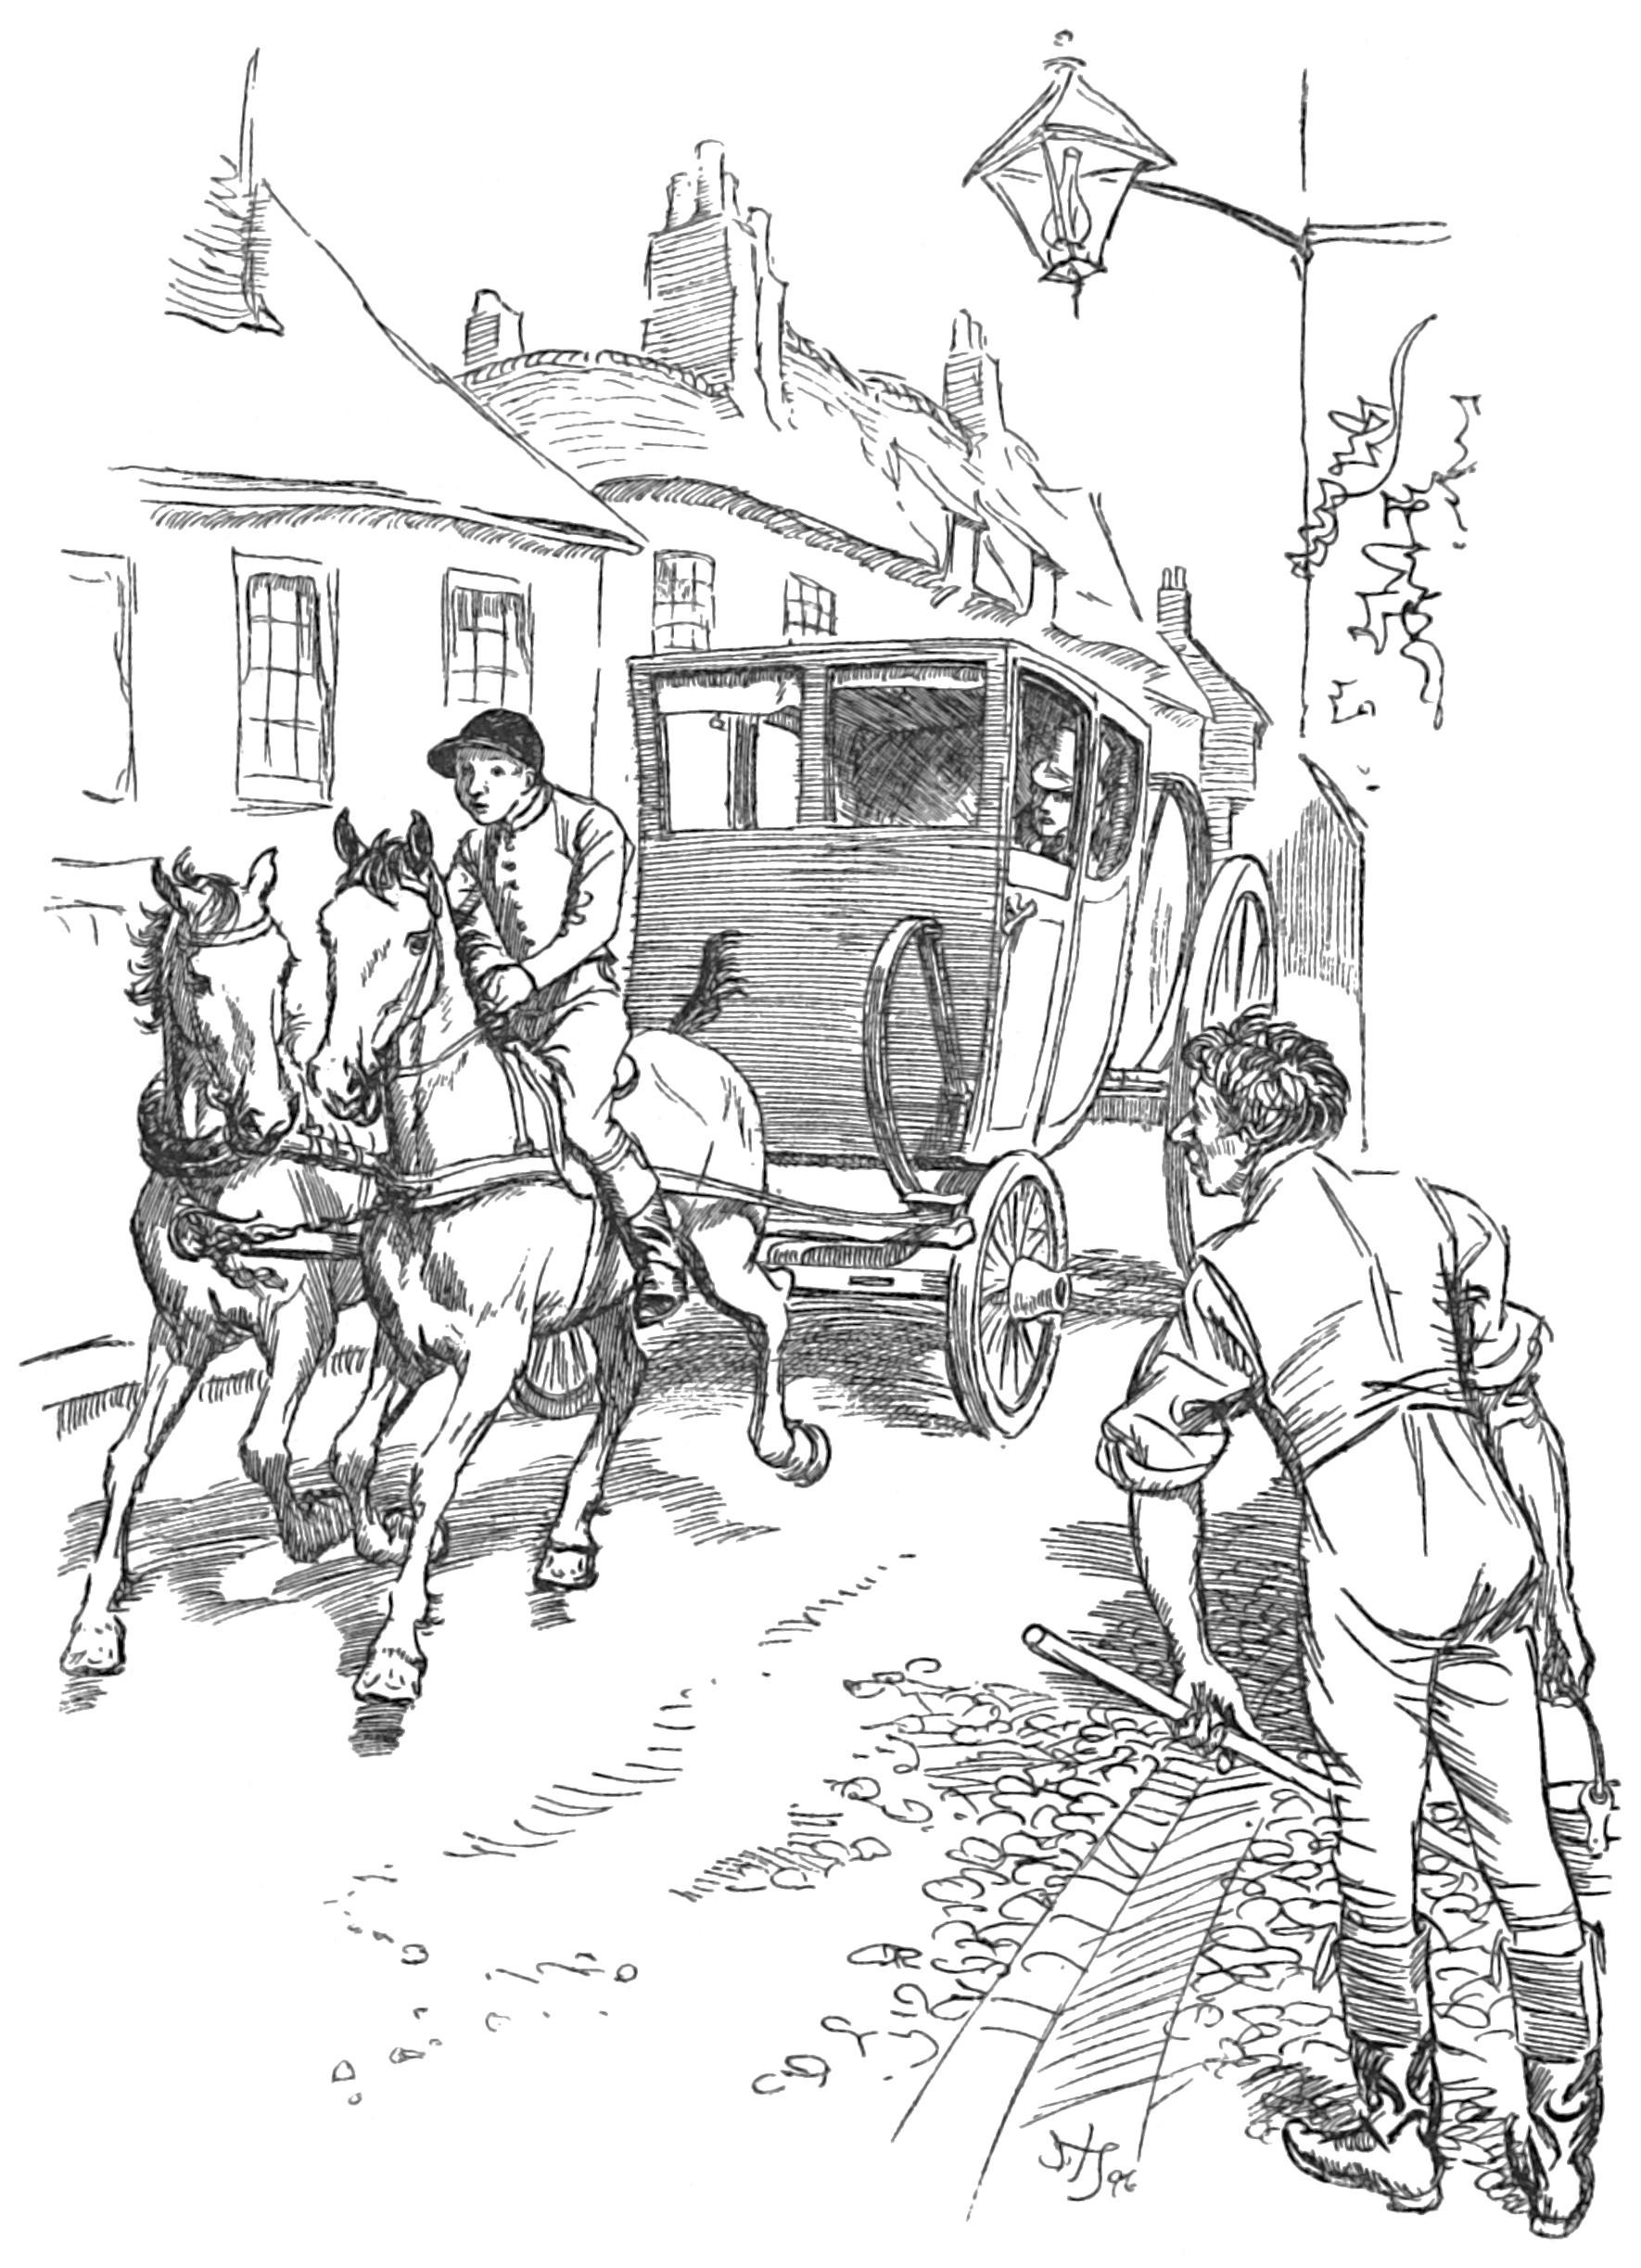
\includegraphics[width=\linewidth]{44chaise}
\caption{Seen the Crown chaise pass by}
\end{figure}

What Mr Elton had learned from the ostler on the subject, being the accumulation of the ostler's own knowledge, and the knowledge of the servants at Randalls, was, that a messenger had come over from Richmond soon after the return of the party from Box Hill—which messenger, however, had been no more than was expected; and that Mr Churchill had sent his nephew a few lines, containing, upon the whole, a tolerable account of Mrs Churchill, and only wishing him not to delay coming back beyond the next morning early; but that Mr Frank Churchill having resolved to go home directly, without waiting at all, and his horse seeming to have got a cold, Tom had been sent off immediately for the Crown chaise, and the ostler had stood out and seen it pass by, the boy going a good pace, and driving very steady.

There was nothing in all this either to astonish or interest, and it caught Emma's attention only as it united with the subject which already engaged her mind. The contrast between Mrs Churchill's importance in the world, and Jane Fairfax's, struck her; one was every thing, the other nothing—and she sat musing on the difference of woman's destiny, and quite unconscious on what her eyes were fixed, till roused by Miss Bates's saying,

»Aye, I see what you are thinking of, the pianoforte. What is to become of that?—Very true. Poor dear Jane was talking of it just now.—»You must go,« said she. »You and I must part. You will have no business here.—Let it stay, however,« said she; »give it houseroom till Colonel Campbell comes back. I shall talk about it to him; he will settle for me; he will help me out of all my difficulties.«—And to this day, I do believe, she knows not whether it was his present or his daughter's.«

Now Emma was obliged to think of the pianoforte; and the remembrance of all her former fanciful and unfair conjectures was so little pleasing, that she soon allowed herself to believe her visit had been long enough; and, with a repetition of every thing that she could venture to say of the good wishes which she really felt, took leave.
%!TeX root=../sensetop.tex
\chapter[Chapter \thechapter]{}
\lettrine[lraise=0.3]{E}{linor}, for some time after he left her, for some time even after the sound of his carriage had died away, remained too much oppressed by a crowd of ideas, widely differing in themselves, but of which sadness was the general result, to think even of her sister.

Willoughby, he, whom only half an hour ago she had abhorred as the most worthless of men, Willoughby, in spite of all his faults, excited a degree of commiseration for the sufferings produced by them, which made her think of him as now separated for ever from her family, with a tenderness, a regret, rather in proportion, as she soon acknowledged within herself—to his wishes than to his merits. She felt that his influence over her mind was heightened by circumstances which ought not in reason to have weight; by that person of uncommon attraction, that open, affectionate, and lively manner which it was no merit to possess; and by that still ardent love for Marianne, which it was not even innocent to indulge. But she felt that it was so, long, long before she could feel his influence less.

When at last she returned to the unconscious Marianne, she found her just awaking, refreshed by so long and sweet a sleep to the extent of her hopes. Elinor's heart was full. The past, the present, the future, Willoughby's visit, Marianne's safety, and her mother's expected arrival, threw her altogether into an agitation of spirits which kept off every indication of fatigue, and made her only fearful of betraying herself to her sister. Short was the time, however, in which that fear could affect her, for within half an hour after Willoughby's leaving the house, she was again called down stairs by the sound of another carriage.—Eager to save her mother from every unnecessary moment's horrible suspense, she ran immediately into the hall, and reached the outward door just in time to receive and support her as she entered it.

Mrs Dashwood, whose terror as they drew near the house had produced almost the conviction of Marianne's being no more, had no voice to inquire after her, no voice even for Elinor; but \textit{she}, waiting neither for salutation nor inquiry, instantly gave the joyful relief; and her mother, catching it with all her usual warmth, was in a moment as much overcome by her happiness, as she had been before by her fears. She was supported into the drawing-room between her daughter and her friend; and there, shedding tears of joy, though still unable to speak, embraced Elinor again and again, turning from her at intervals to press Colonel Brandon's hand, with a look which spoke at once her gratitude, and her conviction of his sharing with herself in the bliss of the moment. He shared it, however, in a silence even greater than her own.

As soon as Mrs Dashwood had recovered herself, to see Marianne was her first desire; and in two minutes she was with her beloved child, rendered dearer to her than ever by absence, unhappiness, and danger. Elinor's delight, as she saw what each felt in the meeting, was only checked by an apprehension of its robbing Marianne of farther sleep: but Mrs Dashwood could be calm, could be even prudent, when the life of a child was at stake, and Marianne, satisfied in knowing her mother was near her, and conscious of being too weak for conversation, submitted readily to the silence and quiet prescribed by every nurse around her. Mrs Dashwood \textit{would} sit up with her all night; and Elinor, in compliance with her mother's entreaty, went to bed. But the rest, which one night entirely sleepless, and many hours of the most wearing anxiety seemed to make requisite, was kept off by irritation of spirits. Willoughby, <poor Willoughby,> as she now allowed herself to call him, was constantly in her thoughts; she would not but have heard his vindication for the world, and now blamed, now acquitted herself for having judged him so harshly before. But her promise of relating it to her sister was invariably painful. She dreaded the performance of it, dreaded what its effect on Marianne might be; doubted whether after such an explanation she could ever be happy with another; and for a moment wished Willoughby a widower. Then, remembering Colonel Brandon, reproved herself, felt that to \textit{his} sufferings and \textit{his} constancy far more than to his rival's, the reward of her sister was due, and wished any thing rather than Mrs Willoughby's death.

The shock of Colonel Brandon's errand at Barton had been much softened to Mrs Dashwood by her own previous alarm; for so great was her uneasiness about Marianne, that she had already determined to set out for Cleveland on that very day, without waiting for any further intelligence, and had so far settled her journey before his arrival, that the Careys were then expected every moment to fetch Margaret away, as her mother was unwilling to take her where there might be infection.

Marianne continued to mend every day, and the brilliant cheerfulness of Mrs Dashwood's looks and spirits proved her to be, as she repeatedly declared herself, one of the happiest women in the world. Elinor could not hear the declaration, nor witness its proofs without sometimes wondering whether her mother ever recollected Edward. But Mrs Dashwood, trusting to the temperate account of her own disappointment which Elinor had sent her, was led away by the exuberance of her joy to think only of what would increase it. Marianne was restored to her from a danger in which, as she now began to feel, her own mistaken judgment in encouraging the unfortunate attachment to Willoughby, had contributed to place her;—and in her recovery she had yet another source of joy unthought of by Elinor. It was thus imparted to her, as soon as any opportunity of private conference between them occurred.

<At last we are alone. My Elinor, you do not yet know all my happiness. Colonel Brandon loves Marianne. He has told me so himself.>

Her daughter, feeling by turns both pleased and pained, surprised and not surprised, was all silent attention.

<You are never like me, dear Elinor, or I should wonder at your composure now. Had I sat down to wish for any possible good to my family, I should have fixed on Colonel Brandon's marrying one of you as the object most desirable. And I believe Marianne will be the most happy with him of the two.>

Elinor was half inclined to ask her reason for thinking so, because satisfied that none founded on an impartial consideration of their age, characters, or feelings, could be given;—but her mother must always be carried away by her imagination on any interesting subject, and therefore instead of an inquiry, she passed it off with a smile.

<He opened his whole heart to me yesterday as we travelled. It came out quite unawares, quite undesignedly. I, you may well believe, could talk of nothing but my child;—he could not conceal his distress; I saw that it equalled my own, and he perhaps, thinking that mere friendship, as the world now goes, would not justify so warm a sympathy—or rather, not thinking at all, I suppose—giving way to irresistible feelings, made me acquainted with his earnest, tender, constant, affection for Marianne. He has loved her, my Elinor, ever since the first moment of seeing her.>

Here, however, Elinor perceived,—not the language, not the professions of Colonel Brandon, but the natural embellishments of her mother's active fancy, which fashioned every thing delightful to her as it chose.

<His regard for her, infinitely surpassing anything that Willoughby ever felt or feigned, as much more warm, as more sincere or constant—which ever we are to call it—has subsisted through all the knowledge of dear Marianne's unhappy prepossession for that worthless young man!—and without selfishness—without encouraging a hope!—could he have seen her happy with another—Such a noble mind!—such openness, such sincerity!—no one can be deceived in \textit{him}.>

<Colonel Brandon's character,> said Elinor, <as an excellent man, is well established.>

<I know it is,>—replied her mother seriously, <or after such a warning, \textit{I} should be the last to encourage such affection, or even to be pleased by it. But his coming for me as he did, with such active, such ready friendship, is enough to prove him one of the worthiest of men.>

<His character, however,> answered Elinor, <does not rest on \textit{one} act of kindness, to which his affection for Marianne, were humanity out of the case, would have prompted him. To Mrs Jennings, to the Middletons, he has been long and intimately known; they equally love and respect him; and even my own knowledge of him, though lately acquired, is very considerable; and so highly do \textit{I} value and esteem him, that if Marianne can be happy with him, I shall be as ready as yourself to think our connection the greatest blessing to us in the world. What answer did you give him?—Did you allow him to hope?>

<Oh! my love, I could not then talk of hope to him or to myself. Marianne might at that moment be dying. But he did not ask for hope or encouragement. His was an involuntary confidence, an irrepressible effusion to a soothing friend, not an application to a parent. Yet after a time I \textit{did} say, for at first I was quite overcome, that if she lived, as I trusted she might, my greatest happiness would lie in promoting their marriage; and since our arrival, since our delightful security, I have repeated it to him more fully, have given him every encouragement in my power. Time, a very little time, I tell him, will do everything; Marianne's heart is not to be wasted for ever on such a man as Willoughby. His own merits must soon secure it.>

<To judge from the Colonel's spirits, however, you have not yet made him equally sanguine.>

<No. He thinks Marianne's affection too deeply rooted for any change in it under a great length of time, and even supposing her heart again free, is too diffident of himself to believe, that with such a difference of age and disposition he could ever attach her. There, however, he is quite mistaken. His age is only so much beyond hers as to be an advantage, as to make his character and principles fixed; and his disposition, I am well convinced, is exactly the very one to make your sister happy. And his person, his manners too, are all in his favour. My partiality does not blind me; he certainly is not so handsome as Willoughby; but at the same time, there is something much more pleasing in his countenance. There was always a something, if you remember, in Willoughby's eyes at times, which I did not like.>

Elinor could \textit{not} remember it; but her mother, without waiting for her assent, continued,

<And his manners, the Colonel's manners are not only more pleasing to me than Willoughby's ever were, but they are of a kind I well know to be more solidly attaching to Marianne. Their gentleness, their genuine attention to other people, and their manly unstudied simplicity is much more accordant with her real disposition, than the liveliness, often artificial, and often ill-timed of the other. I am very sure myself, that had Willoughby turned out as really amiable, as he has proved himself the contrary, Marianne would yet never have been so happy with \textit{him} as she will be with Colonel Brandon.>

She paused.—Her daughter could not quite agree with her, but her dissent was not heard, and therefore gave no offence.

<At Delaford, she will be within an easy distance of me,> added Mrs Dashwood, <even if I remain at Barton; and in all probability,—for I hear it is a large village,—indeed there certainly \textit{must} be some small house or cottage close by, that would suit us quite as well as our present situation.>

Poor Elinor!—here was a new scheme for getting her to Delaford!—but her spirit was stubborn.

<His fortune too!—for at my time of life you know, everybody cares about \textit{that};—and though I neither know nor desire to know, what it really is, I am sure it must be a good one.>

Here they were interrupted by the entrance of a third person, and Elinor withdrew to think it all over in private, to wish success to her friend, and yet in wishing it, to feel a pang for Willoughby.
%!TeX root=../sensetop.tex
\chapter[Chapter \thechapter]{}
\lettrine[lraise=0.3]{M}{arianne}'s illness, though weakening in its kind, had not been long enough to make her recovery slow; and with youth, natural strength, and her mother's presence in aid, it proceeded so smoothly as to enable her to remove, within four days after the arrival of the latter, into Mrs Palmer's dressing-room. When there, at her own particular request, for she was impatient to pour forth her thanks to him for fetching her mother, Colonel Brandon was invited to visit her.

His emotion on entering the room, in seeing her altered looks, and in receiving the pale hand which she immediately held out to him, was such, as, in Elinor's conjecture, must arise from something more than his affection for Marianne, or the consciousness of its being known to others; and she soon discovered in his melancholy eye and varying complexion as he looked at her sister, the probable recurrence of many past scenes of misery to his mind, brought back by that resemblance between Marianne and Eliza already acknowledged, and now strengthened by the hollow eye, the sickly skin, the posture of reclining weakness, and the warm acknowledgment of peculiar obligation.

Mrs Dashwood, not less watchful of what passed than her daughter, but with a mind very differently influenced, and therefore watching to very different effect, saw nothing in the Colonel's behaviour but what arose from the most simple and self-evident sensations, while in the actions and words of Marianne she persuaded herself to think that something more than gratitude already dawned.

At the end of another day or two, Marianne growing visibly stronger every twelve hours, Mrs Dashwood, urged equally by her own and her daughter's wishes, began to talk of removing to Barton. On \textit{her} measures depended those of her two friends; Mrs Jennings could not quit Cleveland during the Dashwoods' stay; and Colonel Brandon was soon brought, by their united request, to consider his own abode there as equally determinate, if not equally indispensable. At his and Mrs Jennings's united request in return, Mrs Dashwood was prevailed on to accept the use of his carriage on her journey back, for the better accommodation of her sick child; and the Colonel, at the joint invitation of Mrs Dashwood and Mrs Jennings, whose active good-nature made her friendly and hospitable for other people as well as herself, engaged with pleasure to redeem it by a visit at the cottage, in the course of a few weeks.

The day of separation and departure arrived; and Marianne, after taking so particular and lengthened a leave of Mrs Jennings, one so earnestly grateful, so full of respect and kind wishes as seemed due to her own heart from a secret acknowledgment of past inattention, and bidding Colonel Brandon farewell with a cordiality of a friend, was carefully assisted by him into the carriage, of which he seemed anxious that she should engross at least half. Mrs Dashwood and Elinor then followed, and the others were left by themselves, to talk of the travellers, and feel their own dullness, till Mrs Jennings was summoned to her chaise to take comfort in the gossip of her maid for the loss of her two young companions; and Colonel Brandon immediately afterwards took his solitary way to Delaford.

The Dashwoods were two days on the road, and Marianne bore her journey on both, without essential fatigue. Every thing that the most zealous affection, the most solicitous care could do to render her comfortable, was the office of each watchful companion, and each found their reward in her bodily ease, and her calmness of spirits. To Elinor, the observation of the latter was particularly grateful. She, who had seen her week after week so constantly suffering, oppressed by anguish of heart which she had neither courage to speak of, nor fortitude to conceal, now saw with a joy, which no other could equally share, an apparent composure of mind, which, in being the result as she trusted of serious reflection, must eventually lead her to contentment and cheerfulness.

As they approached Barton, indeed, and entered on scenes of which every field and every tree brought some peculiar, some painful recollection, she grew silent and thoughtful, and turning away her face from their notice, sat earnestly gazing through the window. But here, Elinor could neither wonder nor blame; and when she saw, as she assisted Marianne from the carriage, that she had been crying, she saw only an emotion too natural in itself to raise any thing less tender than pity, and in its unobtrusiveness entitled to praise. In the whole of her subsequent manner, she traced the direction of a mind awakened to reasonable exertion; for no sooner had they entered their common sitting-room, than Marianne turned her eyes around it with a look of resolute firmness, as if determined at once to accustom herself to the sight of every object with which the remembrance of Willoughby could be connected.—She said little, but every sentence aimed at cheerfulness, and though a sigh sometimes escaped her, it never passed away without the atonement of a smile. After dinner she would try her piano-forte. She went to it; but the music on which her eye first rested was an opera, procured for her by Willoughby, containing some of their favourite duets, and bearing on its outward leaf her own name in his hand-writing.—That would not do.—She shook her head, put the music aside, and after running over the keys for a minute, complained of feebleness in her fingers, and closed the instrument again; declaring however with firmness as she did so, that she should in future practice much.

The next morning produced no abatement in these happy symptoms. On the contrary, with a mind and body alike strengthened by rest, she looked and spoke with more genuine spirit, anticipating the pleasure of Margaret's return, and talking of the dear family party which would then be restored, of their mutual pursuits and cheerful society, as the only happiness worth a wish.

<When the weather is settled, and I have recovered my strength,> said she, <we will take long walks together every day. We will walk to the farm at the edge of the down, and see how the children go on; we will walk to Sir John's new plantations at Barton Cross, and the Abbeyland; and we will often go to the old ruins of the Priory, and try to trace its foundations as far as we are told they once reached. I know we shall be happy. I know the summer will pass happily away. I mean never to be later in rising than six, and from that time till dinner I shall divide every moment between music and reading. I have formed my plan, and am determined to enter on a course of serious study. Our own library is too well known to me, to be resorted to for any thing beyond mere amusement. But there are many works well worth reading at the Park; and there are others of more modern production which I know I can borrow of Colonel Brandon. By reading only six hours a-day, I shall gain in the course of a twelve-month a great deal of instruction which I now feel myself to want.>

\begin{figure}[tbph]
\centering
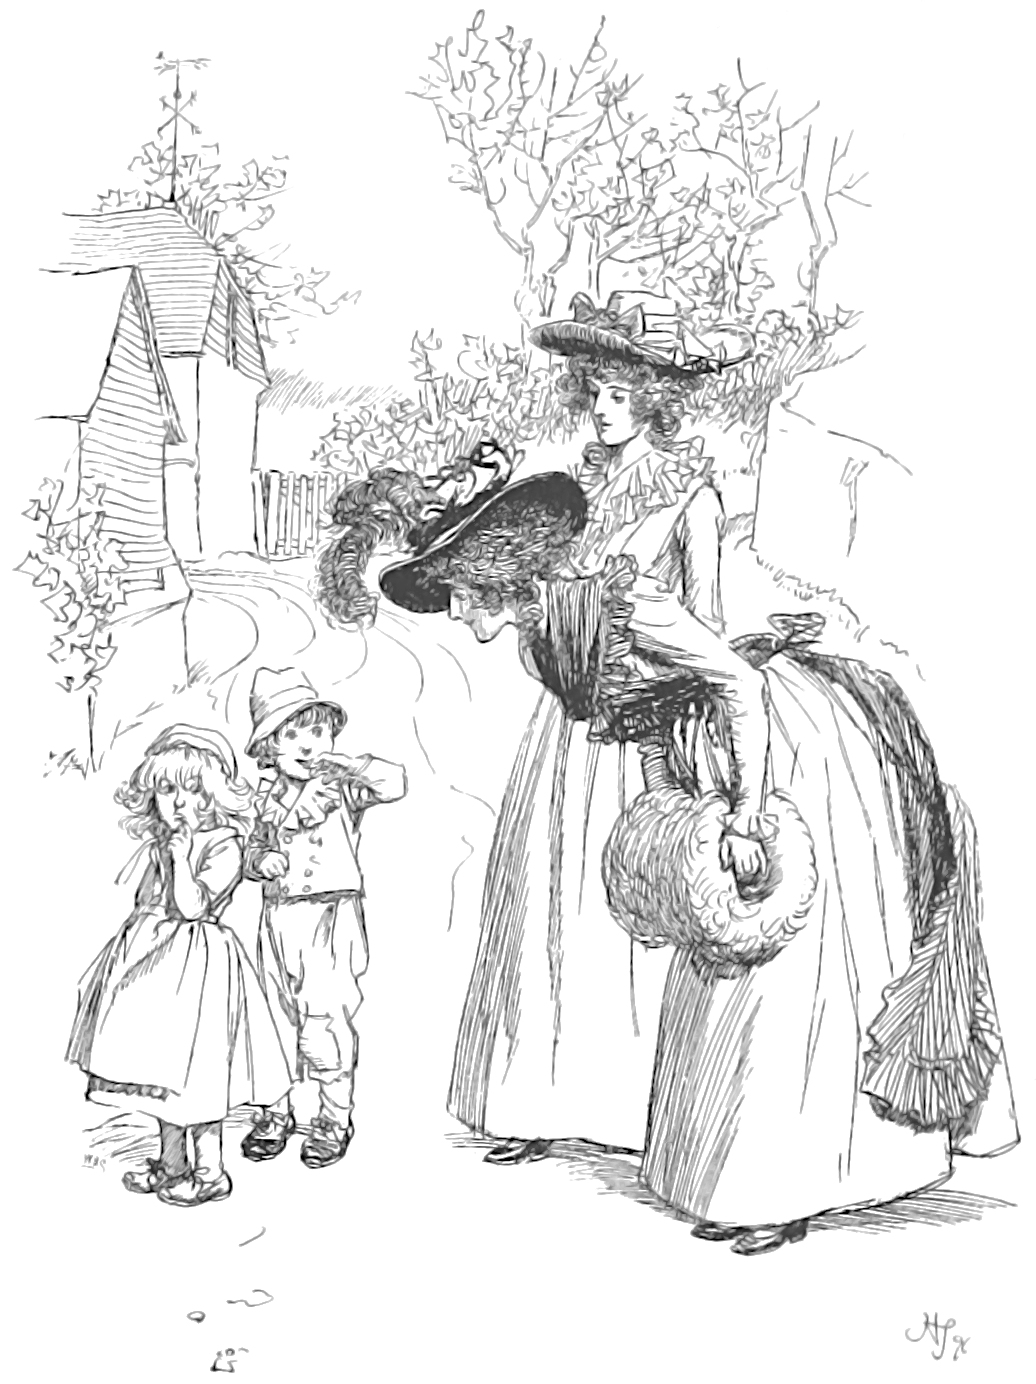
\includegraphics[width=\linewidth]{46children}
\caption{See how the children go on}
\end{figure}

Elinor honoured her for a plan which originated so nobly as this; though smiling to see the same eager fancy which had been leading her to the extreme of languid indolence and selfish repining, now at work in introducing excess into a scheme of such rational employment and virtuous self-control. Her smile however changed to a sigh when she remembered that promise to Willoughby was yet unfulfilled, and feared she had that to communicate which might again unsettle the mind of Marianne, and ruin at least for a time this fair prospect of busy tranquillity. Willing therefore to delay the evil hour, she resolved to wait till her sister's health were more secure, before she appointed it. But the resolution was made only to be broken.

Marianne had been two or three days at home, before the weather was fine enough for an invalid like herself to venture out. But at last a soft, genial morning appeared; such as might tempt the daughter's wishes and the mother's confidence; and Marianne, leaning on Elinor's arm, was authorised to walk as long as she could without fatigue, in the lane before the house.

The sisters set out at a pace, slow as the feebleness of Marianne in an exercise hitherto untried since her illness required; and they had advanced only so far beyond the house as to admit a full view of the hill, the important hill behind, when pausing with her eyes turned towards it, Marianne calmly said,—

<There, exactly there,>—pointing with one hand, <on that projecting mound,—there I fell; and there I first saw Willoughby.>

Her voice sunk with the word, but presently reviving she added,

<I am thankful to find that I can look with so little pain on the spot! shall we ever talk on that subject, Elinor?> hesitatingly it was said. <Or will it be wrong? I \textit{can} talk of it now, I hope, as I ought to do.>

Elinor tenderly invited her to be open.

<As for regret,> said Marianne, <I have done with that, as far as \textit{he} is concerned. I do not mean to talk to you of what my feelings have been for him, but what they are \textit{now}. At present, if I could be satisfied on one point, if I could be allowed to think that he was not \textit{always} acting a part, not \textit{always} deceiving me; but above all, if I could be assured that he never was so \textit{very} wicked as my fears have sometimes fancied him, since the story of that unfortunate girl\longdash>

She stopt. Elinor joyfully treasured her words as she answered,

<If you could be assured of that, you think you should be easy.>

<Yes. My peace of mind is doubly involved in it; for not only is it horrible to suspect a person, who has been what \textit{he} has been to \textit{me}, of such designs, but what must it make me appear to myself? What in a situation like mine, but a most shamefully unguarded affection could expose me to\longdash>

<How then,> asked her sister, <would you account for his behaviour?>

<I would suppose him,—Oh, how gladly would I suppose him, only fickle, very, very fickle.>

Elinor said no more. She was debating within herself on the eligibility of beginning her story directly, or postponing it till Marianne were in stronger health;—and they crept on for a few minutes in silence.

<I am not wishing him too much good,> said Marianne at last with a sigh, <when I wish his secret reflections may be no more unpleasant than my own. He will suffer enough in them.>

<Do you compare your conduct with his?>

<No. I compare it with what it ought to have been; I compare it with yours.>

<Our situations have borne little resemblance.>

<They have borne more than our conduct. Do not, my dearest Elinor, let your kindness defend what I know your judgment must censure. My illness has made me think. It has given me leisure and calmness for serious recollection. Long before I was enough recovered to talk, I was perfectly able to reflect. I considered the past: I saw in my own behaviour, since the beginning of our acquaintance with him last autumn, nothing but a series of imprudence towards myself, and want of kindness to others. I saw that my own feelings had prepared my sufferings, and that my want of fortitude under them had almost led me to the grave. My illness, I well knew, had been entirely brought on by myself by such negligence of my own health, as I had felt even at the time to be wrong. Had I died, it would have been self-destruction. I did not know my danger till the danger was removed; but with such feelings as these reflections gave me, I wonder at my recovery,—wonder that the very eagerness of my desire to live, to have time for atonement to my God, and to you all, did not kill me at once. Had I died, in what peculiar misery should I have left you, my nurse, my friend, my sister! You, who had seen all the fretful selfishness of my latter days; who had known all the murmurings of my heart! How should I have lived in \textit{your} remembrance! My mother too! How could you have consoled her! I cannot express my own abhorrence of myself. Whenever I looked towards the past, I saw some duty neglected, or some failing indulged. Every body seemed injured by me. The kindness, the unceasing kindness of Mrs Jennings, I had repaid with ungrateful contempt. To the Middletons, to the Palmers, the Steeles, to every common acquaintance even, I had been insolent and unjust; with a heart hardened against their merits, and a temper irritated by their very attention. To John, to Fanny, yes, even to them, little as they deserve, I had given less than their due. But you, you above all, above my mother, had been wronged by me. I, and only I, knew your heart and its sorrows; yet to what did it influence me?—not to any compassion that could benefit you or myself.—Your example was before me; but to what avail? Was I more considerate of you and your comfort? Did I imitate your forbearance, or lessen your restraints, by taking any part in those offices of general complaisance or particular gratitude which you had hitherto been left to discharge alone? No; not less when I knew you to be unhappy, than when I had believed you at ease, did I turn away from every exertion of duty or friendship; scarcely allowing sorrow to exist but with me, regretting only \textit{that} heart which had deserted and wronged me, and leaving you, for whom I professed an unbounded affection, to be miserable for my sake.>

Here ceased the rapid flow of her self-reproving spirit; and Elinor, impatient to soothe, though too honest to flatter, gave her instantly that praise and support which her frankness and her contrition so well deserved. Marianne pressed her hand and replied,—

<You are very good.—The future must be my proof. I have laid down my plan, and if I am capable of adhering to it—my feelings shall be governed and my temper improved. They shall no longer worry others, nor torture myself. I shall now live solely for my family. You, my mother, and Margaret, must henceforth be all the world to me; you will share my affections entirely between you. From you, from my home, I shall never again have the smallest incitement to move; and if I do mix in other society, it will be only to show that my spirit is humbled, my heart amended, and that I can practise the civilities, the lesser duties of life, with gentleness and forbearance. As for Willoughby—to say that I shall soon or that I shall ever forget him, would be idle. His remembrance can be overcome by no change of circumstances or opinions. But it shall be regulated, it shall be checked by religion, by reason, by constant employment.>

She paused—and added in a low voice, <If I could but know \textit{his} heart, everything would become easy.>

Elinor, who had now been for some time reflecting on the propriety or impropriety of speedily hazarding her narration, without feeling at all nearer decision than at first, heard this; and perceiving that as reflection did nothing, resolution must do all, soon found herself leading to the fact.

She managed the recital, as she hoped, with address; prepared her anxious listener with caution; related simply and honestly the chief points on which Willoughby grounded his apology; did justice to his repentance, and softened only his protestations of present regard. Marianne said not a word.—She trembled, her eyes were fixed on the ground, and her lips became whiter than even sickness had left them. A thousand inquiries sprung up from her heart, but she dared not urge one. She caught every syllable with panting eagerness; her hand, unknowingly to herself, closely pressed her sister's, and tears covered her cheeks.

Elinor, dreading her being tired, led her towards home; and till they reached the door of the cottage, easily conjecturing what her curiosity must be though no question was suffered to speak it, talked of nothing but Willoughby, and their conversation together; and was carefully minute in every particular of speech and look, where minuteness could be safely indulged. As soon as they entered the house, Marianne with a kiss of gratitude and these two words just articulate through her tears, <Tell mama,> withdrew from her sister and walked slowly up stairs. Elinor would not attempt to disturb a solitude so reasonable as what she now sought; and with a mind anxiously pre-arranging its result, and a resolution of reviving the subject again, should Marianne fail to do it, she turned into the parlour to fulfil her parting injunction.
%!TeX root=../pridetop.tex
\chapter[Chapter \thechapter]{}
	
	\begin{figure}[t!]
\centering
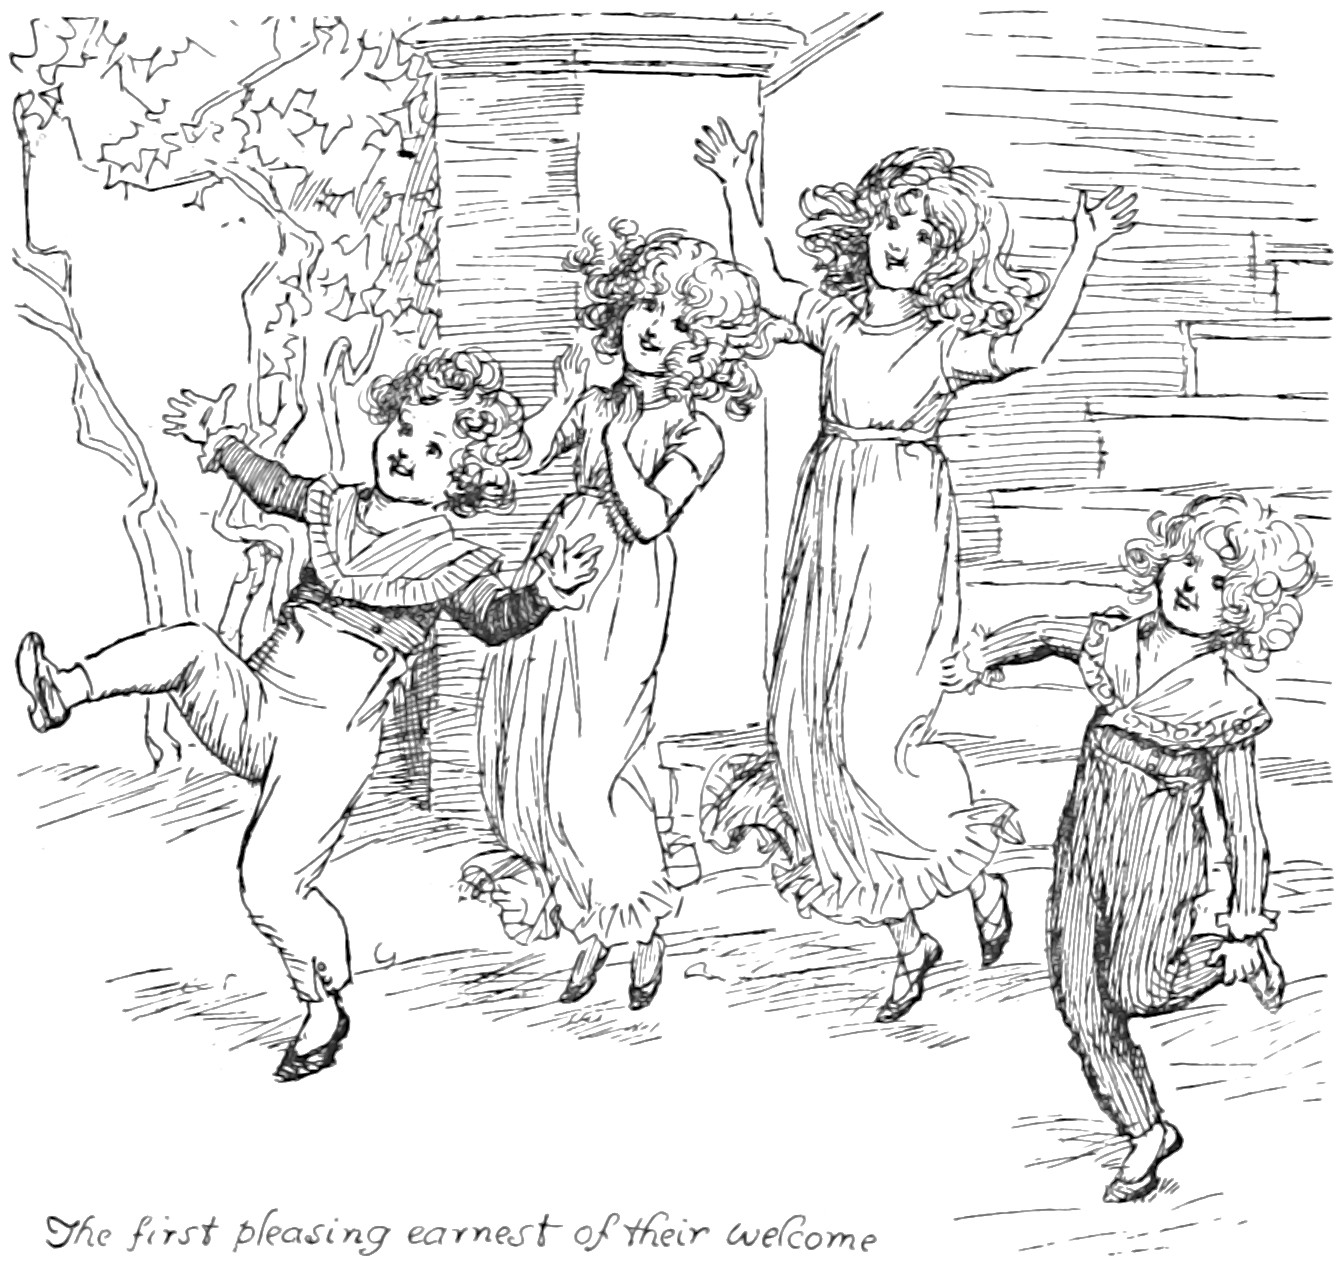
\includegraphics[width=.8\linewidth]{47top}
\captionlistentry{The first pleasing earnest of their welcome}
\end{figure}

\lettrine[lines=6,image=true,ante=`,loversize=.1,findent=2pt]{initials/chap47i}{} have been thinking it over again, Elizabeth,' said her uncle, as they drove from the town; »and really, upon serious consideration, I am much more inclined than I was to judge as your eldest sister does of the matter. It appears to me so very unlikely that any young man should form such a design against a girl who is by no means unprotected or friendless, and who was actually staying in his Colonel's family, that I am strongly inclined to hope the best. Could he expect that her friends would not step forward? Could he expect to be noticed again by the regiment, after such an affront to Colonel Forster? His temptation is not adequate to the risk.«

»Do you really think so?« cried Elizabeth, brightening up for a moment.

»Upon my word,« said Mrs Gardiner, »I begin to be of your uncle's opinion. It is really too great a violation of decency, honour, and interest, for him to be guilty of it. I cannot think so very ill of Wickham. Can you, yourself, Lizzie, so wholly give him up, as to believe him capable of it?«

»Not perhaps of neglecting his own interest. But of every other neglect I can believe him capable. If, indeed, it should be so! But I dare not hope it. Why should they not go on to Scotland, if that had been the case?«

»In the first place,« replied Mr Gardiner, »there is no absolute proof that they are not gone to Scotland.«

»Oh, but their removing from the chaise into a hackney coach is such a presumption! And, besides, no traces of them were to be found on the Barnet road.«

»Well, then,—supposing them to be in London—they may be there, though for the purpose of concealment, for no more exceptionable purpose. It is not likely that money should be very abundant on either side; and it might strike them that they could be more economically, though less expeditiously, married in London, than in Scotland.«

»But why all this secrecy? Why any fear of detection? Why must their marriage be private? Oh, no, no—this is not likely. His most particular friend, you see by Jane's account, was persuaded of his never intending to marry her. Wickham will never marry a woman without some money. He cannot afford it. And what claims has Lydia, what attractions has she beyond youth, health, and good humour, that could make him for her sake forego every chance of benefiting himself by marrying well? As to what restraint the apprehensions of disgrace in the corps might throw on a dishonourable elopement with her, I am not able to judge; for I know nothing of the effects that such a step might produce. But as to your other objection, I am afraid it will hardly hold good. Lydia has no brothers to step forward; and he might imagine, from my father's behaviour, from his indolence and the little attention he has ever seemed to give to what was going forward in his family, that \textit{he} would do as little and think as little about it, as any father could do, in such a matter.«

»But can you think that Lydia is so lost to everything but love of him, as to consent to live with him on any other terms than marriage?«

»It does seem, and it is most shocking, indeed,« replied Elizabeth, with tears in her eyes, »that a sister's sense of decency and virtue in such a point should admit of doubt. But, really, I know not what to say. Perhaps I am not doing her justice. But she is very young: she has never been taught to think on serious subjects; and for the last half year, nay, for a twelvemonth, she has been given up to nothing but amusement and vanity. She has been allowed to dispose of her time in the most idle and frivolous manner, and to adopt any opinions that came in her way. Since the ——shire were first quartered in Meryton, nothing but love, flirtation, and officers, have been in her head. She has been doing everything in her power, by thinking and talking on the subject, to give greater—what shall I call it?—susceptibility to her feelings; which are naturally lively enough. And we all know that Wickham has every charm of person and address that can captivate a woman.«

»But you see that Jane,« said her aunt, »does not think so ill of Wickham, as to believe him capable of the attempt.«

»Of whom does Jane ever think ill? And who is there, whatever might be their former conduct, that she would believe capable of such an attempt, till it were proved against them? But Jane knows, as well as I do, what Wickham really is. We both know that he has been profligate in every sense of the word; that he has neither integrity nor honour; that he is as false and deceitful as he is insinuating.«

»And do you really know all this?« cried Mrs Gardiner, whose curiosity as to the mode of her intelligence was all alive.

»I do, indeed,« replied Elizabeth, colouring. »I told you the other day of his infamous behaviour to Mr Darcy; and you, yourself, when last at Longbourn, heard in what manner he spoke of the man who had behaved with such forbearance and liberality towards him. And there are other circumstances which I am not at liberty—which it is not worth while to relate; but his lies about the whole Pemberley family are endless. From what he said of Miss Darcy, I was thoroughly prepared to see a proud, reserved, disagreeable girl. Yet he knew to the contrary himself. He must know that she was as amiable and unpretending as we have found her.«

»But does Lydia know nothing of this? can she be ignorant of what you and Jane seem so well to understand?«

»Oh, yes!—that, that is the worst of all. Till I was in Kent, and saw so much both of Mr Darcy and his relation Colonel Fitzwilliam, I was ignorant of the truth myself. And when I returned home the ——shire was to leave Meryton in a week or fortnight's time. As that was the case, neither Jane, to whom I related the whole, nor I, thought it necessary to make our knowledge public; for of what use could it apparently be to anyone, that the good opinion, which all the neighbourhood had of him, should then be overthrown? And even when it was settled that Lydia should go with Mrs Forster, the necessity of opening her eyes to his character never occurred to me. That \textit{she} could be in any danger from the deception never entered my head. That such a consequence as \textit{this} should ensue, you may easily believe was far enough from my thoughts.«

»When they all removed to Brighton, therefore, you had no reason, I suppose, to believe them fond of each other?«

»Not the slightest. I can remember no symptom of affection on either side; and had anything of the kind been perceptible, you must be aware that ours is not a family on which it could be thrown away. When first he entered the corps, she was ready enough to admire him; but so we all were. Every girl in or near Meryton was out of her senses about him for the first two months: but he never distinguished \textit{her} by any particular attention; and, consequently, after a moderate period of extravagant and wild admiration, her fancy for him gave way, and others of the regiment, who treated her with more distinction, again became her favourites.«

It may be easily believed, that however little of novelty could be added to their fears, hopes, and conjectures, on this interesting subject by its repeated discussion, no other could detain them from it long, during the whole of the journey. From Elizabeth's thoughts it was never absent. Fixed there by the keenest of all anguish, self-reproach, she could find no interval of ease or forgetfulness.

They travelled as expeditiously as possible; and sleeping one night on the road, reached Longbourn by dinnertime the next day. It was a comfort to Elizabeth to consider that Jane could not have been wearied by long expectations.

The little Gardiners, attracted by the sight of a chaise, were standing on the steps of the house, as they entered the paddock; and when the carriage drove up to the door, the joyful surprise that lighted up their faces and displayed itself over their whole bodies, in a variety of capers and frisks, was the first pleasing earnest of their welcome.

Elizabeth jumped out; and after giving each of them a hasty kiss, hurried into the vestibule, where Jane, who came running downstairs from her mother's apartment, immediately met her.

Elizabeth, as she affectionately embraced her, whilst tears filled the eyes of both, lost not a moment in asking whether anything had been heard of the fugitives.

»Not yet,« replied Jane. »But now that my dear uncle is come, I hope everything will be well.«

»Is my father in town?«

»Yes, he went on Tuesday, as I wrote you word.«

»And have you heard from him often?«

»We have heard only once. He wrote me a few lines on Wednesday, to say that he had arrived in safety, and to give me his directions, which I particularly begged him to do. He merely added, that he should not write again, till he had something of importance to mention.«

»And my mother—how is she? How are you all?«

»My mother is tolerably well, I trust; though her spirits are greatly shaken. She is upstairs, and will have great satisfaction in seeing you all. She does not yet leave her dressing-room. Mary and Kitty, thank Heaven! are quite well.«

»But you—how are you?« cried Elizabeth. »You look pale. How much you must have gone through!«

Her sister, however, assured her of her being perfectly well; and their conversation, which had been passing while Mr and Mrs Gardiner were engaged with their children, was now put an end to by the approach of the whole party. Jane ran to her uncle and aunt, and welcomed and thanked them both, with alternate smiles and tears.

When they were all in the drawing-room, the questions which Elizabeth had already asked were of course repeated by the others, and they soon found that Jane had no intelligence to give. The sanguine hope of good, however, which the benevolence of her heart suggested, had not yet deserted her; she still expected that it would all end well, and that every morning would bring some letter, either from Lydia or her father, to explain their proceedings, and, perhaps, announce the marriage.

Mrs Bennet, to whose apartment they all repaired, after a few minutes' conversation together, received them exactly as might be expected; with tears and lamentations of regret, invectives against the villainous conduct of Wickham, and complaints of her own sufferings and ill-usage; blaming everybody but the person to whose ill-judging indulgence the errors of her daughter must be principally owing.

»If I had been able,« said she, »to carry my point in going to Brighton with all my family, \textit{this} would not have happened: but poor dear Lydia had nobody to take care of her. Why did the Forsters ever let her go out of their sight? I am sure there was some great neglect or other on their side, for she is not the kind of girl to do such a thing, if she had been well looked after. I always thought they were very unfit to have the charge of her; but I was over-ruled, as I always am. Poor, dear child! And now here's Mr Bennet gone away, and I know he will fight Wickham, wherever he meets him, and then he will be killed, and what is to become of us all? The Collinses will turn us out, before he is cold in his grave; and if you are not kind to us, brother, I do not know what we shall do.«

They all exclaimed against such terrific ideas; and Mr Gardiner, after general assurances of his affection for her and all her family, told her that he meant to be in London the very next day, and would assist Mr Bennet in every endeavour for recovering Lydia.

»Do not give way to useless alarm,« added he: »though it is right to be prepared for the worst, there is no occasion to look on it as certain. It is not quite a week since they left Brighton. In a few days more, we may gain some news of them; and till we know that they are not married, and have no design of marrying, do not let us give the matter over as lost. As soon as I get to town, I shall go to my brother, and make him come home with me to Gracechurch Street, and then we may consult together as to what is to be done.«

»Oh, my dear brother,« replied Mrs Bennet, »that is exactly what I could most wish for. And now do, when you get to town, find them out, wherever they may be; and if they are not married already, \textit{make} them marry. And as for wedding clothes, do not let them wait for that, but tell Lydia she shall have as much money as she chooses to buy them, after they are married. And, above all things, keep Mr Bennet from fighting. Tell him what a dreadful state I am in—that I am frightened out of my wits; and have such tremblings, such flutterings all over me, such spasms in my side, and pains in my head, and such beatings at my heart, that I can get no rest by night nor by day. And tell my dear Lydia not to give any directions about her clothes till she has seen me, for she does not know which are the best warehouses. Oh, brother, how kind you are! I know you will contrive it all.«

But Mr Gardiner, though he assured her again of his earnest endeavours in the cause, could not avoid recommending moderation to her, as well in her hopes as her fears; and after talking with her in this manner till dinner was on table, they left her to vent all her feelings on the housekeeper, who attended in the absence of her daughters.

Though her brother and sister were persuaded that there was no real occasion for such a seclusion from the family, they did not attempt to oppose it; for they knew that she had not prudence enough to hold her tongue before the servants, while they waited at table, and judged it better that \textit{one} only of the household, and the one whom they could most trust, should comprehend all her fears and solicitude on the subject.

In the dining-room they were soon joined by Mary and Kitty, who had been too busily engaged in their separate apartments to make their appearance before. One came from her books, and the other from her toilette. The faces of both, however, were tolerably calm; and no change was visible in either, except that the loss of her favourite sister, or the anger which she had herself incurred in the business, had given something more of fretfulness than usual to the accents of Kitty. As for Mary, she was mistress enough of herself to whisper to Elizabeth, with a countenance of grave reflection, soon after they were seated at table,—

»This is a most unfortunate affair, and will probably be much talked of. But we must stem the tide of malice, and pour into the wounded bosoms of each other the balm of sisterly consolation.«

Then perceiving in Elizabeth no inclination of replying, she added, »Unhappy as the event must be for Lydia, we may draw from it this useful lesson:—that loss of virtue in a female is irretrievable, that one false step involves her in endless ruin, that her reputation is no less brittle than it is beautiful, and that she cannot be too much guarded in her behaviour towards the undeserving of the other sex.«

Elizabeth lifted up her eyes in amazement, but was too much oppressed to make any reply. Mary, however, continued to console herself with such kind of moral extractions from the evil before them.

In the afternoon, the two elder Miss Bennets were able to be for half an hour by themselves; and Elizabeth instantly availed herself of the opportunity of making any inquiries which Jane was equally eager to satisfy. After joining in general lamentations over the dreadful sequel of this event, which Elizabeth considered as all but certain, and Miss Bennet could not assert to be wholly impossible, the former continued the subject by saying, »But tell me all and everything about it which I have not already heard. Give me further particulars. What did Colonel Forster say? Had they no apprehension of anything before the elopement took place? They must have seen them together for ever.«

»Colonel Forster did own that he had often suspected some partiality, especially on Lydia's side, but nothing to give him any alarm. I am so grieved for him. His behaviour was attentive and kind to the utmost. He \textit{was} coming to us, in order to assure us of his concern, before he had any idea of their not being gone to Scotland: when that apprehension first got abroad, it hastened his journey.«

»And was Denny convinced that Wickham would not marry? Did he know of their intending to go off? Had Colonel Forster seen Denny himself?«

»Yes; but when questioned by \textit{him}, Denny denied knowing anything of their plan, and would not give his real opinion about it. He did not repeat his persuasion of their not marrying, and from \textit{that} I am inclined to hope he might have been misunderstood before.«

»And till Colonel Forster came himself, not one of you entertained a doubt, I suppose, of their being really married?«

»How was it possible that such an idea should enter our brains? I felt a little uneasy—a little fearful of my sister's happiness with him in marriage, because I knew that his conduct had not been always quite right. My father and mother knew nothing of that; they only felt how imprudent a match it must be. Kitty then owned, with a very natural triumph on knowing more than the rest of us, that in Lydia's last letter she had prepared her for such a step. She had known, it seems, of their being in love with each other many weeks.«

»But not before they went to Brighton?«

»No, I believe not.«

»And did Colonel Forster appear to think ill of Wickham himself? Does he know his real character?«

»I must confess that he did not speak so well of Wickham as he formerly did. He believed him to be imprudent and extravagant; and since this sad affair has taken place, it is said that he left Meryton greatly in debt: but I hope this may be false.«

»Oh, Jane, had we been less secret, had we told what we knew of him, this could not have happened!«

»Perhaps it would have been better,« replied her sister.

»But to expose the former faults of any person, without knowing what their present feelings were, seemed unjustifiable.«

»We acted with the best intentions.«

»Could Colonel Forster repeat the particulars of Lydia's note to his wife?«

»He brought it with him for us to see.«

Jane then took it from her pocket-book, and gave it to Elizabeth. These were the contents:—


\begin{quotation}
\noindent My dear Harriet,\\

\indent You will laugh when you know where I am gone, and I cannot help laughing myself at your surprise to-morrow morning, as soon as I am missed. I am going to Gretna Green, and if you cannot guess with who, I shall think you a simpleton, for there is but one man in the world I love, and he is an angel. I should never be happy without him, so think it no harm to be off. You need not send them word at Longbourn of my going, if you do not like it, for it will make the surprise the greater when I write to them, and sign my name Lydia Wickham. What a good joke it will be! I can hardly write for laughing. Pray make my excuses to Pratt for not keeping my engagement, and dancing with him to-night. Tell him I hope he will excuse me when he knows all, and tell him I will dance with him at the next ball we meet with great pleasure. I shall send for my clothes when I get to Longbourn; but I wish you would tell Sally to mend a great slit in my worked muslin gown before they are packed up. Good-bye. Give my love to Colonel Forster. I hope you will drink to our good journey.

\begin{flushright}
Your affectionate friend,\\
\textsc{Lydia Bennet.}
\end{flushright}
\end{quotation}


»Oh, thoughtless, thoughtless Lydia!« cried Elizabeth when she had finished it. »What a letter is this, to be written at such a moment! But at least it shows that \textit{she} was serious in the object of her journey. Whatever he might afterwards persuade her to, it was not on her side a \textit{scheme} of infamy. My poor father! how he must have felt it!«

»I never saw anyone so shocked. He could not speak a word for full ten minutes. My mother was taken ill immediately, and the whole house in such confusion!«

»Oh, Jane,« cried Elizabeth, »was there a servant belonging to it who did not know the whole story before the end of the day?«

»I do not know: I hope there was. But to be guarded at such a time is very difficult. My mother was in hysterics; and though I endeavoured to give her every assistance in my power, I am afraid I did not do so much as I might have done. But the horror of what might possibly happen almost took from me my faculties.«

»Your attendance upon her has been too much for you. You do not look well. Oh that I had been with you! you have had every care and anxiety upon yourself alone.«

»Mary and Kitty have been very kind, and would have shared in every fatigue, I am sure, but I did not think it right for either of them. Kitty is slight and delicate, and Mary studies so much that her hours of repose should not be broken in on. My aunt Philips came to Longbourn on Tuesday, after my father went away; and was so good as to stay till Thursday with me. She was of great use and comfort to us all, and Lady Lucas has been very kind: she walked here on Wednesday morning to condole with us, and offered her services, or any of her daughters, if they could be of use to us.«

»She had better have stayed at home,« cried Elizabeth: »perhaps she \textit{meant} well, but, under such a misfortune as this, one cannot see too little of one's neighbours. Assistance is impossible; condolence, insufferable. Let them triumph over us at a distance, and be satisfied.«

She then proceeded to inquire into the measures which her father had intended to pursue, while in town, for the recovery of his daughter.

»He meant, I believe,« replied Jane, »to go to Epsom, the place where they last changed horses, see the postilions, and try if anything could be made out from them. His principal object must be to discover the number of the hackney coach which took them from Clapham. It had come with a fare from London; and as he thought the circumstance of a gentleman and lady's removing from one carriage into another might be remarked, he meant to make inquiries at Clapham. If he could anyhow discover at what house the coachman had before set down his fare, he determined to make inquiries there, and hoped it might not be impossible to find out the stand and number of the coach. I do not know of any other designs that he had formed; but he was in such a hurry to be gone, and his spirits so greatly discomposed, that I had difficulty in finding out even so much as this.«
\chapter[Chapter \thechapter]{} 

 \lettrine[lraise=0.3]{L}{et} other pens dwell on guilt and misery. I quit such odious subjects as soon as I can, impatient to restore everybody, not greatly in fault themselves, to tolerable comfort, and to have done with all the rest.

My Fanny, indeed, at this very time, I have the satisfaction of knowing, must have been happy in spite of everything. She must have been a happy creature in spite of all that she felt, or thought she felt, for the distress of those around her. She had sources of delight that must force their way. She was returned to Mansfield Park, she was useful, she was beloved; she was safe from Mr~Crawford; and when Sir~Thomas came back she had every proof that could be given in his then melancholy state of spirits, of his perfect approbation and increased regard; and happy as all this must make her, she would still have been happy without any of it, for Edmund was no longer the dupe of Miss~Crawford.

It is true that Edmund was very far from happy himself. He was suffering from disappointment and regret, grieving over what was, and wishing for what could never be. She knew it was so, and was sorry; but it was with a sorrow so founded on satisfaction, so tending to ease, and so much in harmony with every dearest sensation, that there are few who might not have been glad to exchange their greatest gaiety for it.

Sir~Thomas, poor Sir~Thomas, a parent, and conscious of errors in his own conduct as a parent, was the longest to suffer. He felt that he ought not to have allowed the marriage; that his daughter's sentiments had been sufficiently known to him to render him culpable in authorising it; that in so doing he had sacrificed the right to the expedient, and been governed by motives of selfishness and worldly wisdom. These were reflections that required some time to soften; but time will do almost everything; and though little comfort arose on Mrs~Rushworth's side for the misery she had occasioned, comfort was to be found greater than he had supposed in his other children. Julia's match became a less desperate business than he had considered it at first. She was humble, and wishing to be forgiven; and Mr~Yates, desirous of being really received into the family, was disposed to look up to him and be guided. He was not very solid; but there was a hope of his becoming less trifling, of his being at least tolerably domestic and quiet; and at any rate, there was comfort in finding his estate rather more, and his debts much less, than he had feared, and in being consulted and treated as the friend best worth attending to. There was comfort also in Tom, who gradually regained his health, without regaining the thoughtlessness and selfishness of his previous habits. He was the better for ever for his illness. He had suffered, and he had learned to think: two advantages that he had never known before; and the self-reproach arising from the deplorable event in Wimpole Street, to which he felt himself accessory by all the dangerous intimacy of his unjustifiable theatre, made an impression on his mind which, at the age of six-and-twenty, with no want of sense or good companions, was durable in its happy effects. He became what he ought to be: useful to his father, steady and quiet, and not living merely for himself.

Here was comfort indeed! and quite as soon as Sir~Thomas could place dependence on such sources of good, Edmund was contributing to his father's ease by improvement in the only point in which he had given him pain before—improvement in his spirits. After wandering about and sitting under trees with Fanny all the summer evenings, he had so well talked his mind into submission as to be very tolerably cheerful again.

These were the circumstances and the hopes which gradually brought their alleviation to Sir~Thomas, deadening his sense of what was lost, and in part reconciling him to himself; though the anguish arising from the conviction of his own errors in the education of his daughters was never to be entirely done away.

Too late he became aware how unfavourable to the character of any young people must be the totally opposite treatment which Maria and Julia had been always experiencing at home, where the excessive indulgence and flattery of their aunt had been continually contrasted with his own severity. He saw how ill he had judged, in expecting to counteract what was wrong in Mrs~Norris by its reverse in himself; clearly saw that he had but increased the evil by teaching them to repress their spirits in his presence so as to make their real disposition unknown to him, and sending them for all their indulgences to a person who had been able to attach them only by the blindness of her affection, and the excess of her praise.

Here had been grievous mismanagement; but, bad as it was, he gradually grew to feel that it had not been the most direful mistake in his plan of education. Something must have been wanting \textit{within}, or time would have worn away much of its ill effect. He feared that principle, active principle, had been wanting; that they had never been properly taught to govern their inclinations and tempers by that sense of duty which can alone suffice. They had been instructed theoretically in their religion, but never required to bring it into daily practice. To be distinguished for elegance and accomplishments, the authorised object of their youth, could have had no useful influence that way, no moral effect on the mind. He had meant them to be good, but his cares had been directed to the understanding and manners, not the disposition; and of the necessity of self-denial and humility, he feared they had never heard from any lips that could profit them.

Bitterly did he deplore a deficiency which now he could scarcely comprehend to have been possible. Wretchedly did he feel, that with all the cost and care of an anxious and expensive education, he had brought up his daughters without their understanding their first duties, or his being acquainted with their character and temper.

The high spirit and strong passions of Mrs~Rushworth, especially, were made known to him only in their sad result. She was not to be prevailed on to leave Mr~Crawford. She hoped to marry him, and they continued together till she was obliged to be convinced that such hope was vain, and till the disappointment and wretchedness arising from the conviction rendered her temper so bad, and her feelings for him so like hatred, as to make them for a while each other's punishment, and then induce a voluntary separation.

She had lived with him to be reproached as the ruin of all his happiness in Fanny, and carried away no better consolation in leaving him than that she \textit{had}  divided them. What can exceed the misery of such a mind in such a situation?

Mr~Rushworth had no difficulty in procuring a divorce; and so ended a marriage contracted under such circumstances as to make any better end the effect of good luck not to be reckoned on. She had despised him, and loved another; and he had been very much aware that it was so. The indignities of stupidity, and the disappointments of selfish passion, can excite little pity. His punishment followed his conduct, as did a deeper punishment the deeper guilt of his wife. \textit{He}  was released from the engagement to be mortified and unhappy, till some other pretty girl could attract him into matrimony again, and he might set forward on a second, and, it is to be hoped, more prosperous trial of the state: if duped, to be duped at least with good humour and good luck; while she must withdraw with infinitely stronger feelings to a retirement and reproach which could allow no second spring of hope or character.

Where she could be placed became a subject of most melancholy and momentous consultation. Mrs~Norris, whose attachment seemed to augment with the demerits of her niece, would have had her received at home and countenanced by them all. Sir~Thomas would not hear of it; and Mrs~Norris's anger against Fanny was so much the greater, from considering \textit{her}  residence there as the motive. She persisted in placing his scruples to \textit{her}  account, though Sir~Thomas very solemnly assured her that, had there been no young woman in question, had there been no young person of either sex belonging to him, to be endangered by the society or hurt by the character of Mrs~Rushworth, he would never have offered so great an insult to the neighbourhood as to expect it to notice her. As a daughter, he hoped a penitent one, she should be protected by him, and secured in every comfort, and supported by every encouragement to do right, which their relative situations admitted; but farther than \textit{that}  he could not go. Maria had destroyed her own character, and he would not, by a vain attempt to restore what never could be restored, by affording his sanction to vice, or in seeking to lessen its disgrace, be anywise accessory to introducing such misery in another man's family as he had known himself.

It ended in Mrs~Norris's resolving to quit Mansfield and devote herself to her unfortunate Maria, and in an establishment being formed for them in another country, remote and private, where, shut up together with little society, on one side no affection, on the other no judgment, it may be reasonably supposed that their tempers became their mutual punishment.

Mrs~Norris's removal from Mansfield was the great supplementary comfort of Sir~Thomas's life. His opinion of her had been sinking from the day of his return from Antigua: in every transaction together from that period, in their daily intercourse, in business, or in chat, she had been regularly losing ground in his esteem, and convincing him that either time had done her much disservice, or that he had considerably over-rated her sense, and wonderfully borne with her manners before. He had felt her as an hourly evil, which was so much the worse, as there seemed no chance of its ceasing but with life; she seemed a part of himself that must be borne for ever. To be relieved from her, therefore, was so great a felicity that, had she not left bitter remembrances behind her, there might have been danger of his learning almost to approve the evil which produced such a good.

She was regretted by no one at Mansfield. She had never been able to attach even those she loved best; and since Mrs~Rushworth's elopement, her temper had been in a state of such irritation as to make her everywhere tormenting. Not even Fanny had tears for aunt Norris, not even when she was gone for ever.

That Julia escaped better than Maria was owing, in some measure, to a favourable difference of disposition and circumstance, but in a greater to her having been less the darling of that very aunt, less flattered and less spoilt. Her beauty and acquirements had held but a second place. She had been always used to think herself a little inferior to Maria. Her temper was naturally the easiest of the two; her feelings, though quick, were more controllable, and education had not given her so very hurtful a degree of self-consequence.

She had submitted the best to the disappointment in Henry Crawford. After the first bitterness of the conviction of being slighted was over, she had been tolerably soon in a fair way of not thinking of him again; and when the acquaintance was renewed in town, and Mr~Rushworth's house became Crawford's object, she had had the merit of withdrawing herself from it, and of chusing that time to pay a visit to her other friends, in order to secure herself from being again too much attracted. This had been her motive in going to her cousin's. Mr~Yates's convenience had had nothing to do with it. She had been allowing his attentions some time, but with very little idea of ever accepting him; and had not her sister's conduct burst forth as it did, and her increased dread of her father and of home, on that event, imagining its certain consequence to herself would be greater severity and restraint, made her hastily resolve on avoiding such immediate horrors at all risks, it is probable that Mr~Yates would never have succeeded. She had not eloped with any worse feelings than those of selfish alarm. It had appeared to her the only thing to be done. Maria's guilt had induced Julia's folly.

Henry Crawford, ruined by early independence and bad domestic example, indulged in the freaks of a cold-blooded vanity a little too long. Once it had, by an opening undesigned and unmerited, led him into the way of happiness. Could he have been satisfied with the conquest of one amiable woman's affections, could he have found sufficient exultation in overcoming the reluctance, in working himself into the esteem and tenderness of Fanny Price, there would have been every probability of success and felicity for him. His affection had already done something. Her influence over him had already given him some influence over her. Would he have deserved more, there can be no doubt that more would have been obtained, especially when that marriage had taken place, which would have given him the assistance of her conscience in subduing her first inclination, and brought them very often together. Would he have persevered, and uprightly, Fanny must have been his reward, and a reward very voluntarily bestowed, within a reasonable period from Edmund's marrying Mary.

Had he done as he intended, and as he knew he ought, by going down to Everingham after his return from Portsmouth, he might have been deciding his own happy destiny. But he was pressed to stay for Mrs~Fraser's party; his staying was made of flattering consequence, and he was to meet Mrs~Rushworth there. Curiosity and vanity were both engaged, and the temptation of immediate pleasure was too strong for a mind unused to make any sacrifice to right: he resolved to defer his Norfolk journey, resolved that writing should answer the purpose of it, or that its purpose was unimportant, and staid. He saw Mrs~Rushworth, was received by her with a coldness which ought to have been repulsive, and have established apparent indifference between them for ever; but he was mortified, he could not bear to be thrown off by the woman whose smiles had been so wholly at his command: he must exert himself to subdue so proud a display of resentment; it was anger on Fanny's account; he must get the better of it, and make Mrs~Rushworth Maria Bertram again in her treatment of himself.

In this spirit he began the attack, and by animated perseverance had soon re-established the sort of familiar intercourse, of gallantry, of flirtation, which bounded his views; but in triumphing over the discretion which, though beginning in anger, might have saved them both, he had put himself in the power of feelings on her side more strong than he had supposed. She loved him; there was no withdrawing attentions avowedly dear to her. He was entangled by his own vanity, with as little excuse of love as possible, and without the smallest inconstancy of mind towards her cousin. To keep Fanny and the Bertrams from a knowledge of what was passing became his first object. Secrecy could not have been more desirable for Mrs~Rushworth's credit than he felt it for his own. When he returned from Richmond, he would have been glad to see Mrs~Rushworth no more. All that followed was the result of her imprudence; and he went off with her at last, because he could not help it, regretting Fanny even at the moment, but regretting her infinitely more when all the bustle of the intrigue was over, and a very few months had taught him, by the force of contrast, to place a yet higher value on the sweetness of her temper, the purity of her mind, and the excellence of her principles.

That punishment, the public punishment of disgrace, should in a just measure attend \textit{his}  share of the offence is, we know, not one of the barriers which society gives to virtue. In this world the penalty is less equal than could be wished; but without presuming to look forward to a juster appointment hereafter, we may fairly consider a man of sense, like Henry Crawford, to be providing for himself no small portion of vexation and regret: vexation that must rise sometimes to self-reproach, and regret to wretchedness, in having so requited hospitality, so injured family peace, so forfeited his best, most estimable, and endeared acquaintance, and so lost the woman whom he had rationally as well as passionately loved.

After what had passed to wound and alienate the two families, the continuance of the Bertrams and Grants in such close neighbourhood would have been most distressing; but the absence of the latter, for some months purposely lengthened, ended very fortunately in the necessity, or at least the practicability, of a permanent removal. Dr~Grant, through an interest on which he had almost ceased to form hopes, succeeded to a stall in Westminster, which, as affording an occasion for leaving Mansfield, an excuse for residence in London, and an increase of income to answer the expenses of the change, was highly acceptable to those who went and those who staid.

Mrs~Grant, with a temper to love and be loved, must have gone with some regret from the scenes and people she had been used to; but the same happiness of disposition must in any place, and any society, secure her a great deal to enjoy, and she had again a home to offer Mary; and Mary had had enough of her own friends, enough of vanity, ambition, love, and disappointment in the course of the last half-year, to be in need of the true kindness of her sister's heart, and the rational tranquillity of her ways. They lived together; and when Dr~Grant had brought on apoplexy and death, by three great institutionary dinners in one week, they still lived together; for Mary, though perfectly resolved against ever attaching herself to a younger brother again, was long in finding among the dashing representatives, or idle heir-apparents, who were at the command of her beauty, and her \textsterling 20,000, any one who could satisfy the better taste she had acquired at Mansfield, whose character and manners could authorise a hope of the domestic happiness she had there learned to estimate, or put Edmund Bertram sufficiently out of her head.

Edmund had greatly the advantage of her in this respect. He had not to wait and wish with vacant affections for an object worthy to succeed her in them. Scarcely had he done regretting Mary Crawford, and observing to Fanny how impossible it was that he should ever meet with such another woman, before it began to strike him whether a very different kind of woman might not do just as well, or a great deal better: whether Fanny herself were not growing as dear, as important to him in all her smiles and all her ways, as Mary Crawford had ever been; and whether it might not be a possible, a hopeful undertaking to persuade her that her warm and sisterly regard for him would be foundation enough for wedded love.

I purposely abstain from dates on this occasion, that every one may be at liberty to fix their own, aware that the cure of unconquerable passions, and the transfer of unchanging attachments, must vary much as to time in different people. I only entreat everybody to believe that exactly at the time when it was quite natural that it should be so, and not a week earlier, Edmund did cease to care about Miss~Crawford, and became as anxious to marry Fanny as Fanny herself could desire.

With such a regard for her, indeed, as his had long been, a regard founded on the most endearing claims of innocence and helplessness, and completed by every recommendation of growing worth, what could be more natural than the change? Loving, guiding, protecting her, as he had been doing ever since her being ten years old, her mind in so great a degree formed by his care, and her comfort depending on his kindness, an object to him of such close and peculiar interest, dearer by all his own importance with her than any one else at Mansfield, what was there now to add, but that he should learn to prefer soft light eyes to sparkling dark ones. And being always with her, and always talking confidentially, and his feelings exactly in that favourable state which a recent disappointment gives, those soft light eyes could not be very long in obtaining the pre-eminence.

Having once set out, and felt that he had done so on this road to happiness, there was nothing on the side of prudence to stop him or make his progress slow; no doubts of her deserving, no fears of opposition of taste, no need of drawing new hopes of happiness from dissimilarity of temper. Her mind, disposition, opinions, and habits wanted no half-concealment, no self-deception on the present, no reliance on future improvement. Even in the midst of his late infatuation, he had acknowledged Fanny's mental superiority. What must be his sense of it now, therefore? She was of course only too good for him; but as nobody minds having what is too good for them, he was very steadily earnest in the pursuit of the blessing, and it was not possible that encouragement from her should be long wanting. Timid, anxious, doubting as she was, it was still impossible that such tenderness as hers should not, at times, hold out the strongest hope of success, though it remained for a later period to tell him the whole delightful and astonishing truth. His happiness in knowing himself to have been so long the beloved of such a heart, must have been great enough to warrant any strength of language in which he could clothe it to her or to himself; it must have been a delightful happiness. But there was happiness elsewhere which no description can reach. Let no one presume to give the feelings of a young woman on receiving the assurance of that affection of which she has scarcely allowed herself to entertain a hope.

Their own inclinations ascertained, there were no difficulties behind, no drawback of poverty or parent. It was a match which Sir~Thomas's wishes had even forestalled. Sick of ambitious and mercenary connexions, prizing more and more the sterling good of principle and temper, and chiefly anxious to bind by the strongest securities all that remained to him of domestic felicity, he had pondered with genuine satisfaction on the more than possibility of the two young friends finding their natural consolation in each other for all that had occurred of disappointment to either; and the joyful consent which met Edmund's application, the high sense of having realised a great acquisition in the promise of Fanny for a daughter, formed just such a contrast with his early opinion on the subject when the poor little girl's coming had been first agitated, as time is for ever producing between the plans and decisions of mortals, for their own instruction, and their neighbours' entertainment.

Fanny was indeed the daughter that he wanted. His charitable kindness had been rearing a prime comfort for himself. His liberality had a rich repayment, and the general goodness of his intentions by her deserved it. He might have made her childhood happier; but it had been an error of judgment only which had given him the appearance of harshness, and deprived him of her early love; and now, on really knowing each other, their mutual attachment became very strong. After settling her at Thornton Lacey with every kind attention to her comfort, the object of almost every day was to see her there, or to get her away from it.

Selfishly dear as she had long been to Lady Bertram, she could not be parted with willingly by \textit{her}. No happiness of son or niece could make her wish the marriage. But it was possible to part with her, because Susan remained to supply her place. Susan became the stationary niece, delighted to be so; and equally well adapted for it by a readiness of mind, and an inclination for usefulness, as Fanny had been by sweetness of temper, and strong feelings of gratitude. Susan could never be spared. First as a comfort to Fanny, then as an auxiliary, and last as her substitute, she was established at Mansfield, with every appearance of equal permanency. Her more fearless disposition and happier nerves made everything easy to her there. With quickness in understanding the tempers of those she had to deal with, and no natural timidity to restrain any consequent wishes, she was soon welcome and useful to all; and after Fanny's removal succeeded so naturally to her influence over the hourly comfort of her aunt, as gradually to become, perhaps, the most beloved of the two. In \textit{her}  usefulness, in Fanny's excellence, in William's continued good conduct and rising fame, and in the general well-doing and success of the other members of the family, all assisting to advance each other, and doing credit to his countenance and aid, Sir~Thomas saw repeated, and for ever repeated, reason to rejoice in what he had done for them all, and acknowledge the advantages of early hardship and discipline, and the consciousness of being born to struggle and endure.

With so much true merit and true love, and no want of fortune and friends, the happiness of the married cousins must appear as secure as earthly happiness can be. Equally formed for domestic life, and attached to country pleasures, their home was the home of affection and comfort; and to complete the picture of good, the acquisition of Mansfield living, by the death of Dr~Grant, occurred just after they had been married long enough to begin to want an increase of income, and feel their distance from the paternal abode an inconvenience.

On that event they removed to Mansfield; and the Parsonage there, which, under each of its two former owners, Fanny had never been able to approach but with some painful sensation of restraint or alarm, soon grew as dear to her heart, and as thoroughly perfect in her eyes, as everything else within the view and patronage of Mansfield Park had long been.
%!TeX root=../sensetop.tex
\chapter[Chapter \thechapter]{}
\lettrine[lines=4,lraise=0.3]{U}{naccountable}, however, as the circumstances of his release might appear to the whole family, it was certain that Edward was free; and to what purpose that freedom would be employed was easily pre-determined by all;—for after experiencing the blessings of \textit{one} imprudent engagement, contracted without his mother’s consent, as he had already done for more than four years, nothing less could be expected of him in the failure of \textit{that}, than the immediate contraction of another.

His errand at Barton, in fact, was a simple one. It was only to ask Elinor to marry him;—and considering that he was not altogether inexperienced in such a question, it might be strange that he should feel so uncomfortable in the present case as he really did, so much in need of encouragement and fresh air.

How soon he had walked himself into the proper resolution, however, how soon an opportunity of exercising it occurred, in what manner he expressed himself, and how he was received, need not be particularly told. This only need be said;—that when they all sat down to table at four o’clock, about three hours after his arrival, he had secured his lady, engaged her mother’s consent, and was not only in the rapturous profession of the lover, but, in the reality of reason and truth, one of the happiest of men. His situation indeed was more than commonly joyful. He had more than the ordinary triumph of accepted love to swell his heart, and raise his spirits. He was released without any reproach to himself, from an entanglement which had long formed his misery, from a woman whom he had long ceased to love;—and elevated at once to that security with another, which he must have thought of almost with despair, as soon as he had learnt to consider it with desire. He was brought, not from doubt or suspense, but from misery to happiness;—and the change was openly spoken in such a genuine, flowing, grateful cheerfulness, as his friends had never witnessed in him before.

His heart was now open to Elinor, all its weaknesses, all its errors confessed, and his first boyish attachment to Lucy treated with all the philosophic dignity of twenty-four.

»It was a foolish, idle inclination on my side,« said he, »the consequence of ignorance of the world, and want of employment. Had my mother given me some active profession when I was removed at eighteen from the care of Mr Pratt, I think, nay, I am sure, it would never have happened; for though I left Longstaple with what I thought, at the time, a most unconquerable preference for his niece, yet had I then had any pursuit, any object to engage my time and keep me at a distance from her for a few months, I should very soon have outgrown the fancied attachment, especially by mixing more with the world, as in such case I must have done. But instead of having any thing to do, instead of having any profession chosen for me, or being allowed to chuse any myself, I returned home to be completely idle; and for the first twelvemonth afterwards I had not even the nominal employment, which belonging to the university would have given me; for I was not entered at Oxford till I was nineteen. I had therefore nothing in the world to do, but to fancy myself in love; and as my mother did not make my home in every respect comfortable, as I had no friend, no companion in my brother, and disliked new acquaintance, it was not unnatural for me to be very often at Longstaple, where I always felt myself at home, and was always sure of a welcome; and accordingly I spent the greatest part of my time there from eighteen to nineteen: Lucy appeared everything that was amiable and obliging. She was pretty too—at least I thought so \textit{then}; and I had seen so little of other women, that I could make no comparisons, and see no defects. Considering everything, therefore, I hope, foolish as our engagement was, foolish as it has since in every way been proved, it was not at the time an unnatural or an inexcusable piece of folly.«

The change which a few hours had wrought in the minds and the happiness of the Dashwoods, was such—so great—as promised them all, the satisfaction of a sleepless night. Mrs Dashwood, too happy to be comfortable, knew not how to love Edward, nor praise Elinor enough, how to be enough thankful for his release without wounding his delicacy, nor how at once to give them leisure for unrestrained conversation together, and yet enjoy, as she wished, the sight and society of both.

Marianne could speak \textit{her} happiness only by tears. Comparisons would occur—regrets would arise; and her joy, though sincere as her love for her sister, was of a kind to give her neither spirits nor language.

But Elinor—how are \textit{her} feelings to be described? From the moment of learning that Lucy was married to another, that Edward was free, to the moment of his justifying the hopes which had so instantly followed, she was every thing by turns but tranquil. But when the second moment had passed, when she found every doubt, every solicitude removed, compared her situation with what so lately it had been,—saw him honourably released from his former engagement,—saw him instantly profiting by the release, to address herself and declare an affection as tender, as constant as she had ever supposed it to be,—she was oppressed, she was overcome by her own felicity; and happily disposed as is the human mind to be easily familiarized with any change for the better, it required several hours to give sedateness to her spirits, or any degree of tranquillity to her heart.

Edward was now fixed at the cottage at least for a week;—for whatever other claims might be made on him, it was impossible that less than a week should be given up to the enjoyment of Elinor’s company, or suffice to say half that was to be said of the past, the present, and the future;—for though a very few hours spent in the hard labor of incessant talking will despatch more subjects than can really be in common between any two rational creatures, yet with lovers it is different. Between \textit{them} no subject is finished, no communication is even made, till it has been made at least twenty times over.

Lucy’s marriage, the unceasing and reasonable wonder among them all, formed of course one of the earliest discussions of the lovers;—and Elinor’s particular knowledge of each party made it appear to her in every view, as one of the most extraordinary and unaccountable circumstances she had ever heard. How they could be thrown together, and by what attraction Robert could be drawn on to marry a girl, of whose beauty she had herself heard him speak without any admiration,—a girl too already engaged to his brother, and on whose account that brother had been thrown off by his family—it was beyond her comprehension to make out. To her own heart it was a delightful affair, to her imagination it was even a ridiculous one, but to her reason, her judgment, it was completely a puzzle.

Edward could only attempt an explanation by supposing, that, perhaps, at first accidentally meeting, the vanity of the one had been so worked on by the flattery of the other, as to lead by degrees to all the rest. Elinor remembered what Robert had told her in Harley Street, of his opinion of what his own mediation in his brother’s affairs might have done, if applied to in time. She repeated it to Edward.

»\textit{That} was exactly like Robert,« was his immediate observation. »And \textit{that},« he presently added, »might perhaps be in \textit{his} head when the acquaintance between them first began. And Lucy perhaps at first might think only of procuring his good offices in my favour. Other designs might afterward arise.«

How long it had been carrying on between them, however, he was equally at a loss with herself to make out; for at Oxford, where he had remained for choice ever since his quitting London, he had had no means of hearing of her but from herself, and her letters to the very last were neither less frequent, nor less affectionate than usual. Not the smallest suspicion, therefore, had ever occurred to prepare him for what followed;—and when at last it burst on him in a letter from Lucy herself, he had been for some time, he believed, half stupified between the wonder, the horror, and the joy of such a deliverance. He put the letter into Elinor’s hands.


\begin{quotation}
\noindent\textsc{Dear sir},—Being very sure I have long lost your affections, I have thought myself at liberty to bestow my own on another, and have no doubt of being as happy with him as I once used to think I might be with you; but I scorn to accept a hand while the heart was another’s. Sincerely wish you happy in your choice, and it shall not be my fault if we are not always good friends, as our near relationship now makes proper. I can safely say I owe you no ill-will, and am sure you will be too generous to do us any ill offices. Your brother has gained my affections entirely, and as we could not live without one another, we are just returned from the altar, and are now on our way to Dawlish for a few weeks, which place your dear brother has great curiosity to see, but thought I would first trouble you with these few lines, and shall always remain,—

\begin{flushright}
	\noindent Your sincere well-wisher, friend, and sister,\\
\textsc{Lucy Ferrars}.
\end{flushright}
\end{quotation}



»I have burnt all your letters, and will return your picture the first opportunity. Please to destroy my scrawls—but the ring with my hair you are very welcome to keep.«

Elinor read and returned it without any comment.

»I will not ask your opinion of it as a composition,« said Edward.—»For worlds would not I have had a letter of hers seen by \textit{you} in former days.—In a sister it is bad enough, but in a wife!—how I have blushed over the pages of her writing!—and I believe I may say that since the first half year of our foolish—business—this is the only letter I ever received from her, of which the substance made me any amends for the defect of the style.«

»However it may have come about,« said Elinor, after a pause,—»they are certainly married. And your mother has brought on herself a most appropriate punishment. The independence she settled on Robert, through resentment against you, has put it in his power to make his own choice; and she has actually been bribing one son with a thousand a-year, to do the very deed which she disinherited the other for intending to do. She will hardly be less hurt, I suppose, by Robert’s marrying Lucy, than she would have been by your marrying her.«

»She will be more hurt by it, for Robert always was her favourite.—She will be more hurt by it, and on the same principle will forgive him much sooner.«

In what state the affair stood at present between them, Edward knew not, for no communication with any of his family had yet been attempted by him. He had quitted Oxford within four and twenty hours after Lucy’s letter arrived, and with only one object before him, the nearest road to Barton, had had no leisure to form any scheme of conduct, with which that road did not hold the most intimate connection. He could do nothing till he were assured of his fate with Miss Dashwood; and by his rapidity in seeking \textit{that} fate, it is to be supposed, in spite of the jealousy with which he had once thought of Colonel Brandon, in spite of the modesty with which he rated his own deserts, and the politeness with which he talked of his doubts, he did not, upon the whole, expect a very cruel reception. It was his business, however, to say that he \textit{did}, and he said it very prettily. What he might say on the subject a twelvemonth after, must be referred to the imagination of husbands and wives.

That Lucy had certainly meant to deceive, to go off with a flourish of malice against him in her message by Thomas, was perfectly clear to Elinor; and Edward himself, now thoroughly enlightened on her character, had no scruple in believing her capable of the utmost meanness of wanton ill-nature. Though his eyes had been long opened, even before his acquaintance with Elinor began, to her ignorance and a want of liberality in some of her opinions—they had been equally imputed, by him, to her want of education; and till her last letter reached him, he had always believed her to be a well-disposed, good-hearted girl, and thoroughly attached to himself. Nothing but such a persuasion could have prevented his putting an end to an engagement, which, long before the discovery of it laid him open to his mother’s anger, had been a continual source of disquiet and regret to him.

»I thought it my duty,« said he, »independent of my feelings, to give her the option of continuing the engagement or not, when I was renounced by my mother, and stood to all appearance without a friend in the world to assist me. In such a situation as that, where there seemed nothing to tempt the avarice or the vanity of any living creature, how could I suppose, when she so earnestly, so warmly insisted on sharing my fate, whatever it might be, that any thing but the most disinterested affection was her inducement? And even now, I cannot comprehend on what motive she acted, or what fancied advantage it could be to her, to be fettered to a man for whom she had not the smallest regard, and who had only two thousand pounds in the world. She could not foresee that Colonel Brandon would give me a living.«

»No; but she might suppose that something would occur in your favour; that your own family might in time relent. And at any rate, she lost nothing by continuing the engagement, for she has proved that it fettered neither her inclination nor her actions. The connection was certainly a respectable one, and probably gained her consideration among her friends; and, if nothing more advantageous occurred, it would be better for her to marry \textit{you} than be single.«

Edward was, of course, immediately convinced that nothing could have been more natural than Lucy’s conduct, nor more self-evident than the motive of it.

Elinor scolded him, harshly as ladies always scold the imprudence which compliments themselves, for having spent so much time with them at Norland, when he must have felt his own inconstancy.

»Your behaviour was certainly very wrong,« said she; »because—to say nothing of my own conviction, our relations were all led away by it to fancy and expect \textit{what}, as you were \textit{then} situated, could never be.«

He could only plead an ignorance of his own heart, and a mistaken confidence in the force of his engagement.

»I was simple enough to think, that because my \textit{faith} was plighted to another, there could be no danger in my being with you; and that the consciousness of my engagement was to keep my heart as safe and sacred as my honour. I felt that I admired you, but I told myself it was only friendship; and till I began to make comparisons between yourself and Lucy, I did not know how far I was got. After that, I suppose, I \textit{was} wrong in remaining so much in Sussex, and the arguments with which I reconciled myself to the expediency of it, were no better than these:—The danger is my own; I am doing no injury to anybody but myself.«

Elinor smiled, and shook her head.

Edward heard with pleasure of Colonel Brandon’s being expected at the Cottage, as he really wished not only to be better acquainted with him, but to have an opportunity of convincing him that he no longer resented his giving him the living of Delaford—»Which, at present,« said he, »after thanks so ungraciously delivered as mine were on the occasion, he must think I have never forgiven him for offering.«

\textit{Now} he felt astonished himself that he had never yet been to the place. But so little interest had he taken in the matter, that he owed all his knowledge of the house, garden, and glebe, extent of the parish, condition of the land, and rate of the tithes, to Elinor herself, who had heard so much of it from Colonel Brandon, and heard it with so much attention, as to be entirely mistress of the subject.

One question after this only remained undecided, between them, one difficulty only was to be overcome. They were brought together by mutual affection, with the warmest approbation of their real friends; their intimate knowledge of each other seemed to make their happiness certain—and they only wanted something to live upon. Edward had two thousand pounds, and Elinor one, which, with Delaford living, was all that they could call their own; for it was impossible that Mrs Dashwood should advance anything; and they were neither of them quite enough in love to think that three hundred and fifty pounds a-year would supply them with the comforts of life.

Edward was not entirely without hopes of some favourable change in his mother towards him; and on \textit{that} he rested for the residue of their income. But Elinor had no such dependence; for since Edward would still be unable to marry Miss Morton, and his chusing herself had been spoken of in Mrs Ferrars’s flattering language as only a lesser evil than his chusing Lucy Steele, she feared that Robert’s offence would serve no other purpose than to enrich Fanny.

About four days after Edward’s arrival Colonel Brandon appeared, to complete Mrs Dashwood’s satisfaction, and to give her the dignity of having, for the first time since her living at Barton, more company with her than her house would hold. Edward was allowed to retain the privilege of first comer, and Colonel Brandon therefore walked every night to his old quarters at the Park; from whence he usually returned in the morning, early enough to interrupt the lovers’ first tête-à-tête before breakfast.

A three weeks’ residence at Delaford, where, in his evening hours at least, he had little to do but to calculate the disproportion between thirty-six and seventeen, brought him to Barton in a temper of mind which needed all the improvement in Marianne’s looks, all the kindness of her welcome, and all the encouragement of her mother’s language, to make it cheerful. Among such friends, however, and such flattery, he did revive. No rumour of Lucy’s marriage had yet reached him:—he knew nothing of what had passed; and the first hours of his visit were consequently spent in hearing and in wondering. Every thing was explained to him by Mrs Dashwood, and he found fresh reason to rejoice in what he had done for Mr Ferrars, since eventually it promoted the interest of Elinor.

It would be needless to say, that the gentlemen advanced in the good opinion of each other, as they advanced in each other’s acquaintance, for it could not be otherwise. Their resemblance in good principles and good sense, in disposition and manner of thinking, would probably have been sufficient to unite them in friendship, without any other attraction; but their being in love with two sisters, and two sisters fond of each other, made that mutual regard inevitable and immediate, which might otherwise have waited the effect of time and judgment.

The letters from town, which a few days before would have made every nerve in Elinor’s body thrill with transport, now arrived to be read with less emotion than mirth. Mrs Jennings wrote to tell the wonderful tale, to vent her honest indignation against the jilting girl, and pour forth her compassion towards poor Mr Edward, who, she was sure, had quite doted upon the worthless hussy, and was now, by all accounts, almost broken-hearted, at Oxford. »I do think,« she continued, »nothing was ever carried on so sly; for it was but two days before Lucy called and sat a couple of hours with me. Not a soul suspected anything of the matter, not even Nancy, who, poor soul! came crying to me the day after, in a great fright for fear of Mrs Ferrars, as well as not knowing how to get to Plymouth; for Lucy it seems borrowed all her money before she went off to be married, on purpose we suppose to make a show with, and poor Nancy had not seven shillings in the world; so I was very glad to give her five guineas to take her down to Exeter, where she thinks of staying three or four weeks with Mrs Burgess, in hopes, as I tell her, to fall in with the Doctor again. And I must say that Lucy’s crossness not to take them along with them in the chaise is worse than all. Poor Mr Edward! I cannot get him out of my head, but you must send for him to Barton, and Miss Marianne must try to comfort him.«

Mr Dashwood’s strains were more solemn. Mrs Ferrars was the most unfortunate of women—poor Fanny had suffered agonies of sensibility—and he considered the existence of each, under such a blow, with grateful wonder. Robert’s offence was unpardonable, but Lucy’s was infinitely worse. Neither of them were ever again to be mentioned to Mrs Ferrars; and even, if she might hereafter be induced to forgive her son, his wife should never be acknowledged as her daughter, nor be permitted to appear in her presence. The secrecy with which everything had been carried on between them, was rationally treated as enormously heightening the crime, because, had any suspicion of it occurred to the others, proper measures would have been taken to prevent the marriage; and he called on Elinor to join with him in regretting that Lucy’s engagement with Edward had not rather been fulfiled, than that she should thus be the means of spreading misery farther in the family. He thus continued:—

»Mrs Ferrars has never yet mentioned Edward’s name, which does not surprise us; but, to our great astonishment, not a line has been received from him on the occasion. Perhaps, however, he is kept silent by his fear of offending, and I shall, therefore, give him a hint, by a line to Oxford, that his sister and I both think a letter of proper submission from him, addressed perhaps to Fanny, and by her shown to her mother, might not be taken amiss; for we all know the tenderness of Mrs Ferrars’s heart, and that she wishes for nothing so much as to be on good terms with her children.«

This paragraph was of some importance to the prospects and conduct of Edward. It determined him to attempt a reconciliation, though not exactly in the manner pointed out by their brother and sister.

»A letter of proper submission!« repeated he; »would they have me beg my mother’s pardon for Robert’s ingratitude to \textit{her}, and breach of honour to \textit{me}? I can make no submission. I am grown neither humble nor penitent by what has passed. I am grown very happy; but that would not interest. I know of no submission that \textit{is} proper for me to make.«

»You may certainly ask to be forgiven,« said Elinor, »because you have offended;—and I should think you might \textit{now} venture so far as to profess some concern for having ever formed the engagement which drew on you your mother’s anger.«

He agreed that he might.

»And when she has forgiven you, perhaps a little humility may be convenient while acknowledging a second engagement, almost as imprudent in \textit{her} eyes as the first.«

He had nothing to urge against it, but still resisted the idea of a letter of proper submission; and therefore, to make it easier to him, as he declared a much greater willingness to make mean concessions by word of mouth than on paper, it was resolved that, instead of writing to Fanny, he should go to London, and personally intreat her good offices in his favour. »And if they really \textit{do} interest themselves,« said Marianne, in her new character of candour, »in bringing about a reconciliation, I shall think that even John and Fanny are not entirely without merit.«

After a visit on Colonel Brandon’s side of only three or four days, the two gentlemen quitted Barton together. They were to go immediately to Delaford, that Edward might have some personal knowledge of his future home, and assist his patron and friend in deciding on what improvements were needed to it; and from thence, after staying there a couple of nights, he was to proceed on his journey to town.
%!TeX root=../emmatop.tex
\chapter[Chapter \thechapter]{}
\lettrine[lraise=0.3]{W}{hat} totally different feelings did Emma take back into the house from what she had brought out!—she had then been only daring to hope for a little respite of suffering;—she was now in an exquisite flutter of happiness, and such happiness moreover as she believed must still be greater when the flutter should have passed away.

They sat down to tea—the same party round the same table—how often it had been collected!—and how often had her eyes fallen on the same shrubs in the lawn, and observed the same beautiful effect of the western sun!—But never in such a state of spirits, never in any thing like it; and it was with difficulty that she could summon enough of her usual self to be the attentive lady of the house, or even the attentive daughter.

Poor Mr Woodhouse little suspected what was plotting against him in the breast of that man whom he was so cordially welcoming, and so anxiously hoping might not have taken cold from his ride.—Could he have seen the heart, he would have cared very little for the lungs; but without the most distant imagination of the impending evil, without the slightest perception of any thing extraordinary in the looks or ways of either, he repeated to them very comfortably all the articles of news he had received from Mr Perry, and talked on with much self-contentment, totally unsuspicious of what they could have told him in return.

As long as Mr Knightley remained with them, Emma's fever continued; but when he was gone, she began to be a little tranquillised and subdued—and in the course of the sleepless night, which was the tax for such an evening, she found one or two such very serious points to consider, as made her feel, that even her happiness must have some alloy. Her father—and Harriet. She could not be alone without feeling the full weight of their separate claims; and how to guard the comfort of both to the utmost, was the question. With respect to her father, it was a question soon answered. She hardly knew yet what Mr Knightley would ask; but a very short parley with her own heart produced the most solemn resolution of never quitting her father.—She even wept over the idea of it, as a sin of thought. While he lived, it must be only an engagement; but she flattered herself, that if divested of the danger of drawing her away, it might become an increase of comfort to him.—How to do her best by Harriet, was of more difficult decision;—how to spare her from any unnecessary pain; how to make her any possible atonement; how to appear least her enemy?—On these subjects, her perplexity and distress were very great—and her mind had to pass again and again through every bitter reproach and sorrowful regret that had ever surrounded it.—She could only resolve at last, that she would still avoid a meeting with her, and communicate all that need be told by letter; that it would be inexpressibly desirable to have her removed just now for a time from Highbury, and—indulging in one scheme more—nearly resolve, that it might be practicable to get an invitation for her to Brunswick Square.—Isabella had been pleased with Harriet; and a few weeks spent in London must give her some amusement.—She did not think it in Harriet's nature to escape being benefited by novelty and variety, by the streets, the shops, and the children.—At any rate, it would be a proof of attention and kindness in herself, from whom every thing was due; a separation for the present; an averting of the evil day, when they must all be together again.

She rose early, and wrote her letter to Harriet; an employment which left her so very serious, so nearly sad, that Mr Knightley, in walking up to Hartfield to breakfast, did not arrive at all too soon; and half an hour stolen afterwards to go over the same ground again with him, literally and figuratively, was quite necessary to reinstate her in a proper share of the happiness of the evening before.

He had not left her long, by no means long enough for her to have the slightest inclination for thinking of any body else, when a letter was brought her from Randalls—a very thick letter;—she guessed what it must contain, and deprecated the necessity of reading it.—She was now in perfect charity with Frank Churchill; she wanted no explanations, she wanted only to have her thoughts to herself—and as for understanding any thing he wrote, she was sure she was incapable of it.—It must be waded through, however. She opened the packet; it was too surely so;—a note from Mrs Weston to herself, ushered in the letter from Frank to Mrs Weston.

\begin{mail}{}{}
I have the greatest pleasure, my dear Emma, in forwarding to you the enclosed. I know what thorough justice you will do it, and have scarcely a doubt of its happy effect.—I think we shall never materially disagree about the writer again; but I will not delay you by a long preface.—We are quite well.—This letter has been the cure of all the little nervousness I have been feeling lately.—I did not quite like your looks on Tuesday, but it was an ungenial morning; and though you will never own being affected by weather, I think every body feels a north-east wind.—I felt for your dear father very much in the storm of Tuesday afternoon and yesterday morning, but had the comfort of hearing last night, by Mr Perry, that it had not made him ill.
\closeletter[Yours ever,]{A.W.}
\end{mail}

[To Mrs Weston.]

\begin{mail}{Windsor—July.}{My dear madam,}

If I made myself intelligible yesterday, this letter will be expected; but expected or not, I know it will be read with candour and indulgence.—You are all goodness, and I believe there will be need of even all your goodness to allow for some parts of my past conduct.—But I have been forgiven by one who had still more to resent. My courage rises while I write. It is very difficult for the prosperous to be humble. I have already met with such success in two applications for pardon, that I may be in danger of thinking myself too sure of yours, and of those among your friends who have had any ground of offence.—You must all endeavour to comprehend the exact nature of my situation when I first arrived at Randalls; you must consider me as having a secret which was to be kept at all hazards. This was the fact. My right to place myself in a situation requiring such concealment, is another question. I shall not discuss it here. For my temptation to think it a right, I refer every caviller to a brick house, sashed windows below, and casements above, in Highbury. I dared not address her openly; my difficulties in the then state of Enscombe must be too well known to require definition; and I was fortunate enough to prevail, before we parted at Weymouth, and to induce the most upright female mind in the creation to stoop in charity to a secret engagement.—Had she refused, I should have gone mad.—But you will be ready to say, what was your hope in doing this?—What did you look forward to?—To any thing, every thing—to time, chance, circumstance, slow effects, sudden bursts, perseverance and weariness, health and sickness. Every possibility of good was before me, and the first of blessings secured, in obtaining her promises of faith and correspondence. If you need farther explanation, I have the honour, my dear madam, of being your husband's son, and the advantage of inheriting a disposition to hope for good, which no inheritance of houses or lands can ever equal the value of.—See me, then, under these circumstances, arriving on my first visit to Randalls;—and here I am conscious of wrong, for that visit might have been sooner paid. You will look back and see that I did not come till Miss Fairfax was in Highbury; and as you were the person slighted, you will forgive me instantly; but I must work on my father's compassion, by reminding him, that so long as I absented myself from his house, so long I lost the blessing of knowing you. My behaviour, during the very happy fortnight which I spent with you, did not, I hope, lay me open to reprehension, excepting on one point. And now I come to the principal, the only important part of my conduct while belonging to you, which excites my own anxiety, or requires very solicitous explanation. With the greatest respect, and the warmest friendship, do I mention Miss Woodhouse; my father perhaps will think I ought to add, with the deepest humiliation.—A few words which dropped from him yesterday spoke his opinion, and some censure I acknowledge myself liable to.—My behaviour to Miss Woodhouse indicated, I believe, more than it ought.—In order to assist a concealment so essential to me, I was led on to make more than an allowable use of the sort of intimacy into which we were immediately thrown.—I cannot deny that Miss Woodhouse was my ostensible object—but I am sure you will believe the declaration, that had I not been convinced of her indifference, I would not have been induced by any selfish views to go on.—Amiable and delightful as Miss Woodhouse is, she never gave me the idea of a young woman likely to be attached; and that she was perfectly free from any tendency to being attached to me, was as much my conviction as my wish.—She received my attentions with an easy, friendly, goodhumoured playfulness, which exactly suited me. We seemed to understand each other. From our relative situation, those attentions were her due, and were felt to be so.—Whether Miss Woodhouse began really to understand me before the expiration of that fortnight, I cannot say;—when I called to take leave of her, I remember that I was within a moment of confessing the truth, and I then fancied she was not without suspicion; but I have no doubt of her having since detected me, at least in some degree.—She may not have surmised the whole, but her quickness must have penetrated a part. I cannot doubt it. You will find, whenever the subject becomes freed from its present restraints, that it did not take her wholly by surprize. She frequently gave me hints of it. I remember her telling me at the ball, that I owed Mrs Elton gratitude for her attentions to Miss Fairfax.—I hope this history of my conduct towards her will be admitted by you and my father as great extenuation of what you saw amiss. While you considered me as having sinned against Emma Woodhouse, I could deserve nothing from either. Acquit me here, and procure for me, when it is allowable, the acquittal and good wishes of that said Emma Woodhouse, whom I regard with so much brotherly affection, as to long to have her as deeply and as happily in love as myself.—Whatever strange things I said or did during that fortnight, you have now a key to. My heart was in Highbury, and my business was to get my body thither as often as might be, and with the least suspicion. If you remember any queernesses, set them all to the right account.—Of the pianoforte so much talked of, I feel it only necessary to say, that its being ordered was absolutely unknown to Miss F—, who would never have allowed me to send it, had any choice been given her.—The delicacy of her mind throughout the whole engagement, my dear madam, is much beyond my power of doing justice to. You will soon, I earnestly hope, know her thoroughly yourself.—No description can describe her. She must tell you herself what she is—yet not by word, for never was there a human creature who would so designedly suppress her own merit.—Since I began this letter, which will be longer than I foresaw, I have heard from her.—She gives a good account of her own health; but as she never complains, I dare not depend. I want to have your opinion of her looks. I know you will soon call on her; she is living in dread of the visit. Perhaps it is paid already. Let me hear from you without delay; I am impatient for a thousand particulars. Remember how few minutes I was at Randalls, and in how bewildered, how mad a state: and I am not much better yet; still insane either from happiness or misery. When I think of the kindness and favour I have met with, of her excellence and patience, and my uncle's generosity, I am mad with joy: but when I recollect all the uneasiness I occasioned her, and how little I deserve to be forgiven, I am mad with anger. If I could but see her again!—But I must not propose it yet. My uncle has been too good for me to encroach.—I must still add to this long letter. You have not heard all that you ought to hear. I could not give any connected detail yesterday; but the suddenness, and, in one light, the unseasonableness with which the affair burst out, needs explanation; for though the event of the 26th ult., as you will conclude, immediately opened to me the happiest prospects, I should not have presumed on such early measures, but from the very particular circumstances, which left me not an hour to lose. I should myself have shrunk from any thing so hasty, and she would have felt every scruple of mine with multiplied strength and refinement.—But I had no choice. The hasty engagement she had entered into with that woman—Here, my dear madam, I was obliged to leave off abruptly, to recollect and compose myself.—I have been walking over the country, and am now, I hope, rational enough to make the rest of my letter what it ought to be.—It is, in fact, a most mortifying retrospect for me. I behaved shamefully. And here I can admit, that my manners to Miss W., in being unpleasant to Miss F., were highly blameable. She disapproved them, which ought to have been enough.—My plea of concealing the truth she did not think sufficient.—She was displeased; I thought unreasonably so: I thought her, on a thousand occasions, unnecessarily scrupulous and cautious: I thought her even cold. But she was always right. If I had followed her judgment, and subdued my spirits to the level of what she deemed proper, I should have escaped the greatest unhappiness I have ever known.—We quarrelled.— Do you remember the morning spent at Donwell?—There every little dissatisfaction that had occurred before came to a crisis. I was late; I met her walking home by herself, and wanted to walk with her, but she would not suffer it. She absolutely refused to allow me, which I then thought most unreasonable. Now, however, I see nothing in it but a very natural and consistent degree of discretion. While I, to blind the world to our engagement, was behaving one hour with objectionable particularity to another woman, was she to be consenting the next to a proposal which might have made every previous caution useless?—Had we been met walking together between Donwell and Highbury, the truth must have been suspected.—I was mad enough, however, to resent.—I doubted her affection. I doubted it more the next day on Box Hill; when, provoked by such conduct on my side, such shameful, insolent neglect of her, and such apparent devotion to Miss W., as it would have been impossible for any woman of sense to endure, she spoke her resentment in a form of words perfectly intelligible to me.—In short, my dear madam, it was a quarrel blameless on her side, abominable on mine; and I returned the same evening to Richmond, though I might have staid with you till the next morning, merely because I would be as angry with her as possible. Even then, I was not such a fool as not to mean to be reconciled in time; but I was the injured person, injured by her coldness, and I went away determined that she should make the first advances.—I shall always congratulate myself that you were not of the Box Hill party. Had you witnessed my behaviour there, I can hardly suppose you would ever have thought well of me again. Its effect upon her appears in the immediate resolution it produced: as soon as she found I was really gone from Randalls, she closed with the offer of that officious Mrs Elton; the whole system of whose treatment of her, by the bye, has ever filled me with indignation and hatred. I must not quarrel with a spirit of forbearance which has been so richly extended towards myself; but, otherwise, I should loudly protest against the share of it which that woman has known.—<Jane,> indeed!—You will observe that I have not yet indulged myself in calling her by that name, even to you. Think, then, what I must have endured in hearing it bandied between the Eltons with all the vulgarity of needless repetition, and all the insolence of imaginary superiority. Have patience with me, I shall soon have done.—She closed with this offer, resolving to break with me entirely, and wrote the next day to tell me that we never were to meet again.—She felt the engagement to be a source of repentance and misery to each: she dissolved it.—This letter reached me on the very morning of my poor aunt's death. I answered it within an hour; but from the confusion of my mind, and the multiplicity of business falling on me at once, my answer, instead of being sent with all the many other letters of that day, was locked up in my writing-desk; and I, trusting that I had written enough, though but a few lines, to satisfy her, remained without any uneasiness.—I was rather disappointed that I did not hear from her again speedily; but I made excuses for her, and was too busy, and—may I add?—too cheerful in my views to be captious.—We removed to Windsor; and two days afterwards I received a parcel from her, my own letters all returned!—and a few lines at the same time by the post, stating her extreme surprize at not having had the smallest reply to her last; and adding, that as silence on such a point could not be misconstrued, and as it must be equally desirable to both to have every subordinate arrangement concluded as soon as possible, she now sent me, by a safe conveyance, all my letters, and requested, that if I could not directly command hers, so as to send them to Highbury within a week, I would forward them after that period to her at—: in short, the full direction to Mr Smallridge's, near Bristol, stared me in the face. I knew the name, the place, I knew all about it, and instantly saw what she had been doing. It was perfectly accordant with that resolution of character which I knew her to possess; and the secrecy she had maintained, as to any such design in her former letter, was equally descriptive of its anxious delicacy. For the world would not she have seemed to threaten me.—Imagine the shock; imagine how, till I had actually detected my own blunder, I raved at the blunders of the post.—What was to be done?—One thing only.—I must speak to my uncle. Without his sanction I could not hope to be listened to again.—I spoke; circumstances were in my favour; the late event had softened away his pride, and he was, earlier than I could have anticipated, wholly reconciled and complying; and could say at last, poor man! with a deep sigh, that he wished I might find as much happiness in the marriage state as he had done.—I felt that it would be of a different sort.—Are you disposed to pity me for what I must have suffered in opening the cause to him, for my suspense while all was at stake?—No; do not pity me till I reached Highbury, and saw how ill I had made her. Do not pity me till I saw her wan, sick looks.—I reached Highbury at the time of day when, from my knowledge of their late breakfast hour, I was certain of a good chance of finding her alone.—I was not disappointed; and at last I was not disappointed either in the object of my journey. A great deal of very reasonable, very just displeasure I had to persuade away. But it is done; we are reconciled, dearer, much dearer, than ever, and no moment's uneasiness can ever occur between us again. Now, my dear madam, I will release you; but I could not conclude before. A thousand and a thousand thanks for all the kindness you have ever shewn me, and ten thousand for the attentions your heart will dictate towards her.—If you think me in a way to be happier than I deserve, I am quite of your opinion.—Miss W. calls me the child of good fortune. I hope she is right.—In one respect, my good fortune is undoubted, that of being able to subscribe myself,

\closeletter[Your obliged and affectionate Son,]{F.~C. Weston Churchill.}
\end{mail}
%!TeX root=../emmatop.tex
\chapter[Chapter \thechapter]{}
\lettrine[lines=4,lraise=0.3]{T}{his} letter must make its way to Emma's feelings. She was obliged, in spite of her previous determination to the contrary, to do it all the justice that Mrs Weston foretold. As soon as she came to her own name, it was irresistible; every line relating to herself was interesting, and almost every line agreeable; and when this charm ceased, the subject could still maintain itself, by the natural return of her former regard for the writer, and the very strong attraction which any picture of love must have for her at that moment. She never stopt till she had gone through the whole; and though it was impossible not to feel that he had been wrong, yet he had been less wrong than she had supposed—and he had suffered, and was very sorry—and he was so grateful to Mrs Weston, and so much in love with Miss Fairfax, and she was so happy herself, that there was no being severe; and could he have entered the room, she must have shaken hands with him as heartily as ever.

She thought so well of the letter, that when Mr Knightley came again, she desired him to read it. She was sure of Mrs Weston's wishing it to be communicated; especially to one, who, like Mr Knightley, had seen so much to blame in his conduct.

»I shall be very glad to look it over,« said he; »but it seems long. I will take it home with me at night.«

But that would not do. Mr Weston was to call in the evening, and she must return it by him.

»I would rather be talking to you,« he replied; »but as it seems a matter of justice, it shall be done.«

He began—stopping, however, almost directly to say, »Had I been offered the sight of one of this gentleman's letters to his mother-in-law a few months ago, Emma, it would not have been taken with such indifference.«

He proceeded a little farther, reading to himself; and then, with a smile, observed, »Humph! a fine complimentary opening: But it is his way. One man's style must not be the rule of another's. We will not be severe.«

»It will be natural for me,« he added shortly afterwards, »to speak my opinion aloud as I read. By doing it, I shall feel that I am near you. It will not be so great a loss of time: but if you dislike it\longdash«

»Not at all. I should wish it.«

Mr Knightley returned to his reading with greater alacrity.

»He trifles here,« said he, »as to the temptation. He knows he is wrong, and has nothing rational to urge.—Bad.—He ought not to have formed the engagement.—»His father«s disposition:'—he is unjust, however, to his father. Mr Weston's sanguine temper was a blessing on all his upright and honourable exertions; but Mr Weston earned every present comfort before he endeavoured to gain it.—Very true; he did not come till Miss Fairfax was here.«

»And I have not forgotten,« said Emma, »how sure you were that he might have come sooner if he would. You pass it over very handsomely—but you were perfectly right.«

»I was not quite impartial in my judgment, Emma:—but yet, I think—had you not been in the case—I should still have distrusted him.«

When he came to Miss Woodhouse, he was obliged to read the whole of it aloud—all that related to her, with a smile; a look; a shake of the head; a word or two of assent, or disapprobation; or merely of love, as the subject required; concluding, however, seriously, and, after steady reflection, thus—

»Very bad—though it might have been worse.—Playing a most dangerous game. Too much indebted to the event for his acquittal.—No judge of his own manners by you.—Always deceived in fact by his own wishes, and regardless of little besides his own convenience.—Fancying you to have fathomed his secret. Natural enough!—his own mind full of intrigue, that he should suspect it in others.—Mystery; Finesse—how they pervert the understanding! My Emma, does not every thing serve to prove more and more the beauty of truth and sincerity in all our dealings with each other?«

Emma agreed to it, and with a blush of sensibility on Harriet's account, which she could not give any sincere explanation of.

»You had better go on,« said she.

He did so, but very soon stopt again to say, »the pianoforte! Ah! That was the act of a very, very young man, one too young to consider whether the inconvenience of it might not very much exceed the pleasure. A boyish scheme, indeed!—I cannot comprehend a man's wishing to give a woman any proof of affection which he knows she would rather dispense with; and he did know that she would have prevented the instrument's coming if she could.«

After this, he made some progress without any pause. Frank Churchill's confession of having behaved shamefully was the first thing to call for more than a word in passing.

»I perfectly agree with you, sir,«—was then his remark. »You did behave very shamefully. You never wrote a truer line.« And having gone through what immediately followed of the basis of their disagreement, and his persisting to act in direct opposition to Jane Fairfax's sense of right, he made a fuller pause to say, »This is very bad.—He had induced her to place herself, for his sake, in a situation of extreme difficulty and uneasiness, and it should have been his first object to prevent her from suffering unnecessarily.—She must have had much more to contend with, in carrying on the correspondence, than he could. He should have respected even unreasonable scruples, had there been such; but hers were all reasonable. We must look to her one fault, and remember that she had done a wrong thing in consenting to the engagement, to bear that she should have been in such a state of punishment.«

Emma knew that he was now getting to the Box Hill party, and grew uncomfortable. Her own behaviour had been so very improper! She was deeply ashamed, and a little afraid of his next look. It was all read, however, steadily, attentively, and without the smallest remark; and, excepting one momentary glance at her, instantly withdrawn, in the fear of giving pain—no remembrance of Box Hill seemed to exist.

»There is no saying much for the delicacy of our good friends, the Eltons,« was his next observation.—»His feelings are natural.—What! actually resolve to break with him entirely!—She felt the engagement to be a source of repentance and misery to each—she dissolved it.—What a view this gives of her sense of his behaviour!—Well, he must be a most extraordinary\longdash«

»Nay, nay, read on.—You will find how very much he suffers.«

»I hope he does,« replied Mr Knightley coolly, and resuming the letter. »»Smallridge!«—What does this mean? What is all this?«

»She had engaged to go as governess to Mrs Smallridge's children—a dear friend of Mrs Elton's—a neighbour of Maple Grove; and, by the bye, I wonder how Mrs Elton bears the disappointment?«

»Say nothing, my dear Emma, while you oblige me to read—not even of Mrs Elton. Only one page more. I shall soon have done. What a letter the man writes!«

»I wish you would read it with a kinder spirit towards him.«

»Well, there is feeling here.—He does seem to have suffered in finding her ill.—Certainly, I can have no doubt of his being fond of her. »Dearer, much dearer than ever.« I hope he may long continue to feel all the value of such a reconciliation.—He is a very liberal thanker, with his thousands and tens of thousands.—»Happier than I deserve.« Come, he knows himself there. »Miss Woodhouse calls me the child of good fortune.«—Those were Miss Woodhouse's words, were they?— And a fine ending—and there is the letter. The child of good fortune! That was your name for him, was it?«

»You do not appear so well satisfied with his letter as I am; but still you must, at least I hope you must, think the better of him for it. I hope it does him some service with you.«

»Yes, certainly it does. He has had great faults, faults of inconsideration and thoughtlessness; and I am very much of his opinion in thinking him likely to be happier than he deserves: but still as he is, beyond a doubt, really attached to Miss Fairfax, and will soon, it may be hoped, have the advantage of being constantly with her, I am very ready to believe his character will improve, and acquire from hers the steadiness and delicacy of principle that it wants. And now, let me talk to you of something else. I have another person's interest at present so much at heart, that I cannot think any longer about Frank Churchill. Ever since I left you this morning, Emma, my mind has been hard at work on one subject.«

The subject followed; it was in plain, unaffected, gentlemanlike English, such as Mr Knightley used even to the woman he was in love with, how to be able to ask her to marry him, without attacking the happiness of her father. Emma's answer was ready at the first word. »While her dear father lived, any change of condition must be impossible for her. She could never quit him.« Part only of this answer, however, was admitted. The impossibility of her quitting her father, Mr Knightley felt as strongly as herself; but the inadmissibility of any other change, he could not agree to. He had been thinking it over most deeply, most intently; he had at first hoped to induce Mr Woodhouse to remove with her to Donwell; he had wanted to believe it feasible, but his knowledge of Mr Woodhouse would not suffer him to deceive himself long; and now he confessed his persuasion, that such a transplantation would be a risk of her father's comfort, perhaps even of his life, which must not be hazarded. Mr Woodhouse taken from Hartfield!—No, he felt that it ought not to be attempted. But the plan which had arisen on the sacrifice of this, he trusted his dearest Emma would not find in any respect objectionable; it was, that he should be received at Hartfield; that so long as her father's happiness—in other words, his life—required Hartfield to continue her home, it should be his likewise.

\begin{figure}[tbph]
\centering
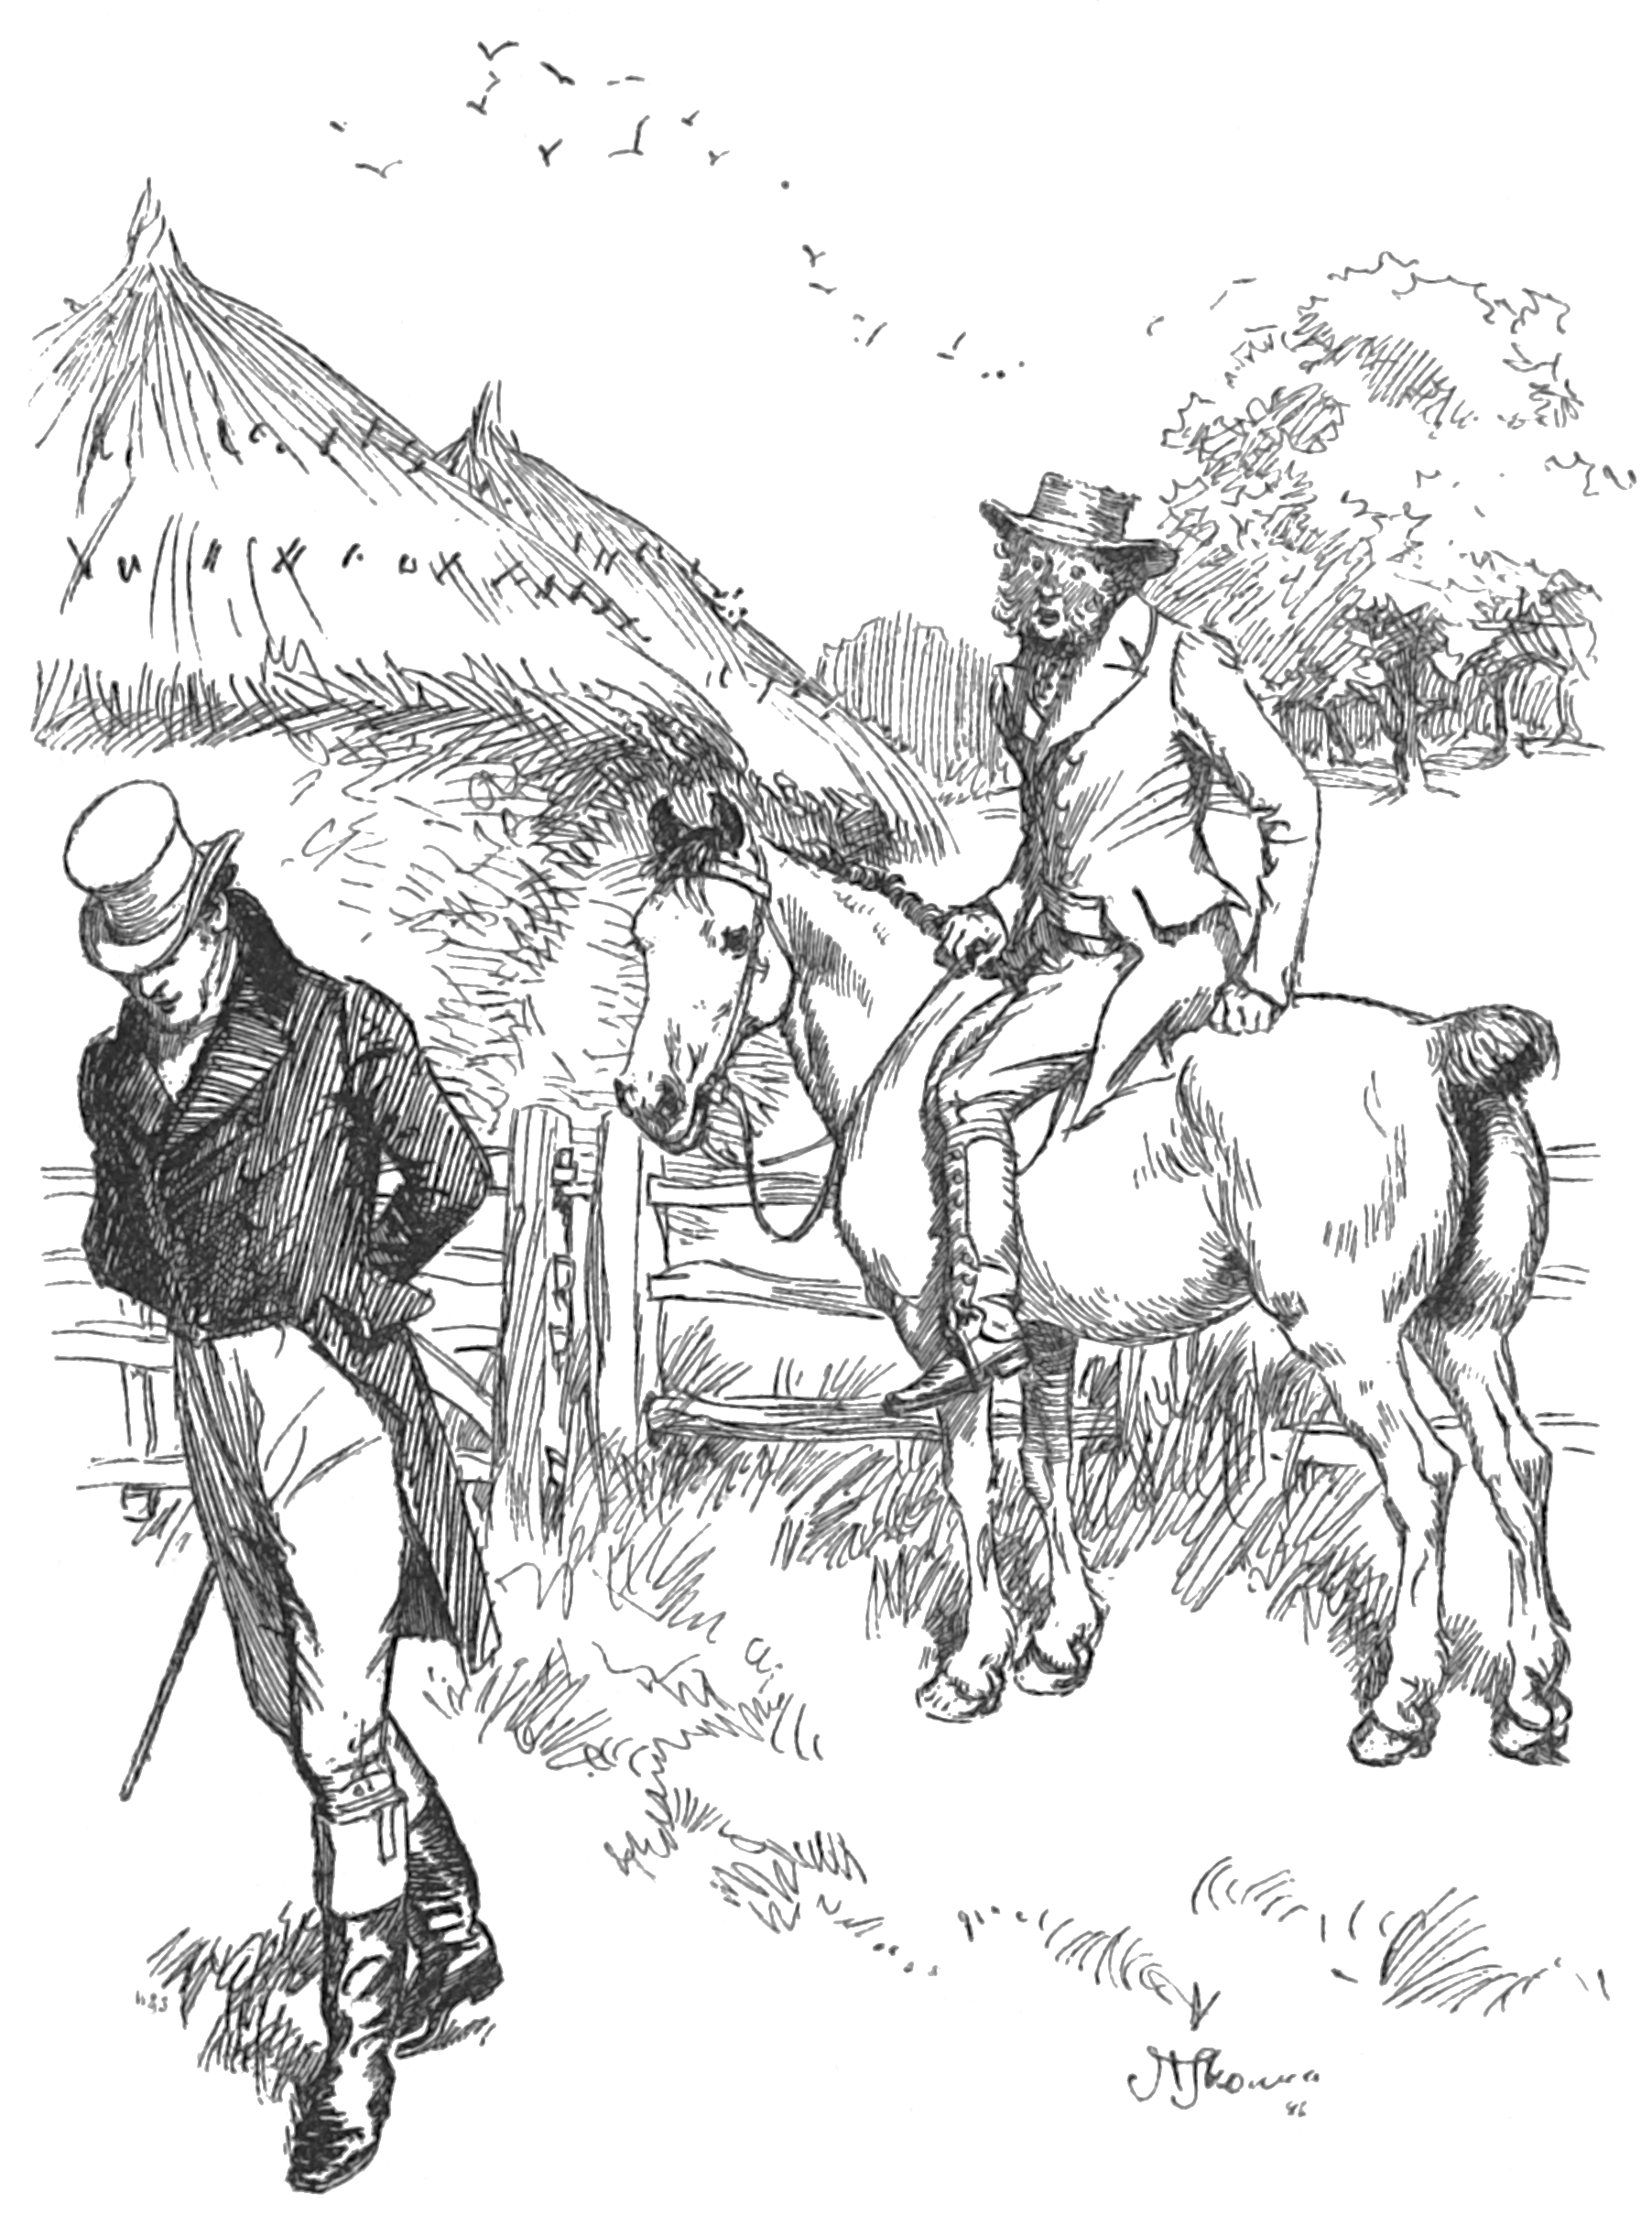
\includegraphics[width=\linewidth]{51walking}
\caption{Walking away from William Larkins}
\end{figure}

Of their all removing to Donwell, Emma had already had her own passing thoughts. Like him, she had tried the scheme and rejected it; but such an alternative as this had not occurred to her. She was sensible of all the affection it evinced. She felt that, in quitting Donwell, he must be sacrificing a great deal of independence of hours and habits; that in living constantly with her father, and in no house of his own, there would be much, very much, to be borne with. She promised to think of it, and advised him to think of it more; but he was fully convinced, that no reflection could alter his wishes or his opinion on the subject. He had given it, he could assure her, very long and calm consideration; he had been walking away from William Larkins the whole morning, to have his thoughts to himself.

»Ah! there is one difficulty unprovided for,« cried Emma. »I am sure William Larkins will not like it. You must get his consent before you ask mine.«

She promised, however, to think of it; and pretty nearly promised, moreover, to think of it, with the intention of finding it a very good scheme.

It is remarkable, that Emma, in the many, very many, points of view in which she was now beginning to consider Donwell Abbey, was never struck with any sense of injury to her nephew Henry, whose rights as heir-expectant had formerly been so tenaciously regarded. Think she must of the possible difference to the poor little boy; and yet she only gave herself a saucy conscious smile about it, and found amusement in detecting the real cause of that violent dislike of Mr Knightley's marrying Jane Fairfax, or any body else, which at the time she had wholly imputed to the amiable solicitude of the sister and the aunt.

This proposal of his, this plan of marrying and continuing at Hartfield—the more she contemplated it, the more pleasing it became. His evils seemed to lessen, her own advantages to increase, their mutual good to outweigh every drawback. Such a companion for herself in the periods of anxiety and cheerlessness before her!—Such a partner in all those duties and cares to which time must be giving increase of melancholy!

She would have been too happy but for poor Harriet; but every blessing of her own seemed to involve and advance the sufferings of her friend, who must now be even excluded from Hartfield. The delightful family party which Emma was securing for herself, poor Harriet must, in mere charitable caution, be kept at a distance from. She would be a loser in every way. Emma could not deplore her future absence as any deduction from her own enjoyment. In such a party, Harriet would be rather a dead weight than otherwise; but for the poor girl herself, it seemed a peculiarly cruel necessity that was to be placing her in such a state of unmerited punishment.

In time, of course, Mr Knightley would be forgotten, that is, supplanted; but this could not be expected to happen very early. Mr Knightley himself would be doing nothing to assist the cure;—not like Mr Elton. Mr Knightley, always so kind, so feeling, so truly considerate for every body, would never deserve to be less worshipped than now; and it really was too much to hope even of Harriet, that she could be in love with more than three men in one year.
%!TeX root=../emmatop.tex
\chapter[Chapter \thechapter]{}
\lettrine[lines=4,lraise=0.3]{I}{t} was a very great relief to Emma to find Harriet as desirous as herself to avoid a meeting. Their intercourse was painful enough by letter. How much worse, had they been obliged to meet!

\zz
Harriet expressed herself very much as might be supposed, without reproaches, or apparent sense of ill-usage; and yet Emma fancied there was a something of resentment, a something bordering on it in her style, which increased the desirableness of their being separate.—It might be only her own consciousness; but it seemed as if an angel only could have been quite without resentment under such a stroke.

She had no difficulty in procuring Isabella's invitation; and she was fortunate in having a sufficient reason for asking it, without resorting to invention.—There was a tooth amiss. Harriet really wished, and had wished some time, to consult a dentist. Mrs John Knightley was delighted to be of use; any thing of ill health was a recommendation to her—and though not so fond of a dentist as of a Mr Wingfield, she was quite eager to have Harriet under her care.—When it was thus settled on her sister's side, Emma proposed it to her friend, and found her very persuadable.—Harriet was to go; she was invited for at least a fortnight; she was to be conveyed in Mr Woodhouse's carriage.—It was all arranged, it was all completed, and Harriet was safe in Brunswick Square.

Now Emma could, indeed, enjoy Mr Knightley's visits; now she could talk, and she could listen with true happiness, unchecked by that sense of injustice, of guilt, of something most painful, which had haunted her when remembering how disappointed a heart was near her, how much might at that moment, and at a little distance, be enduring by the feelings which she had led astray herself.

The difference of Harriet at Mrs Goddard's, or in London, made perhaps an unreasonable difference in Emma's sensations; but she could not think of her in London without objects of curiosity and employment, which must be averting the past, and carrying her out of herself.

She would not allow any other anxiety to succeed directly to the place in her mind which Harriet had occupied. There was a communication before her, one which she only could be competent to make—the confession of her engagement to her father; but she would have nothing to do with it at present.—She had resolved to defer the disclosure till Mrs Weston were safe and well. No additional agitation should be thrown at this period among those she loved—and the evil should not act on herself by anticipation before the appointed time.—A fortnight, at least, of leisure and peace of mind, to crown every warmer, but more agitating, delight, should be hers.

She soon resolved, equally as a duty and a pleasure, to employ half an hour of this holiday of spirits in calling on Miss Fairfax.—She ought to go—and she was longing to see her; the resemblance of their present situations increasing every other motive of goodwill. It would be a secret satisfaction; but the consciousness of a similarity of prospect would certainly add to the interest with which she should attend to any thing Jane might communicate.

She went—she had driven once unsuccessfully to the door, but had not been into the house since the morning after Box Hill, when poor Jane had been in such distress as had filled her with compassion, though all the worst of her sufferings had been unsuspected.—The fear of being still unwelcome, determined her, though assured of their being at home, to wait in the passage, and send up her name.—She heard Patty announcing it; but no such bustle succeeded as poor Miss Bates had before made so happily intelligible.—No; she heard nothing but the instant reply of, »Beg her to walk up;«—and a moment afterwards she was met on the stairs by Jane herself, coming eagerly forward, as if no other reception of her were felt sufficient.—Emma had never seen her look so well, so lovely, so engaging. There was consciousness, animation, and warmth; there was every thing which her countenance or manner could ever have wanted.— She came forward with an offered hand; and said, in a low, but very feeling tone,

»This is most kind, indeed!—Miss Woodhouse, it is impossible for me to express—I hope you will believe—Excuse me for being so entirely without words.«

Emma was gratified, and would soon have shewn no want of words, if the sound of Mrs Elton's voice from the sitting-room had not checked her, and made it expedient to compress all her friendly and all her congratulatory sensations into a very, very earnest shake of the hand.

Mrs Bates and Mrs Elton were together. Miss Bates was out, which accounted for the previous tranquillity. Emma could have wished Mrs Elton elsewhere; but she was in a humour to have patience with every body; and as Mrs Elton met her with unusual graciousness, she hoped the rencontre would do them no harm.

She soon believed herself to penetrate Mrs Elton's thoughts, and understand why she was, like herself, in happy spirits; it was being in Miss Fairfax's confidence, and fancying herself acquainted with what was still a secret to other people. Emma saw symptoms of it immediately in the expression of her face; and while paying her own compliments to Mrs Bates, and appearing to attend to the good old lady's replies, she saw her with a sort of anxious parade of mystery fold up a letter which she had apparently been reading aloud to Miss Fairfax, and return it into the purple and gold reticule by her side, saying, with significant nods,

»We can finish this some other time, you know. You and I shall not want opportunities. And, in fact, you have heard all the essential already. I only wanted to prove to you that Mrs S. admits our apology, and is not offended. You see how delightfully she writes. Oh! she is a sweet creature! You would have doated on her, had you gone.—But not a word more. Let us be discreet—quite on our good behaviour.—Hush!—You remember those lines—I forget the poem at this moment:

\begin{verse}
For when a lady's in the case,\\
You know all other things give place.
\end{verse}


Now I say, my dear, in our case, for lady, read——mum! a word to the wise.—I am in a fine flow of spirits, an't I? But I want to set your heart at ease as to Mrs S.—My representation, you see, has quite appeased her.«

And again, on Emma's merely turning her head to look at Mrs Bates's knitting, she added, in a half whisper,

»I mentioned no names, you will observe.—Oh! no; cautious as a minister of state. I managed it extremely well.«

Emma could not doubt. It was a palpable display, repeated on every possible occasion. When they had all talked a little while in harmony of the weather and Mrs Weston, she found herself abruptly addressed with,

»Do not you think, Miss Woodhouse, our saucy little friend here is charmingly recovered?—Do not you think her cure does Perry the highest credit?—(here was a side-glance of great meaning at Jane.) Upon my word, Perry has restored her in a wonderful short time!—Oh! if you had seen her, as I did, when she was at the worst!«—And when Mrs Bates was saying something to Emma, whispered farther, »We do not say a word of any assistance that Perry might have; not a word of a certain young physician from Windsor.—Oh! no; Perry shall have all the credit.«

»I have scarce had the pleasure of seeing you, Miss Woodhouse,« she shortly afterwards began, »since the party to Box Hill. Very pleasant party. But yet I think there was something wanting. Things did not seem—that is, there seemed a little cloud upon the spirits of some.—So it appeared to me at least, but I might be mistaken. However, I think it answered so far as to tempt one to go again. What say you both to our collecting the same party, and exploring to Box Hill again, while the fine weather lasts?—It must be the same party, you know, quite the same party, not one exception.«

Soon after this Miss Bates came in, and Emma could not help being diverted by the perplexity of her first answer to herself, resulting, she supposed, from doubt of what might be said, and impatience to say every thing.

»Thank you, dear Miss Woodhouse, you are all kindness.—It is impossible to say—Yes, indeed, I quite understand—dearest Jane's prospects—that is, I do not mean.—But she is charmingly recovered.—How is Mr Woodhouse?—I am so glad.—Quite out of my power.—Such a happy little circle as you find us here.—Yes, indeed.—Charming young man!—that is—so very friendly; I mean good Mr Perry!—such attention to Jane!«—And from her great, her more than commonly thankful delight towards Mrs Elton for being there, Emma guessed that there had been a little show of resentment towards Jane, from the vicarage quarter, which was now graciously overcome.—After a few whispers, indeed, which placed it beyond a guess, Mrs Elton, speaking louder, said,

»Yes, here I am, my good friend; and here I have been so long, that anywhere else I should think it necessary to apologise; but, the truth is, that I am waiting for my lord and master. He promised to join me here, and pay his respects to you.«

»What! are we to have the pleasure of a call from Mr Elton?—That will be a favour indeed! for I know gentlemen do not like morning visits, and Mr Elton's time is so engaged.«

»Upon my word it is, Miss Bates.—He really is engaged from morning to night.—There is no end of people's coming to him, on some pretence or other.—The magistrates, and overseers, and churchwardens, are always wanting his opinion. They seem not able to do any thing without him.—»Upon my word, Mr E.,« I often say, »rather you than I.—I do not know what would become of my crayons and my instrument, if I had half so many applicants.«—Bad enough as it is, for I absolutely neglect them both to an unpardonable degree.—I believe I have not played a bar this fortnight.—However, he is coming, I assure you: yes, indeed, on purpose to wait on you all.« And putting up her hand to screen her words from Emma—»A congratulatory visit, you know.—Oh! yes, quite indispensable.«

Miss Bates looked about her, so happily—!

»He promised to come to me as soon as he could disengage himself from Knightley; but he and Knightley are shut up together in deep consultation.—Mr E. is Knightley's right hand.«

Emma would not have smiled for the world, and only said, »Is Mr Elton gone on foot to Donwell?—He will have a hot walk.«

»Oh! no, it is a meeting at the Crown, a regular meeting. Weston and Cole will be there too; but one is apt to speak only of those who lead.—I fancy Mr E. and Knightley have every thing their own way.«

»Have not you mistaken the day?« said Emma. »I am almost certain that the meeting at the Crown is not till to-morrow.—Mr Knightley was at Hartfield yesterday, and spoke of it as for Saturday.«

»Oh! no, the meeting is certainly to-day,« was the abrupt answer, which denoted the impossibility of any blunder on Mrs Elton's side.—»I do believe,« she continued, »this is the most troublesome parish that ever was. We never heard of such things at Maple Grove.«

»Your parish there was small,« said Jane.

»Upon my word, my dear, I do not know, for I never heard the subject talked of.«

»But it is proved by the smallness of the school, which I have heard you speak of, as under the patronage of your sister and Mrs Bragge; the only school, and not more than five-and-twenty children.«

»Ah! you clever creature, that's very true. What a thinking brain you have! I say, Jane, what a perfect character you and I should make, if we could be shaken together. My liveliness and your solidity would produce perfection.—Not that I presume to insinuate, however, that some people may not think you perfection already.—But hush!—not a word, if you please.«

It seemed an unnecessary caution; Jane was wanting to give her words, not to Mrs Elton, but to Miss Woodhouse, as the latter plainly saw. The wish of distinguishing her, as far as civility permitted, was very evident, though it could not often proceed beyond a look.

Mr Elton made his appearance. His lady greeted him with some of her sparkling vivacity.

»Very pretty, sir, upon my word; to send me on here, to be an encumbrance to my friends, so long before you vouchsafe to come!—But you knew what a dutiful creature you had to deal with. You knew I should not stir till my lord and master appeared.—Here have I been sitting this hour, giving these young ladies a sample of true conjugal obedience—for who can say, you know, how soon it may be wanted?«

Mr Elton was so hot and tired, that all this wit seemed thrown away. His civilities to the other ladies must be paid; but his subsequent object was to lament over himself for the heat he was suffering, and the walk he had had for nothing.

»When I got to Donwell,« said he, »Knightley could not be found. Very odd! very unaccountable! after the note I sent him this morning, and the message he returned, that he should certainly be at home till one.«

»Donwell!« cried his wife.—»My dear Mr E., you have not been to Donwell!—You mean the Crown; you come from the meeting at the Crown.«

\begin{figure}[tbph]
\centering
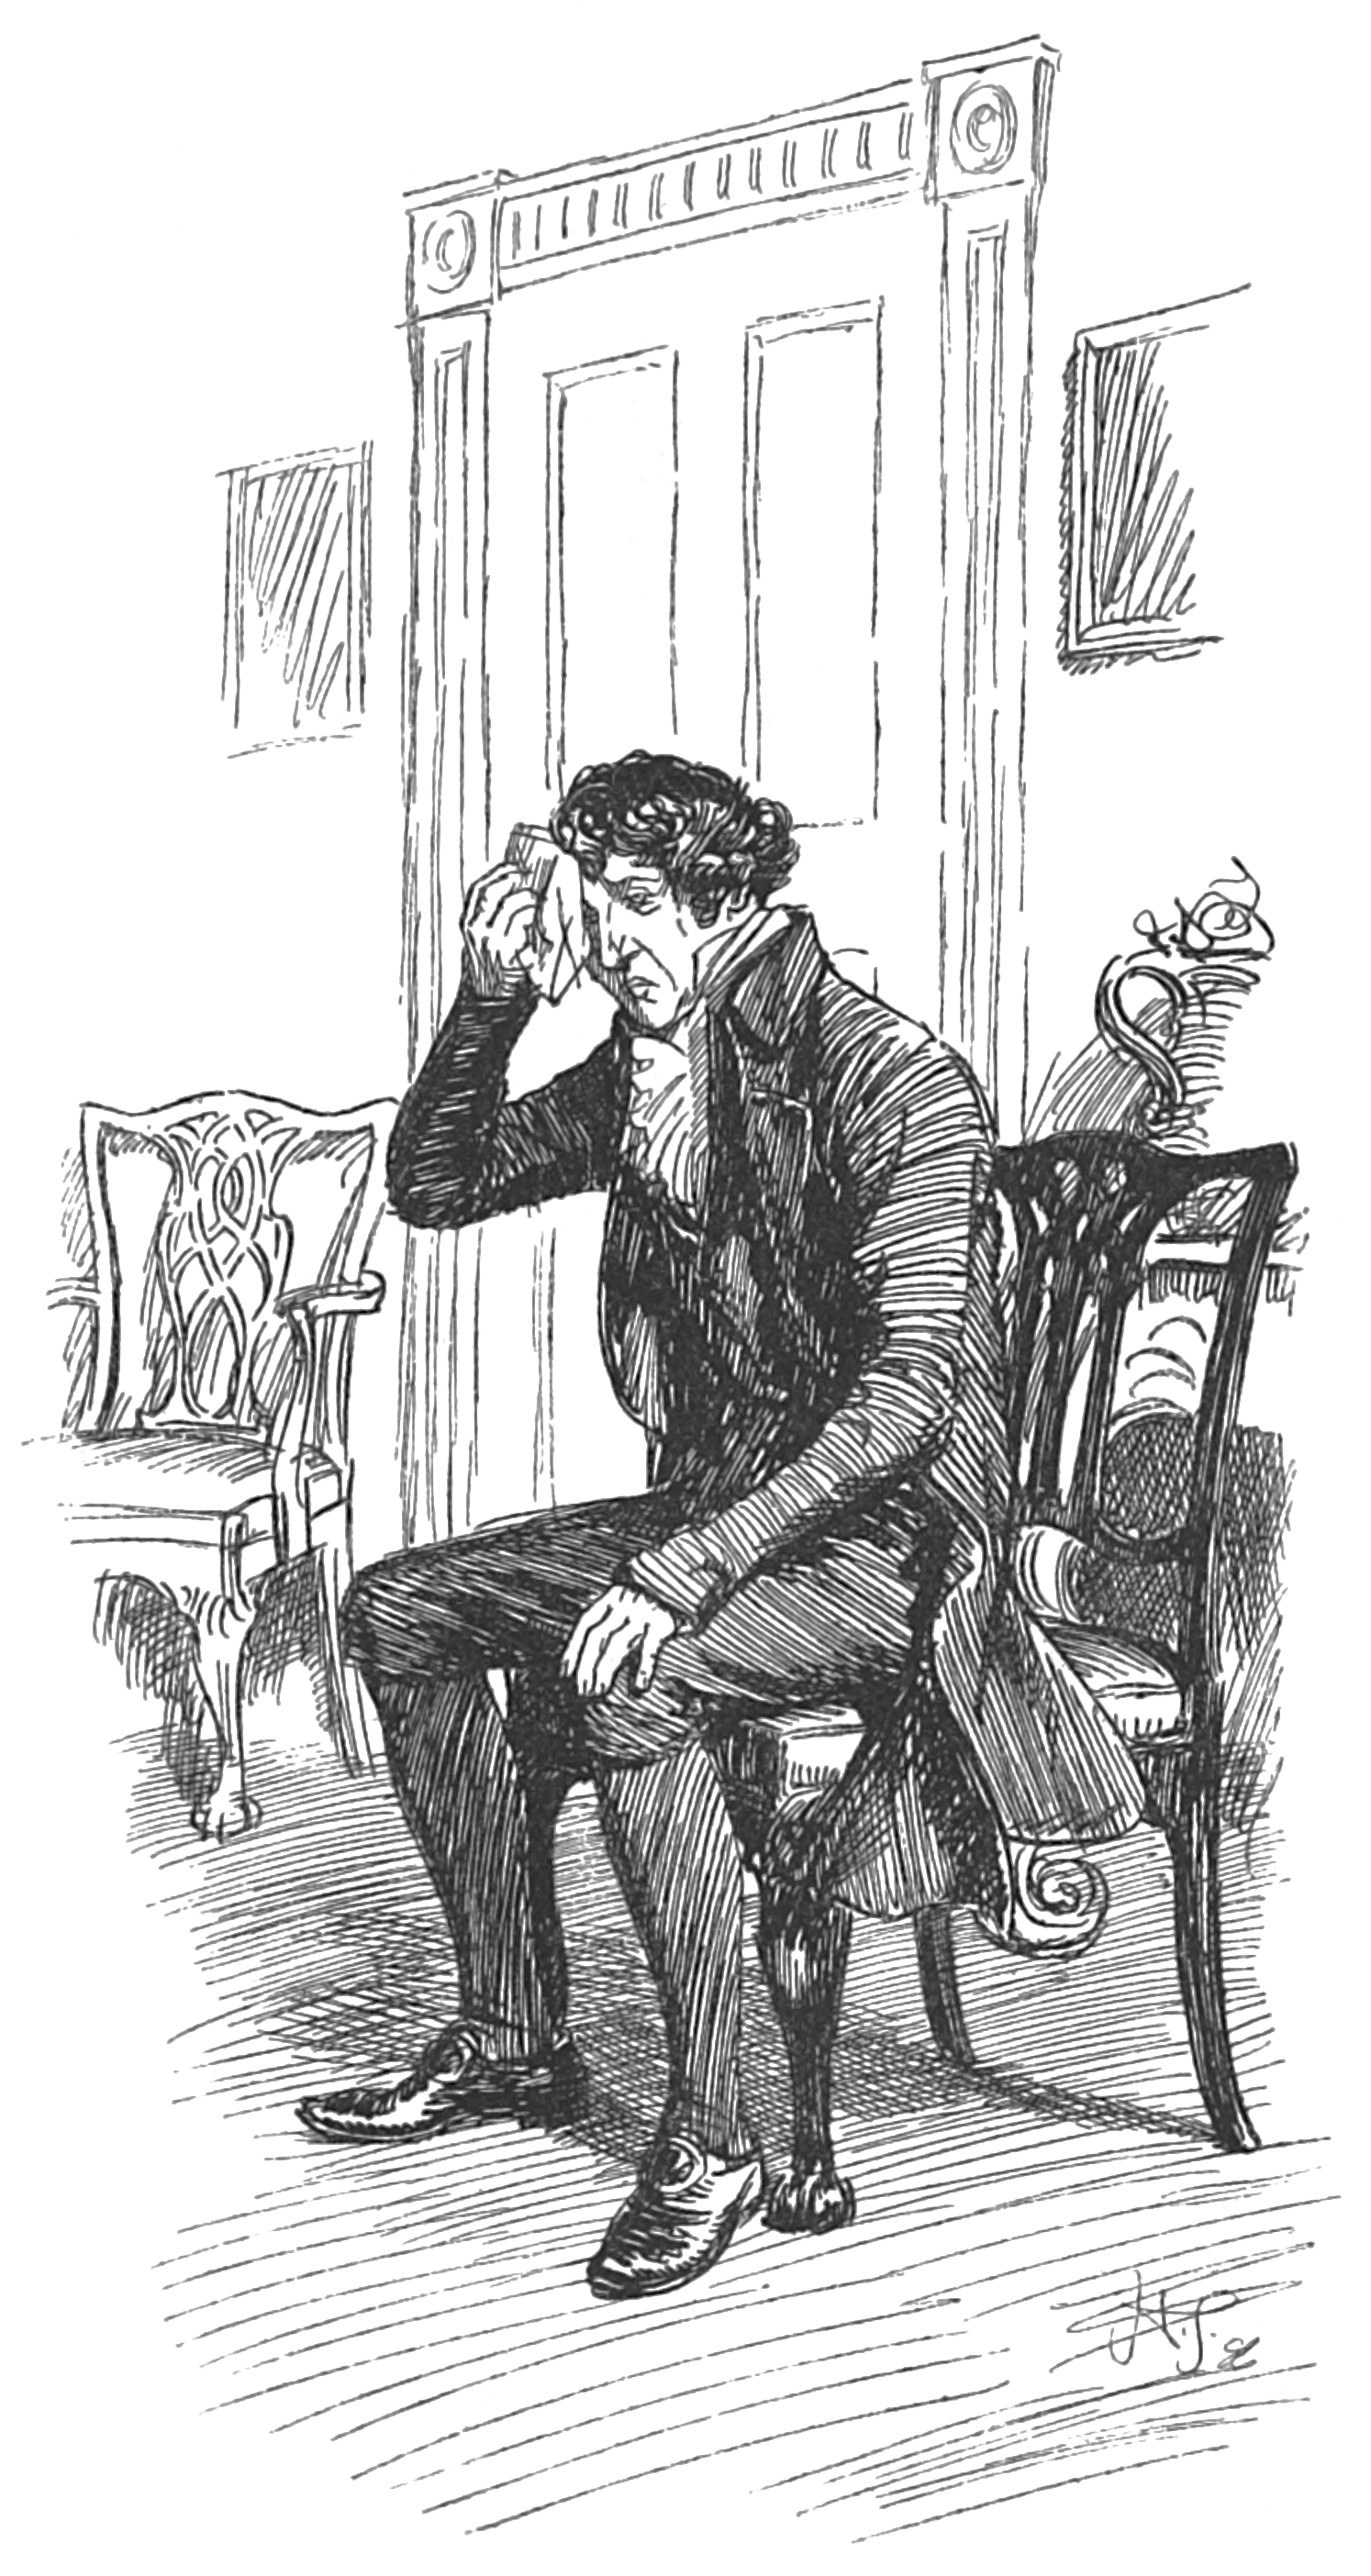
\includegraphics[width=.8\linewidth]{52broiling}
\caption{»Such a dreadful broiling morning!«}
\end{figure}

»No, no, that's to-morrow; and I particularly wanted to see Knightley to-day on that very account.—Such a dreadful broiling morning!—I went over the fields too—(speaking in a tone of great ill-usage,) which made it so much the worse. And then not to find him at home! I assure you I am not at all pleased. And no apology left, no message for me. The housekeeper declared she knew nothing of my being expected.—Very extraordinary!—And nobody knew at all which way he was gone. Perhaps to Hartfield, perhaps to the Abbey Mill, perhaps into his woods.—Miss Woodhouse, this is not like our friend Knightley!—Can you explain it?«

Emma amused herself by protesting that it was very extraordinary, indeed, and that she had not a syllable to say for him.

»I cannot imagine,« said Mrs Elton, (feeling the indignity as a wife ought to do,) »I cannot imagine how he could do such a thing by you, of all people in the world! The very last person whom one should expect to be forgotten!—My dear Mr E., he must have left a message for you, I am sure he must.—Not even Knightley could be so very eccentric;—and his servants forgot it. Depend upon it, that was the case: and very likely to happen with the Donwell servants, who are all, I have often observed, extremely awkward and remiss.—I am sure I would not have such a creature as his Harry stand at our sideboard for any consideration. And as for Mrs Hodges, Wright holds her very cheap indeed.—She promised Wright a receipt, and never sent it.«

»I met William Larkins,« continued Mr Elton, »as I got near the house, and he told me I should not find his master at home, but I did not believe him.—William seemed rather out of humour. He did not know what was come to his master lately, he said, but he could hardly ever get the speech of him. I have nothing to do with William's wants, but it really is of very great importance that I should see Knightley to-day; and it becomes a matter, therefore, of very serious inconvenience that I should have had this hot walk to no purpose.«

Emma felt that she could not do better than go home directly. In all probability she was at this very time waited for there; and Mr Knightley might be preserved from sinking deeper in aggression towards Mr Elton, if not towards William Larkins.

She was pleased, on taking leave, to find Miss Fairfax determined to attend her out of the room, to go with her even downstairs; it gave her an opportunity which she immediately made use of, to say,

»It is as well, perhaps, that I have not had the possibility. Had you not been surrounded by other friends, I might have been tempted to introduce a subject, to ask questions, to speak more openly than might have been strictly correct.—I feel that I should certainly have been impertinent.«

»Oh!« cried Jane, with a blush and an hesitation which Emma thought infinitely more becoming to her than all the elegance of all her usual composure—»there would have been no danger. The danger would have been of my wearying you. You could not have gratified me more than by expressing an interest—. Indeed, Miss Woodhouse, (speaking more collectedly,) with the consciousness which I have of misconduct, very great misconduct, it is particularly consoling to me to know that those of my friends, whose good opinion is most worth preserving, are not disgusted to such a degree as to—I have not time for half that I could wish to say. I long to make apologies, excuses, to urge something for myself. I feel it so very due. But, unfortunately—in short, if your compassion does not stand my friend—«

»Oh! you are too scrupulous, indeed you are,« cried Emma warmly, and taking her hand. »You owe me no apologies; and every body to whom you might be supposed to owe them, is so perfectly satisfied, so delighted even\longdash«

»You are very kind, but I know what my manners were to you.—So cold and artificial!—I had always a part to act.—It was a life of deceit!—I know that I must have disgusted you.«

»Pray say no more. I feel that all the apologies should be on my side. Let us forgive each other at once. We must do whatever is to be done quickest, and I think our feelings will lose no time there. I hope you have pleasant accounts from Windsor?«

»Very.«

»And the next news, I suppose, will be, that we are to lose you—just as I begin to know you.«

»Oh! as to all that, of course nothing can be thought of yet. I am here till claimed by Colonel and Mrs Campbell.«

»Nothing can be actually settled yet, perhaps,« replied Emma, smiling—»but, excuse me, it must be thought of.«

The smile was returned as Jane answered,

»You are very right; it has been thought of. And I will own to you, (I am sure it will be safe), that so far as our living with Mr Churchill at Enscombe, it is settled. There must be three months, at least, of deep mourning; but when they are over, I imagine there will be nothing more to wait for.«

»Thank you, thank you.—This is just what I wanted to be assured of.—Oh! if you knew how much I love every thing that is decided and open!—Good-bye, good-bye.«
%!TeX root=../emmatop.tex
\chapter[Chapter \thechapter]{}
\lettrine[lines=4,lraise=0.3]{M}{rs} Weston's friends were all made happy by her safety; and if the satisfaction of her well-doing could be increased to Emma, it was by knowing her to be the mother of a little girl. She had been decided in wishing for a Miss Weston. She would not acknowledge that it was with any view of making a match for her, hereafter, with either of Isabella's sons; but she was convinced that a daughter would suit both father and mother best. It would be a great comfort to Mr Weston, as he grew older—and even Mr Weston might be growing older ten years hence—to have his fireside enlivened by the sports and the nonsense, the freaks and the fancies of a child never banished from home; and Mrs Weston—no one could doubt that a daughter would be most to her; and it would be quite a pity that any one who so well knew how to teach, should not have their powers in exercise again.

»She has had the advantage, you know, of practising on me,« she continued—»like La Baronne d'Almane on La Comtesse d'Ostalis, in Madame de Genlis' Adelaide and Theodore, and we shall now see her own little Adelaide educated on a more perfect plan.«

»That is,« replied Mr Knightley, »she will indulge her even more than she did you, and believe that she does not indulge her at all. It will be the only difference.«

»Poor child!« cried Emma; »at that rate, what will become of her?«

»Nothing very bad.—The fate of thousands. She will be disagreeable in infancy, and correct herself as she grows older. I am losing all my bitterness against spoilt children, my dearest Emma. I, who am owing all my happiness to you, would not it be horrible ingratitude in me to be severe on them?«

Emma laughed, and replied: »But I had the assistance of all your endeavours to counteract the indulgence of other people. I doubt whether my own sense would have corrected me without it.«

»Do you?—I have no doubt. Nature gave you understanding:—Miss Taylor gave you principles. You must have done well. My interference was quite as likely to do harm as good. It was very natural for you to say, what right has he to lecture me?—and I am afraid very natural for you to feel that it was done in a disagreeable manner. I do not believe I did you any good. The good was all to myself, by making you an object of the tenderest affection to me. I could not think about you so much without doating on you, faults and all; and by dint of fancying so many errors, have been in love with you ever since you were thirteen at least.«

»I am sure you were of use to me,« cried Emma. »I was very often influenced rightly by you—oftener than I would own at the time. I am very sure you did me good. And if poor little Anna Weston is to be spoiled, it will be the greatest humanity in you to do as much for her as you have done for me, except falling in love with her when she is thirteen.«

»How often, when you were a girl, have you said to me, with one of your saucy looks—»Mr Knightley, I am going to do so-and-so; papa says I may, or I have Miss Taylor's leave«—something which, you knew, I did not approve. In such cases my interference was giving you two bad feelings instead of one.«

»What an amiable creature I was!—No wonder you should hold my speeches in such affectionate remembrance.«

»»Mr Knightley.«—You always called me, »Mr Knightley;« and, from habit, it has not so very formal a sound.—And yet it is formal. I want you to call me something else, but I do not know what.«

»I remember once calling you »George,« in one of my amiable fits, about ten years ago. I did it because I thought it would offend you; but, as you made no objection, I never did it again.«

»And cannot you call me »George« now?«

»Impossible!—I never can call you any thing but »Mr Knightley.« I will not promise even to equal the elegant terseness of Mrs Elton, by calling you Mr K.—But I will promise,« she added presently, laughing and blushing—»I will promise to call you once by your Christian name. I do not say when, but perhaps you may guess where;—in the building in which N. takes M. for better, for worse.«

Emma grieved that she could not be more openly just to one important service which his better sense would have rendered her, to the advice which would have saved her from the worst of all her womanly follies—her wilful intimacy with Harriet Smith; but it was too tender a subject.—She could not enter on it.—Harriet was very seldom mentioned between them. This, on his side, might merely proceed from her not being thought of; but Emma was rather inclined to attribute it to delicacy, and a suspicion, from some appearances, that their friendship were declining. She was aware herself, that, parting under any other circumstances, they certainly should have corresponded more, and that her intelligence would not have rested, as it now almost wholly did, on Isabella's letters. He might observe that it was so. The pain of being obliged to practise concealment towards him, was very little inferior to the pain of having made Harriet unhappy.

Isabella sent quite as good an account of her visitor as could be expected; on her first arrival she had thought her out of spirits, which appeared perfectly natural, as there was a dentist to be consulted; but, since that business had been over, she did not appear to find Harriet different from what she had known her before.—Isabella, to be sure, was no very quick observer; yet if Harriet had not been equal to playing with the children, it would not have escaped her. Emma's comforts and hopes were most agreeably carried on, by Harriet's being to stay longer; her fortnight was likely to be a month at least. Mr and Mrs John Knightley were to come down in August, and she was invited to remain till they could bring her back.

»John does not even mention your friend,« said Mr Knightley. »Here is his answer, if you like to see it.«

It was the answer to the communication of his intended marriage. Emma accepted it with a very eager hand, with an impatience all alive to know what he would say about it, and not at all checked by hearing that her friend was unmentioned.

»John enters like a brother into my happiness,« continued Mr Knightley, »but he is no complimenter; and though I well know him to have, likewise, a most brotherly affection for you, he is so far from making flourishes, that any other young woman might think him rather cool in her praise. But I am not afraid of your seeing what he writes.«

»He writes like a sensible man,« replied Emma, when she had read the letter. »I honour his sincerity. It is very plain that he considers the good fortune of the engagement as all on my side, but that he is not without hope of my growing, in time, as worthy of your affection, as you think me already. Had he said any thing to bear a different construction, I should not have believed him.«

»My Emma, he means no such thing. He only means\longdash«

»He and I should differ very little in our estimation of the two,« interrupted she, with a sort of serious smile—»much less, perhaps, than he is aware of, if we could enter without ceremony or reserve on the subject.«

»Emma, my dear Emma\longdash«

»Oh!« she cried with more thorough gaiety, »if you fancy your brother does not do me justice, only wait till my dear father is in the secret, and hear his opinion. Depend upon it, he will be much farther from doing you justice. He will think all the happiness, all the advantage, on your side of the question; all the merit on mine. I wish I may not sink into »poor Emma« with him at once.—His tender compassion towards oppressed worth can go no farther.«

»Ah!« he cried, »I wish your father might be half as easily convinced as John will be, of our having every right that equal worth can give, to be happy together. I am amused by one part of John's letter—did you notice it?—where he says, that my information did not take him wholly by surprize, that he was rather in expectation of hearing something of the kind.«

»If I understand your brother, he only means so far as your having some thoughts of marrying. He had no idea of me. He seems perfectly unprepared for that.«

»Yes, yes—but I am amused that he should have seen so far into my feelings. What has he been judging by?—I am not conscious of any difference in my spirits or conversation that could prepare him at this time for my marrying any more than at another.—But it was so, I suppose. I dare say there was a difference when I was staying with them the other day. I believe I did not play with the children quite so much as usual. I remember one evening the poor boys saying, »Uncle seems always tired now.««

The time was coming when the news must spread farther, and other persons' reception of it tried. As soon as Mrs Weston was sufficiently recovered to admit Mr Woodhouse's visits, Emma having it in view that her gentle reasonings should be employed in the cause, resolved first to announce it at home, and then at Randalls.—But how to break it to her father at last!—She had bound herself to do it, in such an hour of Mr Knightley's absence, or when it came to the point her heart would have failed her, and she must have put it off; but Mr Knightley was to come at such a time, and follow up the beginning she was to make.—She was forced to speak, and to speak cheerfully too. She must not make it a more decided subject of misery to him, by a melancholy tone herself. She must not appear to think it a misfortune.—With all the spirits she could command, she prepared him first for something strange, and then, in a few words, said, that if his consent and approbation could be obtained—which, she trusted, would be attended with no difficulty, since it was a plan to promote the happiness of all—she and Mr Knightley meant to marry; by which means Hartfield would receive the constant addition of that person's company whom she knew he loved, next to his daughters and Mrs Weston, best in the world.

\begin{figure}[tbph]
\centering
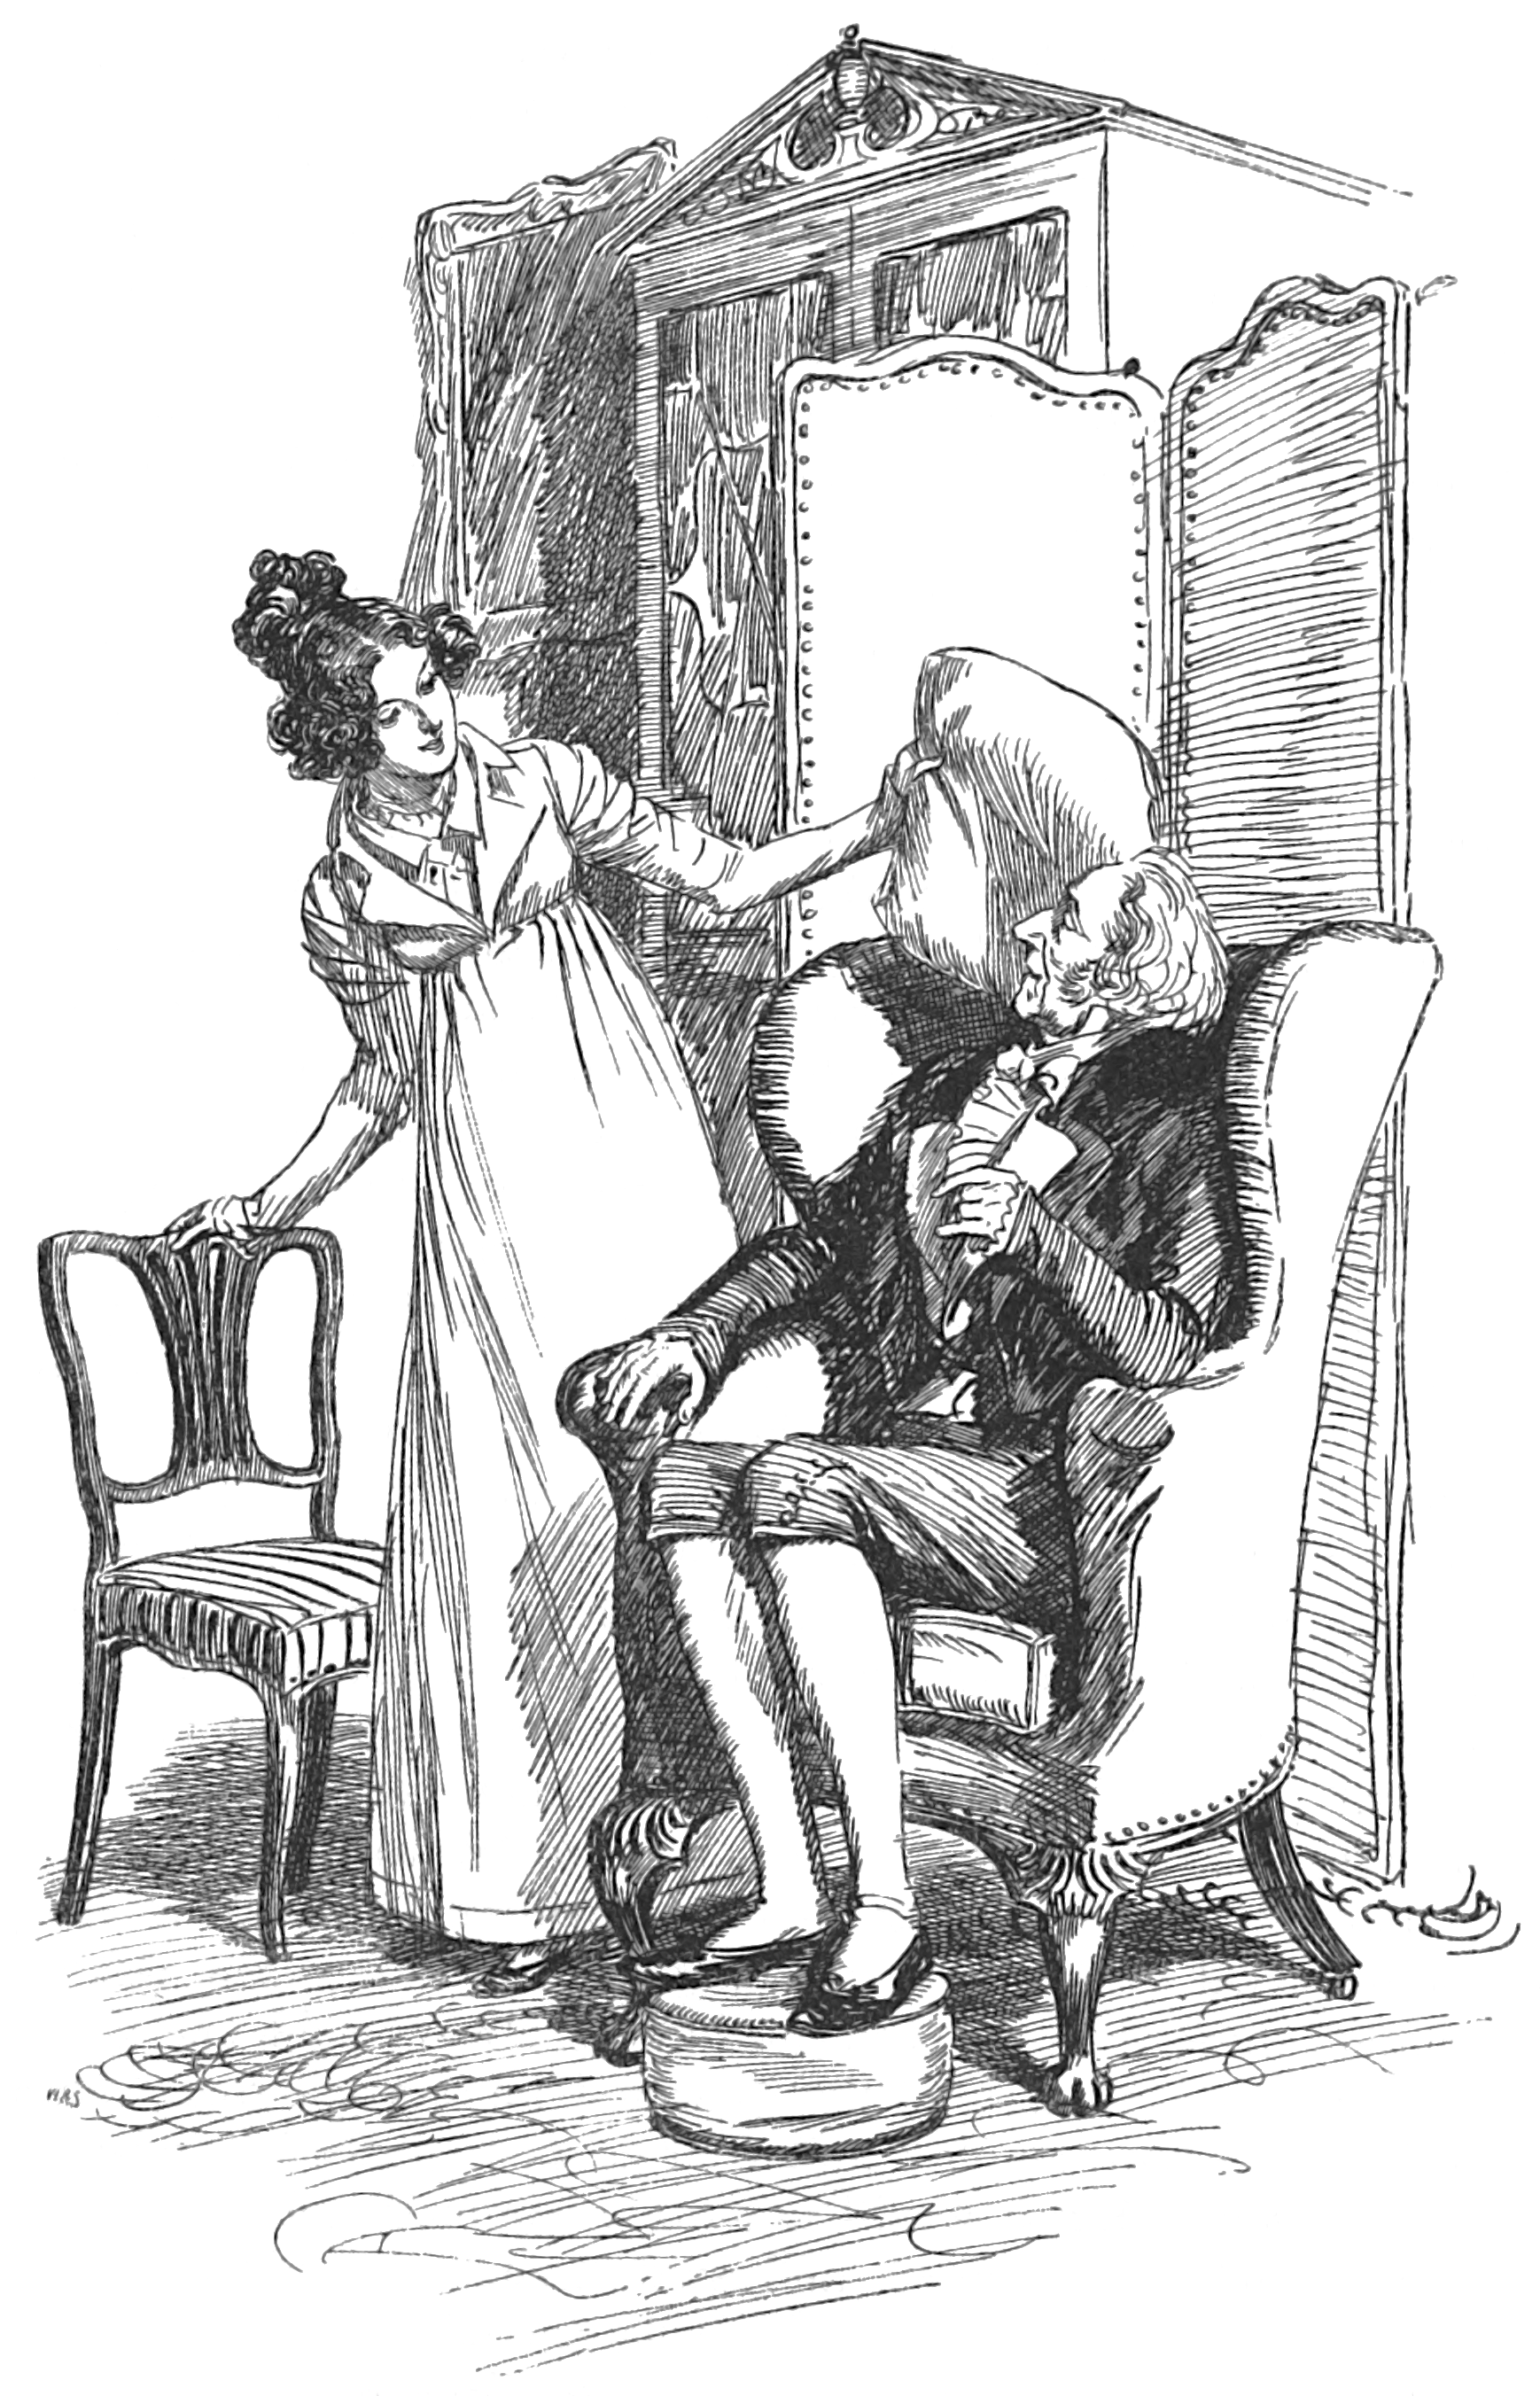
\includegraphics[width=\linewidth]{53affectionately}
\caption{Emma hung about him affectionately}
\end{figure}

Poor man!—it was at first a considerable shock to him, and he tried earnestly to dissuade her from it. She was reminded, more than once, of having always said she would never marry, and assured that it would be a great deal better for her to remain single; and told of poor Isabella, and poor Miss Taylor.—But it would not do. Emma hung about him affectionately, and smiled, and said it must be so; and that he must not class her with Isabella and Mrs Weston, whose marriages taking them from Hartfield, had, indeed, made a melancholy change: but she was not going from Hartfield; she should be always there; she was introducing no change in their numbers or their comforts but for the better; and she was very sure that he would be a great deal the happier for having Mr Knightley always at hand, when he were once got used to the idea.—Did he not love Mr Knightley very much?—He would not deny that he did, she was sure.—Whom did he ever want to consult on business but Mr Knightley?—Who was so useful to him, who so ready to write his letters, who so glad to assist him?—Who so cheerful, so attentive, so attached to him?—Would not he like to have him always on the spot?—Yes. That was all very true. Mr Knightley could not be there too often; he should be glad to see him every day;—but they did see him every day as it was.—Why could not they go on as they had done?

Mr Woodhouse could not be soon reconciled; but the worst was overcome, the idea was given; time and continual repetition must do the rest.—To Emma's entreaties and assurances succeeded Mr Knightley's, whose fond praise of her gave the subject even a kind of welcome; and he was soon used to be talked to by each, on every fair occasion.—They had all the assistance which Isabella could give, by letters of the strongest approbation; and Mrs Weston was ready, on the first meeting, to consider the subject in the most serviceable light—first, as a settled, and, secondly, as a good one—well aware of the nearly equal importance of the two recommendations to Mr Woodhouse's mind.—It was agreed upon, as what was to be; and every body by whom he was used to be guided assuring him that it would be for his happiness; and having some feelings himself which almost admitted it, he began to think that some time or other—in another year or two, perhaps—it might not be so very bad if the marriage did take place.

Mrs Weston was acting no part, feigning no feelings in all that she said to him in favour of the event.—She had been extremely surprized, never more so, than when Emma first opened the affair to her; but she saw in it only increase of happiness to all, and had no scruple in urging him to the utmost.—She had such a regard for Mr Knightley, as to think he deserved even her dearest Emma; and it was in every respect so proper, suitable, and unexceptionable a connexion, and in one respect, one point of the highest importance, so peculiarly eligible, so singularly fortunate, that now it seemed as if Emma could not safely have attached herself to any other creature, and that she had herself been the stupidest of beings in not having thought of it, and wished it long ago.—How very few of those men in a rank of life to address Emma would have renounced their own home for Hartfield! And who but Mr Knightley could know and bear with Mr Woodhouse, so as to make such an arrangement desirable!—The difficulty of disposing of poor Mr Woodhouse had been always felt in her husband's plans and her own, for a marriage between Frank and Emma. How to settle the claims of Enscombe and Hartfield had been a continual impediment—less acknowledged by Mr Weston than by herself—but even he had never been able to finish the subject better than by saying—»Those matters will take care of themselves; the young people will find a way.« But here there was nothing to be shifted off in a wild speculation on the future. It was all right, all open, all equal. No sacrifice on any side worth the name. It was a union of the highest promise of felicity in itself, and without one real, rational difficulty to oppose or delay it.

Mrs Weston, with her baby on her knee, indulging in such reflections as these, was one of the happiest women in the world. If any thing could increase her delight, it was perceiving that the baby would soon have outgrown its first set of caps.

The news was universally a surprize wherever it spread; and Mr Weston had his five minutes share of it; but five minutes were enough to familiarise the idea to his quickness of mind.—He saw the advantages of the match, and rejoiced in them with all the constancy of his wife; but the wonder of it was very soon nothing; and by the end of an hour he was not far from believing that he had always foreseen it.

»It is to be a secret, I conclude,« said he. »These matters are always a secret, till it is found out that every body knows them. Only let me be told when I may speak out.—I wonder whether Jane has any suspicion.«

\begin{figure}[tbph]
\centering
\includegraphics[width=.9\linewidth]{53passed}
\caption{It passed to Mrs Cole, Mrs Perry, and Mrs Elton}
\end{figure}

He went to Highbury the next morning, and satisfied himself on that point. He told her the news. Was not she like a daughter, his eldest daughter?—he must tell her; and Miss Bates being present, it passed, of course, to Mrs Cole, Mrs Perry, and Mrs Elton, immediately afterwards. It was no more than the principals were prepared for; they had calculated from the time of its being known at Randalls, how soon it would be over Highbury; and were thinking of themselves, as the evening wonder in many a family circle, with great sagacity.

In general, it was a very well approved match. Some might think him, and others might think her, the most in luck. One set might recommend their all removing to Donwell, and leaving Hartfield for the John Knightleys; and another might predict disagreements among their servants; but yet, upon the whole, there was no serious objection raised, except in one habitation, the Vicarage.—There, the surprize was not softened by any satisfaction. Mr Elton cared little about it, compared with his wife; he only hoped »the young lady's pride would now be contented;« and supposed »she had always meant to catch Knightley if she could;« and, on the point of living at Hartfield, could daringly exclaim, »Rather he than I!«—But Mrs Elton was very much discomposed indeed.—»Poor Knightley! poor fellow!—sad business for him.«—She was extremely concerned; for, though very eccentric, he had a thousand good qualities.—How could he be so taken in?—Did not think him at all in love—not in the least.—Poor Knightley!—There would be an end of all pleasant intercourse with him.—How happy he had been to come and dine with them whenever they asked him! But that would be all over now.—Poor fellow!—No more exploring parties to Donwell made for her. Oh! no; there would be a Mrs Knightley to throw cold water on every thing.—Extremely disagreeable! But she was not at all sorry that she had abused the housekeeper the other day.—Shocking plan, living together. It would never do. She knew a family near Maple Grove who had tried it, and been obliged to separate before the end of the first quarter.
%!TeX root=../pridetop.tex
\chapter[Chapter \thechapter]{}
	
	
\begin{figure}[t!]
\centering
\includegraphics[width=\linewidth]{54top}
\captionlistentry{Jane happened to look round}
\end{figure}


\lettrine[lines=6,image=true]{initials/chap54a}{s}  soon as they were gone, Elizabeth walked out to recover her spirits; or, in other words, to dwell without interruption on those subjects which must deaden them more. Mr Darcy's behaviour astonished and vexed her.

\zz
<Why, if he came only to be silent, grave, and indifferent,> said she, <did he come at all?>

She could settle it in no way that gave her pleasure.

<He could be still amiable, still pleasing to my uncle and aunt, when he was in town; and why not to me? If he fears me, why come hither? If he no longer cares for me, why silent? Teasing, teasing man! I will think no more about him.>

Her resolution was for a short time involuntarily kept by the approach of her sister, who joined her with a cheerful look which showed her better satisfied with their visitors than Elizabeth.

<Now,> said she, <that this first meeting is over, I feel perfectly easy. I know my own strength, and I shall never be embarrassed again by his coming. I am glad he dines here on Tuesday. It will then be publicly seen, that on both sides we meet only as common and indifferent acquaintance.>

<Yes, very indifferent, indeed,> said Elizabeth, laughingly. <Oh, Jane! take care.>

<My dear Lizzy, you cannot think me so weak as to be in danger now.>

<I think you are in very great danger of making him as much in love with you as ever.>

They did not see the gentlemen again till Tuesday; and Mrs Bennet, in the meanwhile, was giving way to all the happy schemes which the good-humour and common politeness of Bingley, in half an hour's visit, had revived.

On Tuesday there was a large party assembled at Longbourn; and the two who were most anxiously expected, to the credit of their punctuality as sportsmen, were in very good time. When they repaired to the dining-room, Elizabeth eagerly watched to see whether Bingley would take the place which, in all their former parties, had belonged to him, by her sister. Her prudent mother, occupied by the same ideas, forbore to invite him to sit by herself. On entering the room, he seemed to hesitate; but Jane happened to look round, and happened to smile: it was decided. He placed himself by her.

Elizabeth, with a triumphant sensation, looked towards his friend. He bore it with noble indifference; and she would have imagined that Bingley had received his sanction to be happy, had she not seen his eyes likewise turned towards Mr Darcy, with an expression of half-laughing alarm.

His behaviour to her sister was such during dinnertime as showed an admiration of her, which, though more guarded than formerly, persuaded Elizabeth, that, if left wholly to himself, Jane's happiness, and his own, would be speedily secured. Though she dared not depend upon the consequence, she yet received pleasure from observing his behaviour. It gave her all the animation that her spirits could boast; for she was in no cheerful humour. Mr Darcy was almost as far from her as the table could divide them. He was on one side of her mother. She knew how little such a situation would give pleasure to either, or make either appear to advantage. She was not near enough to hear any of their discourse; but she could see how seldom they spoke to each other, and how formal and cold was their manner whenever they did. Her mother's ungraciousness made the sense of what they owed him more painful to Elizabeth's mind; and she would, at times, have given anything to be privileged to tell him, that his kindness was neither unknown nor unfelt by the whole of the family.

She was in hopes that the evening would afford some opportunity of bringing them together; that the whole of the visit would not pass away without enabling them to enter into something more of conversation, than the mere ceremonious salutation attending his entrance. Anxious and uneasy, the period which passed in the drawing-room before the gentlemen came, was wearisome and dull to a degree that almost made her uncivil. She looked forward to their entrance as the point on which all her chance of pleasure for the evening must depend.

<If he does not come to me, \textit{then},> said she, <I shall give him up for ever.>

The gentlemen came; and she thought he looked as if he would have answered her hopes; but, alas! the ladies had crowded round the table, where Miss Bennet was making tea, and Elizabeth pouring out the coffee, in so close a confederacy, that there was not a single vacancy near her which would admit of a chair. And on the gentlemen's approaching, one of the girls moved closer to her than ever, and said, in a whisper,—

<The men shan't come and part us, I am determined. We want none of them; do we?>

Darcy had walked away to another part of the room. She followed him with her eyes, envied everyone to whom he spoke, had scarcely patience enough to help anybody to coffee, and then was enraged against herself for being so silly!

<A man who has once been refused! How could I ever be foolish enough to expect a renewal of his love? Is there one among the sex who would not protest against such a weakness as a second proposal to the same woman? There is no indignity so abhorrent to their feelings.>

She was a little revived, however, by his bringing back his coffee-cup himself; and she seized the opportunity of saying,—

<Is your sister at Pemberley still?>

<Yes; she will remain there till Christmas.>

<And quite alone? Have all her friends left her?>

<Mrs Annesley is with her. The others have been gone on to Scarborough these three weeks.>

She could think of nothing more to say; but if he wished to converse with her, he might have better success. He stood by her, however, for some minutes, in silence; and, at last, on the young lady's whispering to Elizabeth again, he walked away.

When the tea things were removed, and the card tables placed, the ladies all rose; and Elizabeth was then hoping to be soon joined by him, when all her views were overthrown, by seeing him fall a victim to her mother's rapacity for whist players, and in a few moments after seated with the rest of the party. She now lost every expectation of pleasure. They were confined for the evening at different tables; and she had nothing to hope, but that his eyes were so often turned towards her side of the room, as to make him play as unsuccessfully as herself.

Mrs Bennet had designed to keep the two Netherfield gentlemen to supper; but their carriage was, unluckily, ordered before any of the others, and she had no opportunity of detaining them.

<Well, girls,> said she, as soon as they were left to themselves, <what say you to the day? I think everything has passed off uncommonly well, I assure you. The dinner was as well dressed as any I ever saw. The venison was roasted to a turn—and everybody said, they never saw so fat a haunch. The soup was fifty times better than what we had at the Lucases' last week; and even Mr Darcy acknowledged that the partridges were remarkably well done; and I suppose he has two or three French cooks at least. And, my dear Jane, I never saw you look in greater beauty. Mrs Long said so too, for I asked her whether you did not. And what do you think she said besides? <Ah! Mrs Bennet, we shall have her at Netherfield at last!> She did, indeed. I do think Mrs Long is as good a creature as ever lived—and her nieces are very pretty behaved girls, and not at all handsome: I like them prodigiously.>

\begin{figure}[tbh]
\centering
\includegraphics[width=.8\linewidth]{54nieces}
\captionlistentry{Mrs Long and her nieces}
\end{figure}

Mrs Bennet, in short, was in very great spirits: she had seen enough of Bingley's behaviour to Jane to be convinced that she would get him at last; and her expectations of advantage to her family, when in a happy humour, were so far beyond reason, that she was quite disappointed at not seeing him there again the next day, to make his proposals.

<It has been a very agreeable day,> said Miss Bennet to Elizabeth. <The party seemed so well selected, so suitable one with the other. I hope we may often meet again.>

Elizabeth smiled.

<Lizzy, you must not do so. You must not suspect me. It mortifies me. I assure you that I have now learnt to enjoy his conversation as an agreeable and sensible young man without having a wish beyond it. I am perfectly satisfied, from what his manners now are, that he never had any design of engaging my affection. It is only that he is blessed with greater sweetness of address, and a stronger desire of generally pleasing, than any other man.>

<You are very cruel,> said her sister, <you will not let me smile, and are provoking me to it every moment.>

<How hard it is in some cases to be believed! And how impossible in others! But why should you wish to persuade me that I feel more than I acknowledge?>

<That is a question which I hardly know how to answer. We all love to instruct, though we can teach only what is not worth knowing. Forgive me; and if you persist in indifference, do not make \textit{me} your confidante.>
%!TeX root=../pridetop.tex
\chapter[Chapter \thechapter]{}
	
	
\begin{figure}[t!]
\centering
\includegraphics[width=.55\linewidth]{55top}
\captionlistentry{<Lizzy, my dear, I want to speak to you>}
\end{figure}


\lettrine[lines=6,image=true]{initials/chap55a}{} few days after this visit, Mr Bingley called again, and alone. His friend had left him that morning for London, but was to return home in ten days' time. He sat with them above an hour, and was in remarkably good spirits. Mrs Bennet invited him to dine with them; but, with many expressions of concern, he confessed himself engaged elsewhere.

<Next time you call,> said she, <I hope we shall be more lucky.>

He should be particularly happy at any time, etc., etc.; and if she would give him leave, would take an early opportunity of waiting on them.

<Can you come to-morrow?>

Yes, he had no engagement at all for to-morrow; and her invitation was accepted with alacrity.

He came, and in such very good time, that the ladies were none of them dressed. In ran Mrs Bennet to her daughters' room, in her dressing-gown, and with her hair half finished, crying out,—

<My dear Jane, make haste and hurry down. He is come—Mr Bingley is come. He is, indeed. Make haste, make haste. Here, Sarah, come to Miss Bennet this moment, and help her on with her gown. Never mind Miss Lizzy's hair.>

<We will be down as soon as we can,> said Jane; <but I dare say Kitty is forwarder than either of us, for she went upstairs half an hour ago.>

<Oh! hang Kitty! what has she to do with it? Come, be quick, be quick! where is your sash, my dear?>

But when her mother was gone, Jane would not be prevailed on to go down without one of her sisters.

The same anxiety to get them by themselves was visible again in the evening. After tea, Mr Bennet retired to the library, as was his custom, and Mary went upstairs to her instrument. Two obstacles of the five being thus removed, Mrs Bennet sat looking and winking at Elizabeth and Catherine for a considerable time, without making any impression on them. Elizabeth would not observe her; and when at last Kitty did, she very innocently said, <What is the matter, mamma? What do you keep winking at me for? What am I to do?>

<Nothing, child, nothing. I did not wink at you.> She then sat still five minutes longer; but unable to waste such a precious occasion, she suddenly got up, and saying to Kitty,—

<Come here, my love, I want to speak to you,> took her out of the room. Jane instantly gave a look at Elizabeth which spoke her distress at such premeditation, and her entreaty that \textit{she} would not give in to it. In a few minutes, Mrs Bennet half opened the door and called out,—

<Lizzy, my dear, I want to speak with you.>

Elizabeth was forced to go.

<We may as well leave them by themselves, you know,> said her mother as soon as she was in the hall. <Kitty and I are going upstairs to sit in my dressing-room.>

Elizabeth made no attempt to reason with her mother, but remained quietly in the hall till she and Kitty were out of sight, then returned into the drawing-room.

Mrs Bennet's schemes for this day were ineffectual. Bingley was everything that was charming, except the professed lover of her daughter. His ease and cheerfulness rendered him a most agreeable addition to their evening party; and he bore with the ill-judged officiousness of the mother, and heard all her silly remarks with a forbearance and command of countenance particularly grateful to the daughter.

He scarcely needed an invitation to stay supper; and before he went away an engagement was formed, chiefly through his own and Mrs Bennet's means, for his coming next morning to shoot with her husband.

After this day, Jane said no more of her indifference. Not a word passed between the sisters concerning Bingley; but Elizabeth went to bed in the happy belief that all must speedily be concluded, unless Mr Darcy returned within the stated time. Seriously, however, she felt tolerably persuaded that all this must have taken place with that gentleman's concurrence.

Bingley was punctual to his appointment; and he and Mr Bennet spent the morning together, as had been agreed on. The latter was much more agreeable than his companion expected. There was nothing of presumption or folly in Bingley that could provoke his ridicule, or disgust him into silence; and he was more communicative, and less eccentric, than the other had ever seen him. Bingley of course returned with him to dinner; and in the evening Mrs Bennet's invention was again at work to get everybody away from him and her daughter. Elizabeth, who had a letter to write, went into the breakfast-room for that purpose soon after tea; for as the others were all going to sit down to cards, she could not be wanted to counteract her mother's schemes.

But on her returning to the drawing-room, when her letter was finished, she saw, to her infinite surprise, there was reason to fear that her mother had been too ingenious for her. On opening the door, she perceived her sister and Bingley standing together over the hearth, as if engaged in earnest conversation; and had this led to no suspicion, the faces of both, as they hastily turned round and moved away from each other, would have told it all. \textit{Their} situation was awkward enough; but \textit{hers} she thought was still worse. Not a syllable was uttered by either; and Elizabeth was on the point of going away again, when Bingley, who as well as the other had sat down, suddenly rose, and, whispering a few words to her sister, ran out of the room.

Jane could have no reserves from Elizabeth, where confidence would give pleasure; and, instantly embracing her, acknowledged, with the liveliest emotion, that she was the happiest creature in the world.

<'Tis too much!> she added, <by far too much. I do not deserve it. Oh, why is not everybody as happy?>

Elizabeth's congratulations were given with a sincerity, a warmth, a delight, which words could but poorly express. Every sentence of kindness was a fresh source of happiness to Jane. But she would not allow herself to stay with her sister, or say half that remained to be said, for the present.

<I must go instantly to my mother,> she cried. <I would not on any account trifle with her affectionate solicitude, or allow her to hear it from anyone but myself. He is gone to my father already. Oh, Lizzy, to know that what I have to relate will give such pleasure to all my dear family! how shall I bear so much happiness?>

She then hastened away to her mother, who had purposely broken up the card-party, and was sitting upstairs with Kitty.

Elizabeth, who was left by herself, now smiled at the rapidity and ease with which an affair was finally settled, that had given them so many previous months of suspense and vexation.

<And this,> said she, <is the end of all his friend's anxious circumspection! of all his sister's falsehood and contrivance! the happiest, wisest, and most reasonable end!>

In a few minutes she was joined by Bingley, whose conference with her father had been short and to the purpose.

<Where is your sister?> said he hastily, as he opened the door.

<With my mother upstairs. She will be down in a moment, I dare say.>

He then shut the door, and, coming up to her, claimed the good wishes and affection of a sister. Elizabeth honestly and heartily expressed her delight in the prospect of their relationship. They shook hands with great cordiality; and then, till her sister came down, she had to listen to all he had to say of his own happiness, and of Jane's perfections; and in spite of his being a lover, Elizabeth really believed all his expectations of felicity to be rationally founded, because they had for basis the excellent understanding and super-excellent disposition of Jane, and a general similarity of feeling and taste between her and himself.

It was an evening of no common delight to them all; the satisfaction of Miss Bennet's mind gave such a glow of sweet animation to her face, as made her look handsomer than ever. Kitty simpered and smiled, and hoped her turn was coming soon. Mrs Bennet could not give her consent, or speak her approbation in terms warm enough to satisfy her feelings, though she talked to Bingley of nothing else, for half an hour; and when Mr Bennet joined them at supper, his voice and manner plainly showed how really happy he was.

Not a word, however, passed his lips in allusion to it, till their visitor took his leave for the night; but as soon as he was gone, he turned to his daughter and said,—

<Jane, I congratulate you. You will be a very happy woman.>

Jane went to him instantly, kissed him, and thanked him for his goodness.

<You are a good girl,> he replied, <and I have great pleasure in thinking you will be so happily settled. I have not a doubt of your doing very well together. Your tempers are by no means unlike. You are each of you so complying, that nothing will ever be resolved on; so easy, that every servant will cheat you; and so generous, that you will always exceed your income.>

<I hope not so. Imprudence or thoughtlessness in money matters would be unpardonable in \textit{me}.>

<Exceed their income! My dear Mr Bennet,> cried his wife, <what are you talking of? Why, he has four or five thousand a year, and very likely more.> Then addressing her daughter, <Oh, my dear, dear Jane, I am so happy! I am sure I shan't get a wink of sleep all night. I knew how it would be. I always said it must be so, at last. I was sure you could not be so beautiful for nothing! I remember, as soon as ever I saw him, when he first came into Hertfordshire last year, I thought how likely it was that you should come together. Oh, he is the handsomest young man that ever was seen!>

Wickham, Lydia, were all forgotten. Jane was beyond competition her favourite child. At that moment she cared for no other. Her younger sisters soon began to make interest with her for objects of happiness which she might in future be able to dispense.

Mary petitioned for the use of the library at Netherfield; and Kitty begged very hard for a few balls there every winter.

Bingley, from this time, was of course a daily visitor at Longbourn; coming frequently before breakfast, and always remaining till after supper; unless when some barbarous neighbour, who could not be enough detested, had given him an invitation to dinner, which he thought himself obliged to accept.

Elizabeth had now but little time for conversation with her sister; for while he was present Jane had no attention to bestow on anyone else: but she found herself considerably useful to both of them, in those hours of separation that must sometimes occur. In the absence of Jane, he always attached himself to Elizabeth for the pleasure of talking of her; and when Bingley was gone, Jane constantly sought the same means of relief.

<He has made me so happy,> said she, one evening, <by telling me that he was totally ignorant of my being in town last spring! I had not believed it possible.>

<I suspected as much,> replied Elizabeth. <But how did he account for it?>

<It must have been his sisters' doing. They were certainly no friends to his acquaintance with me, which I cannot wonder at, since he might have chosen so much more advantageously in many respects. But when they see, as I trust they will, that their brother is happy with me, they will learn to be contented, and we shall be on good terms again: though we can never be what we once were to each other.>

<That is the most unforgiving speech,> said Elizabeth, <that I ever heard you utter. Good girl! It would vex me, indeed, to see you again the dupe of Miss Bingley's pretended regard.>

<Would you believe it, Lizzy, that when he went to town last November he really loved me, and nothing but a persuasion of \textit{my} being indifferent would have prevented his coming down again?>

<He made a little mistake, to be sure; but it is to the credit of his modesty.>

This naturally introduced a panegyric from Jane on his diffidence, and the little value he put on his own good qualities.

Elizabeth was pleased to find that he had not betrayed the interference of his friend; for, though Jane had the most generous and forgiving heart in the world, she knew it was a circumstance which must prejudice her against him.

<I am certainly the most fortunate creature that ever existed!> cried Jane. <Oh, Lizzy, why am I thus singled from my family, and blessed above them all? If I could but see you as happy! If there were but such another man for you!>

<If you were to give me forty such men I never could be so happy as you. Till I have your disposition, your goodness, I never can have your happiness. No, no, let me shift for myself; and, perhaps, if I have very good luck, I may meet with another Mr Collins in time.>

The situation of affairs in the Longbourn family could not be long a secret. Mrs Bennet was privileged to whisper it to Mrs Philips, and she ventured, without any permission, to do the same by all her neighbours in Meryton.

The Bennets were speedily pronounced to be the luckiest family in the world; though only a few weeks before, when Lydia had first run away, they had been generally proved to be marked out for misfortune.
%!TeX root=../pridetop.tex
\chapter[Chapter \thechapter]{}
	
	
\begin{figure}[t!]
\centering
\includegraphics[width=\linewidth]{56top}
\captionlistentry{Headpiece to Chapter \thechapter}
\end{figure}


\lettrine[lines=6,image=true]{initials/chap56o}{ne}  morning, about a week after Bingley's engagement with Jane had been formed, as he and the females of the family were sitting together in the dining-room, their attention was suddenly drawn to the window by the sound of a carriage; and they perceived a chaise and four driving up the lawn. It was too early in the morning for visitors; and besides, the equipage did not answer to that of any of their neighbours. The horses were post; and neither the carriage, nor the livery of the servant who preceded it, were familiar to them. As it was certain, however, that somebody was coming, Bingley instantly prevailed on Miss Bennet to avoid the confinement of such an intrusion, and walk away with him into the shrubbery. They both set off; and the conjectures of the remaining three continued, though with little satisfaction, till the door was thrown open, and their visitor entered. It was Lady Catherine de Bourgh.

They were of course all intending to be surprised: but their astonishment was beyond their expectation; and on the part of Mrs Bennet and Kitty, though she was perfectly unknown to them, even inferior to what Elizabeth felt.

She entered the room with an air more than usually ungracious, made no other reply to Elizabeth's salutation than a slight inclination of the head, and sat down without saying a word. Elizabeth had mentioned her name to her mother on her Ladyship's entrance, though no request of introduction had been made.

Mrs Bennet, all amazement, though flattered by having a guest of such high importance, received her with the utmost politeness. After sitting for a moment in silence, she said, very stiffly, to Elizabeth,—

»I hope you are well, Miss Bennet. That lady, I suppose, is your mother?«

Elizabeth replied very concisely that she was.

»And \textit{that}, I suppose, is one of your sisters?«

»Yes, madam,« said Mrs Bennet, delighted to speak to a Lady Catherine. »She is my youngest girl but one. My youngest of all is lately married, and my eldest is somewhere about the ground, walking with a young man, who, I believe, will soon become a part of the family.«

»You have a very small park here,« returned Lady Catherine, after a short silence.

»It is nothing in comparison of Rosings, my Lady, I dare say; but, I assure you, it is much larger than Sir William Lucas's.«

»This must be a most inconvenient sitting-room for the evening in summer: the windows are full west.«

Mrs Bennet assured her that they never sat there after dinner; and then added,—

»May I take the liberty of asking your Ladyship whether you left Mr and Mrs Collins well?«

»Yes, very well. I saw them the night before last.«

Elizabeth now expected that she would produce a letter for her from Charlotte, as it seemed the only probable motive for her calling. But no letter appeared, and she was completely puzzled.

Mrs Bennet, with great civility, begged her Ladyship to take some refreshment: but Lady Catherine very resolutely, and not very politely, declined eating anything; and then, rising up, said to Elizabeth,—

»Miss Bennet, there seemed to be a prettyish kind of a little wilderness on one side of your lawn. I should be glad to take a turn in it, if you will favour me with your company.«

»Go, my dear,« cried her mother, »and show her Ladyship about the different walks. I think she will be pleased with the hermitage.«

Elizabeth obeyed; and, running into her own room for her parasol, attended her noble guest downstairs. As they passed through the hall, Lady Catherine opened the doors into the dining-parlour and drawing-room, and pronouncing them, after a short survey, to be decent-looking rooms, walked on.

Her carriage remained at the door, and Elizabeth saw that her waiting-woman was in it. They proceeded in silence along the gravel walk that led to the copse; Elizabeth was determined to make no effort for conversation with a woman who was now more than usually insolent and disagreeable.

»How could I ever think her like her nephew?« said she, as she looked in her face.

As soon as they entered the copse, Lady Catherine began in the following manner:—

»You can be at no loss, Miss Bennet, to understand the reason of my journey hither. Your own heart, your own conscience, must tell you why I come.«

Elizabeth looked with unaffected astonishment.

»Indeed, you are mistaken, madam; I have not been at all able to account for the honour of seeing you here.«

»Miss Bennet,« replied her Ladyship, in an angry tone, »you ought to know that I am not to be trifled with. But however insincere \textit{you} may choose to be, you shall not find \textit{me} so. My character has ever been celebrated for its sincerity and frankness; and in a cause of such moment as this, I shall certainly not depart from it. A report of a most alarming nature reached me two days ago. I was told, that not only your sister was on the point of being most advantageously married, but that \textit{you}—that Miss Elizabeth Bennet would, in all likelihood, be soon afterwards united to my nephew—my own nephew, Mr Darcy. Though I \textit{know} it must be a scandalous falsehood, though I would not injure him so much as to suppose the truth of it possible, I instantly resolved on setting off for this place, that I might make my sentiments known to you.«

»If you believed it impossible to be true,« said Elizabeth, colouring with astonishment and disdain, »I wonder you took the trouble of coming so far. What could your Ladyship propose by it?«

»At once to insist upon having such a report universally contradicted.«

»Your coming to Longbourn, to see me and my family,« said Elizabeth coolly, »will be rather a confirmation of it—if, indeed, such a report is in existence.«

»If! do you then pretend to be ignorant of it? Has it not been industriously circulated by yourselves? Do you not know that such a report is spread abroad?«

»I never heard that it was.«

»And can you likewise declare, that there is no \textit{foundation} for it?«

»I do not pretend to possess equal frankness with your Ladyship. \textit{You} may ask questions which \textit{I} shall not choose to answer.«

»This is not to be borne. Miss Bennet, I insist on being satisfied. Has he, has my nephew, made you an offer of marriage?«

»Your Ladyship has declared it to be impossible.«

»It ought to be so; it must be so, while he retains the use of his reason. But \textit{your} arts and allurements may, in a moment of infatuation, have made him forget what he owes to himself and to all his family. You may have drawn him in.«

»If I have, I shall be the last person to confess it.«

»Miss Bennet, do you know who I am? I have not been accustomed to such language as this. I am almost the nearest relation he has in the world, and am entitled to know all his dearest concerns.«

»But you are not entitled to know \textit{mine}; nor will such behaviour as this ever induce me to be explicit.«

»Let me be rightly understood. This match, to which you have the presumption to aspire, can never take place. No, never. Mr Darcy is engaged to \textit{my daughter}. Now, what have you to say?«

»Only this,—that if he is so, you can have no reason to suppose he will make an offer to me.«

Lady Catherine hesitated for a moment, and then replied,—

»The engagement between them is of a peculiar kind. From their infancy, they have been intended for each other. It was the favourite wish of \textit{his} mother, as well as of hers. While in their cradles we planned the union; and now, at the moment when the wishes of both sisters would be accomplished, is their marriage to be prevented by a young woman of inferior birth, of no importance in the world, and wholly unallied to the family? Do you pay no regard to the wishes of his friends—to his tacit engagement with Miss de Bourgh? Are you lost to every feeling of propriety and delicacy? Have you not heard me say, that from his earliest hours he was destined for his cousin?«

»Yes; and I had heard it before. But what is that to me? If there is no other objection to my marrying your nephew, I shall certainly not be kept from it by knowing that his mother and aunt wished him to marry Miss de Bourgh. You both did as much as you could in planning the marriage. Its completion depended on others. If Mr Darcy is neither by honour nor inclination confined to his cousin, why is not he to make another choice? And if I am that choice, why may not I accept him?«

»Because honour, decorum, prudence—nay, interest—forbid it. Yes, Miss Bennet, interest; for do not expect to be noticed by his family or friends, if you wilfully act against the inclinations of all. You will be censured, slighted, and despised, by everyone connected with him. Your alliance will be a disgrace; your name will never even be mentioned by any of us.«

»These are heavy misfortunes,« replied Elizabeth. »But the wife of Mr Darcy must have such extraordinary sources of happiness necessarily attached to her situation, that she could, upon the whole, have no cause to repine.«

»Obstinate, headstrong girl! I am ashamed of you! Is this your gratitude for my attentions to you last spring? Is nothing due to me on that score? Let us sit down. You are to understand, Miss Bennet, that I came here with the determined resolution of carrying my purpose; nor will I be dissuaded from it. I have not been used to submit to any person's whims. I have not been in the habit of brooking disappointment.«

»\textit{That} will make your Ladyship's situation at present more pitiable; but it will have no effect on \textit{me}.«

»I will not be interrupted! Hear me in silence. My daughter and my nephew are formed for each other. They are descended, on the maternal side, from the same noble line; and, on the father's, from respectable, honourable, and ancient, though untitled, families. Their fortune on both sides is splendid. They are destined for each other by the voice of every member of their respective houses; and what is to divide them?—the upstart pretensions of a young woman without family, connections, or fortune! Is this to be endured? But it must not, shall not be! If you were sensible of your own good, you would not wish to quit the sphere in which you have been brought up.«

»In marrying your nephew, I should not consider myself as quitting that sphere. He is a gentleman; I am a gentleman's daughter; so far we are equal.«

»True. You \textit{are} a gentleman's daughter. But what was your mother? Who are your uncles and aunts? Do not imagine me ignorant of their condition.«

»Whatever my connections may be,« said Elizabeth, »if your nephew does not object to them, they can be nothing to \textit{you}.«

»Tell me, once for all, are you engaged to him?«

Though Elizabeth would not, for the mere purpose of obliging Lady Catherine, have answered this question, she could not but say, after a moment's deliberation,—

»I am not.«

Lady Catherine seemed pleased.

»And will you promise me never to enter into such an engagement?«

»I will make no promise of the kind.«

»Miss Bennet, I am shocked and astonished. I expected to find a more reasonable young woman. But do not deceive yourself into a belief that I will ever recede. I shall not go away till you have given me the assurance I require.«

»And I certainly \textit{never} shall give it. I am not to be intimidated into anything so wholly unreasonable. Your Ladyship wants Mr Darcy to marry your daughter; but would my giving you the wished-for promise make \textit{their} marriage at all more probable? Supposing him to be attached to me, would \textit{my} refusing to accept his hand make him wish to bestow it on his cousin? Allow me to say, Lady Catherine, that the arguments with which you have supported this extraordinary application have been as frivolous as the application was ill-judged. You have widely mistaken my character, if you think I can be worked on by such persuasions as these. How far your nephew might approve of your interference in \textit{his} affairs, I cannot tell; but you have certainly no right to concern yourself in mine. I must beg, therefore, to be importuned no further on the subject.«

»Not so hasty, if you please. I have by no means done. To all the objections I have already urged I have still another to add. I am no stranger to the particulars of your youngest sister's infamous elopement. I know it all; that the young man's marrying her was a patched-up business, at the expense of your father and uncle. And is \textit{such} a girl to be my nephew's sister? Is \textit{her} husband, who is the son of his late father's steward, to be his brother? Heaven and earth!—of what are you thinking? Are the shades of Pemberley to be thus polluted?«

»You can \textit{now} have nothing further to say,« she resentfully answered. »You have insulted me, in every possible method. I must beg to return to the house.«

And she rose as she spoke. Lady Catherine rose also, and they turned back. Her Ladyship was highly incensed.

»You have no regard, then, for the honour and credit of my nephew! Unfeeling, selfish girl! Do you not consider that a connection with you must disgrace him in the eyes of everybody?«

»Lady Catherine, I have nothing further to say. You know my sentiments.«

»You are then resolved to have him?«

»I have said no such thing. I am only resolved to act in that manner, which will, in my own opinion, constitute my happiness, without reference to \textit{you}, or to any person so wholly unconnected with me.«

»It is well. You refuse, then, to oblige me. You refuse to obey the claims of duty, honour, and gratitude. You are determined to ruin him in the opinion of all his friends, and make him the contempt of the world.«

»Neither duty, nor honour, nor gratitude,« replied Elizabeth, »has any possible claim on me, in the present instance. No principle of either would be violated by my marriage with Mr Darcy. And with regard to the resentment of his family, or the indignation of the world, if the former \textit{were} excited by his marrying me, it would not give me one moment's concern—and the world in general would have too much sense to join in the scorn.«

»And this is your real opinion! This is your final resolve! Very well. I shall now know how to act. Do not imagine, Miss Bennet, that your ambition will ever be gratified. I came to try you. I hoped to find you reasonable; but depend upon it I will carry my point.«

In this manner Lady Catherine talked on till they were at the door of the carriage, when, turning hastily round, she added,—

»I take no leave of you, Miss Bennet. I send no compliments to your mother. You deserve no such attention. I am most seriously displeased.«

Elizabeth made no answer; and without attempting to persuade her Ladyship to return into the house, walked quietly into it herself. She heard the carriage drive away as she proceeded upstairs. Her mother impatiently met her at the door of her dressing-room, to ask why Lady Catherine would not come in again and rest herself.

»She did not choose it,« said her daughter; »she would go.«

»She is a very fine-looking woman! and her calling here was prodigiously civil! for she only came, I suppose, to tell us the Collinses were well. She is on her road somewhere, I dare say; and so, passing through Meryton, thought she might as well call on you. I suppose she had nothing particular to say to you, Lizzy?«

Elizabeth was forced to give in to a little falsehood here; for to acknowledge the substance of their conversation was impossible.
%!TeX root=../pridetop.tex
\chapter[Chapter \thechapter]{}
	
\begin{figure}[t!]
\centering
\includegraphics[width=\linewidth]{57top}
\captionlistentry{»But now it comes out«}
\end{figure}


\lettrine[lines=6,image=true]{initials/chap57t}{he}  discomposure of spirits which this extraordinary visit threw Elizabeth into could not be easily overcome; nor could she for many hours learn to think of it less than incessantly. Lady Catherine, it appeared, had actually taken the trouble of this journey from Rosings for the sole purpose of breaking off her supposed engagement with Mr Darcy. It was a rational scheme, to be sure! but from what the report of their engagement could originate, Elizabeth was at a loss to imagine; till she recollected that \textit{his} being the intimate friend of Bingley, and \textit{her} being the sister of Jane, was enough, at a time when the expectation of one wedding made everybody eager for another, to supply the idea. She had not herself forgotten to feel that the marriage of her sister must bring them more frequently together. And her neighbours at Lucas Lodge, therefore, (for through their communication with the Collinses, the report, she concluded, had reached Lady Catherine,) had only set \textit{that} down as almost certain and immediate which \textit{she} had looked forward to as possible at some future time.

In revolving Lady Catherine's expressions, however, she could not help feeling some uneasiness as to the possible consequence of her persisting in this interference. From what she had said of her resolution to prevent the marriage, it occurred to Elizabeth that she must meditate an application to her nephew; and how he might take a similar representation of the evils attached to a connection with her she dared not pronounce. She knew not the exact degree of his affection for his aunt, or his dependence on her judgment, but it was natural to suppose that he thought much higher of her Ladyship than \textit{she} could do; and it was certain, that in enumerating the miseries of a marriage with \textit{one} whose immediate connections were so unequal to his own, his aunt would address him on his weakest side. With his notions of dignity, he would probably feel that the arguments, which to Elizabeth had appeared weak and ridiculous, contained much good sense and solid reasoning.

If he had been wavering before, as to what he should do, which had often seemed likely, the advice and entreaty of so near a relation might settle every doubt, and determine him at once to be as happy as dignity unblemished could make him. In that case he would return no more. Lady Catherine might see him in her way through town; and his engagement to Bingley of coming again to Netherfield must give way.

»If, therefore, an excuse for not keeping his promise should come to his friend within a few days,« she added, »I shall know how to understand it. I shall then give over every expectation, every wish of his constancy. If he is satisfied with only regretting me, when he might have obtained my affections and hand, I shall soon cease to regret him at all.«

The surprise of the rest of the family, on hearing who their visitor had been, was very great: but they obligingly satisfied it with the same kind of supposition which had appeased Mrs Bennet's curiosity; and Elizabeth was spared from much teasing on the subject.

The next morning, as she was going down stairs, she was met by her father, who came out of his library with a letter in his hand.

»Lizzy,« said he, »I was going to look for you: come into my room.«

She followed him thither; and her curiosity to know what he had to tell her was heightened by the supposition of its being in some manner connected with the letter he held. It suddenly struck her that it might be from Lady Catherine, and she anticipated with dismay all the consequent explanations.

She followed her father to the fireplace, and they both sat down. He then said,—

»I have received a letter this morning that has astonished me exceedingly. As it principally concerns yourself, you ought to know its contents. I did not know before that I had \textit{two} daughters on the brink of matrimony. Let me congratulate you on a very important conquest.«

The colour now rushed into Elizabeth's cheeks in the instantaneous conviction of its being a letter from the nephew, instead of the aunt; and she was undetermined whether most to be pleased that he explained himself at all, or offended that his letter was not rather addressed to herself, when her father continued,—

»You look conscious. Young ladies have great penetration in such matters as these; but I think I may defy even your sagacity to discover the name of \textit{your} admirer. This letter is from Mr Collins.«

»From Mr Collins! and what can \textit{he} have to say?«

»Something very much to the purpose, of course. He begins with congratulations on the approaching nuptials of my eldest daughter, of which, it seems, he has been told by some of the good-natured, gossiping Lucases. I shall not sport with your impatience by reading what he says on that point. What relates to yourself is as follows:—»Having thus offered you the sincere congratulations of Mrs Collins and myself on this happy event, let me now add a short hint on the subject of another, of which we have been advertised by the same authority. Your daughter Elizabeth, it is presumed, will not long bear the name of Bennet, after her eldest sister has resigned it; and the chosen partner of her fate may be reasonably looked up to as one of the most illustrious personages in this land.« Can you possibly guess, Lizzy, who is meant by this? »This young gentleman is blessed, in a peculiar way, with everything the heart of mortal can most desire,—splendid property, noble kindred, and extensive patronage. Yet, in spite of all these temptations, let me warn my cousin Elizabeth, and yourself, of what evils you may incur by a precipitate closure with this gentleman's proposals, which, of course, you will be inclined to take immediate advantage of.« Have you any idea, Lizzy, who this gentleman is? But now it comes out. »My motive for cautioning you is as follows:—We have reason to imagine that his aunt, Lady Catherine de Bourgh, does not look on the match with a friendly eye.« \textit{Mr Darcy}, you see, is the man! Now, Lizzy, I think I have surprised you. Could he, or the Lucases, have pitched on any man, within the circle of our acquaintance, whose name would have given the lie more effectually to what they related? Mr Darcy, who never looks at any woman but to see a blemish, and who probably never looked at \textit{you} in his life! It is admirable!«

Elizabeth tried to join in her father's pleasantry, but could only force one most reluctant smile. Never had his wit been directed in a manner so little agreeable to her.

»Are you not diverted?«

»Oh, yes. Pray read on.«

»»After mentioning the likelihood of this marriage to her Ladyship last night, she immediately, with her usual condescension, expressed what she felt on the occasion; when it became apparent, that, on the score of some family objections on the part of my cousin, she would never give her consent to what she termed so disgraceful a match. I thought it my duty to give the speediest intelligence of this to my cousin, that she and her noble admirer may be aware of what they are about, and not run hastily into a marriage which has not been properly sanctioned.« Mr Collins, moreover, adds, »I am truly rejoiced that my cousin Lydia's sad business has been so well hushed up, and am only concerned that their living together before the marriage took place should be so generally known. I must not, however, neglect the duties of my station, or refrain from declaring my amazement, at hearing that you received the young couple into your house as soon as they were married. It was an encouragement of vice; and had I been the rector of Longbourn, I should very strenuously have opposed it. You ought certainly to forgive them as a Christian, but never to admit them in your sight, or allow their names to be mentioned in your hearing.« \textit{That} is his notion of Christian forgiveness! The rest of his letter is only about his dear Charlotte's situation, and his expectation of a young olive-branch. But, Lizzy, you look as if you did not enjoy it. You are not going to be \textit{missish}, I hope, and pretend to be affronted at an idle report. For what do we live, but to make sport for our neighbours, and laugh at them in our turn?«

»Oh,« cried Elizabeth, »I am exceedingly diverted. But it is so strange!«

»Yes, \textit{that} is what makes it amusing. Had they fixed on any other man it would have been nothing; but \textit{his} perfect indifference and \textit{your} pointed dislike make it so delightfully absurd! Much as I abominate writing, I would not give up Mr Collins's correspondence for any consideration. Nay, when I read a letter of his, I cannot help giving him the preference even over Wickham, much as I value the impudence and hypocrisy of my son-in-law. And pray, Lizzy, what said Lady Catherine about this report? Did she call to refuse her consent?«

To this question his daughter replied only with a laugh; and as it had been asked without the least suspicion, she was not distressed by his repeating it. Elizabeth had never been more at a loss to make her feelings appear what they were not. It was necessary to laugh when she would rather have cried. Her father had most cruelly mortified her by what he said of Mr Darcy's indifference; and she could do nothing but wonder at such a want of penetration, or fear that, perhaps, instead of his seeing too \textit{little}, she might have fancied too \textit{much}.
%!TeX root=../pridetop.tex
\chapter[Chapter \thechapter]{}
	
	
\begin{figure}[t!]
\centering
\includegraphics[width=.9\linewidth]{58top}
\captionlistentry{The efforts of his aunt}
\end{figure}


\lettrine[lines=6,image=true,findent=2pt]{initials/chap58instead}{of} receiving any such letter of excuse from his friend, as Elizabeth half expected Mr Bingley to do, he was able to bring Darcy with him to Longbourn before many days had passed after Lady Catherine's visit. The gentlemen arrived early; and, before Mrs Bennet had time to tell him of their having seen his aunt, of which her daughter sat in momentary dread, Bingley, who wanted to be alone with Jane, proposed their all walking out. It was agreed to. Mrs Bennet was not in the habit of walking, Mary could never spare time, but the remaining five set off together. Bingley and Jane, however, soon allowed the others to outstrip them. They lagged behind, while Elizabeth, Kitty, and Darcy were to entertain each other. Very little was said by either; Kitty was too much afraid of him to talk; Elizabeth was secretly forming a desperate resolution; and, perhaps, he might be doing the same.

They walked towards the Lucases', because Kitty wished to call upon Maria; and as Elizabeth saw no occasion for making it a general concern, when Kitty left them she went boldly on with him alone. Now was the moment for her resolution to be executed; and while her courage was high, she immediately said,—

»Mr Darcy, I am a very selfish creature, and for the sake of giving relief to my own feelings care not how much I may be wounding yours. I can no longer help thanking you for your unexampled kindness to my poor sister. Ever since I have known it I have been most anxious to acknowledge to you how gratefully I feel it. Were it known to the rest of my family I should not have merely my own gratitude to express.«

»I am sorry, exceedingly sorry,« replied Darcy, in a tone of surprise and emotion, »that you have ever been informed of what may, in a mistaken light, have given you uneasiness. I did not think Mrs Gardiner was so little to be trusted.«

»You must not blame my aunt. Lydia's thoughtlessness first betrayed to me that you had been concerned in the matter; and, of course, I could not rest till I knew the particulars. Let me thank you again and again, in the name of all my family, for that generous compassion which induced you to take so much trouble, and bear so many mortifications, for the sake of discovering them.«

»If you \textit{will} thank me,« he replied, »let it be for yourself alone. That the wish of giving happiness to you might add force to the other inducements which led me on, I shall not attempt to deny. But your \textit{family} owe me nothing. Much as I respect them, I believe I thought only of \textit{you}.«

Elizabeth was too much embarrassed to say a word. After a short pause, her companion added, »You are too generous to trifle with me. If your feelings are still what they were last April, tell me so at once. \textit{My} affections and wishes are unchanged; but one word from you will silence me on this subject for ever.«

Elizabeth, feeling all the more than common awkwardness and anxiety of his situation, now forced herself to speak; and immediately, though not very fluently, gave him to understand that her sentiments had undergone so material a change since the period to which he alluded, as to make her receive with gratitude and pleasure his present assurances. The happiness which this reply produced was such as he had probably never felt before; and he expressed himself on the occasion as sensibly and as warmly as a man violently in love can be supposed to do. Had Elizabeth been able to encounter his eyes, she might have seen how well the expression of heartfelt delight diffused over his face became him: but though she could not look she could listen; and he told her of feelings which, in proving of what importance she was to him, made his affection every moment more valuable.

They walked on without knowing in what direction. There was too much to be thought, and felt, and said, for attention to any other objects. She soon learnt that they were indebted for their present good understanding to the efforts of his aunt, who \textit{did} call on him in her return through London, and there relate her journey to Longbourn, its motive, and the substance of her conversation with Elizabeth; dwelling emphatically on every expression of the latter, which, in her Ladyship's apprehension, peculiarly denoted her perverseness and assurance, in the belief that such a relation must assist her endeavours to obtain that promise from her nephew which \textit{she} had refused to give. But, unluckily for her Ladyship, its effect had been exactly contrariwise.

»It taught me to hope,« said he, »as I had scarcely ever allowed myself to hope before. I knew enough of your disposition to be certain, that had you been absolutely, irrevocably decided against me, you would have acknowledged it to Lady Catherine frankly and openly.«

Elizabeth coloured and laughed as she replied, »Yes, you know enough of my \textit{frankness} to believe me capable of \textit{that}. After abusing you so abominably to your face, I could have no scruple in abusing you to all your relations.«

»What did you say of me that I did not deserve? For though your accusations were ill-founded, formed on mistaken premises, my behaviour to you at the time had merited the severest reproof. It was unpardonable. I cannot think of it without abhorrence.«

»We will not quarrel for the greater share of blame annexed to that evening,« said Elizabeth. »The conduct of neither, if strictly examined, will be irreproachable; but since then we have both, I hope, improved in civility.«

»I cannot be so easily reconciled to myself. The recollection of what I then said, of my conduct, my manners, my expressions during the whole of it, is now, and has been many months, inexpressibly painful to me. Your reproof, so well applied, I shall never forget: »Had you behaved in a more gentlemanlike manner.« Those were your words. You know not, you can scarcely conceive, how they have tortured me; though it was some time, I confess, before I was reasonable enough to allow their justice.«

»I was certainly very far from expecting them to make so strong an impression. I had not the smallest idea of their being ever felt in such a way.«

»I can easily believe it. You thought me then devoid of every proper feeling, I am sure you did. The turn of your countenance I shall never forget, as you said that I could not have addressed you in any possible way that would induce you to accept me.«

»Oh, do not repeat what I then said. These recollections will not do at all. I assure you that I have long been most heartily ashamed of it.«

Darcy mentioned his letter. »Did it,« said he,—»did it \textit{soon} make you think better of me? Did you, on reading it, give any credit to its contents?«

She explained what its effects on her had been, and how gradually all her former prejudices had been removed.

»I knew,« said he, »that what I wrote must give you pain, but it was necessary. I hope you have destroyed the letter. There was one part, especially the opening of it, which I should dread your having the power of reading again. I can remember some expressions which might justly make you hate me.«

»The letter shall certainly be burnt, if you believe it essential to the preservation of my regard; but, though we have both reason to think my opinions not entirely unalterable, they are not, I hope, quite so easily changed as that implies.«

»When I wrote that letter,« replied Darcy, »I believed myself perfectly calm and cool; but I am since convinced that it was written in a dreadful bitterness of spirit.«

»The letter, perhaps, began in bitterness, but it did not end so. The adieu is charity itself. But think no more of the letter. The feelings of the person who wrote and the person who received it are now so widely different from what they were then, that every unpleasant circumstance attending it ought to be forgotten. You must learn some of my philosophy. Think only of the past as its remembrance gives you pleasure.«

»I cannot give you credit for any philosophy of the kind. \textit{Your} retrospections must be so totally void of reproach, that the contentment arising from them is not of philosophy, but, what is much better, of ignorance. But with \textit{me}, it is not so. Painful recollections will intrude, which cannot, which ought not to be repelled. I have been a selfish being all my life, in practice, though not in principle. As a child I was taught what was \textit{right}, but I was not taught to correct my temper. I was given good principles, but left to follow them in pride and conceit. Unfortunately an only son (for many years an only \textit{child}), I was spoiled by my parents, who, though good themselves, (my father particularly, all that was benevolent and amiable,) allowed, encouraged, almost taught me to be selfish and overbearing, to care for none beyond my own family circle, to think meanly of all the rest of the world, to \textit{wish} at least to think meanly of their sense and worth compared with my own. Such I was, from eight to eight-and-twenty; and such I might still have been but for you, dearest, loveliest Elizabeth! What do I not owe you! You taught me a lesson, hard indeed at first, but most advantageous. By you, I was properly humbled. I came to you without a doubt of my reception. You showed me how insufficient were all my pretensions to please a woman worthy of being pleased.«

»Had you then persuaded yourself that I should?«

»Indeed I had. What will you think of my vanity? I believed you to be wishing, expecting my addresses.«

»My manners must have been in fault, but not intentionally, I assure you. I never meant to deceive you, but my spirits might often lead me wrong. How you must have hated me after \textit{that} evening!«

»Hate you! I was angry, perhaps, at first, but my anger soon began to take a proper direction.«

»I am almost afraid of asking what you thought of me when we met at Pemberley. You blamed me for coming?«

»No, indeed, I felt nothing but surprise.«

»Your surprise could not be greater than \textit{mine} in being noticed by you. My conscience told me that I deserved no extraordinary politeness, and I confess that I did not expect to receive \textit{more} than my due.«

»My object \textit{then},« replied Darcy, »was to show you, by every civility in my power, that I was not so mean as to resent the past; and I hoped to obtain your forgiveness, to lessen your ill opinion, by letting you see that your reproofs had been attended to. How soon any other wishes introduced themselves, I can hardly tell, but I believe in about half an hour after I had seen you.«

He then told her of Georgiana's delight in her acquaintance, and of her disappointment at its sudden interruption; which naturally leading to the cause of that interruption, she soon learnt that his resolution of following her from Derbyshire in quest of her sister had been formed before he quitted the inn, and that his gravity and thoughtfulness there had arisen from no other struggles than what such a purpose must comprehend.

She expressed her gratitude again, but it was too painful a subject to each to be dwelt on farther.

After walking several miles in a leisurely manner, and too busy to know anything about it, they found at last, on examining their watches, that it was time to be at home.

»What could have become of Mr Bingley and Jane?« was a wonder which introduced the discussion of \textit{their} affairs. Darcy was delighted with their engagement; his friend had given him the earliest information of it.

»I must ask whether you were surprised?« said Elizabeth.

»Not at all. When I went away, I felt that it would soon happen.«

»That is to say, you had given your permission. I guessed as much.« And though he exclaimed at the term, she found that it had been pretty much the case.

»On the evening before my going to London,« said he, »I made a confession to him, which I believe I ought to have made long ago. I told him of all that had occurred to make my former interference in his affairs absurd and impertinent. His surprise was great. He had never had the slightest suspicion. I told him, moreover, that I believed myself mistaken in supposing, as I had done, that your sister was indifferent to him; and as I could easily perceive that his attachment to her was unabated, I felt no doubt of their happiness together.«

Elizabeth could not help smiling at his easy manner of directing his friend.

»Did you speak from your own observation,« said she, »when you told him that my sister loved him, or merely from my information last spring?«

»From the former. I had narrowly observed her, during the two visits which I had lately made her here; and I was convinced of her affection.«

»And your assurance of it, I suppose, carried immediate conviction to him.«

»It did. Bingley is most unaffectedly modest. His diffidence had prevented his depending on his own judgment in so anxious a case, but his reliance on mine made everything easy. I was obliged to confess one thing, which for a time, and not unjustly, offended him. I could not allow myself to conceal that your sister had been in town three months last winter, that I had known it, and purposely kept it from him. He was angry. But his anger, I am persuaded, lasted no longer than he remained in any doubt of your sister's sentiments. He has heartily forgiven me now.«

Elizabeth longed to observe that Mr Bingley had been a most delightful friend; so easily guided that his worth was invaluable; but she checked herself. She remembered that he had yet to learn to be laughed at, and it was rather too early to begin. In anticipating the happiness of Bingley, which of course was to be inferior only to his own, he continued the conversation till they reached the house. In the hall they parted.
%!TeX root=../pridetop.tex
\chapter[Chapter \thechapter]{}
	

\begin{figure}[t!]
\centering
\includegraphics[width=.7\linewidth]{59top}
\captionlistentry{Unable to utter a syllable}
\end{figure}


\lettrine[lines=6,image=true,ante=`]{initials/chap59m}{y} dear Lizzy, where can you have been walking to?' was a question which Elizabeth received from Jane as soon as she entered the room, and from all the others when they sat down to table. She had only to say in reply, that they had wandered about till she was beyond her own knowledge. She coloured as she spoke; but neither that, nor anything else, awakened a suspicion of the truth.

The evening passed quietly, unmarked by anything extraordinary. The acknowledged lovers talked and laughed; the unacknowledged were silent. Darcy was not of a disposition in which happiness overflows in mirth; and Elizabeth, agitated and confused, rather \textit{knew} that she was happy than \textit{felt} herself to be so; for, besides the immediate embarrassment, there were other evils before her. She anticipated what would be felt in the family when her situation became known: she was aware that no one liked him but Jane; and even feared that with the others it was a \textit{dislike} which not all his fortune and consequence might do away.

At night she opened her heart to Jane. Though suspicion was very far from Miss Bennet's general habits, she was absolutely incredulous here.

»You are joking, Lizzy. This cannot be! Engaged to Mr Darcy! No, no, you shall not deceive me: I know it to be impossible.«

»This is a wretched beginning, indeed! My sole dependence was on you; and I am sure nobody else will believe me, if you do not. Yet, indeed, I am in earnest. I speak nothing but the truth. He still loves me, and we are engaged.«

Jane looked at her doubtingly. »Oh, Lizzy! it cannot be. I know how much you dislike him.«

»You know nothing of the matter. \textit{That} is all to be forgot. Perhaps I did not always love him so well as I do now; but in such cases as these a good memory is unpardonable. This is the last time I shall ever remember it myself.«

Miss Bennet still looked all amazement. Elizabeth again, and more seriously, assured her of its truth.

»Good heaven! can it be really so? Yet now I must believe you,« cried Jane. »My dear, dear Lizzy, I would, I do congratulate you; but are you certain—forgive the question—are you quite certain that you can be happy with him?«

»There can be no doubt of that. It is settled between us already that we are to be the happiest couple in the world. But are you pleased, Jane? Shall you like to have such a brother?«

»Very, very much. Nothing could give either Bingley or myself more delight. But we considered it, we talked of it as impossible. And do you really love him quite well enough? Oh, Lizzy! do anything rather than marry without affection. Are you quite sure that you feel what you ought to do?«

»Oh, yes! You will only think I feel \textit{more} than I ought to do when I tell you all.«

»What do you mean?«

»Why, I must confess that I love him better than I do Bingley. I am afraid you will be angry.«

»My dearest sister, now be, \textit{be} serious. I want to talk very seriously. Let me know everything that I am to know without delay. Will you tell me how long you have loved him?«

»It has been coming on so gradually, that I hardly know when it began; but I believe I must date it from my first seeing his beautiful grounds at Pemberley.«

Another entreaty that she would be serious, however, produced the desired effect; and she soon satisfied Jane by her solemn assurances of attachment. When convinced on that article, Miss Bennet had nothing further to wish.

»Now I am quite happy,« said she, »for you will be as happy as myself. I always had a value for him. Were it for nothing but his love of you, I must always have esteemed him; but now, as Bingley's friend and your husband, there can be only Bingley and yourself more dear to me. But, Lizzy, you have been very sly, very reserved with me. How little did you tell me of what passed at Pemberley and Lambton! I owe all that I know of it to another, not to you.«

Elizabeth told her the motives of her secrecy. She had been unwilling to mention Bingley; and the unsettled state of her own feelings had made her equally avoid the name of his friend: but now she would no longer conceal from her his share in Lydia's marriage. All was acknowledged, and half the night spent in conversation.

»Good gracious!« cried Mrs Bennet, as she stood at a window the next morning, »if that disagreeable Mr Darcy is not coming here again with our dear Bingley! What can he mean by being so tiresome as to be always coming here? I had no notion but he would go a-shooting, or something or other, and not disturb us with his company. What shall we do with him? Lizzy, you must walk out with him again, that he may not be in Bingley's way.«

Elizabeth could hardly help laughing at so convenient a proposal; yet was really vexed that her mother should be always giving him such an epithet.

As soon as they entered, Bingley looked at her so expressively, and shook hands with such warmth, as left no doubt of his good information; and he soon afterwards said aloud, »Mrs Bennet, have you no more lanes hereabouts in which Lizzy may lose her way again to-day?«

»I advise Mr Darcy, and Lizzy, and Kitty,« said Mrs Bennet, »to walk to Oakham Mount this morning. It is a nice long walk, and Mr Darcy has never seen the view.«

»It may do very well for the others,« replied Mr Bingley; »but I am sure it will be too much for Kitty. Won't it, Kitty?«

Kitty owned that she had rather stay at home. Darcy professed a great curiosity to see the view from the Mount, and Elizabeth silently consented. As she went upstairs to get ready, Mrs Bennet followed her, saying,—

»I am quite sorry, Lizzy, that you should be forced to have that disagreeable man all to yourself; but I hope you will not mind it. It is all for Jane's sake, you know; and there is no occasion for talking to him except just now and then; so do not put yourself to inconvenience.«

During their walk, it was resolved that Mr Bennet's consent should be asked in the course of the evening: Elizabeth reserved to herself the application for her mother's. She could not determine how her mother would take it; sometimes doubting whether all his wealth and grandeur would be enough to overcome her abhorrence of the man; but whether she were violently set against the match, or violently delighted with it, it was certain that her manner would be equally ill adapted to do credit to her sense; and she could no more bear that Mr Darcy should hear the first raptures of her joy, than the first vehemence of her disapprobation.

In the evening, soon after Mr Bennet withdrew to the library, she saw Mr Darcy rise also and follow him, and her agitation on seeing it was extreme. She did not fear her father's opposition, but he was going to be made unhappy, and that it should be through her means; that \textit{she}, his favourite child, should be distressing him by her choice, should be filling him with fears and regrets in disposing of her, was a wretched reflection, and she sat in misery till Mr Darcy appeared again, when, looking at him, she was a little relieved by his smile. In a few minutes he approached the table where she was sitting with Kitty; and, while pretending to admire her work, said in a whisper, »Go to your father; he wants you in the library.« She was gone directly.

Her father was walking about the room, looking grave and anxious. »Lizzy,« said he, »what are you doing? Are you out of your senses to be accepting this man? Have not you always hated him?«

How earnestly did she then wish that her former opinions had been more reasonable, her expressions more moderate! It would have spared her from explanations and professions which it was exceedingly awkward to give; but they were now necessary, and she assured him, with some confusion, of her attachment to Mr Darcy.

»Or, in other words, you are determined to have him. He is rich, to be sure, and you may have more fine clothes and fine carriages than Jane. But will they make you happy?«

»Have you any other objection,« said Elizabeth, »than your belief of my indifference?«

»None at all. We all know him to be a proud, unpleasant sort of man; but this would be nothing if you really liked him.«

»I do, I do like him,« she replied, with tears in her eyes; »I love him. Indeed he has no improper pride. He is perfectly amiable. You do not know what he really is; then pray do not pain me by speaking of him in such terms.«

»Lizzy,« said her father, »I have given him my consent. He is the kind of man, indeed, to whom I should never dare refuse anything, which he condescended to ask. I now give it to \textit{you}, if you are resolved on having him. But let me advise you to think better of it. I know your disposition, Lizzy. I know that you could be neither happy nor respectable, unless you truly esteemed your husband, unless you looked up to him as a superior. Your lively talents would place you in the greatest danger in an unequal marriage. You could scarcely escape discredit and misery. My child, let me not have the grief of seeing \textit{you} unable to respect your partner in life. You know not what you are about.«

Elizabeth, still more affected, was earnest and solemn in her reply; and, at length, by repeated assurances that Mr Darcy was really the object of her choice, by explaining the gradual change which her estimation of him had undergone, relating her absolute certainty that his affection was not the work of a day, but had stood the test of many months' suspense, and enumerating with energy all his good qualities, she did conquer her father's incredulity, and reconcile him to the match.

»Well, my dear,« said he, when she ceased speaking, »I have no more to say. If this be the case, he deserves you. I could not have parted with you, my Lizzy, to anyone less worthy.«

To complete the favourable impression, she then told him what Mr Darcy had voluntarily done for Lydia. He heard her with astonishment.

»This is an evening of wonders, indeed! And so, Darcy did everything; made up the match, gave the money, paid the fellow's debts, and got him his commission! So much the better. It will save me a world of trouble and economy. Had it been your uncle's doing, I must and \textit{would} have paid him; but these violent young lovers carry everything their own way. I shall offer to pay him to-morrow, he will rant and storm about his love for you, and there will be an end of the matter.«

He then recollected her embarrassment a few days before on his reading Mr Collins's letter; and after laughing at her some time, allowed her at last to go, saying, as she quitted the room, »If any young men come for Mary or Kitty, send them in, for I am quite at leisure.«

Elizabeth's mind was now relieved from a very heavy weight; and, after half an hour's quiet reflection in her own room, she was able to join the others with tolerable composure. Everything was too recent for gaiety, but the evening passed tranquilly away; there was no longer anything material to be dreaded, and the comfort of ease and familiarity would come in time.

When her mother went up to her dressing-room at night, she followed her, and made the important communication. Its effect was most extraordinary; for, on first hearing it, Mrs Bennet sat quite still, and unable to utter a syllable. Nor was it under many, many minutes, that she could comprehend what she heard, though not in general backward to credit what was for the advantage of her family, or that came in the shape of a lover to any of them. She began at length to recover, to fidget about in her chair, get up, sit down again, wonder, and bless herself.

»Good gracious! Lord bless me! only think! dear me! Mr Darcy! Who would have thought it? And is it really true? Oh, my sweetest Lizzy! how rich and how great you will be! What pin-money, what jewels, what carriages you will have! Jane's is nothing to it—nothing at all. I am so pleased—so happy. Such a charming man! so handsome! so tall! Oh, my dear Lizzy! pray apologize for my having disliked him so much before. I hope he will overlook it. Dear, dear Lizzy. A house in town! Everything that is charming! Three daughters married! Ten thousand a year! Oh, Lord! what will become of me? I shall go distracted.«

This was enough to prove that her approbation need not be doubted; and Elizabeth, rejoicing that such an effusion was heard only by herself, soon went away. But before she had been three minutes in her own room, her mother followed her.

»My dearest child,« she cried, »I can think of nothing else. Ten thousand a year, and very likely more! 'Tis as good as a lord! And a special licence—you must and shall be married by a special licence. But, my dearest love, tell me what dish Mr Darcy is particularly fond of, that I may have it to-morrow.«

This was a sad omen of what her mother's behaviour to the gentleman himself might be; and Elizabeth found that, though in the certain possession of his warmest affection, and secure of her relations' consent, there was still something to be wished for. But the morrow passed off much better than she expected; for Mrs Bennet luckily stood in such awe of her intended son-in-law, that she ventured not to speak to him, unless it was in her power to offer him any attention, or mark her deference for his opinion.

Elizabeth had the satisfaction of seeing her father taking pains to get acquainted with him; and Mr Bennet soon assured her that he was rising every hour in his esteem.

»I admire all my three sons-in-law highly,« said he. »Wickham, perhaps, is my favourite; but I think I shall like \textit{your} husband quite as well as Jane's.«
%!TeX root=../pridetop.tex
\chapter[Chapter \thechapter]{}
	
\begin{figure}[t!]
\centering
\includegraphics[width=.8\linewidth]{60top}
\captionlistentry{The obsequious civility}
\end{figure}


\lettrine[lines=6,image=true]{initials/chap60e}{lizabeth's} spirits soon rising to playfulness again, she wanted Mr Darcy to account for his having ever fallen in love with her. »How could you begin?« said she. »I can comprehend your going on charmingly, when you had once made a beginning; but what could set you off in the first place?«

\zz
»I cannot fix on the hour, or the spot, or the look, or the words, which laid the foundation. It is too long ago. I was in the middle before I knew that I \textit{had} begun.«

»My beauty you had early withstood, and as for my manners—my behaviour to \textit{you} was at least always bordering on the uncivil, and I never spoke to you without rather wishing to give you pain than not. Now, be sincere; did you admire me for my impertinence?«

»For the liveliness of your mind I did.«

»You may as well call it impertinence at once. It was very little less. The fact is, that you were sick of civility, of deference, of officious attention. You were disgusted with the women who were always speaking, and looking, and thinking for \textit{your} approbation alone. I roused and interested you, because I was so unlike \textit{them}. Had you not been really amiable you would have hated me for it: but in spite of the pains you took to disguise yourself, your feelings were always noble and just; and in your heart you thoroughly despised the persons who so assiduously courted you. There—I have saved you the trouble of accounting for it; and really, all things considered, I begin to think it perfectly reasonable. To be sure you know no actual good of me—but nobody thinks of \textit{that} when they fall in love.«

»Was there no good in your affectionate behaviour to Jane, while she was ill at Netherfield?«

»Dearest Jane! who could have done less for her? But make a virtue of it by all means. My good qualities are under your protection, and you are to exaggerate them as much as possible; and, in return, it belongs to me to find occasions for teasing and quarrelling with you as often as may be; and I shall begin directly, by asking you what made you so unwilling to come to the point at last? What made you so shy of me, when you first called, and afterwards dined here? Why, especially, when you called, did you look as if you did not care about me?«

»Because you were grave and silent, and gave me no encouragement.«

»But I was embarrassed.«

»And so was I.«

»You might have talked to me more when you came to dinner.«

»A man who had felt less might.«

»How unlucky that you should have a reasonable answer to give, and that I should be so reasonable as to admit it! But I wonder how long you \textit{would} have gone on, if you had been left to yourself. I wonder when you \textit{would} have spoken if I had not asked you! My resolution of thanking you for your kindness to Lydia had certainly great effect. \textit{Too much}, I am afraid; for what becomes of the moral, if our comfort springs from a breach of promise, for I ought not to have mentioned the subject? This will never do.«

»You need not distress yourself. The moral will be perfectly fair. Lady Catherine's unjustifiable endeavours to separate us were the means of removing all my doubts. I am not indebted for my present happiness to your eager desire of expressing your gratitude. I was not in a humour to wait for an opening of yours. My aunt's intelligence had given me hope, and I was determined at once to know everything.«

»Lady Catherine has been of infinite use, which ought to make her happy, for she loves to be of use. But tell me, what did you come down to Netherfield for? Was it merely to ride to Longbourn and be embarrassed? or had you intended any more serious consequences?«

»My real purpose was to see \textit{you}, and to judge, if I could, whether I might ever hope to make you love me. My avowed one, or what I avowed to myself, was to see whether your sister was still partial to Bingley, and if she were, to make the confession to him which I have since made.«

»Shall you ever have courage to announce to Lady Catherine what is to befall her?«

»I am more likely to want time than courage, Elizabeth. But it ought to be done; and if you will give me a sheet of paper it shall be done directly.«

»And if I had not a letter to write myself, I might sit by you, and admire the evenness of your writing, as another young lady once did. But I have an aunt, too, who must not be longer neglected.«

From an unwillingness to confess how much her intimacy with Mr Darcy had been overrated, Elizabeth had never yet answered Mrs Gardiner's long letter; but now, having \textit{that} to communicate which she knew would be most welcome, she was almost ashamed to find that her uncle and aunt had already lost three days of happiness, and immediately wrote as follows:—

\begin{quotation}

\indent I would have thanked you before, my dear aunt, as I ought to have done, for your long, kind, satisfactory detail of particulars; but, to say the truth, I was too cross to write. You supposed more than really existed. But \textit{now} suppose as much as you choose; give a loose to your fancy, indulge your imagination in every possible flight which the subject will afford, and unless you believe me actually married, you cannot greatly err. You must write again very soon, and praise him a great deal more than you did in your last. I thank you again and again, for not going to the Lakes. How could I be so silly as to wish it! Your idea of the ponies is delightful. We will go round the park every day. I am the happiest creature in the world. Perhaps other people have said so before, but no one with such justice. I am happier even than Jane; she only smiles, I laugh. Mr Darcy sends you all the love in the world that can be spared from me. You are all to come to Pemberley at Christmas.\\

\begin{flushright}
Yours, etc.
\end{flushright}
\end{quotation}



Mr Darcy's letter to Lady Catherine was in a different style, and still different from either was what Mr Bennet sent to Mr Collins, in return for his last.

\begin{quotation}
\noindent Dear Sir,\\

\indent I must trouble you once more for congratulations. Elizabeth will soon be the wife of Mr Darcy. Console Lady Catherine as well as you can. But, if I were you, I would stand by the nephew. He has more to give.

\begin{flushright}
Yours sincerely, etc.
\end{flushright}
\end{quotation}


Miss Bingley's congratulations to her brother on his approaching marriage were all that was affectionate and insincere. She wrote even to Jane on the occasion, to express her delight, and repeat all her former professions of regard. Jane was not deceived, but she was affected; and though feeling no reliance on her, could not help writing her a much kinder answer than she knew was deserved.

The joy which Miss Darcy expressed on receiving similar information was as sincere as her brother's in sending it. Four sides of paper were insufficient to contain all her delight, and all her earnest desire of being loved by her sister.

Before any answer could arrive from Mr Collins, or any congratulations to Elizabeth from his wife, the Longbourn family heard that the Collinses were come themselves to Lucas Lodge. The reason of this sudden removal was soon evident. Lady Catherine had been rendered so exceedingly angry by the contents of her nephew's letter, that Charlotte, really rejoicing in the match, was anxious to get away till the storm was blown over. At such a moment, the arrival of her friend was a sincere pleasure to Elizabeth, though in the course of their meetings she must sometimes think the pleasure dearly bought, when she saw Mr Darcy exposed to all the parading and obsequious civility of her husband. He bore it, however, with admirable calmness. He could even listen to Sir William Lucas, when he complimented him on carrying away the brightest jewel of the country, and expressed his hopes of their all meeting frequently at St James's, with very decent composure. If he did shrug his shoulders, it was not till Sir William was out of sight.

Mrs Philips's vulgarity was another, and, perhaps, a greater tax on his forbearance; and though Mrs Philips, as well as her sister, stood in too much awe of him to speak with the familiarity which Bingley's good-humour encouraged; yet, whenever she \textit{did} speak, she must be vulgar. Nor was her respect for him, though it made her more quiet, at all likely to make her more elegant. Elizabeth did all she could to shield him from the frequent notice of either, and was ever anxious to keep him to herself, and to those of her family with whom he might converse without mortification; and though the uncomfortable feelings arising from all this took from the season of courtship much of its pleasure, it added to the hope of the future; and she looked forward with delight to the time when they should be removed from society so little pleasing to either, to all the comfort and elegance of their family party at Pemberley.
%!TeX root=../pridetop.tex
\chapter[Chapter \thechapter]{}
	
	
\begin{figure}[t!]
\centering
\includegraphics[width=\linewidth]{61top}
\captionlistentry{Headpiece to Chapter \thechapter}
\end{figure}


\lettrine[lines=6,image=true]{initials/chap61h}{appy} for all her maternal feelings was the day on which Mrs Bennet got rid of her two most deserving daughters. With what delighted pride she afterwards visited Mrs Bingley, and talked of Mrs Darcy, may be guessed. I wish I could say, for the sake of her family, that the accomplishment of her earnest desire in the establishment of so many of her children produced so happy an effect as to make her a sensible, amiable, well-informed woman for the rest of her life; though, perhaps, it was lucky for her husband, who might not have relished domestic felicity in so unusual a form, that she still was occasionally nervous and invariably silly.

Mr Bennet missed his second daughter exceedingly; his affection for her drew him oftener from home than anything else could do. He delighted in going to Pemberley, especially when he was least expected.

Mr Bingley and Jane remained at Netherfield only a twelvemonth. So near a vicinity to her mother and Meryton relations was not desirable even to \textit{his} easy temper, or \textit{her} affectionate heart. The darling wish of his sisters was then gratified: he bought an estate in a neighbouring county to Derbyshire; and Jane and Elizabeth, in addition to every other source of happiness, were within thirty miles of each other.

Kitty, to her very material advantage, spent the chief of her time with her two elder sisters. In society so superior to what she had generally known, her improvement was great. She was not of so ungovernable a temper as Lydia; and, removed from the influence of Lydia's example, she became, by proper attention and management, less irritable, less ignorant, and less insipid. From the further disadvantage of Lydia's society she was of course carefully kept; and though Mrs Wickham frequently invited her to come and stay with her, with the promise of balls and young men, her father would never consent to her going.

Mary was the only daughter who remained at home; and she was necessarily drawn from the pursuit of accomplishments by Mrs Bennet's being quite unable to sit alone. Mary was obliged to mix more with the world, but she could still moralize over every morning visit; and as she was no longer mortified by comparisons between her sisters' beauty and her own, it was suspected by her father that she submitted to the change without much reluctance.

As for Wickham and Lydia, their characters suffered no revolution from the marriage of her sisters. He bore with philosophy the conviction that Elizabeth must now become acquainted with whatever of his ingratitude and falsehood had before been unknown to her; and, in spite of everything, was not wholly without hope that Darcy might yet be prevailed on to make his fortune. The congratulatory letter which Elizabeth received from Lydia on her marriage explained to her that, by his wife at least, if not by himself, such a hope was cherished. The letter was to this effect:—

\begin{quotation}
\noindent My dear Lizzy,
~\\
\indent I wish you joy. If you love Mr Darcy half so well as I do my dear Wickham, you must be very happy. It is a great comfort to have you so rich; and when you have nothing else to do, I hope you will think of us. I am sure Wickham would like a place at court very much; and I do not think we shall have quite money enough to live upon without some help. Any place would do of about three or four hundred a year; but, however, do not speak to Mr Darcy about it, if you had rather not.
\begin{flushright}
Yours, etc.
\end{flushright}
\end{quotation}

As it happened that Elizabeth had much rather not, she endeavoured in her answer to put an end to every entreaty and expectation of the kind. Such relief, however, as it was in her power to afford, by the practice of what might be called economy in her own private expenses, she frequently sent them. It had always been evident to her that such an income as theirs, under the direction of two persons so extravagant in their wants, and heedless of the future, must be very insufficient to their support; and whenever they changed their quarters, either Jane or herself were sure of being applied to for some little assistance towards discharging their bills. Their manner of living, even when the restoration of peace dismissed them to a home, was unsettled in the extreme. They were always moving from place to place in quest of a cheap situation, and always spending more than they ought. His affection for her soon sunk into indifference: hers lasted a little longer; and, in spite of her youth and her manners, she retained all the claims to reputation which her marriage had given her. Though Darcy could never receive \textit{him} at Pemberley, yet, for Elizabeth's sake, he assisted him further in his profession. Lydia was occasionally a visitor there, when her husband was gone to enjoy himself in London or Bath; and with the Bingleys they both of them frequently stayed so long, that even Bingley's good-humour was overcome, and he proceeded so far as to \textit{talk} of giving them a hint to be gone.

Miss Bingley was very deeply mortified by Darcy's marriage; but as she thought it advisable to retain the right of visiting at Pemberley, she dropped all her resentment; was fonder than ever of Georgiana, almost as attentive to Darcy as heretofore, and paid off every arrear of civility to Elizabeth.

Pemberley was now Georgiana's home; and the attachment of the sisters was exactly what Darcy had hoped to see. They were able to love each other, even as well as they intended. Georgiana had the highest opinion in the world of Elizabeth; though at first she often listened with an astonishment bordering on alarm at her lively, sportive manner of talking to her brother. He, who had always inspired in herself a respect which almost overcame her affection, she now saw the object of open pleasantry. Her mind received knowledge which had never before fallen in her way. By Elizabeth's instructions she began to comprehend that a woman may take liberties with her husband, which a brother will not always allow in a sister more than ten years younger than himself.

Lady Catherine was extremely indignant on the marriage of her nephew; and as she gave way to all the genuine frankness of her character, in her reply to the letter which announced its arrangement, she sent him language so very abusive, especially of Elizabeth, that for some time all intercourse was at an end. But at length, by Elizabeth's persuasion, he was prevailed on to overlook the offence, and seek a reconciliation; and, after a little further resistance on the part of his aunt, her resentment gave way, either to her affection for him, or her curiosity to see how his wife conducted herself; and she condescended to wait on them at Pemberley, in spite of that pollution which its woods had received, not merely from the presence of such a mistress, but the visits of her uncle and aunt from the city.

With the Gardiners they were always on the most intimate terms. Darcy, as well as Elizabeth, really loved them; and they were both ever sensible of the warmest gratitude towards the persons who, by bringing her into Derbyshire, had been the means of uniting them.

\begin{figure}[bp!]
\centering
\includegraphics[width=.8\linewidth]{theend}
\captionlistentry{The End}
\end{figure}

\KOMAoptions{headings=openright}
%\KOMAoptions{fontsize=12.5pt}
%\vspace*{-2.5cm}


%\cleardoublepage

\renewcommand*{\chapterheadendvskip}{\vfill}
\renewcommand*{\chapterheadstartvskip}{\vfill}

\KOMAoptions{headings=openleft}
\chapter*{}

\centering

\begin{figure}[t!]
\centering
\includegraphics[width=.4\linewidth]{colophon}
\end{figure}
\vspace{-2cm}

EB Garamond is Georg Mayr-Duffner's free and open source implementation of Claude Garamond’s famous humanist typefaces from the mid-sixteenth century. This digital version reproduces the original design by Claude Garamont closely: the source for the letterforms is a scan of a specimen known as the \enquote{Berner specimen,} which was composed in 1592 by Conrad Berner, the son-in-law of Christian Egenolff and his successor at the Egenolff print office.  \\github.com/georgd/EB-Garamond

\rule{0.5\textwidth}{.4pt}

\textit{Pride \& Prejudice} was first published in January 1813 by T. Egerton, Whitehall, credited only to »the Author of \textit{Sense \& Sensibility}« (which had been published in 1811, credited to »a Lady«). It was not republished under Jane Austen's (1775\textendash1817) own name until after her death.\\gutenberg.org/ebooks/1342

\rule{0.5\textwidth}{.4pt}

Illustrations by Irish artist Hugh Thomson (1860\textendash1920) are from the 1894 edition published by George Allen in London. Grateful acknowledgment is made to the Internet Archive, which in 2007 digitised a copy of this edition belonging to the New York Public Library.\\archive.org/details/prideprejudice00aust

\rule{0.5\textwidth}{.4pt}

This typeset is dedicated to the public domain under a Creative Commons CC0 1.0 Universal deed: creativecommons.org/publicdomain/zero/1.0/\\

%\vspace{-0.5cm}
%\noindent\hfil\rule{0.5\textwidth}{.4pt}\hfil 
\rule{0.5\textwidth}{.4pt}

Typeset in \LaTeX{}. Last revised \today.
\thispagestyle{empty}
\end{document}